% !TEX program = xelatex
\documentclass[UTF8,fontset=fandol,a4paper,11pt]{ctexart}
\usepackage[margin=21mm,top=23mm,bottom=22mm,headheight=16pt]{geometry}
\usepackage{amsmath,amssymb,mathtools,bm}
\usepackage{tikz}
\usetikzlibrary{arrows.meta,calc,angles,quotes,patterns}
\usepackage{xcolor,booktabs,array,longtable,enumitem,fancyhdr,needspace}
\usepackage[unicode,hidelinks]{hyperref}
\definecolor{ink}{HTML}{24343C}
\definecolor{accent}{HTML}{166A70}
\definecolor{muted}{HTML}{65747A}
\definecolor{rulegray}{HTML}{D4DDE0}
\definecolor{warm}{HTML}{966037}
\color{ink}
\setlength{\parindent}{2em}
\setlength{\parskip}{4pt}
\linespread{1.12}
\AtBeginDocument{\setlength{\abovedisplayskip}{6pt plus 2pt minus 1pt}
\setlength{\belowdisplayskip}{6pt plus 2pt minus 1pt}
\setlength{\abovedisplayshortskip}{0pt plus 1pt}
\setlength{\belowdisplayshortskip}{4pt plus 1pt}}
\setlist[enumerate]{label=(\arabic*),leftmargin=2.3em,itemsep=3pt,topsep=4pt}
\setlist[itemize]{leftmargin=2em,itemsep=2pt,topsep=4pt}
\allowdisplaybreaks[1]
\setlength{\emergencystretch}{2em}
\setcounter{secnumdepth}{0}
\providecommand{\tightlist}{\setlength{\itemsep}{0pt}\setlength{\parskip}{0pt}}
\ctexset{section={format=\Large\bfseries\color{accent},beforeskip=10pt,afterskip=9pt},
subsection={format=\normalsize\bfseries\color{accent},beforeskip=10pt,afterskip=4pt},
subsubsection={format=\normalsize\bfseries,beforeskip=8pt,afterskip=3pt}}
\pagestyle{fancy}
\fancyhf{}
\fancyhead[L]{\small\color{muted}物理学难题集萃}
% 页眉仅保留书名；版本名称只在封面显示。
\fancyfoot[L]{\small\color{muted}\chapterlabel}
\fancyfoot[R]{\small\thepage}
\renewcommand{\headrulewidth}{0.4pt}
\renewcommand{\footrulewidth}{0pt}
\newcommand{\dd}{\mathop{}\!\mathrm{d}}
\newcommand{\vect}[1]{\bm{#1}}
\newcommand{\tagline}[1]{\noindent{\small\color{muted}#1}\par}
\newcommand{\result}[1]{\begin{equation*}\boxed{#1}\end{equation*}}
\newcommand{\figcaption}[1]{\par\vspace{2pt}{\small\color{muted}#1}\par}
\newcommand{\teach}[2]{\Needspace{4\baselineskip}\subsection*{讲解要点与追问}#1\par\smallskip\noindent\textbf{追问：}#2\par}
\newcommand{\workarea}{\par\vspace{7mm}\noindent{\small\color{muted}作答区}\par\vspace{4mm}
\noindent\textcolor{rulegray}{\rule{\linewidth}{0.3pt}}\par\vspace{16mm}
\noindent\textcolor{rulegray}{\rule{\linewidth}{0.3pt}}\par\vspace{16mm}
\noindent\textcolor{rulegray}{\rule{\linewidth}{0.3pt}}\par\vspace{16mm}
\noindent\textcolor{rulegray}{\rule{\linewidth}{0.3pt}}}
\tikzset{axis/.style={-{Stealth[length=2mm]},thin,color=muted},
motion/.style={-{Stealth[length=2.3mm]},thick,color=accent},
force/.style={-{Stealth[length=2.3mm]},thick,color=warm},
traj/.style={thick,color=accent},guide/.style={dashed,thin,color=muted},
object/.style={thick,color=ink},every node/.style={font=\small}}\widowpenalty=10000\clubpenalty=10000\displaywidowpenalty=10000\newcommand{\chapterlabel}{电磁学第四章\quad 电流、直流电路}





\hypersetup{pdftitle={电磁学第四章 电流、直流电路·教师版},pdfauthor={}}

\begin{document}\pdfbookmark[0]{电磁学第四章 电流、直流电路}{cover}

\thispagestyle{empty}\vspace*{22mm}
\noindent{\Huge\bfseries 物理学难题集萃}\par\vspace{10mm}
\noindent{\LARGE 电磁学第四章}\par\vspace{6mm}
\noindent{\LARGE 电流、直流电路}\par\vspace{12mm}
\noindent{\Large\color{accent}教师版}\par\vspace{9mm}
\noindent\textcolor{accent}{\rule{\linewidth}{1pt}}\par\vspace{9mm}
\noindent 第1--35题\par\vfill\clearpage
\pdfbookmark[1]{题目目录}{contents}\section*{题目目录}
\begin{longtable}{@{}r p{113mm} r@{}}\toprule 题号 & 题目 & 页码\\\midrule

\hyperref[q:1]{1} & \hyperref[q:1]{导体表面充电与电荷弛豫} & \pageref{q:1} \\

\hyperref[q:2]{2} & \hyperref[q:2]{分段非均匀电导率中的体电荷和界面电荷} & \pageref{q:2} \\

\hyperref[q:3]{3} & \hyperref[q:3]{球对称大气导电与地面电势} & \pageref{q:3} \\

\hyperref[q:4]{4} & \hyperref[q:4]{双层漏电介质球的界面电荷} & \pageref{q:4} \\

\hyperref[q:5]{5} & \hyperref[q:5]{无碰撞双组分载流子的纵向小振动} & \pageref{q:5} \\

\hyperref[q:6]{6} & \hyperref[q:6]{增加两个相同电阻能否保持端口电阻} & \pageref{q:6} \\

\hyperref[q:7]{7} & \hyperref[q:7]{由三个端口测量反推六只电阻} & \pageref{q:7} \\

\hyperref[q:8]{8} & \hyperref[q:8]{三次测量识别八只电阻中的异值者} & \pageref{q:8} \\

\hyperref[q:9]{9} & \hyperref[q:9]{细分正四面体电阻网的两类端口} & \pageref{q:9} \\

\hyperref[q:10]{10} & \hyperref[q:10]{三个互相垂直圆环的等效电阻} & \pageref{q:10} \\

\hyperref[q:11]{11} & \hyperref[q:11]{无限梯形网络的收敛与有限阶通式} & \pageref{q:11} \\

\hyperref[q:12]{12} & \hyperref[q:12]{无限三角柱电阻网的对称折叠} & \pageref{q:12} \\

\hyperref[q:13]{13} & \hyperref[q:13]{七电阻单元串接成的无限网络} & \pageref{q:13} \\

\hyperref[q:14]{14} & \hyperref[q:14]{逐级折半的三角形导线网} & \pageref{q:14} \\

\hyperref[q:15]{15} & \hyperref[q:15]{三个方格的对角端口电阻} & \pageref{q:15} \\

\hyperref[q:16]{16} & \hyperref[q:16]{任意多个方格的对角端口电阻} & \pageref{q:16} \\

\hyperref[q:17]{17} & \hyperref[q:17]{四个方格网络的非对称端口} & \pageref{q:17} \\

\hyperref[q:18]{18} & \hyperref[q:18]{双圆环等分电阻网的相邻异层端口} & \pageref{q:18} \\

\hyperref[q:19]{19} & \hyperref[q:19]{无限点阵任意两节点间的电阻} & \pageref{q:19} \\

\hyperref[q:20]{20} & \hyperref[q:20]{星形与三角形的端口等效及应用} & \pageref{q:20} \\

\hyperref[q:21]{21} & \hyperref[q:21]{四乘四方格网的对角电阻} & \pageref{q:21} \\

\hyperref[q:22]{22} & \hyperref[q:22]{立方体表面细分网络的相邻面心端口} & \pageref{q:22} \\

\hyperref[q:23]{23} & \hyperref[q:23]{灯泡分压供电的效率与变阻器额定值} & \pageref{q:23} \\

\hyperref[q:24]{24} & \hyperref[q:24]{随机断路电桥的平均功率} & \pageref{q:24} \\

\hyperref[q:25]{25} & \hyperref[q:25]{并联电源组的等效电动势与内阻} & \pageref{q:25} \\

\hyperref[q:26]{26} & \hyperref[q:26]{惠斯通电桥的平衡与微小失衡电流} & \pageref{q:26} \\

\hyperref[q:27]{27} & \hyperref[q:27]{含对角支路的广义电桥平衡} & \pageref{q:27} \\

\hyperref[q:28]{28} & \hyperref[q:28]{保留精密分流器修复三量程电流表} & \pageref{q:28} \\

\hyperref[q:29]{29} & \hyperref[q:29]{二值输入电阻梯的最大输出电压} & \pageref{q:29} \\

\hyperref[q:30]{30} & \hyperref[q:30]{十电容对称网络的等效电容} & \pageref{q:30} \\

\hyperref[q:31]{31} & \hyperref[q:31]{电容星三角变换及九电容网络} & \pageref{q:31} \\

\hyperref[q:32]{32} & \hyperref[q:32]{一步与逐级充电的能量损耗} & \pageref{q:32} \\

\hyperref[q:33]{33} & \hyperref[q:33]{三只预充电容的部分放电} & \pageref{q:33} \\

\hyperref[q:34]{34} & \hyperref[q:34]{匹配电容梯的能量及截断后的重分布} & \pageref{q:34} \\

\hyperref[q:35]{35} & \hyperref[q:35]{含电源与电容的立方体稳态网络} & \pageref{q:35} \\

\bottomrule\end{longtable}

本章采用SI单位。电压$U_{AB}=V_A-V_B$，电流按图示箭头取正，计算为负表示实际方向相反。电容网络除特别给出预充电荷外，内部浮置导体的初始净电荷为零。无限网络采用无背景驱动的有限无源网络极限；投影交叉只在标明节点处电连接。

\clearpage

\pdfbookmark[2]{第 1 题 导体表面充电与电荷弛豫}{q1}

\section*{第 1 题\quad 导体表面充电与电荷弛豫}\label{q:1}

一长方体导体起初不带净电荷。$t=0$时开始施加垂直于两相对大表面的恒定均匀电场$\vect E_0$。导体电导率$\sigma$为常量，自由电子到达两端后停留在表面，忽略边缘效应。用这一欧姆导电的简化模型，求两端积累的面电荷密度和内部电流密度随时间的变化。

\begin{center}\begin{minipage}{.98\linewidth}\centering
\begin{tikzpicture}[scale=.9,transform shape]

\fill[accent!8](0,0) rectangle(3,2.6);\draw[object](0,0) rectangle(3,2.6);
\node[above] at(0,2.6){$-s(t)$};\node[above] at(3,2.6){$+s(t)$};
\draw[motion](-1.4,1.7)--(-.3,1.7) node[midway,above]{$E_0$};\draw[motion](3.3,1.7)--(4.4,1.7) node[midway,above]{$E_0$};
\draw[force](.7,1.3)--(2.3,1.3) node[midway,above]{$j(t)$};
\draw[axis](-.4,-.5)--(4,-.5) node[right]{$x$};\node at(6,1.3){电导率$\sigma$恒定};

\end{tikzpicture}
\figcaption{图电4.1\quad 外加场向右，左右表面积累等量异号电荷。}
\end{minipage}\end{center}

\Needspace{8\baselineskip}

\pdfbookmark[3]{题型定位}{q1-h0}

\subsection*{题型定位}

用局部欧姆关系和端面积累闭合的一阶初值问题。定量说明表面电荷怎样逐步屏蔽外场，以及传导电流如何随之衰减。

\Needspace{8\baselineskip}

\pdfbookmark[3]{知识点}{q1-h1}

\subsection*{知识点}

两异号大平面在内部合成反向场 $s/\varepsilon_0$。右端面控制层给 $\dot s=j$，左端带符号面电荷的变化率为 $-j$。电荷弛豫时间是 $\tau=\varepsilon_0/\sigma$。导体内部电流空间均匀，体电荷保持初值。

\Needspace{8\baselineskip}

\pdfbookmark[3]{物理图像}{q1-h2}

\subsection*{物理图像}

解图电4.1A中的正电流向右，电子向左漂移。表面形成左负右正的电荷分布，内反场向左，电流逐渐减小。解图电4.1B画出右端面积累的通量；解图电4.1C把每一时刻的电流直接写成已有面电荷的函数。

\Needspace{8\baselineskip}

\pdfbookmark[3]{解题入口}{q1-h3}

\subsection*{解题入口}

取向右为正，在右端薄层写 $A\dot s=jA$，用双平面场给 $E=E_0-s/\varepsilon_0$。代入 $j=\sigma E$ 后，先确定平衡面密度，再积分偏离平衡的量。由 $E(t)$ 和 $j(t)$ 解释初末状态。

\Needspace{18\baselineskip}
\pdfbookmark[3]{标准解法}{q1-h4}

\subsection*{标准解法}

取图电4.1中向右为正。左表面带负电，右表面带正电；用$s(t)\ge0$表示面密度的大小，两面的实际值分别为$-s,+s$。解图电4.1A把外加场与积累电荷的反向场分开。

\begin{center}\begin{minipage}{.98\linewidth}\centering
\begin{tikzpicture}[scale=.9,transform shape]

\draw[motion](0,1.8)--(3,1.8) node[midway,above]{$\vect E_0$};
\draw[force](2.4,.8)--(.6,.8) node[midway,above]{$\vect E'=-s\vect e_x/\varepsilon_0$};
\draw[axis](5,0)--(10,0) node[right]{$t/\tau$};\draw[axis](5,0)--(5,2.7) node[above]{归一化量};
\draw[traj,domain=0:4.4,samples=50] plot({5+\x},{2.1*(1-exp(-\x))});
\draw[force,domain=0:4.4,samples=50] plot({5+\x},{2.1*exp(-\x)});
\draw[guide](5,2.1)--(9.6,2.1);\node[left] at(5,2.1){$1$};
\node at(8,1.55){$s/(\varepsilon_0E_0)$};\node at(7,.25){$j/(\sigma E_0)$};

\end{tikzpicture}
\figcaption{解图电4.1A\quad 反场随面电荷建立；两条归一化曲线之和恒为1。}
\end{minipage}\end{center}

两个很大的异号面产生的内部场大小为$s/\varepsilon_0$，所以总场、电流密度及表面电荷增长率为
\[
E=E_0-\frac{s}{\varepsilon_0},\qquad j=\sigma E,\qquad \frac{\dd s}{\dd t}=j.
\]
最后一式来自右端面积$A$上的电荷守恒：$A\dd s=(jA)\dd t$，流入薄层的电荷增量与储存在端面的电荷增量均与面积 $A$ 成正比，故两侧约去同一个 $A$。于是
\[
\frac{\dd s}{\dd t}+\frac{\sigma}{\varepsilon_0}s=\sigma E_0,
\qquad s(0)=0.
\]
令$\tau=\varepsilon_0/\sigma$。分离变量或乘积分因子$e^{t/\tau}$，得到
\[
\int_0^s\frac{\dd u}{\varepsilon_0E_0-u}=\frac t\tau,
\qquad
\boxed{s(t)=\varepsilon_0E_0(1-e^{-t/\tau})}.
\]
代回总场和欧姆定律：
\[
\boxed{E(t)=E_0e^{-t/\tau},\qquad j(t)=\sigma E_0e^{-t/\tau}}.
\]
解图电4.1A中上升的$s/(\varepsilon_0E_0)$与下降的$j/(\sigma E_0)$之和恒为1，反映积累电荷逐步屏蔽外场。初始$s=0,j=\sigma E_0$；足够晚后$s\to\varepsilon_0E_0,j\to0$，导体内达到静电平衡。

若两表面间距为 $d$，单位表面积对应的导体体积是 $d$，将单位体积的焦耳功率对时间积分：
\[
\frac{Q_J}{A}=\int_0^\infty\sigma E^2d\dd t
=\frac12\varepsilon_0E_0^2d.
\]
外加场由装置维持。上式计算的是导体内部的焦耳耗散。欧姆模型把电流视为随局部场即时改变，采用准静态平面场，对应时间常数 $\tau$。

\begin{center}\begin{minipage}{.97\linewidth}\centering
\begin{tikzpicture}[x=1cm,y=1cm,font=\small]
\fill[accent!8](0,0)rectangle(3,2);\draw[object](0,0)rectangle(3,2);
\draw[guide](2.5,-.25)rectangle(3.5,2.25);\node[above]at(3,2.3){右端薄层};
\draw[motion](1.2,1.3)--(2.8,1.3)node[midway,above]{$jA$};
\draw[force](1.8,.65)--(.5,.65)node[midway,below]{电子漂移};
\node[right]at(3.7,1.6){$Q=sA$};\node[right]at(3.7,.8){$\dot Q=jA$};
\node[right]at(3.7,0){外侧没有传导电流};
\end{tikzpicture}
\figcaption{解图电4.1B　右端控制薄层。正向传导电流流入薄层，电子向左移动使右面留下正电荷。}
\end{minipage}\end{center}
\begin{center}\begin{minipage}{.97\linewidth}\centering
\begin{tikzpicture}[x=4.1cm,y=2.7cm,font=\small]
\draw[axis](0,0)--(1.22,0)node[below right]{$s/s_\infty$};
\draw[axis](0,0)--(0,1.25)node[above]{$j/j_0$};
\draw[traj](0,1)--(1,0);\node[left]at(0,1){$1$};\node[below]at(1,0){$1$};
\fill(0,1)circle(1.4pt);\fill(.63212,.36788)circle(1.4pt);\fill(.86466,.13534)circle(1.4pt);
\node[above right]at(0,1){$t=0$};\node[above right]at(.63212,.36788){$t=\tau$};
\node[above right]at(.86466,.13534){$t=2\tau$};
\draw[guide](.63212,0)--(.63212,.36788)--(0,.36788);
\node[right,align=left]at(1.35,.72){$s_\infty=\varepsilon_0E_0$\\$j_0=\sigma E_0$\\$j/j_0+s/s_\infty=1$};
\end{tikzpicture}
\figcaption{解图电4.1C　电流与积累面电荷的实际对应关系。过程沿线段由左上向右下推进，时间等间隔的点并不等距。}
\end{minipage}\end{center}

解图电4.1B把电荷守恒落实到右端薄层。薄层左侧有$jA$流入，右侧没有传导电流流出，因而$\dot Q=jA$。
左端薄层则有正向电流流出，所以其带符号面密度满足$\dd(-s)/\dd t=-j$；两式相加给两端总电荷始终为零。
导体内部$j$在空间上均匀，$\partial j/\partial x=0$，故这一模型没有额外体电荷积累。各相邻薄层间没有电流差，积累发生在传导电流终止的两端。

解图电4.1C将两个时间函数消去t，得到$j/j_0=1-s/s_\infty$。
图上每一点的 $j$ 给对应时刻 $s$ 曲线的切线斜率。例如$t=\tau$时，面电荷达到最终值的$0.6321$，电流仍为初值的$0.3679$。
面积 $A$ 将面密度换成总电荷 $Q=sA$。厚度 $d$ 将场强换成内电压 $Ed$，并进入耗散能量。弛豫时间的长度独立性来自均匀电导率和平面场。

恒定外场阶段，传导电流和位移电流沿同一轴计算。$t>0$且外加场恒定时，$\varepsilon_0\dot E=-\dot s=-j$，所以传导电流与位移电流之和为零。
导体内部的载流子仍在向端面输运，同一位置的位移电流与传导电流反向。外场刚接通的理想阶跃涉及开关瞬间的位移响应，本题的指数过程从接通后的初值开始计算。
对真实材料，只有在欧姆关系能跟随场的变化、并可采用准静态平面场时，这个一阶模型才适用。


\Needspace{8\baselineskip}

\pdfbookmark[3]{关键洞察}{q1-h5}

\subsection*{关键洞察}

导体达到静电平衡时两端保有异号表面电荷，总场趋零。几何面积在端面守恒中相消，两个平面的反场也与平面间距无关。施加反向驱动或给过量的初始电荷时，仍以偏离新平衡的量求同一弛豫时间。

\Needspace{8\baselineskip}

\pdfbookmark[3]{易错点}{q1-h6}

\subsection*{易错点}

外场和面电荷场的合场进入欧姆定律。右端和左端按各自带符号面密度写守恒。瞬时电流使用 $\dot s$，焦耳热则将 $\sigma E^2$ 乘导体体积后积分。超短时模型若引入载流子惯性，电流的即时欧姆关系会改为运动方程。

\Needspace{8\baselineskip}

\pdfbookmark[3]{课堂讲解建议}{q1-h7}

\subsection*{课堂讲解建议}

让学生先在解图电4.1B标清穿过控制面的电流方向，再在解图电4.1C取一处 $\dot s=j$，解释为什么越接近平衡积累越慢。沿变图电4.1V2比较撤场前后，分别指出哪条曲线连续、哪条曲线跳变，并说明发生改变的是哪个代数关系。

随后用变图电4.1V7说明电阻与电容由同一块导体的面积和间距决定。变图电4.1V8可用于比较同一时刻焦耳功率的余量与面密度误差的时间尺度。

\Needspace{18\baselineskip}
\pdfbookmark[3]{变式训练}{q1-h8}

\subsection*{变式训练}

\begin{enumerate}
\item 初始面密度为 $-s_i,+s_i$ 时，对 $\dot s+s/\tau=s_\infty/\tau$ 乘 $e^{t/\tau}$ 并积分，得 $(s-s_\infty)e^{t/\tau}=s_i-s_\infty$，即 $s=s_\infty+(s_i-s_\infty)e^{-t/\tau}$。于是 $j=(s_\infty-s_i)e^{-t/\tau}/\tau$。变图电4.1V1中 $s_i>s_\infty$ 的上支对应负电流，过量电荷从上方趋向平衡；下支在正电流作用下逐步充电。
\begin{center}\begin{minipage}{.98\linewidth}\centering
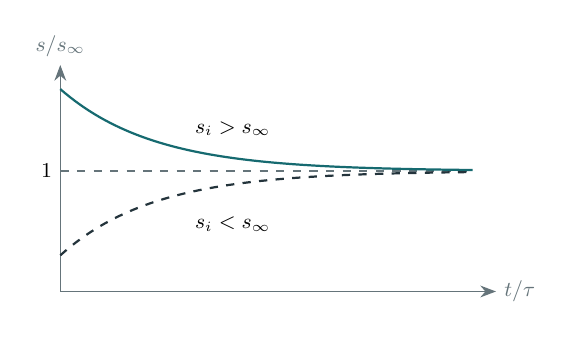
\begin{tikzpicture}[scale=.85,transform shape]
\begin{scope}[x=1.4cm,y=1.8cm]
\draw[axis](0,0)--(4.65,0)node[right]{$t/\tau$};
\draw[axis](0,0)--(0,1.88)node[above]{$s/s_\infty$};
\draw[guide](0,1)--(4.4,1);\node[left]at(0,1){$1$};
\draw[traj,domain=0:4.4,samples=84]plot(\x,{1+.68*exp(-\x)});
\draw[object,dashed,domain=0:4.4,samples=84]plot(\x,{1-.70*exp(-\x)});
\node[right]at(1.35,1.35){$s_i>s_\infty$};
\node[right]at(1.35,.56){$s_i<s_\infty$};
\end{scope}
\end{tikzpicture}
\figcaption{变图电4.1V1\quad 初始面电荷在平衡值两侧时，电流方向相反，偏离量都按指数衰减}
\end{minipage}\end{center}
\item 外场在 $t_1$ 撤去时，表面电荷连续。撤场后 $E=-s/\varepsilon_0$，所以以 $s(t_1)$ 为新初值解 $\dot s=-s/\tau$，得 $s=s(t_1)e^{-(t-t_1)/\tau}$、$j=-s/\tau$。若通场和撤场后间隔均为 $T$，先由充电段求 $s(t_1)=s_\infty(1-e^{-T/\tau})$，再乘 $e^{-T/\tau}$。变图电4.1V2以 $t_1=2\tau$ 展示面电荷连续而电流在撤场时反向。
\begin{center}\begin{minipage}{.98\linewidth}\centering
\begin{tikzpicture}[scale=.85,transform shape]
\begin{scope}[x=1.36cm,y=1.45cm]
\draw[axis](0,0)--(4.75,0)node[right]{$t/\tau$};
\draw[axis](0,-1.1)--(0,1.38)node[above]{归一化量};
\draw[traj,domain=0:2,samples=65]plot(\x,{1-exp(-\x)});
\draw[traj,domain=2:4.5,samples=65]plot(\x,{(1-exp(-2))*exp(2-\x)});
\draw[object,dashed,domain=0:2,samples=65]plot(\x,{exp(-\x)});
\draw[object,dashed,domain=2:4.5,samples=65]plot(\x,{-(1-exp(-2))*exp(2-\x)});
\draw[guide](2,-.92)--(2,1.07);
\node[above]at(2,1.07){撤场};\node[left]at(0,1){$1$};
\node[right]at(3.44,.42){$s/s_\infty$};\node[right]at(3.44,-.40){$j/j_0$};
\end{scope}
\end{tikzpicture}
\figcaption{变图电4.1V2\quad 撤场时自由面电荷连续，反场立即使电流反向}
\end{minipage}\end{center}
\item 介电常量改为 $\varepsilon$，并取线性、均匀、即时的介电响应。端面储存的是自由电荷，反场改为 $s/\varepsilon$，故 $\dot s=\sigma(E_0-s/\varepsilon)$。由零初值解得 $s=\varepsilon E_0(1-e^{-\sigma t/\varepsilon})$、$j=\sigma E_0e^{-\sigma t/\varepsilon}$。变图电4.1V3以 $\varepsilon_1=2\varepsilon_0$ 对照，最终自由面密度与时间常数成同一倍数变化，初始电流密度保持 $\sigma E_0$。
\begin{center}\begin{minipage}{.98\linewidth}\centering
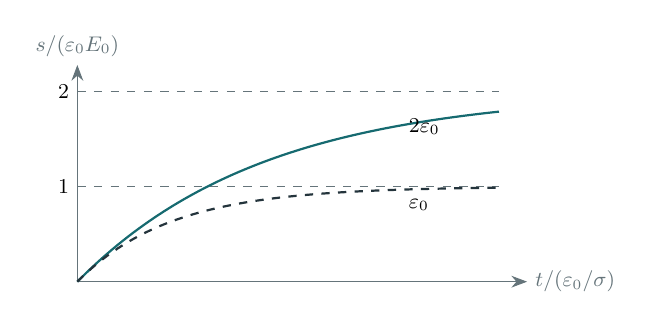
\begin{tikzpicture}[scale=.85,transform shape]
\begin{scope}[x=1.4cm,y=1.42cm]
\draw[axis](0,0)--(4.8,0)node[right]{$t/(\varepsilon_0/\sigma)$};
\draw[axis](0,0)--(0,2.28)node[above]{$s/(\varepsilon_0 E_0)$};
\draw[guide](0,1)--(4.5,1) (0,2)--(4.5,2);
\node[left]at(0,1){$1$};\node[left]at(0,2){$2$};
\draw[traj,domain=0:4.5,samples=84]plot(\x,{2*(1-exp(-\x/2))});
\draw[object,dashed,domain=0:4.5,samples=84]plot(\x,{1-exp(-\x)});
\node[right]at(3.45,1.63){$2\varepsilon_0$};
\node[right]at(3.45,.81){$\varepsilon_0$};
\end{scope}
\end{tikzpicture}
\figcaption{变图电4.1V3\quad 介电常量改变时，自由面电荷终值和弛豫时间一同改变}
\end{minipage}\end{center}
\item 归一化误差为 $\delta=(s_\infty-s)/s_\infty=j/j_0=e^{-t/\tau}$。取对数后得到变图电4.1V4的直线 $\ln(1/\delta)=t/\tau$。充到终值的 $99\%$ 时 $\delta=0.01$，所以 $t=\tau\ln100\simeq4.605\tau$，电流降为初值的 $1\%$。若容许误差再减为 $0.1\%$，还需 $\tau\ln10$。
\begin{center}\begin{minipage}{.98\linewidth}\centering
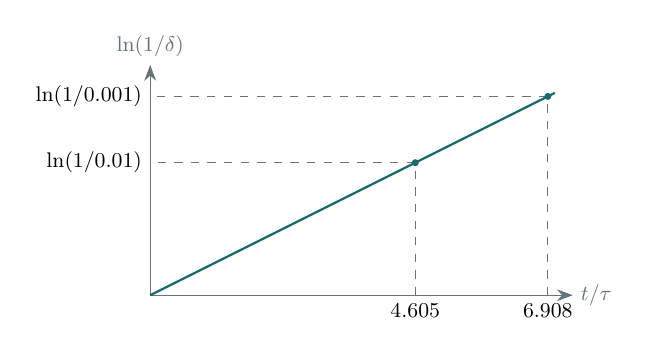
\begin{tikzpicture}[scale=.85,transform shape]
\begin{scope}[x=.86cm,y=.43cm]
\draw[axis](0,0)--(7.34,0)node[right]{$t/\tau$};
\draw[axis](0,0)--(0,8.0)node[above]{$\ln(1/\delta)$};
\draw[traj](0,0)--(7.03,7.03);
\foreach \x/\i in {4.60517/0.01,6.90776/0.001}{
\draw[guide](\x,0)--(\x,\x)--(0,\x);
\fill[accent](\x,\x)circle(1.5pt);
\node[left]at(0,\x){$\ln(1/\i)$};}
\node[below]at(4.60517,0){$4.605$};\node[below]at(6.90776,0){$6.908$};
\end{scope}
\end{tikzpicture}
\figcaption{变图电4.1V4\quad 误差每缩小一个十倍，所需时间恒为一次时间常数乘自然对数10}
\end{minipage}\end{center}
\item 任意给定外场 $E_a(t)$ 时，方程为 $\tau\dot s+s=\varepsilon_0E_a(t)$。乘积分因子并由 $s(0)=s_i$ 得
\[
s(t)=s_i e^{-t/\tau}+\frac{\varepsilon_0}{\tau}\int_0^t e^{-(t-u)/\tau}E_a(u)\,\dd u.
\]
变图电4.1V5取 $E_a=kt$ 且 $s_i=0$，积分为 $s=\varepsilon_0k(t-\tau+\tau e^{-t/\tau})$。直线表示同一时刻的静态面密度，弛豫曲线在它下方；外场停止后，积分只保留此前驱动的贡献。
\begin{center}\begin{minipage}{.98\linewidth}\centering
\begin{tikzpicture}[scale=.85,transform shape]
\begin{scope}[x=1.4cm,y=0.68cm]
\draw[axis](0,0)--(4.72,0)node[right]{$t/\tau$};
\draw[axis](0,0)--(0,4.94)node[above]{$s/(\varepsilon_0 k\tau)$};
\draw[traj,domain=0:4.4,samples=84]plot(\x,{\x-1+exp(-\x)});
\draw[object,dashed,domain=0:4.4,samples=84]plot(\x,{\x});
\node[above left]at(3.25,3.25){瞬时平衡};
\node[right]at(3.27,2.17){实际面密度};
\end{scope}
\end{tikzpicture}
\figcaption{变图电4.1V5\quad 斜坡外场下，表面电荷逐渐形成，有限弛豫时间表现为滞后}
\end{minipage}\end{center}
\item 若 $E_a=E_m\cos\omega t$，设稳态 $s=A\cos\omega t+B\sin\omega t$。比较余弦和正弦系数得 $A+\omega\tau B=\varepsilon_0E_m$、$B-\omega\tau A=0$，所以
\[
s=\frac{\varepsilon_0E_m}{\sqrt{1+\omega^2\tau^2}}\cos(\omega t-\phi),\quad
\tan\phi=\omega\tau,\quad
j=-\frac{\omega\varepsilon_0E_m}{\sqrt{1+\omega^2\tau^2}}\sin(\omega t-\phi).
\]
变图电4.1V6取 $\omega\tau=1$，电荷幅值为低频静态幅值的 $1/\sqrt2$，峰位滞后 $\pi/4$。该周期解适用于准静态且电导率可视为常量的频率范围。
\begin{center}\begin{minipage}{.98\linewidth}\centering
\begin{tikzpicture}[scale=.85,transform shape]
\begin{scope}[x=1.0cm,y=1.25cm]
\draw[axis](0,0)--(6.6,0)node[right]{$\omega t$};
\draw[axis](0,-1.18)--(0,1.2)node[above]{归一化量};
\draw[object,dashed,domain=0:6.28,samples=84]plot(\x,{cos(deg(\x))});
\draw[traj,domain=0:6.28,samples=84]plot(\x,{cos(deg(\x)-45)/sqrt(2)});
\draw[guide](.785398,0)--(.785398,.707107);
\node[below right]at(.785398,0){$\pi/4$};
\node[right]at(4.62,-.68){$s/(\varepsilon_0E_m)$};
\node[above left]at(6.24,1){$E_a/E_m$};
\end{scope}
\end{tikzpicture}
\figcaption{变图电4.1V6\quad 周期稳态中自由面电荷的幅值减小，峰值相对外场延后}
\end{minipage}\end{center}
\item 取平面导体厚 $d$、面积 $A$，变图电4.1V7把 $U_a=E_0d$ 分到导电压降与面电荷反场。取 $R_c=d/(\sigma A)$、$C=\varepsilon_0A/d$、$Q=sA$。沿回路写 $R_c\dot Q+Q/C=U_a$，时间常数为 $R_cC=\varepsilon_0/\sigma$。当面积增加时，电阻按面积反比减小，电容按面积正比增大；二者相抵。
\begin{center}\begin{minipage}{.98\linewidth}\centering
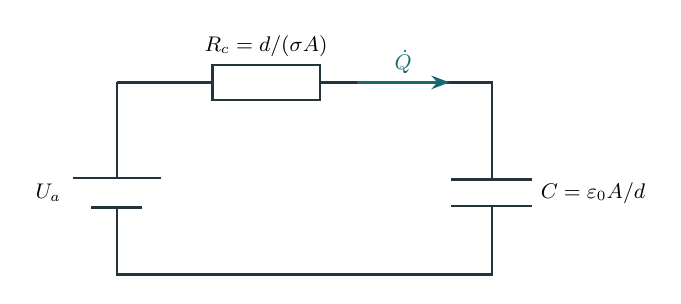
\begin{tikzpicture}[scale=.85,transform shape]
\draw[object](0,1.65)--(1.43,1.65) (3.03,1.65)--(5.6,1.65)--(5.6,.20) (5.6,-.20)--(5.6,-1.22)--(0,-1.22)--(0,-.22) (0,.22)--(0,1.65);
\draw[object](1.43,1.39)rectangle(3.03,1.91);
\node[above]at(2.23,1.91){$R_c=d/(\sigma A)$};
\draw[object](4.99,.20)--(6.21,.20) (4.99,-.20)--(6.21,-.20);
\node[right]at(6.21,0){$C=\varepsilon_0A/d$};
\draw[object](-.66,.22)--(.66,.22) (-.38,-.22)--(.38,-.22);
\node[left]at(-.71,0){$U_a$};
\draw[motion](3.59,1.65)--(4.97,1.65)node[midway,above]{$\dot Q$};
\end{tikzpicture}
\figcaption{变图电4.1V7\quad 外场驱动电压分别平衡传导电阻压降和积累电荷的反向电压}
\end{minipage}\end{center}
\item 瞬时焦耳功率为 $P_J=P_J(0)e^{-2t/\tau}$，其中 $P_J(0)=\sigma E_0^2Ad$。变图电4.1V8在 $T$ 左右分割功率曲线下的面积，分别积分得
\[
Q_J(0,T)=\frac12\varepsilon_0 E_0^2Ad(1-e^{-2T/\tau}),\qquad
Q_J(T,\infty)=\frac12\varepsilon_0 E_0^2Ad\,e^{-2T/\tau}.
\]
剩余焦耳热的相对量为 $e^{-2T/\tau}$，面电荷偏离终值的相对量为 $e^{-T/\tau}$。达到相同相对阈值时，热量所需的等待时间是面密度的一半。
\begin{center}\begin{minipage}{.98\linewidth}\centering
\begin{tikzpicture}[scale=.85,transform shape]
\begin{scope}[x=1.77cm,y=2.5cm]
\fill[accent!31](0,0)--plot[domain=0:.8,samples=40](\x,{exp(-2*\x)})--(.8,0)--cycle;
\fill[warm!40](.8,0)--plot[domain=.8:3.5,samples=65](\x,{exp(-2*\x)})--(3.5,0)--cycle;
\draw[axis](0,0)--(3.76,0)node[right]{$t/\tau$};
\draw[axis](0,0)--(0,1.15)node[above]{$P_J/P_J(0)$};
\draw[traj,domain=0:3.5,samples=85]plot(\x,{exp(-2*\x)});
\draw[guide](.8,0)--(.8,.201897);
\node[below]at(.8,0){$T/\tau$};
\node[above right]at(.13,.76){已产生的热};
\node[above right]at(1.25,.18){余下的热};
\end{scope}
\end{tikzpicture}
\figcaption{变图电4.1V8\quad 功率曲线的两段面积乘功率与时间尺度，分别为已释放和尚未释放的热量}
\end{minipage}\end{center}
\end{enumerate}

\Needspace{13\baselineskip}

\pdfbookmark[2]{第 2 题 分段非均匀电导率中的体电荷和界面电荷}{q2}

\section*{第 2 题\quad 分段非均匀电导率中的体电荷和界面电荷}\label{q:2}

截面积为$S$、长$2L$的圆柱导体沿轴向坐标$x$的电导率为
\[
\sigma(x)=\begin{cases}\sigma_0(1+x/L),&0<x<L,\\\sigma_0(1+2x/L),&L<x<2L.\end{cases}
\]
两端电压$\Delta U=U(0)-U(2L)>0$，稳恒电流沿$+x$均匀通过每个截面。介电响应取真空值$\varepsilon_0$，忽略边缘效应。求总电阻、$x\ne L$处体电荷密度，以及$x=L$处自由面电荷密度。

\begin{center}\begin{minipage}{.98\linewidth}\centering
\begin{tikzpicture}[scale=.9,transform shape]

\fill[accent!8](0,0) rectangle(3,1.8);\fill[warm!10](3,0) rectangle(6,1.8);\draw[object](0,0) rectangle(6,1.8);
\draw[guide](3,-.2)--(3,2);\node at(1.5,1.25){$\sigma_0(1+x/L)$};\node at(4.5,1.25){$\sigma_0(1+2x/L)$};
\draw[motion](.7,.55)--(2.2,.55) node[midway,above]{$I$};\node[above] at(0,1.8){$U(0)$};\node[above] at(6,1.8){$U(2L)$};
\draw[axis](-.4,-.55)--(6.5,-.55) node[right]{$x$};\foreach \x/\s in {0/0,3/L,6/{2L}}{\node[below] at(\x,-.55){$\s$};}
\node[right] at(6,1){截面$S$};

\end{tikzpicture}
\figcaption{图电4.2\quad 两段串联，电流通过同一截面积，电导率在中间界面跳变。}
\end{minipage}\end{center}

\Needspace{8\baselineskip}

\pdfbookmark[3]{题型定位}{q2-h0}

\subsection*{题型定位}

一维非均匀导体的稳恒电流、电势及电荷分布。先沿各截面串联求电阻，再用同一电流求分段电场及界面跳变量。

\Needspace{8\baselineskip}

\pdfbookmark[3]{知识点}{q2-h1}

\subsection*{知识点}

沿轴截面不变，稳恒电流密度 $j$ 处处相同。局部 $E=j/\sigma$，电阻积分用 $1/\sigma$。分段体电荷由 $\varepsilon_0 E'$ 给出，界面面电荷由 $\varepsilon_0(E_+-E_-)$ 给出。$U'=-E$，两段电势在界面相接。

\Needspace{8\baselineskip}

\pdfbookmark[3]{物理图像}{q2-h2}

\subsection*{物理图像}

解图电4.2A中电导率递增，场强在各开区间下降，从 $u=1$ 的左极限 $j/(2\sigma_0)$ 跳至右极限 $j/(3\sigma_0)$。解图电4.2B的电势连续且在界面变斜，解图电4.2C的累计电荷则含同一界面上的有限负跳。

\Needspace{8\baselineskip}

\pdfbookmark[3]{解题入口}{q2-h3}

\subsection*{解题入口}

对每段分别积分小电阻 $\dd x/[\sigma(x)S]$，端电压除以总电阻给电流。对 $j/\sigma(x)$ 在段内求导；另在界面画向右、向左的柱面外法线，并取两侧场强极限。最后积分 $U'=-E$ 连起端点和界面。

\Needspace{18\baselineskip}
\pdfbookmark[3]{标准解法}{q2-h4}

\subsection*{标准解法}

图电4.2的电导率在$x=L$由$2\sigma_0$跃变到$3\sigma_0$。各截面通过同一个稳恒电流，截面积也相同，故电流密度 $j$ 为常量。场强随局部电导率变化。定义
\[
k=\ln2+\frac12\ln\frac53=0.94855999\ldots .
\]
把长度$\dd x$的小片看成串联微元，完整积分为
\[
R=\frac1S\int_0^{2L}\frac{\dd x}{\sigma(x)}
=\frac{L}{\sigma_0S}\left(\int_0^1\frac{\dd u}{1+u}+\int_1^2\frac{\dd u}{1+2u}\right)
=\boxed{\frac{kL}{\sigma_0S}}.
\]
因此$I=\sigma_0S\Delta U/(kL)$，$j=\sigma_0\Delta U/(kL)$。解图电4.2A以同一$j$贯穿两段，并画出场强的下降及界面跃变。

\begin{center}\begin{minipage}{.98\linewidth}\centering
\begin{tikzpicture}[scale=.9,transform shape]

\draw[axis](0,0)--(5,0) node[right]{$x/L$};\draw[axis](0,0)--(0,3) node[above]{$E\sigma_0/j$};
\draw[traj,domain=0:1,samples=35] plot({2*\x},{2.5/(1+\x)});
\draw[traj,domain=1:2,samples=35] plot({2*\x},{2.5/(1+2*\x)});
\draw[guide](2,0)--(2,1.5);\fill(2,1.25) circle(1.5pt);\fill(2,.8333) circle(1.5pt);
\node[above right] at(2,1.25){$1/2$};\node[below left] at(2,.8333){$1/3$};\node[below] at(2,0){$1$};\node[below] at(4,0){$2$};
\draw[object](6,0) rectangle(9,2);\draw[guide](7.5,-.2)--(7.5,2.2);\node[above] at(7.5,2.2){$x=L,\ s_L<0$};
\draw[axis](6,1)--(5.5,1);\draw[axis](9,1)--(9.5,1);\node[below] at(6,0){$L^-$};\node[below] at(9,0){$L^+$};
\node[align=center] at(7.5,-.75){高斯面通量\\$[E(L^+)-E(L^-)]S$};

\end{tikzpicture}
\figcaption{解图电4.2A\quad 左图的场强下跳对应负界面电荷；右图明确高斯面两侧的外法线。}
\end{minipage}\end{center}

欧姆定律和一维高斯定律给
\[
E(x)=\frac{j}{\sigma(x)},\qquad \rho_e=\varepsilon_0\frac{\dd E}{\dd x}.
\]
在两段内部逐项求导：
\[
\boxed{\rho_e(x)=\begin{cases}
-\dfrac{\varepsilon_0\Delta U}{kL^2(1+x/L)^2},&0<x<L,\\[3pt]
-\dfrac{2\varepsilon_0\Delta U}{kL^2(1+2x/L)^2},&L<x<2L.
\end{cases}}
\]
电导率递增而$j$不变，场强沿$x$减小，体电荷因而为负。界面两侧场强为
\[
E(L^-)=\frac{j}{2\sigma_0},\qquad E(L^+)=\frac{j}{3\sigma_0}.
\]
取薄柱高斯面，右端外法线沿$+x$、左端沿$-x$，有$[E(L^+)-E(L^-)]S=s_LS/\varepsilon_0$，故
\[
\boxed{s_L=-\frac{\varepsilon_0j}{6\sigma_0}=-\frac{\varepsilon_0\Delta U}{6kL}}.
\]
界面带负电，面密度大小约为 $0.1757\varepsilon_0\Delta U/L$。体密度描述各开区间内场强的连续变化，面密度对应界面处的一次有限跃变。

将两段体电荷与中间界面电荷按单位截面积相加，得到：
\[
\int_{0^+}^{L^-}\rho_e\dd x+s_L+\int_{L^+}^{2L^-}\rho_e\dd x
=\varepsilon_0[E(2L^-)-E(0^+)]
=-\frac{4\varepsilon_0j}{5\sigma_0}.
\]
这里的积分区间从左端内侧延伸到右端内侧。导体两端与外接装置交界处的面电荷由各端面两侧的电场决定。

\begin{center}\begin{minipage}{.97\linewidth}\centering
\begin{tikzpicture}[x=2.65cm,y=2.7cm,font=\small]
\draw[axis](0,0)--(2.3,0)node[below right]{$u=x/L$};
\draw[axis](0,0)--(0,1.25)node[above]{$[U(x)-U(2L)]/\Delta U$};
\draw[traj,domain=0:1,samples=65,variable=\t]plot(\t,{1-ln(1+\t)/.9485599924});
\draw[traj,domain=1:2,samples=65,variable=\t]plot(\t,{1-(ln(2)+.5*ln((1+2*\t)/3))/.9485599924});
\draw[guide](1,0)--(1,.26927)--(0,.26927);
\fill(1,.26927)circle(1.4pt);\node[above right]at(1,.26927){连续，斜率改变};
\node[left]at(0,1){$1$};\node[below]at(1,0){$1$};\node[below]at(2,0){$2$};
\end{tikzpicture}
\figcaption{解图电4.2B　由场强分段积分得到的电势。界面没有有限电势跃变，电势曲线在此连续而不光滑。}
\end{minipage}\end{center}

解图电4.2B画出由$U'=-E$积分得到的电势。在中间界面，两段曲线的电势相接，斜率分别取两侧电场的相反数。令$u=x/L$，在两段分别积分可得
\[
\frac{U(x)-U(2L)}{\Delta U}=\begin{cases}
1-\dfrac{\ln(1+u)}k,&0\le u\le1,\\[3pt]
1-\dfrac{\ln2+\tfrac12\ln[(1+2u)/3]}k,&1\le u\le2.
\end{cases}
\]
两式在$u=1$给同一个$1-\ln2/k$，但左右斜率之比为$3/2$，与A图的场强比相同。
电场虽有有限跃变，跨越趋于零厚度的界面时，其电势积分趋于零。
\begin{center}\begin{minipage}{.97\linewidth}\centering
\begin{tikzpicture}[x=2.65cm,y=3cm,font=\small]
\draw[axis](0,0)--(2.35,0)node[right]{$u=x/L$};
\draw[axis](0,-.95)--(0,.27)node[above]{$q(x)/(\varepsilon_0j/\sigma_0)$};
\draw[traj,domain=0:1,samples=60,variable=\t]plot(\t,{1/(1+\t)-1});
\draw[traj,domain=1:2,samples=60,variable=\t]plot(\t,{1/(1+2*\t)-1});
\draw[force](1,-.5)--(1,-.666667);\draw[guide](0,-.8)--(2,-.8);
\node[left]at(0,-.8){$-4/5$};\node[above left]at(1,-.5){$-1/2$};
\draw[guide](1,-.666667)--(1.25,-.56);\node[right]at(1.25,-.56){$-2/3$};
\node[above]at(1,0){$1$};\node[above]at(2,0){$2$};
\node[right,align=left]at(2.45,-.4){界面增量\\$\Delta q=s_L$};
\end{tikzpicture}
\figcaption{解图电4.2C　从左端内部起累计的单位截面积电荷。曲线在界面向下跳$\varepsilon_0j/(6\sigma_0)$，两端外表面电荷不在此图范围内。}
\end{minipage}\end{center}

解图电4.2C把体电荷积分和界面面电荷放在同一条累计曲线上。
定义$q(x)$为$0^+$到x之间的电荷除以截面积S，若x跨过L就计入$s_L$，由高斯定律有$q(x)=\varepsilon_0[E(x)-E(0^+)]$。
第一段终点$q(L^-)=-\varepsilon_0j/(2\sigma_0)$；跨界面后$q(L^+)=-2\varepsilon_0j/(3\sigma_0)$；第二段再贡献$-2\varepsilon_0j/(15\sigma_0)$，终点为$-4\varepsilon_0j/(5\sigma_0)$。
累计曲线先因两段内各自的负体电荷下降，再将界面的面电荷作为一个单独的下跳计入。

负体电荷和负界面电荷是维持稳恒场分布的静态电荷。任意小段有相同的$jS$流入和流出，因此净积累率为零；局部留下的电荷维持所求的静态场强分布。
界面电荷由场强的跳变量决定。两侧场都沿正x方向，且右侧场强小于左侧，所以从左向右跨界面时场强跳变量为负，面电荷也为负。


\Needspace{8\baselineskip}

\pdfbookmark[3]{关键洞察}{q2-h5}

\subsection*{关键洞察}

稳恒要求每段流入和流出电流相同。已有的体电荷与面电荷由稳恒场的形状决定。固定端压时，均匀地将各处电导率乘 $c$，电场和电荷密度保持原值，电流和耗散功率则乘 $c$。

\Needspace{8\baselineskip}

\pdfbookmark[3]{易错点}{q2-h6}

\subsection*{易错点}

用 $\Delta U/(2L)$ 得到的是平均场。薄柱左右外法线异号，面电荷用右侧场减左侧场。介电常量不同时，$\Delta D_n$ 给自由面电荷，$\varepsilon_0\Delta E_n$ 给总面电荷。

\Needspace{8\baselineskip}

\pdfbookmark[3]{课堂讲解建议}{q2-h7}

\subsection*{课堂讲解建议}

让学生沿解图电4.2A同时标 $j$ 的箭头与 $E$ 的两段幅值。用解图电4.2B定位电压降从哪里积出，再用解图电4.2C把界面处有限的负跳与两段连续下降分别算出。请学生将三个有符号贡献相加并和两端电通量差对应。

改变介电常量时，用变图电4.2V4先按 $D=\varepsilon E$ 判断自由面电荷符号。随后在变图电4.2V8比较自由电荷恰为零时两侧的 $E,D$。

\Needspace{18\baselineskip}
\pdfbookmark[3]{变式训练}{q2-h8}

\subsection*{变式训练}

\begin{enumerate}
\item 若两段同为 $\sigma_0(1+x/L)$，合并串联积分得 $R=L\ln3/(\sigma_0S)$、$j=\sigma_0\Delta U/(L\ln3)$。变图电4.2V1的实线给 $E/(j/\sigma_0)=1/(1+x/L)$，在 $x=L$ 两侧均为 $1/2$，故 $s_L=0$。场强仍沿轴下降，对其求导得 $\rho_e=-\varepsilon_0\Delta U/[L^2\ln3(1+x/L)^2]$。
\begin{center}\begin{minipage}{.98\linewidth}\centering
\begin{tikzpicture}[scale=.85,transform shape]
\begin{scope}[x=2.85cm,y=2.47cm]
\draw[axis](0,0)--(2.28,0)node[right]{$x/L$};
\draw[axis](0,0)--(0,1.18)node[above]{$E/(j/\sigma_0)$};
\draw[guide](1,0)--(1,.65);
\node[below]at(1,0){$1$};\node[below]at(2,0){$2$};
\draw[traj,domain=0:2,samples=85]plot(\x,{1/(1+\x)});
\draw[object,dashed,domain=1:2,samples=55]plot(\x,{1/(1+2*\x)});
\draw[object,dashed](1,.5)--(1,.333333);
\fill[accent](1,.5)circle(1.5pt);
\node[above]at(1.62,.46){连续};
\node[below]at(1.57,.21){阶跃材料};
\end{scope}
\end{tikzpicture}
\figcaption{变图电4.2V1\quad 电导率连续时场强在接合处连续，段内的下降仍对应体电荷}
\end{minipage}\end{center}
\item 将等截面积从 $S$ 增为 $2S$，各段长度和电导率分布保持，端电压不变。变图电4.2V2中下方截面面积加倍，每片 $\dd R$ 减半，总电流成为 $2I$；电流密度仍为 $2I/(2S)=j$。因此两导体的 $E,\rho_e,s_L$ 相同。截面积加倍还使同一段的体电荷与界面电荷总量加倍，耗散由 $I\Delta U$ 增至两倍。
\begin{center}\begin{minipage}{.98\linewidth}\centering
\begin{tikzpicture}[scale=.85,transform shape]
\draw[object](0,1.18)rectangle(5.57,1.99);
\draw[object](0,-.92)rectangle(5.57,.70);
\draw[guide](2.77,1.18)--(2.77,1.99) (2.77,-.92)--(2.77,.70);
\draw[motion](.59,1.57)--(2.28,1.57)node[midway,above]{$I$};
\draw[motion](.59,-.11)--(2.28,-.11)node[midway,above]{$2I$};
\node[right]at(5.58,1.57){$S$};\node[right]at(5.58,-.11){$2S$};
\node[below]at(2.77,-.92){$x=L$};
\node at(4.19,1.57){电压 $\Delta U$};
\node at(4.19,-.11){电压 $\Delta U$};
\end{tikzpicture}
\figcaption{变图电4.2V2\quad 同端电压下，电流与截面积同比例改变，电流密度相同}
\end{minipage}\end{center}
\item 反接电压时保留原来的 $+x$ 方向，取 $j_0=|j|$。变图电4.2V3的反接场强是正接场强关于水平轴的镜像。两个开区间的场强导数和界面右减左的场差一并反号，故 $\rho_e,s_L$ 都由负转正。电阻保持 $R=\Delta U/(jS)$，功率保持 $jS\,\Delta U=\Delta U^2/R$。
\begin{center}\begin{minipage}{.98\linewidth}\centering
\begin{tikzpicture}[scale=.85,transform shape]
\begin{scope}[x=2.87cm,y=1.33cm]
\draw[axis](0,0)--(2.31,0)node[right]{$x/L$};
\draw[axis](0,-1.17)--(0,1.24)node[above]{$E/(j_0/\sigma_0)$};
\foreach \s in {-1,1}{
\draw[traj,domain=0:1,samples=53]plot(\x,{\s/(1+\x)});
\draw[traj,domain=1:2,samples=53]plot(\x,{\s/(1+2*\x)});
\draw[guide](1,{\s/2})--(1,{\s/3});}
\node[above]at(1.56,.31){正接};
\node[below]at(1.56,-.31){反接};
\end{scope}
\end{tikzpicture}
\figcaption{变图电4.2V3\quad 坐标取向固定时，反接电压使场强与两种电荷密度共同反号}
\end{minipage}\end{center}
\item 设两段介电常量各为常数 $\varepsilon_1,\varepsilon_2$。稳恒传导仍给 $E_-/E_+=3/2$，体自由电荷为 $\rho_{fi}=\varepsilon_i E_i'$。以正法线从左到右，界面自由面密度为
\[
s_f=\varepsilon_2E_+-\varepsilon_1E_-=\frac{\varepsilon_1j}{\sigma_0}\left(\frac{\eta}{3}-\frac12\right),\qquad \eta=\frac{\varepsilon_2}{\varepsilon_1}.
\]
变图电4.2V4在 $\eta=3/2$ 处由负转正，故仅凭电导率阶跃方向可判场差，判自由电荷还需介电常量比。
\begin{center}\begin{minipage}{.98\linewidth}\centering
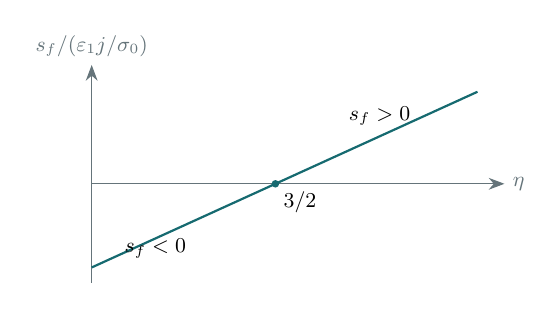
\begin{tikzpicture}[scale=.85,transform shape]
\begin{scope}[x=1.83cm,y=2.5cm]
\draw[axis](0,0)--(3.37,0)node[right]{$\eta$};
\draw[axis](0,-.59)--(0,.71)node[above]{$s_f/(\varepsilon_1j/\sigma_0)$};
\draw[traj](0,-.5)--(3.15,.55);
\fill[accent](1.5,0)circle(1.6pt);
\node[below right]at(1.5,0){$3/2$};
\node[below]at(.52,-.28){$s_f<0$};
\node[above]at(2.35,.30){$s_f>0$};
\end{scope}
\end{tikzpicture}
\figcaption{变图电4.2V4\quad 介电常量比决定电位移跳变的符号}
\end{minipage}\end{center}
\item 设右端电势为零。由 $\Delta U_i=\int E\,\dd x$，两段电压降为 $jL\ln2/\sigma_0$ 和 $jL\ln(5/3)/(2\sigma_0)$，占总电压比例约 $0.731$、$0.269$。变图电4.2V5的两块面积按各自宽度积分后正给这两个比值；从右端回推，$U(L)=\Delta U_2$。从左端算 $U(0)-\Delta U_1$ 也给同一界面值。
\begin{center}\begin{minipage}{.98\linewidth}\centering
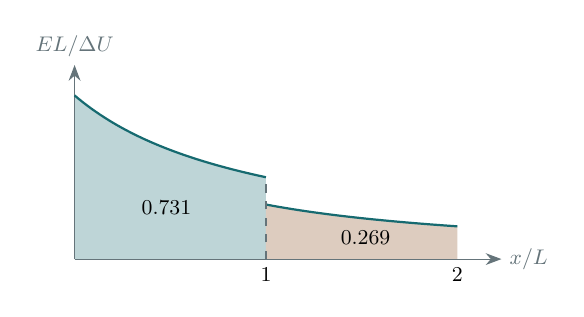
\begin{tikzpicture}[scale=.85,transform shape]
\begin{scope}[x=2.86cm,y=2.32cm]
\fill[accent!28](0,0)--plot[domain=0:1,samples=48](\x,{1/(1+\x)/.94856})--(1,0)--cycle;
\fill[warm!32](1,0)--plot[domain=1:2,samples=48](\x,{1/(1+2*\x)/.94856})--(2,0)--cycle;
\draw[axis](0,0)--(2.23,0)node[right]{$x/L$};
\draw[axis](0,0)--(0,1.25)node[above]{$EL/\Delta U$};
\draw[traj,domain=0:1,samples=55]plot(\x,{1/(1+\x)/.94856});
\draw[traj,domain=1:2,samples=55]plot(\x,{1/(1+2*\x)/.94856});
\draw[guide](1,0)--(1,.5271);
\node at(.48,.33){$0.731$};\node at(1.52,.14){$0.269$};
\node[below]at(1,0){$1$};\node[below]at(2,0){$2$};
\end{scope}
\end{tikzpicture}
\figcaption{变图电4.2V5\quad 归一化电场的面积是各段占总电压的比例}
\end{minipage}\end{center}
\item 从两段端点场差分别算得 $Q_1/S=-\varepsilon_0j/(2\sigma_0)$、$Q_2/S=-2\varepsilon_0j/(15\sigma_0)$。将界面面电荷 $s_L=-\varepsilon_0j/(6\sigma_0)$ 放在两段之间，变图电4.2V6的三次下降合计 $(-1/2-1/6-2/15)\varepsilon_0j/\sigma_0=-4\varepsilon_0j/(5\sigma_0)$，恰等于 $\varepsilon_0[E(2L^-)-E(0^+)]$。
\begin{center}\begin{minipage}{.98\linewidth}\centering
\begin{tikzpicture}[scale=.85,transform shape]
\begin{scope}[x=2.72cm,y=3.55cm]
\draw[axis](0,0)--(2.26,0)node[right]{$x/L$};
\draw[axis](0,-.96)--(0,.19)node[above]{$q/(\varepsilon_0j/\sigma_0)$};
\draw[traj,domain=0:1,samples=48]plot(\x,{1/(1+\x)-1});
\draw[traj,domain=1:2,samples=48]plot(\x,{1/(1+2*\x)-1});
\draw[force](1,-.5)--(1,-.666667);
\node[above]at(.53,-.34){$Q_1/S$};\node[right]at(1,-.56){$s_L$};
\node[below]at(1.6,-.77){$Q_2/S$};
\fill[accent](2,-.8)circle(1.5pt);
\node[right]at(2,-.8){$-4/5$};
\end{scope}
\end{tikzpicture}
\figcaption{变图电4.2V6\quad 累计电荷曲线沿均匀电流方向分段下降，界面电荷给有限下跳}
\end{minipage}\end{center}
\item 微段的耗散为 $\dd P=jES\,\dd x=j^2S\dd x/\sigma(x)$。分段积分后 $P_i=I^2R_i$，故变图电4.2V7的两段功率分别占 $P$ 的约 $73.1\%$ 和 $26.9\%$。保持端电压且把各处 $\sigma$ 乘 $c$ 时，电阻缩为 $R/c$，电流变 $cI$；这两区的电场不变，功率密度 $jE$ 及总功率都乘 $c$。
\begin{center}\begin{minipage}{.98\linewidth}\centering
\begin{tikzpicture}[scale=.85,transform shape]
\draw[axis](0,0)--(7.03,0)node[right]{功率};
\fill[accent!47](0,.61)rectangle(4.465,1.38);
\fill[warm!58](4.465,.61)rectangle(6.11,1.38);
\draw[object](0,.61)rectangle(6.11,1.38);
\node at(2.23,1.0){$P_1=0.731P$};\node at(5.29,1.0){$P_2$};
\draw[guide](4.465,0)--(4.465,.61) (6.11,0)--(6.11,.61);
\node[below]at(4.465,0){$0.731P$};\node[below]at(6.11,0){$P$};
\end{tikzpicture}
\figcaption{变图电4.2V7\quad 两段串联电流相同，较大的电阻段承担较多耗散}
\end{minipage}\end{center}
\item 当 $\varepsilon_2=3\varepsilon_1/2$ 时，变图电4.2V8上两侧电位移都为 $\varepsilon_1j/(2\sigma_0)$，故自由面电荷为零。电场仍从 $j/(2\sigma_0)$ 跳至 $j/(3\sigma_0)$，总面电荷为 $-\varepsilon_0j/(6\sigma_0)$。它正是极化面电荷 $P_--P_+$，因为 $P=D-\varepsilon_0E$，且 $D_+=D_-$。界面两侧电势斜率仍相差 $3/2$。
\begin{center}\begin{minipage}{.98\linewidth}\centering
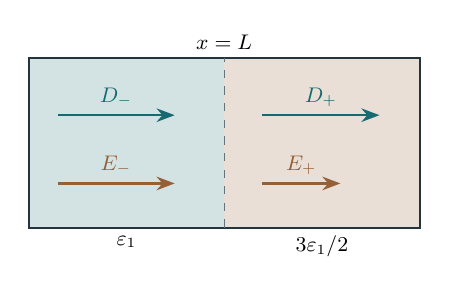
\begin{tikzpicture}[scale=.85,transform shape]
\fill[accent!19](0,0)rectangle(2.92,2.53);
\fill[warm!20](2.92,0)rectangle(5.85,2.53);
\draw[object](0,0)rectangle(5.85,2.53);
\draw[guide](2.92,0)--(2.92,2.53);
\draw[motion](.43,1.68)--(2.18,1.68)node[midway,above]{$D_-$};
\draw[motion](3.49,1.68)--(5.24,1.68)node[midway,above]{$D_+$};
\draw[force](.43,.66)--(2.18,.66)node[midway,above]{$E_-$};
\draw[force](3.49,.66)--(4.656667,.66)node[midway,above]{$E_+$};
\node[below]at(1.46,0){$\varepsilon_1$};\node[below]at(4.38,0){$3\varepsilon_1/2$};
\node[above]at(2.92,2.53){$x=L$};
\end{tikzpicture}
\figcaption{变图电4.2V8\quad 两侧各自的一对电场箭头和一对电位移箭头分别用相同比例绘制}
\end{minipage}\end{center}
\end{enumerate}

\Needspace{13\baselineskip}

\pdfbookmark[2]{第 3 题 球对称大气导电与地面电势}{q3}

\section*{第 3 题\quad 球对称大气导电与地面电势}\label{q:3}

把地球视为半径$R=6.0\times10^6\,\mathrm m$的导体。晴天大气的球对称电导率为$\sigma(r)=\sigma_0+a(r-R)^2$，其中$\sigma_0=3.0\times10^{-14}\,\mathrm{S/m}$，$a=0.5\times10^{-20}\,\mathrm{S/m^3}$。径向向外为正，已知$E(R)=-100\,\mathrm{V/m}$。采用稳态近似，大气电荷分布不变，忽略地球内部体电荷。求流入地面的总电流大小、地面自由面电荷密度、大气体电荷分布，以及大气顶层$r\to\infty$相对地面的电势差。

\begin{center}\begin{minipage}{.98\linewidth}\centering
\begin{tikzpicture}[scale=.9,transform shape]

\fill[accent!8](0,0) circle(1.8);\draw[object](0,0) circle(1.8);\draw[guide](0,0) circle(2.7);
\node at(0,0){地球};\draw[axis](0,0)--(1.273,1.273) node[midway,above left]{$R$};
\foreach \a in {0,90,180,270}{\draw[force](\a:2.5)--(\a:1.95);}
\node[right] at(2.8,1.3){$\rho_e(r)>0$};\node[right] at(2.8,.4){$E_R<0$};\node[right] at(2.8,-.5){$s_R<0$};

\end{tikzpicture}
\figcaption{图电4.3\quad 径向向外为正，地面带负电，大气电场及传导电流向内。}
\end{minipage}\end{center}

\Needspace{8\baselineskip}

\pdfbookmark[3]{题型定位}{q3-h0}

\subsection*{题型定位}

球对称非均匀导电问题。由不同球壳通过的相同电流求电场，用高斯通量差求体电荷，并沿径向积分得到电势差。

\Needspace{8\baselineskip}

\pdfbookmark[3]{知识点}{q3-h1}

\subsection*{知识点}

稳态守恒的是 $4\pi r^2j$。高斯定律给 $\rho_e=\varepsilon_0(r^2E)'/r^2$，而 $Q_{\rm enc}=4\pi\varepsilon_0 r^2E$ 给球面包围电荷。单位厚度的耗散功率为 $4\pi r^2jE$，累计电压则用 $E=-V'$。

\Needspace{8\baselineskip}

\pdfbookmark[3]{物理图像}{q3-h2}

\subsection*{物理图像}

解图电4.3A内外球面面积不同，同一电流摊到不同面积。解图电4.3B中正体密度从地面零值增加，随后下降；解图电4.3C显示其正电荷逐步补偿地面负电荷，有限半径球面包围的净电荷仍为负。

\Needspace{8\baselineskip}

\pdfbookmark[3]{解题入口}{q3-h3}

\subsection*{解题入口}

先取带符号的 $E_R<0$，代地面欧姆关系求总电流。再由 $r^2j$ 恒定得到 $E(r)$，对 $r^2E$ 求导得体密度。对电势积分令 $h=\sqrt{\sigma_0/a}$、$z=r-R$，分式积分时将两个对数合并。

\Needspace{18\baselineskip}
\pdfbookmark[3]{标准解法}{q3-h4}

\subsection*{标准解法}

图电4.3中的电流沿径向向内，同心球面越大，单位面积通过的电流越小。先在地面使用欧姆定律：
\[
j(R)=\sigma_0E_R,\qquad
\boxed{I=4\pi R^2\sigma_0|E_R|\simeq1.36\times10^3\,\mathrm A},
\quad E_R=E(R).
\]
导体内场为零，跨过地面的小高斯柱给
\[
\boxed{s_R=\varepsilon_0E_R=-8.85\times10^{-10}\,\mathrm{C/m^2}}.
\]

\begin{center}\begin{minipage}{.98\linewidth}\centering
\begin{tikzpicture}[scale=.9,transform shape]

\draw[object](0,0) circle(1);\draw[guide](0,0) circle(2);\draw[guide](0,0) circle(2.3);
\draw[axis](0,0)--(2,0) node[midway,below]{$r$};\draw[<->](2,.4)--(2.3,.4);\node[right] at(2.3,.4){$\dd r$};
\draw[force](0,2.7)--(0,1.7) node[left]{$j$};\node at(0,-2.8){$4\pi r^2j(r)=-I$};
\node[align=left] at(6,1){球壳体积$4\pi r^2\dd r$\\外减内的通量\\$4\pi\dd(r^2E)$};
\node[align=left] at(6,-1.2){$\Delta V=-\int_R^\infty E\dd r>0$\\顶层电势高于地面};

\end{tikzpicture}
\figcaption{解图电4.3A\quad 同心球面上的总电流相同；球壳电荷由两面的电通量之差求出。}
\end{minipage}\end{center}

解图电4.3A取半径$r,r+\dd r$的球壳。稳恒电流要求$4\pi r^2j(r)=4\pi R^2j(R)$，所以
\[
j(r)=\sigma_0E_R\frac{R^2}{r^2},\qquad
\boxed{E(r)=\frac{\sigma_0E_RR^2}{r^2[\sigma_0+a(r-R)^2]}}.
\]
用球壳内电荷等于两球面电通量之差，有
\[
\rho_e=\frac{\varepsilon_0}{r^2}\frac{\dd(r^2E)}{\dd r}
=\boxed{-\frac{2\varepsilon_0\sigma_0E_RR^2a(r-R)}{r^2[\sigma_0+a(r-R)^2]^2}}.
\]
由于$E_R<0$，$r>R$的体电荷为正，符合图示。球面的面积随半径增大，展开通量导数得到 $\varepsilon_0(E'+2E/r)$。

电势差按所问的顶层减地面定义：
\[
\Delta V=V(\infty)-V(R)=-\int_R^\infty E(r)\dd r>0.
\]
令$h=\sqrt{\sigma_0/a}$、$z=r-R$，则
\[
\Delta V=-E_RR^2h^2\int_0^\infty\frac{\dd z}{(R+z)^2(z^2+h^2)}.
\]
对被积函数作分式分解，记$D=R^2+h^2$：
\[
\frac1{(R+z)^2(z^2+h^2)}
=\frac{2R}{D^2(R+z)}+\frac1{D(R+z)^2}
-\frac{2Rz}{D^2(z^2+h^2)}+\frac{R^2-h^2}{D^2(z^2+h^2)}.
\]
积分时两个对数的无穷部分相消，结果为
\[
\boxed{\Delta V=-E_R\frac{R^2h^2}{D^2}
\left[\frac D R+2R\ln\frac hR+\frac{\pi(R^2-h^2)}{2h}\right]
\simeq3.83\times10^5\,\mathrm V}.
\]
本题$h\simeq2.45\times10^3\,\mathrm m\ll R$。若在近地主要导电层用$r^2\simeq R^2$，可估为$\Delta V\simeq|E_R|\pi h/2=3.85\times10^5\,\mathrm V$。主要电压降出现在几倍 $h$ 以内，因而用平面面积给出相差约 $0.38\%$ 的近地估算。

再积分体电荷，可得$Q_{\rm atm}=4\pi\varepsilon_0[r^2E]_R^\infty=-4\pi\varepsilon_0R^2E_R$，与地面总负电荷相抵消。这里取地面场强为给定条件，该场强在模型中维持稳态径向电流。

\begin{center}\begin{minipage}{.97\linewidth}\centering
\begin{tikzpicture}[x=1.45cm,y=2.7cm,font=\small]
\draw[axis](0,0)--(4.4,0)node[below right]{$u=(r-R)/h$};
\draw[axis](0,0)--(0,1.25)node[above]{归一化密度与场强};
\draw[traj,domain=0:4,samples=100,variable=\t]plot(\t,{1/((1+\t*\t)*(1+.0004082483*\t)^2)});
\draw[thick,warm,domain=0:4,samples=100,variable=\t]plot(\t,{2*\t/((1+\t*\t)^2*(1+.0004082483*\t)^2)});
\node[left]at(0,1){$1$};\node[below]at(1,0){$1$};\node[below]at(2,0){$2$};
\node[right,accent]at(4.7,.95){$E/E_R$};
\node[right,warm]at(4.7,.5){$\rho_e/(\varepsilon_0|E_R|/h)$};
\end{tikzpicture}
\figcaption{解图电4.3B　按给定球对称模型绘制的场强比与正体电荷密度。两条曲线保留$r^{-2}$因子；场向内，正电荷密度在近地处先升后降。}
\end{minipage}\end{center}

解图电4.3B用$u=(r-R)/h$、$\eta=h/R$将两个空间分布写为
\[
\frac{E}{E_R}=\frac1{(1+u^2)(1+\eta u)^2},\qquad
\frac{\rho_e}{\varepsilon_0|E_R|/h}=\frac{2u}{(1+u^2)^2(1+\eta u)^2}.
\]
图中的 $E/E_R$ 为正，对应向内的负径向场。体密度在地面为零，向上先增大再减小。两条曲线均保留球面面积随高度增长的因子 $(1+\eta u)^{-2}$。
\begin{center}\begin{minipage}{.97\linewidth}\centering
\begin{tikzpicture}[x=1.45cm,y=2.7cm,font=\small]
\draw[axis](0,0)--(4.4,0)node[below right]{$u=(r-R)/h$};
\draw[axis](0,0)--(0,1.25)node[above]{电荷比例};
\draw[traj,domain=0:4,samples=100,variable=\t]plot(\t,{1/(1+\t*\t)});
\draw[thick,warm,domain=0:4,samples=100,variable=\t]plot(\t,{\t*\t/(1+\t*\t)});
\draw[guide](1,0)--(1,.5)--(0,.5);\fill(1,.5)circle(1.4pt);
\node[left]at(0,1){$1$};\node[left]at(0,.5){$1/2$};\node[below]at(1,0){$1$};
\node[right,accent]at(4.7,.85){$Q_{\rm enc}/Q_{\rm g}$};
\node[right,warm]at(4.7,.4){$Q_{\rm atm}(<r)/|Q_{\rm g}|$};
\end{tikzpicture}
\figcaption{解图电4.3C　有限球面内的总负电荷比例与累计大气正电荷比例。两者在高度h处均为1/2，只有到无穷远才完全抵消。}
\end{minipage}\end{center}

解图电4.3C直接回答局部正电荷为何不使电场转向。
记地面总电荷$Q_{\rm g}=4\pi\varepsilon_0R^2E_R<0$，由半径r球面的高斯定律可得
\[
Q_{\rm enc}(r)=4\pi\varepsilon_0r^2E(r)=\frac{Q_{\rm g}}{1+u^2},\qquad
Q_{\rm atm}(<r)=Q_{\rm enc}-Q_{\rm g}=|Q_{\rm g}|\frac{u^2}{1+u^2}.
\]
任意有限u下$Q_{\rm enc}<0$，所以场仍指向地心；累计正电荷只是逐渐削弱包围的净负电荷。
在$u=1$处，半数大气正电荷已位于高度h以下，而其余一半分布在更高处。两个电荷比例互补是精确关系，球面积因子在高斯通量中已经约去，无需再作近地近似。

用被积函数比较完整电势和近地估算。令$z=hu$，被积函数中$R^2/(R+z)^2\le1$，故
$0<\Delta V<|E_R|\pi h/2$；平面近似必偏大。
用题给参数，球对称表达式给 $I\simeq1357.2\,\mathrm A$、$\Delta V\simeq3.833\times10^5\,\mathrm V$。由于电势沿外径向增加，电场和电流都指向地面。


\Needspace{8\baselineskip}

\pdfbookmark[3]{关键洞察}{q3-h5}

\subsection*{关键洞察}

局部电荷密度由径向通量变化确定，电场方向由包围净电荷确定。累计电荷的球面积在高斯通量中消去，累计功率使用 $I|E|$ 作积分权重。近地平面估算略去面积随高度增长，给电势差上界。

\Needspace{8\baselineskip}

\pdfbookmark[3]{易错点}{q3-h6}

\subsection*{易错点}

径向正向取向外，流入地面的总电流大小为正，而 $j<0$。球对称散度包含 $2E/r$。部分分式中的两个对数在同一积分上限合并。定义的是顶层减地面电势，因而要对 $-E$ 积分。

\Needspace{8\baselineskip}

\pdfbookmark[3]{课堂讲解建议}{q3-h7}

\subsection*{课堂讲解建议}

在解图电4.3A圈出两个球面，让学生标各自的面积和通过电流。在解图电4.3B辨认电场幅值与正电荷密度的峰位，再用解图电4.3C说明正体电荷与向内场可以同时存在。对应任一高度，请学生写出包围净电荷怎样由地面负电荷和大气正电荷组成。

最后用变图电4.3V8在同一高度读正电荷与焦耳功率的累计比例。用变图电4.3V7解释忽略球面积后，对电压积分每一层的权重怎样改变。

\Needspace{18\baselineskip}
\pdfbookmark[3]{变式训练}{q3-h8}

\subsection*{变式训练}

\begin{enumerate}
\item 若电导率恒为 $\sigma_0$，有 $E=E_R(R/r)^2$，因而 $r^2E$ 恒定。变图电4.3V1把球面半径增大后的电通量画为同一水平线，任意厚球壳的体电荷为零。沿径向积分
\[
V(\infty)-V(R)=-E_R R^2\int_R^\infty r^{-2}\,\dd r=-E_R R=6.0\times10^8\,\mathrm V.
\]
无穷远球面包围的净电荷仍为地面总负电荷，电势采用半径 $R$ 的尺度。
\begin{center}\begin{minipage}{.98\linewidth}\centering
\begin{tikzpicture}[scale=.85,transform shape]
\draw[axis](0,0)--(6.2,0)node[right]{$r/R$};
\draw[axis](0,0)--(0,2.89)node[above]{归一化电通量};
\draw[traj](1.11,2.17)--(5.77,2.17);
\draw[guide](1.11,0)--(1.11,2.17);
\fill[accent](1.11,2.17)circle(1.6pt);
\node[right]at(2.75,2.19){$r^2E/(R^2E_R)=1$};
\node[below]at(1.11,0){$1$};
\node[left]at(0,2.17){$1$};
\end{tikzpicture}
\figcaption{变图电4.3V1\quad 电导率均匀时，每一球壳内外的电通量相等}
\end{minipage}\end{center}
\item 若大气层截于 $R+H$，按 $-\int_R^{R+H}E\,\dd r$ 计算。在 $H\ll R$ 内把球面积近似为地面面积，令 $u=z/h$，则
\[
\Delta V(H)\simeq |E_R|h\int_0^{H/h}\frac{\dd u}{1+u^2}
=|E_R|h\arctan(H/h).
\]
变图电4.3V2中 $H=h$ 时达到平面无穷层电压的一半。取 $h\ll H\ll R$ 可让反正切接近 $\pi/2$，同时令有限区间内的球面积变化较小。
\begin{center}\begin{minipage}{.98\linewidth}\centering
\begin{tikzpicture}[scale=.85,transform shape]
\begin{scope}[x=1.37cm,y=2.5cm]
\draw[axis](0,0)--(4.4,0)node[right]{$H/h$};
\draw[axis](0,0)--(0,1.22)node[above]{$\Delta V(H)/\Delta V_{\text{平面}}(\infty)$};
\draw[guide](0,1)--(4.2,1);
\draw[traj,domain=0:4.2,samples=96]plot(\x,{2*atan(\x)/180});
\draw[guide](1,0)--(1,.5)--(0,.5);
\fill[accent](1,.5)circle(1.55pt);
\node[below]at(1,0){$1$};\node[left]at(0,.5){$1/2$};\node[left]at(0,1){$1$};
\end{scope}
\end{tikzpicture}
\figcaption{变图电4.3V2\quad 近地平面近似下，有限大气层的电压随高度按反正切增加}
\end{minipage}\end{center}
\item 固定电导率分布，只把地面场的幅值乘 $k>0$。由 $r^2j$ 的地面值，$I,j,E$ 都乘 $k$，高斯定律及电势积分给 $s_R,\rho_e,\Delta V$ 同倍变化。变图电4.3V3以 $k=2$ 为例，电压与电流各加倍，功率 $P=I\Delta V$ 则增至四倍。任一壳层的焦耳功率密度同样按 $jE$ 乘 $k^2$。
\begin{center}\begin{minipage}{.98\linewidth}\centering
\begin{tikzpicture}[scale=.85,transform shape]
\draw[axis](0,0)--(5.92,0)node[right]{缩放量};
\draw[axis](0,0)--(0,3.16)node[above]{相对初值};
\draw[guide](0,.65)--(5.62,.65);
\foreach \x/\h/\l in {1.4/1.3/{\Delta V},3.05/1.3/{I},4.72/2.6/{P}}{
\fill[accent!35]({\x-.33},0)rectangle({\x+.33},\h);
\node[below]at(\x,0){$\l$};}
\node[left]at(0,.65){$1$};\node[left]at(0,1.3){$2$};\node[left]at(0,2.6){$4$};
\node[above]at(4.70,2.62){$I\Delta V$};
\end{tikzpicture}
\figcaption{变图电4.3V3\quad 地面场强加倍后，电压和电流线性增加，焦耳功率按平方增加}
\end{minipage}\end{center}
\item 径向向外为正，$j(r)=-I/(4\pi r^2)$。变图电4.3V4中一层厚 $\dd r$ 的空气体积为 $4\pi r^2\dd r$，故
\[
\dd P=jE\,4\pi r^2\dd r=-IE\,\dd r>0,\qquad
P=-I\int_R^\infty E\,\dd r=I\Delta V.
\]
以 $I\simeq1357.2\,\mathrm A$、$\Delta V\simeq3.833\times10^5\,\mathrm V$ 代入，得约 $5.20\times10^8\,\mathrm W$。
\begin{center}\begin{minipage}{.98\linewidth}\centering
\begin{tikzpicture}[scale=.85,transform shape]
\coordinate (O) at(0,0);
\draw[object](O)circle(1.06);
\draw[guide](O)circle(1.51);
\draw[traj](O)circle(1.78);
\draw[object,<->](223:1.51)--(223:1.78)node[left]{$\dd r$};
\draw[force](2.41,.34)--(1.34,.34)node[above,midway]{$j,E$};
\draw[guide](1.57,-.87)--(3.47,-.87)node[right]{$\dd P=-IE\,\dd r$};
\node at(0,0){地球};
\end{tikzpicture}
\figcaption{变图电4.3V4\quad 径向壳层的面积因子与电流密度的半径因子相消}
\end{minipage}\end{center}
\item 要累计高度 $H$ 以下的正电荷，先算半径 $R+H$ 处的包围电荷，再减去地面电荷。变图电4.3V5的曲线是 $Q_{\rm atm}(<H)/|Q_{\rm g}|=u_H^2/(1+u_H^2)$，$u_H=H/h$。令比值为 $0.9$，有 $u_H^2=9$，所以 $H=3h\simeq7.35\,\mathrm{km}$。高斯通量中已消去半径面积因子，这里的 $3h$ 来自完整球对称模型。
\begin{center}\begin{minipage}{.98\linewidth}\centering
\begin{tikzpicture}[scale=.85,transform shape]
\begin{scope}[x=1.35cm,y=2.65cm]
\draw[axis](0,0)--(4.45,0)node[right]{$H/h$};
\draw[axis](0,0)--(0,1.17)node[above]{$Q_{\rm atm}(<H)/|Q_{\rm g}|$};
\draw[traj,domain=0:4.2,samples=96]plot(\x,{(\x)^2/(1+(\x)^2)});
\draw[guide](3,0)--(3,.9)--(0,.9);
\fill[accent](3,.9)circle(1.6pt);
\node[below]at(3,0){$3$};\node[left]at(0,.9){$0.9$};
\end{scope}
\end{tikzpicture}
\figcaption{变图电4.3V5\quad 包含九成大气正电荷的高度由累计电荷曲线读出}
\end{minipage}\end{center}
\item 求体电荷峰值。对 $2u/[(1+u^2)^2(1+\eta u)^2]$ 取对数求导，极值满足 $1/u-4u/(1+u^2)-2\eta/(1+\eta u)=0$，即
\[
1-3u^2-\eta u-5\eta u^3=0.
\]
左端由1严格下降至负值，故正根唯一。近地取 $\eta=0$ 得 $u=1/\sqrt3$，约在 $1.41\,\mathrm{km}$，球几何使根略向左。变图电4.3V6用实际 $\eta$ 画密度，并标出峰位和累计一半电荷的 $u=1$。
\begin{center}\begin{minipage}{.98\linewidth}\centering
\begin{tikzpicture}[scale=.85,transform shape]
\begin{scope}[x=2.44cm,y=3.45cm]
\draw[axis](0,0)--(2.59,0)node[right]{$u$};
\draw[axis](0,0)--(0,.82)node[above]{$\rho_e/(\varepsilon_0|E_R|/h)$};
\draw[traj,domain=0:2.42,samples=96]plot(\x,{2*\x/((1+(\x)^2)^2*(1+.000408248*\x)^2)});
\draw[guide](0.577169,0)--(0.577169,0.649213) (1,0)--(1,.4996);
\fill[accent](0.577169,0.649213)circle(1.6pt);
\node[above]at(0.577169,0.649213){峰位};
\node[below]at(0.577169,0){$0.577$};\node[below]at(1,0){$1$};
\end{scope}
\end{tikzpicture}
\figcaption{变图电4.3V6\quad 体密度最大处和累计电荷到一半的位置不同}
\end{minipage}\end{center}
\item 令 $\eta=h/R$。变图电4.3V7中平面和球对称被积函数的差来自乘子 $(1+\eta u)^{-2}$，后者小于1，故平面估算偏高。用精确积分式先将对数合并，再求小 $\eta$ 极限，可写
\[
\frac{\Delta V}{|E_R|h}
=\frac{\tfrac{\pi}{2}(1-\eta^2)+\eta(1+\eta^2+2\ln\eta)}{(1+\eta^2)^2}.
\]
相对于平面结果的差在首阶为 $2\eta[2\ln(1/\eta)-1]/\pi$。对题设参数，平面估计约高 $0.38\%$。图中取较大的 $\eta$ 显示两曲线间距，以便观察高处的球面权重。
\begin{center}\begin{minipage}{.98\linewidth}\centering
\begin{tikzpicture}[scale=.85,transform shape]
\begin{scope}[x=1.36cm,y=2.53cm]
\draw[axis](0,0)--(4.43,0)node[right]{$u$};
\draw[axis](0,0)--(0,1.14)node[above]{归一化被积函数};
\draw[object,dashed,domain=0:4.2,samples=96]plot(\x,{1/(1+(\x)^2)});
\draw[traj,domain=0:4.2,samples=96]plot(\x,{1/((1+(\x)^2)*(1+.14*\x)^2)});
\node[above right]at(1.08,.47){平面};
\node[below]at(1.24,.25){球对称，示意 $\eta=0.14$};
\end{scope}
\end{tikzpicture}
\figcaption{变图电4.3V7\quad 球面积随高度增大，同一高度处的电势积分权重较小}
\end{minipage}\end{center}
\item 由 $P(H)=\int_R^{R+H}(-IE)\,\dd r$ 得 $P(H)=I[V(R+H)-V(R)]$，因此累计功率比例精确等于累计电压比例。用平面估计，变图电4.3V8给 $P(H)/P(\infty)\simeq2\arctan(H/h)/\pi$。在 $H=h$ 处约为 $1/2$，在 $H=3h$ 处约为 $0.795$；同一 $3h$ 高度已累计 $0.90$ 的大气正电荷。
\begin{center}\begin{minipage}{.98\linewidth}\centering
\begin{tikzpicture}[scale=.85,transform shape]
\begin{scope}[x=1.36cm,y=2.68cm]
\draw[axis](0,0)--(4.4,0)node[right]{$H/h$};
\draw[axis](0,0)--(0,1.24)node[above]{累计比例};
\draw[traj,domain=0:4.18,samples=96]plot(\x,{(\x)^2/(1+(\x)^2)});
\draw[object,dashed,domain=0:4.18,samples=96]plot(\x,{2*atan(\x)/180});
\draw[guide](3,0)--(3,.9);
\fill[accent](3,.9)circle(1.55pt) (3,.795167)circle(1.55pt);
\node[above left]at(3,.907){正电荷 $0.90$};
\node[below left]at(3,.771){功率约 $0.795$};
\node[below]at(3,0){$3$};
\end{scope}
\end{tikzpicture}
\figcaption{变图电4.3V8\quad 相同高度下，累计电荷和累计焦耳功率由不同的物理权重决定}
\end{minipage}\end{center}
\end{enumerate}

\Needspace{13\baselineskip}

\pdfbookmark[2]{第 4 题 双层漏电介质球的界面电荷}{q4}

\section*{第 4 题\quad 双层漏电介质球的界面电荷}\label{q:4}

半径$R_1$以内为均匀介质$(\varepsilon_1,\sigma_1)$，$R_1<r<R_2$为介质$(\varepsilon_2,\sigma_2)$，外部为真空；$\sigma_1,\sigma_2>0$。初始自由体电荷密度为$\rho_0$（$r<R_1$）及0（球壳内），两界面初始自由面电荷均为零。外部无导电通路。求$R_1,R_2$两球面的自由面电荷密度随时间的变化。

\begin{center}\begin{minipage}{.98\linewidth}\centering
\begin{tikzpicture}[scale=.9,transform shape]

\fill[warm!9](0,0) circle(2.4);\fill[accent!12](0,0) circle(1.3);\draw[object](0,0) circle(1.3);\draw[object](0,0) circle(2.4);
\draw[axis](0,0)--(0,1.3) node[midway,left]{$R_1$};\draw[axis](0,0)--(2.4,0) node[midway,below]{$R_2$};
\node[align=left] at(5,1.5){内球：$\varepsilon_1,\sigma_1,\rho_0$\\球壳：$\varepsilon_2,\sigma_2,\rho_e(0)=0$};
\node[align=left] at(5,-.6){两界面初始$s_1=s_2=0$\\外部真空，无导电电流};

\end{tikzpicture}
\figcaption{图电4.4\quad 体电荷与两个球面的自由面电荷分别追踪。}
\end{minipage}\end{center}

\Needspace{8\baselineskip}

\pdfbookmark[3]{题型定位}{q4-h0}

\subsection*{题型定位}

两种漏电介质的球对称电荷弛豫。先求内球体电荷，再用内界面两侧的传导电流与总电荷守恒求两个面电荷。

\Needspace{8\baselineskip}

\pdfbookmark[3]{知识点}{q4-h1}

\subsection*{知识点}

均匀介质内 $\dot\rho_e=-\rho_e/\tau_i$，$\tau_i=\varepsilon_i/\sigma_i$，并有 $j=D/\tau_i$。界面处 $D_+-D_-=s$，$\dot s=j_--j_+$。整个球外无导电通路，体电荷和两界面电荷的代数和固定。

\Needspace{8\baselineskip}

\pdfbookmark[3]{物理图像}{q4-h2}

\subsection*{物理图像}

解图电4.4A所示薄球壳一端从内球收电荷，另一端向外球壳送电荷，差额积在 $R_1$。解图电4.4B按总电荷尺度表示三项。解图电4.4C画同一时刻的三段 $D$，以界面右限减左限求相应面密度。

\Needspace{8\baselineskip}

\pdfbookmark[3]{解题入口}{q4-h3}

\subsection*{解题入口}

由连续性和高斯定律先求每一均匀层的体电荷。用高斯面写 $D_{1-}$ 与 $D_{1+}=D_{1-}+s_1$，把两侧 $j=D/\tau_i$ 代入守恒并乘积分因子。再把内球与内界面的总电荷从 $Q_0$ 扣除，所得电荷分到外球面积。

\Needspace{18\baselineskip}
\pdfbookmark[3]{标准解法}{q4-h4}

\subsection*{标准解法}

用$s_1,s_2$表示图电4.4中两界面向外法线定义的自由面密度，$\tau_i=\varepsilon_i/\sigma_i$。在各均匀介质内部，连续性、高斯定律及欧姆关系给
\[
\frac{\partial\rho_e}{\partial t}=-\nabla\cdot\vect j
=-\frac{\sigma_i}{\varepsilon_i}\rho_e,
\qquad
\rho_e(r,t)=\begin{cases}\rho_0e^{-t/\tau_1},&r<R_1,\\0,&R_1<r<R_2.\end{cases}
\]
在球壳内部，体电荷恒为零，所以径向电流的散度也为零。同一时刻各个同心球面的总电流相同，电流密度随半径按$1/r^2$变化。内界面两侧的电流密度之差则决定面电荷的变化率。

\begin{center}\begin{minipage}{.98\linewidth}\centering
\begin{tikzpicture}[scale=.9,transform shape]

\fill[accent!8](0,0) rectangle(2,2);\fill[warm!8](2,0) rectangle(4,2);\draw[object](2,-.3)--(2,2.5);
\node[above] at(2,2.5){$R_1$界面};\node at(.7,1.6){内侧};\node at(3.2,1.6){外侧};
\draw[motion](.3,.8)--(1.7,.8) node[midway,below]{$j_{1-}$};\draw[motion](2.3,.8)--(3.7,.8) node[midway,below]{$j_{1+}$};
\node at(2,-.9){$\dot s_1=j_{1-}-j_{1+}$};
\node[align=left] at(7,1.3){$D_{1+}=D_{1-}+s_1$\\$j_{1+}=D_{1+}/\tau_2$\\$Q_{\text{体}}+Q_{s_1}+Q_{s_2}=Q_0$};

\end{tikzpicture}
\figcaption{解图电4.4A\quad 两侧电流密度之差给出内界面面电荷的变化率，外侧电位移由内层体电荷和界面电荷共同确定。}
\end{minipage}\end{center}

解图电4.4A取紧贴$R_1$两侧的薄球壳。内侧电位移为$D_{1-}=R_1\rho_0e^{-t/\tau_1}/3$；外侧包含界面电荷，所以$D_{1+}=D_{1-}+s_1$。因此
\[
j_{1-}=\frac{R_1\rho_0}{3\tau_1}e^{-t/\tau_1},\qquad
j_{1+}=\frac{R_1\rho_0}{3\tau_2}e^{-t/\tau_1}+\frac{s_1}{\tau_2}.
\]
对界面作流入减流出的守恒：
\[
\dot s_1+\frac{s_1}{\tau_2}
=\frac{R_1\rho_0}{3}\left(\frac1{\tau_1}-\frac1{\tau_2}\right)e^{-t/\tau_1},\quad s_1(0)=0.
\]
当$\tau_1\ne\tau_2$时，乘$e^{t/\tau_2}$后积分，指数积分系数与右端的时间常数差相消：
\[
\boxed{s_1(t)=\frac{R_1\rho_0}{3}(e^{-t/\tau_2}-e^{-t/\tau_1})}.
\]
若$\tau_1=\tau_2$，右端严格为零，直接由初值知$s_1=0$，与上式连续相符，无需引入发散的辅助时间常数。

再求外界面电荷。整个系统的总自由电荷$Q_0=4\pi R_1^3\rho_0/3$保持不变。$R_2^-$包围的体电荷及内界面电荷合计为
\[
Q_{<R_2}=\frac{4\pi R_1^3\rho_0}{3}e^{-t/\tau_1}+4\pi R_1^2s_1
=Q_0e^{-t/\tau_2}.
\]
剩余电荷只能积在$R_2$上，故
\[
\boxed{s_2(t)=\frac{R_1^3\rho_0}{3R_2^2}(1-e^{-t/\tau_2})}.
\]
由$j_{2-}=D(R_2^-)/\tau_2$积分也给同一结果，外侧真空电流为零。对$\rho_0>0$，$s_1$的符号取决于两种弛豫时间的大小，$s_2$始终非负；足够晚时$s_1\to0$，全部自由电荷迁至外表面。

球壳内的电位移为$D(r,t)=Q_0e^{-t/\tau_2}/(4\pi r^2)$，球外为$Q_0/(4\pi r^2)$。界面自由面电荷由两侧$D$的法向分量之差给出；两侧各用本侧的介电常量将$D$换成$E$。


为把场、电流和界面电荷的计算连起来，可将四个基本关系并列写为
\[
\nabla\cdot\boldsymbol D=\rho_e,\quad \boldsymbol D=\varepsilon_i\boldsymbol E,\quad
\boldsymbol j=\sigma_i\boldsymbol E,\quad \partial_t\rho_e+\nabla\cdot\boldsymbol j=0.
\]
每层内的$\varepsilon_i,\sigma_i$均为常数，故$\nabla\cdot\boldsymbol j=(\sigma_i/\varepsilon_i)\rho_e$，这才得到前面的体密度指数方程。
这一消元用于各层内部常量 $\varepsilon_i,\sigma_i$ 的区域。界面处则按解图电4.4A用两侧传导电流之差求面密度的变化。

设径向电位移D带正负号，球对称高斯面给出$4\pi r^2D=Q_{\rm free}(<r)$。在求出$s_1$之前，完整分区形式为
\[
D(r,t)=\begin{cases}
\dfrac{r\rho_0}{3}e^{-t/\tau_1},&0\le r<R_1,\\[4pt]
\dfrac{R_1^3\rho_0}{3r^2}e^{-t/\tau_1}+\dfrac{R_1^2}{r^2}s_1(t),&R_1<r<R_2,\\[4pt]
\dfrac{R_1^3\rho_0}{3r^2},&r>R_2.
\end{cases}
\]
内球高斯面只含半径r以内的体电荷；中间高斯面再包括$R_1$界面电荷；最外高斯面包含全部守恒自由电荷。
前两区域分别用$E=D/\varepsilon_1,D/\varepsilon_2$，真空区用$E=D/\varepsilon_0$。传导电流在两层分别为 $j=D/\tau_1,D/\tau_2$。外部真空有电位移而传导项为零。

初始$s_1=0$时D连续，但两侧电流比由$1/\tau_i=\sigma_i/\varepsilon_i$决定。
当 $\sigma_1/\varepsilon_1=\sigma_2/\varepsilon_2$ 时，两侧 $D$ 相等使初始电流相等，内界面自由电荷始终为零。当两个比值不同，电流差使 $s_1$ 建立，外侧 $D$ 增加 $s_1$，对应解图电4.4A中外侧电流含 $s_1/\tau_2$。

将内界面方程的积分步骤写全。记$c=R_1\rho_0/3$、$a=1/\tau_1-1/\tau_2$，乘积分因子后得
\[
\frac{\dd}{\dd t}(s_1e^{t/\tau_2})=cae^{-at},\qquad
s_1(t)e^{t/\tau_2}-s_1(0)=c\int_0^t ae^{-au}\dd u=c(1-e^{-at}).
\]
两端再乘$e^{-t/\tau_2}$，便得到差指数。取积分下限为0直接使用初值。$a=0$ 时被积函数为零，所以差指数给相同的 $s_1=0$。
\begin{center}\begin{minipage}{.97\linewidth}\centering
\begin{tikzpicture}[x=.85cm,y=2.6cm,font=\small]
\draw[axis](0,0)--(6.5,0)node[below right]{$u=t/\tau_1$};\draw[axis](0,0)--(0,1.25)node[above]{总电荷比例};
\draw[traj,domain=0:6,samples=100,variable=\t]plot(\t,{exp(-\t)});
\draw[thick,warm,domain=0:6,samples=100,variable=\t]plot(\t,{exp(-\t/2)-exp(-\t)});
\draw[thick,ink,dash dot,domain=0:6,samples=100,variable=\t]plot(\t,{1-exp(-\t/2)});
\node[left]at(0,1){$1$};\node[below]at(2,0){$2$};\node[below]at(4,0){$4$};
\node[right,accent]at(7,.95){$Q_{\text{体}}/Q_0$};\node[right,warm]at(7,.55){$Q_{s_1}/Q_0$};\node[right,ink]at(7,.15){$Q_{s_2}/Q_0$};
\end{tikzpicture}
\figcaption{解图电4.4B　取$\rho_0>0,\tau_2=2\tau_1$的实际电荷分配曲线。三项相加恒为1；内界面电荷先增后减，不能当作单调充电。}
\end{minipage}\end{center}

解图电4.4B比较的是总电荷而非面密度，三个准确比例为
\[
\frac{Q_{\text{体}}}{Q_0}=e^{-t/\tau_1},\quad
\frac{Q_{s_1}}{Q_0}=e^{-t/\tau_2}-e^{-t/\tau_1},\quad
\frac{Q_{s_2}}{Q_0}=1-e^{-t/\tau_2}.
\]
三式相加逐项抵消指数，任意时刻都得到1。两界面面密度各乘所属球面的面积，得到可相加的电荷量。
图取$\tau_1<\tau_2$，内层供电荷快于外层送走电荷，所以内界面先出现正电荷；后期内部供给变弱，已积的正电荷继续流走，故曲线回到零。
若$\tau_1>\tau_2$，内界面改为负电荷，外面已积的正电荷加内球剩余正电荷可暂时超过Q0，负的内界面电荷使三项代数和等于 $Q_0$。
\begin{center}\begin{minipage}{.97\linewidth}\centering
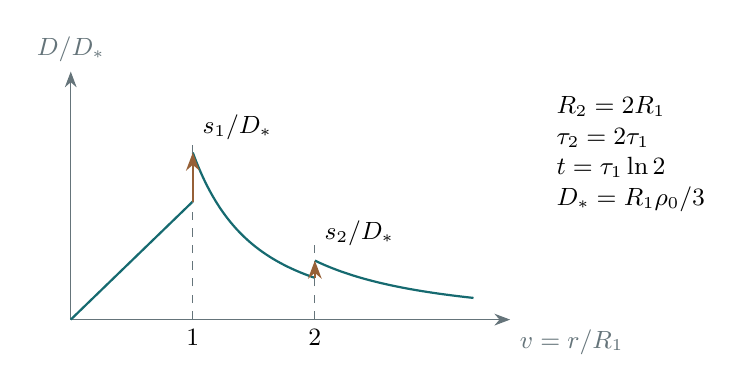
\begin{tikzpicture}[x=1.55cm,y=3cm,font=\small]
\draw[axis](0,0)--(3.6,0)node[below right]{$v=r/R_1$};\draw[axis](0,0)--(0,1.05)node[above]{$D/D_*$};
\draw[traj](0,0)--(1,.5);
\draw[traj,domain=1:2,samples=65,variable=\t]plot(\t,{sqrt(.5)/(\t*\t)});
\draw[traj,domain=2:3.3,samples=65,variable=\t]plot(\t,{1/(\t*\t)});
\draw[guide](1,0)--(1,.76);\draw[guide](2,0)--(2,.35);
\draw[force](1,.5)--(1,.707107);\draw[force](2,.176777)--(2,.25);
\node[above right]at(1,.72){$s_1/D_*$};\node[above right]at(2,.27){$s_2/D_*$};
\node[below]at(1,0){$1$};\node[below]at(2,0){$2$};
\node[right,align=left]at(3.9,.7){$R_2=2R_1$\\$\tau_2=2\tau_1$\\$t=\tau_1\ln2$\\$D_*=R_1\rho_0/3$};
\end{tikzpicture}
\figcaption{解图电4.4C　三段电位移的一个实际时刻。径向向外为正，两个向上跳变分别等于两界面的自由面电荷，外部场不随时间改变。}
\end{minipage}\end{center}

解图电4.4C用同一时刻的三段D显示边界跳变。代入差指数后，中间段化为
\[
D=\frac{R_1^3\rho_0}{3r^2}e^{-t/\tau_2},
\]
其时间常数只剩$\tau_2$。
在$R_1$处右减左为$s_1$；在$R_2$处外减内为$s_2$。最外段与t无关，因为任何自由电荷都未穿过外边界；它也保证当内部场最终归零时，球外电场仍存在。
外表面的面电荷增长率等于内侧流向表面的电流密度：
\[
\dot s_2=j(R_2^-)=\frac{Q_0e^{-t/\tau_2}}{4\pi R_2^2\tau_2}.
\]
积分后与总电荷法一致。
两界面上的电荷分别由两侧的径向电流之差积累。把面密度乘相应球面积得到两面的电荷量，与内球的体电荷相加为初始总电荷。


\Needspace{8\baselineskip}

\pdfbookmark[3]{关键洞察}{q4-h5}

\subsection*{关键洞察}

$R_2$ 内的总自由电荷按 $\tau_2$ 衰减，内球体电荷按 $\tau_1$ 衰减，二者之差就是内界面电荷。外层送电荷较快时内界面可暂带负电；三项代数和始终固定。

\Needspace{8\baselineskip}

\pdfbookmark[3]{易错点}{q4-h6}

\subsection*{易错点}

两种介质各用本侧的 $\varepsilon_i$ 把 $D$ 换成 $E$，各用 $\tau_i$ 把 $D$ 换成 $j$。电位移连续只在对应界面自由电荷为零时成立。内外两面总电荷需分别乘 $4\pi R_1^2$ 和 $4\pi R_2^2$。

\Needspace{8\baselineskip}

\pdfbookmark[3]{课堂讲解建议}{q4-h7}

\subsection*{课堂讲解建议}

先沿解图电4.4C标三个取样高斯面，分别指出每个高斯面包进了哪些自由电荷。再到解图电4.4A让学生预测两个材料时标交换后界面的电流差符号，随后用变图电4.4V2算峰值。

将外层换成理想绝缘体后，请学生在变图电4.4V3解释电荷停在哪一面。用变图电4.4V8辨认快、慢两个过程，并指出球壳内场变小与内球内场消失分别发生在哪个时段。

\Needspace{18\baselineskip}
\pdfbookmark[3]{变式训练}{q4-h8}

\subsection*{变式训练}

\begin{enumerate}
\item 若 $\tau_1=\tau_2=\tau$，解图电4.4A的初始条件 $D_{1+}=D_{1-}$ 也给 $j_{1+}=j_{1-}$。之后 $\dot s_1=-s_1/\tau$，故 $s_1=0$。变图电4.4V1的两支 $D$ 箭头始终同长，$E_+/E_-=\varepsilon_1/\varepsilon_2$，所以电场仍可跃变。没有内界面电荷时，$s_2=R_1^3\rho_0(1-e^{-t/\tau})/(3R_2^2)$。
\begin{center}\begin{minipage}{.98\linewidth}\centering
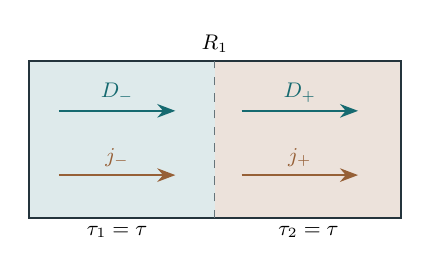
\begin{tikzpicture}[scale=.85,transform shape]
\fill[accent!14](0,0)rectangle(2.78,2.35);
\fill[warm!18](2.78,0)rectangle(5.56,2.35);
\draw[object](0,0)rectangle(5.56,2.35);
\draw[guide](2.78,0)--(2.78,2.35);
\foreach \x/\z in {.45/{-},3.18/{+}}{
\draw[motion](\x,1.60)--({\x+1.74},1.60)node[midway,above]{$D_{\z}$};
\draw[force](\x,.64)--({\x+1.74},.64)node[midway,above]{$j_{\z}$};}
\node[below]at(1.32,0){$\tau_1=\tau$};\node[below]at(4.18,0){$\tau_2=\tau$};
\node[above]at(2.78,2.35){$R_1$};
\end{tikzpicture}
\figcaption{变图电4.4V1\quad 相等的弛豫时间使内界面同时满足电位移和传导电流连续}
\end{minipage}\end{center}
\item 写 $c=R_1\rho_0/3$。求导给 $\dot s_1=c(e^{-t/\tau_1}/\tau_1-e^{-t/\tau_2}/\tau_2)$，令其为零，取对数得
\[
t_*=\frac{\tau_1\tau_2}{\tau_2-\tau_1}\ln\frac{\tau_2}{\tau_1}.
\]
变图电4.4V2取 $\tau_2=2\tau_1$，由 $t_*=2\tau_1\ln2$ 得 $e^{-t_*/\tau_2}=1/2$、$e^{-t_*/\tau_1}=1/4$，故 $s_1(t_*)=c/4$。若交换 $\tau_1,\tau_2$，时刻保持而峰值反号，成为负极小。
\begin{center}\begin{minipage}{.98\linewidth}\centering
\begin{tikzpicture}[scale=.85,transform shape]
\begin{scope}[x=1.29cm,y=3.65cm]
\draw[axis](0,0)--(4.93,0)node[right]{$t/\min(\tau_1,\tau_2)$};
\draw[axis](0,-0.36)--(0,0.43)node[above]{$s_1/c$};
\draw[traj,domain=0:4.7,samples=88]plot(\x,{exp(-\x/2)-exp(-\x)});
\draw[object,dashed,domain=0:4.7,samples=88]plot(\x,{exp(-\x)-exp(-\x/2)});
\draw[guide](1.386294,-.25)--(1.386294,.25);
\fill[accent](1.386294,.25)circle(1.55pt) (1.386294,-.25)circle(1.55pt);
\node[above]at(1.386294,.25){$+1/4$};
\node[below]at(1.386294,-.25){$-1/4$};
\node[right]at(2.7,.25){$\tau_2=2\tau_1$};
\node[right]at(2.62,-.26){交换时标};
\end{scope}
\end{tikzpicture}
\figcaption{变图电4.4V2\quad 内界面电荷的极值对应流入与流出两侧电流相等}
\end{minipage}\end{center}
\item 若外层理想绝缘，$\sigma_2=0$，所以 $\dot s_1=j_{1-}=ce^{-t/\tau_1}/\tau_1$。积分给 $s_1=c(1-e^{-t/\tau_1})$，外界面始终 $s_2=0$。变图电4.4V3中内球减去的体电荷都转移到内界面。球壳内电位移为 $Q_0/(4\pi r^2)$，而它的导电电流因 $\sigma_2=0$ 为零。
\begin{center}\begin{minipage}{.98\linewidth}\centering
\begin{tikzpicture}[scale=.85,transform shape]
\begin{scope}[x=1.29cm,y=2.73cm]
\draw[axis](0,0)--(4.93,0)node[right]{$t/\tau_1$};
\draw[axis](0,0)--(0,1.21)node[above]{$Q/Q_0$};
\draw[object,dashed,domain=0:4.65,samples=88]plot(\x,{exp(-\x)});
\draw[traj,domain=0:4.65,samples=88]plot(\x,{1-exp(-\x)});
\draw[guide](0,1)--(4.65,1);
\node[left]at(0,1){$1$};
\node[above]at(2.95,.94){内界面 $Q_{s_1}/Q_0$};
\node[above]at(2.62,.075){内球 $Q_{\text{体}}/Q_0$};
\node[below]at(2.6,0){外界面为零};
\end{scope}
\end{tikzpicture}
\figcaption{变图电4.4V3\quad 外层绝缘时，内球的自由电荷积到内界面后停止外迁}
\end{minipage}\end{center}
\item 反转初始体电荷 $\rho_0\to-\rho_0$。场方程和界面守恒都是线性的，$E,D,j,\rho_e,s_1,s_2$ 均反号，$\tau_i$ 保持。变图电4.4V4在 $\tau_2=2\tau_1$ 下，以正量 $|Q_0|$ 为标度画外表面电荷。正、负两组曲线互为镜像；两组三项代数和分别为 $+|Q_0|,-|Q_0|$。
\begin{center}\begin{minipage}{.98\linewidth}\centering
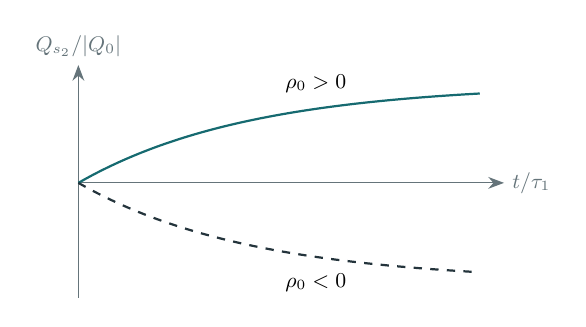
\begin{tikzpicture}[scale=.85,transform shape]
\begin{scope}[x=1.29cm,y=1.48cm]
\draw[axis](0,0)--(4.93,0)node[right]{$t/\tau_1$};
\draw[axis](0,-1.16)--(0,1.19)node[above]{$Q_{s_2}/|Q_0|$};
\draw[traj,domain=0:4.65,samples=88]plot(\x,{1-exp(-\x/2)});
\draw[object,dashed,domain=0:4.65,samples=88]plot(\x,{-(1-exp(-\x/2))});
\node[above]at(2.75,.83){$\rho_0>0$};
\node[below]at(2.75,-.83){$\rho_0<0$};
\end{scope}
\end{tikzpicture}
\figcaption{变图电4.4V4\quad 改变初始自由电荷符号，外表面电荷的时间曲线关于零线镜像}
\end{minipage}\end{center}
\item 若内界面已有 $s_{10}$，设 $c=R_1\rho_0/3$，仍用相同的内界面驱动方程，但初值变为 $s_1(0)=s_{10}$。乘积分因子得到
\[
s_1(t)=(s_{10}+c)e^{-t/\tau_2}-ce^{-t/\tau_1}.
\]
总自由电荷为 $Q'_0=Q_0+4\pi R_1^2s_{10}$，所以 $s_2=Q'_0(1-e^{-t/\tau_2})/(4\pi R_2^2)$。变图电4.4V5取 $Q'_0=0$，内球和内面的异号电荷等量衰减，外面一直不积电。
\begin{center}\begin{minipage}{.98\linewidth}\centering
\begin{tikzpicture}[scale=.85,transform shape]
\begin{scope}[x=1.29cm,y=1.49cm]
\draw[axis](0,0)--(4.93,0)node[right]{$t/\tau_1$};
\draw[axis](0,-1.14)--(0,1.19)node[above]{$Q/(4\pi R_1^2c)$};
\draw[traj,domain=0:4.65,samples=88]plot(\x,{exp(-\x)});
\draw[object,dashed,domain=0:4.65,samples=88]plot(\x,{-exp(-\x)});
\node[above]at(1.91,.37){$Q_{\text{体}}/Q_0$};
\node[below]at(1.92,-.39){$Q_{s_1}/Q_0$};
\node[above]at(3.63,.053){$Q_{s_2}=0$};
\end{scope}
\end{tikzpicture}
\figcaption{变图电4.4V5\quad 初始总自由电荷为零时，两种内部电荷等量衰减}
\end{minipage}\end{center}
\item 球外高斯面恒包围同一总自由电荷，故 $E(r)=Q_0/(4\pi\varepsilon_0 r^2)$ 与时间无关，$\partial_tD=0$。外部真空内传导电流也为零。变图电4.4V6标出球内两层的 $j$ 和 $\partial_tD$：由 $D$ 各按本层时标衰减，$\partial_tD=-D/\tau_i=-j$。因此在任一界面，总电流的径向分量两侧相等；传导电流的跳量由面电荷变化率平衡。
\begin{center}\begin{minipage}{.98\linewidth}\centering
\begin{tikzpicture}[scale=.85,transform shape]
\fill[accent!17](0,0)rectangle(5.96,2.67);
\fill[white](3.66,0)rectangle(5.96,2.67);
\draw[object](0,0)rectangle(5.96,2.67);
\draw[guide](3.66,0)--(3.66,2.67);
\draw[guide](1.81,0)--(1.81,2.67);
\foreach \a/\b/\i in {.27/1.52/1,2.13/3.34/2}{
\draw[motion](\a,1.85)--(\b,1.85)node[midway,above]{$j_{\i}$};
\draw[force](\b,.78)--(\a,.78)node[midway,above]{$\partial_tD_{\i}$};}
\node[below]at(1.81,0){$R_1$};
\node at(4.83,1.59){外部 $j=0$};
\node at(4.83,.87){$\partial_t D=0$};
\node[below]at(3.66,0){$R_2$};
\end{tikzpicture}
\figcaption{变图电4.4V6\quad 球内传导与位移电流反向相消，球外的电通量恒定}
\end{minipage}\end{center}
\item 令 $R_2\to2R_2$，保持 $R_1$ 及物性。内界面方程与内球弛豫保持，两个系统共有的球壳区域的 $D,j$ 也相同。变图电4.4V7把两个外球并列；同一时刻的外表面总电荷都是 $Q_0(1-e^{-t/\tau_2})$，较大球的面积增为四倍，故 $s_2$ 降为四分之一。
\begin{center}\begin{minipage}{.98\linewidth}\centering
\begin{tikzpicture}[scale=.85,transform shape]
\draw[object](0,0)circle(.82);
\draw[object](4.21,0)circle(1.64);
\draw[guide](0,0)circle(.52) (4.21,0)circle(.52);
\draw[object,<->](0,0)--(0:.82)node[midway,above]{$R_2$};
\begin{scope}[shift={(4.21,0)}]
\draw[object,<->](0,0)--(0:1.64)node[midway,above]{$2R_2$};
\end{scope}
\node[below]at(0,-.89){面积 $4\pi R_2^2$};
\node[below]at(4.21,-1.68){面积 $4(4\pi R_2^2)$};
\end{tikzpicture}
\figcaption{变图电4.4V7\quad 外球面积变为四倍时，守恒给同一总电荷，面密度降为四分之一}
\end{minipage}\end{center}
\item 若 $\tau_2\ll\tau_1$，可在变图电4.4V8的对数时间轴上分辨两个过程。当 $\tau_2\ll t\ll\tau_1$，$e^{-t/\tau_2}$ 近零而 $e^{-t/\tau_1}$ 近1，故 $Q_{\text{体}}\simeq Q_0$、$Q_{s_1}\simeq-Q_0$、$Q_{s_2}\simeq Q_0$。内界面的负电荷使壳内 $D$ 很小，内球中的正电荷仍按较慢时标衰减，随后内界面负电荷才逐渐消失。
\begin{center}\begin{minipage}{.98\linewidth}\centering
\begin{tikzpicture}[scale=.85,transform shape]
\begin{scope}[x=1.5cm,y=1.23cm]
\draw[axis](-3,0)--(1.14,0)node[right]{$\log_{10}(t/\tau_1)$};
\draw[axis](-3,-1.16)--(-3,1.25)node[above]{$Q/Q_0$};
\draw[traj,domain=-3:1,samples=92]plot(\x,{exp(-pow(10,\x))});
\draw[object,dashed,domain=-3:1,samples=92]plot(\x,{1-exp(-100*pow(10,\x))});
\draw[warm,thick,domain=-3:1,samples=92]plot(\x,{exp(-100*pow(10,\x))-exp(-pow(10,\x))});
\draw[guide](-2,-.95)--(-2,1) (0,-.95)--(0,1);
\node[below]at(-2,0){$-2$};\node[below]at(0,0){$0$};
\node[above]at(-1.20,1){$Q_{s_2}$};
\node[above]at(-.31,.58){$Q_{\text{体}}$};
\node[below]at(-.91,-.897){$Q_{s_1}$};
\end{scope}
\end{tikzpicture}
\figcaption{变图电4.4V8\quad 取 $\tau_2=0.01\tau_1$，两竖线分别对应 $t=\tau_2$、$t=\tau_1$}
\end{minipage}\end{center}
\end{enumerate}

\Needspace{13\baselineskip}

\pdfbookmark[2]{第 5 题 无碰撞双组分载流子的纵向小振动}{q5}

\section*{第 5 题\quad 无碰撞双组分载流子的纵向小振动}\label{q:5}

一均匀柱形介质的介电常量为$\varepsilon$，含正、负载流子，质量分别为$m_+,m_-$，电荷为$q_+>0,q_-<0$。平衡时两组分电荷体密度为$+\rho_0,-\rho_0$。温度足够低，可忽略热运动和碰撞阻尼。沿柱轴$x$有微小纵向扰动，使两组分发生电荷分离。在线性近似下证明该电荷分离模为简谐振动并求角频率；说明整体共同平移与此模的区别。

\begin{center}\begin{minipage}{.98\linewidth}\centering
\begin{tikzpicture}[scale=.9,transform shape]

\draw[object](0,0) rectangle(7,2.1);\foreach \x in {.5,1.5,2.5,3.5,4.5,5.5,6.5}{\node[color=accent] at(\x,1.4){$+$};\node[color=warm] at(\x,.6){$-$};}
\draw[axis](0,-.6)--(7.6,-.6) node[right]{$x$};\node[above] at(3.5,2.1){平衡：$+\rho_0,-\rho_0$};

\end{tikzpicture}
\figcaption{图电4.5\quad 两组分在同一介质中互相穿插，平衡时宏观电中性。}
\end{minipage}\end{center}

\Needspace{8\baselineskip}

\pdfbookmark[3]{题型定位}{q5-h0}

\subsection*{题型定位}

冷双流体的线性纵向小振动。用连续性和高斯定律闭合电荷扰动方程，再以相对坐标与质心分开解释振动和平移。

\Needspace{8\baselineskip}

\pdfbookmark[3]{知识点}{q5-h1}

\subsection*{知识点}

一阶电流为 $\rho_0(v_+-v_-)$，由平衡电荷密度乘一阶速度。动力学中的荷质比带电荷符号。连续性和 高斯定律给 $\ddot\rho=-\omega_p^2\rho$；一维平面端部的均匀分离给 $E=-\rho_0\xi/\varepsilon$。相对惯性由约化质量密度 $\mu_r$ 决定。

\Needspace{8\baselineskip}

\pdfbookmark[3]{物理图像}{q5-h2}

\subsection*{物理图像}

解图电4.5A的相对位移在端面或局部造成净电荷和恢复场，共同位移则保持两组分重叠。解图电4.5B中两组分反相，轻组分振幅更大。解图电4.5C中位移极大时电场能最大，过平衡位置时相对动能最大。

\Needspace{8\baselineskip}

\pdfbookmark[3]{解题入口}{q5-h3}

\subsection*{解题入口}

在薄片上写流入减流出和电通量差。对 $j$ 求时间导数并代入两种粒子加速度，再对连续性方程求导，得到只含净电荷的方程。讨论均匀相对位移时另用端面恢复场，取没有外加总电流的条件。之后以质量密度加权重建两组分的位移。

\Needspace{18\baselineskip}
\pdfbookmark[3]{标准解法}{q5-h4}

\subsection*{标准解法}

图电4.5中两组分稍作相反位移时，端部或局部密度起伏产生恢复电场。保留到扰动的一阶，电流密度为
\[
j=\rho_+v_++\rho_-v_-\simeq\rho_0(v_+-v_-).
\]
其中$\delta\rho_\pm v_\pm$为二阶小量，在线性化时略去。用解图电4.5A的薄片控制体写出
\[
\partial_t\rho=-\partial_xj,\qquad \partial_xE=\rho/\varepsilon,
\qquad m_\pm\partial_tv_\pm=q_\pm E.
\]

\begin{center}\begin{minipage}{.98\linewidth}\centering
\begin{tikzpicture}[scale=.9,transform shape]

\node[anchor=west] at(0,2.8){电荷分离模};\draw[guide](1,0)--(1,2.3);
\draw[motion](1,1.8)--(2.3,1.8) node[right]{$\xi_+$};\draw[force](1,1)--(.2,1) node[left]{$\xi_-$};
\draw[axis](2.1,.15)--(.2,.15) node[midway,below]{$E=-\rho_0\xi/\varepsilon$};
\node[anchor=west] at(5,2.8){共同平移};\draw[guide](5.5,.7)--(5.5,2.3);
\draw[motion](5.5,1.8)--(7,1.8) node[right]{$\xi_+$};\draw[force](5.5,1)--(7,1) node[right]{$\xi_-$};
\node at(6.5,0){$\xi=0,\quad\ddot X=0$};
\draw[object](3,-2.5) rectangle(4,-1.5);\draw[motion](1.6,-2)--(2.8,-2) node[midway,above]{$j(x)$};\draw[motion](4.2,-2)--(5.5,-2) node[midway,above]{$j(x+\dd x)$};
\draw[<->](3,-2.9)--(4,-2.9) node[midway,below]{$\dd x$};\draw[axis](5.8,-2)--(7.2,-2) node[right]{$x$};

\end{tikzpicture}
\figcaption{解图电4.5A\quad 相对位移产生恢复电场；共同平移不产生电荷分离，是不同的自由模。}
\end{minipage}\end{center}

对电流式求时间导数，再用两个动力学方程：
\[
\partial_tj=\rho_0\left(\frac{q_+}{m_+}-\frac{q_-}{m_-}\right)E.
\]
对连续性方程再求一次时间导数，并对上式作空间导数，得到
\[
\partial_t^2\rho=-\rho_0\left(\frac{q_+}{m_+}-\frac{q_-}{m_-}\right)\partial_xE
=-\frac{\rho_0}{\varepsilon}\left(\frac{q_+}{m_+}-\frac{q_-}{m_-}\right)\rho.
\]
所以电荷分离的角频率为
\[
\boxed{\omega_p=\sqrt{\frac{\rho_0}{\varepsilon}\left(\frac{q_+}{m_+}-\frac{q_-}{m_-}\right)}}.
\]
$q_-<0$，括号实际是两个正贡献之和，因此 $\omega_p^2>0$，密度扰动随时间作振动。密度扰动可写为$\rho(x,t)=A(x)\cos\omega_pt+B(x)\sin\omega_pt$，幅函数还需满足初始及边界条件。

解图电4.5A的两端面给出均匀位移的恢复场。令 $\xi=\xi_+-\xi_-$。取两组分重合时的场为零，$\xi>0$ 使右端出现正面电荷 $\rho_0\xi$，左端出现负面电荷 $-\rho_0\xi$。在一维平面模型中，两端面的场叠加为 $E=-\rho_0\xi/\varepsilon$，于是
\[
\ddot\xi=\left(\frac{q_+}{m_+}-\frac{q_-}{m_-}\right)E=-\omega_p^2\xi.
\]
该电场方向使正载流子向后、负载流子向前，减小分离。两质量密度分别为$\mu_\pm=\rho_0m_\pm/|q_\pm|$，总质心满足
\[
(\mu_++\mu_-)\ddot X=(\rho_0-\rho_0)E=0.
\]
所以共同平移满足 $X=X_0+V_0t$。相对振动叠加在这一匀速运动上；用随质心移动的坐标描述时，两组分各以同一频率振动。


解图电4.5A下方薄片还能把局部方程的符号写得更明确。截面积S、长度$\dd x$内的电荷变化为
\[
[\rho(x,t+\dd t)-\rho(x,t)]S\dd x=[j(x,t)-j(x+\dd x,t)]S\dd t.
\]
流入大于流出才使正电荷增加；约去共同因子并取极限，才得到$\partial_t\rho=-\partial_xj$。
同一薄片的左右电通量差为$[E(x+\dd x)-E(x)]S=\rho S\dd x/\varepsilon$，给出高斯定律。两式均以向右为正，负组分的符号已计入带符号电荷密度。

求导时的完整电流表达式是
\[
\partial_tj=\rho_+\partial_tv_++\rho_-\partial_tv_-+
(\partial_t\rho_+)v_++(\partial_t\rho_-)v_-.
\]
平衡速度为零，$v_\pm,\delta\rho_\pm$均为一阶扰动，最后两项为二阶；前两项中的$\rho_\pm$可取$\pm\rho_0$，其修正再乘一阶加速度也是二阶。
动力学中完整的物质加速度还可含$v_\pm\partial_xv_\pm$，它在同一线性近似下亦为二阶。这里忽略碰撞、压强和热运动，才得到所用的冷流体方程。

若沿电场路线计算，连续性与高斯定律只能先推出
\[
\partial_x(\varepsilon\partial_tE+j)=0,\qquad
\varepsilon\partial_tE+j=C(t).
\]
函数 $C(t)$ 是空间均匀的总电流密度，由端部与外部驱动条件确定。
在没有外加总电流的平面电荷分离模中取$C=0$，再求时间导数得到$\varepsilon\ddot E=-\dot j$，结合动力学也给$\ddot E+\omega_p^2E=0$。
对于沿轴整体均匀的相对位移，体内$\rho$可为零，恢复场由两端面电荷产生，在这一均匀模中，由端面带电量及几何条件确定场幅。
均匀相对位移的端部恢复场采用平面近似，局部体电荷的振动采用一维纵向方程。若端部场有显著的横向变化，均匀位移的恢复力需按实际几何求出。
\begin{center}\begin{minipage}{.97\linewidth}\centering
\begin{tikzpicture}[x=.85cm,y=2.2cm,font=\small]
\draw[axis](0,0)--(6.7,0)node[below right]{$\theta=\omega_pt$};\draw[axis](0,-1)--(0,1.1)node[above]{$\xi_\pm/\xi_0$};
\draw[traj,domain=0:6.283185,samples=120,variable=\t]plot(\t,{.2*cos(\t r)});
\draw[thick,warm,domain=0:6.283185,samples=120,variable=\t]plot(\t,{-.8*cos(\t r)});
\node[below]at(1.570796,-1.03){$\pi/2$};\node[below]at(3.141593,-1.03){$\pi$};\node[below]at(6.283185,-1.03){$2\pi$};
\node[left]at(0,.2){$1/5$};\node[left]at(0,-.8){$-4/5$};
\node[right,accent]at(7,.1){$\xi_+$};\node[right,warm]at(7,-.45){$\xi_-$};
\node[above]at(3.4,1.1){$\mu_+=4\mu_-,\quad X=0$};
\end{tikzpicture}
\figcaption{解图电4.5B　质量密度不等时的纯相对振动。两组分位移反相、幅度不同，质量加权中心保持不动；相对位移幅值为$\xi_0$。}
\end{minipage}\end{center}

解图电4.5B将两个粒子群的位移和质心分开。对纯相对模取$X=0$，联立$\mu_+\xi_++\mu_-\xi_-=0$与$\xi=\xi_+-\xi_-$，得
\[
\xi_+=\frac{\mu_-}{\mu_++\mu_-}\xi,\qquad
\xi_-=-\frac{\mu_+}{\mu_++\mu_-}\xi.
\]
所以两组分反相，但只有质量密度相同时振幅才相等。B图取$\mu_+=4\mu_-$，正组分振幅为相对振幅的1/5，负组分为4/5；按质量密度加权的中心在每一时刻都不动。
对一般初值，两式右边各加同一个 $X=X_0+V_0t$。取两式之差便消去共同平移，余下电荷分离位移 $\xi$。
\begin{center}\begin{minipage}{.97\linewidth}\centering
\begin{tikzpicture}[x=.85cm,y=2.5cm,font=\small]
\draw[axis](0,0)--(6.7,0)node[below right]{$\theta=\omega_pt$};\draw[axis](0,0)--(0,1.3)node[above]{能量比例};
\draw[traj,domain=0:6.283185,samples=140,variable=\t]plot(\t,{cos(\t r)^2});
\draw[thick,warm,domain=0:6.283185,samples=140,variable=\t]plot(\t,{sin(\t r)^2});
\draw[guide](0,1)--(6.3,1);\node[left]at(0,1){$1$};
\node[below]at(1.570796,0){$\pi/2$};\node[below]at(3.141593,0){$\pi$};\node[below]at(6.283185,0){$2\pi$};
\node[right,accent]at(7,1){$u_E/u_0$};\node[right,warm]at(7,.55){$u_K/u_0$};\node[right]at(7,.1){$u_E+u_K=u_0$};
\end{tikzpicture}
\figcaption{解图电4.5C　以初速度为零的纯相对模为例，场能与相对动能周期交换；频率相同的两组分共同承担相对动能。}
\end{minipage}\end{center}

解图电4.5C显示相对动能和电场能随时间的交换。定义约化质量密度$\mu_r=\mu_+\mu_-/(\mu_++\mu_-)$，则
\[
u_K=\frac12\mu_r\dot\xi^2,\qquad
u_E=\frac12\varepsilon E^2=\frac{\rho_0^2}{2\varepsilon}\xi^2,\qquad
\omega_p^2=\frac{\rho_0^2}{\varepsilon\mu_r}.
\]
由$1/\mu_r=1/\mu_++1/\mu_-$代回，最后一式正好等于两个荷质比之和给出的频率平方。
取$\xi=\xi_0\cos\omega_pt$，令$u_0=\rho_0^2\xi_0^2/(2\varepsilon)$，便有$u_E/u_0=\cos^2\omega_pt$、$u_K/u_0=\sin^2\omega_pt$。
场对两组分做功的总功率$jE=\rho_0\dot\xi E=-\dd u_E/\dd t$，与动能增加相抵，电场减少的能量恰成为相对动能。
共同平移若存在，还需加常量$\tfrac12(\mu_++\mu_-)V_0^2$，它不参与C图的周期能量交换。


\Needspace{8\baselineskip}

\pdfbookmark[3]{关键洞察}{q5-h5}

\subsection*{关键洞察}

纯相对模的场能由分离距离决定，约化质量密度决定惯性；共同移动不改变分离距离，其质心保持匀速。沿轴均匀错位可只在端部带电，体密度方程给体内局部扰动，均匀场由端部条件决定。

\Needspace{8\baselineskip}

\pdfbookmark[3]{易错点}{q5-h6}

\subsection*{易错点}

负载流子电荷取带符号值 $q_-<0$。一阶电流保留平衡密度乘速度，密度扰动乘速度属二阶。将 $\partial_x(\varepsilon\dot E+j)=0$ 沿轴积分后保留空间均匀的 $C(t)$，用外电路或端部条件定值。反相振幅按质量密度反比分配。

\Needspace{8\baselineskip}

\pdfbookmark[3]{课堂讲解建议}{q5-h7}

\subsection*{课堂讲解建议}

先让学生沿解图电4.5A的轴画出正、负两组分相对及共同位移后的端面，标恢复场对两者的力向。用变图电4.5V2固定背景，再用变图电4.5V3让两边都可运动，比较同一个分离量对应的相对加速度。

取解图电4.5B的质量密度比 $4:1$，先令学生由质心关系算速度幅值，再用变图电4.5V7求两边动能份额。最后用变图电4.5V8指出成对内摩擦改变的是相对动能与场能的交换。

\Needspace{18\baselineskip}
\pdfbookmark[3]{变式训练}{q5-h8}

\subsection*{变式训练}

\begin{enumerate}
\item 令 $q_+=+e,q_-=-e$，由中性条件两种载流子的平衡数密度同为 $n$。于是
\[
\omega_p^2=\frac{ne^2}{\varepsilon}\left(\frac1{m_+}+\frac1{m_-}\right).
\]
若两个质量都乘 $\lambda$，括号变为原值的 $1/\lambda$。变图电4.5V1画归一化频率 $\lambda^{-1/2}$，故两质量同时加倍给 $\omega_p/\omega_{p0}=1/\sqrt2$。若只改变其中一种质量，则只改变式中对应的一项。
\begin{center}\begin{minipage}{.98\linewidth}\centering
\begin{tikzpicture}[scale=.85,transform shape]
\begin{scope}[x=1.7cm,y=2.77cm]
\draw[axis](.83,0)--(4.34,0)node[right]{$\lambda$};
\draw[axis](.83,0)--(.83,1.18)node[above]{$\omega_p/\omega_{p0}$};
\draw[traj,domain=1:4,samples=90]plot(\x,{1/sqrt(\x)});
\draw[guide](2,0)--(2,.707107)--(.83,.707107);
\fill[accent](2,.707107)circle(1.55pt);
\node[left]at(.83,.707107){$1/\sqrt2$};\node[below]at(2,0){$2$};
\end{scope}
\end{tikzpicture}
\figcaption{变图电4.5V1\quad 同时增加两种载流子质量，恢复场不变，振动惯性增大}
\end{minipage}\end{center}
\item 当 $m_+\to\infty$，正载流子可作为固定背景。变图电4.5V2取负组分向右移 $\xi_->0$，左右端分别露出正、负电荷，故 $E=\rho_0\xi_-/\varepsilon$ 指向右。负载流子受到向左的力，方程为 $m_-\ddot\xi_-=q_-E$，所以
\[
\omega_p^2=\frac{\rho_0|q_-|}{\varepsilon m_-}.
\]
在一般表达式中只需令 $q_+/m_+\to0$，同样得到这一频率。
\begin{center}\begin{minipage}{.98\linewidth}\centering
\begin{tikzpicture}[scale=.85,transform shape]
\fill[accent!12](0,0)rectangle(4.63,1.61);
\draw[object](0,0)rectangle(4.63,1.61);
\fill[warm!16](.82,.2)rectangle(5.45,1.42);
\draw[traj](.82,.2)rectangle(5.45,1.42);
\foreach \y in {.34,.79,1.24}{\node at(.38,\y){$+$};\node at(5.0,\y){$-$};}
\draw[motion](1.91,.96)--(3.48,.96)node[midway,above]{$E$};
\draw[force](3.48,.39)--(1.91,.39)node[midway,below]{$q_-E$};
\draw[object,<->](4.63,1.85)--(5.45,1.85)node[midway,above]{$\xi_-$};
\end{tikzpicture}
\figcaption{变图电4.5V2\quad 负组分移开固定的正背景后，端面场使负载流子回到重合位置}
\end{minipage}\end{center}
\item 若 $|q_+|=|q_-|$ 且 $m_+=m_-$，两种质量密度均为 $\mu$。在质心系，变图电4.5V3中两个位移分别为 $+\xi/2,-\xi/2$，其差仍为 $\xi$，恢复场仍为 $-\rho_0\xi/\varepsilon$。约化质量密度由固定一组分时的 $\mu$ 降为 $\mu/2$，所以两组分都可运动时的频率为固定一组分时的 $\sqrt2$ 倍。
\begin{center}\begin{minipage}{.98\linewidth}\centering
\begin{tikzpicture}[scale=.85,transform shape]
\draw[axis](-3.04,0)--(3.07,0)node[right]{$x$};
\draw[guide](0,-.83)--(0,1.43)node[above]{质心};
\filldraw[fill=warm!24,draw=ink](-1.58,0)circle(.25)node{$-$};
\filldraw[fill=accent!24,draw=ink](1.58,0)circle(.25)node{$+$};
\draw[motion](0,.51)--(-1.58,.51)node[midway,above]{$-\xi/2$};
\draw[motion](0,.51)--(1.58,.51)node[midway,above]{$+\xi/2$};
\draw[object,<->](-1.58,-.58)--(1.58,-.58)node[midway,below]{$\xi$};
\end{tikzpicture}
\figcaption{变图电4.5V3\quad 相同质量密度时，两组分在质心两侧等幅反向运动}
\end{minipage}\end{center}
\item 若质心有速度 $v_c$，取 $X=X_0+v_ct$，两组分的位移是 $X+\mu_-\xi/(\mu_++\mu_-)$ 和 $X-\mu_+\xi/(\mu_++\mu_-)$。变图电4.5V4取相同质量密度，虚线是匀速质心，另两曲线与它的偏差反号，差值仍作谐振。共同平移的两项电流 $\rho_0v_c$ 与 $-\rho_0v_c$ 相消，净传导电流为 $\rho_0\dot\xi$。
\begin{center}\begin{minipage}{.98\linewidth}\centering
\begin{tikzpicture}[scale=.85,transform shape]
\begin{scope}[x=0.97cm,y=1.17cm]
\draw[axis](0,0)--(6.68,0)node[right]{$\omega_pt$};
\draw[axis](0,-.71)--(0,2.82)node[above]{位移};
\draw[guide,domain=0:6.3,samples=90]plot(\x,{.31*\x});
\draw[traj,domain=0:6.3,samples=90]plot(\x,{.31*\x+.53*cos(deg(\x))});
\draw[object,dashed,domain=0:6.3,samples=90]plot(\x,{.31*\x-.53*cos(deg(\x))});
\node[right]at(6.32,2.47){$\xi_+$};
\node[right]at(6.32,1.97){$X$};
\node[right]at(6.32,1.41){$\xi_-$};
\end{scope}
\end{tikzpicture}
\figcaption{变图电4.5V4\quad 实验室坐标下，两组分都随同一质心匀速移动，并叠加相反的振动}
\end{minipage}\end{center}
\item 设 $\xi_0=\xi_{+0}-\xi_{-0}$、$v_{r0}=v_{+0}-v_{-0}$，则
\[
\xi(t)=\xi_0\cos\omega_pt+\frac{v_{r0}}{\omega_p}\sin\omega_pt .
\]
变图电4.5V5中的两相坐标 $(\xi,\dot\xi/\omega_p)$ 在尺度一致时绕中心顺时针转动。初态定下幅值 $\sqrt{\xi_0^2+(v_{r0}/\omega_p)^2}$ 和相位。用两种质量密度加权求 $X_0,V_0$，再将 $X_0+V_0t$ 加至两组分的相对坐标即可。
\begin{center}\begin{minipage}{.98\linewidth}\centering
\begin{tikzpicture}[scale=.85,transform shape]
\draw[axis](-2.21,0)--(2.4,0)node[right]{$\xi$};
\draw[axis](0,-1.85)--(0,1.99)node[above]{$\dot\xi/\omega_p$};
\draw[traj](0,0)circle(1.48);
\draw[guide](0,0)--(30:1.48);
\draw[guide](30:1.48)--(1.28172,0) (30:1.48)--(0,.74);
\fill[accent](30:1.48)circle(1.7pt)node[above right]{初态};
\draw[motion](30:1.48)arc[start angle=30,end angle=-48,radius=1.48];
\node[below right]at(1.28,0){$\xi_0$};
\node[left]at(0,.74){$v_{r0}/\omega_p$};
\end{tikzpicture}
\figcaption{变图电4.5V5\quad 给定相对初位移和初速度后，相轨迹的半径和起点随之确定}
\end{minipage}\end{center}
\item 将介电常量改为 $4\varepsilon$，在相同相对位移下，端面自由电荷由两组分相对位移决定，场强变为四分之一。单位体积的场能对相对位移的二阶导数由 $\rho_0^2/\varepsilon$ 变为原来的四分之一，而约化质量密度相同。于是 $\omega\to\omega_p/2$。变图电4.5V6给相同初位移、零初速度，较大介电常量下经过原本的一个周期时，系统只走完半个周期。
\begin{center}\begin{minipage}{.98\linewidth}\centering
\begin{tikzpicture}[scale=.85,transform shape]
\begin{scope}[x=0.99cm,y=1.35cm]
\draw[axis](0,0)--(6.6,0)node[right]{$\omega_pt$};
\draw[axis](0,-1.21)--(0,1.23)node[above]{$\xi/\xi_0$};
\draw[object,dashed,domain=0:6.3,samples=90]plot(\x,{cos(deg(\x))});
\draw[traj,domain=0:6.3,samples=90]plot(\x,{cos(deg(\x)/2)});
\draw[guide](6.28319,-1)--(6.28319,1);
\node[below right]at(6.28,0){$2\pi$};
\node[left]at(0,1){$1$};
\node[above left]at(6.23,1){$\varepsilon$};\node[below left]at(6.23,-1){$4\varepsilon$};
\end{scope}
\end{tikzpicture}
\figcaption{变图电4.5V6\quad 同一端面电荷的恢复场减弱，介电常量增为四倍时周期加倍}
\end{minipage}\end{center}
\item 纯相对振动振幅为 $A$ 时，最大相对速度为 $\omega_p A$。两组分的速度分别用 $+\mu_-/(\mu_++\mu_-)$ 和 $-\mu_+/(\mu_++\mu_-)$ 乘 $\dot\xi$，故
\[
u_{K+}:u_{K-}=\mu_-:\mu_+,\qquad
u_{K+}+u_{K-}=\tfrac12\mu_r\dot\xi^2.
\]
变图电4.5V7采用 $\mu_+=4\mu_-$。两组分动量反向等大，轻组分的速度幅值为重组分四倍，承担 $4/5$ 的相对动能。
\begin{center}\begin{minipage}{.98\linewidth}\centering
\begin{tikzpicture}[scale=.85,transform shape]
\draw[axis](0,0)--(6.36,0)node[right]{相对动能};
\fill[warm!53](0,.64)rectangle(1.17,1.43);
\fill[accent!48](1.17,.64)rectangle(5.85,1.43);
\draw[object](0,.64)rectangle(5.85,1.43);
\node at(.585,1.02){$1/5$};
\node at(3.51,1.02){$4/5$};
\node[above]at(.585,1.47){正组分};
\node[above]at(3.51,1.47){负组分};
\draw[guide](1.17,0)--(1.17,.64) (5.85,0)--(5.85,.64);
\node[below]at(5.85,0){$\tfrac12\mu_r\dot\xi^2$};
\end{tikzpicture}
\figcaption{变图电4.5V7\quad 轻组分速度较大，在质心固定时承担更多相对动能}
\end{minipage}\end{center}
\item 给正组分的单位体积内摩擦力为 $-\gamma\dot\xi$，给负组分的力相反。两动力学方程相加后内摩擦相消，质心仍自由平移。两加速度相减，整理成
\[
\mu_r\ddot\xi+\gamma\dot\xi+\frac{\rho_0^2}{\varepsilon}\xi=0,\qquad
\dot u=-\gamma\dot\xi^2.
\]
令 $\beta=\gamma/(2\mu_r)$。$\beta<\omega_p$ 时为衰减振荡，角频率 $\sqrt{\omega_p^2-\beta^2}$；临界及过阻尼解均无周期振荡。变图电4.5V8取 $\beta=0.2\omega_p$、零初速度，曲线的幅值随时间减小，正负包络按 $e^{-\beta t}$ 缩小。
\begin{center}\begin{minipage}{.98\linewidth}\centering
\begin{tikzpicture}[scale=.85,transform shape]
\begin{scope}[x=0.54cm,y=1.43cm]
\draw[axis](0,0)--(12.4,0)node[right]{$\omega_pt$};
\draw[axis](0,-1.18)--(0,1.27)node[above]{$\xi/\xi_0$};
\draw[traj,domain=0:12,samples=90]plot(\x,{exp(-.2*\x)*(cos(deg(sqrt(.96)*\x))+.2/sqrt(.96)*sin(deg(sqrt(.96)*\x)))});
\draw[guide,domain=0:12,samples=90]plot(\x,{exp(-.2*\x)/sqrt(.96)});
\draw[guide,domain=0:12,samples=90]plot(\x,{-exp(-.2*\x)/sqrt(.96)});
\node[above]at(5.3,.43){上包络};
\node[below]at(5.4,-.43){下包络};
\end{scope}
\end{tikzpicture}
\figcaption{变图电4.5V8\quad 成对的内摩擦从相对模耗散能量，质心运动保持自由}
\end{minipage}\end{center}
\end{enumerate}

\Needspace{13\baselineskip}

\pdfbookmark[2]{第 6 题 增加两个相同电阻能否保持端口电阻}{q6}

\section*{第 6 题\quad 增加两个相同电阻能否保持端口电阻}\label{q:6}

有限个阻值均为$r>0$的电阻构成二端网络，等效电阻为$R>0$。把该网络视为只可使用其两个端口的元件，在端口外以串、并联方式接入另两个阻值为$r$的电阻，两个新增电阻均须有效接入。能否使新的二端等效电阻仍等于$R$？

\begin{center}\begin{minipage}{.98\linewidth}\centering
\begin{tikzpicture}[scale=.9,transform shape]

\draw[object](0,0)--(1,0);\draw[object](1,-.6) rectangle(3,.6);\node at(2,0){有限网络$R$};\draw[object](3,0)--(4,0);
\fill(0,0) circle(2pt) node[left]{$A$};\fill(4,0) circle(2pt) node[right]{$B$};
\draw[object](5.5,-.35) rectangle(6.5,.35);\node at(6,0){$r$};\draw[object](8,-.35) rectangle(9,.35);\node at(8.5,0){$r$};
\node at(7.2,1){待接入的两个电阻};\node at(2,-1.2){仅使用$A,B$两个端口};

\end{tikzpicture}
\figcaption{图电4.6\quad 既有网络作为二端元件，新增电阻仅在端口之外连接。}
\end{minipage}\end{center}

\Needspace{8\baselineskip}

\pdfbookmark[3]{题型定位}{q6-h0}

\subsection*{题型定位}

三元件串并联分类结合有限电阻网络的有理性。先求可能保持阻值的比值，再用整数节点方程判断这两个比值能否由有限同值电阻实现。

\Needspace{8\baselineskip}

\pdfbookmark[3]{知识点}{q6-h1}

\subsection*{知识点}

最外层连接为串联或并联，内层的另外两个元件也只可能串联或并联。交换两只同值新增电阻后共六类。有限网络中用 $r$ 和端电压归一化，节点线性方程有整数系数，所以端口电导和电阻的归一化值都是有理数。

\Needspace{8\baselineskip}

\pdfbookmark[3]{物理图像}{q6-h2}

\subsection*{物理图像}

解图电4.6A画出六种接法。两种混合接法有可能用一个步骤的增量抵消另一步的减量，在解图电4.6C中对应增量曲线的零点。解图电4.6B演示有限网络如何从节点电势和端口电流得到有理阻值。

\Needspace{8\baselineskip}

\pdfbookmark[3]{解题入口}{q6-h3}

\subsection*{解题入口}

把既有网络整体记为 $R$，按最外串联或并联给六类排序。排除单调增大、单调减小的四种后，对余下两种列出 $R_{\rm new}=R$。求得正根，再用固定端电势的节点方程说明有限网络的 $R/r$ 为有理数。

\Needspace{18\baselineskip}
\pdfbookmark[3]{标准解法}{q6-h4}

\subsection*{标准解法}

图电4.6把既有网络作为电阻为$R$的二端元件。三个元件构成的串并联网络，交换两个相同的$r$后只有解图电4.6A中的六类；图中仅使用既有网络的两个端口，两个新增电阻均承载非零电流。

\begin{center}\begin{minipage}{.98\linewidth}\centering
\begin{tikzpicture}[scale=.95,transform shape]

\begin{scope}[yshift=3.5cm]
\draw[object](0,0)--(3,0);\foreach \x/\s in {.5/R,1.5/r,2.5/r}{\node[draw,fill=white] at(\x,0){$\s$};}\node at(1.5,-.7){(1) $R+r+r$};
\draw[object](5,0)--(6,0)--(6,.5)--(8,.5)--(8,0)--(8,-.5)--(6,-.5)--(6,0);\node[draw,fill=white] at(5.5,0){$R$};\node[draw,fill=white] at(7,.5){$r$};\node[draw,fill=white] at(7,-.5){$r$};\node at(6.5,-1.15){(2) $R+(r\parallel r)$};
\end{scope}
\draw[object](0,0)--(0,1)--(3,1)--(3,0)--(3,-1)--(0,-1)--(0,0)--(3,0);\foreach \y/\s in {1/R,0/r,-1/r}{\node[draw,fill=white] at(1.5,\y){$\s$};}\node at(1.5,-1.65){(3) $R\parallel r\parallel r$};
\draw[object](5,0)--(5,.5)--(7,.5)--(7,-.5)--(5,-.5)--(5,0) (7,0)--(9,0);\node[draw,fill=white] at(6,.5){$R$};\node[draw,fill=white] at(6,-.5){$r$};\node[draw,fill=white] at(8,0){$r$};\node at(6.8,-1.65){(4) $(R\parallel r)+r$};
\begin{scope}[yshift=-4cm]
\draw[object](0,0)--(0,.5)--(3,.5)--(3,-.5)--(0,-.5)--cycle;\node[draw,fill=white] at(.8,.5){$R$};\node[draw,fill=white] at(2.2,.5){$r$};\node[draw,fill=white] at(1.5,-.5){$r$};\node at(1.5,-1.2){(5) $(R+r)\parallel r$};
\draw[object](5,0)--(5,.5)--(8,.5)--(8,-.5)--(5,-.5)--cycle;\node[draw,fill=white] at(6.5,.5){$R$};\node[draw,fill=white] at(5.8,-.5){$r$};\node[draw,fill=white] at(7.2,-.5){$r$};\node at(6.5,-1.2){(6) $R\parallel(r+r)$};
\end{scope}

\end{tikzpicture}
\figcaption{解图电4.6A\quad 六种串并联连接按两个相同$r$电阻的交换对称去重；各式对应同排电路。}
\end{minipage}\end{center}

按解图电4.6A从左至右、从上至下计算：
\[
\begin{aligned}
R_1&=R+2r,&R_2&=R+\frac r2,&R_3&=\frac{Rr}{2R+r},\\
R_4&=r+\frac{Rr}{R+r},&R_5&=\frac{r(R+r)}{R+2r},&R_6&=\frac{2Rr}{R+2r}.
\end{aligned}
\]
第1、2类在 $R$ 外增加串联电阻，所以结果较大。第3、6类在 $R$ 两端增加并联通路，所以结果较小。对第四种令$R_4=R$，乘$R+r$并整理：
\[
r(R+r)+Rr=R(R+r)\quad\Longrightarrow\quad R^2-Rr-r^2=0,
\]
所以正根为$R/r=(1+\sqrt5)/2$。第五种则给
\[
r(R+r)=R(R+2r)\quad\Longrightarrow\quad R^2+Rr-r^2=0,
\]
正根为$R/r=(\sqrt5-1)/2$。这两个条件本身允许正电阻，却都要求无理数比值。

还须使用“$R$由有限个相同电阻组成”的条件。把各节点电势以端口电压归一化，基尔霍夫方程的系数均为整数，消元所得节点电势和端口电流系数均为有理数。因此任何这样的有限网络都有
\[
\frac Rr\in\mathbb Q.
\]
这与两种根式条件矛盾，故\boxed{\text{在上述端口串并联条件下不能保持阻值不变。}}

若解除有限性，某些无限梯形网络恰有黄金比阻值，添加一节后可以保持不变；若允许进入已有网络的内部等势点，则还可能加上无电流支路。本题的六种连接以既有网络有限、只开放两个端口以及新增支路有效为条件。

\begin{center}\begin{minipage}{.97\linewidth}\centering
\begin{tikzpicture}[scale=.9,font=\small]
\draw[object](0,0)--(2,2)--(4,0)--cycle;
\node[draw,fill=white]at(1,1){$r$};\node[draw,fill=white]at(3,1){$r$};\node[draw,fill=white]at(2,0){$r$};
\fill(0,0)circle(1.5pt)node[left]{$A:v_A=1$};\fill(4,0)circle(1.5pt)node[right]{$B:v_B=0$};
\fill(2,2)circle(1.5pt)node[above]{$P:v_P=1/2$};
\node[align=left]at(8,1.1){$2v_P=1+0$\\$Ir/\Delta U=1+(1-v_P)=3/2$\\$R/r=2/3$};
\end{tikzpicture}
\figcaption{解图电4.6B　有限相同电阻网络的一个节点计算示例。单位端电压下先求内部有理电势，再求有理端口电导。}
\end{minipage}\end{center}

解图电4.6B以一个有限三角网络说明节点法的两步。令$v=V/\Delta U$，内部P点满足$(v_P-1)+(v_P-0)=0$，得$v_P=1/2$。
A端电流包括直接支路$\Delta U/r$与经P支路$\Delta U/(2r)$，所以$Ir/\Delta U=3/2$、$R/r=2/3$。
把解图电4.6B的内部节点方程推广到任意有限网络。对每个内部节点列$\sum_j(v_i-v_j)=0$，多条相同电阻边只使整数系数相加。
固定两端电势后，与端口相连部分的约化节点矩阵可逆；克拉默法则或有限高斯消元给有理节点电势。再把端口各支路的有理电流相加，得到非零有理电导，其倒数仍为有理数。
\begin{center}\begin{minipage}{.97\linewidth}\centering
\begin{tikzpicture}[x=2cm,y=1.7cm,font=\small]
\draw[axis](0,0)--(2.5,0)node[below right]{$x=R/r$};\draw[axis](0,0)--(0,2.6)node[above]{$R_{\text{新}}/r$};
\draw[guide](0,0)--(2.3,2.3);
\draw[traj,domain=0:2.3,samples=80,variable=\t]plot(\t,{1+\t/(1+\t)});
\draw[thick,warm,domain=0:2.3,samples=80,variable=\t]plot(\t,{(\t+1)/(\t+2)});
\fill(1.618034,1.618034)circle(1.5pt);\fill(.618034,.618034)circle(1.5pt);
\node[above left]at(1.618034,1.618034){$\varphi$};\node[below right]at(.618034,.618034){$1/\varphi$};
\node[right,accent]at(2.7,2){第(4)类：$1+x/(1+x)$};\node[right,warm]at(2.7,1.2){第(5)类：$(1+x)/(2+x)$};
\node[right]at(2.7,.45){虚线：保持条件$y=x$};
\end{tikzpicture}
\figcaption{解图电4.6C　两种混合连接的实际函数与保持直线。两处交点的横坐标是两种接法的正固定点。}
\end{minipage}\end{center}

解图电4.6C比较两种混合连接的增量。
第(4)类先并联再串联，增减可以抵消；第(5)类也有正的固定点。令$x=R/r$，两种增量分别为
\[
\frac{R_4-R}{r}=\frac{1+x-x^2}{1+x},\qquad
\frac{R_5-R}{r}=\frac{1-x-x^2}{2+x}.
\]
分母在$x>0$始终为正，故交点两侧确有增减方向变化。有限同值电阻网络的 $x$ 是有理数，因而实际可取点位于这两个无理数的两侧。
六类枚举的完整性来自三个二端元件的串并联构造：最外一步若为串联，内侧剩两元件可串或并；最外一步若为并联，内侧可并或串。再按哪个位置放R及两个r可交换去重，恰得解图电4.6A所列六类。


\Needspace{8\baselineskip}

\pdfbookmark[3]{关键洞察}{q6-h5}

\subsection*{关键洞察}

两种混合接法的正根互为倒数。有限同值网络的端口阻值能随构造逼近根，却始终是有理数；无限梯形网络的极限能取无理固定点。

\Needspace{8\baselineskip}

\pdfbookmark[3]{易错点}{q6-h6}

\subsection*{易错点}

新增电阻的接点仅在既有网络端口外。六类按拓扑和函数区分，个别初始阻值相同只会使部分结果恰巧重合。有限一般网络的有理性来自节点矩阵，即使遇到不能逐步化成串并联的桥式结构也可用此法。

\Needspace{8\baselineskip}

\pdfbookmark[3]{课堂讲解建议}{q6-h7}

\subsection*{课堂讲解建议}

先让学生看解图电4.6A给第4、5类各写两步等效式，再沿解图电4.6C找到两处零点，说明为什么正根确实能补偿阻值。随后回到解图电4.6B，用一个归一化内部电势算端口电流，再把这一方法推广到一般整数节点方程。

对照变图电4.6V5和V6，前者改变两只新增电阻的比值，能构造精确补偿；后者反复加入同值元件，在有限步中逐渐接近黄金比。

\Needspace{18\baselineskip}
\pdfbookmark[3]{变式训练}{q6-h8}

\subsection*{变式训练}

\begin{enumerate}
\item 若 $R$ 可独立取任意正值，可把其设为 $\varphi r$，$\varphi=(1+\sqrt5)/2$。变图电4.6V1先将 $R$ 和 $r$ 并联，再与另一只 $r$ 串联。由 $\varphi^2=\varphi+1$ 得
\[
\frac{R_{\rm new}}r=1+\frac{\varphi}{1+\varphi}=1+\frac1\varphi=\varphi.
\]
两个新增支路均通电，这给出该串并联结构的正固定点。
\begin{center}\begin{minipage}{.98\linewidth}\centering
\begin{tikzpicture}[scale=.85,transform shape]
\draw[object](0.0000,0.0000)--(1.1000,0.0000);
\draw[object](1.1000,0.6600)--(1.1000,-0.6600);
\draw[object](4.1000,0.6600)--(4.1000,-0.6600);
\draw[object](1.1000,0.6600)--(2.1000,0.6600);
\draw[object](3.1000,0.6600)--(4.1000,0.6600);
\draw[object](2.1000,0.7900)--(3.1000,0.7900)--(3.1000,0.5300)--(2.1000,0.5300)--cycle;
\node[above,inner sep=1pt]at(2.6000,0.9500){$\varphi r$};
\draw[object](1.1000,-0.6600)--(2.1000,-0.6600);
\draw[object](3.1000,-0.6600)--(4.1000,-0.6600);
\draw[object](2.1000,-0.5300)--(3.1000,-0.5300)--(3.1000,-0.7900)--(2.1000,-0.7900)--cycle;
\node[above,inner sep=1pt]at(2.6000,-0.3700){$r$};
\draw[object](4.1000,0.0000)--(4.7100,0.0000);
\draw[object](5.7100,0.0000)--(6.3200,0.0000);
\draw[object](4.7100,0.1300)--(5.7100,0.1300)--(5.7100,-0.1300)--(4.7100,-0.1300)--cycle;
\node[above,inner sep=1pt]at(5.2100,0.2900){$r$};
\fill[ink](0.0000,0.0000)circle(1.6pt)node[left]{A};
\fill[ink](6.3200,0.0000)circle(1.6pt)node[right]{B};
\fill[ink](1.1000,0.0000)circle(1.6pt)node[left]{};
\fill[ink](4.1000,0.0000)circle(1.6pt)node[left]{};
\end{tikzpicture}
\figcaption{变图电4.6V1\quad 先并联后串联时，黄金比给出端口阻值不变的构造}
\end{minipage}\end{center}
\item 变图电4.6V2先将 $R$ 与一只 $r$ 串联，再把另一只 $r$ 跨接在两端。令 $\psi=1/\varphi=(\sqrt5-1)/2$，取 $R=\psi r$。由于 $\psi^2+\psi=1$，有
\[
R_{\rm new}/r=\frac{\psi+1}{\psi+2}=\psi.
\]
两条固定点方程的正根互为倒数，分别对应图中的两种内外串并联次序。
\begin{center}\begin{minipage}{.98\linewidth}\centering
\begin{tikzpicture}[scale=.85,transform shape]
\draw[object](0.0000,0.0000)--(1.1000,0.0000);
\draw[object](4.1000,0.0000)--(6.3200,0.0000);
\draw[object](1.1000,0.6600)--(1.1000,-0.6600);
\draw[object](4.1000,0.6600)--(4.1000,-0.6600);
\draw[object](1.1000,0.6600)--(1.4366,0.6600);
\draw[object](2.2934,0.6600)--(2.6300,0.6600);
\draw[object](1.4366,0.7900)--(2.2934,0.7900)--(2.2934,0.5300)--(1.4366,0.5300)--cycle;
\node[above,inner sep=1pt]at(1.8650,0.8700){$\psi r$};
\draw[object](2.6300,0.6600)--(2.9534,0.6600);
\draw[object](3.7766,0.6600)--(4.1000,0.6600);
\draw[object](2.9534,0.7900)--(3.7766,0.7900)--(3.7766,0.5300)--(2.9534,0.5300)--cycle;
\node[above,inner sep=1pt]at(3.3650,0.8700){$r$};
\draw[object](1.1000,-0.6600)--(2.1000,-0.6600);
\draw[object](3.1000,-0.6600)--(4.1000,-0.6600);
\draw[object](2.1000,-0.5300)--(3.1000,-0.5300)--(3.1000,-0.7900)--(2.1000,-0.7900)--cycle;
\node[below,inner sep=1pt]at(2.6000,-0.9400){$r$};
\fill[ink](0.0000,0.0000)circle(1.6pt)node[left]{A};
\fill[ink](6.3200,0.0000)circle(1.6pt)node[right]{B};
\fill[ink](1.1000,0.0000)circle(1.6pt)node[left]{};
\fill[ink](4.1000,0.0000)circle(1.6pt)node[left]{};
\end{tikzpicture}
\figcaption{变图电4.6V2\quad 先串联后并联时，保持阻值所需的比值是黄金比的倒数}
\end{minipage}\end{center}
\item 若既有网络只是 $R=r$，在六个连接式中令 $x=R/r=1$，得到 $R_{\rm new}/r$ 依次为
\[
 3,\quad \frac32,\quad \frac13,\quad \frac32,\quad \frac23,\quad \frac23.
\]
变图电4.6V3的水平线表示接入前的 $R/r=1$。第2、4类的柱高同为 $3/2$，第5、6类同为 $2/3$；将 $x$ 改离1后，分别按六个连接式计算。
\begin{center}\begin{minipage}{.98\linewidth}\centering
\begin{tikzpicture}[scale=.85,transform shape]
\draw[axis](0,0)--(6.51,0)node[right]{接法};
\draw[axis](0,0)--(0,3.36)node[above]{$R_{\rm new}/r$};
\foreach \x/\h/\i in {1/3/1,2/1.5/2,3/.333333/3,4/1.5/4,5/.666667/5,6/.666667/6}{
\fill[accent!37]({\x-.29},0)rectangle({\x+.29},\h);
\node[below]at(\x,0){$\i$};}
\draw[object,dashed](0,1)--(6.33,1);
\node[left]at(0,1){$1$};\node[left]at(0,3){$3$};
\end{tikzpicture}
\figcaption{变图电4.6V3\quad 既有网络只有一只电阻时，六种接法均改变阻值}
\end{minipage}\end{center}
\item 变图电4.6V4上行中新增的电阻一端悬空，端点守恒给零电流；下行新增电阻跨接在一段理想导线上，电压为零，也无电流。若两个新增电阻均按这样的方式连接，端口电流仍为 $\Delta U/R$。题设要求两个新增电阻在端口加压时都有非零电流。允许接入内部节点时，则按新的节点电势和支路电流判断。
\begin{center}\begin{minipage}{.98\linewidth}\centering
\begin{tikzpicture}[scale=.85,transform shape]
\draw[object](0,1.54)--(1.48,1.54)--(1.48,2.46)--(2.11,2.46) (3.14,2.46)--(3.82,2.46);
\draw[object](2.11,2.31)rectangle(3.14,2.61);
\node[above]at(2.62,2.61){新增 $r$};
\filldraw[fill=white,draw=ink](3.82,2.46)circle(1.9pt);
\draw[object](1.48,1.54)--(2.11,1.54) (3.14,1.54)--(5.2,1.54);
\draw[object](2.11,1.39)rectangle(3.14,1.69);
\node[below]at(2.62,1.39){$R$};
\node[right]at(5.22,1.54){悬空，$I_r=0$};
\draw[object](0,0)--(2.11,0) (3.14,0)--(5.2,0);
\draw[object](2.11,-.14)rectangle(3.14,.14);
\node[above]at(2.62,.14){$R$};
\draw[object](3.46,0)--(3.46,-.92)--(3.76,-.92) (4.46,-.92)--(4.76,-.92)--(4.76,0);
\draw[object](3.76,-1.04)rectangle(4.46,-.80);
\node[below]at(4.11,-1.04){新增 $r$};
\node[right]at(5.22,0){短接，$U_r=0$};
\end{tikzpicture}
\figcaption{变图电4.6V4\quad 悬空和跨接理想导线的新增支路均不承担电流}
\end{minipage}\end{center}
\item 若两只新增电阻可分别取 $2r,r$，取既有网络 $R=2r$，可由两只 $r$ 串成。变图电4.6V5将既有的 $2r$ 与新增的 $2r$ 并联，得到 $r$，再串新增的 $r$，结果为 $2r$。设端口电压为 $\Delta U>0$，经过串联支路的电流 $\Delta U/(2r)$ 在两只相同的并联支路各分一半，两个新增支路都有效。
\begin{center}\begin{minipage}{.98\linewidth}\centering
\begin{tikzpicture}[scale=.85,transform shape]
\draw[object](0.0000,0.0000)--(1.1000,0.0000);
\draw[object](1.1000,0.6600)--(1.1000,-0.6600);
\draw[object](4.1000,0.6600)--(4.1000,-0.6600);
\draw[object](1.1000,0.6600)--(2.1000,0.6600);
\draw[object](3.1000,0.6600)--(4.1000,0.6600);
\draw[object](2.1000,0.7900)--(3.1000,0.7900)--(3.1000,0.5300)--(2.1000,0.5300)--cycle;
\node[above,inner sep=1pt]at(2.6000,0.9500){$R=2r$};
\draw[object](1.1000,-0.6600)--(2.1000,-0.6600);
\draw[object](3.1000,-0.6600)--(4.1000,-0.6600);
\draw[object](2.1000,-0.5300)--(3.1000,-0.5300)--(3.1000,-0.7900)--(2.1000,-0.7900)--cycle;
\node[above,inner sep=1pt]at(2.6000,-0.3700){新增 $2r$};
\draw[object](4.1000,0.0000)--(4.7100,0.0000);
\draw[object](5.7100,0.0000)--(6.3200,0.0000);
\draw[object](4.7100,0.1300)--(5.7100,0.1300)--(5.7100,-0.1300)--(4.7100,-0.1300)--cycle;
\node[above,inner sep=1pt]at(5.2100,0.2900){新增 $r$};
\fill[ink](0.0000,0.0000)circle(1.6pt)node[left]{A};
\fill[ink](6.3200,0.0000)circle(1.6pt)node[right]{B};
\fill[ink](1.1000,0.0000)circle(1.6pt)node[left]{};
\fill[ink](4.1000,0.0000)circle(1.6pt)node[left]{};
\end{tikzpicture}
\figcaption{变图电4.6V5\quad 两只新增电阻采用不同阻值时，可用有理数阻值精确补偿}
\end{minipage}\end{center}
\item 连续使用第4类连接，写成 $x_{n+1}=1+x_n/(1+x_n)$、$x_0=1$。变图电4.6V6依次给 $1,3/2,8/5,21/13,55/34$，再趋向 $\varphi$。从递推式减去固定点式得
\[
x_{n+1}-\varphi=\frac{x_n-\varphi}{(1+x_n)(1+\varphi)}.
\]
分母大于1，误差同号且幅值逐步缩小。本例始终从下方接近黄金比；任意有限步的端口阻值比仍可写成整数之比。
\begin{center}\begin{minipage}{.98\linewidth}\centering
\begin{tikzpicture}[scale=.85,transform shape]
\begin{scope}[x=1.15cm,y=4.64cm]
\draw[axis](0,.88)--(5.18,.88)node[right]{$n$};
\draw[axis](0,.88)--(0,1.78)node[above]{$x_n$};
\draw[guide](0,1.6180340)--(4.93,1.6180340)node[right]{$\varphi$};
\draw[traj]plot coordinates {(0,1) (1,1.5) (2,1.6) (3,1.6153846) (4,1.6176471)};
\foreach \x/\y in {0/1,1/1.5,2/1.6,3/1.6153846,4/1.6176471}{
\fill[accent](\x,\y)circle(1.6pt);
\node[below]at(\x,.88){$\x$};}
\node[below right]at(1,1.5){$3/2$};
\end{scope}
\end{tikzpicture}
\figcaption{变图电4.6V6\quad 重复接入同一节，有限步骤的有理阻值从同一侧靠近无理固定点}
\end{minipage}\end{center}
\item 令 $x=R/r$。变图电4.6V7画两种混合接法的归一化增量 $(1+x-x^2)/(1+x)$ 和 $(1-x-x^2)/(2+x)$。前者在 $x=\varphi$ 由正转负，后者在 $x=1/\varphi$ 由正转负。取 $x=2/3$，则第4类增量为 $11/15>0$，第5类为 $-1/24<0$。相同初始阻值下，两种接法可给相反的变化方向。
\begin{center}\begin{minipage}{.98\linewidth}\centering
\begin{tikzpicture}[scale=.85,transform shape]
\begin{scope}[x=2.67cm,y=2.18cm]
\draw[axis](0,0)--(2.48,0)node[right]{$x$};
\draw[axis](0,-1.23)--(0,1.24)node[above]{增量除以 $r$};
\draw[traj,domain=0:2.29,samples=83]plot(\x,{(1+\x-(\x)^2)/(1+\x)});
\draw[object,dashed,domain=0:2.18,samples=83]plot(\x,{(1-\x-(\x)^2)/(2+\x)});
\fill[accent](1.61803399,0)circle(1.55pt) (0.61803399,0)circle(1.55pt);
\node[below right]at(1.61803399,0){$\varphi$};
\node[below left]at(0.61803399,0){$1/\varphi$};
\node[above]at(1.34,.31){第4类};
\node[below]at(1.34,-.65){第5类};
\end{scope}
\end{tikzpicture}
\figcaption{变图电4.6V7\quad 两种混合连接的增量分别在各自的固定点改变符号}
\end{minipage}\end{center}
\item 若有限网络各支路的阻值为 $r$ 的正有理倍数，归一化电导仍为有理数。变图电4.6V8以不平衡桥为例，令端口归一化电势为1和0，内部两点为 $u,v$。支路标值给
\[
\tfrac72u-2v=1,\qquad -2u+\tfrac{17}6v=\tfrac13 .
\]
解得 $u=42/71,v=38/71$，端口归一化电流为 $1-u+(1-v)/3=40/71$，故 $R/r=71/40$。一般的有限有理节点矩阵给同样的有理性，两无理固定点仍无法取得。
\begin{center}\begin{minipage}{.98\linewidth}\centering
\begin{tikzpicture}[scale=.85,transform shape]
\draw[object](0.0000,0.0000)--(1.0492,0.5036);
\draw[object](1.9508,0.9364)--(3.0000,1.4400);
\draw[object](0.9930,0.6208)--(1.8945,1.0536)--(2.0070,0.8192)--(1.1055,0.3864)--cycle;
\node[above,inner sep=1pt]at(1.3745,0.9814){$r$};
\draw[object](3.0000,1.4400)--(4.0492,0.9364);
\draw[object](4.9508,0.5036)--(6.0000,0.0000);
\draw[object](4.1055,1.0536)--(5.0070,0.6208)--(4.8945,0.3864)--(3.9930,0.8192)--cycle;
\node[above,inner sep=1pt]at(4.6255,0.9814){$2r$};
\draw[object](0.0000,0.0000)--(1.0492,-0.5036);
\draw[object](1.9508,-0.9364)--(3.0000,-1.4400);
\draw[object](1.1055,-0.3864)--(2.0070,-0.8192)--(1.8945,-1.0536)--(0.9930,-0.6208)--cycle;
\node[below,inner sep=1pt]at(1.3659,-0.9995){$3r$};
\draw[object](3.0000,-1.4400)--(4.0492,-0.9364);
\draw[object](4.9508,-0.5036)--(6.0000,0.0000);
\draw[object](3.9930,-0.8192)--(4.8945,-0.3864)--(5.0070,-0.6208)--(4.1055,-1.0536)--cycle;
\node[below,inner sep=1pt]at(4.6341,-0.9995){$2r$};
\draw[object](3.0000,1.4400)--(3.0000,0.5000);
\draw[object](3.0000,-0.5000)--(3.0000,-1.4400);
\draw[object](3.1300,0.5000)--(3.1300,-0.5000)--(2.8700,-0.5000)--(2.8700,0.5000)--cycle;
\node[right,inner sep=1pt]at(3.3100,0.0000){$r/2$};
\fill[ink](0.0000,0.0000)circle(1.6pt)node[left]{$1$};
\fill[ink](6.0000,0.0000)circle(1.6pt)node[right]{$0$};
\fill[ink](3.0000,1.4400)circle(1.6pt)node[above]{$u$};
\fill[ink](3.0000,-1.4400)circle(1.6pt)node[below]{$v$};
\end{tikzpicture}
\figcaption{变图电4.6V8\quad 有理支路阻值的桥式网络也可用有理节点方程求端口电阻}
\end{minipage}\end{center}
\end{enumerate}

\Needspace{13\baselineskip}

\pdfbookmark[2]{第 7 题 由三个端口测量反推六只电阻}{q7}

\section*{第 7 题\quad 由三个端口测量反推六只电阻}\label{q:7}

图电4.7中，$a,b,c$分别为端点$X,Y,Z$的外接电阻，内部三角形的$X$侧至$Y$侧、$Y$侧至$Z$侧、$Z$侧至$X$侧分别为$f,d,e$。六只电阻恰为$1,2,3,4,5,6\,\Omega$各一只。第三端悬空时测得
\[
R_{XY}=7\frac3{13}\,\Omega,\quad R_{YZ}=10\frac1{13}\,\Omega,\quad R_{ZX}=6\frac9{13}\,\Omega.
\]
求$a,b,c,d,e,f$各自的阻值。

\begin{center}\begin{minipage}{.98\linewidth}\centering
\begin{tikzpicture}[scale=.9,transform shape]

\coordinate(X) at(0,2.5);\coordinate(Y) at(6,2.5);\coordinate(Z) at(3,-2);
\coordinate(P) at(1.5,1.3);\coordinate(Q) at(4.5,1.3);\coordinate(T) at(3,-.7);
\draw[object](X)--(P) (Y)--(Q) (Z)--(T) (P)--(Q)--(T)--cycle;
\foreach \p/\s in {X/X,Y/Y}{\fill(\p) circle(1.5pt) node[above]{$\s$};}
\fill(Z)circle(1.5pt)node[below]{$Z$};
\node[fill=white] at(.75,1.9){$a$};\node[fill=white] at(5.25,1.9){$b$};\node[fill=white] at(3,-1.35){$c$};
\node[fill=white] at(3,1.3){$f$};\node[fill=white] at(3.75,.3){$d$};\node[fill=white] at(2.25,.3){$e$};

\end{tikzpicture}
\figcaption{图电4.7\quad 外接三只电阻与内部三角形的标签固定，第三端在各次测量时悬空。}
\end{minipage}\end{center}

\Needspace{8\baselineskip}

\pdfbookmark[3]{题型定位}{q7-h0}

\subsection*{题型定位}

由三个二端测量识别六条支路。用不可约分母约束内部三角形的电阻和，再用测量的分数部分确定内侧标号、整数部分恢复外接阻值。

\Needspace{8\baselineskip}

\pdfbookmark[3]{知识点}{q7-h1}

\subsection*{知识点}

第三端悬空时，对应外接电阻中电流为零，三角形仍可绕行分流。测量中分数项的最简分母整除内三角形的电阻和。三角形转成星形后，每个内星臂是该节点相邻两内边的乘积除以三边和。

\Needspace{8\baselineskip}

\pdfbookmark[3]{物理图像}{q7-h2}

\subsection*{物理图像}

解图电4.7A的 $T_f,T_d,T_e$ 对应三次测量各自看到的直接内边及其绕行通路。解图电4.7B把外接电阻和内星臂合为总星臂。解图电4.7C的 $c$ 端断开，$d,e$ 串起来的通路仍参与分流。

\Needspace{8\baselineskip}

\pdfbookmark[3]{解题入口}{q7-h3}

\subsection*{解题入口}

为三个端口分别写外接两臂与内部并联项。用最简分母13确定三角形内边和，再算两个可取三元组的分数部分完成配对。扣除内部项后，按三个两两和求外接电阻。

\Needspace{18\baselineskip}
\pdfbookmark[3]{标准解法}{q7-h4}

\subsection*{标准解法}

测 $X,Y$ 时，图电4.7的外侧电阻 $a,b$ 在被测通路上，$c$ 支路悬空。内部一边为 $f$，另一边经 $e,d$ 串联，两条内部通路并联。令$D=d+e+f$，三个方程为
\[
R_{XY}=a+b+\frac{f(e+d)}D,\quad
R_{YZ}=b+c+\frac{d(f+e)}D,\quad
R_{ZX}=c+a+\frac{e(d+f)}D.
\]

\begin{center}\begin{minipage}{.98\linewidth}\centering
\begin{tikzpicture}[scale=.9,transform shape]

\draw[object](0,0)--(1,0)--(1,1)--(5,1)--(5,0)--(6,0) (1,0)--(1,-1)--(5,-1)--(5,0);
\node[draw,fill=white] at(.5,0){$a$};\node[draw,fill=white] at(5.5,0){$b$};
\node[draw,fill=white] at(3,1){$f$};\node[draw,fill=white] at(2,-1){$e$};\node[draw,fill=white] at(4,-1){$d$};
\node[left] at(0,0){$X$};\node[right] at(6,0){$Y$};\node at(3,-1.8){$T_f=f\parallel(e+d)$};
\node[align=left] at(8.5,.4){$T_f=42/13$\\$T_d=40/13$\\$T_e=22/13$};

\end{tikzpicture}
\figcaption{解图电4.7A\quad 测量$X,Y$时内部两条路径并联；右侧列出确定后的三个内部等效项（单位为欧姆）。}
\end{minipage}\end{center}

解图电4.7A把这些分式分别记为$T_f,T_d,T_e$。六只电阻均取整数欧姆，而测量含不可约分母13，所以这些分式的分母$D$必须含因子13。三只不同电阻之和在6至15之间，故
\[
D=13\,\Omega,\qquad\{d,e,f\}=\{3,4,6\}\ \text{或}\ \{2,5,6\}.
\]
若取$\{3,4,6\}$，三个分式为$30/13,36/13,42/13$，小数部分为$4/13,10/13,3/13$，不能与测量中的$3/13,1/13,9/13$匹配。因此只剩$\{2,5,6\}$。

这一组中，各阻值与其分式的对应为
\[
2\longmapsto\frac{22}{13}=1\frac9{13},\quad
5\longmapsto\frac{40}{13}=3\frac1{13},\quad
6\longmapsto\frac{42}{13}=3\frac3{13}.
\]
由测量的小数部分逐项对应，得$e=2\,\Omega,d=5\,\Omega,f=6\,\Omega$。从三次测量中分别减去内部等效项：
\[
a+b=4,\qquad b+c=7,\qquad c+a=5\quad(\Omega).
\]
相加及相减给
\[
\boxed{a=1,\ b=3,\ c=4,\ d=5,\ e=2,\ f=6\quad(\Omega)}.
\]
回代第一式为$1+3+42/13=94/13\,\Omega$，第二式为$3+4+40/13=131/13\,\Omega$，第三式为$4+1+22/13=87/13\,\Omega$，均与测量相符。三个端口值先确定三个总星臂。利用题给的六个离散值各用一次，逐项匹配内部三角形后才得到六条支路。


分母筛选还可补上可约分的判断。将阻值以$\Omega$为单位写成整数，则$T_f=f(D-f)/D$的约分后分母必须整除D；外接整数$a+b$不会改变其分数部分。
既然$R_{XY}$的最简分母是13，就有$13\mid D$，而三只不同阻值的最小和为$1+2+3=6$、最大和为$4+5+6=15$，所以唯一可能的13倍数是13。
整除条件给 $D$ 的候选倍数，六个给定阻值则把候选限制到该区间内唯一的13。

对保留的$\{2,5,6\}$，也可不直接猜标签，而逐个列整数乘积。$T_e$的分数部分为$9/13$，故$e(13-e)$在$22,40,42$中只能为22，得到$e=2$。
继而$T_d$对应$1/13$，取$d(13-d)=40$得到$d=5$，剩下$f=6$。
外接的三条两两和给$a=[(a+b)+(a+c)-(b+c)]/2=(4+5-7)/2=1$，另两只同理得到3和4；这明确了从分数部分到整数部分的每一步。
\begin{center}\begin{minipage}{.97\linewidth}\centering
\begin{tikzpicture}[scale=.85,font=\small]
\draw[object](0,2)--(3,0)--(6,2) (3,0)--(3,-2.5);
\node[draw,fill=white]at(1.5,1){$A_X$};\node[draw,fill=white]at(4.5,1){$A_Y$};\node[draw,fill=white]at(3,-1.3){$A_Z$};
\fill(0,2)circle(1.5pt)node[above]{$X$};\fill(6,2)circle(1.5pt)node[above]{$Y$};\fill(3,-2.5)circle(1.5pt)node[below]{$Z$};\fill(3,0)circle(1.5pt)node[right]{$O$};
\node[right,align=left]at(7,.2){$A_X=a+ef/D=25/13$\\$A_Y=b+df/D=69/13$\\$A_Z=c+de/D=62/13$\\单位：$\Omega$};
\end{tikzpicture}
\figcaption{解图电4.7B　全网络的三端星形等效。测量确定三条总星臂，但每条总星臂内部如何拆分，还需六只电阻的离散条件。}
\end{minipage}\end{center}

解图电4.7B将三个测量值写成总星臂的加和。将内部三角形换成星形，靠近X、Y、Z的内星臂分别为$ef/D,df/D,de/D$，再分别与a、b、c串联。
于是三个总星臂可直接从测量求得
\[
A_X=\frac{R_{XY}+R_{ZX}-R_{YZ}}2=\frac{25}{13}\,\Omega,\quad
A_Y=\frac{R_{XY}+R_{YZ}-R_{ZX}}2=\frac{69}{13}\,\Omega,
\]
\[
A_Z=\frac{R_{YZ}+R_{ZX}-R_{XY}}2=\frac{62}{13}\,\Omega.
\]
代入已求阻值，三条内星臂分别为$12/13,30/13,10/13\,\Omega$，与外接1、3、4相加恰好得到B图所标结果。
若阻值允许连续变化，三次测量只确定这三个总星臂；每臂由外接电阻和内星臂构成的分配仍可变化，所以离散集合是唯一反演所必需的信息。
\begin{center}\begin{minipage}{.97\linewidth}\centering
\begin{tikzpicture}[scale=.9,font=\small]
\draw[object](0,0)--(1,0)--(1,1)--(5,1)--(5,0)--(6,0) (1,0)--(1,-1)--(5,-1)--(5,0);
\node[draw,fill=white]at(.5,0){$1$};\node[draw,fill=white]at(5.5,0){$3$};\node[draw,fill=white]at(3,1){$6$};\node[draw,fill=white]at(2,-1){$2$};\node[draw,fill=white]at(4,-1){$5$};
\draw[motion](1.5,1.55)--(4.5,1.55)node[midway,above]{$7I_0/13$};
\draw[motion](1.5,-1.55)--(4.5,-1.55)node[midway,below]{$6I_0/13$};
\node[left]at(0,0){$X$};\node[right]at(6,0){$Y$};\node[right,align=left]at(7,.2){电阻单位：$\Omega$\\$I_0=1\,\mathrm A$\\$U_{XY}=94/13\,\mathrm V$};
\end{tikzpicture}
\figcaption{解图电4.7C　确定阻值后的$X,Y$测量回路。两内部支路分流之和等于端口电流，第三端外接电阻仍无电流。}
\end{minipage}\end{center}

解图电4.7C以测量 $X,Y$ 为例，画出并联通路上的实际分流。内部直接支路为$6\,\Omega$，绕经下方的支路为$2+5=7\,\Omega$，并联等效为$42/13\,\Omega$。
取端口电流$I_0=1\,\mathrm A$，两支路分别为$7/13\,\mathrm A$与$6/13\,\mathrm A$，内部电压都为$42/13\,\mathrm V$；再加a、b上的1和3伏压降，端口电压为$94/13\,\mathrm V$。
第三端 $Z$ 悬空，故 $c$ 中电流为零。下方的 $d,e$ 仍组成一条通路，各有 $6/13\,\mathrm A$ 通过。


\Needspace{8\baselineskip}

\pdfbookmark[3]{关键洞察}{q7-h5}

\subsection*{关键洞察}

三次测量决定的是三个总星臂。每个总星臂可由不同的内侧星臂与外接电阻相加，离散集合把这些连续的等效实现限制到唯一排列。

\Needspace{8\baselineskip}

\pdfbookmark[3]{易错点}{q7-h6}

\subsection*{易错点}

列端口式时悬空的只有第三端外接臂，保留内侧三角形。内部并联项先约分，再用最简分母整除三边和。转为星形时，用紧邻对应端点的两条边。最后在各测量端点上代回结果。

\Needspace{8\baselineskip}

\pdfbookmark[3]{课堂讲解建议}{q7-h7}

\subsection*{课堂讲解建议}

让学生先画出 $X,Y$ 加压时两条实际走通的路线，说明 $c$ 悬空的位置。把三条测量式分成内侧分数项和外侧整数项，先只用分数部分判定三角形，再用整数差求三个外接电阻。

沿变图电4.7V3把内三角形改成三个同值，仍可用三条外接臂恢复相同的端口值。另在变图电4.7V6取 $I_0=1\,\mathrm A$，请学生逐支路算耗电，说明悬空端和绕行通路的区别。

\Needspace{18\baselineskip}
\pdfbookmark[3]{变式训练}{q7-h8}

\subsection*{变式训练}

\begin{enumerate}
\item 六只阻值均乘 $k>0$，由等效电阻的齐次性，三个端口值也都乘 $k$。变图电4.7V1中，三条总星臂和六条支路按同一比例变化。若 $k$ 已知，把端口测量先除以 $k$。若 $k$ 未知，用 $R_{YZ}/R_{XY}=131/94$、$R_{ZX}/R_{XY}=87/94$ 检索有限排列，得到这一题唯一的比例排列 $(1,3,4,5,2,6)$。再由实际测得的 $R_{XY}$ 除以基准的 $94/13\,\Omega$ 得 $k$。
\begin{center}\begin{minipage}{.98\linewidth}\centering
\begin{tikzpicture}[scale=.85,transform shape]
\draw[object](-3.3900,1.4200)--(-2.1562,0.9032);
\draw[object](-1.2338,0.5168)--(0.0000,0.0000);
\draw[object](-2.1059,1.0231)--(-1.1836,0.6367)--(-1.2841,0.3969)--(-2.2064,0.7833)--cycle;
\node[above,inner sep=1pt]at(-1.5791,0.9867){$25k/13\ \Omega$};
\draw[object](0.0000,0.0000)--(1.2338,0.5168);
\draw[object](2.1562,0.9032)--(3.3900,1.4200);
\draw[object](1.1836,0.6367)--(2.1059,1.0231)--(2.2064,0.7833)--(1.2841,0.3969)--cycle;
\node[above,inner sep=1pt]at(1.5791,0.9867){$69k/13\ \Omega$};
\draw[object](0.0000,0.0000)--(0.0000,-0.6400);
\draw[object](0.0000,-1.6400)--(0.0000,-2.2800);
\draw[object](0.1300,-0.6400)--(0.1300,-1.6400)--(-0.1300,-1.6400)--(-0.1300,-0.6400)--cycle;
\node[right,inner sep=1pt]at(0.3900,-1.1400){$62k/13\ \Omega$};
\fill[ink](-3.3900,1.4200)circle(1.6pt)node[left]{X};
\fill[ink](3.3900,1.4200)circle(1.6pt)node[right]{Y};
\fill[ink](0.0000,-2.2800)circle(1.6pt)node[below]{Z};
\fill[ink](0.0000,0.0000)circle(1.6pt)node[above]{O};
\end{tikzpicture}
\figcaption{变图电4.7V1\quad 整体缩放使三个星臂同步乘同一因子，两两端口值之比保持不变}
\end{minipage}\end{center}
\item 把 $X,Y$ 两端对调，变图电4.7V2在相同三角形上重新标新端口。此时 $a,b$ 随端口交换，$d,e$ 对换，$c,f$ 保持。由于 $R_{XY}=R_{YX}$，新 $R_{XY}$ 仍为 $94/13\,\Omega$。新 $R_{YZ}$ 对应交换前的 $R_{XZ}$，为 $87/13\,\Omega$；新 $R_{ZX}$ 对应原先的 $R_{ZY}$，为 $131/13\,\Omega$。总星臂也交换 $A_X,A_Y$。
\begin{center}\begin{minipage}{.98\linewidth}\centering
\begin{tikzpicture}[scale=.85,transform shape]
\draw[object](-3.6500,1.0000)--(-3.3024,1.0000);
\draw[object](-2.4176,1.0000)--(-2.0700,1.0000);
\draw[object](-3.3024,1.1300)--(-2.4176,1.1300)--(-2.4176,0.8700)--(-3.3024,0.8700)--cycle;
\node[above,inner sep=1pt]at(-2.8600,1.2100){$b$};
\draw[object](2.0700,1.0000)--(2.4176,1.0000);
\draw[object](3.3024,1.0000)--(3.6500,1.0000);
\draw[object](2.4176,1.1300)--(3.3024,1.1300)--(3.3024,0.8700)--(2.4176,0.8700)--cycle;
\node[above,inner sep=1pt]at(2.8600,1.2100){$a$};
\draw[object](0.0000,-1.4300)--(0.0000,-1.7424);
\draw[object](0.0000,-2.5376)--(0.0000,-2.8500);
\draw[object](0.1300,-1.7424)--(0.1300,-2.5376)--(-0.1300,-2.5376)--(-0.1300,-1.7424)--cycle;
\node[right,inner sep=1pt]at(0.2900,-2.1400){$c$};
\draw[object](2.0700,1.0000)--(1.3592,0.1656);
\draw[object](0.7108,-0.5956)--(0.0000,-1.4300);
\draw[object](1.2603,0.2499)--(0.6118,-0.5113)--(0.8097,-0.6799)--(1.4582,0.0813)--cycle;
\node[right,inner sep=1pt]at(1.2786,-0.4225){$e$};
\draw[object](0.0000,-1.4300)--(-0.7108,-0.5956);
\draw[object](-1.3592,0.1656)--(-2.0700,1.0000);
\draw[object](-0.6118,-0.5113)--(-1.2603,0.2499)--(-1.4582,0.0813)--(-0.8097,-0.6799)--cycle;
\node[left,inner sep=1pt]at(-1.2786,-0.4225){$d$};
\draw[object](-2.0700,1.0000)--(-0.5000,1.0000);
\draw[object](0.5000,1.0000)--(2.0700,1.0000);
\draw[object](-0.5000,1.1300)--(0.5000,1.1300)--(0.5000,0.8700)--(-0.5000,0.8700)--cycle;
\node[above,inner sep=1pt]at(0.0000,1.2700){$f$};
\fill[ink](-3.6500,1.0000)circle(1.6pt)node[left]{新X};
\fill[ink](3.6500,1.0000)circle(1.6pt)node[right]{新Y};
\fill[ink](0.0000,-2.8500)circle(1.6pt)node[below]{Z};
\fill[ink](-2.0700,1.0000)circle(1.6pt)node[left]{};
\fill[ink](2.0700,1.0000)circle(1.6pt)node[left]{};
\fill[ink](0.0000,-1.4300)circle(1.6pt)node[left]{};
\node[above]at(0,1.72){交换标签后，$f$ 仍连接新X、新Y};
\end{tikzpicture}
\figcaption{变图电4.7V2\quad 交换端点名称时，贴着这两个端点的两条内边也随之换位}
\end{minipage}\end{center}
\item 去掉离散阻值条件，取内部 $d=e=f=1\,\Omega$。变图电4.7V3的三角形每条对应的内星臂为 $1/3\,\Omega$，所以外臂可取
\[
(a,b,c)=\left(\frac{25}{13}-\frac13,\frac{69}{13}-\frac13,\frac{62}{13}-\frac13\right)\Omega
=\left(\frac{62}{39},\frac{194}{39},\frac{173}{39}\right)\Omega .
\]
它们都为正，且各条总星臂和题给测量相同。不同的内部三角形因而可以给出同一组外部测量。
\begin{center}\begin{minipage}{.98\linewidth}\centering
\begin{tikzpicture}[scale=.85,transform shape]
\draw[object](-3.6500,1.0000)--(-3.3024,1.0000);
\draw[object](-2.4176,1.0000)--(-2.0700,1.0000);
\draw[object](-3.3024,1.1300)--(-2.4176,1.1300)--(-2.4176,0.8700)--(-3.3024,0.8700)--cycle;
\node[above,inner sep=1pt]at(-2.8600,1.2100){$62/39$};
\draw[object](2.0700,1.0000)--(2.4176,1.0000);
\draw[object](3.3024,1.0000)--(3.6500,1.0000);
\draw[object](2.4176,1.1300)--(3.3024,1.1300)--(3.3024,0.8700)--(2.4176,0.8700)--cycle;
\node[above,inner sep=1pt]at(2.8600,1.2100){$194/39$};
\draw[object](0.0000,-1.4300)--(0.0000,-1.7424);
\draw[object](0.0000,-2.5376)--(0.0000,-2.8500);
\draw[object](0.1300,-1.7424)--(0.1300,-2.5376)--(-0.1300,-2.5376)--(-0.1300,-1.7424)--cycle;
\node[right,inner sep=1pt]at(0.2900,-2.1400){$173/39$};
\draw[object](2.0700,1.0000)--(1.3592,0.1656);
\draw[object](0.7108,-0.5956)--(0.0000,-1.4300);
\draw[object](1.2603,0.2499)--(0.6118,-0.5113)--(0.8097,-0.6799)--(1.4582,0.0813)--cycle;
\node[right,inner sep=1pt]at(1.2786,-0.4225){$1$};
\draw[object](0.0000,-1.4300)--(-0.7108,-0.5956);
\draw[object](-1.3592,0.1656)--(-2.0700,1.0000);
\draw[object](-0.6118,-0.5113)--(-1.2603,0.2499)--(-1.4582,0.0813)--(-0.8097,-0.6799)--cycle;
\node[left,inner sep=1pt]at(-1.2786,-0.4225){$1$};
\draw[object](-2.0700,1.0000)--(-0.5000,1.0000);
\draw[object](0.5000,1.0000)--(2.0700,1.0000);
\draw[object](-0.5000,1.1300)--(0.5000,1.1300)--(0.5000,0.8700)--(-0.5000,0.8700)--cycle;
\node[above,inner sep=1pt]at(0.0000,1.2700){$1$};
\fill[ink](-3.6500,1.0000)circle(1.6pt)node[left]{X};
\fill[ink](3.6500,1.0000)circle(1.6pt)node[right]{Y};
\fill[ink](0.0000,-2.8500)circle(1.6pt)node[below]{Z};
\fill[ink](-2.0700,1.0000)circle(1.6pt)node[left]{};
\fill[ink](2.0700,1.0000)circle(1.6pt)node[left]{};
\fill[ink](0.0000,-1.4300)circle(1.6pt)node[left]{};
\node[above]at(0,1.70){阻值单位为 $\Omega$};
\end{tikzpicture}
\figcaption{变图电4.7V3\quad 改变内部三角形后，可以用正的外接电阻补成同一组总星臂}
\end{minipage}\end{center}
\item 直接枚举六个整数的 $720$ 个排列。按变图电4.7V4，用三边和 $D$ 同乘三个预测端口值，再与测量值交叉相乘。例如 $R_{XY}=94/13$ 等价于 $13[D(a+b)+f(d+e)]=94D$。用三个等式共同筛选，只有 $(1,3,4,5,2,6)$。图中也标出逐步筛选的计数，$D=13$ 先留下两个内侧三元集合，各自允许 $3!\,3!$ 种内外排列。
\begin{center}\begin{minipage}{.98\linewidth}\centering
\begin{tikzpicture}[scale=.85,transform shape]
\node[draw,minimum height=.6cm] (A) at(0,1.86){$720$ 个排列};
\node[draw,minimum height=.6cm] (B) at(4.63,1.86){$D=13$ 的 $72$ 组};
\node[draw,minimum height=.6cm] (C) at(4.63,0){小数部分配对的 $6$ 组};
\node[draw,minimum height=.6cm] (D) at(0,0){三式成立的 $1$ 组};
\draw[motion](A.east)--(B.west);
\draw[motion](B.south)--(C.north);
\draw[motion](C.west)--(D.east);
\end{tikzpicture}
\figcaption{变图电4.7V4\quad 用整数交叉乘法比较三式，按边和及小数部分逐步缩小枚举范围}
\end{minipage}\end{center}
\item 若只求端口星形等效，变图电4.7V5的每次测量就是两星臂之和。把含 $A_X$ 的两式相加，减去余下一式，再除以2，得 $A_X=25/13\,\Omega$。轮换得 $A_Y=69/13\,\Omega$、$A_Z=62/13\,\Omega$。三者都为正，所以每个端口测量小于其余两项之和。若由测量算到负的星臂，就与本结构全为正电阻的条件不相容。
\begin{center}\begin{minipage}{.98\linewidth}\centering
\begin{tikzpicture}[scale=.85,transform shape]
\draw[object](-3.3900,1.4200)--(-2.1562,0.9032);
\draw[object](-1.2338,0.5168)--(0.0000,0.0000);
\draw[object](-2.1059,1.0231)--(-1.1836,0.6367)--(-1.2841,0.3969)--(-2.2064,0.7833)--cycle;
\node[above,inner sep=1pt]at(-1.5791,0.9867){$A_X=25/13$};
\draw[object](0.0000,0.0000)--(1.2338,0.5168);
\draw[object](2.1562,0.9032)--(3.3900,1.4200);
\draw[object](1.1836,0.6367)--(2.1059,1.0231)--(2.2064,0.7833)--(1.2841,0.3969)--cycle;
\node[above,inner sep=1pt]at(1.5791,0.9867){$A_Y=69/13$};
\draw[object](0.0000,0.0000)--(0.0000,-0.6400);
\draw[object](0.0000,-1.6400)--(0.0000,-2.2800);
\draw[object](0.1300,-0.6400)--(0.1300,-1.6400)--(-0.1300,-1.6400)--(-0.1300,-0.6400)--cycle;
\node[right,inner sep=1pt]at(0.3900,-1.1400){$A_Z=62/13$};
\fill[ink](-3.3900,1.4200)circle(1.6pt)node[left]{X};
\fill[ink](3.3900,1.4200)circle(1.6pt)node[right]{Y};
\fill[ink](0.0000,-2.2800)circle(1.6pt)node[below]{Z};
\fill[ink](0.0000,0.0000)circle(1.6pt)node[above]{O};
\end{tikzpicture}
\figcaption{变图电4.7V5\quad 三个端口值直接确定三个总星臂，每一对端点之间经过恰好两臂}
\end{minipage}\end{center}
\item 对 $X,Y$ 加端电压 $U$，总电流 $I_0=13U/94$。变图电4.7V6取从左至右的电流，直接边 $f$ 为 $7I_0/13$，经 $e,d$ 的绕行通路为 $6I_0/13$，外接 $c$ 中为零。逐支路加焦耳功率，
\[
P=I_0^2[1+3+6(7/13)^2+7(6/13)^2]
=\frac{94}{13}I_0^2=\frac{13}{94}U^2 .
\]
因此悬空端的外臂无耗散，绕行的两条内边仍各有一项。
\begin{center}\begin{minipage}{.98\linewidth}\centering
\begin{tikzpicture}[scale=.85,transform shape]
\draw[object](-3.6500,1.0000)--(-3.3024,1.0000);
\draw[object](-2.4176,1.0000)--(-2.0700,1.0000);
\draw[object](-3.3024,1.1300)--(-2.4176,1.1300)--(-2.4176,0.8700)--(-3.3024,0.8700)--cycle;
\node[above,inner sep=1pt]at(-2.8600,1.2100){$1$};
\draw[object](2.0700,1.0000)--(2.4176,1.0000);
\draw[object](3.3024,1.0000)--(3.6500,1.0000);
\draw[object](2.4176,1.1300)--(3.3024,1.1300)--(3.3024,0.8700)--(2.4176,0.8700)--cycle;
\node[above,inner sep=1pt]at(2.8600,1.2100){$3$};
\draw[object](0.0000,-1.4300)--(0.0000,-1.7424);
\draw[object](0.0000,-2.5376)--(0.0000,-2.8500);
\draw[object](0.1300,-1.7424)--(0.1300,-2.5376)--(-0.1300,-2.5376)--(-0.1300,-1.7424)--cycle;
\node[right,inner sep=1pt]at(0.2900,-2.1400){$4$};
\draw[object](2.0700,1.0000)--(1.3592,0.1656);
\draw[object](0.7108,-0.5956)--(0.0000,-1.4300);
\draw[object](1.2603,0.2499)--(0.6118,-0.5113)--(0.8097,-0.6799)--(1.4582,0.0813)--cycle;
\node[right,inner sep=1pt]at(1.2786,-0.4225){$5$};
\draw[object](0.0000,-1.4300)--(-0.7108,-0.5956);
\draw[object](-1.3592,0.1656)--(-2.0700,1.0000);
\draw[object](-0.6118,-0.5113)--(-1.2603,0.2499)--(-1.4582,0.0813)--(-0.8097,-0.6799)--cycle;
\node[left,inner sep=1pt]at(-1.2786,-0.4225){$2$};
\draw[object](-2.0700,1.0000)--(-0.5000,1.0000);
\draw[object](0.5000,1.0000)--(2.0700,1.0000);
\draw[object](-0.5000,1.1300)--(0.5000,1.1300)--(0.5000,0.8700)--(-0.5000,0.8700)--cycle;
\node[above,inner sep=1pt]at(0.0000,1.2700){$6$};
\fill[ink](-3.6500,1.0000)circle(1.6pt)node[left]{X};
\fill[ink](3.6500,1.0000)circle(1.6pt)node[right]{Y};
\fill[ink](0.0000,-2.8500)circle(1.6pt)node[below]{Z开路};
\fill[ink](-2.0700,1.0000)circle(1.6pt)node[left]{};
\fill[ink](2.0700,1.0000)circle(1.6pt)node[left]{};
\fill[ink](0.0000,-1.4300)circle(1.6pt)node[left]{};
\draw[motion](-1.1,1.79)--(1.1,1.79)node[midway,above]{$7I_0/13$};
\draw[motion](-1.58,.66)--(-.80,-.25);
\draw[motion](.80,-.25)--(1.58,.66);
\node at(0,-.16){$6I_0/13$};
\node[right]at(.56,-2.18){$I_c=0$};
\end{tikzpicture}
\figcaption{变图电4.7V6\quad 同一端口电流分到内三角形两条通路，第三端外接臂无电流}
\end{minipage}\end{center}
\item 在每条外臂串入同值 $s>0$，变图电4.7V7把增量合进星臂，得到 $A_X+s,A_Y+s,A_Z+s$。任意两端测量仍经过两臂，所以三个端口值分别增加 $2s$。内部三角形各阻值及其电阻比没变；在给定同一端口电流时，内侧两条并联通路的分流也相同。
\begin{center}\begin{minipage}{.98\linewidth}\centering
\begin{tikzpicture}[scale=.85,transform shape]
\draw[object](-3.3900,1.4200)--(-2.1562,0.9032);
\draw[object](-1.2338,0.5168)--(0.0000,0.0000);
\draw[object](-2.1059,1.0231)--(-1.1836,0.6367)--(-1.2841,0.3969)--(-2.2064,0.7833)--cycle;
\node[above,inner sep=1pt]at(-1.5791,0.9867){$A_X+s$};
\draw[object](0.0000,0.0000)--(1.2338,0.5168);
\draw[object](2.1562,0.9032)--(3.3900,1.4200);
\draw[object](1.1836,0.6367)--(2.1059,1.0231)--(2.2064,0.7833)--(1.2841,0.3969)--cycle;
\node[above,inner sep=1pt]at(1.5791,0.9867){$A_Y+s$};
\draw[object](0.0000,0.0000)--(0.0000,-0.6400);
\draw[object](0.0000,-1.6400)--(0.0000,-2.2800);
\draw[object](0.1300,-0.6400)--(0.1300,-1.6400)--(-0.1300,-1.6400)--(-0.1300,-0.6400)--cycle;
\node[right,inner sep=1pt]at(0.3900,-1.1400){$A_Z+s$};
\fill[ink](-3.3900,1.4200)circle(1.6pt)node[left]{X};
\fill[ink](3.3900,1.4200)circle(1.6pt)node[right]{Y};
\fill[ink](0.0000,-2.2800)circle(1.6pt)node[below]{Z};
\fill[ink](0.0000,0.0000)circle(1.6pt)node[above]{O};
\end{tikzpicture}
\figcaption{变图电4.7V7\quad 每条星臂一同增加，任意一对端点的电阻变化都是两倍新增臂阻}
\end{minipage}\end{center}
\item 把内部三角形的三边都乘 $\lambda>0$，三个内星臂也各乘 $\lambda$。要保持测量，按变图电4.7V8将相应外臂改为
\[
a=(25-12\lambda)/13,\quad b=(69-30\lambda)/13,\quad c=(62-10\lambda)/13
\quad(\Omega).
\]
三条直线中 $a$ 先到零，三条外臂全为正的范围是 $0<\lambda<25/12$。在这整个区间，内星臂的变化都由外臂补偿，$\lambda=1$ 是题设离散阻值对应的一点。
\begin{center}\begin{minipage}{.98\linewidth}\centering
\begin{tikzpicture}[scale=.85,transform shape]
\begin{scope}[x=2.6cm,y=.51cm]
\draw[axis](0,0)--(2.34,0)node[right]{$\lambda$};
\draw[axis](0,0)--(0,5.85)node[above]{外臂 $(\Omega)$};
\draw[traj](0,1.923077)--(2.083333,0);
\draw[object,dashed](0,5.307692)--(2.083333,.5);
\draw[warm,thick](0,4.769231)--(2.083333,3.166667);
\fill[accent](2.083333,0)circle(1.55pt);
\node[below]at(2.083333,0){$25/12$};
\node[above right]at(.75,1.25){$a$};
\node[right]at(1.17,2.53){$b$};
\node[above]at(1.52,3.62){$c$};
\end{scope}
\end{tikzpicture}
\figcaption{变图电4.7V8\quad 内部三角形按比例改变时，各外臂线性补偿，正阻值在第一条外臂降到零处结束}
\end{minipage}\end{center}
\end{enumerate}

\Needspace{13\baselineskip}

\pdfbookmark[2]{第 8 题 三次测量识别八只电阻中的异值者}{q8}

\section*{第 8 题\quad 三次测量识别八只电阻中的异值者}\label{q:8}

有八只外观相同的正电阻，其中七只阻值相同，另一只阻值不同，但不知道正常值及异常值，也不知道异常电阻较大还是较小。只使用理想欧姆表测量三次，设计可唯一识别异常电阻的接线与判断方案。

\begin{center}\begin{minipage}{.98\linewidth}\centering
\begin{tikzpicture}[scale=.9,transform shape]

\foreach \i in {1,...,8}{\pgfmathsetmacro{\xx}{mod(\i-1,4)*2.4}\pgfmathsetmacro{\yy}{-floor((\i-1)/4)*1.7}
\draw[object](\xx,\yy)--++(.4,0);\node[draw,minimum width=11mm,minimum height=4mm,anchor=west] at(\xx+.4,\yy){$R_\i$};\draw[object](\xx+1.5,\yy)--++(.4,0);}
\node at(4.7,1){七只同值，一只异值；正常值也未知};

\end{tikzpicture}
\figcaption{图电4.8\quad 先给八只外观相同的电阻编号，测量接线可随前两次结果调整。}
\end{minipage}\end{center}

\Needspace{8\baselineskip}

\pdfbookmark[3]{题型定位}{q8-h0}

\subsection*{题型定位}

用三次等效电阻测量区分未知正常阻值下的唯一异常元件。前两次求两组三只的总和，第三次用不对称接线让不同位置产生可区分的读数。

\Needspace{8\baselineskip}

\pdfbookmark[3]{知识点}{q8-h1}

\subsection*{知识点}

两组串联和相等时，八只中先排出已测六只。两组和不等时，按哪一组含异常分别求正常值与异常值，保留满足正阻值的组合。第三次接线包含两个串联模块，模块内三个位置的电阻作用不同。

\Needspace{8\baselineskip}

\pdfbookmark[3]{物理图像}{q8-h2}

\subsection*{物理图像}

解图电4.8B先单独测两个三电阻串。解图电4.8A的每个模块包含一个直接并联支路和一个内嵌串并联支路，两个模块只经中间节点串起来。解图电4.8C中靠近 $\alpha=1$ 时，部分跨组候选二阶分离。

\Needspace{8\baselineskip}

\pdfbookmark[3]{解题入口}{q8-h3}

\subsection*{解题入口}

先按 $A=B$ 和 $A>B$ 两种测量结果处理。后一种情形分别用 $B/3$ 和 $A/3$ 作正常值，由各组和求异常值。把异常位置逐个代入同一个模块式，再证明正阻条件下读数的严格顺序。

\Needspace{18\baselineskip}
\pdfbookmark[3]{标准解法}{q8-h4}

\subsection*{标准解法}

先给八只电阻编号$R_1,\ldots,R_8$。解图电4.8B的前两次测量分别把$R_1,R_2,R_3$串联得到$A$，把$R_4,R_5,R_6$串联得到$B$。

\begin{center}\begin{minipage}{.97\linewidth}\centering
\begin{tikzpicture}[scale=.85,font=\small]
\draw[object](0,1.2)--(6,1.2) (0,-1.2)--(6,-1.2);
\foreach \x/\a/\b in {1/1/4,3/2/5,5/3/6}{\node[draw,fill=white]at(\x,1.2){$R_\a$};\node[draw,fill=white]at(\x,-1.2){$R_\b$};}
\fill(0,1.2)circle(1.5pt);\fill(6,1.2)circle(1.5pt);\fill(0,-1.2)circle(1.5pt);\fill(6,-1.2)circle(1.5pt);
\node[left]at(0,1.2){第一次};\node[left]at(0,-1.2){第二次};
\node[right,align=left]at(7,1.2){$A=R_1+R_2+R_3$};\node[right,align=left]at(7,-1.2){$B=R_4+R_5+R_6$};
\node at(3,0){两次接线分别测量，互不连接};
\end{tikzpicture}
\figcaption{解图电4.8B　前两次串联测量。两组和不等时，7、8号才可作为正常辅助支路；交换两组编号须同步修改第三次接线标号。}
\end{minipage}\end{center}

若$A=B$，异常者只能在$R_7,R_8$中。第三次测$R_7$：若结果不等于$A/3$，则为$R_7$；相等则为$R_8$。因为只有一只异常，两个含三只电阻的组不可能同时产生相同的非正常改变量。

若$A\ne B$，交换两组三只的编号（必要时）使$A>B$，记$\alpha=A/B>1$。第三次按解图电4.8A接入全部八只，测量的网络为
\[
C=\bigl[R_1\parallel(R_2+(R_3\parallel R_7))\bigr]
+\bigl[R_4\parallel(R_5+(R_6\parallel R_8))\bigr].
\]

\begin{center}\begin{minipage}{.98\linewidth}\centering
\begin{tikzpicture}[scale=.85,transform shape]

\foreach \shift/\a/\b/\c/\d in {0/1/2/3/7,5.5/4/5/6/8}{\begin{scope}[xshift=\shift cm]
\draw[object](0,0)--(0,2)--(3.8,2)--(3.8,0)--cycle;
\draw[object](1.8,2)--(1.8,3.1)--(3.8,3.1)--(3.8,2);
\node[draw,fill=white] at(1.8,0){$R_\a$};\node[draw,fill=white] at(0,1){$R_\b$};
\node[draw,fill=white] at(2.8,2){$R_\c$};\node[draw,fill=white] at(2.8,3.1){$R_\d$};
\end{scope}}
\draw[object](3.8,0)--(5.5,0);\fill(0,0) circle(2pt) node[below left]{$C_1$};\fill(9.3,0) circle(2pt) node[below right]{$C_2$};
\node at(4.65,-.8){测$C_1,C_2$间总电阻$C$};

\end{tikzpicture}
\figcaption{解图电4.8A\quad 第三次测量的两个不对称模块串联；上方两只电阻并联后再与左竖支路串联。}
\end{minipage}\end{center}

由于异常者已确定在前六只中，$R_7,R_8$均正常。记三元模块
\[
g(x,y,z;R)=x\parallel\left(y+\frac{zR}{z+R}\right)
=\frac{x[y(z+R)+zR]}{x(z+R)+y(z+R)+zR}.
\]
三只都正常时$g(R,R,R;R)=3R/5$。若异常在第一组，则正常值$R=B/3$、异常值$r=A-2B/3=(3\alpha-2)R$；分别令$x,y,z$中的一项为$r$，得到前三种预测值。若异常在第二组，则$R=A/3$、$r=B-2A/3=(3/\alpha-2)R$，此分支还要求$1<\alpha<3/2$。按图中1至6号位置逐一代入，结果为
\[
\begin{array}{c|c}
\text{异常编号}&C/B\\\hline
1&(3\alpha-2)/(6\alpha-1)+1/5\\
2&(2\alpha-1)/(6\alpha-1)+1/5\\
3&(2\alpha-1)/(9\alpha-4)+1/5\\
4&\alpha[(3-2\alpha)/(6-\alpha)+1/5]\\
5&\alpha[(2-\alpha)/(6-\alpha)+1/5]\\
6&\alpha[(2-\alpha)/(9-4\alpha)+1/5].
\end{array}
\]
例如$R_1$异常时，左模块为$r\parallel(3R/2)=3Rr/(2r+3R)$，右模块为$3R/5$；除以$B=3R$便得到表中第一行，其余各行由同一模块式代入。

在$1<\alpha<3/2$内，这六个预测值严格满足
\[
C_6>C_1>C_5>C_2>C_3>C_4.
\]
为逐项证明可辨识，令$\Delta_{ij}=(C_i-C_j)/B$，五个相邻差为
\[
\begin{aligned}
\Delta_{61}&=\frac{9(\alpha-1)^2(11-6\alpha)}{5(9-4\alpha)(6\alpha-1)},\\
\Delta_{15}&=\frac{3(\alpha-1)(12\alpha^2-29\alpha+22)}{5(6-\alpha)(6\alpha-1)},\\
\Delta_{52}&=\frac{2(\alpha-1)(-18\alpha^2+41\alpha-18)}{5(6-\alpha)(6\alpha-1)},\\
\Delta_{23}&=\frac{3(\alpha-1)(2\alpha-1)}{(6\alpha-1)(9\alpha-4)},\\
\Delta_{34}&=\frac{9(\alpha-1)^2(11\alpha-6)}{5(6-\alpha)(9\alpha-4)}.
\end{aligned}
\]
区间$1<\alpha<3/2$内分母及一次因子均为正。第二式二次因子的判别式$29^2-4\cdot12\cdot22<0$且首项系数为正；第三式二次因子是凹函数，在区间两端的值分别为5和3，区间内也为正。故五个差均严格大于零，第三次实测$C$能与表中唯一一行匹配。若$\alpha\ge3/2$，后组三种会要求非正异常阻值，全部排除，只比较第一至三行；前两行有 $C_1>C_2$，因为同分母下的分子相差 $\alpha-1$。第二、三行的分子相同，第三行分母较大，故 $C_2>C_3$。方案共用三次测量，而且不依赖预先知道异常偏大或偏小。实际测量有误差时，异常值非常接近正常值会使各预测值接近，须另作仪器分辨率判断。

\begin{center}\begin{minipage}{.97\linewidth}\centering
\begin{tikzpicture}[x=10cm,y=6cm,font=\small]
\draw[axis](0,.25)--(.58,.25)node[below right]{$\alpha$};\draw[axis](0,.25)--(0,.76)node[above]{$C_i/B$};
\draw[traj,domain=1:1.5,samples=110,variable=\t]plot({\t-1},{(3*\t-2)/(6*\t-1)+.2});
\draw[thick,ink,dash dot,domain=1:1.5,samples=110,variable=\t]plot({\t-1},{(2*\t-1)/(6*\t-1)+.2});
\draw[thick,accent,densely dotted,domain=1:1.5,samples=110,variable=\t]plot({\t-1},{(2*\t-1)/(9*\t-4)+.2});
\draw[thick,warm,dashed,domain=1:1.5,samples=110,variable=\t]plot({\t-1},{\t*((3-2*\t)/(6-\t)+.2)});
\draw[thick,warm,domain=1:1.5,samples=110,variable=\t]plot({\t-1},{\t*((2-\t)/(6-\t)+.2)});
\draw[thick,ink,dashed,domain=1:1.5,samples=110,variable=\t]plot({\t-1},{\t*((2-\t)/(9-4*\t)+.2)});
\draw[fill=white](0,.4)circle(1.5pt);\node[left]at(0,.4){$2/5$};
\node[below]at(0,.25){$1$};\node[below]at(.25,.25){$1.25$};\node[below]at(.5,.25){$1.5$};
\foreach \v/\labely/\i in {.55/.70/6,.5125/.62/1,.466667/.54/5,.45/.46/2,.410526/.38/3,.3/.30/4}{\draw[guide](.5,\v)--(.59,\labely);\node[right]at(.59,\labely){$C_\i$};}
\foreach \v in {.55,.466667,.3}{\draw[fill=white](.5,\v)circle(1.5pt);}
\end{tikzpicture}
\figcaption{解图电4.8C　六个预测值的实际曲线。$1<\alpha<1.5$时保持严格次序；$\alpha=1$的合并点及后组三分支在1.5处的边界用空心点表示，不作为正异值候选。}
\end{minipage}\end{center}

解图电4.8C将表中六个候选值画在同一尺度上。同样的 $A>B$ 可由第一组的偏大电阻造成，也可由第二组的偏小电阻造成。两种情形给出不同的正常阻值。
例如$A>B$但$A/B<3/2$时，两种正常值$B/3$与$A/3$都须保留。当 $A/B\ge3/2$，第二组假设给出 $r\le0$，所以只保留前三行。

第三次测量用解图电4.8A的同一套接线。六个数值来自把不同位置及阻值代入这一网络。
A图的两个模块互不跨接，左、右端分别接欧姆表，中点只连接两模块；B图两次串联测量则分别完成，没有把两组并成一个供测网络。
若交换前两组三只的编号使$A>B$，应记下新旧标签的对应；得出异常的工作编号后，再还原到那只实际元件。

还可说明理想可辨识与有限误差的差别。设$\delta=\alpha-1$很小，C图中最接近的若干候选在一阶变化上相同，例如
\[
\frac{C_6-C_1}{B}=\frac9{25}\delta^2+O(\delta^3),\qquad
\frac{C_3-C_4}{B}=\frac9{25}\delta^2+O(\delta^3).
\]
它们对任意非零正$\delta$仍不相等，但间距按二阶小量缩小。若前两次结果视为准确、第三次测量的绝对误差不超过$\eta$，要使所有候选误差区间互不重叠，充分条件为$\min_{i\ne j}|C_i-C_j|>2\eta$。
若前两次也有误差，用 $A,B$ 的允许范围计算各候选的预测区间，再与第三次的测量区间比较。


\Needspace{8\baselineskip}

\pdfbookmark[3]{关键洞察}{q8-h5}

\subsection*{关键洞察}

第三次给出一个实数读数，与事先算好的六种情形比较。模块的不对称权重区分同组位置，跨组候选还要比较正常值的不同假设。有限精度时，候选间距由离正常阻值的偏差决定。

\Needspace{8\baselineskip}

\pdfbookmark[3]{易错点}{q8-h6}

\subsection*{易错点}

$A>B$ 时保留“第一组偏大”和“第二组偏小”两种假设，后者还要求 $\alpha<3/2$。$R_7,R_8$ 在不等分支中都是正常元件，按图仍接入模块。换组编号后，将工作编号映射回实物。

\Needspace{8\baselineskip}

\pdfbookmark[3]{课堂讲解建议}{q8-h7}

\subsection*{课堂讲解建议}

先让学生根据解图电4.8B列出两组和不等的两种原因，各自求正常值。随后沿解图电4.8A把一只异常放到第1、2、3个位置，比较串并联顺序和等效值。用变图电4.8V5完成一次偏小电阻的数值识别。

用变图电4.8V8比较三个位置的一阶响应，再用变图电4.8V6比较跨组候选的间距。让学生说明正常值未知时，为什么还需要全组排序。

\Needspace{18\baselineskip}
\pdfbookmark[3]{变式训练}{q8-h8}

\subsection*{变式训练}

\begin{enumerate}
\item 若两次串联均读 $9\,\Omega$，比较两组的改变量。有一只异常时，含异常组与全正常组的差恰为 $r-R\ne0$。故变图电4.8V1的已测六只都为 $9/3=3\,\Omega$，异常必在7或8号。第三次只量7号，若为 $3\,\Omega$ 则8号异常，否则7号异常。
\begin{center}\begin{minipage}{.98\linewidth}\centering
\begin{tikzpicture}[scale=.85,transform shape]
\node[draw] (A) at(0,1.27){串联1、2、3号};
\node[draw] (B) at(0,0){串联4、5、6号};
\draw[motion](A.east)--(2.88,1.27)node[right]{$9\,\Omega$};
\draw[motion](B.east)--(2.88,0)node[right]{$9\,\Omega$};
\node[draw] (C) at(5.27,.64){第三次测7号};
\draw[guide](3.77,.63)--(C.west);
\draw[motion](C.south)--(5.27,-.80)node[below]{$3\,\Omega\Rightarrow8$号异常};
\draw[motion](C.north)--(5.27,2.04)node[above]{异值 $\Rightarrow7$号异常};
\end{tikzpicture}
\figcaption{变图电4.8V1\quad 两组测量相等时，用剩下两只中的一只完成识别}
\end{minipage}\end{center}
\item 若 $A/B=2$ 且假设第二组异常，正常值会是 $R=A/3$，异常值 $r=B-2R=-R/2$，违反正阻值条件。变图电4.8V2仅保留第1、2、3号候选，其 $C/B$ 依次为 $4/11+1/5$、$3/11+1/5$、$3/14+1/5$，约为 $0.5636,0.4727,0.4143$。比较第三次读数即可区分。
\begin{center}\begin{minipage}{.98\linewidth}\centering
\begin{tikzpicture}[scale=.85,transform shape]
\begin{scope}[x=1.36cm,y=4.92cm]
\draw[axis](0,0)--(3.75,0)node[right]{候选编号};
\draw[axis](0,0)--(0,.68)node[above]{$C/B$};
\foreach \x/\y/\v in {1/.563636/.5636,2/.472727/.4727,3/.414286/.4143}{
\fill[accent!36]({\x-.31},0)rectangle({\x+.31},\y);
\node[above]at(\x,\y){$\v$};
\node[below]at(\x,0){$\x$};}
\end{scope}
\end{tikzpicture}
\figcaption{变图电4.8V2\quad 两组总和相差一倍时，偏小异常的假设会给负阻值，只剩第一组三个位置}
\end{minipage}\end{center}
\item 若第1号为 $2R$ 而其余为 $R$，则 $A=4R,B=3R$，$\alpha=4/3$。沿变图电4.8V3从最内侧算起，$R_3\parallel R_7=R/2$，与 $R_2$ 串成 $3R/2$，再和 $2R$ 并联为 $6R/7$。右模块全为正常值，等效 $3R/5$，故 $C=51R/35$，归一化为 $C/B=17/35$。
\begin{center}\begin{minipage}{.98\linewidth}\centering
\begin{tikzpicture}[scale=.85,transform shape]
\draw[object](0.0000,0.9100)--(0.0000,-0.7000);
\draw[object](5.4200,0.9100)--(5.4200,-1.6800);
\draw[object](2.0500,-0.7000)--(2.0500,-1.6800);
\draw[object](0.0000,0.9100)--(2.2100,0.9100);
\draw[object](3.2100,0.9100)--(5.4200,0.9100);
\draw[object](2.2100,1.0400)--(3.2100,1.0400)--(3.2100,0.7800)--(2.2100,0.7800)--cycle;
\node[above,inner sep=1pt]at(2.7100,1.1800){$R_1=2R$};
\draw[object](0.0000,-0.7000)--(0.5250,-0.7000);
\draw[object](1.5250,-0.7000)--(2.0500,-0.7000);
\draw[object](0.5250,-0.5700)--(1.5250,-0.5700)--(1.5250,-0.8300)--(0.5250,-0.8300)--cycle;
\node[above,inner sep=1pt]at(1.0250,-0.5000){$R_2=R$};
\draw[object](2.0500,-0.7000)--(3.2350,-0.7000);
\draw[object](4.2350,-0.7000)--(5.4200,-0.7000);
\draw[object](3.2350,-0.5700)--(4.2350,-0.5700)--(4.2350,-0.8300)--(3.2350,-0.8300)--cycle;
\node[above,inner sep=1pt]at(3.7350,-0.5000){$R_3=R$};
\draw[object](2.0500,-1.6800)--(3.2350,-1.6800);
\draw[object](4.2350,-1.6800)--(5.4200,-1.6800);
\draw[object](3.2350,-1.5500)--(4.2350,-1.5500)--(4.2350,-1.8100)--(3.2350,-1.8100)--cycle;
\node[below,inner sep=1pt]at(3.7350,-1.9200){$R_7=R$};
\fill[ink](0.0000,0.0000)circle(1.6pt)node[left]{};
\fill[ink](5.4200,0.0000)circle(1.6pt)node[left]{};
\fill[ink](2.0500,-0.7000)circle(1.6pt)node[left]{};
\fill[ink](5.4200,-0.7000)circle(1.6pt)node[left]{};
\end{tikzpicture}
\figcaption{变图电4.8V3\quad 异常在独立并联支路时，另一整支先合为正常阻值的一倍半}
\end{minipage}\end{center}
\item 若已知异常偏大，$A>B$ 时第一组含异常，正常值 $R=B/3$，异常值 $A-2R$。变图电4.8V4只沿第一组展开第1至3号，用相同接线的前三种预测值比较；$A=B$ 时仍测7号来区分7或8。若 $A<B$，先把串联总和较大的组重编号为第一组。
\begin{center}\begin{minipage}{.98\linewidth}\centering
\begin{tikzpicture}[scale=.85,transform shape]
\node[draw](X)at(0,0){已知异常偏大};
\node[draw](Y)at(3.63,1.19){两组和不等};
\node[draw](Z)at(3.63,-1.19){两组和相等};
\draw[motion](X.east)--(Y.west);\draw[motion](X.east)--(Z.west);
\draw[motion](Y.east)--(5.83,1.19)node[right]{在较大组中区分三只};
\draw[motion](Z.east)--(5.83,-1.19)node[right]{测7号比较正常值};
\end{tikzpicture}
\figcaption{变图电4.8V4\quad 偏大条件只在两组串联和不等时额外缩小候选}
\end{minipage}\end{center}
\item 若 $A=18\,\Omega,B=15\,\Omega,C=246/35\,\Omega$，则 $\alpha=6/5$，归一化读数 $82/175$ 满足第6行。故正常值为 $A/3=6\,\Omega$，第6号为 $B-2A/3=3\,\Omega$。变图电4.8V5右模块中，$3\parallel6=2\,\Omega$，再与 $6\,\Omega$ 串成 $8\,\Omega$，最后和 $6\,\Omega$ 并联为 $24/7\,\Omega$。左模块全正常为 $18/5\,\Omega$，串接总和为 $246/35\,\Omega$。
\begin{center}\begin{minipage}{.98\linewidth}\centering
\begin{tikzpicture}[scale=.85,transform shape]
\draw[object](1.1000,0.9100)--(1.1000,-0.7000);
\draw[object](6.5200,0.9100)--(6.5200,-1.6800);
\draw[object](3.1500,-0.7000)--(3.1500,-1.6800);
\draw[object](1.1000,0.9100)--(3.3100,0.9100);
\draw[object](4.3100,0.9100)--(6.5200,0.9100);
\draw[object](3.3100,1.0400)--(4.3100,1.0400)--(4.3100,0.7800)--(3.3100,0.7800)--cycle;
\node[above,inner sep=1pt]at(3.8100,1.1800){$R_4=6$};
\draw[object](1.1000,-0.7000)--(1.6250,-0.7000);
\draw[object](2.6250,-0.7000)--(3.1500,-0.7000);
\draw[object](1.6250,-0.5700)--(2.6250,-0.5700)--(2.6250,-0.8300)--(1.6250,-0.8300)--cycle;
\node[above,inner sep=1pt]at(2.1250,-0.5000){$R_5=6$};
\draw[object](3.1500,-0.7000)--(4.3350,-0.7000);
\draw[object](5.3350,-0.7000)--(6.5200,-0.7000);
\draw[object](4.3350,-0.5700)--(5.3350,-0.5700)--(5.3350,-0.8300)--(4.3350,-0.8300)--cycle;
\node[above,inner sep=1pt]at(4.8350,-0.5000){$R_6=3$};
\draw[object](3.1500,-1.6800)--(4.3350,-1.6800);
\draw[object](5.3350,-1.6800)--(6.5200,-1.6800);
\draw[object](4.3350,-1.5500)--(5.3350,-1.5500)--(5.3350,-1.8100)--(4.3350,-1.8100)--cycle;
\node[below,inner sep=1pt]at(4.8350,-1.9200){$R_8=6$};
\fill[ink](1.1000,0.0000)circle(1.6pt)node[left]{};
\fill[ink](6.5200,0.0000)circle(1.6pt)node[left]{};
\fill[ink](3.1500,-0.7000)circle(1.6pt)node[left]{};
\fill[ink](6.5200,-0.7000)circle(1.6pt)node[left]{};
\draw[object](-1.47,0)--(-.86,0) (.16,0)--(1.1,0);
\draw[object](-.86,-.14)rectangle(.16,.14);
\node[above]at(-.34,.18){左模块 $18/5$};
\node[above]at(3.8,1.61){阻值单位为 $\Omega$};
\fill[ink](-1.47,0)circle(1.6pt);
\end{tikzpicture}
\figcaption{变图电4.8V5\quad 第6号处在右模块内层并联位置，其阻值为正常值的一半}
\end{minipage}\end{center}
\item 当前两次读数视为准确，取 $\alpha=1.01$、$B=15\,\Omega$。各相邻差中最小的是 $C_6-C_1\simeq5.31445\times10^{-4}\,\Omega$，与首阶非零的估计 $B(9/25)(\alpha-1)^2=5.4\times10^{-4}\,\Omega$ 接近。第三次的误差限 $\eta$ 对应每个候选两侧各 $\eta$ 的区间。变图电4.8V6画出最接近的两区间；取 $\eta<2.6572\times10^{-4}\,\Omega$ 时仍留有间隔。若 $A,B$ 也有误差，还需按其允许范围扩大预测区间。
\begin{center}\begin{minipage}{.98\linewidth}\centering
\begin{tikzpicture}[scale=.85,transform shape]
\draw[axis](0,0)--(7.01,0)node[right]{$C/\Omega$};
\draw[traj,line width=1.3pt](.53,.69)--(3.13,.69);
\draw[object,line width=1.3pt](3.98,.69)--(6.58,.69);
\fill[accent](1.83,.69)circle(1.7pt) (5.28,.69)circle(1.7pt);
\draw[guide](1.83,0)--(1.83,.69) (5.28,0)--(5.28,.69);
\node[below]at(1.83,0){$6.053360$};
\node[below]at(5.28,0){$6.053891$};
\node[above]at(1.83,.69){$C_1\pm\eta$};
\node[above]at(5.28,.69){$C_6\pm\eta$};
\draw[object,<->](3.13,1.25)--(3.98,1.25)node[midway,above]{区间间隔};
\end{tikzpicture}
\figcaption{变图电4.8V6\quad 以绝对误差 $2.0\times10^{-4}\,\Omega$ 为例，最接近的两种读数区间仍分开}
\end{minipage}\end{center}
\item 若异常一定偏小，$A>B$ 时对应第二组三只，$R=A/3$、$r=B-2A/3$。变图电4.8V7以 $\alpha$ 为横轴，$r/R=3/\alpha-2$ 只在 $1<\alpha<3/2$ 内为正。此区间仅比较第4、5、6号预测值；$A=B$ 则第三次测7号。若 $\alpha\ge3/2$，读数与“唯一的正电阻偏小”这一条件不相容。
\begin{center}\begin{minipage}{.98\linewidth}\centering
\begin{tikzpicture}[scale=.85,transform shape]
\begin{scope}[x=10.5cm,y=2.42cm]
\draw[axis](.98,0)--(1.60,0)node[right]{$\alpha$};
\draw[axis](1,-.24)--(1,1.19)node[above]{$r/R$};
\draw[traj,domain=1:1.5,samples=83]plot(\x,{3/\x-2});
\draw[object,dashed,domain=1.5:1.57,samples=34]plot(\x,{3/\x-2});
\draw[guide](1,1)--(1,0);
\filldraw[fill=white,draw=accent](1.5,0)circle(1.65pt) (1,1)circle(1.65pt);
\node[below]at(1.5,0){$3/2$};
\node[below left]at(1,0){$1$};
\node at(1.20,.55){正异常阻值};
\end{scope}
\end{tikzpicture}
\figcaption{变图电4.8V7\quad 偏小的正电阻对应开区间，右端点给零阻值}
\end{minipage}\end{center}
\item 设 $T=y+zR/(z+R)$，$g=xT/(x+T)$。对 $x$ 求偏导得 $T^2/(x+T)^2$，对 $T$ 求偏导得 $x^2/(x+T)^2$。又 $T_y=1$、$T_z=R^2/(z+R)^2$。在 $x=y=z=R$，有 $T=3R/2$，故
\[
g_x=9/25,\qquad g_y=4/25,\qquad g_z=1/25.
\]
变图电4.8V8表示同组同样的小阻值变化对模块等效值的响应。跨组候选的正常值不同，仍需比较完整的六个预测值。
\begin{center}\begin{minipage}{.98\linewidth}\centering
\begin{tikzpicture}[scale=.85,transform shape]
\draw[axis](0,0)--(5.68,0)node[right]{异常所在模块位置};
\draw[axis](0,0)--(0,3.36)node[above]{一阶灵敏度};
\foreach \x/\h/\l/\p in {1.17/2.7/x/9,2.81/1.2/y/4,4.46/.3/z/1}{
\fill[accent!40]({\x-.30},0)rectangle({\x+.30},\h);
\node[below]at(\x,0){$\l$};
\node[above]at(\x,\h){$\p/25$};}
\end{tikzpicture}
\figcaption{变图电4.8V8\quad 同一模块内，三个可疑位置的等量阻值变化给出不同的一阶响应}
\end{minipage}\end{center}
\end{enumerate}

\Needspace{13\baselineskip}

\pdfbookmark[2]{第 9 题 细分正四面体电阻网的两类端口}{q9}

\section*{第 9 题\quad 细分正四面体电阻网的两类端口}\label{q:9}

正四面体四个顶点记为$A,B,P,Q$，六条棱的中点均为节点。把每条棱分成两段，并在每个三角形面内连接三条棱中点，形成图电4.9的框架网络。每一小段电阻均为$R$。令$C$为$AB$中点、$D$为其对棱$PQ$中点，求$R_{AB}$和$R_{CD}$。所有相交线只在标明的十个节点处电连接。

\begin{center}\begin{minipage}{.98\linewidth}\centering
\begin{tikzpicture}[scale=.82,transform shape]
\coordinate (g0) at (0,0);
\coordinate (g1) at (5,0);
\coordinate (g2) at (2.5,4.5);
\coordinate (g3) at (-0.8,2.5);
\coordinate (g4) at (2.5,0);
\coordinate (g5) at (1.25,2.25);
\coordinate (g6) at (-0.4,1.25);
\coordinate (g7) at (3.75,2.25);
\coordinate (g8) at (2.1,1.25);
\coordinate (g9) at (0.85,3.5);
\draw[object] (g0)--(g4);
\draw[object] (g1)--(g4);
\draw[object] (g0)--(g5);
\draw[object] (g2)--(g5);
\draw[object] (g0)--(g6);
\draw[object] (g3)--(g6);
\draw[object] (g1)--(g7);
\draw[object] (g2)--(g7);
\draw[object] (g1)--(g8);
\draw[object] (g3)--(g8);
\draw[object] (g2)--(g9);
\draw[object] (g3)--(g9);
\draw[object] (g4)--(g5);
\draw[object] (g4)--(g6);
\draw[object] (g4)--(g7);
\draw[object] (g4)--(g8);
\draw[object] (g5)--(g6);
\draw[object] (g5)--(g7);
\draw[object] (g5)--(g9);
\draw[object] (g6)--(g8);
\draw[object] (g6)--(g9);
\draw[object] (g7)--(g8);
\draw[object] (g7)--(g9);
\draw[object] (g8)--(g9);
\fill[accent] (g0) circle(1.8pt) node[below left,fill=white,inner sep=1pt]{$A$};
\fill[accent] (g1) circle(1.8pt) node[below right,fill=white,inner sep=1pt]{$B$};
\fill[accent] (g2) circle(1.8pt) node[above,fill=white,inner sep=1pt]{$P$};
\fill[accent] (g3) circle(1.8pt) node[left,fill=white,inner sep=1pt]{$Q$};
\fill[accent] (g4) circle(1.8pt) node[below,fill=white,inner sep=1pt]{$C$};
\fill[accent] (g5) circle(1.8pt) node[above right,fill=white,inner sep=1pt]{$E$};
\fill[accent] (g6) circle(1.8pt) node[left,fill=white,inner sep=1pt]{$F$};
\fill[accent] (g7) circle(1.8pt) node[right,fill=white,inner sep=1pt]{$G$};
\fill[accent] (g8) circle(1.8pt) node[below right,fill=white,inner sep=1pt]{$H$};
\fill[accent] (g9) circle(1.8pt) node[above left,fill=white,inner sep=1pt]{$D$};
\end{tikzpicture}
\figcaption{图电4.9\quad 正四面体各面连接棱中点，每一小段均为$R$，只有十个实点是节点。}
\end{minipage}\end{center}

\Needspace{8\baselineskip}

\pdfbookmark[3]{题型定位}{q9-h0}

\subsection*{题型定位}

正四面体细分电阻网的顶点端口与对棱中点端口。对每个端口确定对称分组，按节点守恒求电流，再从折叠网解释各并联路径。

\Needspace{8\baselineskip}

\pdfbookmark[3]{知识点}{q9-h1}

\subsection*{知识点}

固定端口的顶点交换给等势点，交换电源与回流端并取反号则使不动点为零势。四面体顶点度数为3，棱中点度数为6。两端分别取 $V,-V$ 时，端口电压差是 $2V$。

\Needspace{8\baselineskip}

\pdfbookmark[3]{物理图像}{q9-h2}

\subsection*{物理图像}

解图电4.9A中，AB激励使 $C,D,P,Q$ 处于零势。解图电4.9B换为CD激励，零势改为 $E,F,G,H$。解图电4.9C把各自的等势组折叠，AB形成两条并联通路，CD形成由共同节点 $O$ 相接的串联模块。

\Needspace{8\baselineskip}

\pdfbookmark[3]{解题入口}{q9-h3}

\subsection*{解题入口}

先在半棱和面内中点边组成的连接上标出源、汇。用顶点交换分别求等势和零势，再选一个未定电势的代表点列节点方程。最后把流出输入端的各支电流相加，以两端电压除以总电流。

\Needspace{18\baselineskip}
\pdfbookmark[3]{标准解法}{q9-h4}

\subsection*{标准解法}

此网络共有4个顶点、6个棱中点及24条电阻边。图电4.9中，只有标点的十处连接导线。分别给两种端口加压，各自确定等势分组。

\begin{center}\begin{minipage}{.98\linewidth}\centering
\begin{tikzpicture}[scale=.74,transform shape]
\coordinate (g0) at (0,0);
\coordinate (g1) at (5,0);
\coordinate (g2) at (2.5,4.5);
\coordinate (g3) at (-0.8,2.5);
\coordinate (g4) at (2.5,0);
\coordinate (g5) at (1.25,2.25);
\coordinate (g6) at (-0.4,1.25);
\coordinate (g7) at (3.75,2.25);
\coordinate (g8) at (2.1,1.25);
\coordinate (g9) at (0.85,3.5);
\draw[object] (g0)--(g4);
\draw[object] (g1)--(g4);
\draw[object] (g0)--(g5);
\draw[object] (g2)--(g5);
\draw[object] (g0)--(g6);
\draw[object] (g3)--(g6);
\draw[object] (g1)--(g7);
\draw[object] (g2)--(g7);
\draw[object] (g1)--(g8);
\draw[object] (g3)--(g8);
\draw[guide] (g2)--(g9);
\draw[guide] (g3)--(g9);
\draw[object] (g4)--(g5);
\draw[object] (g4)--(g6);
\draw[object] (g4)--(g7);
\draw[object] (g4)--(g8);
\draw[guide] (g5)--(g6);
\draw[object] (g5)--(g7);
\draw[object] (g5)--(g9);
\draw[object] (g6)--(g8);
\draw[object] (g6)--(g9);
\draw[guide] (g7)--(g8);
\draw[object] (g7)--(g9);
\draw[object] (g8)--(g9);
\fill[accent] (g0) circle(1.8pt) node[below left,fill=white,inner sep=1pt]{$A$};
\fill[accent] (g1) circle(1.8pt) node[below right,fill=white,inner sep=1pt]{$B$};
\fill[accent] (g2) circle(1.8pt) node[above,fill=white,inner sep=1pt]{$P$};
\fill[accent] (g3) circle(1.8pt) node[left,fill=white,inner sep=1pt]{$Q$};
\fill[accent] (g4) circle(1.8pt) node[below,fill=white,inner sep=1pt]{$C$};
\fill[accent] (g5) circle(1.8pt) node[above right,fill=white,inner sep=1pt]{$E$};
\fill[accent] (g6) circle(1.8pt) node[left,fill=white,inner sep=1pt]{$F$};
\fill[accent] (g7) circle(1.8pt) node[right,fill=white,inner sep=1pt]{$G$};
\fill[accent] (g8) circle(1.8pt) node[below right,fill=white,inner sep=1pt]{$H$};
\fill[accent] (g9) circle(1.8pt) node[above left,fill=white,inner sep=1pt]{$D$};
\node[align=left] at(8,3){$V_A=V,\quad V_B=-V$\\$V_C=V_D=V_P=V_Q=0$\\$V_E=V_F=u$\\$V_G=V_H=-u$};
\node at(8,.6){$6u-V=0$};

\end{tikzpicture}
\figcaption{解图电4.9A\quad 顶点$A,B$激励下的电势分组；虚线边在本次激励下电流为零；选$E$列六支路节点式。}
\end{minipage}\end{center}

\textbf{从$A$流入、$B$流出。}在解图电4.9A中取$V_A=V,V_B=-V$。交换$A,B$并使电势反号时网络不变，因此$C,D,P,Q$均为零电势。$AP,AQ$中点等势为$u$，$BP,BQ$中点为$-u$。以$AP$中点为例，它连接$A,P$及四个相邻棱中点，六条支路的节点方程为
\[
\frac1R[(u-V)+u+(u-u)+u+(u+u)+u]=0,
\qquad u=\frac V6.
\]
$A$点只有通向$C$及两个电势为$u$的中点的三支路，所以输入电流
\[
I=\frac{V+2(V-u)}R=\frac{8V}{3R},\qquad
\boxed{R_{AB}=\frac{2V}{I}=\frac34R}.
\]

\textbf{从$C$流入、$D$流出。}重新取$V_C=V,V_D=-V$。解图电4.9B中$A,B$等势为$p$，$P,Q$等势为$-p$，其余四个棱中点均为零。顶点$A$连接$C$及两个零势中点，有
\[
3p-V=0,\qquad p=\frac V3.
\]
$C$连接两个电势为$p$的顶点和四个零势中点，故
\[
I=\frac{2(V-p)+4V}R=\frac{16V}{3R},\qquad
\boxed{R_{CD}=\frac{2V}{I}=\frac38R}.
\]

\begin{center}\begin{minipage}{.98\linewidth}\centering
\begin{tikzpicture}[scale=.74,transform shape]
\coordinate (g0) at (0,0);
\coordinate (g1) at (5,0);
\coordinate (g2) at (2.5,4.5);
\coordinate (g3) at (-0.8,2.5);
\coordinate (g4) at (2.5,0);
\coordinate (g5) at (1.25,2.25);
\coordinate (g6) at (-0.4,1.25);
\coordinate (g7) at (3.75,2.25);
\coordinate (g8) at (2.1,1.25);
\coordinate (g9) at (0.85,3.5);
\draw[object] (g0)--(g4);
\draw[object] (g1)--(g4);
\draw[object] (g0)--(g5);
\draw[object] (g2)--(g5);
\draw[object] (g0)--(g6);
\draw[object] (g3)--(g6);
\draw[object] (g1)--(g7);
\draw[object] (g2)--(g7);
\draw[object] (g1)--(g8);
\draw[object] (g3)--(g8);
\draw[object] (g2)--(g9);
\draw[object] (g3)--(g9);
\draw[object] (g4)--(g5);
\draw[object] (g4)--(g6);
\draw[object] (g4)--(g7);
\draw[object] (g4)--(g8);
\draw[guide] (g5)--(g6);
\draw[guide] (g5)--(g7);
\draw[object] (g5)--(g9);
\draw[guide] (g6)--(g8);
\draw[object] (g6)--(g9);
\draw[guide] (g7)--(g8);
\draw[object] (g7)--(g9);
\draw[object] (g8)--(g9);
\fill[accent] (g0) circle(1.8pt) node[below left,fill=white,inner sep=1pt]{$A$};
\fill[accent] (g1) circle(1.8pt) node[below right,fill=white,inner sep=1pt]{$B$};
\fill[accent] (g2) circle(1.8pt) node[above,fill=white,inner sep=1pt]{$P$};
\fill[accent] (g3) circle(1.8pt) node[left,fill=white,inner sep=1pt]{$Q$};
\fill[accent] (g4) circle(1.8pt) node[below,fill=white,inner sep=1pt]{$C$};
\fill[accent] (g5) circle(1.8pt) node[above right,fill=white,inner sep=1pt]{$E$};
\fill[accent] (g6) circle(1.8pt) node[left,fill=white,inner sep=1pt]{$F$};
\fill[accent] (g7) circle(1.8pt) node[right,fill=white,inner sep=1pt]{$G$};
\fill[accent] (g8) circle(1.8pt) node[below right,fill=white,inner sep=1pt]{$H$};
\fill[accent] (g9) circle(1.8pt) node[above left,fill=white,inner sep=1pt]{$D$};
\node[align=left] at(8,3){$V_C=V,\quad V_D=-V$\\$V_A=V_B=p$\\$V_P=V_Q=-p$\\$V_E=V_F=V_G=V_H=0$};
\node at(8,.6){$3p-V=0$};

\end{tikzpicture}
\figcaption{解图电4.9B\quad 对棱中点$C,D$激励时重新分组；虚线四边无电流，顶点$A$的三支路决定$p$。}
\end{minipage}\end{center}

\begin{center}\begin{minipage}{.98\linewidth}\centering
\begin{tikzpicture}[scale=.9,transform shape]

\draw[object](0,0)--(0,2)--(5,2)--(5,0)--cycle;\node[draw,fill=white] at(2.5,0){$2R$};
\node[draw,fill=white] at(.6,2){$R/2$};\node[draw,fill=white] at(4.4,2){$R/2$};
\draw[object](1.3,2)--(1.3,3)--(3.7,3)--(3.7,2);\node[draw,fill=white] at(2.5,3){$R/4$};\node[draw,fill=white] at(2.5,2){$R$};
\node[below left] at(0,0){$A$};\node[below right] at(5,0){$B$};
\node at(2.5,4){$AB$端口的折叠网};
\draw[guide](1.3,2)--(1.3,1.7);\draw[guide](3.7,2)--(3.7,1.7);\node at(1.3,1.4){$E=F$};\node at(3.7,1.4){$G=H$};
\draw[object](7,0)--(8.5,2)--(10,0)--cycle;\draw[object](8.5,2)--(7,4)--(10,4)--cycle;
\fill(8.5,2)circle(1.8pt)node[right]{$O$};
\node[draw,fill=white] at(7.75,1){$R/4$};\node[draw,fill=white] at(9.25,1){$R/4$};\node[draw,fill=white] at(8.5,0){$R/2$};
\node[draw,fill=white] at(7.75,3){$R/4$};\node[draw,fill=white] at(9.25,3){$R/4$};\node[draw,fill=white] at(8.5,4){$R/2$};
\node[left] at(7,0){$C$};\node[left] at(7,4){$D$};

\end{tikzpicture}
\figcaption{解图电4.9C\quad 左图直接化为两路并联；右图从$C$经中点到$D$是两个相同三角形模块串联。}
\end{minipage}\end{center}

解图电4.9C给出另一种算法：先作等势折叠，再串并联。$AB$端口把两个相同半网合并后，等效为
\[
R_{AB}=2R\parallel\left[R+\left(\frac R4\parallel R\right)\right]
=2R\parallel\frac{6R}{5}=\frac{3R}{4}.
\]
$CD$端口的折叠网为两个相同三角形模块串联，每个模块从相邻两点看是$R/4$与$R/4+R/2$并联，故
\[
R_{CD}=2\left[\frac R4\parallel\left(\frac R4+\frac R2\right)\right]
=2\times\frac{3R}{16}=\frac{3R}{8}.
\]
折叠使用该端口激励下的等势关系。换端口时，先重新确定网络保留的对称操作。


两种等势分组可分别说明其对称操作。对$AB$端口，交换A、B而固定P、Q，边界电势同时反号，C、D、P、Q都是该操作下的不动点，因而只能为零势。
再交换P、Q而保持端口不变，得到$E=F$、$G=H$；这两次顶点交换保留了各条电阻的连接关系，一同给出解图电4.9A中的分组。
对$CD$端口，分别交换A、B和P、Q仍保持端口不变，四个中点E、F、G、H因此等势；交换两组顶点又交换源汇，使其共同电势反号，所以这四点的共同值为零。
两种激励中，A、B、P、Q的角色不同，零势边也不同，解图电4.9A、B已用虚线分别标出。

解图电4.9C左边的合并还可逐条计数。A到E、F两条R并联为$R/2$，B到G、H也为$R/2$；合并点之间的有效横向连接经对称拆点后为$R/4$。
具体看这条$R/4$：先去掉A图的四条零流边，再令$L=E=F,M=G=H$。直接的EG、FH两条R并联为$R/2$；经P、Q的两条通路各为$2R$，并联为R；经D的通路两端各有两条R并联，合为$R/2+R/2=R$。这三类通路内部互不连接，故$R/2\parallel R\parallel R=R/4$。
经过C的上半网左右支路各$R/2$，对应电流相等，故可把C处分成两条各自满足守恒的通路：下方A到B为$R+R=2R$；上方两端各$R/2$，中间为$R/4$与$R/2+R/2$并联。
因此上方电阻为$R/2+R/5+R/2=6R/5$，再与下方$2R$并联，完整恢复$3R/4$。
$C$ 在这个激励下为零势。每条折叠通路分配到的流入、流出相等，所以拆分的两点仍各自满足节点守恒。

C图右边的O是两个三角形模块唯一公共节点。从C到O，直接一边为$R/4$，绕另一角为$R/2+R/4=3R/4$，两路并联给$3R/16$；从O到D完全相同。
这两个模块在O串联，分别承受相同总电流，所以总电阻相加。$R/4$ 来自四条对应的 $R$ 边并联，$R/2$ 来自两条 $R$ 边并联。

用各支路的电压差求 $AB$ 端口的总耗散。在$V_A=V,V_B=-V,u=V/6$下，AC与BC两边各有电压大小V；AE、AF、BG、BH四边各为$5V/6$；EG、FH两边各为$V/3$；另外十二条有效边各为$V/6$，四条虚线边为零。
逐边耗热相加为
\[
P=\frac{V^2}{R}\left[2+4\frac{25}{36}+2\frac19+12\frac1{36}\right]
=\frac{16V^2}{3R}=(2V)I.
\]
各功率项对应20条有电流的边，另4条无电流。总耗散等于以端口完整电压 $2V$ 乘输入电流。


\Needspace{8\baselineskip}

\pdfbookmark[3]{关键洞察}{q9-h5}

\subsection*{关键洞察}

等势关系依赖端口激励。改动一条当前零流的边，已有电势仍满足节点守恒，所以端口阻值保持。换端后同一条边可能有电流；它对该端口的影响由该支路分流决定。

\Needspace{8\baselineskip}

\pdfbookmark[3]{易错点}{q9-h6}

\subsection*{易错点}

只连接题图标点的十个节点。区分对棱中点 $C,D$ 和相邻中点 $C,E$。对称折叠后每一支电阻按汇集的并联边数计算，节点拆分时两部分分别满足守恒。

\Needspace{8\baselineskip}

\pdfbookmark[3]{课堂讲解建议}{q9-h7}

\subsection*{课堂讲解建议}

在解图电4.9A让学生用交换 $A,B$ 推出一个不动点为零势，再到解图电4.9B重新找不动点和等势组。沿解图电4.9C逐段指出 $R/2$、$R/4$ 分别对应几条并联通路。

用变图电4.9V2的 $PD$ 边比较两个端口的电流，随后在变图电4.9V5以同一条 $AC$ 边说明一阶灵敏度怎样从分流平方得到。改测相邻中点时，请学生先在变图电4.9V6找将两输入端交换的顶点置换。

\Needspace{18\baselineskip}
\pdfbookmark[3]{变式训练}{q9-h8}

\subsection*{变式训练}

\begin{enumerate}
\item 所有小段电阻同时乘 $k$，固定端电势时，每个节点方程的各导纳都有共同因子 $1/k$，可约去，内部电势保持。变图电4.9V1的两个端口等效电阻分别为 $3kR/4,3kR/8$，所以固定电压测量时两端口的电流都除以 $k$。
\begin{center}\begin{minipage}{.98\linewidth}\centering
\begin{tikzpicture}[scale=.85,transform shape]
\draw[object](0.0000,1.4300)--(1.8900,1.4300);
\draw[object](2.8900,1.4300)--(4.7800,1.4300);
\draw[object](1.8900,1.5600)--(2.8900,1.5600)--(2.8900,1.3000)--(1.8900,1.3000)--cycle;
\node[above,inner sep=1pt]at(2.3900,1.7200){$3kR/4$};
\draw[object](0.0000,-0.1500)--(1.8900,-0.1500);
\draw[object](2.8900,-0.1500)--(4.7800,-0.1500);
\draw[object](1.8900,-0.0200)--(2.8900,-0.0200)--(2.8900,-0.2800)--(1.8900,-0.2800)--cycle;
\node[above,inner sep=1pt]at(2.3900,0.1400){$3kR/8$};
\fill[ink](0.0000,1.4300)circle(1.6pt)node[left]{A};
\fill[ink](4.7800,1.4300)circle(1.6pt)node[right]{B};
\fill[ink](0.0000,-0.1500)circle(1.6pt)node[left]{C};
\fill[ink](4.7800,-0.1500)circle(1.6pt)node[right]{D};
\node[above]at(2.39,2.12){全部支路 $R$ 改为 $kR$};
\end{tikzpicture}
\figcaption{变图电4.9V1\quad 统一缩放时，归一化节点电势保持，端口阻值同步乘以同一因子}
\end{minipage}\end{center}
\item 给 $AB$ 端口加压时，$P,D$ 都为零势，变图电4.9V2的 $PD$ 电流为零。将这一边改成任意有限正电阻，调节前的节点电势仍满足全部节点方程，因此 $R_{AB}$ 保持 $3R/4$。换为 $CD$ 端口时，$P,D$ 分别为 $-V/3,-V$，两者之间已有电压差。
\begin{center}\begin{minipage}{.98\linewidth}\centering
\begin{tikzpicture}[scale=.85,transform shape]
\draw[object](0.0000,1.4300)--(1.8900,1.4300);
\draw[object](2.8900,1.4300)--(4.7800,1.4300);
\draw[object](1.8900,1.5600)--(2.8900,1.5600)--(2.8900,1.3000)--(1.8900,1.3000)--cycle;
\node[above,inner sep=1pt]at(2.3900,1.7200){$R_{PD}^{\prime}$};
\draw[object](0.0000,-0.1500)--(1.8900,-0.1500);
\draw[object](2.8900,-0.1500)--(4.7800,-0.1500);
\draw[object](1.8900,-0.0200)--(2.8900,-0.0200)--(2.8900,-0.2800)--(1.8900,-0.2800)--cycle;
\node[above,inner sep=1pt]at(2.3900,0.1400){$R$};
\fill[ink](0.0000,1.4300)circle(1.6pt)node[left]{$P:0$};
\fill[ink](4.7800,1.4300)circle(1.6pt)node[right]{$D:0$};
\fill[ink](0.0000,-0.1500)circle(1.6pt)node[left]{$P:-V/3$};
\fill[ink](4.7800,-0.1500)circle(1.6pt)node[right]{$D:-V$};
\node[below]at(2.38,1.37){$AB$ 激励，$I_{PD}=0$};
\draw[motion](1.13,-.63)--(3.61,-.63)node[midway,below]{$CD$ 激励，$I_{PD}>0$};
\end{tikzpicture}
\figcaption{变图电4.9V2\quad 同一条边是否有电流由所选端口决定}
\end{minipage}\end{center}
\item 对 $AB$ 端口输入电流 $I$，由 $I=8V/(3R)$ 得 $V_A=3IR/8,V_B=-3IR/8$，$V_E=V_F=IR/16$。变图电4.9V3的A有三条出边，流向 $C$ 的电流为 $(3IR/8)/R=3I/8$，流向 $E,F$ 的各为 $(3IR/8-IR/16)/R=5I/16$。三条电流按节点守恒加到 $I$。
\begin{center}\begin{minipage}{.98\linewidth}\centering
\begin{tikzpicture}[scale=.85,transform shape]
\draw[object](0.0000,0.0000)--(1.7562,0.6512);
\draw[object](2.6938,0.9988)--(4.4500,1.6500);
\draw[object](1.7110,0.7731)--(2.6486,1.1207)--(2.7390,0.8769)--(1.8014,0.5293)--cycle;
\node[above,inner sep=1pt]at(2.1242,1.0969){$R$};
\draw[object](0.0000,0.0000)--(1.7250,0.0000);
\draw[object](2.7250,0.0000)--(4.4500,0.0000);
\draw[object](1.7250,0.1300)--(2.7250,0.1300)--(2.7250,-0.1300)--(1.7250,-0.1300)--cycle;
\node[above,inner sep=1pt]at(2.2250,0.2900){$R$};
\draw[object](0.0000,0.0000)--(1.7562,-0.6512);
\draw[object](2.6938,-0.9988)--(4.4500,-1.6500);
\draw[object](1.8014,-0.5293)--(2.7390,-0.8769)--(2.6486,-1.1207)--(1.7110,-0.7731)--cycle;
\node[below,inner sep=1pt]at(2.1277,-1.0875){$R$};
\fill[ink](0.0000,0.0000)circle(1.6pt)node[left]{$A:3IR/8$};
\fill[ink](4.4500,1.6500)circle(1.6pt)node[right]{$C:0$};
\fill[ink](4.4500,0.0000)circle(1.6pt)node[right]{$E:IR/16$};
\fill[ink](4.4500,-1.6500)circle(1.6pt)node[right]{$F:IR/16$};
\node[above]at(3.6,1.45){$3I/8$};
\node[above]at(3.85,.02){$5I/16$};
\node[below]at(3.59,-1.38){$5I/16$};
\end{tikzpicture}
\figcaption{变图电4.9V3\quad A的三条出边按具体电势差分配电流}
\end{minipage}\end{center}
\item 取相同端口电流 $I$，由 $P=I^2R_{\rm eq}$ 得 $P_{CD}/P_{AB}=1/2$。取相同端口电压 $U$，用 $P=U^2/R_{\rm eq}$ 得 $P_{CD}/P_{AB}=2$。变图电4.9V4两组柱各自以同组 $AB$ 的功率归一化，分别比较固定电流与固定电压。
\begin{center}\begin{minipage}{.98\linewidth}\centering
\begin{tikzpicture}[scale=.85,transform shape]
\draw[axis](0,0)--(6.26,0)node[right]{外加条件};
\draw[axis](0,0)--(0,3.06)node[above]{$P/P_{AB}$};
\foreach \x/\y/\l in {1.05/1.32/AB,1.94/.66/CD,4.07/1.32/AB,4.96/2.64/CD}{
\fill[accent!38]({\x-.31},0)rectangle({\x+.31},\y);
\node[above]at(\x,\y){\l};}
\draw[guide](0,1.32)--(5.53,1.32);
\node[below]at(1.54,0){固定 $I$};\node[below]at(4.5,0){固定 $U$};
\node[left]at(0,.66){$1/2$};\node[left]at(0,1.32){$1$};\node[left]at(0,2.64){$2$};
\end{tikzpicture}
\figcaption{变图电4.9V4\quad 固定电流和固定电压时，功率分别与等效电阻成正比和反比}
\end{minipage}\end{center}
\item 维持总电流 $I$，给 $AC$ 加微小 $\delta R$。总功率的一阶变化为 $\delta P=I_{AC}^2\delta R+2\sum_e R_eI_e\,\delta I_e$。第二项中的 $R_eI_e$ 是支路两端电势差；按节点合并后，每个节点得到该点电势乘电流的净改变量，固定输入电流下这些改变量为零。于是 $\delta R_{\rm eq}=(I_{AC}/I)^2\delta R$。变图电4.9V5上行 $I_{A\to C}=3I/8$，下行方向相反且大小为 $I/8$，故两端口的一阶增量分别为 $9\delta R/64,\delta R/64$。
\begin{center}\begin{minipage}{.98\linewidth}\centering
\begin{tikzpicture}[scale=.85,transform shape]
\draw[object](0.0000,1.4300)--(1.8900,1.4300);
\draw[object](2.8900,1.4300)--(4.7800,1.4300);
\draw[object](1.8900,1.5600)--(2.8900,1.5600)--(2.8900,1.3000)--(1.8900,1.3000)--cycle;
\node[above,inner sep=1pt]at(2.3900,1.7200){$R+\delta R$};
\draw[object](0.0000,-0.1500)--(1.8900,-0.1500);
\draw[object](2.8900,-0.1500)--(4.7800,-0.1500);
\draw[object](1.8900,-0.0200)--(2.8900,-0.0200)--(2.8900,-0.2800)--(1.8900,-0.2800)--cycle;
\node[above,inner sep=1pt]at(2.3900,0.1400){$R+\delta R$};
\fill[ink](0.0000,1.4300)circle(1.6pt)node[left]{A};
\fill[ink](4.7800,1.4300)circle(1.6pt)node[right]{C};
\fill[ink](0.0000,-0.1500)circle(1.6pt)node[left]{A};
\fill[ink](4.7800,-0.1500)circle(1.6pt)node[right]{C};
\draw[motion](1.18,.89)--(3.60,.89)node[midway,below]{$AB$ 激励，$3I/8$};
\draw[motion](3.60,-.72)--(1.18,-.72)node[midway,below]{$CD$ 激励，$I/8$};
\end{tikzpicture}
\figcaption{变图电4.9V5\quad 端口电阻关于单边阻值的一阶增量由该支路分流的平方决定}
\end{minipage}\end{center}
\item 改测相邻棱中点 $C,E$，取 $V_C=V,V_E=-V$。交换B与P会交换这两个端点，配合电势反号后，变图电4.9V6中 $A,Q,F,G$ 为零，$V_B=-V_P=b$、$V_H=-V_D=h$。B连接 $C,G,H$，给 $3b-h=V$。H连接 $B,Q,C,D,F,G$，给 $6h=b+V-h$。解得 $b=2V/5,h=V/5$。C的六条出边通向 $A,B,E,F,G,H$，电流相加为 $(7V-b-h)/R=32V/(5R)$，得 $R_{CE}=5R/16$。
\begin{center}\begin{minipage}{.98\linewidth}\centering
\begin{tikzpicture}[scale=.85,transform shape]
\draw[traj,line width=1.12pt](-2.1300,0.0800)--(0.1700,0.0800);
\draw[traj,line width=1.12pt](2.4700,0.0800)--(0.1700,0.0800);
\draw[guide](-2.1300,0.0800)--(-0.9800,2.0300);
\draw[guide](0.1700,3.9800)--(-0.9800,2.0300);
\draw[guide](-2.1300,0.0800)--(-1.8550,1.3350);
\draw[guide](-1.5800,2.5900)--(-1.8550,1.3350);
\draw[guide](2.4700,0.0800)--(1.3200,2.0300);
\draw[guide](0.1700,3.9800)--(1.3200,2.0300);
\draw[guide](2.4700,0.0800)--(0.4450,1.3350);
\draw[guide](-1.5800,2.5900)--(0.4450,1.3350);
\draw[guide](0.1700,3.9800)--(-0.7050,3.2850);
\draw[guide](-1.5800,2.5900)--(-0.7050,3.2850);
\draw[traj,line width=1.12pt](0.1700,0.0800)--(-0.9800,2.0300);
\draw[traj,line width=1.12pt](0.1700,0.0800)--(-1.8550,1.3350);
\draw[traj,line width=1.12pt](0.1700,0.0800)--(1.3200,2.0300);
\draw[traj,line width=1.12pt](0.1700,0.0800)--(0.4450,1.3350);
\draw[guide](-0.9800,2.0300)--(-1.8550,1.3350);
\draw[guide](-0.9800,2.0300)--(1.3200,2.0300);
\draw[guide](-0.9800,2.0300)--(-0.7050,3.2850);
\draw[guide](-1.8550,1.3350)--(0.4450,1.3350);
\draw[guide](-1.8550,1.3350)--(-0.7050,3.2850);
\draw[guide](1.3200,2.0300)--(0.4450,1.3350);
\draw[guide](1.3200,2.0300)--(-0.7050,3.2850);
\draw[guide](0.4450,1.3350)--(-0.7050,3.2850);
\fill[ink](-2.1300,0.0800)circle(1.6pt)node[below left]{$A$};
\fill[ink](2.4700,0.0800)circle(1.6pt)node[below right]{$B$};
\fill[ink](0.1700,3.9800)circle(1.6pt)node[above]{$P$};
\fill[ink](-1.5800,2.5900)circle(1.6pt)node[left]{$Q$};
\fill[ink](0.1700,0.0800)circle(1.6pt)node[below]{$C$};
\fill[ink](-0.9800,2.0300)circle(1.6pt)node[above right]{$E$};
\fill[ink](-1.8550,1.3350)circle(1.6pt)node[below left]{$F$};
\fill[ink](1.3200,2.0300)circle(1.6pt)node[right]{$G$};
\fill[ink](0.4450,1.3350)circle(1.6pt)node[below right]{$H$};
\fill[ink](-0.7050,3.2850)circle(1.6pt)node[above left]{$D$};
\node[align=left,right]at(3,2.79){$V_C=V,\ V_E=-V$\\$V_B=-V_P=b$\\$V_H=-V_D=h$};
\end{tikzpicture}
\figcaption{变图电4.9V6\quad 相邻中点为端口时重新配对节点，实线标出C的六条出边}
\end{minipage}\end{center}
\item 在 $PD$ 串入 $s>0$。变图电4.9V7上行对应 $AB$，这条边的电势差为零，调节后已有电势仍解全部节点方程，故 $R_{AB}$ 保持。下行对应 $CD$，该边起初有电压差 $2V/3$。固定端电压时，实际节点电势使 $\sum_e g_e(V_i-V_j)^2$ 最小。增大该边电阻使其导纳减小，即使暂保持调节前的节点电势，功率也严格减小。新的最小功率更小，因此等效电阻增大。小 $s$ 的一阶增量由分流 $I/8$ 得 $s/64$。
\begin{center}\begin{minipage}{.98\linewidth}\centering
\begin{tikzpicture}[scale=.85,transform shape]
\draw[object](0.0000,1.4300)--(1.8900,1.4300);
\draw[object](2.8900,1.4300)--(4.7800,1.4300);
\draw[object](1.8900,1.5600)--(2.8900,1.5600)--(2.8900,1.3000)--(1.8900,1.3000)--cycle;
\node[above,inner sep=1pt]at(2.3900,1.7200){$R+s$};
\draw[object](0.0000,-0.1500)--(1.8900,-0.1500);
\draw[object](2.8900,-0.1500)--(4.7800,-0.1500);
\draw[object](1.8900,-0.0200)--(2.8900,-0.0200)--(2.8900,-0.2800)--(1.8900,-0.2800)--cycle;
\node[above,inner sep=1pt]at(2.3900,0.1400){$R+s$};
\fill[ink](0.0000,1.4300)circle(1.6pt)node[left]{P};
\fill[ink](4.7800,1.4300)circle(1.6pt)node[right]{D};
\fill[ink](0.0000,-0.1500)circle(1.6pt)node[left]{P};
\fill[ink](4.7800,-0.1500)circle(1.6pt)node[right]{D};
\node[right]at(5.19,1.43){$AB$：零电压差};
\node[right]at(5.19,-.15){$CD$：有电压差};
\end{tikzpicture}
\figcaption{变图电4.9V7\quad 串入相同电阻时，已有电流的边才改变该端口的响应}
\end{minipage}\end{center}
\item 取 $AB$ 端口电流 $I$。按变图电4.9V8的各组，用单边的电流平方乘 $R$ 和边数，得到
\[
P=I^2R\left[2(3/8)^2+4(5/16)^2+2(1/8)^2+12(1/16)^2\right]=\frac34 I^2R.
\]
$AC,BC$ 的单边电流均为 $3I/8$，在全网支路中最大，故单边功率最大。另四边的电流和耗散均为零。
\begin{center}\begin{minipage}{.98\linewidth}\centering
\begin{tikzpicture}[scale=.85,transform shape]
\begin{scope}[x=1.63cm,y=.45cm]
\draw[axis](0,0)--(4.72,0)node[right]{支路分组};
\draw[axis](0,0)--(0,7.01)node[above]{$|I_e|/(I/16)$};
\foreach \x/\y/\labeltext/\v in {1/6/{AC、BC}/2,2/5/{AE、AF\\BG、BH}/4,3/2/{EG、FH}/2,4/1/{其余有效边}/12}{
\fill[accent!36]({\x-.24},0)rectangle({\x+.24},\y);
\node[above]at(\x,\y){\v 条};
\node[below,align=center]at(\x,0){\labeltext};}
\end{scope}
\end{tikzpicture}
\figcaption{变图电4.9V8\quad 每组的耗散由单支路电流的平方和同组支路条数共同决定}
\end{minipage}\end{center}
\end{enumerate}

\Needspace{13\baselineskip}

\pdfbookmark[2]{第 10 题 三个互相垂直圆环的等效电阻}{q10}

\section*{第 10 题\quad 三个互相垂直圆环的等效电阻}\label{q:10}

三个相同的均匀金属圆环位于三个互相垂直的过球心平面内，在每两环的交点处导电连接。每环总电阻为$R$。图电4.10中的$A,B$是同一圆环上相隔四分之一圆周的两个交点。求两点间的等效电阻。

\begin{center}\begin{minipage}{.98\linewidth}\centering
\begin{tikzpicture}[scale=.9,transform shape]

\draw[object,domain=0:360,samples=100] plot({2*cos(\x)},{2*sin(\x)});
\draw[object,domain=0:360,samples=100] plot({2*cos(\x)+.6*sin(\x)},{-.9*sin(\x)});
\draw[guide,domain=0:360,samples=100] plot({.6*cos(\x)},{-.9*cos(\x)+2*sin(\x)});
\foreach \x/\y in {-2/0,2/0,0/2,0/-2,.6/-.9,-.6/.9}{\fill(\x,\y) circle(2pt);}
\node[left] at(-2,0){$A$};\node[below right] at(.6,-.9){$B$};
\node[align=left] at(5,1){三环平面互相垂直\\每环总电阻$R$\\每段四分之一弧为$r=R/4$};

\end{tikzpicture}
\figcaption{图电4.10\quad 六个实点为三环的真实交点；其余投影交叉不接通。}
\end{minipage}\end{center}

\Needspace{8\baselineskip}

\pdfbookmark[3]{题型定位}{q10-h0}

\subsection*{题型定位}

三个正交圆环的六节点电阻网。先将四分之一弧换成定值电阻，再用保持端口的对称性并节点，并由节点电流推出进一步的拆点。

\Needspace{8\baselineskip}

\pdfbookmark[3]{知识点}{q10-h1}

\subsection*{知识点}

每环四段等阻弧，每段 $r=R/4$。两个等势真实节点的相同连接弧合并后为 $r/2$。拆点后，每个独立分点都需满足自身节点守恒。三条直径的对径点之间没有四分之一弧直接连接。

\Needspace{8\baselineskip}

\pdfbookmark[3]{物理图像}{q10-h2}

\subsection*{物理图像}

解图电4.10A的中心 $O$ 代表平面上下两真实交点，每条径向 $r/2$ 表示两段实际圆弧。解图电4.10B把四条径向支路分成两对配平的电流；解图电4.10C显示拆分后得到的两条并联通路。

\Needspace{8\baselineskip}

\pdfbookmark[3]{解题入口}{q10-h3}

\subsection*{解题入口}

取 $V_A=U,V_B=0$，利用端口交换与电势反号平移确定 $O$ 的电势及 $A^\prime,B^\prime$ 的电势和。选 $A^\prime$ 求节点电势，再加总A端流出的各支路电流。最后沿图B配对中心电流解释拆点。

\Needspace{18\baselineskip}
\pdfbookmark[3]{标准解法}{q10-h4}

\subsection*{标准解法}

六个交点可记为三条直径的端点，任意一对非对径交点由四分之一圆弧直接连接，每段电阻$r=R/4$，共12条这样的边。

\begin{center}\begin{minipage}{.98\linewidth}\centering
\begin{tikzpicture}[scale=.9,transform shape]

\draw[object](0,0)--(2,2)--(4,0)--(2,-2)--cycle;
\draw[object](0,0)--(4,0) (2,-2)--(2,2);
\foreach \x/\y/\s in {0/0/A,2/2/{A'},4/0/{B'},2/-2/B,2/0/O}{\fill(\x,\y) circle(2pt) node[above right]{$\s$};}
\foreach \x/\y in {1/1,3/1,3/-1,1/-1}{\node[fill=white] at(\x,\y){$r$};}
\foreach \x/\y in {1/0,3/0,2/1,2/-1}{\node[fill=white,inner sep=1pt] at(\x,\y){$r/2$};}
\node[align=left] at(7.1,.4){$V_A=U,\quad V_B=0$\\$V_O=U/2$\\$V_{A'}=3U/5$\\$V_{B'}=2U/5$};

\end{tikzpicture}
\figcaption{解图电4.10A\quad 上下两个对称节点压为$O$，平面图的四条径向支路已各并联成$r/2$。}
\end{minipage}\end{center}

解图电4.10A把相对$A,B$端口上下对称的两个交点合并为$O$，两个并联四分之一圆弧合为$r/2$。其余四点构成圆周$A,A',B',B$，每条外边为$r$；$O$到这四点各为$r/2$。

固定$V_A=U,V_B=0$，交换$A,B$并反号平移电势可知$V_O=U/2$，另外两点的电势也分别满足$V_{A'}+V_{B'}=U$。在$A'$处列式：
\[
\frac{V_{A'}-U}{r}+\frac{V_{A'}-V_{B'}}r+\frac{V_{A'}-U/2}{r/2}=0.
\]
解得$V_{A'}=3U/5,V_{B'}=2U/5$。因此从$A$流出的三类电流为
\[
I_{AA'}=\frac{2U}{5r},\quad I_{AB}=\frac Ur,\quad
I_{AO}=\frac{U/2}{r/2}=\frac Ur.
\]
相加得$I=12U/(5r)$，所以
\[
\boxed{R_{AB}=\frac{5r}{12}=\frac{5R}{48}}.
\]
沿解图电4.10A也可利用$O$处两对对应电流，等效地把交叉连接拆成$A\to O\to B$及$A'\to O\to B'$两条不互接的路径。于是$AB$间直接支路为$r\parallel r=r/2$，另外一条沿$A\to A'\to B'\to B$的路径为$r+(r\parallel r)+r=5r/2$，二者并联仍给$5r/12$。拆点依据下面的电流配对。拆开后两个半点分别满足节点守恒。

\begin{center}\begin{minipage}{.97\linewidth}\centering
\begin{tikzpicture}[scale=.95,font=\small]
\draw[object](0,0)--(2,2)--(4,0)--(2,-2)--cycle;
\draw[object](0,0)--(1.65,-.2)--(2,-2) (2,2)--(2.35,.2)--(4,0);
\foreach \x/\y/\s in {0/0/A,2/2/{A'},4/0/{B'},2/-2/B}{\fill(\x,\y)circle(1.5pt)node[above right]{$\s$};}
\fill(1.65,-.2)circle(1.4pt);\fill(2.35,.2)circle(1.4pt);\draw[guide](1.65,-.2)--(1.4,-.5);\node[below]at(1.4,-.5){$O_1$};\draw[guide](2.35,.2)--(2.6,.5);\node[above]at(2.6,.5){$O_2$};
\foreach \x/\y in {1/1,3/1,3/-1,1/-1}{\node[draw,fill=white]at(\x,\y){$r$};}
\foreach \x/\y in {.8/-.1,1.83/-1.1,2.17/1.1,3.2/.1}{\node[fill=white,inner sep=1pt]at(\x,\y){$r/2$};}
\node[right,align=left]at(5.2,.7){$I_{AO_1}=I_{O_1B}=U/r$\\$I_{A'O_2}=I_{O_2B'}=U/(5r)$\\$V_{O_1}=V_{O_2}=U/2$\\$O_1,O_2$互不连接};
\end{tikzpicture}
\figcaption{解图电4.10B　按已证明相等的两对电流拆开O点。拆后两个节点分别流入等于流出，全部支路电势差保持。}
\end{minipage}\end{center}

解图电4.10B把拆点条件落到实际电流上。A到O的电流为$(U-U/2)/(r/2)=U/r$，O到B也为$U/r$；A'到O为$(3U/5-U/2)/(r/2)=U/(5r)$，O到B'也为$U/(5r)$。
因此可分别接成 $A\to O_1\to B$ 与 $A'\to O_2\to B'$。两个分点均为 $U/2$，各自流入、流出的电流相等。
拆开后既有电势仍解全部节点方程，正电阻网络的解唯一，端口电流因此保持。
\begin{center}\begin{minipage}{.97\linewidth}\centering
\begin{tikzpicture}[scale=.9,font=\small]
\draw[object](0,0)--(0,2)--(6,2)--(6,0)--cycle;
\node[draw,fill=white]at(1,2){$r$};\node[draw,fill=white]at(3,2){$r/2$};\node[draw,fill=white]at(5,2){$r$};\node[draw,fill=white]at(3,0){$r/2$};
\fill(0,0)circle(1.5pt)node[below left]{$A$};\fill(6,0)circle(1.5pt)node[below right]{$B$};
\fill(2,2)circle(1.4pt)node[above]{$A'$};\fill(4,2)circle(1.4pt)node[above]{$B'$};
\node[right,align=left]at(7,1){上路：$5r/2$\\下路：$r/2$\\并联：$5r/12$};
\end{tikzpicture}
\figcaption{解图电4.10C　拆点后两次局部并联，再归为A、B之间两条内部不相连的通路；两支路电压相同，电阻按并联合成。}
\end{minipage}\end{center}

解图电4.10C中，下路的$r/2$由两条r通路并联：水平外弧AB为r，经$O_1$为$r/2+r/2=r$。
上路中间的$r/2$同理由外弧A'B'的r与经$O_2$的r并联得到；两边AA'、B'B没有合并，仍各为r。
因而两条最终通路为$5r/2$和$r/2$。固定端口电压U时，电流分别为$2U/(5r)$和$2U/r$，相加给$12U/(5r)$，与A图节点法完全一致。

回到题图的立体网络，将合并前的两个接点记为S、T，它们是垂直于AB平面的那条直径两端，均与A、A'、B'、B用四段r圆弧相连，且S、T互为对径而没有直接四分之一弧。
对固定的相邻端口A、B，交换S、T保持整个连接及边界电势，因此$V_S=V_T$；再交换源汇并反号平移，得到其共同值$U/2$。
把两点合成O后，O到四个外点的连接各由两条r并联为$r/2$。这里合并的是两个等势真实节点；解图电4.10A中明确标点的 $O$ 是合并后的真实电连接。题图以六个实点标明圆环之间的连接位置。

各环的发热功率由原立体网络各段的电压确定。$AB$ 所在圆环四段电压的大小依次为
\[
 \frac{2U}{5},\qquad \frac U5,\qquad \frac{2U}{5},\qquad U.
\]
各段电阻为 $r$，把四项 $U_i^2/r$ 相加，得该圆环的发热功率 $34U^2/(25r)$。
另外两环各有两段电压$U/2$与两段$U/10$，每环耗散$13U^2/(25r)$；三环总功率为
\[
P=\frac{34+13+13}{25}\frac{U^2}{r}=\frac{12U^2}{5r}=UI.
\]
三个环上的各段电阻相同。AB所在圆环含有横跨端口的整段U压降，故它的发热功率大于另外两环。后两环到S、T的对应两段圆弧具有相同压降，在图B中合成四条$r/2$支路。


\Needspace{8\baselineskip}

\pdfbookmark[3]{关键洞察}{q10-h5}

\subsection*{关键洞察}

合并 $S,T$ 用的是保持端口的对称，拆分 $O$ 用的是两对电流分别守恒。相邻端口时三环都耗散。对径端口时第三环的四个节点等势，移去该环后的端口电阻保持。

\Needspace{8\baselineskip}

\pdfbookmark[3]{易错点}{q10-h6}

\subsection*{易错点}

圆环总阻值与四分之一弧阻值相差四倍。压缩的径向支路已是两弧并联。题图的六个实点给电连接。对径端口和相邻端口使用不同的等势分组。

\Needspace{8\baselineskip}

\pdfbookmark[3]{课堂讲解建议}{q10-h7}

\subsection*{课堂讲解建议}

让学生沿题图一个环走一圈，标上四条 $r$。移到解图电4.10A，指出每条径向支路配对的两弧。求出节点电势后，逐一按解图电4.10B读流入和流出，指出 $O_1,O_2$ 为什么能分开。

接着使用变图电4.10V1比较对径端口的等势层，再在变图电4.10V6按各环的电势差计算功率比。变图电4.10V8用于让学生追踪只改变两类圆弧阻值时，哪个系数从 $r/2$ 变成 $b/2$。

\Needspace{18\baselineskip}
\pdfbookmark[3]{变式训练}{q10-h8}

\subsection*{变式训练}

\begin{enumerate}
\item 若改测同一直径两端，余下四个点在保持端口的旋转下互相交换，等势为 $U/2$。变图电4.10V1将它们合并为 $O$，两侧各由四条 $r$ 并联成 $r/4$，中间层的圆弧无电流。两侧串联给等效电阻 $r/2=R/8$。
\begin{center}\begin{minipage}{.98\linewidth}\centering
\begin{tikzpicture}[scale=.85,transform shape]
\draw[object](0.0000,0.0000)--(0.9950,0.0000);
\draw[object](1.9950,0.0000)--(2.9900,0.0000);
\draw[object](0.9950,0.1300)--(1.9950,0.1300)--(1.9950,-0.1300)--(0.9950,-0.1300)--cycle;
\node[above,inner sep=1pt]at(1.4950,0.2900){$r/4$};
\draw[object](2.9900,0.0000)--(3.9850,0.0000);
\draw[object](4.9850,0.0000)--(5.9800,0.0000);
\draw[object](3.9850,0.1300)--(4.9850,0.1300)--(4.9850,-0.1300)--(3.9850,-0.1300)--cycle;
\node[above,inner sep=1pt]at(4.4850,0.2900){$r/4$};
\fill[ink](0.0000,0.0000)circle(1.6pt)node[left]{$U$};
\fill[ink](2.9900,0.0000)circle(1.6pt)node[above]{$O:U/2$};
\fill[ink](5.9800,0.0000)circle(1.6pt)node[right]{$0$};
\node[below]at(2.99,-.32){中间层四点等势};
\end{tikzpicture}
\figcaption{变图电4.10V1\quad 对径端口的四个中间节点等势，折叠后两组四弧并联串接}
\end{minipage}\end{center}
\item 固定相邻端口电压 $U$。将解图电4.10A的中心电势 $U/2$ 分还给 $S,T$ 后，变图电4.10V2逐环列出四段压降大小。端口所在环四段是 $2U/5,U/5,2U/5,U$，功率为 $34U^2/(25r)$；另两环的各四段是 $U/2,U/2,U/10,U/10$，功率各为 $13U^2/(25r)$。三环共12段，合计 $12U^2/(5r)=48U^2/(5R)$，对应电流 $48U/(5R)$。
\begin{center}\begin{minipage}{.98\linewidth}\centering
\begin{tikzpicture}[scale=.85,transform shape]
\foreach \y/\id/\a/\b/\c/\d in {
1.82/{端口环}/{2U/5}/{U/5}/{2U/5}/{U},
.84/{另一环}/{U/2}/{U/2}/{U/10}/{U/10},
-.14/{第三环}/{U/2}/{U/2}/{U/10}/{U/10}}{
\node[left]at(0,\y){\id};
\foreach \x/\labeltext in {.69/\a,2.07/\b,3.45/\c,4.83/\d}{
\node[draw,minimum width=1.34cm,minimum height=.55cm]at(\x,\y){$\labeltext$};}}
\node[above]at(2.76,2.24){各环四分之一弧的电压大小};
\end{tikzpicture}
\figcaption{变图电4.10V2\quad 同样的弧段电阻上，三个环的耗散按各自四段电压平方相加}
\end{minipage}\end{center}
\item 只留下两只正交环，取其共同直径两端为端口。变图电4.10V3中，每环分成两条电阻 $R/2$ 的半圆通路，四条通路并联为 $R/8$。加端压 $U$ 时，每条半圆电流为 $2U/R$。若再补回第三环，每条半圆的中点均为 $U/2$，第三环恰在这四点之间相连，故电流为零，前两环的分流保持。
\begin{center}\begin{minipage}{.98\linewidth}\centering
\begin{tikzpicture}[scale=.85,transform shape]
\coordinate(A)at(0,0);\coordinate(B)at(6.08,0);
\draw[guide](3.04,-1.95)--(3.04,1.95);
\foreach \h in {2.16,.73,-.73,-2.16}{
\draw[object](A)..controls(1.59,\h)and(4.49,\h)..(B);
\node[fill=white,inner sep=1.3pt]at(3.04,{.75*\h}){$R/2$};}
\fill[ink](A)circle(1.6pt)node[left]{$U$};
\fill[ink](B)circle(1.6pt)node[right]{$0$};
\node[above]at(3.04,1.95){半圆中点均为 $U/2$};
\end{tikzpicture}
\figcaption{变图电4.10V3\quad 两环直接提供四条半圆通路，第三环跨接的各中点电势相同}
\end{minipage}\end{center}
\item 将四个非端口交点用理想导线接成节点 $N$。变图电4.10V4中，$A,B$ 各有三条 $r$ 接到 $N$，故经 $N$ 的总电阻为 $r/3+r/3=2r/3$；另保留直达的AB弧 $r$。两通路并联得到
\[
R_{\rm new}=r\parallel(2r/3)=2r/5=R/10.
\]
短接前 $A^\prime,B^\prime$ 的电势为 $3U/5,2U/5$，连接导线使两者的电势和各支路电流重新分配。
\begin{center}\begin{minipage}{.98\linewidth}\centering
\begin{tikzpicture}[scale=.85,transform shape]
\draw[object](0.0000,0.0000)--(0.0000,0.9400);
\draw[object](5.9400,0.0000)--(5.9400,0.9400);
\draw[object](0.0000,0.9400)--(2.4700,0.9400);
\draw[object](3.4700,0.9400)--(5.9400,0.9400);
\draw[object](2.4700,1.0700)--(3.4700,1.0700)--(3.4700,0.8100)--(2.4700,0.8100)--cycle;
\node[above,inner sep=1pt]at(2.9700,1.2300){$r$};
\draw[object](0.0000,0.0000)--(0.9850,0.0000);
\draw[object](1.9850,0.0000)--(2.9700,0.0000);
\draw[object](0.9850,0.1300)--(1.9850,0.1300)--(1.9850,-0.1300)--(0.9850,-0.1300)--cycle;
\node[above,inner sep=1pt]at(1.4850,0.2900){$r/3$};
\draw[object](2.9700,0.0000)--(3.9550,0.0000);
\draw[object](4.9550,0.0000)--(5.9400,0.0000);
\draw[object](3.9550,0.1300)--(4.9550,0.1300)--(4.9550,-0.1300)--(3.9550,-0.1300)--cycle;
\node[above,inner sep=1pt]at(4.4550,0.2900){$r/3$};
\fill[ink](0.0000,0.0000)circle(1.6pt)node[left]{A};
\fill[ink](2.9700,0.0000)circle(1.6pt)node[below]{$N$};
\fill[ink](5.9400,0.0000)circle(1.6pt)node[right]{B};
\end{tikzpicture}
\figcaption{变图电4.10V4\quad 四个内部交点短接后，直达弧并联经共同节点的通路}
\end{minipage}\end{center}
\item 只把直连AB的弧改为 $kr$。该边与其余网络并联，旧网络电导为 $12/(5r)$，去掉它的电导 $1/r$ 后，剩余为 $7/(5r)$，即电阻 $5r/7$。沿变图电4.10V5相加导纳，得 $R_{\rm new}=5kr/(7k+5)$。取 $k=1$ 得 $5r/12$；断弧极限 $k\to\infty$ 给 $5r/7=5R/28$；短接极限 $k\to0$ 给零。固定端压时，其余网络的节点电势保持。
\begin{center}\begin{minipage}{.98\linewidth}\centering
\begin{tikzpicture}[scale=.85,transform shape]
\draw[object](0.0000,0.0000)--(0.5500,0.0000);
\draw[object](4.9200,0.0000)--(5.4700,0.0000);
\draw[object](0.5500,-0.7000)--(0.5500,0.7000);
\draw[object](4.9200,-0.7000)--(4.9200,0.7000);
\draw[object](0.5500,0.7000)--(2.2350,0.7000);
\draw[object](3.2350,0.7000)--(4.9200,0.7000);
\draw[object](2.2350,0.8300)--(3.2350,0.8300)--(3.2350,0.5700)--(2.2350,0.5700)--cycle;
\node[above,inner sep=1pt]at(2.7350,0.9900){$kr$};
\draw[object](0.5500,-0.7000)--(2.2350,-0.7000);
\draw[object](3.2350,-0.7000)--(4.9200,-0.7000);
\draw[object](2.2350,-0.5700)--(3.2350,-0.5700)--(3.2350,-0.8300)--(2.2350,-0.8300)--cycle;
\node[below,inner sep=1pt]at(2.7350,-0.9600){$5r/7$};
\fill[ink](0.0000,0.0000)circle(1.6pt)node[left]{A};
\fill[ink](5.4700,0.0000)circle(1.6pt)node[right]{B};
\end{tikzpicture}
\figcaption{变图电4.10V5\quad 改变直接弧时，剩余网络整体作为另一条并联通路}
\end{minipage}\end{center}
\item 三环的每段电阻都是 $r$。由各环四段电压平方相加，得到耗散比例 $34:13:13$。变图电4.10V6把同一端口总功率分成三段，端口环占 $34/60=17/30$，另两环各占 $13/60$。端口环含有直接横跨 $U$ 的一段弧，另外两环彼此仍由对称性给相同功率。
\begin{center}\begin{minipage}{.98\linewidth}\centering
\begin{tikzpicture}[scale=.85,transform shape]
\draw[axis](0,0)--(7.02,0)node[right]{总功率};
\fill[accent!49](0,.63)rectangle(3.57,1.43);
\fill[warm!48](3.57,.63)rectangle(4.935,1.43);
\fill[warm!29](4.935,.63)rectangle(6.30,1.43);
\draw[object](0,.63)rectangle(6.3,1.43);
\node at(1.785,1.03){$17/30$};
\node at(4.2525,1.03){$13/60$};
\node at(5.6175,1.03){$13/60$};
\node[above]at(1.785,1.44){端口环};
\node[above]at(4.937,1.44){其余两环};
\end{tikzpicture}
\figcaption{变图电4.10V6\quad 相邻端口打破三个环的对称，端口所在环耗散最多}
\end{minipage}\end{center}
\item 在两个上下交点 $S,T$ 间加 $R_0>0$。保持 $A,B$ 为相邻端口，变图电4.10V7两端电势都为 $U/2$，新增支路电流为零。旧节点电势仍满足全部守恒，故端口电阻仍为 $5R/48$。当 $R_0\to0$，两点成为同一理想导线节点，对应解图电4.10A的等势合并。若改测 $S,T$ 两端，这一新支路跨过端口电压，与旧网络直接并联，得 $R_{ST}=R_0\parallel(R/8)$。
\begin{center}\begin{minipage}{.98\linewidth}\centering
\begin{tikzpicture}[scale=.85,transform shape]
\draw[object](0.0000,0.0000)--(2.1250,0.0000);
\draw[object](3.1250,0.0000)--(5.2500,0.0000);
\draw[object](2.1250,0.1300)--(3.1250,0.1300)--(3.1250,-0.1300)--(2.1250,-0.1300)--cycle;
\node[above,inner sep=1pt]at(2.6250,0.2900){$R_0$};
\fill[ink](0.0000,0.0000)circle(1.6pt)node[left]{$S:U/2$};
\fill[ink](5.2500,0.0000)circle(1.6pt)node[right]{$T:U/2$};
\node[below]at(2.625,-.24){$U_{ST}=0,\ I_{R_0}=0$};
\end{tikzpicture}
\figcaption{变图电4.10V7\quad 增设连接两等势点的电阻时，该支路没有电流}
\end{minipage}\end{center}
\item AB所在环的四分之一弧改为 $a$，其余两环的每小弧改为 $b$。变图电4.10V8保留两类对称性，所以 $V_O=U/2$，令 $V_{A^\prime}=v$、$V_{B^\prime}=U-v$。由图上A'的三条出边，有 $(v-U)/a+(2v-U)/a+(v-U/2)/(b/2)=0$，故 $v=U(a+2b)/(2a+3b)$。输入电流为 $(U-v)/a+U/a+U/b$，整理为
\[
R_{AB}=\frac{ab(2a+3b)}{2(a+b)(a+2b)}.
\]
$a=b=r$ 给 $5r/12$。$b\to\infty$ 时只余端口环，给 $3a/4$；$a\to\infty$ 时只余另外两环，得 $b$。
\begin{center}\begin{minipage}{.98\linewidth}\centering
\begin{tikzpicture}[scale=.85,transform shape]
\draw[object](-2.7800,1.2400)--(-2.7800,0.5000);
\draw[object](-2.7800,-0.5000)--(-2.7800,-1.2400);
\draw[object](-2.6500,0.5000)--(-2.6500,-0.5000)--(-2.9100,-0.5000)--(-2.9100,0.5000)--cycle;
\node[right,inner sep=1pt]at(-2.5400,0.0000){$a$};
\draw[object](-2.7800,-1.2400)--(-0.5000,-1.2400);
\draw[object](0.5000,-1.2400)--(2.7800,-1.2400);
\draw[object](-0.5000,-1.1100)--(0.5000,-1.1100)--(0.5000,-1.3700)--(-0.5000,-1.3700)--cycle;
\node[above,inner sep=1pt]at(0.0000,-1.0000){$a$};
\draw[object](2.7800,-1.2400)--(2.7800,-0.5000);
\draw[object](2.7800,0.5000)--(2.7800,1.2400);
\draw[object](2.6500,-0.5000)--(2.6500,0.5000)--(2.9100,0.5000)--(2.9100,-0.5000)--cycle;
\node[left,inner sep=1pt]at(2.5400,0.0000){$a$};
\draw[object](2.7800,1.2400)--(0.5000,1.2400);
\draw[object](-0.5000,1.2400)--(-2.7800,1.2400);
\draw[object](0.5000,1.3700)--(-0.5000,1.3700)--(-0.5000,1.1100)--(0.5000,1.1100)--cycle;
\node[above,inner sep=1pt]at(0.0000,1.4800){$a$};
\draw[object](0.0000,0.0000)--(-0.9334,0.4163);
\draw[object](-1.8466,0.8237)--(-2.7800,1.2400);
\draw[object](-0.8804,0.5350)--(-1.7937,0.9424)--(-1.8996,0.7050)--(-0.9863,0.2976)--cycle;
\node[above,inner sep=1pt]at(-1.3004,0.8209){$b/2$};
\draw[object](0.0000,0.0000)--(0.9334,0.4163);
\draw[object](1.8466,0.8237)--(2.7800,1.2400);
\draw[object](0.8804,0.5350)--(1.7937,0.9424)--(1.8996,0.7050)--(0.9863,0.2976)--cycle;
\node[above,inner sep=1pt]at(1.3004,0.8209){$b/2$};
\draw[object](0.0000,0.0000)--(-0.9334,-0.4163);
\draw[object](-1.8466,-0.8237)--(-2.7800,-1.2400);
\draw[object](-0.9863,-0.2976)--(-1.8996,-0.7050)--(-1.7937,-0.9424)--(-0.8804,-0.5350)--cycle;
\node[below,inner sep=1pt]at(-1.3004,-0.8209){$b/2$};
\draw[object](0.0000,0.0000)--(0.9334,-0.4163);
\draw[object](1.8466,-0.8237)--(2.7800,-1.2400);
\draw[object](0.9863,-0.2976)--(1.8996,-0.7050)--(1.7937,-0.9424)--(0.8804,-0.5350)--cycle;
\node[below,inner sep=1pt]at(1.3004,-0.8209){$b/2$};
\fill[ink](-2.7800,1.2400)circle(1.6pt)node[left]{$A$};
\fill[ink](-2.7800,-1.2400)circle(1.6pt)node[left]{$A'$};
\fill[ink](2.7800,-1.2400)circle(1.6pt)node[right]{$B'$};
\fill[ink](2.7800,1.2400)circle(1.6pt)node[right]{$B$};
\fill[ink](0.0000,0.0000)circle(1.6pt)node[above]{$O$};
\end{tikzpicture}
\figcaption{变图电4.10V8\quad 改变两类圆弧阻值后，外圈每段为a，径向仍由两条b弧并联}
\end{minipage}\end{center}
\end{enumerate}

\Needspace{13\baselineskip}

\pdfbookmark[2]{第 11 题 无限梯形网络的收敛与有限阶通式}{q11}

\section*{第 11 题\quad 无限梯形网络的收敛与有限阶通式}\label{q:11}

如图电4.11，每一梯形单元由上、下两条串联电阻$R$及右端一条横跨两轨的电阻$R$组成。由$K$个单元组成、最右端不接其他负载的二端网络等效电阻记为$R_K$。证明$\{R_K\}$单调递减且有界；导出递推和显式通式，定量证明收敛，并求无限网络的等效电阻。

\begin{center}\begin{minipage}{.98\linewidth}\centering
\begin{tikzpicture}[scale=.8,transform shape]

\foreach \x in {0,2,4,8}{\draw[object](\x,0)--(\x+2,0) (\x,2)--(\x+2,2);\node[draw,fill=white] at(\x+1,0){$R$};\node[draw,fill=white] at(\x+1,2){$R$};}
\draw[guide](6,0)--(8,0) (6,2)--(8,2);
\foreach \x/\n in {2/1,4/2,6/3,10/K}{\draw[object](\x,0)--(\x,2);\node[draw,fill=white] at(\x,1){$R$};\node[below] at(\x,-.45){$\n$};}
\node[left] at(0,0){$B$};\node[left] at(0,2){$A$};\node at(6,2.7){虚线省去中间单元};\node[right] at(10.3,1){有限截断};

\end{tikzpicture}
\figcaption{图电4.11\quad 每单元含上、下串联电阻及右端跨接电阻，最右没有额外负载。}
\end{minipage}\end{center}

\Needspace{8\baselineskip}

\pdfbookmark[3]{题型定位}{q11-h0}

\subsection*{题型定位}

有限梯形电阻网的递推、显式通式及无限极限。利用增加末节导致的输入阻值降低先证极限存在，再用两个不动点求出每一有限阶及其误差。

\Needspace{8\baselineskip}

\pdfbookmark[3]{知识点}{q11-h1}

\subsection*{知识点}

一个单元的上、下轨电阻与其右侧的并联部分串联。开路截断给 $R_1=3R$，短路截断给 $R_1=2R$。归一化递推是分式线性函数，两个不动点构成每次按固定倍数变化的误差比。

\Needspace{8\baselineskip}

\pdfbookmark[3]{物理图像}{q11-h2}

\subsection*{物理图像}

解图电4.11A中，横跨两轨的 $R$ 和右方网络并联，输入侧仍有上下两个 $R$。解图电4.11B按真实递推画开路的有限各阶。解图电4.11C把误差取负对数，能看到两种终端的误差都逐节衰减。

\Needspace{8\baselineskip}

\pdfbookmark[3]{解题入口}{q11-h3}

\subsection*{解题入口}

先由末端增加的并联路径说明电阻变小，再用向前每节的递增函数把这一变化传到输入端，得到有界单调序列。将递推归一化，以两个不同的不动点构成分式比，代起始比值后再反解 $R_K$。

\Needspace{18\baselineskip}
\pdfbookmark[3]{标准解法}{q11-h4}

\subsection*{标准解法}

图电4.11中单节的电阻为$R_1=3R$。在最右端增加一节后，原最末横跨电阻$R$多了一条正电阻通路与其并联，其等效值严格减小；这变化逐级传回输入端，故$R_{K+1}<R_K$。全网为正电阻，$R_K>0$，因此在尚未解出通式前已知极限存在。

\begin{center}\begin{minipage}{.98\linewidth}\centering
\begin{tikzpicture}[scale=.9,transform shape]

\draw[object](0,0)--(2,0)--(5,0)--(5,2)--(2,2)--(0,2) (2,0)--(2,2);
\node[draw,fill=white] at(1,0){$R$};\node[draw,fill=white] at(1,2){$R$};\node[draw,fill=white] at(2,1){$R$};\node[draw,fill=white] at(5,1){$R_K$};
\node[left] at(0,0){$B$};\node[left] at(0,2){$A$};\node at(2.5,-.8){$R_{K+1}=2R+(R\parallel R_K)$};
\node[align=left] at(8,1){开路截断：$R_1=3R$\\$R_2=11R/4$\\$R_3=41R/15$};

\end{tikzpicture}
\figcaption{解图电4.11A\quad 剥去左端单元后，右侧整体以$R_K$表示，两个纵轨电阻仍串联。}
\end{minipage}\end{center}

解图电4.11A也可从左端剥去一节：上、下两个$R$串在$R\parallel R_K$之外，故
\[
R_{K+1}=2R+\frac{RR_K}{R+R_K}.
\]
令$x_K=R_K/R$，得到
\[
x_1=3,\qquad x_{K+1}=\frac{3x_K+2}{x_K+1}.
\]
求显式解时，先求这一分式变换的不动点：$x^2-2x-2=0$，记$\alpha=1+\sqrt3,\beta=1-\sqrt3$。直接代数化简给
\[
\frac{x_{K+1}-\alpha}{x_{K+1}-\beta}
=\frac{2-\sqrt3}{2+\sqrt3}\frac{x_K-\alpha}{x_K-\beta}.
\]
因$\lambda=(2-\sqrt3)^2=(2-\sqrt3)/(2+\sqrt3)$，且$(x_1-\alpha)/(x_1-\beta)=\lambda$，可逐次迭代为
\[
\frac{x_K-\alpha}{x_K-\beta}=\lambda^K,
\qquad x_K=\frac{\alpha-\beta\lambda^K}{1-\lambda^K}.
\]
整理得到所求的有限阶通式
\[
\boxed{R_K=R\left[1+\sqrt3+\frac{2\sqrt3}{(2+\sqrt3)^{2K}-1}\right]}.
\]
由于$0<\lambda<1$，末项严格为正并随$K$增大递减，故
\[
(1+\sqrt3)R<R_K\le3R,\qquad
\boxed{R_{AB}=\lim_{K\to\infty}R_K=(1+\sqrt3)R}.
\]
由通式可直接读出截断误差：$R_K-R_{AB}=2\sqrt3R\lambda^K/(1-\lambda^K)$。若只需求极限，在已证明收敛后，也可对递推式取极限，得到同一二次方程并排除负根。极限存在之后，递推式的连续性使极限满足不动点方程，正下界选定正根。

\begin{center}\begin{minipage}{.97\linewidth}\centering
\begin{tikzpicture}[x=8cm,y=7cm,font=\small]
\draw[axis](2.65,2.65)--(3.1,2.65)node[below right]{$x_K$};\draw[axis](2.65,2.65)--(2.65,3.1)node[above]{$x_{K+1}$};
\draw[guide](2.65,2.65)--(3.06,3.06);
\draw[traj,domain=2.65:3.06,samples=90,variable=\t]plot(\t,{(3*\t+2)/(\t+1)});
\draw[force](3,3)--(3,2.75)--(2.75,2.75)--(2.75,2.733333)--(2.733333,2.733333);
\fill(2.732051,2.732051)circle(1.4pt);\node[above right]at(3,3){$x_1=3$};
\node[below]at(3,2.65){$3$};\node[left]at(2.65,3){$3$};
\node[right,align=left]at(3.15,3){$f(x)=(3x+2)/(x+1)$};\node[right]at(3.15,2.85){虚线：$y=x$};\node[right]at(3.15,2.7){交点：$\alpha=1+\sqrt3$};
\end{tikzpicture}
\figcaption{解图电4.11B　开路截断递推的局部图。按竖直到函数曲线、水平到对角线的顺序迭代；点的距离按实际数值绘制，后期迭代很快贴近正不动点。}
\end{minipage}\end{center}

\Needspace{8\baselineskip}
用合并一节的等效电阻函数描述末端变化怎样逐级传到输入端。增加一节时，最末横跨R与新增的$3R$通路并联为$3R/4<R$。
对任意正的后方等效电阻T，向前合一节的函数为$F(T)=2R+RT/(R+T)$，导数$F'(T)=R^2/(R+T)^2>0$。
因此后方等效值的严格减小，会经过每一个前方单元仍保持严格减小；网络含有始终串联在输入端的两个R，还给出$R_K>2R$。这一段不使用未知极限值，先把存在性证明独立完成。
解图电4.11B再以实际数值显示$3\to11/4\to41/15$，它与上式的严格递减一致。

也可从移项后的数列构造等比辅助量。由$x_{K+1}+1/(x_K+1)=3$，令$y_K=x_K+1$，便有
\[
y_1=4,\qquad y_{K+1}+\frac1{y_K}=4.
\]
再取$z_K=(y_K+a_1)/(y_K+a_2)$，其中两个参数尚待选择。将$1/y_K=4-y_{K+1}$代入并把分子分母的系数分别提出：
\[
z_K=\frac{1+a_1(4-y_{K+1})}{1+a_2(4-y_{K+1})}
=\frac{a_1}{a_2}\frac{y_{K+1}-(4+1/a_1)}{y_{K+1}-(4+1/a_2)}.
\]
若令$-(4+1/a_i)=a_i$，即$a_i^2+4a_i+1=0$，便把同一分式变换化为等比关系。
取两个不同根$a_1=-2+\sqrt3,a_2=-2-\sqrt3$，得到
\[
z_{K+1}=\frac{a_2}{a_1}z_K=(2+\sqrt3)^2z_K,\qquad
z_1=\frac{4+a_1}{4+a_2}=(2+\sqrt3)^2.
\]
所以$z_K=(2+\sqrt3)^{2K}$。反解定义时，先移项$(z_K-1)y_K=a_1-z_Ka_2$，再整理为
\[
y_K=\frac{a_1-a_2}{z_K-1}-a_2
=\frac{2\sqrt3}{(2+\sqrt3)^{2K}-1}+2+\sqrt3.
\]
最后减去1并乘R，就给出前面的有限阶通式。初值 $z_1=q^2$ 与每步乘因子 $q^2$ 共同给指数 $2K$，其中 $q=2+\sqrt3$。

若把 $a_1,a_2$ 选成同一个根，$z$ 恒为1，反解 $y$ 时系数 $z-1$ 为零。因此此变换取两个不同的根。
交换两个不同的根后，参数 $z$ 取倒数。将它代入相应的反变换，得到同一个电阻值 $y$。
这里的$z_K$与前面用不动点直接构造的$(x_K-\alpha)/(x_K-\beta)$恰好互为倒数，两个完整推导的初始指数因此一致。
\begin{center}\begin{minipage}{.97\linewidth}\centering
\begin{tikzpicture}[x=.8cm,y=.5cm,font=\small]
\draw[axis](.5,0)--(6.5,0)node[below right]{$K$};\draw[axis](.5,0)--(.5,7.2)node[above]{$-\log_{10}(|R_K-R_\infty|/R)$};
\draw[traj]plot coordinates{(1,0.5719475) (2,1.7459551) (3,2.8919339) (4,4.0359782) (5,5.1798840) (6,6.3237799)};
\draw[thick,warm,dashed]plot coordinates{(1,0.1354588) (2,1.1845276) (3,2.3207466) (4,3.4640853) (5,4.6079404) (6,5.7518326)};
\foreach \x in {1,2,3,4,5,6}{\node[below]at(\x,0){$\x$};}
\foreach \y in {2,4,6}{\node[left]at(.5,\y){$\y$};}
\node[right,accent]at(7,6){开路截断};\node[right,warm]at(7,4){短路截断};\node[right]at(7,2){数值越高，误差越小};
\fill[accent](1,0.5719475)circle(1.2pt);
\fill[accent](2,1.7459551)circle(1.2pt);
\fill[accent](3,2.8919339)circle(1.2pt);
\fill[accent](4,4.0359782)circle(1.2pt);
\fill[accent](5,5.1798840)circle(1.2pt);
\fill[accent](6,6.3237799)circle(1.2pt);
\fill[warm](1,0.1354588)circle(1.2pt);
\fill[warm](2,1.1845276)circle(1.2pt);
\fill[warm](3,2.3207466)circle(1.2pt);
\fill[warm](4,3.4640853)circle(1.2pt);
\fill[warm](5,4.6079404)circle(1.2pt);
\fill[warm](6,5.7518326)circle(1.2pt);
\end{tikzpicture}
\figcaption{解图电4.11C　两种终端截断的真实误差位数。横坐标只取正整数，连接线用于看趋势；两序列从不同侧趋近同一无限网络。}
\end{minipage}\end{center}

解图电4.11C进一步比较开路与短路终端。用同一个$f(x)$迭代，开路可理解为$x_0=\infty$，第一步为3；短路起点为$x_0=0$，第一步为2。
前者从正不动点上方递减，后者从下方递增。记$q=2+\sqrt3$、$\lambda=q^{-2}$，两种误差分别为
\[
\frac{R_K^{(\rm open)}-R_\infty}{R}=\frac{2\sqrt3\lambda^K}{1-\lambda^K},\qquad
\frac{R_\infty-R_K^{(\rm short)}}R=\frac{2\sqrt3q\lambda^K}{1+q\lambda^K}.
\]
两者均趋于零，所以任意被动正负载终止的相同长度网络，其输入电阻夹在短路、开路截断之间，远端边界影响也随K消失。
图的纵坐标为误差的负常用对数。两组误差的首项都正比于 $\lambda^K$，故曲线接近直线，两种有限截断分别从极限的两侧接近。


\Needspace{8\baselineskip}

\pdfbookmark[3]{关键洞察}{q11-h5}

\subsection*{关键洞察}

被动终端的作用可由开路与短路两种有限网络夹住。两种截断均收敛到同一阻值，解释了远端细节为什么逐渐失去影响。误差的精确式可直接用来确定给定精度所需的最少节数。

\Needspace{8\baselineskip}

\pdfbookmark[3]{易错点}{q11-h6}

\subsection*{易错点}

开路、短路对应不同初值。辅助比值须用两个不同的根；交换两根只使比值倒过来。有限阶的指数用初值确定。误差图高处代表误差小。

\Needspace{8\baselineskip}

\pdfbookmark[3]{课堂讲解建议}{q11-h7}

\subsection*{课堂讲解建议}

先在变图电4.11V1算两节的并联部分，问哪两条轨道阻值仍串在输入端。让学生在解图电4.11B走两步递推，再用函数的单调性解释任意一步的方向。用变图电4.11V5从导数上界求一个简明的误差上界。

最后比较变图电4.11V3和V6，前者给指定误差所需节数，后者用有限的有理上下界夹住极限。把末节换成任意被动负载，按变图电4.11V7解释为什么仍被这两种终端夹住。

\Needspace{18\baselineskip}
\pdfbookmark[3]{变式训练}{q11-h8}

\subsection*{变式训练}

\begin{enumerate}
\item 变图电4.11V1画出两节开路截断。最右一节从前一节横跨电阻的两端看是 $3R$，与这个横跨的 $R$ 并联成 $3R/4$。加上输入侧上下两条 $R$，便得 $R_2=2R+3R/4=11R/4$。和无限极限比，差为 $(7/4-\sqrt3)R>0$。
\begin{center}\begin{minipage}{.98\linewidth}\centering
\begin{tikzpicture}[scale=.85,transform shape]
\draw[object](0.0000,1.0500)--(0.6400,1.0500);
\draw[object](1.6400,1.0500)--(2.2800,1.0500);
\draw[object](0.6400,1.1800)--(1.6400,1.1800)--(1.6400,0.9200)--(0.6400,0.9200)--cycle;
\node[above,inner sep=1pt]at(1.1400,1.2500){$R$};
\draw[object](0.0000,-1.0500)--(0.6400,-1.0500);
\draw[object](1.6400,-1.0500)--(2.2800,-1.0500);
\draw[object](0.6400,-0.9200)--(1.6400,-0.9200)--(1.6400,-1.1800)--(0.6400,-1.1800)--cycle;
\node[below,inner sep=1pt]at(1.1400,-1.2500){$R$};
\draw[object](2.2800,1.0500)--(2.2800,0.5000);
\draw[object](2.2800,-0.5000)--(2.2800,-1.0500);
\draw[object](2.4100,0.5000)--(2.4100,-0.5000)--(2.1500,-0.5000)--(2.1500,0.5000)--cycle;
\node[right,inner sep=1pt]at(2.4600,0.0000){$R$};
\fill[ink](2.2800,1.0500)circle(1.6pt)node[left]{};
\fill[ink](2.2800,-1.0500)circle(1.6pt)node[left]{};
\draw[object](2.2800,1.0500)--(2.9200,1.0500);
\draw[object](3.9200,1.0500)--(4.5600,1.0500);
\draw[object](2.9200,1.1800)--(3.9200,1.1800)--(3.9200,0.9200)--(2.9200,0.9200)--cycle;
\node[above,inner sep=1pt]at(3.4200,1.2500){$R$};
\draw[object](2.2800,-1.0500)--(2.9200,-1.0500);
\draw[object](3.9200,-1.0500)--(4.5600,-1.0500);
\draw[object](2.9200,-0.9200)--(3.9200,-0.9200)--(3.9200,-1.1800)--(2.9200,-1.1800)--cycle;
\node[below,inner sep=1pt]at(3.4200,-1.2500){$R$};
\draw[object](4.5600,1.0500)--(4.5600,0.5000);
\draw[object](4.5600,-0.5000)--(4.5600,-1.0500);
\draw[object](4.6900,0.5000)--(4.6900,-0.5000)--(4.4300,-0.5000)--(4.4300,0.5000)--cycle;
\node[right,inner sep=1pt]at(4.7400,0.0000){$R$};
\fill[ink](4.5600,1.0500)circle(1.6pt)node[left]{};
\fill[ink](4.5600,-1.0500)circle(1.6pt)node[left]{};
\fill[ink](0.0000,1.0500)circle(1.6pt)node[left]{A};
\fill[ink](0.0000,-1.0500)circle(1.6pt)node[left]{B};
\draw[guide](2.93,-1.71)--(4.92,-1.71)--(4.92,1.72)--(2.93,1.72);
\node[above]at(4.2,1.74){右一节等效 $3R$};
\end{tikzpicture}
\figcaption{变图电4.11V1\quad 两节开路截断的左横跨电阻与右一节整体并联}
\end{minipage}\end{center}
\item 若两轨每段改为 $a$，横跨改为 $b$，变图电4.11V2中的右端等效阻值记为 $X_K$。于是 $X_1=2a+b$、$X_{K+1}=2a+bX_K/(b+X_K)$。该函数在正区间递增，第一步并联使 $X_2<X_1$，以后依次减小，且下界为 $2a$。对递推取极限得 $X^2-2aX-2ab=0$，取正根为 $a+\sqrt{a^2+2ab}$。
\begin{center}\begin{minipage}{.98\linewidth}\centering
\begin{tikzpicture}[scale=.85,transform shape]
\draw[object](0.0000,1.0500)--(0.6400,1.0500);
\draw[object](1.6400,1.0500)--(2.2800,1.0500);
\draw[object](0.6400,1.1800)--(1.6400,1.1800)--(1.6400,0.9200)--(0.6400,0.9200)--cycle;
\node[above,inner sep=1pt]at(1.1400,1.2500){$a$};
\draw[object](0.0000,-1.0500)--(0.6400,-1.0500);
\draw[object](1.6400,-1.0500)--(2.2800,-1.0500);
\draw[object](0.6400,-0.9200)--(1.6400,-0.9200)--(1.6400,-1.1800)--(0.6400,-1.1800)--cycle;
\node[below,inner sep=1pt]at(1.1400,-1.2500){$a$};
\draw[object](2.2800,1.0500)--(2.2800,0.5000);
\draw[object](2.2800,-0.5000)--(2.2800,-1.0500);
\draw[object](2.4100,0.5000)--(2.4100,-0.5000)--(2.1500,-0.5000)--(2.1500,0.5000)--cycle;
\node[right,inner sep=1pt]at(2.4600,0.0000){$b$};
\fill[ink](2.2800,1.0500)circle(1.6pt)node[left]{};
\fill[ink](2.2800,-1.0500)circle(1.6pt)node[left]{};
\draw[object](2.2800,1.0500)--(3.9000,1.0500);
\draw[object](2.2800,-1.0500)--(3.9000,-1.0500);
\draw[object](3.9000,1.0500)--(3.9000,0.5000);
\draw[object](3.9000,-0.5000)--(3.9000,-1.0500);
\draw[object](4.0300,0.5000)--(4.0300,-0.5000)--(3.7700,-0.5000)--(3.7700,0.5000)--cycle;
\node[left,inner sep=1pt]at(3.7300,0.0000){$X_K$};
\fill[ink](0.0000,1.0500)circle(1.6pt)node[left]{A};
\fill[ink](0.0000,-1.0500)circle(1.6pt)node[left]{B};
\end{tikzpicture}
\figcaption{变图电4.11V2\quad 改变轨道段和横跨段的阻值，只需重写同一单元的并联与串联关系}
\end{minipage}\end{center}
\item 要使 $R_K-R_\infty<10^{-3}R$，由精确误差式得 $\lambda^K<10^{-3}/(2\sqrt3+10^{-3})$。因为 $\ln\lambda<0$，取对数后 $K$ 大于 $\ln[10^{-3}/(2\sqrt3+10^{-3})]/\ln\lambda$。变图电4.11V3以误差的负对数标出阈值3。第3节处误差约 $1.28\times10^{-3}R$，第4节约 $9.20\times10^{-5}R$，故最少取四节。
\begin{center}\begin{minipage}{.98\linewidth}\centering
\begin{tikzpicture}[scale=.85,transform shape]
\begin{scope}[x=1.44cm,y=.80cm]
\draw[axis](0,0)--(4.65,0)node[right]{$K$};
\draw[axis](0,0)--(0,4.63)node[above]{$-\log_{10}[(R_K-R_\infty)/R]$};
\draw[traj]plot coordinates {(1,.5719475) (2,1.7459551) (3,2.8919339) (4,4.0359782)};
\draw[object,dashed](0,3)--(4.43,3)node[right]{$10^{-3}$ 阈值};
\fill[accent](3,2.8919)circle(1.7pt) (4,4.0360)circle(1.7pt);
\node[below]at(3,0){$3$};\node[below]at(4,0){$4$};
\end{scope}
\end{tikzpicture}
\figcaption{变图电4.11V3\quad 开路序列的误差从第三节到第四节时越过指定阈值}
\end{minipage}\end{center}
\item 把末节的上下轨接成短路。变图电4.11V4的末节横跨电阻被零阻导线并联，末节只剩输入两个 $R$，对应 $x_0=0,x_1=2$。用同一递推得 $x_2=8/3,x_3=30/11$，均低于 $\alpha$。对于 $0\le x<\alpha$，有 $f(x)-x>0$ 且 $f(x)<f(\alpha)=\alpha$，故由下方递增到 $\alpha$。
\begin{center}\begin{minipage}{.98\linewidth}\centering
\begin{tikzpicture}[scale=.85,transform shape]
\draw[object](0.0000,1.0500)--(0.6400,1.0500);
\draw[object](1.6400,1.0500)--(2.2800,1.0500);
\draw[object](0.6400,1.1800)--(1.6400,1.1800)--(1.6400,0.9200)--(0.6400,0.9200)--cycle;
\node[above,inner sep=1pt]at(1.1400,1.2500){$R$};
\draw[object](0.0000,-1.0500)--(0.6400,-1.0500);
\draw[object](1.6400,-1.0500)--(2.2800,-1.0500);
\draw[object](0.6400,-0.9200)--(1.6400,-0.9200)--(1.6400,-1.1800)--(0.6400,-1.1800)--cycle;
\node[below,inner sep=1pt]at(1.1400,-1.2500){$R$};
\draw[object](2.2800,1.0500)--(2.2800,0.5000);
\draw[object](2.2800,-0.5000)--(2.2800,-1.0500);
\draw[object](2.4100,0.5000)--(2.4100,-0.5000)--(2.1500,-0.5000)--(2.1500,0.5000)--cycle;
\node[right,inner sep=1pt]at(2.4600,0.0000){$R$};
\fill[ink](2.2800,1.0500)circle(1.6pt)node[left]{};
\fill[ink](2.2800,-1.0500)circle(1.6pt)node[left]{};
\draw[object](2.2800,1.0500)--(2.9200,1.0500);
\draw[object](3.9200,1.0500)--(4.5600,1.0500);
\draw[object](2.9200,1.1800)--(3.9200,1.1800)--(3.9200,0.9200)--(2.9200,0.9200)--cycle;
\node[above,inner sep=1pt]at(3.4200,1.2500){$R$};
\draw[object](2.2800,-1.0500)--(2.9200,-1.0500);
\draw[object](3.9200,-1.0500)--(4.5600,-1.0500);
\draw[object](2.9200,-0.9200)--(3.9200,-0.9200)--(3.9200,-1.1800)--(2.9200,-1.1800)--cycle;
\node[below,inner sep=1pt]at(3.4200,-1.2500){$R$};
\draw[traj](4.5600,1.0500)--(4.5600,-1.0500);
\fill[ink](4.5600,1.0500)circle(1.6pt)node[left]{};
\fill[ink](4.5600,-1.0500)circle(1.6pt)node[left]{};
\fill[ink](0.0000,1.0500)circle(1.6pt)node[left]{A};
\fill[ink](0.0000,-1.0500)circle(1.6pt)node[left]{B};
\node[right]at(4.62,0){轨间短路};
\end{tikzpicture}
\figcaption{变图电4.11V4\quad 最右轨间的导线使末节横跨电阻两端电压为零}
\end{minipage}\end{center}
\item 在 $x\ge2$ 有 $f'(x)=1/(x+1)^2\le1/9$，$\alpha$ 也在此区间。用平均值定理，在 $x_K$ 和 $\alpha$ 之间取一点 $\xi$，得 $|x_{K+1}-\alpha|=f'(\xi)|x_K-\alpha|$。变图电4.11V5用比值的上限画出
\[
0<x_K-\alpha\le(3-\alpha)\,9^{-(K-1)}.
\]
这条界由导数给出；通式的实际误差按更小的渐近比 $\lambda$ 收缩。
\begin{center}\begin{minipage}{.98\linewidth}\centering
\begin{tikzpicture}[scale=.85,transform shape]
\begin{scope}[x=21cm,y=108cm]
\fill[accent!18](0,0)--(.27,0)--(.27,.03)--cycle;
\draw[axis](0,0)--(.291,0)node[right]{$e_K$};
\draw[axis](0,0)--(0,.034)node[above]{$e_{K+1}$};
\draw[object,dashed](0,0)--(.27,.03);
\draw[traj,domain=0:.268,samples=70]plot(\x,{\x/(3.73205*(3.73205+\x))});
\node[above left]at(.235,.027){$e_K/9$};
\node[below]at(.198,.014){实际误差};
\end{scope}
\end{tikzpicture}
\figcaption{变图电4.11V5\quad 导数上界给出误差传递的线性上限}
\end{minipage}\end{center}
\item 变图电4.11V6将同阶短路值和开路值作为左右端点。第二节给
$8R/3<R_\infty<11R/4$，第三节给 $30R/11<R_\infty<41R/15$。由递推的递增性，开路不断从上方减小，短路不断从下方增大，区间逐层套入。若要给某一精度的范围，直接使用从有限网络算出的这两个有理端点。
\begin{center}\begin{minipage}{.98\linewidth}\centering
\begin{tikzpicture}[scale=.85,transform shape]
\begin{scope}[x=48cm,y=1cm]
\draw[axis](2.652,0)--(2.773,0)node[right]{$R_K/R$};
\draw[guide](2.732051,0)--(2.732051,2.03)node[above]{$\alpha$};
\draw[object,line width=1.2pt](2.666667,.67)--(2.75,.67);
\draw[traj,line width=1.2pt](2.727273,1.54)--(2.733333,1.54);
\fill[ink](2.666667,.67)circle(1.55pt) (2.75,.67)circle(1.55pt);
\fill[accent](2.727273,1.54)circle(1.55pt) (2.733333,1.54)circle(1.55pt);
\node[below]at(2.666667,.67){$8/3$};\node[below]at(2.75,.67){$11/4$};
\draw[guide](2.727273,1.54)--(2.700,1.73)node[left]{$30/11$};
\draw[guide](2.733333,1.54)--(2.751,1.73)node[right]{$41/15$};
\node[left]at(2.659,.67){两节};\node[left]at(2.659,1.54){三节};
\end{scope}
\end{tikzpicture}
\figcaption{变图电4.11V6\quad 同阶的短路与开路截断分别给严格下界与上界}
\end{minipage}\end{center}
\item 在最右端跨两轨接 $T\ge0$，见变图电4.11V7。设 $t=T/R$，从负载开始向左合并 $N$ 节，便有
\[
\frac{x_N-\alpha}{x_N-\beta}=\lambda^N\frac{t-\alpha}{t-\beta}.
\]
$\beta<0$，所有被动负载均使初始分式有定义；右端分式随 $N$ 趋零，反解得 $x_N\to\alpha$。从递推的递增性看，任意 $t$ 也一直夹在短路的0和开路的无穷之间所产生的对应两列有限输入值中。
\begin{center}\begin{minipage}{.98\linewidth}\centering
\begin{tikzpicture}[scale=.85,transform shape]
\draw[object](0.0000,1.0500)--(0.6400,1.0500);
\draw[object](1.6400,1.0500)--(2.2800,1.0500);
\draw[object](0.6400,1.1800)--(1.6400,1.1800)--(1.6400,0.9200)--(0.6400,0.9200)--cycle;
\node[above,inner sep=1pt]at(1.1400,1.2500){$R$};
\draw[object](0.0000,-1.0500)--(0.6400,-1.0500);
\draw[object](1.6400,-1.0500)--(2.2800,-1.0500);
\draw[object](0.6400,-0.9200)--(1.6400,-0.9200)--(1.6400,-1.1800)--(0.6400,-1.1800)--cycle;
\node[below,inner sep=1pt]at(1.1400,-1.2500){$R$};
\draw[object](2.2800,1.0500)--(2.2800,0.5000);
\draw[object](2.2800,-0.5000)--(2.2800,-1.0500);
\draw[object](2.4100,0.5000)--(2.4100,-0.5000)--(2.1500,-0.5000)--(2.1500,0.5000)--cycle;
\node[right,inner sep=1pt]at(2.4600,0.0000){$R$};
\fill[ink](2.2800,1.0500)circle(1.6pt)node[left]{};
\fill[ink](2.2800,-1.0500)circle(1.6pt)node[left]{};
\draw[object](2.2800,1.0500)--(2.9200,1.0500);
\draw[object](3.9200,1.0500)--(4.5600,1.0500);
\draw[object](2.9200,1.1800)--(3.9200,1.1800)--(3.9200,0.9200)--(2.9200,0.9200)--cycle;
\node[above,inner sep=1pt]at(3.4200,1.2500){$R$};
\draw[object](2.2800,-1.0500)--(2.9200,-1.0500);
\draw[object](3.9200,-1.0500)--(4.5600,-1.0500);
\draw[object](2.9200,-0.9200)--(3.9200,-0.9200)--(3.9200,-1.1800)--(2.9200,-1.1800)--cycle;
\node[below,inner sep=1pt]at(3.4200,-1.2500){$R$};
\draw[object](4.5600,1.0500)--(4.5600,0.5000);
\draw[object](4.5600,-0.5000)--(4.5600,-1.0500);
\draw[object](4.6900,0.5000)--(4.6900,-0.5000)--(4.4300,-0.5000)--(4.4300,0.5000)--cycle;
\node[right,inner sep=1pt]at(4.7400,0.0000){$R$};
\fill[ink](4.5600,1.0500)circle(1.6pt)node[left]{};
\fill[ink](4.5600,-1.0500)circle(1.6pt)node[left]{};
\draw[object](4.5600,1.0500)--(6.1800,1.0500);
\draw[object](4.5600,-1.0500)--(6.1800,-1.0500);
\draw[object](6.1800,1.0500)--(6.1800,0.5000);
\draw[object](6.1800,-0.5000)--(6.1800,-1.0500);
\draw[object](6.3100,0.5000)--(6.3100,-0.5000)--(6.0500,-0.5000)--(6.0500,0.5000)--cycle;
\node[left,inner sep=1pt]at(6.0100,0.0000){$T$};
\fill[ink](0.0000,1.0500)circle(1.6pt)node[left]{A};
\fill[ink](0.0000,-1.0500)circle(1.6pt)node[left]{B};
\draw[motion](5.37,1.73)--(.38,1.73)node[midway,above]{从负载向输入端逐节等效};
\end{tikzpicture}
\figcaption{变图电4.11V7\quad 被动终端作为递推的初值，输入端仍落在开路与短路的夹逼区间}
\end{minipage}\end{center}
\item 从 $x_1=3$ 起，整数系数的递推使每一有限阶均为有理数。变图电4.11V8列出 $3$、$11/4$、$41/15$、$153/56$；例如 $f(41/15)=[3(41)+2(15)]/(41+15)=153/56$。各阶与无理数 $\alpha=1+\sqrt3$ 的差仍为 $2\sqrt3\lambda^K/(1-\lambda^K)>0$，这个正差随节数增长而消失。
\begin{center}\begin{minipage}{.98\linewidth}\centering
\begin{tikzpicture}[scale=.85,transform shape]
\node[draw](A)at(0,0){$3$};
\node[draw](B)at(1.77,0){$11/4$};
\node[draw](C)at(3.51,0){$41/15$};
\node[draw](D)at(5.38,0){$153/56$};
\draw[motion](A.east)--(B.west)node[midway,above]{$f$};
\draw[motion](B.east)--(C.west)node[midway,above]{$f$};
\draw[motion](C.east)--(D.west)node[midway,above]{$f$};
\node[below]at(0,-.29){一节};\node[below]at(5.38,-.29){四节};
\end{tikzpicture}
\figcaption{变图电4.11V8\quad 有限阶保留有理分数，无理数只在无限极限出现}
\end{minipage}\end{center}
\end{enumerate}

\Needspace{13\baselineskip}

\pdfbookmark[2]{第 12 题 无限三角柱电阻网的对称折叠}{q12}

\section*{第 12 题\quad 无限三角柱电阻网的对称折叠}\label{q:12}

图电4.12为沿左右两个方向无限延伸的三角柱电阻网。每一截面是三角形，三条边的电阻均为$r$；相邻截面的三个对应顶点用三条纵向电阻$r$相连。$A,B$为同一截面的一对顶点。求两点间的等效电阻，交叉投影只在实点处电连接。

\begin{center}\begin{minipage}{.98\linewidth}\centering
\begin{tikzpicture}[scale=.8,transform shape]

\foreach \k in {-2,-1,0,1,2}{\pgfmathsetmacro{\x}{2*\k}
\draw[object](\x,-1.2)--(\x,1.2)--(\x+.8,0)--cycle;
\fill[accent](\x,-1.2)circle(1.7pt);\fill[accent](\x,1.2)circle(1.7pt);\fill[accent](\x+.8,0)circle(1.7pt);
\ifnum\k<2\draw[object](\x,-1.2)--(\x+2,-1.2) (\x,1.2)--(\x+2,1.2);\draw[guide](\x+.8,0)--(\x+2.8,0);\fi}
\draw[guide](-5,-1.2)--(-4,-1.2) (-5,1.2)--(-4,1.2) (4,-1.2)--(5,-1.2) (4,1.2)--(5,1.2);
\fill(0,-1.2) circle(2pt) node[below]{$A$};\fill(0,1.2) circle(2pt) node[above]{$B$};\node at(0,2.2){所有小段电阻均为$r$};

\end{tikzpicture}
\figcaption{图电4.12\quad 三角形截面沿两侧无限重复，虚线纵轨位于投影后侧。}
\end{minipage}\end{center}

\Needspace{8\baselineskip}

\pdfbookmark[3]{题型定位}{q12-h0}

\subsection*{题型定位}

双向无限三角柱的同截面端口。先用电势反号对称找出无纵流的第三轨，再将左右对应支路并联折叠，求无限尾部和输入支路。

\Needspace{8\baselineskip}

\pdfbookmark[3]{知识点}{q12-h1}

\subsection*{知识点}

第三轨为零势，截面内的两条斜边则组成 $2r$ 路径，与直接边 $r$ 并联。折叠后纵轨每段 $r/2$，非中央横跨 $r/3$，中央横跨仍为 $2r/3$。有限尾部的收敛由递推导数控制，沿网络的电势衰减由空间节点式的根控制。

\Needspace{8\baselineskip}

\pdfbookmark[3]{物理图像}{q12-h2}

\subsection*{物理图像}

解图电4.12B在一个截面画出一条直边和经第三顶点的绕行电流。解图电4.12A删去无流第三轨后显示双向梯形。解图电4.12C明确画出尾部的起始轨段及框外中央横跨。

\Needspace{8\baselineskip}

\pdfbookmark[3]{解题入口}{q12-h3}

\subsection*{解题入口}

交换同截面的源、汇并反转电势，得到第三轨等势。先合成每截面的横跨，再加并左右同位置支路。定义 $X$ 时圈定第一对 $r/2$ 轨段，写下 $X=r+(r/3)\parallel X$，得到尾部后与中央支路并联。

\Needspace{18\baselineskip}
\pdfbookmark[3]{标准解法}{q12-h4}

\subsection*{标准解法}

以$A,B$为源和汇，相对于交换这两个顶点并反转电势的对称，所有截面的第三顶点均处在零势。因此第三条纵向轨上的电流为零，可拆去；每一截面剩下的直边$r$与经第三顶点的两边$2r$并联，得到$2r/3$。

\begin{center}\begin{minipage}{.98\linewidth}\centering
\begin{tikzpicture}[scale=.72,transform shape]

\foreach \x in {0,2,4}{\draw[object](\x,0)--(\x,2);\node[draw,fill=white] at(\x,1){$2r/3$};}
\draw[object](0,0)--(4,0) (0,2)--(4,2);\foreach \x in {1,3}{\node[draw,fill=white] at(\x,0){$r$};\node[draw,fill=white] at(\x,2){$r$};}
\node[below] at(2,0){$A$};\node[above] at(2,2){$B$};\node at(2,3){拆第三纵轨后};
\draw[object](6,0)--(11,0)--(11,2)--(6,2)--cycle (8.5,0)--(8.5,2);
\node[draw,text=warm,fill=white] at(6,1){$2r/3$};\node[draw,fill=white] at(8.5,1){$r/3$};\node[draw,fill=white] at(11,1){$X$};
\node[draw,fill=white] at(7.2,0){$r/2$};\node[draw,fill=white] at(7.2,2){$r/2$};
\node at(8.5,3){左右折叠并剥去一节};\node at(8.5,-1){中央跨接$\parallel$半无限尾部};

\end{tikzpicture}
\figcaption{解图电4.12A\quad 第三顶点间纵轨无电流，斜边仍保留为$2r$路径；折叠时中央跨接不除二。}
\end{minipage}\end{center}

解图电4.12A中，网络成为横跨电阻为$2r/3$、两纵轨每段为$r$的双向无限梯形。沿$AB$左右对称折叠后，两侧对应轨段并联为$r/2$，其余各截面的对应横跨并联为$r/3$。中央横跨在折叠轴上只出现一次，阻值为 $2r/3$。

记不含$AB$直跨支路的折叠半无限尾部电阻为$X$。剥离一节，上、下各$r/2$与$r/3\parallel X$串联，故
\[
X=r+\frac{(r/3)X}{r/3+X}
=\frac{4rX+r^2}{3X+r}.
\]
化为$3X^2-3rX-r^2=0$，取正根
\[
X=\frac{3+\sqrt{21}}6r.
\]
于是输入端还需把本身的$2r/3$并回：
\[
\boxed{R_{AB}=\left(\frac{3}{2r}+\frac1X\right)^{-1}
=\frac{2\sqrt{21}}{21}r=\frac{2r}{\sqrt{21}}}.
\]
这里采用有限开路尾部的极限。若$X_1=4r/3$，递推$X_{k+1}=r+(r/3)\parallel X_k$保持$X_k\ge r$；其导数为$r^2/(3X+r)^2\le1/16$，故尾部迭代收敛且正不动点唯一。所以有限开路尾部从初值迭代收敛，极限正是所求的正不动点。

也可在解图电4.12A直接保留左右两侧计算。记单侧尾部为$Y$，则$Y=2r+(2r/3)\parallel Y$，解得$Y=2X$。中央输入为$(2r/3)\parallel Y\parallel Y$，同样等于$(2r/3)\parallel X$，可复核折叠时的二倍因子。

\begin{center}\begin{minipage}{.97\linewidth}\centering
\begin{tikzpicture}[scale=.9,font=\small]
\draw[object](0,-1.5)--(0,1.5)--(3,0)--cycle;
\node[draw,fill=white]at(0,0){$r$};\node[draw,fill=white]at(1.5,.75){$r$};\node[draw,fill=white]at(1.5,-.75){$r$};
\fill(0,-1.5)circle(1.5pt)node[left]{$A_n:+v_n$};\fill(0,1.5)circle(1.5pt)node[left]{$B_n:-v_n$};
\fill(3,0)circle(1.5pt)node[below right]{$T_n:0$};
\draw[motion](-.7,-1)--(-.7,1)node[midway,left]{$2v_n/r$};
\draw[motion](.6,-1.5)--(2.3,-.65)node[midway,below right]{$v_n/r$};
\draw[motion](2.3,.65)--(.6,1.5)node[midway,above right]{$v_n/r$};
\draw[guide](3,0)--(5,0);\node[above]at(4.5,.15){$I_{T_nT_{n+1}}=0$};
\end{tikzpicture}
\figcaption{解图电4.12B　单个截面的电流与第三轨。经$T_n$的两斜边仍各有电流，只有连接各零势$T_n$的纵轨无电流。}
\end{minipage}\end{center}

解图电4.12B逐截面检查拆轨的范围。采用源汇反号的电势基准，令第n个截面A、B对应顶点为$+v_n,-v_n$，第三顶点为零。
直接r边中电流为$2v_n/r$；两条斜边各为$v_n/r$，一条流入第三顶点，另一条流出，故这一点仍传递电流。相邻第三顶点之间的电势差却严格为零，纵轨才能删去。
三角柱投影中各真实顶点已用点标出，后轨与竖边的投影交叉处没有接点，真实电连接在标出的各截面顶点。
\begin{center}\begin{minipage}{.97\linewidth}\centering
\begin{tikzpicture}[scale=.9,font=\small]
\draw[object](0,0)--(0,2)--(5,2)--(5,0)--cycle (3,0)--(3,2);
\node[draw,fill=white,text=warm]at(0,1){$2r/3$};\node[draw,fill=white]at(1.5,0){$r/2$};\node[draw,fill=white]at(1.5,2){$r/2$};
\node[draw,fill=white]at(3,1){$r/3$};\node[draw,fill=white]at(5,1){$X_{N-1}$};
\draw[guide](.7,-.4)rectangle(5.7,2.4);\node[above]at(3.1,2.5){框内尾部：$X_N$};
\fill(0,0)circle(1.5pt)node[below left]{$A$};\fill(0,2)circle(1.5pt)node[above left]{$B$};
\node[right,align=left]at(6.2,1){中央支路不在$X_N$内\\$X_1=4r/3$\\$X_{N}=r+(r/3)\parallel X_{N-1}$};
\end{tikzpicture}
\figcaption{解图电4.12C　有限尾部的递推定义（$N\ge2$）。虚线框包括第一对轨段与后方全部尾部，中央$2r/3$只在最终输入并联一次。}
\end{minipage}\end{center}

解图电4.12C将有限尾部与中央支路分开。最少一节的框内只包括两条$r/2$和末端$r/3$，所以$X_1=4r/3$。
增加一节后，框内第一对轨段仍与$r/3\parallel X_{N-1}$串联，得到既有递推；框外中央$2r/3$独立保留，输入为$(2r/3)\parallel X_N$。
$X_N$ 从框内的第一对纵轨开始，包含这对轨段与右端横跨和后续尾部的并联项。

用未折叠的梯形网直接求各截面的电势。对$n\ne0$处A侧节点列守恒，两个邻截面的纵向电流与横向电流相加为零：
\[
\frac{v_n-v_{n-1}}r+\frac{v_n-v_{n+1}}r+\frac{2v_n}{2r/3}=0,
\qquad v_{n+1}-5v_n+v_{n-1}=0.
\]
特征根为$(5\pm\sqrt{21})/2$，被动开路截断的有界极限应舍去向远处增长的一根。记$\eta=(5-\sqrt{21})/2$，左右对称及$v_0=V$给
\[
v_n=V\eta^{|n|},\qquad 0<\eta<1.
\]
在输入截面，横向$r\parallel2r$贡献$3V/r$，左右两条A侧纵轨各贡献$V(1-\eta)/r$，所以
\[
I=\frac{V}{r}[3+2(1-\eta)]=\frac{\sqrt{21}V}{r},\qquad
R_{AB}=\frac{2V}{I}=\frac{2r}{\sqrt{21}}.
\]
端口电压为 $2V$。空间因子 $\eta$ 表示每向外一步的电势比；增加一节截断网络造成的等效电阻误差，由尾部函数的导数控制。


\Needspace{8\baselineskip}

\pdfbookmark[3]{关键洞察}{q12-h5}

\subsection*{关键洞察}

第三轨纵向电流为零，而第三顶点仍在每截面内传递电流。中央截面在左右折叠中只有一份。固定端电压时，改变恰跨端口的直接边只增减该边的导纳。

\Needspace{8\baselineskip}

\pdfbookmark[3]{易错点}{q12-h6}

\subsection*{易错点}

删去零流纵轨时保留两个斜边。有限尾部已代表左右两侧合并。误差的截断阶数与电势的空间坐标分别使用。题图中的电连接只位于实点。

\Needspace{8\baselineskip}

\pdfbookmark[3]{课堂讲解建议}{q12-h7}

\subsection*{课堂讲解建议}

先在解图电4.12B数清第三顶点的一入一出，再在解图电4.12C标出第一对纵轨与中央横跨。用变图电4.12V2在一节图中分别求 $X_1$ 与输入，比较两者的差别。

把端口移到不同截面后，沿变图电4.12V4试作原有反号，再写源点所在截面的守恒。最后用变图电4.12V6按横跨和纵轨归类耗散，说明常被误删的两条斜边贡献了哪一项。

\Needspace{18\baselineskip}
\pdfbookmark[3]{变式训练}{q12-h8}

\subsection*{变式训练}

\begin{enumerate}
\item 只留一个三角截面时，变图电4.12V1里直达路径 $r$ 与绕过第三顶点的 $2r$ 并联，给 $R_{AB}=2r/3$。接回纵轨和更多截面后，在端口间增加从其他截面回流的路径，结果降到 $2r/\sqrt{21}\simeq0.43644r$。第三顶点在独立截面中也参与电流。
\begin{center}\begin{minipage}{.98\linewidth}\centering
\begin{tikzpicture}[scale=.85,transform shape]
\draw[object](-2.2600,0.9200)--(-0.5000,0.9200);
\draw[object](0.5000,0.9200)--(2.2600,0.9200);
\draw[object](-0.5000,1.0500)--(0.5000,1.0500)--(0.5000,0.7900)--(-0.5000,0.7900)--cycle;
\node[above,inner sep=1pt]at(0.0000,1.2100){$r$};
\draw[object](-2.2600,0.9200)--(-1.4728,0.0840);
\draw[object](-0.7872,-0.6440)--(0.0000,-1.4800);
\draw[object](-1.3781,0.1731)--(-0.6926,-0.5549)--(-0.8819,-0.7331)--(-1.5674,-0.0051)--cycle;
\node[above,inner sep=1pt]at(-0.9262,-0.0880){$r$};
\draw[object](0.0000,-1.4800)--(0.7872,-0.6440);
\draw[object](1.4728,0.0840)--(2.2600,0.9200);
\draw[object](0.6926,-0.5549)--(1.3781,0.1731)--(1.5674,-0.0051)--(0.8819,-0.7331)--cycle;
\node[above,inner sep=1pt]at(0.9262,-0.0880){$r$};
\fill[ink](-2.2600,0.9200)circle(1.6pt)node[left]{A};
\fill[ink](2.2600,0.9200)circle(1.6pt)node[right]{B};
\fill[ink](0.0000,-1.4800)circle(1.6pt)node[below]{第三顶点};
\end{tikzpicture}
\figcaption{变图电4.12V1\quad 只有一截面时，直达支路和经第三顶点的绕行支路并联}
\end{minipage}\end{center}
\item 只保留折叠尾部一节。变图电4.12V2中框内从A的上轨出发，经过 $r/2$、$r/3$、$r/2$ 回到B，故 $X_1=4r/3$。框外中央 $2r/3$ 与它并联，给 $R_{{\rm in},1}=4r/9$。增加一节后 $X_2=r+(r/3)\parallel(4r/3)=19r/15$，输入为 $38r/87$，从上方接近 $2r/\sqrt{21}$。
\begin{center}\begin{minipage}{.98\linewidth}\centering
\begin{tikzpicture}[scale=.85,transform shape]
\draw[object](0.0000,0.9000)--(1.0000,0.9000);
\draw[object](2.0000,0.9000)--(3.0000,0.9000);
\draw[object](1.0000,1.0300)--(2.0000,1.0300)--(2.0000,0.7700)--(1.0000,0.7700)--cycle;
\node[above,inner sep=1pt]at(1.5000,1.1900){$r/2$};
\draw[object](0.0000,-0.9000)--(1.0000,-0.9000);
\draw[object](2.0000,-0.9000)--(3.0000,-0.9000);
\draw[object](1.0000,-0.7700)--(2.0000,-0.7700)--(2.0000,-1.0300)--(1.0000,-1.0300)--cycle;
\node[below,inner sep=1pt]at(1.5000,-1.1600){$r/2$};
\draw[object](0.0000,0.9000)--(0.0000,0.5000);
\draw[object](0.0000,-0.5000)--(0.0000,-0.9000);
\draw[object](0.1300,0.5000)--(0.1300,-0.5000)--(-0.1300,-0.5000)--(-0.1300,0.5000)--cycle;
\node[left,inner sep=1pt]at(-0.2100,0.0000){$2r/3$};
\draw[object](3.0000,0.9000)--(3.0000,0.5000);
\draw[object](3.0000,-0.5000)--(3.0000,-0.9000);
\draw[object](3.1300,0.5000)--(3.1300,-0.5000)--(2.8700,-0.5000)--(2.8700,0.5000)--cycle;
\node[right,inner sep=1pt]at(3.2000,0.0000){$r/3$};
\fill[ink](0.0000,0.9000)circle(1.6pt)node[left]{A};
\fill[ink](0.0000,-0.9000)circle(1.6pt)node[left]{B};
\fill[ink](3.0000,0.9000)circle(1.6pt)node[left]{};
\fill[ink](3.0000,-0.9000)circle(1.6pt)node[left]{};
\draw[guide](.08,-1.51)rectangle(3.49,1.52);
\node[above]at(2.05,1.54){一节折叠尾部};
\end{tikzpicture}
\figcaption{变图电4.12V2\quad 一节折叠尾部与中央横跨并联，尾部本身已含左右两侧}
\end{minipage}\end{center}
\item 设三角形三边为 $a$、每条纵轨为 $b$。变图电4.12V3采用折叠后的 $b/2$ 轨段和 $a/3$ 横跨，故 $X=b+(a/3)\parallel X$，正根为 $[b+\sqrt{b^2+4ab/3}]/2$。并回中央横跨 $2a/3$ 得
\[
R_{AB}=\frac{2ab}{\sqrt{3b(4a+3b)}}.
\]
当 $a=b=r$ 给 $2r/\sqrt{21}$。$b\to\infty$ 时趋于中央截面的 $2a/3$，而 $b\ll a$ 时约为 $\sqrt{ab/3}$。
\begin{center}\begin{minipage}{.98\linewidth}\centering
\begin{tikzpicture}[scale=.85,transform shape]
\draw[object](0.0000,0.9000)--(1.0000,0.9000);
\draw[object](2.0000,0.9000)--(3.0000,0.9000);
\draw[object](1.0000,1.0300)--(2.0000,1.0300)--(2.0000,0.7700)--(1.0000,0.7700)--cycle;
\node[above,inner sep=1pt]at(1.5000,1.1900){$b/2$};
\draw[object](0.0000,-0.9000)--(1.0000,-0.9000);
\draw[object](2.0000,-0.9000)--(3.0000,-0.9000);
\draw[object](1.0000,-0.7700)--(2.0000,-0.7700)--(2.0000,-1.0300)--(1.0000,-1.0300)--cycle;
\node[below,inner sep=1pt]at(1.5000,-1.1600){$b/2$};
\draw[object](0.0000,0.9000)--(0.0000,0.5000);
\draw[object](0.0000,-0.5000)--(0.0000,-0.9000);
\draw[object](0.1300,0.5000)--(0.1300,-0.5000)--(-0.1300,-0.5000)--(-0.1300,0.5000)--cycle;
\node[left,inner sep=1pt]at(-0.2100,0.0000){$2a/3$};
\draw[object](3.0000,0.9000)--(3.0000,0.5000);
\draw[object](3.0000,-0.5000)--(3.0000,-0.9000);
\draw[object](3.1300,0.5000)--(3.1300,-0.5000)--(2.8700,-0.5000)--(2.8700,0.5000)--cycle;
\node[right,inner sep=1pt]at(3.2000,0.0000){$a/3$};
\fill[ink](0.0000,0.9000)circle(1.6pt)node[left]{A};
\fill[ink](0.0000,-0.9000)circle(1.6pt)node[left]{B};
\fill[ink](3.0000,0.9000)circle(1.6pt)node[left]{};
\fill[ink](3.0000,-0.9000)circle(1.6pt)node[left]{};
\draw[object](3.0000,0.9000)--(5.0400,0.9000);
\draw[object](3.0000,-0.9000)--(5.0400,-0.9000);
\draw[object](5.0400,0.9000)--(5.0400,0.5000);
\draw[object](5.0400,-0.5000)--(5.0400,-0.9000);
\draw[object](5.1700,0.5000)--(5.1700,-0.5000)--(4.9100,-0.5000)--(4.9100,0.5000)--cycle;
\node[left,inner sep=1pt]at(4.7800,0.0000){$X$};
\end{tikzpicture}
\figcaption{变图电4.12V3\quad 轨道与横跨采用两种阻值时，只需相应替换折叠图上的各支阻值}
\end{minipage}\end{center}
\item 若以相邻两个截面的 $A_0,B_1$ 为源、汇，变图电4.12V4的第三顶点还承担纵向电流。若这一轨处处等势，可选它为零势。则每个第三顶点的节点守恒要求 $V_{A,n}+V_{B,n}=0$。在含源的第0截面，将A、B两点的节点式相加，纵向项由各截面的电势和消去，横向项也为零，而右端的净注入为 $I\ne0$，矛盾。因此此端口至少有一段第三轨存在纵向电流。其他跨截面配置应按各自的源汇操作建立三轨方程。
\begin{center}\begin{minipage}{.98\linewidth}\centering
\begin{tikzpicture}[scale=.85,transform shape]
\coordinate(A)at(0,2.28);\coordinate(B)at(0,0);\coordinate(C)at(1.05,.91);
\coordinate(D)at(4.38,2.28);\coordinate(E)at(4.38,0);\coordinate(F)at(5.43,.91);
\draw[object](A)--(B)--(C)--cycle (D)--(E)--(F)--cycle (A)--(D) (B)--(E);
\draw[traj](C)--(F);
\fill[accent](A)circle(2.4pt)node[above left]{$A_0$，输入};
\fill[accent](E)circle(2.4pt)node[below right]{$B_1$，流出};
\fill[ink](B)circle(1.5pt)node[below left]{$B_0$};
\fill[ink](C)circle(1.5pt)node[below]{$C_0$};
\fill[ink](D)circle(1.5pt)node[above right]{$A_1$};
\fill[ink](F)circle(1.5pt)node[below right]{$C_1$};
\end{tikzpicture}
\figcaption{变图电4.12V4\quad 源、汇分处两个截面时，第三轨要与其余两轨一起列守恒}
\end{minipage}\end{center}
\item 沿空间递推取衰减根 $\eta=(5-\sqrt{21})/2\simeq0.20871$，故 $v_n/V=\eta^{|n|}$。变图电4.12V5的前三个外截面分别约为 $20.9\%,4.36\%,0.91\%$。第三轨的边电压严格为零。其余纵轨的电流用相邻电势之差，随距离衰减但在有限 $|n|$ 仍可求出。
\begin{center}\begin{minipage}{.98\linewidth}\centering
\begin{tikzpicture}[scale=.85,transform shape]
\begin{scope}[x=.87cm,y=2.54cm]
\draw[axis](-3.45,0)--(3.47,0)node[right]{$n$};
\draw[axis](0,0)--(0,1.23)node[above]{$v_n/V$};
\draw[traj]plot coordinates {(-3,.00909) (-2,.04356) (-1,.20871) (0,1) (1,.20871) (2,.04356) (3,.00909)};
\foreach \x/\y in {-3/.00909,-2/.04356,-1/.20871,0/1,1/.20871,2/.04356,3/.00909}{
\fill[accent](\x,\y)circle(1.5pt);
\node[below]at(\x,0){$\x$};}
\node[right]at(1,.24){$0.209$};\node[left]at(0,1){$1$};
\end{scope}
\end{tikzpicture}
\figcaption{变图电4.12V5\quad 同一侧各截面的电势按固定的空间因子衰减，左右两侧对称}
\end{minipage}\end{center}
\item 在变图电4.12V6中，每截面三条横边的压降大小为 $2v_n,v_n,v_n$，功率为 $6v_n^2/r$。每对相邻截面有两条纵轨各经压降 $|v_n-v_{n+1}|$，功率为 $2(v_n-v_{n+1})^2/r$。用 $v_n=V\eta^{|n|}$ 按左右加总，
\[
P_{\rm cross}=\frac{6V^2}{r}\frac{1+\eta^2}{1-\eta^2},\quad
P_{\rm rail}=\frac{4V^2}{r}\frac{(1-\eta)^2}{1-\eta^2}.
\]
因 $\eta^2-5\eta+1=0$，前者占 $5/7$、后者占 $2/7$，总量为 $2\sqrt{21}V^2/r=(2V)I$。
\begin{center}\begin{minipage}{.98\linewidth}\centering
\begin{tikzpicture}[scale=.85,transform shape]
\draw[object](-2.2600,0.9200)--(-0.5000,0.9200);
\draw[object](0.5000,0.9200)--(2.2600,0.9200);
\draw[object](-0.5000,1.0500)--(0.5000,1.0500)--(0.5000,0.7900)--(-0.5000,0.7900)--cycle;
\node[above,inner sep=1pt]at(0.0000,1.2100){$r$};
\draw[object](-2.2600,0.9200)--(-1.4728,0.0840);
\draw[object](-0.7872,-0.6440)--(0.0000,-1.4800);
\draw[object](-1.3781,0.1731)--(-0.6926,-0.5549)--(-0.8819,-0.7331)--(-1.5674,-0.0051)--cycle;
\node[above,inner sep=1pt]at(-0.9262,-0.0880){$r$};
\draw[object](0.0000,-1.4800)--(0.7872,-0.6440);
\draw[object](1.4728,0.0840)--(2.2600,0.9200);
\draw[object](0.6926,-0.5549)--(1.3781,0.1731)--(1.5674,-0.0051)--(0.8819,-0.7331)--cycle;
\node[above,inner sep=1pt]at(0.9262,-0.0880){$r$};
\fill[ink](-2.2600,0.9200)circle(1.6pt)node[left]{A};
\fill[ink](2.2600,0.9200)circle(1.6pt)node[right]{B};
\fill[ink](0.0000,-1.4800)circle(1.6pt)node[below]{第三顶点};
\node[above left]at(-2.26,1.21){$+v_n$};
\node[above right]at(2.26,1.21){$-v_n$};
\draw[motion](-2.25,1.86)--(2.27,1.86)node[midway,above]{直边压降 $2v_n$};
\node at(0,-.43){两斜边压降各 $v_n$};
\node[left]at(-.34,-1.48){$0$};
\node[right]at(2.82,.12){纵轨到 $n+1$};
\draw[guide](2.46,.92)--(3.21,.92);
\end{tikzpicture}
\figcaption{变图电4.12V6\quad 横向耗散包含直边和两斜边，纵向项仅来自两条有效纵轨}
\end{minipage}\end{center}
\item 只断开中央直连A、B的 $r$。变图电4.12V7保留其余网络，既有端口电导为 $\sqrt{21}/(2r)$，删去直接边减掉 $1/r$，给新电阻 $2r/(\sqrt{21}-2)$。中央经第三顶点的 $2r$ 仍属于其余网络。若增加一条直接 $r$ 边，则原电导加 $1/r$，阻值成为 $2r/(\sqrt{21}+2)$。
\begin{center}\begin{minipage}{.98\linewidth}\centering
\begin{tikzpicture}[scale=.85,transform shape]
\draw[object](0.0000,1.4300)--(0.0000,0.0000);
\draw[object](5.4800,1.4300)--(5.4800,0.0000);
\draw[object](0.0000,0.0000)--(2.2400,0.0000);
\draw[object](3.2400,0.0000)--(5.4800,0.0000);
\draw[object](2.2400,0.1300)--(3.2400,0.1300)--(3.2400,-0.1300)--(2.2400,-0.1300)--cycle;
\node[below,inner sep=1pt]at(2.7400,-0.2900){$2r/(\sqrt{21}-2)$};
\draw[object](0.0000,1.4300)--(2.5000,1.4300);
\draw[object](2.9800,1.4300)--(5.4800,1.4300);
\fill[ink](0.0000,0.0000)circle(1.6pt)node[left]{A};
\fill[ink](5.4800,0.0000)circle(1.6pt)node[right]{B};
\node[above]at(2.74,1.48){去掉中央直接边};
\end{tikzpicture}
\figcaption{变图电4.12V7\quad 删去的是一条跨端口的直接并联边，余下的所有路径仍参与导电}
\end{minipage}\end{center}
\item 记 $P(X)=(2r/3)\parallel X$。尾部迭代在 $X\ge r$ 上的导数至多为 $1/16$，而 $P'(X)=[(2r/3)/(2r/3+X)]^2\le4/25$。由两次平均值估计，
\[
0<P(X_N)-P(X_\infty)\le \frac4{25}(X_1-X_\infty)\,16^{-(N-1)}.
\]
其中 $X_1-X_\infty\simeq0.06957r$。变图电4.12V8画这一上界的负常用对数，三节处误差上界约 $4.35\times10^{-5}r$，低于 $10^{-4}r$。
\begin{center}\begin{minipage}{.98\linewidth}\centering
\begin{tikzpicture}[scale=.85,transform shape]
\begin{scope}[x=1.43cm,y=.65cm]
\draw[axis](0,0)--(4.36,0)node[right]{$N$};
\draw[axis](0,0)--(0,6.03)node[above]{$-\log_{10}(\text{误差上界}/r)$};
\draw[traj]plot coordinates {(1,1.953454) (2,3.157574) (3,4.361694) (4,5.565813)};
\draw[guide](0,4)--(4.16,4);
\fill[accent](3,4.361694)circle(1.6pt);
\node[left]at(0,4){$4$};
\node[below]at(3,0){$3$};
\node[right]at(3,4.36){满足阈值};
\end{scope}
\end{tikzpicture}
\figcaption{变图电4.12V8\quad 用误差上界估计节数时，三节已保证输入误差低于万分之一}
\end{minipage}\end{center}
\end{enumerate}

\Needspace{13\baselineskip}

\pdfbookmark[2]{第 13 题 七电阻单元串接成的无限网络}{q13}

\section*{第 13 题\quad 七电阻单元串接成的无限网络}\label{q:13}

图电4.13所示单元由七只阻值均为$r$的电阻组成。输入端$P$在左上角，输入端$Q$用理想导线与右下角相连；输出端$p,q$分别在右上、右下角。把每一单元的$p,q$与下一单元的$P,Q$相接，无限延伸，求输入电阻。

\begin{center}\begin{minipage}{.98\linewidth}\centering
\begin{tikzpicture}[scale=.72,transform shape]

\foreach \x in {0,1.8,3.6}{\draw (\x,0)--(\x,2);}
\draw (0,0)--(3.6,0) (0,2)--(3.6,2);
\draw (-.6,-.9)--(3.6,-.9)--(3.6,0);
\draw (-.6,2)--(0,2) (3.6,2)--(4.3,2) (3.6,0)--(4.3,0);
\node[left] at(-.6,2){$P$};\node[left] at(-.6,-.9){$Q$};
\node[right] at(4.3,2){$p$};\node[right] at(4.3,0){$q$};
\foreach \x in {0,1.8,3.6}{\fill(\x,0)circle(1.5pt);\fill(\x,2)circle(1.5pt);}
\node at(1.8,2.7){七条边各为$r$};
\foreach \x in {0,1.8,3.6}{\node[draw,fill=white]at(\x,1){$r$};}\foreach \x in {.9,2.7}{\node[draw,fill=white]at(\x,0){$r$};\node[draw,fill=white]at(\x,2){$r$};}
\draw[->] (5,1)--(6,1);
\foreach \x in {6.5,8,9.5}{\draw(\x,0)rectangle++(1,2);}
\node at(7,1){单元};\node at(8.5,1){单元};\node at(10,1){$\cdots$};
\draw(7.5,.4)--(8,.4) (7.5,1.6)--(8,1.6) (9,.4)--(9.5,.4) (9,1.6)--(9.5,1.6);

\end{tikzpicture}
\figcaption{图电4.13\quad 单元下端的绕接导线与逐级连接}
\end{minipage}\end{center}

\Needspace{8\baselineskip}

\pdfbookmark[3]{题型定位}{q13-h0}

\subsection*{题型定位}

带中桥的七电阻单元串接形成无限网。用绕接导线找准实际输入节点，以任意尾阻求单元映射，再证明有限截断的极限。

\Needspace{8\baselineskip}

\pdfbookmark[3]{知识点}{q13-h1}

\subsection*{知识点}

无分支的两段串联，跨同一节点对的自带终端电阻与尾网并联。中桥两端由节点守恒与回路压降共同确定。单元映射把非负被动尾阻送入有界区间，导数的上界给迭代收缩。

\Needspace{8\baselineskip}

\pdfbookmark[3]{物理图像}{q13-h2}

\subsection*{物理图像}

解图电4.13A中的 $B$ 同时是输入下端及右下角。解图电4.13B沿 $U$ 到 $B$ 依次经过串联 $r$ 与右端并联部分。解图电4.13C画出求得的五条支路电流，中桥实际从 $U$ 流向 $V$。

\Needspace{8\baselineskip}

\pdfbookmark[3]{解题入口}{q13-h3}

\subsection*{解题入口}

在题图沿 $Q$ 的理想导线追到 $B$。用 $R_x=r+(r\parallel R_K)$ 缩右上支路，令 $I_1,I_2$ 分别为上轨串联电阻与右上支路电流。写同一对节点的两条路径压降，消元求单元的端口映射。

\Needspace{18\baselineskip}
\pdfbookmark[3]{标准解法}{q13-h4}

\subsection*{标准解法}

先截取有限个单元，末端开路，输入电阻记为$R_K$。在前方加一个单元时，它右侧竖直电阻$r$与后方的$R_K$并联。解图电4.13A把串联的无分支节点消去，右上支路成为
\[
R_x=r+(r\parallel R_K)=\frac{r(r+2R_K)}{r+R_K}.
\]
左下两只电阻串联为$2r$，中间竖直电阻连接两个内节点，保留其支路电流。

\begin{center}\begin{minipage}{.98\linewidth}\centering
\begin{tikzpicture}[scale=.85,transform shape]

\coordinate(A)at(0,1.4);\coordinate(U)at(2,3);\coordinate(V)at(2,0);\coordinate(B)at(4,1.4);
\draw(A)--node[above left]{$r,\ I_1$}(U)--node[above right]{$R_x,\ I_2$}(B)
(A)--node[below left]{$2r,\ I-I_1$}(V)--node[below right]{$r,\ I-I_2$}(B)
(U)--node[right]{$r,\ I_1-I_2$}(V);
\foreach \p in{A,U,V,B}{\fill(\p)circle(1.5pt);\node[above]at(\p){$\p$};}
\draw[->,blue](-1,1.4)--(-.1,1.4)node[midway,above]{$I$};
\node[align=left]at(7,1.4){$R_x=r+(r\parallel R_K)$\\$Q$与$B$为同一节点};

\end{tikzpicture}
\figcaption{解图电4.13A\quad 先保留桥臂，再替换尾网}
\end{minipage}\end{center}

设总电流$I$由$A$流向$B$，$A\to U$电流为$I_1$，$U\to B$为$I_2$。则$U\to V$为$I_1-I_2$，$A\to V$为$I-I_1$，$V\to B$为$I-I_2$。分别比较两条$A\to V$路径和两条$U\to B$路径：
\[
I_1r+(I_1-I_2)r=2r(I-I_1),\qquad
I_2R_x=r(I_1-I_2)+r(I-I_2).
\]
解得
\[
I_1=\frac{2R_x+5r}{4R_x+7r}I,\quad
I_2=\frac{6r}{4R_x+7r}I.
\]
沿解图电4.13A的$A,U,B$计算电压，得到递推式
\[
R_{K+1}=\frac{I_1r+I_2R_x}{I}
=r\frac{8R_x+5r}{4R_x+7r}
=r\frac{13r+21R_K}{11r+15R_K}.
\]
开路终端给$R_1=7r/5$。令$x_K=R_K/r$，映射$f(x)=(13+21x)/(11+15x)$把正半轴映入$(13/11,7/5)$，且
\[
0<f'(x)=\frac{36}{(11+15x)^2}\le\frac{36}{121}<1.
\]
因此有限截断有唯一正极限，可令$R_{K+1}=R_K=R_\infty$。解
$15(R_\infty/r)^2-10(R_\infty/r)-13=0$，舍去负根，得
\[
\boxed{R_\infty=\frac{5+2\sqrt{55}}{15}\,r}.
\]
题图中的 $Q$ 沿理想导线与右下角同节点，所以左下两只电阻之间的连接点无其他支路。

\begin{center}\begin{minipage}{.97\linewidth}\centering
\begin{tikzpicture}[scale=.95,font=\small]
\draw[object](0,0)--(1.8,0)--(1.8,1)--(4,1)--(4,-1)--(1.8,-1)--(1.8,0) (4,0)--(5,0);
\node[draw,fill=white]at(.9,0){$r$};\node[draw,fill=white]at(2.9,1){$r$};\node[draw,fill=white]at(2.9,-1){$R_K$};
\fill(0,0)circle(1.4pt)node[left]{$U$};\fill(5,0)circle(1.4pt)node[right]{$B$};
\node[right,align=left]at(6,0){先串联一个$r$\\后接$r\parallel R_K$\\整体记为$R_x$};
\end{tikzpicture}
\figcaption{解图电4.13B　五臂桥中U、B之间支路的内部连接。尾网与右侧竖直r并联，再与上轨r串联；绕接导线使Q与B同属一个节点。}
\end{minipage}\end{center}

解图电4.13B将$R_x$内部两步拆开，也明确初值的含义。末端开路时，$r\parallel\infty=r$，单元右侧的竖直 $r$ 仍保留，故单个单元的 $R_x=r+r=2r$。
输入Q经理想导线直接到B，左侧竖直r与左下水平r之间没有分支，才能组成$2r$。若把Q接在左下角，两电阻不再处于这一串联关系，整个五臂桥模型已被改变。

将两条回路式整理为
\[
4I_1-I_2=2I,\qquad -rI_1+(R_x+2r)I_2=rI.
\]
由第一式$I_2=4I_1-2I$，代入第二式得$(4R_x+7r)I_1=(2R_x+5r)I$；再代回第一式得到$I_2=6rI/(4R_x+7r)$。
沿A、U、B的压降为$I_1r+I_2R_x$，化为$r(8R_x+5r)/(4R_x+7r)$。将B图的$R_x$代入时，同乘$r+R_K$分别整理分子、分母，得到$13r+21R_K$与$11r+15R_K$，最后保留外乘的r才有正确电阻量纲。
\begin{center}\begin{minipage}{.97\linewidth}\centering
\begin{tikzpicture}[scale=.8,font=\small]
\draw[object](0,-2)--(0,2)--(6,2)--(6,-2)--cycle (3,-2)--(3,2);
\node[draw,fill=white]at(1.5,2){$r$};\node[draw,fill=white]at(4.5,2){$R_x$};\node[draw,fill=white]at(1.5,-2){$2r$};\node[draw,fill=white]at(4.5,-2){$r$};\node[draw,fill=white]at(3,0){$r$};
\draw[motion](.5,2.5)--(2.5,2.5)node[midway,above]{$0.613I_0$};\draw[motion](3.5,2.5)--(5.5,2.5)node[midway,above]{$0.452I_0$};
\draw[motion](.5,-2.5)--(2.5,-2.5)node[midway,below]{$0.387I_0$};\draw[motion](3.5,-2.5)--(5.5,-2.5)node[midway,below]{$0.548I_0$};
\draw[motion](3.6,1)--(3.6,-1)node[midway,right]{$0.161I_0$};
\fill(0,0)circle(1.5pt)node[left]{$A$};\fill(6,0)circle(1.5pt)node[right]{$B$};\fill(3,2)circle(1.5pt)node[above]{$U$};\fill(3,-2)circle(1.5pt)node[below]{$V$};
\draw[motion](-1.3,0)--(-.1,0)node[midway,above]{$I_0$};\draw[motion](6.1,0)--(7.3,0)node[midway,above]{$I_0$};
\end{tikzpicture}
\figcaption{解图电4.13C　无限极限时五臂桥的实际电流比例，图中数值取三位小数。中桥电流沿图的竖直支路向下。}
\end{minipage}\end{center}

解图电4.13C采用$x_\infty=(5+2\sqrt{55})/15\simeq1.3221598$，对应$R_x/r\simeq1.5693664$，所以$I_1/I\simeq0.6129734$、$I_2/I\simeq0.4518935$。
中桥电流为$I_1-I_2\simeq0.1610799I$，两下方支路分别为$0.3870266I$与$0.5481065I$。在两处连接点，流入的电流恰等于沿相邻支路流出的电流。
对任意非负被动尾阻都有$r\le R_x\le2r$，于是
\[
\frac{I_1-I_2}{I}=\frac{2R_x-r}{4R_x+7r}>0.
\]
所以任何非负尾部负载下，中桥电流都由 $U$ 流向 $V$。

收敛证明可进一步把范围说清。一次迭代后所有非负尾阻进入$[13/11,7/5]$，连续映射f保持该闭区间不变，且导数绝对值始终小于1，因此它是完整闭区间上的压缩映射。
负的代数固定点不在这一被动区间内。任取非负的有限尾阻或开路，迭代进入同一不变区间，从各初值都收敛到这个正不动点。

在无限网络中计算每一单元送入后方尾网的电流。B图并联处分入真正后方尾网的电流记为J，则
\[
\frac JI=\frac{I_2}{I}\frac{r}{r+R_\infty}
=\frac6{11+15x_\infty}=\frac3{8+\sqrt{55}}\simeq0.1946005.
\]
相同单元逐级重复，越过K个单元的尾部输入电流为$I(J/I)^K$，因此远端电流和剩余耗散都迅速减小，但有限位置的尾部并非严格开路。
这个比例的平方恰等于$f'(x_\infty)$，将等效电阻的迭代灵敏度与实际网络中的电流传递联系起来。


\Needspace{8\baselineskip}

\pdfbookmark[3]{关键洞察}{q13-h5}

\subsection*{关键洞察}

被动尾阻使 $r\le R_x\le2r$，而中桥零电流要求 $R_x=r/2$，所以所有被动截断都保留中桥。固定点处的迭代导数恰等于实际尾网电流传递比的平方。

\Needspace{8\baselineskip}

\pdfbookmark[3]{易错点}{q13-h6}

\subsection*{易错点}

右下角及输入 $Q$ 是同一节点。末端开路只移除外部尾网，单元自带的竖直 $r$ 仍在。计算一个单元的耗散时，从整个输入功率扣除真正尾网所耗功率。

\Needspace{8\baselineskip}

\pdfbookmark[3]{课堂讲解建议}{q13-h7}

\subsection*{课堂讲解建议}

请学生沿题图的绕接导线标出 $Q$ 与 $B$，再从解图电4.13B看开路初值为何给 $R_x=2r$。在变图电4.13V5用不同尾阻判断中桥流向。用变图电4.13V6比较全网的桥臂分别断开、短接时，哪些节点应保留或合并。

最后让学生沿变图电4.13V8把单元右端的电流分成自带电阻和尾网两股，按逐级传递比算出剩余功率。

\Needspace{18\baselineskip}
\pdfbookmark[3]{变式训练}{q13-h8}

\subsection*{变式训练}

\begin{enumerate}
\item 一个单元的末端开路时，变图电4.13V1右上支路仍有两只 $r$，所以 $R_x=2r$。代入桥式端口关系 $r(8R_x+5r)/(4R_x+7r)$，得 $R_1=7r/5$。接两单元时，右上支路先用 $R_x=r+r\parallel(7r/5)$，即 $19r/12$。端口映射给
\[
R_2=r\,\frac{13+21(7/5)}{11+15(7/5)}=\frac{53r}{40}.
\]
\begin{center}\begin{minipage}{.98\linewidth}\centering
\begin{tikzpicture}[scale=.85,transform shape]
\draw[object](0.0000,0.0000)--(0.7894,0.4236);
\draw[object](1.6706,0.8964)--(2.4600,1.3200);
\draw[object](0.7280,0.5381)--(1.6091,1.0110)--(1.7320,0.7819)--(0.8509,0.3090)--cycle;
\node[above,inner sep=1pt]at(1.0929,0.9155){$r$};
\draw[object](2.4600,1.3200)--(3.2632,0.8942);
\draw[object](4.1468,0.4258)--(4.9500,0.0000);
\draw[object](3.3241,1.0090)--(4.2077,0.5407)--(4.0859,0.3110)--(3.2023,0.7793)--cycle;
\node[above,inner sep=1pt]at(3.8408,0.9162){$R_x=2r$};
\draw[object](0.0000,0.0000)--(0.7894,-0.4236);
\draw[object](1.6706,-0.8964)--(2.4600,-1.3200);
\draw[object](0.8509,-0.3090)--(1.7320,-0.7819)--(1.6091,-1.0110)--(0.7280,-0.5381)--cycle;
\node[below,inner sep=1pt]at(1.0929,-0.9155){$2r$};
\draw[object](2.4600,-1.3200)--(3.2632,-0.8942);
\draw[object](4.1468,-0.4258)--(4.9500,0.0000);
\draw[object](3.2023,-0.7793)--(4.0859,-0.3110)--(4.2077,-0.5407)--(3.3241,-1.0090)--cycle;
\node[below,inner sep=1pt]at(3.8408,-0.9162){$r$};
\draw[object](2.4600,1.3200)--(2.4600,0.5000);
\draw[object](2.4600,-0.5000)--(2.4600,-1.3200);
\draw[object](2.5900,0.5000)--(2.5900,-0.5000)--(2.3300,-0.5000)--(2.3300,0.5000)--cycle;
\node[right,inner sep=1pt]at(2.7300,0.0000){$r$};
\fill[ink](0.0000,0.0000)circle(1.6pt)node[left]{A};
\fill[ink](4.9500,0.0000)circle(1.6pt)node[right]{B};
\fill[ink](2.4600,1.3200)circle(1.6pt)node[above]{U};
\fill[ink](2.4600,-1.3200)circle(1.6pt)node[below]{V};
\node[above]at(2.43,1.91){开路时仍保留单元自带的右竖电阻};
\end{tikzpicture}
\figcaption{变图电4.13V1\quad 单个开路单元简化为五条桥臂，右上支路的等效值是两只电阻串联}
\end{minipage}\end{center}
\item 若最右端短路，起点为 $x_0=0$，但输入与短路间仍隔着一个桥式单元，故 $x_1=f(0)=13/11$。由于 $f$ 递增，在正不动点 $\alpha$ 以下迭代逐步增大，在 $\alpha$ 以上迭代逐步减小。变图电4.13V2把同阶的短路、开路值配成两个端点，任何被动终端的输入落在这两点之间。
\begin{center}\begin{minipage}{.98\linewidth}\centering
\begin{tikzpicture}[scale=.85,transform shape]
\begin{scope}[x=25cm,y=1cm]
\draw[axis](1.155,0)--(1.437,0)node[right]{$R_K/r$};
\draw[object,line width=1.0pt](1.181818,.63)--(1.4,.63);
\draw[traj,line width=1.2pt](1.316456,1.42)--(1.325,1.42);
\draw[guide](1.322160,0)--(1.322160,2.09)node[above]{$\alpha$};
\fill[ink](1.181818,.63)circle(1.6pt) (1.4,.63)circle(1.6pt);
\fill[accent](1.316456,1.42)circle(1.6pt) (1.325,1.42)circle(1.6pt);
\node[below]at(1.181818,.63){短路};\node[below]at(1.4,.63){开路};
\node[left]at(1.17,.63){$K=1$};\node[left]at(1.276,1.42){$K=2$};
\end{scope}
\end{tikzpicture}
\figcaption{变图电4.13V2\quad 同一单元数下，短路与开路截断给被动有限输入的两侧界限}
\end{minipage}\end{center}
\item 任取两个非负的归一化尾阻 $x,\tilde x$。变图电4.13V3的导数是 $f'(x)=36/(11+15x)^2$，上界为 $36/121$。用平均值定理得 $|f(x)-f(\tilde x)|\le(36/121)|x-\tilde x|$。开路也在第一次迭代后进入同一有界区间 $[13/11,7/5]$，以后每步按这个上界收缩。固定点附近的实际渐近因子更小，为 $f'(\alpha)\simeq0.03787$。
\begin{center}\begin{minipage}{.98\linewidth}\centering
\begin{tikzpicture}[scale=.85,transform shape]
\begin{scope}[x=3.2cm,y=8.8cm]
\fill[accent!17](1.1818,0)rectangle(1.4,.31);
\draw[axis](0,0)--(1.93,0)node[right]{$x$};
\draw[axis](0,0)--(0,.339)node[above]{$f'(x)$};
\draw[traj,domain=0:1.8,samples=84]plot(\x,{36/(11+15*\x)^2});
\draw[guide](0,.29752)--(1.76,.29752);
\fill[accent](1.32216,.03787)circle(1.55pt);
\node[left]at(0,.29752){$36/121$};
\node[above left]at(1.39,.185){第一次迭代后的区间};
\node[below]at(1.32216,0){$\alpha$};
\end{scope}
\end{tikzpicture}
\figcaption{变图电4.13V3\quad 导数上界控制任意两个被动尾阻产生的输入差}
\end{minipage}\end{center}
\item 若全部电阻同时乘 $k$，每条回路压降都乘 $k$，固定输入电流时各支路的电流比例保持，故等效阻值乘 $k$。若只把中桥换成 $s$，变图电4.13V4的桥臂应重列为
\[
(3r+s)I_1-sI_2=2rI,\qquad
-sI_1+(R_x+r+s)I_2=rI.
\]
此时 $R_x$ 的尾部定义保持，而两回路的桥臂压降改成 $s(I_1-I_2)$，再用 $I_1r+I_2R_x$ 求端口压降。
\begin{center}\begin{minipage}{.98\linewidth}\centering
\begin{tikzpicture}[scale=.85,transform shape]
\draw[object](0.0000,0.0000)--(0.7894,0.4236);
\draw[object](1.6706,0.8964)--(2.4600,1.3200);
\draw[object](0.7280,0.5381)--(1.6091,1.0110)--(1.7320,0.7819)--(0.8509,0.3090)--cycle;
\node[above,inner sep=1pt]at(1.0929,0.9155){$r$};
\draw[object](2.4600,1.3200)--(3.2632,0.8942);
\draw[object](4.1468,0.4258)--(4.9500,0.0000);
\draw[object](3.3241,1.0090)--(4.2077,0.5407)--(4.0859,0.3110)--(3.2023,0.7793)--cycle;
\node[above,inner sep=1pt]at(3.8408,0.9162){$R_x$};
\draw[object](0.0000,0.0000)--(0.7894,-0.4236);
\draw[object](1.6706,-0.8964)--(2.4600,-1.3200);
\draw[object](0.8509,-0.3090)--(1.7320,-0.7819)--(1.6091,-1.0110)--(0.7280,-0.5381)--cycle;
\node[below,inner sep=1pt]at(1.0929,-0.9155){$2r$};
\draw[object](2.4600,-1.3200)--(3.2632,-0.8942);
\draw[object](4.1468,-0.4258)--(4.9500,0.0000);
\draw[object](3.2023,-0.7793)--(4.0859,-0.3110)--(4.2077,-0.5407)--(3.3241,-1.0090)--cycle;
\node[below,inner sep=1pt]at(3.8408,-0.9162){$r$};
\draw[object](2.4600,1.3200)--(2.4600,0.5000);
\draw[object](2.4600,-0.5000)--(2.4600,-1.3200);
\draw[object](2.5900,0.5000)--(2.5900,-0.5000)--(2.3300,-0.5000)--(2.3300,0.5000)--cycle;
\node[right,inner sep=1pt]at(2.7300,0.0000){$s$};
\fill[ink](0.0000,0.0000)circle(1.6pt)node[left]{A};
\fill[ink](4.9500,0.0000)circle(1.6pt)node[right]{B};
\fill[ink](2.4600,1.3200)circle(1.6pt)node[above]{U};
\fill[ink](2.4600,-1.3200)circle(1.6pt)node[below]{V};
\node[left]at(2.18,-.03){$I_1-I_2$};
\draw[motion](2.17,.77)--(2.17,.13);
\end{tikzpicture}
\figcaption{变图电4.13V4\quad 只改变中桥时，真正进入回路式的是更新后的中桥压降}
\end{minipage}\end{center}
\item 由 $I_{\rm bridge}/I=(2R_x-r)/(4R_x+7r)$，平衡要求 $R_x=r/2$。变图电4.13V5上，被动尾阻所给 $R_x=r+(r\parallel R_K)$ 始终落在 $r$ 到 $2r$ 之间，整个区间在平衡点右侧。故 $I_{\rm bridge}>0$，方向均由 $U$ 指向 $V$。
\begin{center}\begin{minipage}{.98\linewidth}\centering
\begin{tikzpicture}[scale=.85,transform shape]
\draw[axis](0,0)--(6.40,0)node[right]{$R_x/r$};
\fill[accent!29](2.73,.06)rectangle(5.46,.59);
\fill[ink](1.365,0)circle(1.6pt); \fill[accent](2.73,0)circle(1.6pt) (5.46,0)circle(1.6pt);
\node[below]at(1.365,0){$1/2$};\node[below]at(2.73,0){$1$};\node[below]at(5.46,0){$2$};
\node[above]at(1.365,.06){平衡};
\node[above]at(4.1,.62){被动尾阻允许范围};
\end{tikzpicture}
\figcaption{变图电4.13V5\quad 中桥的零流点位于所有被动尾阻所给的右上支路范围之外}
\end{minipage}\end{center}
\item 变图电4.13V6左边为每单元中桥均断开。两条通路 $r+R_x$、$3r$ 并联，归一化后置 $h=R_x/r=(1+2x)/(1+x)$，极限满足 $x=3(1+h)/(4+h)$，整理成 $6x^2-4x-6=0$，取正根 $(1+\sqrt{10})/3$。右图将每单元中桥短接，前段 $r\parallel2r$、后段 $r\parallel R_x$ 串联，所以 $x=2/3+h/(1+h)$，给 $9x^2-6x-7=0$，正根 $(1+2\sqrt2)/3$。断开增阻，短接降阻。
\begin{center}\begin{minipage}{.98\linewidth}\centering
\begin{tikzpicture}[scale=.85,transform shape]
\begin{scope}[scale=.78,transform shape]
\draw[object](0.0000,0.0000)--(0.7894,0.4236);
\draw[object](1.6706,0.8964)--(2.4600,1.3200);
\draw[object](0.7280,0.5381)--(1.6091,1.0110)--(1.7320,0.7819)--(0.8509,0.3090)--cycle;
\node[above,inner sep=1pt]at(1.0929,0.9155){$r$};
\draw[object](2.4600,1.3200)--(3.2632,0.8942);
\draw[object](4.1468,0.4258)--(4.9500,0.0000);
\draw[object](3.3241,1.0090)--(4.2077,0.5407)--(4.0859,0.3110)--(3.2023,0.7793)--cycle;
\node[above,inner sep=1pt]at(3.8408,0.9162){$R_x$};
\draw[object](0.0000,0.0000)--(0.7894,-0.4236);
\draw[object](1.6706,-0.8964)--(2.4600,-1.3200);
\draw[object](0.8509,-0.3090)--(1.7320,-0.7819)--(1.6091,-1.0110)--(0.7280,-0.5381)--cycle;
\node[below,inner sep=1pt]at(1.0929,-0.9155){$2r$};
\draw[object](2.4600,-1.3200)--(3.2632,-0.8942);
\draw[object](4.1468,-0.4258)--(4.9500,0.0000);
\draw[object](3.2023,-0.7793)--(4.0859,-0.3110)--(4.2077,-0.5407)--(3.3241,-1.0090)--cycle;
\node[below,inner sep=1pt]at(3.8408,-0.9162){$r$};
\fill[ink](0.0000,0.0000)circle(1.6pt)node[left]{A};
\fill[ink](4.9500,0.0000)circle(1.6pt)node[right]{B};
\fill[ink](2.4600,1.3200)circle(1.6pt)node[above]{U};
\fill[ink](2.4600,-1.3200)circle(1.6pt)node[below]{V};
\node[above]at(2.48,2.06){桥臂断开};
\end{scope}
\begin{scope}[shift={(5.13,0)},scale=.78,transform shape]
\draw[object](0.0000,0.0000)--(0.7894,0.4236);
\draw[object](1.6706,0.8964)--(2.4600,1.3200);
\draw[object](0.7280,0.5381)--(1.6091,1.0110)--(1.7320,0.7819)--(0.8509,0.3090)--cycle;
\node[above,inner sep=1pt]at(1.0929,0.9155){$r$};
\draw[object](2.4600,1.3200)--(3.2632,0.8942);
\draw[object](4.1468,0.4258)--(4.9500,0.0000);
\draw[object](3.3241,1.0090)--(4.2077,0.5407)--(4.0859,0.3110)--(3.2023,0.7793)--cycle;
\node[above,inner sep=1pt]at(3.8408,0.9162){$R_x$};
\draw[object](0.0000,0.0000)--(0.7894,-0.4236);
\draw[object](1.6706,-0.8964)--(2.4600,-1.3200);
\draw[object](0.8509,-0.3090)--(1.7320,-0.7819)--(1.6091,-1.0110)--(0.7280,-0.5381)--cycle;
\node[below,inner sep=1pt]at(1.0929,-0.9155){$2r$};
\draw[object](2.4600,-1.3200)--(3.2632,-0.8942);
\draw[object](4.1468,-0.4258)--(4.9500,0.0000);
\draw[object](3.2023,-0.7793)--(4.0859,-0.3110)--(4.2077,-0.5407)--(3.3241,-1.0090)--cycle;
\node[below,inner sep=1pt]at(3.8408,-0.9162){$r$};
\draw[traj](2.4600,1.3200)--(2.4600,-1.3200);
\fill[ink](0.0000,0.0000)circle(1.6pt)node[left]{A};
\fill[ink](4.9500,0.0000)circle(1.6pt)node[right]{B};
\fill[ink](2.4600,1.3200)circle(1.6pt)node[above]{U};
\fill[ink](2.4600,-1.3200)circle(1.6pt)node[below]{V};
\node[above]at(2.48,2.06){桥臂短接};
\end{scope}
\end{tikzpicture}
\figcaption{变图电4.13V6\quad 断开时两条串联通路并联；短接时中点合一，两个并联部分再串联}
\end{minipage}\end{center}
\item 令 $\alpha=(5+2\sqrt{55})/15$、$\beta=(5-2\sqrt{55})/15$。将 $f(x)$ 分别减去两不动点并相除，得比值每步乘 $\lambda=(8-\sqrt{55})/(8+\sqrt{55})$。开路起点 $x_0\to\infty$ 时分式比趋1，故
\[
x_K=\frac{\alpha-\beta\lambda^K}{1-\lambda^K},\qquad
x_K-\alpha=\frac{(\alpha-\beta)\lambda^K}{1-\lambda^K}.
\]
变图电4.13V7用实际有限值表现 $x_1=7/5$ 后的递减，前几节便已接近正固定点。
\begin{center}\begin{minipage}{.98\linewidth}\centering
\begin{tikzpicture}[scale=.85,transform shape]
\begin{scope}[x=1.41cm,y=32cm]
\draw[axis](0,1.303)--(4.42,1.303)node[right]{$K$};
\draw[axis](0,1.303)--(0,1.415)node[above]{$R_K/r$};
\draw[guide](0,1.3221598)--(4.15,1.3221598)node[right]{$\alpha$};
\draw[traj]plot coordinates {(1,1.4) (2,1.325) (3,1.3222671) (4,1.3221639)};
\foreach \x/\y in {1/1.4,2/1.325,3/1.3222671,4/1.3221639}{
\fill[accent](\x,\y)circle(1.45pt);
\node[below]at(\x,1.303){$\x$};}
\end{scope}
\end{tikzpicture}
\figcaption{变图电4.13V7\quad 从开路先进入有限区间，之后误差逐节变小，分式比每步乘固定因子}
\end{minipage}\end{center}
\item 无限情形每个单元送入真正尾网的电流为 $gI$，其中 $g=3/(8+\sqrt{55})$。变图电4.13V8的分支显示后方尾网耗散 $R_\infty(gI)^2$，故占输入功率的 $g^2\simeq0.03787$。本单元七只电阻共同耗散 $R_\infty I^2(1-g^2)$，约为 $96.21\%$。每深入一个单元，余下的功率再乘 $g^2$，故各单元耗散的几何级数和为 $R_\infty I^2$。
\begin{center}\begin{minipage}{.98\linewidth}\centering
\begin{tikzpicture}[scale=.85,transform shape]
\node[draw](A)at(0,1.24){输入功率 $I^2R_\infty$};
\node[draw](B)at(5.32,2.31){本单元 $(1-g^2)I^2R_\infty$};
\node[draw](C)at(5.32,.17){尾网 $g^2I^2R_\infty$};
\draw[motion](A.east)--(B.west);
\draw[motion](A.east)--(C.west)node[midway,below]{电流 $gI$};
\node[below]at(5.32,-.25){再重复分配};
\end{tikzpicture}
\figcaption{变图电4.13V8\quad 本单元耗散是总功率减去送入自相似尾网的剩余功率}
\end{minipage}\end{center}
\end{enumerate}

\Needspace{13\baselineskip}

\pdfbookmark[2]{第 14 题 逐级折半的三角形导线网}{q14}

\section*{第 14 题\quad 逐级折半的三角形导线网}\label{q:14}

用单位长度电阻为$r$的均匀导线组成边长$a$的正三角形，并依次连接每一级三角形三边的中点，得到无限嵌套网络，如图电4.14。各交点均电连接。求外三角形一条边的两个端点$A,B$之间的电阻。

\begin{center}\begin{minipage}{.98\linewidth}\centering
\begin{tikzpicture}[scale=.75,transform shape]
\draw (0.00000,0.00000)--(6.00000,0.00000)--(3.00000,5.19615)--cycle;
\draw (3.00000,0.00000)--(4.50000,2.59808)--(1.50000,2.59808)--cycle;
\draw (3.75000,1.29904)--(3.00000,2.59808)--(2.25000,1.29904)--cycle;
\draw (3.37500,1.94856)--(2.62500,1.94856)--(3.00000,1.29904)--cycle;
\draw (3.00000,1.94856)--(2.81250,1.62380)--(3.18750,1.62380)--cycle;
\node[below left]at(0,0){$A$};\node[below right]at(6,0){$B$};
\node[below]at(3,0){$O$};\node[left]at(1.5,2.598){$P$};\node[right]at(4.5,2.598){$Q$};
\node at(5,4){$\cdots$};\draw[<->](0,-.8)--node[fill=white]{$a$}(6,-.8);

\end{tikzpicture}
\figcaption{图电4.14\quad 中点三角形继续无限嵌套}
\end{minipage}\end{center}

\Needspace{8\baselineskip}

\pdfbookmark[3]{题型定位}{q14-h0}

\subsection*{题型定位}

中点三角形逐级嵌套的端口电阻。先用反对称电势在外边中点拆分局部连接，再将半尺度内部网络换成二端阻值。用有限层递推确定无限极限。

\Needspace{8\baselineskip}

\pdfbookmark[3]{知识点}{q14-h1}

\subsection*{知识点}

每段均匀导线电阻为单位长度电阻乘长度。半尺度子网的每条对应边电阻减半。拆点需使各部分分别满足节点守恒。有限各层都保留端点接入导线，可据此求正下界。

\Needspace{8\baselineskip}

\pdfbookmark[3]{物理图像}{q14-h2}

\subsection*{物理图像}

解图电4.14B将 $O$ 的四条支路分成两对，外边、内侧各自有相配的一入一出。解图电4.14A把拆分后的内侧从 $P,Q$ 看成一个二端网。解图电4.14C画从仅外三角形起逐层增加导线的输入阻值。

\Needspace{8\baselineskip}

\pdfbookmark[3]{解题入口}{q14-h3}

\subsection*{解题入口}

以 $A,B$ 为反号端点，先证明轴上 $O$ 零势，再逐对写该处电流。用 $X=\mathcal R_N/2$ 替代下一层内网，与外顶点路径并联后再接回外边。把总输入除以 $ar$ 写成分式递推。

\Needspace{18\baselineskip}
\pdfbookmark[3]{标准解法}{q14-h4}

\subsection*{标准解法}

设所求为$R$，外边$AB$的中点为$O$，另两边中点为$P,Q$。网络关于$AB$的中垂线对称。取$A,B$电势为$\pm U/2$，反射并反号后解不变，所以对称轴上的节点均为零电势。

在 $O$ 处沿外边和内网分别写电流守恒。沿$AO,OB$的两电流相等，进入与离开内网$O$的两侧电流也因反射相等，各自满足节点守恒。因此可把$O$处分成两个同电势而互不相连的节点，分别属于外边与内部网络。

\begin{center}\begin{minipage}{.98\linewidth}\centering
\begin{tikzpicture}[scale=.85,transform shape]

\draw(0,0)--(7,0) (0,0)--(0,2)--(1.5,2);
\draw(1.5,2)--(1.5,3.2)--(5.5,3.2)--(5.5,2)--(7,2)--(7,0);
\draw(1.5,2)--(1.5,1.1)--(5.5,1.1)--(5.5,2);
\node[below]at(0,0){$A$};\node[below]at(7,0){$B$};
\fill(1.5,2)circle(1.5pt);\fill(5.5,2)circle(1.5pt);
\node[above left]at(1.5,2.25){$P$};\node[above right]at(5.5,2.25){$Q$};
\node[fill=white]at(.7,2){$ar/2$};\node[fill=white]at(6.3,2){$ar/2$};
\node[fill=white]at(3.5,3.2){$ar$};\node[fill=white]at(3.5,1.1){$X=R/2$};
\node[fill=white]at(3.5,0){$ar$};
\node at(3.5,4){将$O$处分为各自平衡的两个节点};

\end{tikzpicture}
\figcaption{解图电4.14A\quad 分裂轴上节点后的两条端口路径}
\end{minipage}\end{center}

解图电4.14A中，$P,Q$之间沿外顶点的路径电阻为$ar$；内部网络与整个网络相似、线性尺寸为一半，故内部端口电阻为$X=R/2$。外侧$AP,QB$各为$ar/2$。于是
\[
R=ar\parallel\left[ar+(ar\parallel X)\right]
=ar\,\frac{ar+2X}{2ar+3X},\qquad X=\frac R2.
\]
令$x=R/(ar)$，得$3x^2+2x-2=0$。正根为
\[
\boxed{R=\frac{\sqrt7-1}{3}\,ar}.
\]
此处$r$的单位为$\Omega/\mathrm m$，$ar$才是电阻。逐级增加内部导线只会降低端口电阻；同时端点$A$引出的两段长度均为$a/2$，将后方全部短接后仍有下界$ar/4$。因此有限截断电阻单调有界，极限存在，使用自相似关系有依据。

\begin{center}\begin{minipage}{.97\linewidth}\centering
\begin{tikzpicture}[scale=.82,font=\small]
\draw[object](0,0)--(3,0) (0,2)--(1.5,0)--(3,2);
\fill(1.5,0)circle(1.5pt);\draw[guide](1.5,-.08)--(1.5,-1.05);\node at(1.5,-1.25){$O:0$};
\node[left]at(0,0){$A$};\node[right]at(3,0){$B$};\node[above]at(0,2){$P_1$};\node[above]at(3,2){$Q_1$};
\draw[motion](.2,-.45)--(1.1,-.45)node[midway,below]{$J$};\draw[motion](1.9,-.45)--(2.8,-.45)node[midway,below]{$J$};
\draw[motion](.1,1.45)--(.7,.65)node[midway,left]{$K$};\draw[motion](2.3,.65)--(2.9,1.45)node[midway,right]{$K$};
\draw[->,thick](3.7,.6)--(4.7,.6);
\draw[object](5.5,-.4)--(8.5,-.4) (5.5,2)--(7,1)--(8.5,2);
\fill(7,-.4)circle(1.5pt);\draw[guide](7,-.48)--(7,-1.4);\node at(7,-1.65){$O_{\text{外}}:0$};\fill(7,1)circle(1.5pt)node[below]{$O_{\text{内}}:0$};
\node[left]at(5.5,-.4){$A$};\node[right]at(8.5,-.4){$B$};\node[above]at(5.5,2){$P_1$};\node[above]at(8.5,2){$Q_1$};
\draw[motion](5.7,-.85)--(6.6,-.85)node[midway,below]{$J$};\draw[motion](7.4,-.85)--(8.3,-.85)node[midway,below]{$J$};
\draw[motion](5.7,1.55)--(6.3,1.15)node[midway,below left]{$K$};\draw[motion](7.7,1.15)--(8.3,1.55)node[midway,below right]{$K$};
\end{tikzpicture}
\figcaption{解图电4.14B　O附近的局部电流与节点分裂。$P_1,Q_1$是OP、OQ的中点；两对支路各自流入等于流出，分裂后两零势点之间无需导线。}
\end{minipage}\end{center}

解图电4.14B只放大O附近的四条支路。外边两段长度均为$a/2$，两端电势相反，故从A流入与流向B的电流同为$J=U/(ar)$。
内侧相邻节点$P_1,Q_1$也是关于轴的反射点，电势互反；$OP_1,OQ_1$等长，各为$a/4$，故经过O的内侧两股电流也同为K。两对各自满足守恒，拆开后保留原电势分布就仍然满足所有节点方程，唯一性保证端口电流不变。
外边和内网各自的一入一出相等，使拆开的两个节点分别满足守恒。

把半尺度相似关系写成有限层递推。记$R_0=ar$，以$\mathcal R_N$表示外三角形内另有N层中点三角形的端口电阻，$x_N=\mathcal R_N/R_0$。N=0只含外三角形，因此$x_0=2/3$。
加一层后，P、Q内侧是上一级网络的半尺度复制，阻值为$\mathcal R_N/2$。解图电4.14A的串并联式便给
\[
x_{N+1}=G(x_N)=\frac{2(1+x_N)}{4+3x_N},\qquad x_0=\frac23.
\]
\begin{center}\begin{minipage}{.97\linewidth}\centering
\begin{tikzpicture}[x=1.15cm,y=19cm,font=\small]
\draw[->](0,.53)--(4.7,.53)node[right]{$N$};\draw[->](0,.53)--(0,.70)node[above]{$R_N/(ar)$};
\foreach \x in {0,1,2,3,4}{\draw(\x,.53)--(\x,.527)node[below]{$\x$};}
\draw[guide](0,.5485837704)--(4.5,.5485837704);\node[right]at(4.5,.5485837704){$(\sqrt7-1)/3$};
\draw[accent,thick]plot coordinates{(0,0.6666666667) (1,0.5555555556) (2,0.5490196078) (3,0.5486111111) (4,0.5485854859)};
\fill[accent](0,0.6666666667)circle(1.4pt);
\fill[accent](1,0.5555555556)circle(1.4pt);
\fill[accent](2,0.5490196078)circle(1.4pt);
\fill[accent](3,0.5486111111)circle(1.4pt);
\fill[accent](4,0.5485854859)circle(1.4pt);
\node[right,align=left]at(5,.64){$x_0=2/3$\\$x_1=5/9$\\$x_2=28/51$\\$x_3=79/144$\\$x_4=446/813$};
\end{tikzpicture}
\figcaption{解图电4.14C　保留N层中点三角形时的实际有限阻值。各点使用同一纵轴比例；后几个点已很接近水平极限线。}
\end{minipage}\end{center}

解图电4.14C从 $N=0$ 画出有限层端口电阻。$G(1/2)=6/11>1/2$、$G(2/3)=5/9<2/3$，且
\[
\frac{\dd G}{\dd x}=\frac2{(4+3x)^2}>0,\qquad
0<\frac{\dd G}{\dd x}\le\frac8{121}\quad(1/2\le x\le2/3).
\]
因此$[1/2,2/3]$是不变闭区间，压缩映射给唯一固定点；从$x_1<x_0$及G递增，逐次得到$x_{N+1}<x_N$，说明这一正固定点正是开路有限截断的极限。
保留前面的$ar/4$也已足以证明正下界；还可以在不短接A、B的前提下，把其余全部节点短成一个公共节点。A的两段$ar/2$并联为$ar/4$，B端也为$ar/4$，两端串联得到更强的下界
\[
\frac{ar}{2}\le\mathcal R_N\le\frac{2ar}{3}.
\]
两端各自有两段导线接到同一公共节点，A、B之间仍经过两组接入电阻。

沿解图电4.14A计算每一级送入内网的电流。总输入$I=U/R$，外边直接支路流$U/R_0$，另一支路电流为$J_b=I-U/R_0$。
由$P,Q$之间$R_0$与$R/2$并联，真正流入内部网络的电流$J_{\text{内}}=J_bR_0/(R_0+R/2)$。代$\alpha=R/R_0$及$3\alpha^2+2\alpha-2=0$，整理为
\[
\frac{J_{\text{内}}}{I}=\frac{\alpha}{1+\alpha},\qquad
\frac{U_{PQ}}U=\frac{\alpha}{2(1+\alpha)}.
\]
电流比例和电压比例相差二倍，正是内网输入电阻缩为一半。内部网络消耗的功率占总功率的比例为
\[
\lambda=\frac{\alpha^2}{2(1+\alpha)^2}=\frac{2}{(4+3\alpha)^2}=G'(\alpha).
\]
每深入一层，剩余耗散再乘这个小于1的比例。因此无限嵌套仍有有限输入功率，且越向内部，电势差与电流均按各自固定比例减小。
全部导线总长度为$3a\sum_{n=0}^{\infty}2^{-n}=6a$；总长度有限与端口电阻非零可以同时成立，具体端口阻值仍须由连通关系和尺度递推求出。


\Needspace{8\baselineskip}

\pdfbookmark[3]{关键洞察}{q14-h5}

\subsection*{关键洞察}

反射使外边和内网在拆分节点处分别守恒，内部才成为只有两个外接端点的子网。尺度减半使内网的电压、输入电流及功率比例各有不同，功率衰减因子等于固定点的递推导数。

\Needspace{8\baselineskip}

\pdfbookmark[3]{易错点}{q14-h6}

\subsection*{易错点}

$r$ 用欧姆每米，层数 $N=0$ 时仍包含外三角形。半尺度网络的整个端口阻值减半。求强下界时只短接内部节点，保留A、B各自的接入导线。

\Needspace{8\baselineskip}

\pdfbookmark[3]{课堂讲解建议}{q14-h7}

\subsection*{课堂讲解建议}

从变图电4.14V1的外三角形开始，逐段加到变图电4.14V2。让学生在 $O$ 处标出哪两个方向经过外边、哪两个方向进入内侧，解释这两对电流如何分别平衡。然后把第一层中点三角形替换为 $ar/3$，把计算结果放到解图电4.14C上。

再沿变图电4.14V6比较短接所有内部节点前后的输入。让学生用变图电4.14V7追踪同一层的电压、电流和功率，说明为什么三个比例各不相同。

\Needspace{18\baselineskip}
\pdfbookmark[3]{变式训练}{q14-h8}

\subsection*{变式训练}

\begin{enumerate}
\item 只保留变图电4.14V1的最外三角形。令 $R_0=ar$ 表示一条外边阻值，A至B一条路径走直接边 $R_0$，另一条经外顶点的两边为 $2R_0$。并联后等效为
\[
\mathcal R_0=(1/R_0+1/(2R_0))^{-1}=2R_0/3.
\]
这给有限层递推的第零层，上限相应为 $2ar/3$。
\begin{center}\begin{minipage}{.98\linewidth}\centering
\begin{tikzpicture}[scale=.85,transform shape]
\draw[object](-2.6200,0.0000)--(2.6200,0.0000);
\draw[object](2.6200,0.0000)--(0.0000,3.4900);
\draw[object](0.0000,3.4900)--(-2.6200,0.0000);
\fill[ink](-2.6200,0.0000)circle(1.6pt)node[left]{A};
\fill[ink](2.6200,0.0000)circle(1.6pt)node[right]{B};
\node[below]at(0,0){$R_0=ar$};
\node[left]at(-1.58,1.76){$R_0$};
\node[right]at(1.59,1.76){$R_0$};
\end{tikzpicture}
\figcaption{变图电4.14V1\quad 只有外三角形时，直接边与经上顶点的两边串联路径并联}
\end{minipage}\end{center}
\item 保留第一层中点三角形。变图电4.14V2的内三角边长为 $a/2$，每边 $R_0/2$。从 $P,Q$ 看，内边 $R_0/2$ 与另外两边串联的 $R_0$ 并联，故 $X=R_0/3$。放入外网得
\[
\mathcal R_1=R_0\frac{1+2X/R_0}{2+3X/R_0}=\frac59 R_0.
\]
这里外边中点 $O$ 的两对电流各自配平，所以在解图电4.14A中拆开它后，三角形只经 $P,Q$ 接入外网。
\begin{center}\begin{minipage}{.98\linewidth}\centering
\begin{tikzpicture}[scale=.85,transform shape]
\draw[object](-2.6200,0.0000)--(2.6200,0.0000);
\draw[object](2.6200,0.0000)--(0.0000,3.4900);
\draw[object](0.0000,3.4900)--(-2.6200,0.0000);
\draw[traj](0.0000,0.0000)--(1.3100,1.7450);
\draw[traj](1.3100,1.7450)--(-1.3100,1.7450);
\draw[traj](-1.3100,1.7450)--(0.0000,0.0000);
\fill[ink](-2.6200,0.0000)circle(1.6pt)node[left]{A};
\fill[ink](2.6200,0.0000)circle(1.6pt)node[right]{B};
\fill[accent](0,0)circle(1.6pt)node[below]{$O$};
\fill[accent](-1.31,1.745)circle(1.6pt)node[left]{$P$};
\fill[accent](1.31,1.745)circle(1.6pt)node[right]{$Q$};
\node[above]at(0,1.76){$R_0/2$};
\node at(0,.94){第一层};
\end{tikzpicture}
\figcaption{变图电4.14V2\quad 第一层内三角形的端口电阻为其一边的三分之二}
\end{minipage}\end{center}
\item 边长从 $a$ 变成 $2a$ 并保持材料和截面积，变图电4.14V3中每条对应导线长度加倍，单位长度电阻 $r$ 固定。因此每一有限层的输入电阻加倍，极限为 $2(\sqrt7-1)ar/3$。若同时把导线截面积也加倍，电阻率不变而 $r$ 减半，两次缩放相抵，输入电阻保持。
\begin{center}\begin{minipage}{.98\linewidth}\centering
\begin{tikzpicture}[scale=.85,transform shape]
\draw[object](0,0)--(1.78,0)--(.89,1.34)--cycle;
\draw[traj](.89,0)--(.445,.67)--(1.335,.67)--cycle;
\draw[object](3.0,0)--(6.56,0)--(4.78,2.68)--cycle;
\draw[traj](4.78,0)--(3.89,1.34)--(5.67,1.34)--cycle;
\node[below]at(.89,0){边长 $a$};\node[below]at(4.78,0){边长 $2a$};
\end{tikzpicture}
\figcaption{变图电4.14V3\quad 几何相似放大时，各条边的电阻按同一个长度因子变化}
\end{minipage}\end{center}
\item 把 $O$ 处内网与外边之间的连接断开，外边自身和内网自身各仍连续。变图电4.14V4中，外边流入和流出均为 $J$，内网对应的两股电流均为 $K$。两个拆开节点都可沿用反对称解中的零电势，因此在 $A,B$ 激励下输入电阻不变。若改由某个 $O$ 节点注入电流，须指出连接的是外边节点还是内侧节点，再为该点写含外部注入的守恒。
\begin{center}\begin{minipage}{.98\linewidth}\centering
\begin{tikzpicture}[scale=.85,transform shape]
\draw[object](-3.21,-.51)--(3.21,-.51);
\draw[traj](-2.24,1.43)--(0,.27)--(2.24,1.43);
\fill[ink](0,-.51)circle(1.7pt)node[below]{$O_{\text{外}}$};
\fill[accent](0,.27)circle(1.7pt)node[above]{$O_{\text{内}}$};
\draw[motion](-2.69,-.85)--(-1.04,-.85)node[midway,below]{$J$};
\draw[motion](1.04,-.85)--(2.69,-.85)node[midway,below]{$J$};
\draw[motion](-1.8,1.40)--(-.67,.82)node[midway,above]{$K$};
\draw[motion](.72,.86)--(1.8,1.43)node[midway,above]{$K$};
\node[right]at(.25,-.08){两点无连接};
\end{tikzpicture}
\figcaption{变图电4.14V4\quad 拆分处的外、内导线各自满足一入一出}
\end{minipage}\end{center}
\item 固定点为 $\alpha=(\sqrt7-1)/3$。在不变区间 $[1/2,2/3]$，$0<G'(x)\le8/121$。对 $x_N,\alpha$ 逐次用平均值定理，得到
\[
0<x_N-\alpha\le(8/121)^N(2/3-\alpha).
\]
变图电4.14V5把实际误差和这一上界画成两个负对数序列。有限的 $x_1=5/9,x_2=28/51,x_3=79/144$ 逐步缩小误差。输入电阻的绝对误差由归一化误差再乘 $ar$。
\begin{center}\begin{minipage}{.98\linewidth}\centering
\begin{tikzpicture}[scale=.85,transform shape]
\begin{scope}[x=1.64cm,y=.62cm]
\draw[axis](0,0)--(3.98,0)node[right]{$N$};
\draw[axis](0,0)--(0,5.38)node[above]{$-\log_{10}(x_N-\alpha)$};
\draw[object,dashed]plot coordinates {(0,0.927813) (1,2.107508) (2,3.287204) (3,4.466899)};
\draw[traj]plot coordinates {(0,0.927813) (1,2.156656) (2,3.360675) (3,4.563189)};
\node[above left]at(2.10,3.77){实际误差};
\node[below right]at(2.13,3.34){上界};
\node[below]at(1,0){$1$};\node[below]at(2,0){$2$};\node[below]at(3,0){$3$};
\end{scope}
\end{tikzpicture}
\figcaption{变图电4.14V5\quad 实际误差的负对数高于上界的负对数，有限层越来越接近极限}
\end{minipage}\end{center}
\item 只把A、B之外的节点短成一个公共点。变图电4.14V6中，A端的两段 $ar/2$ 并联成 $ar/4$，B端同样；两组串联为 $ar/2$。在被动网络上增加理想导线只会令输入电阻减小或保持，故 $\mathcal R_N\ge ar/2$。与外三角形的上限合在一起，得到 $ar/2\le \mathcal R_N\le2ar/3$，无限值约 $0.54858ar$ 落在该区间。
\begin{center}\begin{minipage}{.98\linewidth}\centering
\begin{tikzpicture}[scale=.85,transform shape]
\draw[object](0.0000,0.0000)--(0.9600,0.0000);
\draw[object](1.9600,0.0000)--(2.9200,0.0000);
\draw[object](0.9600,0.1300)--(1.9600,0.1300)--(1.9600,-0.1300)--(0.9600,-0.1300)--cycle;
\node[above,inner sep=1pt]at(1.4600,0.2900){$ar/4$};
\draw[object](2.9200,0.0000)--(3.8800,0.0000);
\draw[object](4.8800,0.0000)--(5.8400,0.0000);
\draw[object](3.8800,0.1300)--(4.8800,0.1300)--(4.8800,-0.1300)--(3.8800,-0.1300)--cycle;
\node[above,inner sep=1pt]at(4.3800,0.2900){$ar/4$};
\fill[ink](0.0000,0.0000)circle(1.6pt)node[left]{A};
\fill[ink](5.8400,0.0000)circle(1.6pt)node[right]{B};
\fill[ink](2.9200,0.0000)circle(1.6pt)node[below]{短接的内部节点};
\end{tikzpicture}
\figcaption{变图电4.14V6\quad 短接内部后两端仍各有接入段，得到正的电阻下界}
\end{minipage}\end{center}
\item 设 $\alpha=R/R_0$。外边直接通路分走 $U/R_0=\alpha I$，沿另一通路的是 $(1-\alpha)I$。变图电4.14V7的 $P,Q$ 间有 $R_0$ 与 $R/2$ 两支并联，流入内网的分流比为 $R_0/(R_0+R/2)$，故
\[
\frac{J_{\text{内}}}{I}=\frac{1-\alpha}{1+\alpha/2}=\frac{\alpha}{1+\alpha},\qquad
\frac{U_{PQ}}U=\frac{\alpha}{2(1+\alpha)}.
\]
相乘得内网功率比例 $\alpha^2/[2(1+\alpha)^2]\simeq0.0627$。每深入一层，剩余功率再乘这一个因子。
\begin{center}\begin{minipage}{.98\linewidth}\centering
\begin{tikzpicture}[scale=.85,transform shape]
\draw[object](0.0000,0.0000)--(0.0000,0.8200);
\draw[object](5.5000,0.0000)--(5.5000,0.8200);
\draw[object](0.0000,0.8200)--(2.2500,0.8200);
\draw[object](3.2500,0.8200)--(5.5000,0.8200);
\draw[object](2.2500,0.9500)--(3.2500,0.9500)--(3.2500,0.6900)--(2.2500,0.6900)--cycle;
\node[above,inner sep=1pt]at(2.7500,1.1100){$R_0$};
\draw[object](0.0000,0.0000)--(2.2500,0.0000);
\draw[object](3.2500,0.0000)--(5.5000,0.0000);
\draw[object](2.2500,0.1300)--(3.2500,0.1300)--(3.2500,-0.1300)--(2.2500,-0.1300)--cycle;
\node[below,inner sep=1pt]at(2.7500,-0.2600){$R/2$};
\fill[ink](0.0000,0.0000)circle(1.6pt)node[left]{P};
\fill[ink](5.5000,0.0000)circle(1.6pt)node[right]{Q};
\draw[motion](3.26,-.72)--(4.9,-.72)node[midway,below]{$J_{\text{内}}$};
\end{tikzpicture}
\figcaption{变图电4.14V7\quad P、Q处的并联分流决定进入半尺度内网的电流和功率}
\end{minipage}\end{center}
\item 变图电4.14V8中每层只新增一周三角形的导线，长度依次是 $3a,3a/2,3a/4,\ldots$，所以总长 $3a\sum_{n\ge0}2^{-n}=6a$。这一总长按不同导电路径分配。外边本身是一条直接通路，内三角形经 $P,Q$ 加入另一条通路，所以端口阻值由通路的串并联关系决定。
\begin{center}\begin{minipage}{.98\linewidth}\centering
\begin{tikzpicture}[scale=.85,transform shape]
\draw[object](-2.6200,0.0000)--(2.6200,0.0000);
\draw[object](2.6200,0.0000)--(0.0000,3.4900);
\draw[object](0.0000,3.4900)--(-2.6200,0.0000);
\draw[traj](0.0000,0.0000)--(1.3100,1.7450);
\draw[traj](1.3100,1.7450)--(-1.3100,1.7450);
\draw[traj](-1.3100,1.7450)--(0.0000,0.0000);
\draw[object](0.6550,0.8725)--(0.0000,1.7450);
\draw[object](0.0000,1.7450)--(-0.6550,0.8725);
\draw[object](-0.6550,0.8725)--(0.6550,0.8725);
\draw[traj](0.3275,1.3088)--(-0.3275,1.3088);
\draw[traj](-0.3275,1.3088)--(0.0000,0.8725);
\draw[traj](0.0000,0.8725)--(0.3275,1.3088);
\fill[ink](-2.6200,0.0000)circle(1.6pt)node[left]{A};
\fill[ink](2.6200,0.0000)circle(1.6pt)node[right]{B};
\draw[guide](2.23,.51)--(3.64,.51)node[right]{$3a$};
\draw[guide](1.16,1.75)--(3.64,1.75)node[right]{$3a/2$};
\draw[guide](.34,1.30)--(2.61,1.26)--(3.64,1.26)node[right]{$3a/4$};
\node[above]at(0,3.56){三角形周长从外向内递减};
\end{tikzpicture}
\figcaption{变图电4.14V8\quad 每一条新增三角形的周长减半，总长度有限}
\end{minipage}\end{center}
\end{enumerate}

\Needspace{13\baselineskip}

\pdfbookmark[2]{第 15 题 三个方格的对角端口电阻}{q15}

\section*{第 15 题\quad 三个方格的对角端口电阻}\label{q:15}

用十只相同电阻$R$连接成三个并排的正方形，如图电4.15。求左下端点$A$与右上端点$B$之间的等效电阻。

\begin{center}\begin{minipage}{.98\linewidth}\centering
\begin{tikzpicture}[scale=.9,transform shape]
\draw (0.0,0)--(0.0,2);
\draw (0.0,0)--(1.6,0) (0.0,2)--(1.6,2);
\fill (0.0,0) circle(1.4pt);
\fill (0.0,2) circle(1.4pt);
\draw (1.6,0)--(1.6,2);
\draw (1.6,0)--(3.2,0) (1.6,2)--(3.2,2);
\fill (1.6,0) circle(1.4pt);
\fill (1.6,2) circle(1.4pt);
\draw (3.2,0)--(3.2,2);
\draw (3.2,0)--(4.800000000000001,0) (3.2,2)--(4.800000000000001,2);
\fill (3.2,0) circle(1.4pt);
\fill (3.2,2) circle(1.4pt);
\draw (4.800000000000001,0)--(4.800000000000001,2);
\fill (4.800000000000001,0) circle(1.4pt);
\fill (4.800000000000001,2) circle(1.4pt);
\node[below left] at(0,0){$A$};
\node[above right] at(4.800000000000001,2){$B$};
\node at(2.4000000000000004,-1){每一小边均为$R$};
\end{tikzpicture}
\figcaption{图电4.15\quad 三格网络的对角端口}
\end{minipage}\end{center}

\Needspace{8\baselineskip}

\pdfbookmark[3]{题型定位}{q15-h0}

\subsection*{题型定位}

三个共用竖边的方格组成有限电阻网。利用中心旋转后的端口对换求电流配对，再用一个局部回路确定分流。

\Needspace{8\baselineskip}

\pdfbookmark[3]{知识点}{q15-h1}

\subsection*{知识点}

端口交换后作电势反号平移，得到相应支路的电流配对。跨任一竖截面的两条水平电流之和为输入电流。相同端点的两条路径压降相同，功率按各支路 $I_e^2R$ 相加。

\Needspace{8\baselineskip}

\pdfbookmark[3]{物理图像}{q15-h2}

\subsection*{物理图像}

解图电4.15A画出上、下水平支路及四根竖边的电流方向。解图电4.15B以右上端为零，沿相邻电压差逐段重建全部八节点。解图电4.15C将等流的各边归入相应功率项。

\Needspace{8\baselineskip}

\pdfbookmark[3]{解题入口}{q15-h3}

\subsection*{解题入口}

先用中心旋转得到两端竖边等流以及中间两水平边的流率。以左端竖边电流为未知量，从节点守恒求内竖边电流，再沿两条 $A\to C$ 路径写总压降。

\Needspace{18\baselineskip}
\pdfbookmark[3]{标准解法}{q15-h4}

\subsection*{标准解法}

令总电流$I$从$A$进入、从$B$流出。绕图形中心转动$180^\circ$并反转电流，网络和激励均恢复，所以最左、最右竖边的向上电流相等，记为$I_1$。上下中间水平电阻的电流经同一变换互换，而任一竖截面的两条水平电流之和为$I$，故中间两条各为$I_2=I/2$。

\begin{center}\begin{minipage}{.98\linewidth}\centering
\begin{tikzpicture}[scale=.9,transform shape]
\draw (0.0,0)--(0.0,2);
\draw (0.0,0)--(1.6,0) (0.0,2)--(1.6,2);
\fill (0.0,0) circle(1.4pt);
\fill (0.0,2) circle(1.4pt);
\draw[->,blue] (0.13,.55)--(0.13,1.35) node[midway,right]{$i_0$};
\draw (1.6,0)--(1.6,2);
\draw (1.6,0)--(3.2,0) (1.6,2)--(3.2,2);
\fill (1.6,0) circle(1.4pt);
\fill (1.6,2) circle(1.4pt);
\draw[->,blue] (1.73,.55)--(1.73,1.35) node[midway,right]{$i_1$};
\draw (3.2,0)--(3.2,2);
\draw (3.2,0)--(4.800000000000001,0) (3.2,2)--(4.800000000000001,2);
\fill (3.2,0) circle(1.4pt);
\fill (3.2,2) circle(1.4pt);
\draw[->,blue] (3.33,.55)--(3.33,1.35) node[midway,right]{$i_2$};
\draw (4.800000000000001,0)--(4.800000000000001,2);
\fill (4.800000000000001,0) circle(1.4pt);
\fill (4.800000000000001,2) circle(1.4pt);
\draw[->,blue] (4.930000000000001,.55)--(4.930000000000001,1.35) node[midway,right]{$i_3$};
\node[below left] at(0,0){$A$};
\node[above right] at(4.800000000000001,2){$B$};
\node at(2.4000000000000004,-1){每一小边均为$R$};
\node[above]at(1.6,2){$C$};
\foreach \x/\v in{.8/{3I/8},2.4/{I/2},4/{5I/8}}{\draw[->,blue](\x-.4,2.15)--(\x+.4,2.15)node[midway,above]{$\v$};}
\node at(2.4,3.25){$i_0=i_3=3I/8,\quad i_1=i_2=I/8$};

\end{tikzpicture}
\figcaption{解图电4.15A\quad 水平分流与竖边向上电流}
\end{minipage}\end{center}

解图电4.15A将上边从左至右的三个电流标为$I_1,I/2,I-I_1$。由两个内节点的守恒，中间两条竖边向上电流均为$I/2-I_1$。令$C$为上排从左数第二个节点，比较$A\to C$的两条路径：
\[
2I_1R=(I-I_1)R+(I/2-I_1)R.
\]
因此$I_1=3I/8$，两条中间竖边电流各为$I/8$。沿$A$向上、再沿整个上边到$B$求电压：
\[
U_{AB}=I_1R+I_1R+\frac I2R+(I-I_1)R
=\frac{15}{8}IR.
\]
由端口电压与总流之比，
\[
\boxed{R_{AB}=\frac{15}{8}R}.
\]
中心旋转只将左右两端的竖边相互配对，也将两条中间竖边相互配对。两端竖边是$3I/8$，中间竖边是$I/8$，解图上的四个箭头分别对应这些数值。

\begin{center}\begin{minipage}{.97\linewidth}\centering
\begin{tikzpicture}[scale=.9,font=\small]
\draw[object](0,0)--(6,0) (0,2)--(6,2);
\foreach \x in {0,2,4,6}{\draw[object](\x,0)--(\x,2);\fill(\x,0)circle(1.5pt);\fill(\x,2)circle(1.5pt);}
\foreach \x/\v in {0/15,2/10,4/6,6/3}{\node[below]at(\x,-.12){$\v/8$};}
\foreach \x/\v in {0/12,2/9,4/5,6/0}{\node[above]at(\x,2.12){$\v/8$};}
\node[left]at(0,0){$A$};\node[right]at(6,2){$B$};\node[below]at(3,-.85){节点电势单位为$IR$，取$V_B=0$};
\end{tikzpicture}
\figcaption{解图电4.15B　八个节点的实际电势。相邻两点电势差除以R，给出A图中每一条支路的电流与方向。}
\end{minipage}\end{center}

解图电4.15B可从接地的B逐边反推。最右竖边向上$3I/8$，故右下电势$3IR/8$；上排最后一边向右$5I/8$，故右起第二个上节点为$5IR/8$。
继续沿上轨向左，依次加$IR/2$和$3IR/8$，得到$9IR/8$、$12IR/8$。最左竖边再向上降$3IR/8$，输入A为$15IR/8$。
下排自左至右的三股向右电流于是为$5I/8,I/2,3I/8$；两内竖边的下上电势差都为$IR/8$，与A图箭头逐个相符。

可把局部回路的消元再写一步：$2I_1=I-I_1+I/2-I_1=3I/2-2I_1$，故$4I_1=3I/2$，才得到$3I/8$。
从A沿下轨到右下，再向上到B，另一路径给
\[
U_{AB}=\left(\frac58+\frac12+\frac38+\frac38\right)IR=\frac{15}{8}IR.
\]
两条路径由同一个A、B端口约束，压降之和相同。两端与中间竖边分别有非零的向上电流。
\begin{center}\begin{minipage}{.97\linewidth}\centering
\begin{tikzpicture}[x=1.55cm,y=3.2cm,font=\small]
\draw[->](-.6,0)--(4.4,0);\draw[->](-.6,0)--(-.6,.95)node[above]{$P/(RI^2)$};
\foreach \x/\h/\v in {0/.5625/{36/64},1/.03125/{2/64},2/.5/{32/64},3/.78125/{50/64}}{
\filldraw[fill=accent!15,draw=accent](\x-.25,0)rectangle(\x+.25,\h);\node[above]at(\x,\h){$\v$};}
\node[below,align=center]at(0,0){四条\\$3I/8$边};\node[below,align=center]at(1,0){两条\\$I/8$边};
\node[below,align=center]at(2,0){两条\\$I/2$边};\node[below,align=center]at(3,0){两条\\$5I/8$边};
\end{tikzpicture}
\figcaption{解图电4.15C　按相同电流分组的发热功率。每个柱高已乘该组电阻数，十条边合计$120RI^2/64$。}
\end{minipage}\end{center}

解图电4.15C把十只电阻分为四组：最左、最右竖边与上左、下右水平边共四条，各为$3I/8$；中间两竖边各$I/8$；中间两水平边各$I/2$；其余两水平边各$5I/8$。
逐组相加得到
\[
P=RI^2\left[4\left(\frac38\right)^2+2\left(\frac18\right)^2
+2\left(\frac12\right)^2+2\left(\frac58\right)^2\right]
=\frac{15}{8}RI^2=U_{AB}I.
\]
解图电4.15B把各支路的电压差换成解图电4.15A中的电流。将这些电流按解图电4.15C分组累加，所得耗散等于全端口的输入功率。


\Needspace{8\baselineskip}

\pdfbookmark[3]{关键洞察}{q15-h5}

\subsection*{关键洞察}

中心旋转只确定配对，局部回路给分流的数值。内竖边电流虽小，断去它仍会改变网络。逐段改阻时按实际连接重求节点电势。

\Needspace{8\baselineskip}

\pdfbookmark[3]{易错点}{q15-h6}

\subsection*{易错点}

三个方格共用竖边，网络有十只电阻。端点和内节点的流出支路不同。求 $A\to C$ 压降时保留通路上的每一段。给定总流或给定压差时，先由端口关系确定另一个量。

\Needspace{8\baselineskip}

\pdfbookmark[3]{课堂讲解建议}{q15-h7}

\subsection*{课堂讲解建议}

用解图电4.15A让学生先补中间竖边箭头和流率，再从上、下两条路径各算一次输入电压。用解图电4.15B的相邻节点差追踪一条竖边和一条水平边，用变图电4.15V7的条高比较单只电阻的耗散。

对比变图电4.15V4与V6，一次只断一条时先看剩下的内竖边承担的通路；两条同时断开后才有两个可独立折叠的四电阻路径。

\Needspace{18\baselineskip}
\pdfbookmark[3]{变式训练}{q15-h8}

\subsection*{变式训练}

\begin{enumerate}
\item 固定输入电流 $I$，变图电4.15V1把十段分成四组。归一化电流 $I_e/I=3/8,1/8,1/2,5/8$ 的边数依次为4、2、2、2。求和得
\[
P=RI^2\left[4(3/8)^2+2(1/8)^2+2(1/2)^2+2(5/8)^2\right]=15RI^2/8.
\]
这个功率等于端点电压 $(15/8)IR$ 乘 $I$。
\begin{center}\begin{minipage}{.98\linewidth}\centering
\begin{tikzpicture}[scale=.85,transform shape]
\draw[axis](0,0)--(6.53,0)node[right]{电流组};
\draw[axis](0,0)--(0,3.01)node[above]{边数};
\foreach \x/\y/\lab in {1.19/2.48/{3I/8},2.48/1.24/{I/8},3.77/1.24/{I/2},5.06/1.24/{5I/8}}{
\fill[accent!32]({\x-.37},0)rectangle({\x+.37},\y);
\node[below]at(\x,0){$\lab$};}
\node[left]at(0,1.24){$2$};\node[left]at(0,2.48){$4$};
\end{tikzpicture}
\figcaption{变图电4.15V1\quad 同组边数与其单边电流平方相乘，给各组对总功率的贡献}
\end{minipage}\end{center}
\item 仅有一个方格时，变图电4.15V2从对角端出发，沿两侧分别走过两只 $R$，两条 $2R$ 并联给 $R$。三个方格共有十条边，其中两根竖边同时属于相邻方格；跨格电流在这些共享节点重新配比。
\begin{center}\begin{minipage}{.98\linewidth}\centering
\begin{tikzpicture}[scale=.85,transform shape]
\draw[object](0.0000,0.0000)--(0.7550,0.0000);
\draw[object](1.7550,0.0000)--(2.5100,0.0000);
\draw[object](0.7550,0.1300)--(1.7550,0.1300)--(1.7550,-0.1300)--(0.7550,-0.1300)--cycle;
\node[below,inner sep=1pt]at(1.2550,-0.1800){$R$};
\draw[object](0.0000,1.8000)--(0.7550,1.8000);
\draw[object](1.7550,1.8000)--(2.5100,1.8000);
\draw[object](0.7550,1.9300)--(1.7550,1.9300)--(1.7550,1.6700)--(0.7550,1.6700)--cycle;
\node[above,inner sep=1pt]at(1.2550,1.9800){$R$};
\draw[object](0.0000,0.0000)--(0.0000,0.4000);
\draw[object](0.0000,1.4000)--(0.0000,1.8000);
\draw[object](-0.1300,0.4000)--(-0.1300,1.4000)--(0.1300,1.4000)--(0.1300,0.4000)--cycle;
\node[right,inner sep=1pt]at(0.2300,0.9000){$R$};
\draw[object](2.5100,0.0000)--(2.5100,0.4000);
\draw[object](2.5100,1.4000)--(2.5100,1.8000);
\draw[object](2.3800,0.4000)--(2.3800,1.4000)--(2.6400,1.4000)--(2.6400,0.4000)--cycle;
\node[right,inner sep=1pt]at(2.7400,0.9000){$R$};
\fill[ink](0.0000,0.0000)circle(1.6pt)node[below]{A};
\fill[ink](0.0000,1.8000)circle(1.6pt)node[above]{};
\fill[ink](2.5100,0.0000)circle(1.6pt)node[below]{};
\fill[ink](2.5100,1.8000)circle(1.6pt)node[above]{B};
\end{tikzpicture}
\figcaption{变图电4.15V2\quad 单格只有两条从A到B的路径，每条为两只电阻串联}
\end{minipage}\end{center}
\item 给定端口压差 $U$，首先由等效电阻得 $I=8U/(15R)$。变图电4.15V3以 $U$ 为电势单位标出全部节点，上排为 $(4/5,3/5,1/3,0)$，下排为 $(1,2/3,2/5,1/5)$。两端竖边的压降是 $U/5$，两内竖边是 $U/15$，相应电流各为 $U/(5R)$ 和 $U/(15R)$。相邻水平点也可直接相减求电流。
\begin{center}\begin{minipage}{.98\linewidth}\centering
\begin{tikzpicture}[scale=.85,transform shape]
\draw[object](0.0000,0.0000)--(1.5600,0.0000);
\draw[object](0.0000,1.4800)--(1.5600,1.4800);
\draw[object](1.5600,0.0000)--(3.1200,0.0000);
\draw[object](1.5600,1.4800)--(3.1200,1.4800);
\draw[object](3.1200,0.0000)--(4.6800,0.0000);
\draw[object](3.1200,1.4800)--(4.6800,1.4800);
\draw[object](0.0000,0.0000)--(0.0000,1.4800);
\draw[object](1.5600,0.0000)--(1.5600,1.4800);
\draw[object](3.1200,0.0000)--(3.1200,1.4800);
\draw[object](4.6800,0.0000)--(4.6800,1.4800);
\fill[ink](0.0000,0.0000)circle(1.6pt)node[below]{$A$\,$1$};
\fill[ink](0.0000,1.4800)circle(1.6pt)node[above]{$4/5$};
\fill[ink](1.5600,0.0000)circle(1.6pt)node[below]{$2/3$};
\fill[ink](1.5600,1.4800)circle(1.6pt)node[above]{$3/5$};
\fill[ink](3.1200,0.0000)circle(1.6pt)node[below]{$2/5$};
\fill[ink](3.1200,1.4800)circle(1.6pt)node[above]{$1/3$};
\fill[ink](4.6800,0.0000)circle(1.6pt)node[below]{$1/5$};
\fill[ink](4.6800,1.4800)circle(1.6pt)node[above]{$B$\,$0$};
\end{tikzpicture}
\figcaption{变图电4.15V3\quad 用端电压归一化八个节点电势，每一支路电流由相邻两点之差确定}
\end{minipage}\end{center}
\item 断开左起第二根竖边后，变图电4.15V4标 $C$、$D$ 为剩下的内竖边上下两端。缩并连续线段，A至C为 $3R$、A至D为 $2R$，C至B为 $R$、D至B为 $2R$。用 $IR$ 为电势单位，令三点电势为 $a,c,d$、B为0。节点式为
\[
(a-c)/3+(a-d)/2=1,\quad(c-a)/3+c+c-d=0,\quad (d-a)/2+d/2+d-c=0 .
\]
解得 $a=44/23,c=14/23,d=18/23$，故输入为 $44R/23$，比完整网络增加 $7R/184$。
\begin{center}\begin{minipage}{.98\linewidth}\centering
\begin{tikzpicture}[scale=.85,transform shape]
\draw[object](0.0000,0.0000)--(0.3432,0.0000);
\draw[object](1.2168,0.0000)--(1.5600,0.0000);
\draw[object](0.3432,0.1300)--(1.2168,0.1300)--(1.2168,-0.1300)--(0.3432,-0.1300)--cycle;
\node[below,inner sep=1pt]at(0.7800,-0.1800){$R$};
\draw[object](0.0000,1.4800)--(0.3432,1.4800);
\draw[object](1.2168,1.4800)--(1.5600,1.4800);
\draw[object](0.3432,1.6100)--(1.2168,1.6100)--(1.2168,1.3500)--(0.3432,1.3500)--cycle;
\node[above,inner sep=1pt]at(0.7800,1.6600){$R$};
\draw[object](1.5600,0.0000)--(1.9032,0.0000);
\draw[object](2.7768,0.0000)--(3.1200,0.0000);
\draw[object](1.9032,0.1300)--(2.7768,0.1300)--(2.7768,-0.1300)--(1.9032,-0.1300)--cycle;
\node[below,inner sep=1pt]at(2.3400,-0.1800){$R$};
\draw[object](1.5600,1.4800)--(1.9032,1.4800);
\draw[object](2.7768,1.4800)--(3.1200,1.4800);
\draw[object](1.9032,1.6100)--(2.7768,1.6100)--(2.7768,1.3500)--(1.9032,1.3500)--cycle;
\node[above,inner sep=1pt]at(2.3400,1.6600){$R$};
\draw[object](3.1200,0.0000)--(3.4632,0.0000);
\draw[object](4.3368,0.0000)--(4.6800,0.0000);
\draw[object](3.4632,0.1300)--(4.3368,0.1300)--(4.3368,-0.1300)--(3.4632,-0.1300)--cycle;
\node[below,inner sep=1pt]at(3.9000,-0.1800){$R$};
\draw[object](3.1200,1.4800)--(3.4632,1.4800);
\draw[object](4.3368,1.4800)--(4.6800,1.4800);
\draw[object](3.4632,1.6100)--(4.3368,1.6100)--(4.3368,1.3500)--(3.4632,1.3500)--cycle;
\node[above,inner sep=1pt]at(3.9000,1.6600){$R$};
\draw[object](0.0000,0.0000)--(0.0000,0.3256);
\draw[object](0.0000,1.1544)--(0.0000,1.4800);
\draw[object](-0.1300,0.3256)--(-0.1300,1.1544)--(0.1300,1.1544)--(0.1300,0.3256)--cycle;
\node[right,inner sep=1pt]at(0.2300,0.7400){$R$};
\draw[object](3.1200,0.0000)--(3.1200,0.3256);
\draw[object](3.1200,1.1544)--(3.1200,1.4800);
\draw[object](2.9900,0.3256)--(2.9900,1.1544)--(3.2500,1.1544)--(3.2500,0.3256)--cycle;
\node[right,inner sep=1pt]at(3.3500,0.7400){$R$};
\draw[object](4.6800,0.0000)--(4.6800,0.3256);
\draw[object](4.6800,1.1544)--(4.6800,1.4800);
\draw[object](4.5500,0.3256)--(4.5500,1.1544)--(4.8100,1.1544)--(4.8100,0.3256)--cycle;
\node[right,inner sep=1pt]at(4.9100,0.7400){$R$};
\fill[ink](0.0000,0.0000)circle(1.6pt)node[below]{$A$};
\fill[ink](0.0000,1.4800)circle(1.6pt)node[above]{};
\fill[ink](1.5600,0.0000)circle(1.6pt)node[below]{};
\fill[ink](1.5600,1.4800)circle(1.6pt)node[above]{};
\fill[ink](3.1200,0.0000)circle(1.6pt)node[below]{};
\fill[ink](3.1200,1.4800)circle(1.6pt)node[above]{};
\fill[ink](4.6800,0.0000)circle(1.6pt)node[below]{};
\fill[ink](4.6800,1.4800)circle(1.6pt)node[above]{$B$};
\node[above left]at(3.12,1.66){$C$};\node[below left]at(3.12,-.15){$D$};
\node[right]at(1.61,.78){断开位置};
\end{tikzpicture}
\figcaption{变图电4.15V4\quad 一条内竖边断开后，剩下一条内竖边仍在两个内部节点之间分流}
\end{minipage}\end{center}
\item 把同一竖边改成 $\kappa R$。以断开该边的网络为参照，变图电4.15V5的支路两端在总电流 $I$ 下有开路压差 $7IR/23$。从两端看断开后的网络，左绕行是 $3R$，右绕行是 $2R+(R\parallel3R)=11R/4$，并联为 $33R/23$。接回电阻后，两端压差为 $7IR/23-I_e(33R/23)=\kappa RI_e$，所以 $I_e=7I/(23\kappa+33)$。由线性网络互易性，单位支路电流回馈到端口的压差系数同为 $7R/23$。从开路电压扣掉这个回馈，得
\[
\frac{R_{AB}}R=\frac{44}{23}-\frac{49}{23(23\kappa+33)}
=\frac{44\kappa+61}{23\kappa+33}.
\]
$\kappa=1$ 给 $15/8$，$\kappa\to\infty$ 给 $44/23$；对 $\kappa$ 求导在1处为 $1/64$。
\begin{center}\begin{minipage}{.98\linewidth}\centering
\begin{tikzpicture}[scale=.85,transform shape]
\draw[object](0.0000,0.0000)--(0.3432,0.0000);
\draw[object](1.2168,0.0000)--(1.5600,0.0000);
\draw[object](0.3432,0.1300)--(1.2168,0.1300)--(1.2168,-0.1300)--(0.3432,-0.1300)--cycle;
\node[below,inner sep=1pt]at(0.7800,-0.1800){$R$};
\draw[object](0.0000,1.4800)--(0.3432,1.4800);
\draw[object](1.2168,1.4800)--(1.5600,1.4800);
\draw[object](0.3432,1.6100)--(1.2168,1.6100)--(1.2168,1.3500)--(0.3432,1.3500)--cycle;
\node[above,inner sep=1pt]at(0.7800,1.6600){$R$};
\draw[object](1.5600,0.0000)--(1.9032,0.0000);
\draw[object](2.7768,0.0000)--(3.1200,0.0000);
\draw[object](1.9032,0.1300)--(2.7768,0.1300)--(2.7768,-0.1300)--(1.9032,-0.1300)--cycle;
\node[below,inner sep=1pt]at(2.3400,-0.1800){$R$};
\draw[object](1.5600,1.4800)--(1.9032,1.4800);
\draw[object](2.7768,1.4800)--(3.1200,1.4800);
\draw[object](1.9032,1.6100)--(2.7768,1.6100)--(2.7768,1.3500)--(1.9032,1.3500)--cycle;
\node[above,inner sep=1pt]at(2.3400,1.6600){$R$};
\draw[object](3.1200,0.0000)--(3.4632,0.0000);
\draw[object](4.3368,0.0000)--(4.6800,0.0000);
\draw[object](3.4632,0.1300)--(4.3368,0.1300)--(4.3368,-0.1300)--(3.4632,-0.1300)--cycle;
\node[below,inner sep=1pt]at(3.9000,-0.1800){$R$};
\draw[object](3.1200,1.4800)--(3.4632,1.4800);
\draw[object](4.3368,1.4800)--(4.6800,1.4800);
\draw[object](3.4632,1.6100)--(4.3368,1.6100)--(4.3368,1.3500)--(3.4632,1.3500)--cycle;
\node[above,inner sep=1pt]at(3.9000,1.6600){$R$};
\draw[object](0.0000,0.0000)--(0.0000,0.3256);
\draw[object](0.0000,1.1544)--(0.0000,1.4800);
\draw[object](-0.1300,0.3256)--(-0.1300,1.1544)--(0.1300,1.1544)--(0.1300,0.3256)--cycle;
\node[right,inner sep=1pt]at(0.2300,0.7400){$R$};
\draw[object](1.5600,0.0000)--(1.5600,0.3256);
\draw[object](1.5600,1.1544)--(1.5600,1.4800);
\draw[object](1.4300,0.3256)--(1.4300,1.1544)--(1.6900,1.1544)--(1.6900,0.3256)--cycle;
\node[right,inner sep=1pt]at(1.7900,0.7400){$\kappa R$};
\draw[object](3.1200,0.0000)--(3.1200,0.3256);
\draw[object](3.1200,1.1544)--(3.1200,1.4800);
\draw[object](2.9900,0.3256)--(2.9900,1.1544)--(3.2500,1.1544)--(3.2500,0.3256)--cycle;
\node[right,inner sep=1pt]at(3.3500,0.7400){$R$};
\draw[object](4.6800,0.0000)--(4.6800,0.3256);
\draw[object](4.6800,1.1544)--(4.6800,1.4800);
\draw[object](4.5500,0.3256)--(4.5500,1.1544)--(4.8100,1.1544)--(4.8100,0.3256)--cycle;
\node[right,inner sep=1pt]at(4.9100,0.7400){$R$};
\fill[ink](0.0000,0.0000)circle(1.6pt)node[below]{$A$};
\fill[ink](0.0000,1.4800)circle(1.6pt)node[above]{};
\fill[ink](1.5600,0.0000)circle(1.6pt)node[below]{};
\fill[ink](1.5600,1.4800)circle(1.6pt)node[above]{};
\fill[ink](3.1200,0.0000)circle(1.6pt)node[below]{};
\fill[ink](3.1200,1.4800)circle(1.6pt)node[above]{};
\fill[ink](4.6800,0.0000)circle(1.6pt)node[below]{};
\fill[ink](4.6800,1.4800)circle(1.6pt)node[above]{$B$};
\draw[motion](1.86,.25)--(1.86,1.14)node[midway,right]{$I_e$};
\end{tikzpicture}
\figcaption{变图电4.15V5\quad 改变一条内竖边后，根据该边两端的压降重新求端口阻值}
\end{minipage}\end{center}
\item 若同时断开两根中间竖边，变图电4.15V6沿外框形成两条互不相连的A至B路径。每条都由一根端竖边和三段水平边串联，为 $4R$。二者并联给 $2R$，大于仅断一根时的 $44R/23$。断第一根以后，剩余竖边的电流也改变，因此两根断开的增量由实际新网络算出。
\begin{center}\begin{minipage}{.98\linewidth}\centering
\begin{tikzpicture}[scale=.85,transform shape]
\draw[object](0.0000,0.0000)--(0.3432,0.0000);
\draw[object](1.2168,0.0000)--(1.5600,0.0000);
\draw[object](0.3432,0.1300)--(1.2168,0.1300)--(1.2168,-0.1300)--(0.3432,-0.1300)--cycle;
\node[below,inner sep=1pt]at(0.7800,-0.1800){$R$};
\draw[object](0.0000,1.4800)--(0.3432,1.4800);
\draw[object](1.2168,1.4800)--(1.5600,1.4800);
\draw[object](0.3432,1.6100)--(1.2168,1.6100)--(1.2168,1.3500)--(0.3432,1.3500)--cycle;
\node[above,inner sep=1pt]at(0.7800,1.6600){$R$};
\draw[object](1.5600,0.0000)--(1.9032,0.0000);
\draw[object](2.7768,0.0000)--(3.1200,0.0000);
\draw[object](1.9032,0.1300)--(2.7768,0.1300)--(2.7768,-0.1300)--(1.9032,-0.1300)--cycle;
\node[below,inner sep=1pt]at(2.3400,-0.1800){$R$};
\draw[object](1.5600,1.4800)--(1.9032,1.4800);
\draw[object](2.7768,1.4800)--(3.1200,1.4800);
\draw[object](1.9032,1.6100)--(2.7768,1.6100)--(2.7768,1.3500)--(1.9032,1.3500)--cycle;
\node[above,inner sep=1pt]at(2.3400,1.6600){$R$};
\draw[object](3.1200,0.0000)--(3.4632,0.0000);
\draw[object](4.3368,0.0000)--(4.6800,0.0000);
\draw[object](3.4632,0.1300)--(4.3368,0.1300)--(4.3368,-0.1300)--(3.4632,-0.1300)--cycle;
\node[below,inner sep=1pt]at(3.9000,-0.1800){$R$};
\draw[object](3.1200,1.4800)--(3.4632,1.4800);
\draw[object](4.3368,1.4800)--(4.6800,1.4800);
\draw[object](3.4632,1.6100)--(4.3368,1.6100)--(4.3368,1.3500)--(3.4632,1.3500)--cycle;
\node[above,inner sep=1pt]at(3.9000,1.6600){$R$};
\draw[object](0.0000,0.0000)--(0.0000,0.3256);
\draw[object](0.0000,1.1544)--(0.0000,1.4800);
\draw[object](-0.1300,0.3256)--(-0.1300,1.1544)--(0.1300,1.1544)--(0.1300,0.3256)--cycle;
\node[right,inner sep=1pt]at(0.2300,0.7400){$R$};
\draw[object](4.6800,0.0000)--(4.6800,0.3256);
\draw[object](4.6800,1.1544)--(4.6800,1.4800);
\draw[object](4.5500,0.3256)--(4.5500,1.1544)--(4.8100,1.1544)--(4.8100,0.3256)--cycle;
\node[right,inner sep=1pt]at(4.9100,0.7400){$R$};
\fill[ink](0.0000,0.0000)circle(1.6pt)node[below]{$A$};
\fill[ink](0.0000,1.4800)circle(1.6pt)node[above]{};
\fill[ink](1.5600,0.0000)circle(1.6pt)node[below]{};
\fill[ink](1.5600,1.4800)circle(1.6pt)node[above]{};
\fill[ink](3.1200,0.0000)circle(1.6pt)node[below]{};
\fill[ink](3.1200,1.4800)circle(1.6pt)node[above]{};
\fill[ink](4.6800,0.0000)circle(1.6pt)node[below]{};
\fill[ink](4.6800,1.4800)circle(1.6pt)node[above]{$B$};
\node at(2.34,.74){仅保留外框};
\end{tikzpicture}
\figcaption{变图电4.15V6\quad 断开两根内竖边后，两个四电阻串联路径并联}
\end{minipage}\end{center}
\item 变图电4.15V7按固定输入 $I$ 显示各组单边耗散。上右、下左两条水平边的电流为 $5I/8$，每条耗散 $25RI^2/64$，单条占总功率的 $5/24$，合占 $5/12$。两个内竖边各为 $RI^2/64$，合占总功率的 $1/60$。若各段质量、比热及散热条件相同，初始升温率最大的也是这两条水平边。
\begin{center}\begin{minipage}{.98\linewidth}\centering
\begin{tikzpicture}[scale=.85,transform shape]
\begin{scope}[x=1.49cm,y=.105cm]
\draw[axis](0,0)--(4.88,0)node[right]{电流组};
\draw[axis](0,0)--(0,30.1)node[above]{$P_e/(RI^2/64)$};
\foreach \x/\y/\lab in {1/1/{I/8},2/9/{3I/8},3/16/{I/2},4/25/{5I/8}}{
\fill[accent!32]({\x-.30},0)rectangle({\x+.30},\y);
\node[above]at(\x,\y){$\y$};
\node[below]at(\x,0){$\lab$};}
\end{scope}
\end{tikzpicture}
\figcaption{变图电4.15V7\quad 各段同阻时，单边耗散随该段电流的平方变化}
\end{minipage}\end{center}
\item 所有竖边改为导线后，每列上下节点合一。变图电4.15V8中每跨一格都是上、下两只 $R$ 并联，变成 $R/2$，三组再串联得 $3R/2$。竖边短接增加导电连接，所以它小于有限竖边时的 $15R/8$，可作为下界。
\begin{center}\begin{minipage}{.98\linewidth}\centering
\begin{tikzpicture}[scale=.85,transform shape]
\draw[object](0.0000,0.0000)--(0.4250,0.0000);
\draw[object](1.4250,0.0000)--(1.8500,0.0000);
\draw[object](0.4250,0.1300)--(1.4250,0.1300)--(1.4250,-0.1300)--(0.4250,-0.1300)--cycle;
\node[above,inner sep=1pt]at(0.9250,0.2900){$R/2$};
\draw[object](1.8500,0.0000)--(2.2750,0.0000);
\draw[object](3.2750,0.0000)--(3.7000,0.0000);
\draw[object](2.2750,0.1300)--(3.2750,0.1300)--(3.2750,-0.1300)--(2.2750,-0.1300)--cycle;
\node[above,inner sep=1pt]at(2.7750,0.2900){$R/2$};
\draw[object](3.7000,0.0000)--(4.1250,0.0000);
\draw[object](5.1250,0.0000)--(5.5500,0.0000);
\draw[object](4.1250,0.1300)--(5.1250,0.1300)--(5.1250,-0.1300)--(4.1250,-0.1300)--cycle;
\node[above,inner sep=1pt]at(4.6250,0.2900){$R/2$};
\fill[ink](0.0000,0.0000)circle(1.6pt)node[left]{A};
\fill[ink](5.5500,0.0000)circle(1.6pt)node[right]{B};
\node[below]at(2.775,-.37){每列上、下节点短接成一点};
\end{tikzpicture}
\figcaption{变图电4.15V8\quad 每列上下节点短接后，三个并联边组首尾串联}
\end{minipage}\end{center}
\end{enumerate}

\Needspace{13\baselineskip}

\pdfbookmark[2]{第 16 题 任意多个方格的对角端口电阻}{q16}

\section*{第 16 题\quad 任意多个方格的对角端口电阻}\label{q:16}

将$N\ge3$个正方形排成一行，相邻格共用一条竖边，每条小边的电阻均为$R$。求左下端点$A$与右上端点$B$之间的电阻，并讨论$N$很大时的行为。

\begin{center}\begin{minipage}{.98\linewidth}\centering
\begin{tikzpicture}[scale=.8,font=\small]
\foreach \x in {0,1.5,3,4.5,6,7.5}{\draw[object](\x,0)--(\x,2);\fill(\x,0)circle(1.5pt);\fill(\x,2)circle(1.5pt);}
\draw[object](0,0)--(3,0) (0,2)--(3,2) (4.5,0)--(7.5,0) (4.5,2)--(7.5,2);
\node at(3.75,0){$\cdots$};\node at(3.75,2){$\cdots$};
\foreach \x/\k in {.75/1,2.25/2,5.25/{N-1},6.75/N}{\node at(\x,1){$\k$};}
\node[below left]at(0,0){$A$};\node[above right]at(7.5,2){$B$};\node at(3.75,-.8){共$N$格；每一小边均为$R$；中段省略};
\end{tikzpicture}
\figcaption{图电4.16\quad 一般有限长度的梯形网}
\end{minipage}\end{center}

\Needspace{8\baselineskip}

\pdfbookmark[3]{题型定位}{q16-h0}

\subsection*{题型定位}

一列等阻方格的对角端口。拆出截面平均电势及上下节点之差后，前者随格数线性变化，后者满足有限链递推。

\Needspace{8\baselineskip}

\pdfbookmark[3]{知识点}{q16-h1}

\subsection*{知识点}

内节点的度数为3，端节点的度数为2。上下节点的守恒式相减后，内节点竖流系数为4，左端系数为3且右端对应注入电流。
特征根 $2\pm\sqrt3$ 之和为4、乘积为1，可将二阶式化为两个一阶式。$N=2$ 时辅助式消元分母为零，端点条件与对称通解仍可直接给出阻值。

\Needspace{8\baselineskip}

\pdfbookmark[3]{物理图像}{q16-h2}

\subsection*{物理图像}

解图电4.16A把第 $k$ 列电势写成 $s_k\pm Ri_k/2$。横向截面的总电流为 $I$，所以上下平均电势每格下降 $IR/2$。解图电4.16B用一格回路显示水平电流怎样被向上的 $i_k$ 改变。解图电4.16C给十格链的十一根竖边，中央电流弱但两轨各自仍流过约一半总电流。

\Needspace{8\baselineskip}

\pdfbookmark[3]{解题入口}{q16-h3}

\subsection*{解题入口}

先由两内节点守恒相减，得到 $i_{k+1}-4i_k+i_{k-1}=0$；再对最左两点分别列式，得到 $3i_0-i_1=I$。中心旋转后同时交换注入与流出，竖流大小关于中央对称，故左右衰减项共用一个系数。
也可从解图电4.16B的两格回路和中间两节点守恒消去水平电流，得到相同递推。

\Needspace{18\baselineskip}
\pdfbookmark[3]{标准解法}{q16-h4}

\subsection*{标准解法}

把从左至右的竖边编号为$k=0,\ldots,N$，上、下节点电势为$t_k,b_k$，竖边向上电流为$i_k=(b_k-t_k)/R$。总流$I$由$A$入、$B$出。中心旋转并反号给$i_{N-k}=i_k$。

\begin{center}\begin{minipage}{.98\linewidth}\centering
\begin{tikzpicture}[scale=.85,transform shape]

\foreach \x/\k in{0/{k-1},2/k,4/{k+1}}{
\draw(\x,0)--(\x,2);
\fill(\x,0)circle(1.5pt);\fill(\x,2)circle(1.5pt);
\node[above]at(\x,2){$t_{\k}$};\node[below]at(\x,0){$b_{\k}$};}
\draw(0,0)--(4,0) (0,2)--(4,2);
\draw[->,blue](2.15,.5)--(2.15,1.5)node[midway,right]{$i_k$};
\node[align=left]at(7,1){$s_k=(b_k+t_k)/2$\\$b_k-t_k=Ri_k$\\$s_k-s_{k+1}=IR/2$};

\end{tikzpicture}
\figcaption{解图电4.16A\quad 内节点差方程与平均电势}
\end{minipage}\end{center}

对内节点分别列电流守恒，得
\[
3t_k-t_{k-1}-t_{k+1}-b_k=0,\quad
3b_k-b_{k-1}-b_{k+1}-t_k=0.
\]
两式相减，得到
\[
i_{k+1}-4i_k+i_{k-1}=0\quad(1\le k<N).
\]
左端节点方程为$2t_0-t_1-b_0=0$、
$2b_0-b_1-t_0=IR$。相减可得边界
\[
3i_0-i_1=I.
\]
令$q=2-\sqrt3$，则$q+q^{-1}=4$。满足对称条件的通解及系数为
\[
i_k=D(q^k+q^{N-k}),\qquad
D=\frac{I}{3(1+q^N)-q-q^{N-1}}.
\]
现在用解图电4.16A的上下平均电势求端口电压。设平均电势$s_k=(b_k+t_k)/2$。每个竖截面的两条水平支路总电流为$I$，所以$s_k-s_{k+1}=IR/2$。从$A=b_0$至$B=t_N$有
\[
U_{AB}=s_0-s_N+\frac{Ri_0+Ri_N}{2}
=\frac{NIR}{2}+Ri_0.
\]
最终
\[
\boxed{\frac{R_{AB}}R=\frac N2+
\frac{1+q^N}{3(1+q^N)-q-q^{N-1}},\qquad q=2-\sqrt3.}
\]
分母为正，$0<q<1$ 使有限长表达式只含衰减幂。代 $N=1,2,3$ 分别为 $1,7/5,15/8$。当 $N=1$ 时只剩 $i_1=i_0$ 和左端方程，两式直接给 $i_0=I/2$。$N\to\infty$时
\[
R_{AB}=\left[\frac N2+\frac1{1+\sqrt3}+O(q^{N-1})\right]R.
\]
端点相距 $N$ 格，每格给出相同的平均压降 $IR/2$，因而主项随长度增长。首末截面的竖边压降各取一半，合成趋于常数的端点修正。

\begin{center}\begin{minipage}{.97\linewidth}\centering
\begin{tikzpicture}[scale=.85,font=\small]
\draw[object](0,0)--(5,0) (0,2)--(5,2);
\foreach \x/\k in {0/{k-1},2.5/k,5/{k+1}}{\draw[object](\x,0)--(\x,2);\draw[motion](\x+.15,.45)--(\x+.15,1.5)node[midway,right]{$i_{\k}$};}
\draw[motion](.5,2.35)--(1.9,2.35)node[midway,above]{$h_{k-1}$};\draw[motion](3.1,2.35)--(4.5,2.35)node[midway,above]{$h_k$};
\draw[motion](.5,-.35)--(1.9,-.35)node[midway,below]{$\ell_{k-1}$};\draw[motion](3.1,-.35)--(4.5,-.35)node[midway,below]{$\ell_k$};
\node[right,align=left]at(6.2,1){$h_k+\ell_k=I$\\$h_k-h_{k-1}=i_k$\\$\ell_{k-1}-\ell_k=i_k$};
\end{tikzpicture}
\figcaption{解图电4.16B　两相邻格的支路电流。水平箭头向右、竖直箭头向上；局部回路电压与中间两个节点守恒共同给二阶递推。}
\end{minipage}\end{center}

解图电4.16B给另一条完整的电流推导。两格的左、中、右竖边电压依次为 $Ri_{k-1},Ri_k,Ri_{k+1}$。沿各格的闭合路径有
\[
i_{k-1}+h_{k-1}=\ell_{k-1}+i_k,\qquad
i_k+h_k=\ell_k+i_{k+1}.
\]
中间上、下节点分别给$h_k-h_{k-1}=i_k$和$\ell_{k-1}-\ell_k=i_k$。前一个回路式从后一个中消去水平电流差：两式左边相减是$2i_k-i_{k-1}$，右边相减是$i_{k+1}-2i_k$，因此$i_{k+1}-4i_k+i_{k-1}=0$。
第一格左上没有外部注入，上边电流为$i_0$，左下水平电流为$I-i_0$。第一格回路给$2i_0=(I-i_0)+i_1$，所以$3i_0-i_1=I$；这与节点电势法的端点式完全相同。

还可不用平均电势直接求总电压。下轨从A到最右下节点的压降，与上轨从最左上节点到B的压降相加，逐格均贡献IR，共N格给NIR。中心旋转配合激励反号使两条整轨压降相同，各为NIR/2，最后再加左端竖边$Ri_0$，得到$U_{AB}=(NI/2+i_0)R$。

也可以把二阶递推拆成两个一阶式，直接把端点处的电流联系起来。记$a=2+\sqrt3$、$q=2-\sqrt3$，有$a+q=4,aq=1$。二阶式可同时改写为
\[
i_{k+1}-a i_k=q(i_k-a i_{k-1}),\qquad
i_{k+1}-q i_k=a(i_k-q i_{k-1}).
\]
展开右端并代入 $a+q=4$、$aq=1$，两式都化为同一个二阶递推。由k=1逐次迭代至N减一，分别得
\[
i_N-a i_{N-1}=q^{N-1}(i_1-a i_0),\qquad
i_N-q i_{N-1}=a^{N-1}(i_1-q i_0).
\]
代$i_N=i_0,i_{N-1}=i_1$，第二式减第一式，得到
\begin{align*}
(a-q)i_1
&=(a^{N-1}-q^{N-1})i_1
 -(a^{N-1}q-q^{N-1}a)i_0\\
&=(a^{N-1}-q^{N-1})i_1-(a^{N-2}-q^{N-2})i_0.
\end{align*}
故对于N不小于3，
\[
i_1=\frac{a^{N-2}-a^{2-N}}{a^{N-1}-a^{1-N}-2\sqrt3}\,i_0,
\qquad
i_0=\frac{I}{3-\dfrac{a^{N-2}-a^{2-N}}{a^{N-1}-a^{1-N}-2\sqrt3}}.
\]
把端流代入 $U_{AB}=(NI/2+i_0)R$ 得
\[
\frac{R_{AB}}R=\frac N2+
\frac1{3-\dfrac{a^{N-2}-a^{2-N}}{a^{N-1}-a^{1-N}-2\sqrt3}},
\qquad a=2+\sqrt3,\quad N\ge3.
\]
将分子、分母同除适当的a幂，再用$a=1/q$，可恢复前面的对称衰减式。N=2时这里的内层分式成为$0/0$。对N=1、2直接用前面的对称衰减通式，输入电阻分别为R和7R/5。
\begin{center}\begin{minipage}{.97\linewidth}\centering
\begin{tikzpicture}[x=.7cm,y=7.5cm,font=\small]
\draw[->](0,0)--(10.8,0)node[right]{$k$};\draw[->](0,0)--(0,.43)node[above]{$i_k/I$};
\foreach \x in {0,2,4,6,8,10}{\draw(\x,0)--(\x,-.008)node[below]{$\x$};}
\draw[accent,thick]plot coordinates{(0,0.3660262892) (1,0.0980788675) (2,0.0262891810) (3,0.0070778564) (4,0.0020222447) (5,0.0010111223) (6,0.0020222447) (7,0.0070778564) (8,0.0262891810) (9,0.0980788675) (10,0.3660262892)};
\fill[accent](0,0.3660262892)circle(1.3pt);
\fill[accent](1,0.0980788675)circle(1.3pt);
\fill[accent](2,0.0262891810)circle(1.3pt);
\fill[accent](3,0.0070778564)circle(1.3pt);
\fill[accent](4,0.0020222447)circle(1.3pt);
\fill[accent](5,0.0010111223)circle(1.3pt);
\fill[accent](6,0.0020222447)circle(1.3pt);
\fill[accent](7,0.0070778564)circle(1.3pt);
\fill[accent](8,0.0262891810)circle(1.3pt);
\fill[accent](9,0.0980788675)circle(1.3pt);
\fill[accent](10,0.3660262892)circle(1.3pt);
\node[right]at(.3,.37){$N=10,\quad i_0/I\simeq0.366026$};
\draw[guide](5,.0010111223)--(5,.13);\node[above]at(5,.13){$i_5/I\simeq0.001011$};
\end{tikzpicture}
\figcaption{解图电4.16C　N=10时十一根竖边的实际电流。中部向上电流很小，上下导轨仍各承担接近I/2的向右电流；折线仅连接离散数据点。}
\end{minipage}\end{center}

解图电4.16C逐点显示左端与右端的衰减区。N=10时端点约$0.366026I$，中点约$0.001011I$；全部竖边流率仍为正，总和恰为I，输入在下轨、输出在上轨，所以上轨收到的总电流等于各竖边向上转移的电流之和。
由平均电势和电势差，上、下轨第k段电流分别是
\[
h_k=\frac I2-\frac{i_k-i_{k+1}}2,\qquad
\ell_k=\frac I2+\frac{i_k-i_{k+1}}2.
\]
远离两端时，相邻截面间的竖边电流差很小，因此上、下两条水平支路各输送约I/2。每格的两段水平电阻合计耗散约$RI^2/2$，沿各格相加便得到随N增长的主项。

渐近余项也可给精确式。令$A_0=1+\sqrt3,B_0=1-\sqrt3$，端点修正为
\[
\frac{i_0}{I}=\frac{1+q^N}{A_0+B_0q^N}
=\frac1{A_0}+\frac{2\sqrt3\,q^N}{A_0(A_0+B_0q^N)}.
\]
最后一项严格为正且随N递减，因而每增加一格的输入电阻增量小于R/2并趋于R/2。分母趋向 $A_0^2$，因而端点修正收敛的阶数为 $q^N$。


\Needspace{8\baselineskip}

\pdfbookmark[3]{关键洞察}{q16-h5}

\subsection*{关键洞察}

从截面总流得到每格平均压降 $IR/2$。$N$ 个格子的平均压降全部纳入端口电压，两端电势差各补一半 $Ri_0$。解图电4.16C的中心截面同时收到来自左右端的衰减项，有限长度的端部误差使每增加一格的阻值增量从下方逼近 $R/2$。

\Needspace{8\baselineskip}

\pdfbookmark[3]{易错点}{q16-h6}

\subsection*{易错点}

首末节点分别有两条边，写端点式时连同注入电流。特征根取 $q<1$ 后，对称通解只含衰减幂，可避开大数相减。旋转交换端口时电势相对共同中值反号，成对竖流互相相等。若辅助比值在 $N=2$ 成为 $0/0$，改用端点式和对称通解。

\Needspace{8\baselineskip}

\pdfbookmark[3]{课堂讲解建议}{q16-h7}

\subsection*{课堂讲解建议}

先从解图电4.16B的两个内部节点及两条回路消去 $h_k,\ell_k$，请学生指出递推中4的两个贡献。拿变图电4.16V1的三格网络分别算两端竖流及中间竖流，再用截面平均电压追踪到两个对角端。
在解图电4.16C上比较两端和中点，分别估算两轨的电流和逐格发热。最后把出口从右上移到右下，利用变图电4.16V4画后半段竖流，重写右端注入的符号及端口电势差。

\Needspace{18\baselineskip}
\pdfbookmark[3]{变式训练}{q16-h8}

\subsection*{变式训练}

\begin{enumerate}
\item 三格链中，变图电4.16V1的四根竖边满足 $i_3=i_0$、$i_2=i_1$。对第一处内节点用 $i_2-4i_1+i_0=0$，得 $i_0=3i_1$。左端 $3i_0-i_1=I$ 给出 $i_1=I/8$、$i_0=3I/8$。四支竖流合计为 $I$。取端点电势，$U_{AB}/R=3I/2+3I/8=15I/8$，故 $R_{AB}=15R/8$。代衰减式时用 $q^2=4q-1$ 消去高次幂，也得 $i_0/I=3/8$。
\begin{center}\begin{minipage}{.98\linewidth}\centering
\begin{tikzpicture}[scale=.85,transform shape]
\draw[object](0.0000,0.0000)--(1.7500,0.0000);
\draw[object](0.0000,1.2300)--(1.7500,1.2300);
\draw[object](1.7500,0.0000)--(3.5000,0.0000);
\draw[object](1.7500,1.2300)--(3.5000,1.2300);
\draw[object](3.5000,0.0000)--(5.2500,0.0000);
\draw[object](3.5000,1.2300)--(5.2500,1.2300);
\draw[object](0.0000,0.0000)--(0.0000,1.2300);
\draw[object](1.7500,0.0000)--(1.7500,1.2300);
\draw[object](3.5000,0.0000)--(3.5000,1.2300);
\draw[object](5.2500,0.0000)--(5.2500,1.2300);
\fill[ink](0.0000,0.0000)circle(1.6pt)node[below]{$A$};
\fill[ink](0.0000,1.2300)circle(1.6pt)node[above]{};
\fill[ink](1.7500,0.0000)circle(1.6pt)node[below]{};
\fill[ink](1.7500,1.2300)circle(1.6pt)node[above]{};
\fill[ink](3.5000,0.0000)circle(1.6pt)node[below]{};
\fill[ink](3.5000,1.2300)circle(1.6pt)node[above]{};
\fill[ink](5.2500,0.0000)circle(1.6pt)node[below]{};
\fill[ink](5.2500,1.2300)circle(1.6pt)node[above]{$B$};
\draw[motion](0.26,0.19)--(0.26,0.92)node[midway,right]{$3I/8$};
\draw[motion](2.01,0.19)--(2.01,0.92)node[midway,right]{$I/8$};
\draw[motion](3.76,0.19)--(3.76,0.92)node[midway,right]{$I/8$};
\draw[motion](5.51,0.19)--(5.51,0.92)node[midway,right]{$3I/8$};
\end{tikzpicture}
\figcaption{变图电4.16V1\quad 三格链两端和中间的四条向上电流}
\end{minipage}\end{center}
\item 对有 $N$ 格的网络记端部误差 $e_N=i_0/I-1/(1+\sqrt3)$。由主解精确式，$e_N>0$ 且随 $N$ 递减。加一格后
\[
\frac{R_{N+1}-R_N}{R}=\frac12+e_{N+1}-e_N .
\]
变图电4.16V2放大纵轴，在 $N=1,2$ 两点分别标出 $2/5$、$19/40$，以后逐渐靠近上方的 $1/2$。新增的两条水平电阻贡献 $R/2$；原有两个端部衰减区的相互影响减小，贡献负的增量修正。
\begin{center}\begin{minipage}{.98\linewidth}\centering
\begin{tikzpicture}[scale=.85,transform shape]
\draw[axis](0,0)--(7,0)node[right]{$N$};
\draw[axis](0,0)--(0,3.45)node[above]{$(R_{N+1}-R_N)/R$};
\draw[guide](0,3)--(6.66,3)node[right]{$1/2$};
\node[left]at(0,.50){$2/5$};\node[left]at(0,2.375){$19/40$};
\fill[accent](1.20,0.50000)circle(2pt);\node[below]at(1.20,0){\(1\)};
\fill[accent](2.40,2.37500)circle(2pt);\node[below]at(2.40,0){\(2\)};
\fill[accent](3.60,2.83553)circle(2pt);\node[below]at(3.60,0){\(3\)};
\fill[accent](4.80,2.95614)circle(2pt);\node[below]at(4.80,0){\(4\)};
\fill[accent](6.00,2.98826)circle(2pt);\node[below]at(6.00,0){\(5\)};
\end{tikzpicture}
\figcaption{变图电4.16V2\quad 端部衰减区的相互作用逐渐减弱，单格增量从下方趋向 $R/2$}
\end{minipage}\end{center}
\item 固定离左端的格数 $k$ 而把右端移远时，$q^{N-k}$ 逐渐消失，因而 $i_k/I\to q^k/A_0$，相邻两根竖流之比趋于 $q$。若在十格网络取中央 $k=5$，两端离中央同远，变图电4.16V3上两条曲线在这里重合。两端各贡献 $Dq^5$，总流率是 $2Dq^5/I\simeq0.001011$。
\begin{center}\begin{minipage}{.98\linewidth}\centering
\begin{tikzpicture}[scale=.85,transform shape]
\draw[axis](0,0)--(7.25,0)node[right]{$k$};
\draw[axis](0,0)--(0,3.75)node[above]{$\log_{10}$（分量除以 $I$）};
\draw[guide](3.25,0)--(3.25,3.04);\node[below]at(3.25,0){$5$};
\node[below]at(6.5,0){$10$};
\draw[traj](0,3.25)--(6.5,.40);\draw[force](6.5,3.25)--(0,.40);
\node[above right]at(.12,3.1){$Dq^k/I$};\node[above left]at(6.42,3.1){$Dq^{10-k}/I$};
\fill[ink](3.25,1.825)circle(2pt);
\end{tikzpicture}
\figcaption{变图电4.16V3\quad 分别画左右端衰减对中央竖流的贡献，纵轴采用对数尺度}
\end{minipage}\end{center}
\item 端口改为左下至右下。变图电4.16V4中，左右镜像交换入口和出口，所以 $i_{N-k}=-i_k$。左端仍有 $3i_0-i_1=I$；右端由镜像得 $3i_N-i_{N-1}=-I$。取 $i_k=D_s(q^k-q^{N-k})$，有
\[
D_s=\frac I{3(1-q^N)-q+q^{N-1}}.
\]
同一排两端的压差为 $b_0-b_N=s_0-s_N+R(i_0-i_N)/2=R(NI/2+i_0)$，于是
\[
\frac{R_{\text{同侧}}}R=\frac N2+\frac{1-q^N}{3(1-q^N)-q+q^{N-1}}.
\]
$N=1$ 给 $3/4$，对应一条 $R$ 与绕行的 $3R$ 并联。两种端口的线性项及端部常数极限相同，竖边在右半段的流向取决于出口在哪一轨。
\begin{center}\begin{minipage}{.98\linewidth}\centering
\begin{tikzpicture}[scale=.85,transform shape]
\draw[object](0.0000,0.0000)--(1.7500,0.0000);
\draw[object](0.0000,1.2300)--(1.7500,1.2300);
\draw[object](1.7500,0.0000)--(3.5000,0.0000);
\draw[object](1.7500,1.2300)--(3.5000,1.2300);
\draw[object](3.5000,0.0000)--(5.2500,0.0000);
\draw[object](3.5000,1.2300)--(5.2500,1.2300);
\draw[object](0.0000,0.0000)--(0.0000,1.2300);
\draw[object](1.7500,0.0000)--(1.7500,1.2300);
\draw[object](3.5000,0.0000)--(3.5000,1.2300);
\draw[object](5.2500,0.0000)--(5.2500,1.2300);
\fill[ink](0.0000,0.0000)circle(1.6pt)node[below]{$A$};
\fill[ink](0.0000,1.2300)circle(1.6pt)node[above]{};
\fill[ink](1.7500,0.0000)circle(1.6pt)node[below]{};
\fill[ink](1.7500,1.2300)circle(1.6pt)node[above]{};
\fill[ink](3.5000,0.0000)circle(1.6pt)node[below]{};
\fill[ink](3.5000,1.2300)circle(1.6pt)node[above]{};
\fill[ink](5.2500,0.0000)circle(1.6pt)node[below]{$B$};
\fill[ink](5.2500,1.2300)circle(1.6pt)node[above]{};
\draw[motion](0.26,0.19)--(0.26,0.92)node[midway,right]{$i_0$};
\draw[motion](2.01,0.19)--(2.01,0.92)node[midway,right]{$i_1$};
\draw[motion](3.76,0.92)--(3.76,0.19)node[midway,right]{$i_1$};
\draw[motion](5.51,0.92)--(5.51,0.19)node[midway,right]{$i_0$};
\end{tikzpicture}
\figcaption{变图电4.16V4\quad 同侧端口下，左半段向上、右半段向下，箭头旁标出大小}
\end{minipage}\end{center}
\item 变图电4.16V5中的水平支路电流之和为 $I$，差由相邻列的竖流之差决定，平方和为 $I^2/2+(i_k-i_{k+1})^2/2$。竖边单列平方另计。把平方展开并按 $i_k$ 合并，得
\begin{align*}
D_P&=\tfrac12\sum_{k=0}^{N-1}(i_k-i_{k+1})^2+\sum_{k=0}^N i_k^2\\
&=\tfrac12 \sum_{k=1}^{N-1}i_k(4i_k-i_{k-1}-i_{k+1})
 +\tfrac12 i_0(3i_0-i_1)+\tfrac12 i_N(3i_N-i_{N-1})\\
&=Ii_0.
\end{align*}
中间项由递推逐一为零，两端括号各等于 $I$。全网耗散为 $R(NI^2/2+Ii_0)=U_{AB}I$。
\begin{center}\begin{minipage}{.98\linewidth}\centering
\begin{tikzpicture}[scale=.85,transform shape]
\draw[object](0,0) rectangle (4.5,1.75);
\draw[motion](1.25,2)--(3.18,2)node[midway,above]{$h_k$};
\draw[motion](1.25,-.245)--(3.18,-.245)node[midway,below]{$\ell_k$};
\draw[motion](-.24,.41)--(-.24,1.33)node[midway,left]{$i_k$};
\draw[motion](4.74,.41)--(4.74,1.33)node[midway,right]{$i_{k+1}$};
\end{tikzpicture}
\figcaption{变图电4.16V5\quad 每对水平电阻用同一竖截面的两股电流求功率，竖边按列只计一次}
\end{minipage}\end{center}
\item 变图电4.16V6中每段水平阻值为 $H$，竖边为 $V$。写成 $b_k-t_k=Vi_k$，内节点相减给
\[
i_{k+1}-2(1+H/V)i_k+i_{k-1}=0 .
\]
在左端，上下两条水平支路的起始电流 $i_0,I-i_0$ 给电压差 $H(I-2i_0)$，等于 $V(i_0-i_1)$。于是 $(1+2H/V)i_0-i_1=(H/V)I$。取较小根 $q_H=1+H/V-\sqrt{(1+H/V)^2-1}$，代入 $i_k=D_H(q_H^k+q_H^{N-k})$ 和 $U_{AB}=NHI/2+Vi_0$，得
\[
R_{AB}=\frac{NH}{2}+H\frac{1+q_H^N}{(1+2H/V)(1+q_H^N)-q_H-q_H^{N-1}} .
\]
$H=V=R$ 给原网络。随着 $N$ 增长，常数项趋于 $H/(1+2H/V-q_H)=[\sqrt{H(H+2V)}-H]/2$。
\begin{center}\begin{minipage}{.98\linewidth}\centering
\begin{tikzpicture}[scale=.85,transform shape]
\draw[object](0.0000,0.0000)--(0.5500,0.0000);
\draw[object](1.5500,0.0000)--(2.1000,0.0000);
\draw[object](0.5500,0.1300)--(1.5500,0.1300)--(1.5500,-0.1300)--(0.5500,-0.1300)--cycle;
\node[below,inner sep=1pt]at(1.0500,-0.1800){$H$};
\draw[object](0.0000,1.6300)--(0.5500,1.6300);
\draw[object](1.5500,1.6300)--(2.1000,1.6300);
\draw[object](0.5500,1.7600)--(1.5500,1.7600)--(1.5500,1.5000)--(0.5500,1.5000)--cycle;
\node[above,inner sep=1pt]at(1.0500,1.8100){$H$};
\draw[object](2.1000,0.0000)--(2.6500,0.0000);
\draw[object](3.6500,0.0000)--(4.2000,0.0000);
\draw[object](2.6500,0.1300)--(3.6500,0.1300)--(3.6500,-0.1300)--(2.6500,-0.1300)--cycle;
\node[below,inner sep=1pt]at(3.1500,-0.1800){$H$};
\draw[object](2.1000,1.6300)--(2.6500,1.6300);
\draw[object](3.6500,1.6300)--(4.2000,1.6300);
\draw[object](2.6500,1.7600)--(3.6500,1.7600)--(3.6500,1.5000)--(2.6500,1.5000)--cycle;
\node[above,inner sep=1pt]at(3.1500,1.8100){$H$};
\draw[object](4.2000,0.0000)--(4.7500,0.0000);
\draw[object](5.7500,0.0000)--(6.3000,0.0000);
\draw[object](4.7500,0.1300)--(5.7500,0.1300)--(5.7500,-0.1300)--(4.7500,-0.1300)--cycle;
\node[below,inner sep=1pt]at(5.2500,-0.1800){$H$};
\draw[object](4.2000,1.6300)--(4.7500,1.6300);
\draw[object](5.7500,1.6300)--(6.3000,1.6300);
\draw[object](4.7500,1.7600)--(5.7500,1.7600)--(5.7500,1.5000)--(4.7500,1.5000)--cycle;
\node[above,inner sep=1pt]at(5.2500,1.8100){$H$};
\draw[object](0.0000,0.0000)--(0.0000,0.3586);
\draw[object](0.0000,1.2714)--(0.0000,1.6300);
\draw[object](-0.1300,0.3586)--(-0.1300,1.2714)--(0.1300,1.2714)--(0.1300,0.3586)--cycle;
\node[right,inner sep=1pt]at(0.2300,0.8150){$V$};
\draw[object](2.1000,0.0000)--(2.1000,0.3586);
\draw[object](2.1000,1.2714)--(2.1000,1.6300);
\draw[object](1.9700,0.3586)--(1.9700,1.2714)--(2.2300,1.2714)--(2.2300,0.3586)--cycle;
\node[right,inner sep=1pt]at(2.3300,0.8150){$V$};
\draw[object](4.2000,0.0000)--(4.2000,0.3586);
\draw[object](4.2000,1.2714)--(4.2000,1.6300);
\draw[object](4.0700,0.3586)--(4.0700,1.2714)--(4.3300,1.2714)--(4.3300,0.3586)--cycle;
\node[right,inner sep=1pt]at(4.4300,0.8150){$V$};
\draw[object](6.3000,0.0000)--(6.3000,0.3586);
\draw[object](6.3000,1.2714)--(6.3000,1.6300);
\draw[object](6.1700,0.3586)--(6.1700,1.2714)--(6.4300,1.2714)--(6.4300,0.3586)--cycle;
\node[right,inner sep=1pt]at(6.5300,0.8150){$V$};
\fill[ink](0.0000,0.0000)circle(1.6pt)node[below]{$A$};
\fill[ink](0.0000,1.6300)circle(1.6pt)node[above]{};
\fill[ink](2.1000,0.0000)circle(1.6pt)node[below]{};
\fill[ink](2.1000,1.6300)circle(1.6pt)node[above]{};
\fill[ink](4.2000,0.0000)circle(1.6pt)node[below]{};
\fill[ink](4.2000,1.6300)circle(1.6pt)node[above]{};
\fill[ink](6.3000,0.0000)circle(1.6pt)node[below]{};
\fill[ink](6.3000,1.6300)circle(1.6pt)node[above]{$B$};
\end{tikzpicture}
\figcaption{变图电4.16V6\quad 导轨和竖边分别用 $H$、$V$，首格中水平压差配合竖流差给端点方程}
\end{minipage}\end{center}
\item 用线性主项加极限常数近似 $R_{AB}$，被省去的是正量
\[
\Delta R_N=\frac{2\sqrt3\,q^N}{A_0(A_0+B_0q^N)}R,\qquad
\frac{\Delta R_{N+1}}{\Delta R_N}
=q\frac{A_0+B_0q^N}{A_0+B_0q^{N+1}} .
\]
变图电4.16V7的误差采用 $\log_{10}(\Delta R_N/R)$ 作纵坐标，格数增加后曲线贴近斜率 $\log_{10}q$ 的直线。若关心整个端口阻值，再用 $\Delta R_N/R_{AB}$ 表示相对误差。
\begin{center}\begin{minipage}{.98\linewidth}\centering
\begin{tikzpicture}[scale=.85,transform shape]
\draw[axis](0,0)--(7.35,0)node[right]{$N$};
\draw[axis](0,0)--(0,3.75)node[above]{$\log_{10}(\Delta R_N/R)$};
\draw[guide](.96,3.38)--(6.72,1.49);
\draw[traj] (0.9600,3.3974)--(1.9200,3.0696)--(2.8800,2.7517)--(3.8400,2.4362)--(4.8000,2.1214)--(5.7600,1.8067)--(6.7200,1.4921);
\node[below]at(0.9600,0){\(1\)};\fill[accent](0.9600,3.3974)circle(1.6pt);
\node[below]at(1.9200,0){\(2\)};\fill[accent](1.9200,3.0696)circle(1.6pt);
\node[below]at(2.8800,0){\(3\)};\fill[accent](2.8800,2.7517)circle(1.6pt);
\node[below]at(3.8400,0){\(4\)};\fill[accent](3.8400,2.4362)circle(1.6pt);
\node[below]at(4.8000,0){\(5\)};\fill[accent](4.8000,2.1214)circle(1.6pt);
\node[below]at(5.7600,0){\(6\)};\fill[accent](5.7600,1.8067)circle(1.6pt);
\node[below]at(6.7200,0){\(7\)};\fill[accent](6.7200,1.4921)circle(1.6pt);\node[left]at(0,3.3275){$-1$};\node[left]at(0,1.6775){$-4$};
\node[above right]at(3.85,2.15){斜率 $\log_{10}q$};
\end{tikzpicture}
\figcaption{变图电4.16V7\quad 端部绝对误差以 $R$ 为单位，增一格后误差比趋于 $q$}
\end{minipage}\end{center}
\item 以极限端部项 $R/A_0$ 为基准，所求相对误差为 $A_0\Delta R_N/R$。变图电4.16V8截取 $N=3,4,5,6$，水平虚线标 $1\%$。代 $q=2-\sqrt3$，$N=3$ 时约为 $2.45\%$，$N=4$ 时约为 $0.655\%$，而误差随格数递减，故至少四格。若改以整个阻值为基准，分母还含 $NR/2$，相应比例会更小。
\begin{center}\begin{minipage}{.98\linewidth}\centering
\begin{tikzpicture}[scale=.85,transform shape]
\draw[axis](0,0)--(6.68,0)node[right]{$N$};
\draw[axis](0,0)--(0,3.3)node[above]{端部相对误差};
\draw[guide](0,1.15)--(6.22,1.15)node[right]{$1\%$};
\draw[accent,line width=1pt](1.2500,0)--(1.2500,2.8197);\fill[accent](1.2500,2.8197)circle(1.7pt);
\draw[accent,line width=1pt](2.5000,0)--(2.5000,0.7527);\fill[accent](2.5000,0.7527)circle(1.7pt);
\draw[accent,line width=1pt](3.7500,0)--(3.7500,0.2015);\fill[accent](3.7500,0.2015)circle(1.7pt);
\draw[accent,line width=1pt](5.0000,0)--(5.0000,0.0540);\fill[accent](5.0000,0.0540)circle(1.7pt);
\foreach \n/\x in {3/1.25,4/2.5,5/3.75,6/5}{\node[below]at(\x,0){\(\n\)};}
\end{tikzpicture}
\figcaption{变图电4.16V8\quad 以极限端部项为基准，从四格起低于 $1\%$}
\end{minipage}\end{center}
\end{enumerate}

\Needspace{13\baselineskip}

\pdfbookmark[2]{第 17 题 四个方格网络的非对称端口}{q17}

\section*{第 17 题\quad 四个方格网络的非对称端口}\label{q:17}

十二只相同电阻$R$连接成$2\times2$方格网。端点$A$为左下角，$B$为右边中点，中心为$O$，下边中点为$C$，如图电4.17。求$A,B$之间的等效电阻。

\begin{center}\begin{minipage}{.98\linewidth}\centering
\begin{tikzpicture}[scale=1.2,transform shape]
\foreach \k in{0,1,2}{\draw(0,\k)--(2,\k) (\k,0)--(\k,2);}
\foreach \x in{0,1,2}{\foreach \y in{0,1,2}{\fill(\x,\y)circle(1.1pt);}}
\node[below left]at(0,0){$A$};\node[right]at(2,1){$B$};
\node[above left]at(1,1){$O$};\node[below]at(1,0){$C$};
\end{tikzpicture}
\figcaption{图电4.17\quad 每一小边为$R$，$B$在右边中点}
\end{minipage}\end{center}

\Needspace{8\baselineskip}

\pdfbookmark[3]{题型定位}{q17-h0}

\subsection*{题型定位}

将角点 $A$ 到边中点 $B$ 的非对称激励，拆成以中心 $O$ 为共同端的一进一出。分别用对角线和水平中线的对称关系求两组分流，最后取同一条 $A$ 至 $B$ 路径。

\Needspace{8\baselineskip}

\pdfbookmark[3]{知识点}{q17-h1}

\subsection*{知识点}

纯电阻网的节点方程对注入电流呈线性。两组电势在加减前可取任意零点，求总态时统一平移；沿同一支路规定方向相加，得到总电流。功率以总支流平方计算，展开后各边多出两倍电流乘积。

\Needspace{8\baselineskip}

\pdfbookmark[3]{物理图像}{q17-h2}

\subsection*{物理图像}

解图电4.17A的左网有对角线 $AO$，右上角两边无电流；右网以上下反射配对，把八个非接地点缩为五个电势。解图电4.17B将两组电流分别投到下边和右下竖边。总态的十二条压降可从解图电4.17C的相邻节点直接读出。

\Needspace{8\baselineskip}

\pdfbookmark[3]{解题入口}{q17-h3}

\subsection*{解题入口}

从 $A\to O$ 一组先取 $AC=I/2$，再从 $C$ 到 $O$ 用 $R$ 与 $3R$ 并联得到 $I/8$。从 $O\to B$ 一组先以 $y$ 表示右下角 $z=y/2$，再用左角关系消去 $x,w$。中心注入定出 $o$ 后，目标支路分别给 $I/24,5I/24$。

\Needspace{18\baselineskip}
\pdfbookmark[3]{标准解法}{q17-h4}

\subsection*{标准解法}

把总电流 $I$ 分解为 $A$ 注入、$O$ 流出和 $O$ 注入、$B$ 流出两组激励。两组各自具有一条对称轴，在 $O$ 的注入与流出相抵，叠加后只保留 $A$ 和 $B$ 的端口电流。

\begin{center}\begin{minipage}{.98\linewidth}\centering
\begin{tikzpicture}[scale=.95,transform shape]
\begin{scope}\foreach \k in{0,1,2}{\draw(0,\k)--(2,\k) (\k,0)--(\k,2);}
\foreach \x in{0,1,2}{\foreach \y in{0,1,2}{\fill(\x,\y)circle(1.1pt);}}
\node[below left]at(0,0){$A$};\node[right]at(2,1){$B$};
\node[above left]at(1,1){$O$};\node[below]at(1,0){$C$};
\draw[->,blue](-.6,0)--(-.1,0);\draw[->,blue](1,1)--(1.7,1.55);
\node at(1,-.9){$A\to O$};
\node[fill=white,scale=.7]at(.5,.18){$I/2$};
\node[fill=white,scale=.7]at(1.65,.5){$I/8$};
\end{scope}\begin{scope}[xshift=5cm]\foreach \k in{0,1,2}{\draw(0,\k)--(2,\k) (\k,0)--(\k,2);}
\foreach \x in{0,1,2}{\foreach \y in{0,1,2}{\fill(\x,\y)circle(1.1pt);}}
\node[below left]at(0,0){$A$};\node[right]at(2,1){$B$};
\node[above left]at(1,1){$O$};\node[below]at(1,0){$C$};
\draw[->,blue](.3,1.5)--(.9,1.1);\draw[->,blue](2.1,1)--(2.7,1);
\node at(1,-.9){$O\to B$};
\node[fill=white,scale=.7]at(.5,.18){$I/24$};
\node[fill=white,scale=.7]at(1.65,.5){$5I/24$};
\end{scope}
\end{tikzpicture}
\figcaption{解图电4.17A\quad 同一网络上的两种可叠加激励}
\end{minipage}\end{center}

解图电4.17A中的第一种激励关于$AO$对角线对称，$A$的两条出线各为$I/2$。中心两条相邻出线的对称关系进一步给右下角至$B$的向上电流$I/8$。以 $O$ 为零电势，逐边压降给出$A,C,$右下角、$B$电势依次为$7IR/8,3IR/8,IR/4,IR/8$，上边中点及右上角均为$IR/8$，左上角为$IR/4$，左边中点为$3IR/8$，各点均满足守恒。因此此时$AC$电流$I/2$。

第二种激励关于水平中线对称。为求这两条目标边的分流，取$V_B=0$，将左右下角电势分别记为$x,z$，下边中点为$y$，左边中点为$w$，中心为$o$。上半部由反射对应，节点方程为
\[
2x=y+w,\quad 2z=y,\quad 3y=x+z+o,\quad
3w=2x+o,\quad 4o-2y-w=IR.
\]
解得
\[
x=\frac{11}{24}IR,\quad y=\frac5{12}IR,\quad
z=\frac5{24}IR,\quad w=\frac12IR,\quad o=\frac7{12}IR.
\]
故$AC$电流为$(x-y)/R=I/24$，右下角至$B$电流为$z/R=5I/24$。

\begin{center}\begin{minipage}{.98\linewidth}\centering
\begin{tikzpicture}[scale=1.1,transform shape]
\foreach \k in{0,1,2}{\draw(0,\k)--(2,\k) (\k,0)--(\k,2);}
\foreach \x in{0,1,2}{\foreach \y in{0,1,2}{\fill(\x,\y)circle(1.1pt);}}
\node[below left]at(0,0){$A$};\node[right]at(2,1){$B$};
\node[above left]at(1,1){$O$};\node[below]at(1,0){$C$};
\draw[very thick,blue,->](0,0)--(.9,0);
\draw[very thick,blue,->](1,0)--(1.9,0);
\draw[very thick,blue,->](2,0)--(2,.9);
\node[below]at(.5,-.3){$13I/24$};\node[below]at(1.7,-.3){$I/3$};\node[right]at(2,.5){$I/3$};

\end{tikzpicture}
\figcaption{解图电4.17B\quad 叠加后沿下侧三段求目标电压}
\end{minipage}\end{center}

解图电4.17B将两种激励逐边相加，得到$AC$电流$13I/24$，右下两段串联边电流各为$I/3$。沿$A\to C\to$右下角$\to B$求电压：
\[
U_{AB}=R\left(\frac{13}{24}I+\frac I3+\frac I3\right)
=\frac{29}{24}IR,\qquad
\boxed{R_{AB}=\frac{29}{24}R}.
\]
两组激励的支路电流按同一条边的正方向带符号叠加。这里取的端口电压始终是 $A$ 对 $B$。

\begin{center}\begin{minipage}{.97\linewidth}\centering
\begin{tikzpicture}[scale=1.15,font=\small]
\foreach \k in {0,1.7,3.4}{\draw[object](0,\k)--(3.4,\k) (\k,0)--(\k,3.4);}
\foreach \x/\y/\v in {0/0/29,1.7/0/16,3.4/0/8,0/1.7/18,1.7/1.7/11,3.4/1.7/0,0/3.4/14,1.7/3.4/10,3.4/3.4/5}{\fill(\x,\y)circle(1.3pt);\node[above right]at(\x+.04,\y+.04){$\v$};}
\node[left]at(0,0){$A$};\node[above left]at(1.7,1.7){$O$};\node[below]at(1.7,0){$C$};\node[right]at(3.4,1.7){$B$};
\node at(1.7,-.9){所标数值为$24V/(IR)$，取$V_B=0$};
\end{tikzpicture}
\figcaption{解图电4.17C　统一B接地基准后的九个节点电势。叠加后统一取B接地；相邻两数之差乘以$I/24$即为对应支路电流。}
\end{minipage}\end{center}

解图电4.17C把叠加结果的九个电势全部列出。第一种激励先取O接地时，B电势为$IR/8$；第二种已经取B接地，直接相加后B仍为$IR/8$，因此最后统一减去$IR/8$，才得到图中的B为零。
同一组节点电势统一减去 $IR/8$，相邻两点的电势差保持原值。图中A与C的差为$13IR/24$，C与右下角的差为$8IR/24$，右下角与B的差也为$8IR/24$，逐段恢复B图路径。

第一种激励的$I/8$还可直接由串并联求出。A到O的反射对称使B与上边中点等势，两点之间经右上角的两段没有电流；从C流向O有直接的一只R和经右下角、B的三只R串联。
C处流入$I/2$，于是3R长路只分到四分之一，即$I/8$，直接R支路分到$3I/8$。从 $C$ 到 $O$ 的两条路径等压，电流之比为 $3:1$。

对于第二种激励，可先用中心电势 $o$ 表示四周各点，再由中心注入确定 $o$。由$z=y/2,x=(y+w)/2$代入$3w=2x+o$，得$w=(y+o)/2$；再由$3y=x+z+o$得$4y=w+2o$，联立得到
\[
y=\frac57o,\quad w=\frac67o,\quad x=\frac{11}{14}o,\quad z=\frac5{14}o.
\]
中心的注入式随后化为$4o-2y-w=12o/7=IR$，所以$o=7IR/12$。依次回代才得到$y=5IR/12,x=11IR/24,z=5IR/24$，两条目标边分流的分母24来自这一消元。

最后用解图电4.17C的相邻电势差计算整网发热。以 $IR/24$ 为单位，十二条压差的大小为
\[
13,8,7,11,4,5;\qquad11,4,5,1,8,5.
\]
前六项是三排水平边，后六项是三列竖边。平方和为696，故总发热为$696RI^2/24^2=29RI^2/24$，等于输入功率 $U_{AB}I$。中心至上边中点的压差为 $IR/24$，向上支流为 $I/24$。


\Needspace{8\baselineskip}

\pdfbookmark[3]{关键洞察}{q17-h5}

\subsection*{关键洞察}

两组各自输入端的压差是 $7IR/8$ 和 $7IR/12$，而叠加用它们分别在共同输出 $A,B$ 上产生的 $3IR/4$ 和 $11IR/24$。用同一对节点求压差时，叠加展开中还包含从另一组输入产生的交叉响应。

\Needspace{8\baselineskip}

\pdfbookmark[3]{易错点}{q17-h6}

\subsection*{易错点}

反射配对只令对应点等势。左边中点 $w$ 仍有两条分别接上、下角的边，节点式保留 $2x$。电势统一以 $B$ 为零时，第一组需整体减去 $IR/8$。相反方向的分流按符号相消，发热在合成电流求出后逐边相加。

\Needspace{8\baselineskip}

\pdfbookmark[3]{课堂讲解建议}{q17-h7}

\subsection*{课堂讲解建议}

先在解图电4.17A标出中心的流入和流出，再请学生拿 $C$ 作出两条到 $O$ 的实际通路。给第二组配对五个变量，沿 $w$ 节点的三条实线写出 $3w-2x-o=0$。
用解图电4.17C遮住三个节点值，让学生补齐后分别求外框与经中心的压降。最后用变图电4.17V8在中心小流边画补偿注入，分析这种删边为何只增加 $R/240$。

\Needspace{18\baselineskip}
\pdfbookmark[3]{变式训练}{q17-h8}

\subsection*{变式训练}

\begin{enumerate}
\item 若只从角点 $A$ 注入并由中心 $O$ 收集电流，变图电4.17V1的 $B$ 和上边中点 $T$ 关于 $AO$ 对称。右上角只接这两个等势点，故两边电流均为零。$A$ 出发的两边各流 $I/2$，从 $C$ 到 $O$ 的 $R$ 与 $3R$ 分取 $3I/8$、$I/8$。因此 $U_{AO}=R(I/2+3I/8)$，即 $R_{AO}=7R/8$。改在 $B$ 抽取电流后，等势关系由新的端口决定。
\begin{center}\begin{minipage}{.98\linewidth}\centering
\begin{tikzpicture}[scale=.85,transform shape]
\draw[object](0.0000,0.0000)--(1.9300,0.0000);
\draw[object](1.9300,0.0000)--(3.8600,0.0000);
\draw[object](0.0000,1.9300)--(1.9300,1.9300);
\draw[object](1.9300,1.9300)--(3.8600,1.9300);
\draw[object](0.0000,3.8600)--(1.9300,3.8600);
\draw[guide](1.9300,3.8600)--(3.8600,3.8600);
\draw[object](0.0000,0.0000)--(0.0000,1.9300);
\draw[object](1.9300,0.0000)--(1.9300,1.9300);
\draw[object](3.8600,0.0000)--(3.8600,1.9300);
\draw[object](0.0000,1.9300)--(0.0000,3.8600);
\draw[object](1.9300,1.9300)--(1.9300,3.8600);
\draw[guide](3.8600,1.9300)--(3.8600,3.8600);
\draw[traj](0.0000,0.0000)--(1.9300,0.0000);
\draw[traj](1.9300,0.0000)--(1.9300,1.9300);
\fill[ink](0.0000,0.0000)circle(1.6pt)node[below left]{$A$};
\fill[ink](1.9300,0.0000)circle(1.6pt)node[below right]{$C$};
\fill[ink](3.8600,0.0000)circle(1.6pt)node[below right]{};
\fill[ink](0.0000,1.9300)circle(1.6pt)node[above left]{};
\fill[ink](1.9300,1.9300)circle(1.6pt)node[above right]{$O$};
\fill[ink](3.8600,1.9300)circle(1.6pt)node[above right]{$B$};
\fill[ink](0.0000,3.8600)circle(1.6pt)node[above left]{};
\fill[ink](1.9300,3.8600)circle(1.6pt)node[above right]{$T$};
\fill[ink](3.8600,3.8600)circle(1.6pt)node[above right]{};
\draw[guide](-.28,-.28)--(4.15,4.15);\node[right]at(3.93,3.13){零流边};
\end{tikzpicture}
\figcaption{变图电4.17V1\quad 对角对称使右上角两条边零流，粗线给角点至中心压降}
\end{minipage}\end{center}
\item 将端口接在 $O$、$B$。变图电4.17V2按水平中线上下配对，中心方程给 $o=7IR/12$，故 $R_{OB}=7R/12$。将两种激励合成时，取同一个读出端 $A,B$。第一组中 $U_{AB}=(7/8-1/8)IR=3IR/4$。第二组 $U_{AB}=11IR/24$。因此总压降为 $29IR/24$。若读两组自身输入端并相加，则相当于 $35IR/24$，多出的 $6IR/24$ 来自两组读数更换了不同端点。
\begin{center}\begin{minipage}{.98\linewidth}\centering
\begin{tikzpicture}[scale=.85,transform shape]
\draw[object](0.0000,0.0000)--(1.9300,0.0000);
\draw[object](1.9300,0.0000)--(3.8600,0.0000);
\draw[object](0.0000,1.9300)--(1.9300,1.9300);
\draw[object](1.9300,1.9300)--(3.8600,1.9300);
\draw[object](0.0000,3.8600)--(1.9300,3.8600);
\draw[object](1.9300,3.8600)--(3.8600,3.8600);
\draw[object](0.0000,0.0000)--(0.0000,1.9300);
\draw[object](1.9300,0.0000)--(1.9300,1.9300);
\draw[object](3.8600,0.0000)--(3.8600,1.9300);
\draw[object](0.0000,1.9300)--(0.0000,3.8600);
\draw[object](1.9300,1.9300)--(1.9300,3.8600);
\draw[object](3.8600,1.9300)--(3.8600,3.8600);
\draw[traj](1.9300,1.9300)--(3.8600,1.9300);
\fill[ink](0.0000,0.0000)circle(1.6pt)node[below left]{$A$};
\fill[ink](1.9300,0.0000)circle(1.6pt)node[below right]{};
\fill[ink](3.8600,0.0000)circle(1.6pt)node[below right]{};
\fill[ink](0.0000,1.9300)circle(1.6pt)node[above left]{};
\fill[ink](1.9300,1.9300)circle(1.6pt)node[above right]{$O$};
\fill[ink](3.8600,1.9300)circle(1.6pt)node[above right]{$B$};
\fill[ink](0.0000,3.8600)circle(1.6pt)node[above left]{};
\fill[ink](1.9300,3.8600)circle(1.6pt)node[above right]{};
\fill[ink](3.8600,3.8600)circle(1.6pt)node[above right]{};
\draw[guide](-.6,1.93)--(4.62,1.93);
\draw[motion](2.28,1.16)--(2.28,1.76)node[midway,right]{$I$};
\draw[motion](3.94,1.58)--(4.84,1.58)node[midway,below]{$I$};
\node[right]at(4.96,1.93){对称轴};
\end{tikzpicture}
\figcaption{变图电4.17V2\quad 第二种激励以 $O,B$ 输入，叠加时仍读取 $A,B$ 的电压}
\end{minipage}\end{center}
\item 外电源固定 $U_{AB}=U$ 时，$I=24U/(29R)$。变图电4.17V3的各节点用 $U/29$ 作电势单位。沿粗线三段分别有压降 $13U/29,8U/29,8U/29$，对应 $AC$ 电流 $13U/(29R)$，右下两段各为 $8U/(29R)$。三段压降之和为 $U$，任一相邻两点之差也可用于求相应边的电流。
\begin{center}\begin{minipage}{.98\linewidth}\centering
\begin{tikzpicture}[scale=.85,transform shape]
\draw[object](0.0000,0.0000)--(1.9300,0.0000);
\draw[object](1.9300,0.0000)--(3.8600,0.0000);
\draw[object](0.0000,1.9300)--(1.9300,1.9300);
\draw[object](1.9300,1.9300)--(3.8600,1.9300);
\draw[object](0.0000,3.8600)--(1.9300,3.8600);
\draw[object](1.9300,3.8600)--(3.8600,3.8600);
\draw[object](0.0000,0.0000)--(0.0000,1.9300);
\draw[object](1.9300,0.0000)--(1.9300,1.9300);
\draw[object](3.8600,0.0000)--(3.8600,1.9300);
\draw[object](0.0000,1.9300)--(0.0000,3.8600);
\draw[object](1.9300,1.9300)--(1.9300,3.8600);
\draw[object](3.8600,1.9300)--(3.8600,3.8600);
\draw[traj](0.0000,0.0000)--(1.9300,0.0000);
\draw[traj](1.9300,0.0000)--(3.8600,0.0000);
\draw[traj](3.8600,0.0000)--(3.8600,1.9300);
\fill[ink](0.0000,0.0000)circle(1.6pt)node[below left]{$\overset{A}{29}$};
\fill[ink](1.9300,0.0000)circle(1.6pt)node[below right]{$\overset{C}{16}$};
\fill[ink](3.8600,0.0000)circle(1.6pt)node[below right]{$8$};
\fill[ink](0.0000,1.9300)circle(1.6pt)node[above left]{$18$};
\fill[ink](1.9300,1.9300)circle(1.6pt)node[above right]{$\overset{O}{11}$};
\fill[ink](3.8600,1.9300)circle(1.6pt)node[above right]{$\overset{B}{0}$};
\fill[ink](0.0000,3.8600)circle(1.6pt)node[above left]{$14$};
\fill[ink](1.9300,3.8600)circle(1.6pt)node[above right]{$10$};
\fill[ink](3.8600,3.8600)circle(1.6pt)node[above right]{$5$};
\end{tikzpicture}
\figcaption{变图电4.17V3\quad 节点数字乘 $U/29$ 得电势，外侧三段粗线所跨压降合为 $U$}
\end{minipage}\end{center}
\item 全网每条边都乘上相同比例 $\lambda$ 时，固定端电压下的节点方程整体除以相同电导，归一化电势保持不变，所有流率缩为原来的 $1/\lambda$。变图电4.17V4单独把 $OT$ 改为 $2R$。从完整网络看，两点间的端口电阻为 $7R/12$，该边流率为 $I/24$ 向上。
在完整图的 $O,T$ 加大小相同、方向相反的电流注入 $j,-j$，补偿减少的半个电导。这样 $j=\frac12(I/24+7j/12)$，得 $j=I/34$。互易性给 $AB$ 对这一辅助注入的电压响应为 $jR/24$，故固定总流下
\[
R_{AB}^{(2R)}=\frac{29R}{24}+\frac R{816}=\frac{329R}{272}.
\]
只改一条电阻时，两个端点的节点式改用新的导纳；统一缩放和局部改变对应不同的电流分布。
\begin{center}\begin{minipage}{.98\linewidth}\centering
\begin{tikzpicture}[scale=.85,transform shape]
\draw[object](0.0000,0.0000)--(1.9300,0.0000);
\draw[object](1.9300,0.0000)--(3.8600,0.0000);
\draw[object](0.0000,1.9300)--(1.9300,1.9300);
\draw[object](1.9300,1.9300)--(3.8600,1.9300);
\draw[object](0.0000,3.8600)--(1.9300,3.8600);
\draw[object](1.9300,3.8600)--(3.8600,3.8600);
\draw[object](0.0000,0.0000)--(0.0000,1.9300);
\draw[object](1.9300,0.0000)--(1.9300,1.9300);
\draw[object](3.8600,0.0000)--(3.8600,1.9300);
\draw[object](0.0000,1.9300)--(0.0000,3.8600);
\draw[object](3.8600,1.9300)--(3.8600,3.8600);
\fill[ink](0.0000,0.0000)circle(1.6pt)node[below left]{$A$};
\fill[ink](1.9300,0.0000)circle(1.6pt)node[below right]{};
\fill[ink](3.8600,0.0000)circle(1.6pt)node[below right]{};
\fill[ink](0.0000,1.9300)circle(1.6pt)node[above left]{};
\fill[ink](1.9300,1.9300)circle(1.6pt)node[above right]{$O$};
\fill[ink](3.8600,1.9300)circle(1.6pt)node[above right]{$B$};
\fill[ink](0.0000,3.8600)circle(1.6pt)node[above left]{};
\fill[ink](1.9300,3.8600)circle(1.6pt)node[above right]{$T$};
\fill[ink](3.8600,3.8600)circle(1.6pt)node[above right]{};
\draw[object](1.9300,1.9300)--(1.9300,2.3950);
\draw[object](1.9300,3.3950)--(1.9300,3.8600);
\draw[object](1.8000,2.3950)--(1.8000,3.3950)--(2.0600,3.3950)--(2.0600,2.3950)--cycle;
\node[left,inner sep=1pt]at(1.6400,2.8950){$2R$};
\draw[motion](2.42,2.25)--(2.42,3.39)node[midway,right]{$j$};
\end{tikzpicture}
\figcaption{变图电4.17V4\quad 局部增阻以 $O,T$ 的补偿注入表示，新增端口电压由互易关系求出}
\end{minipage}\end{center}
\item 变图电4.17V5标出各段电压差的大小，单位为 $IR/24$。水平六项为 $13,8,7,11,4,5$，竖直六项为 $11,4,5,1,8,5$。从 $P_e=(\Delta V_e)^2/R$ 得
\[
P=\frac{RI^2}{24^2}\left[(13^2+8^2+7^2+11^2+4^2+5^2)+(11^2+4^2+5^2+1^2+8^2+5^2)\right]
=\frac{29}{24}RI^2 .
\]
若从两个子问题重建功率，对每边用 $R(I_{1,e}+I_{2,e})^2$，其中两倍乘积项保留方向的符号。
\begin{center}\begin{minipage}{.98\linewidth}\centering
\begin{tikzpicture}[scale=.85,transform shape]
\draw[object](0.0000,0.0000)--(1.9300,0.0000);
\draw[object](1.9300,0.0000)--(3.8600,0.0000);
\draw[object](0.0000,1.9300)--(1.9300,1.9300);
\draw[object](1.9300,1.9300)--(3.8600,1.9300);
\draw[object](0.0000,3.8600)--(1.9300,3.8600);
\draw[object](1.9300,3.8600)--(3.8600,3.8600);
\draw[object](0.0000,0.0000)--(0.0000,1.9300);
\draw[object](1.9300,0.0000)--(1.9300,1.9300);
\draw[object](3.8600,0.0000)--(3.8600,1.9300);
\draw[object](0.0000,1.9300)--(0.0000,3.8600);
\draw[object](1.9300,1.9300)--(1.9300,3.8600);
\draw[object](3.8600,1.9300)--(3.8600,3.8600);
\fill[ink](0.0000,0.0000)circle(1.6pt)node[below left]{};
\fill[ink](1.9300,0.0000)circle(1.6pt)node[below right]{};
\fill[ink](3.8600,0.0000)circle(1.6pt)node[below right]{};
\fill[ink](0.0000,1.9300)circle(1.6pt)node[above left]{};
\fill[ink](1.9300,1.9300)circle(1.6pt)node[above right]{};
\fill[ink](3.8600,1.9300)circle(1.6pt)node[above right]{};
\fill[ink](0.0000,3.8600)circle(1.6pt)node[above left]{};
\fill[ink](1.9300,3.8600)circle(1.6pt)node[above right]{};
\fill[ink](3.8600,3.8600)circle(1.6pt)node[above right]{};
\node[above]at(0.965,0.000){\(13\)};
\node[above]at(2.895,0.000){\(8\)};
\node[above]at(0.965,1.930){\(7\)};
\node[above]at(2.895,1.930){\(11\)};
\node[above]at(0.965,3.860){\(4\)};
\node[above]at(2.895,3.860){\(5\)};
\node[right]at(0.000,0.965){\(11\)};
\node[right]at(1.930,0.965){\(4\)};
\node[right]at(3.860,0.965){\(5\)};
\node[right]at(0.000,2.895){\(1\)};
\node[right]at(1.930,2.895){\(8\)};
\node[right]at(3.860,2.895){\(5\)};
\end{tikzpicture}
\figcaption{变图电4.17V5\quad 十二条边分别标压差大小，可逐边平方求发热}
\end{minipage}\end{center}
\item 两组激励分别沿 $A\to O$、$O\to B$ 注入同样大小的 $I$。每条边按同一参考方向记支流 $I_{1,e},I_{2,e}$。设第二组电势为 $V_2$，按节点把 $\sum_e I_{1,e}\Delta V_{2,e}$ 重排，相邻内部点的各项由守恒抵消，余下 $I[V_2(A)-V_2(O)]=-I^2R/8$。故两组的交叉响应为 $-R/8$，整网等效电阻为
\[
\frac{7R}{8}+\frac{7R}{12}+2\left(-\frac R8\right)=\frac{29R}{24}.
\]
变图电4.17V6显示 $OB$ 一边的两组流向相反，其交叉项为负；上述求和给所有边合计的符号及大小。
\begin{center}\begin{minipage}{.98\linewidth}\centering
\begin{tikzpicture}[scale=.85,transform shape]
\draw[object](0,0)--(4.9,0);\fill[ink](0,0)circle(2pt)node[left]{$O$};\fill[ink](4.9,0)circle(2pt)node[right]{$B$};
\draw[force](4.52,.55)--(.38,.55)node[midway,above]{第一组 $I/8$};
\draw[motion](.38,-.55)--(4.52,-.55)node[midway,below]{第二组 $7I/12$};
\end{tikzpicture}
\figcaption{变图电4.17V6\quad 同一条 $OB$ 支路的两个激励方向相反，按同一正方向取乘积}
\end{minipage}\end{center}
\item 换成左下与右上两个对角端。变图电4.17V7按 $x+y=0,1,\ldots,4$ 分层。对 $x=y$ 的反射使 $x+y=1$ 和 $x+y=3$ 两层各自的两个节点等势。对 $x+y=2$ 的反射交换注入和流出，直线上的三个不动点电势均为两端平均值。相邻层间跨接的电阻数依次为 $2,4,4,2$，每组并联后四组串联，得到
\[
R_{AB'}=\frac R2+\frac R4+\frac R4+\frac R2=\frac{3R}{2}.
\]
\begin{center}\begin{minipage}{.98\linewidth}\centering
\begin{tikzpicture}[scale=.85,transform shape]
\draw[object](0.0000,0.0000)--(1.9300,0.0000);
\draw[object](1.9300,0.0000)--(3.8600,0.0000);
\draw[object](0.0000,1.9300)--(1.9300,1.9300);
\draw[object](1.9300,1.9300)--(3.8600,1.9300);
\draw[object](0.0000,3.8600)--(1.9300,3.8600);
\draw[object](1.9300,3.8600)--(3.8600,3.8600);
\draw[object](0.0000,0.0000)--(0.0000,1.9300);
\draw[object](1.9300,0.0000)--(1.9300,1.9300);
\draw[object](3.8600,0.0000)--(3.8600,1.9300);
\draw[object](0.0000,1.9300)--(0.0000,3.8600);
\draw[object](1.9300,1.9300)--(1.9300,3.8600);
\draw[object](3.8600,1.9300)--(3.8600,3.8600);
\fill[ink](0.0000,0.0000)circle(1.6pt)node[below left]{$A$};
\fill[ink](1.9300,0.0000)circle(1.6pt)node[below right]{};
\fill[ink](3.8600,0.0000)circle(1.6pt)node[below right]{};
\fill[ink](0.0000,1.9300)circle(1.6pt)node[above left]{};
\fill[ink](1.9300,1.9300)circle(1.6pt)node[above right]{};
\fill[ink](3.8600,1.9300)circle(1.6pt)node[above right]{};
\fill[ink](0.0000,3.8600)circle(1.6pt)node[above left]{};
\fill[ink](1.9300,3.8600)circle(1.6pt)node[above right]{};
\fill[ink](3.8600,3.8600)circle(1.6pt)node[above right]{$B^{\prime}$};
\draw[guide](-.18,2.11)--(2.11,-.18);
\draw[force](-.22,4.08)--(4.08,-.22);
\draw[guide](1.75,4.04)--(4.04,1.75);
\node[below right]at(4.01,.82){中央等势层};
\end{tikzpicture}
\figcaption{变图电4.17V7\quad 对角端口可按 $x+y$ 分层，每个等势层合并为一节点}
\end{minipage}\end{center}
\item 变图电4.17V8断开中心 $O$ 至上边中点 $T$ 的连接。保留其电阻作计算，在 $O$ 加注入 $j$、在 $T$ 抽去 $j$，使这条电阻的电流被反向补偿抵消。$OT$ 自身端口阻值与 $OB$ 相同，均为 $7R/12$，所以
\[
j=I/24+(7/12)j,\qquad j=I/10.
\]
由于完整网在 $AB$ 激励下有 $U_{OT}/I=R/24$，互易性给额外的 $AB$ 压降 $jR/24$。于是 $R_{AB}^{(\text{断开})}=29R/24+R/240=97R/80$。
也可直接删去连接，令 $O$ 的对角系数由4变3、$T$ 由3变2，两方程中的对端电势项同时去掉。
\begin{center}\begin{minipage}{.98\linewidth}\centering
\begin{tikzpicture}[scale=.85,transform shape]
\draw[object](0.0000,0.0000)--(1.9300,0.0000);
\draw[object](1.9300,0.0000)--(3.8600,0.0000);
\draw[object](0.0000,1.9300)--(1.9300,1.9300);
\draw[object](1.9300,1.9300)--(3.8600,1.9300);
\draw[object](0.0000,3.8600)--(1.9300,3.8600);
\draw[object](1.9300,3.8600)--(3.8600,3.8600);
\draw[object](0.0000,0.0000)--(0.0000,1.9300);
\draw[object](1.9300,0.0000)--(1.9300,1.9300);
\draw[object](3.8600,0.0000)--(3.8600,1.9300);
\draw[object](0.0000,1.9300)--(0.0000,3.8600);
\draw[object](3.8600,1.9300)--(3.8600,3.8600);
\fill[ink](0.0000,0.0000)circle(1.6pt)node[below left]{$A$};
\fill[ink](1.9300,0.0000)circle(1.6pt)node[below right]{};
\fill[ink](3.8600,0.0000)circle(1.6pt)node[below right]{};
\fill[ink](0.0000,1.9300)circle(1.6pt)node[above left]{};
\fill[ink](1.9300,1.9300)circle(1.6pt)node[above right]{$O$};
\fill[ink](3.8600,1.9300)circle(1.6pt)node[above right]{$B$};
\fill[ink](0.0000,3.8600)circle(1.6pt)node[above left]{};
\fill[ink](1.9300,3.8600)circle(1.6pt)node[above right]{$T$};
\fill[ink](3.8600,3.8600)circle(1.6pt)node[above right]{};
\draw[guide](1.93,1.93)--(1.93,3.86);
\draw[motion](1.61,2.3)--(1.61,3.57)node[midway,left]{$j$};
\node[right]at(2.15,2.91){断开 $OT$};
\end{tikzpicture}
\figcaption{变图电4.17V8\quad 断边两端的补偿注入抵消原支路，虚线标出断开的位置}
\end{minipage}\end{center}
\end{enumerate}

\Needspace{13\baselineskip}

\pdfbookmark[2]{第 18 题 双圆环等分电阻网的相邻异层端口}{q18}

\section*{第 18 题\quad 双圆环等分电阻网的相邻异层端口}\label{q:18}

两个同心圆各等分成$n\ge2$段，每段电阻均为$R$，对应分点之间用$n$条阻值为$R$的径向电阻连接。$A$为外环第1点，$C$为外环第0点，$B$为内环第0点，即$A,C$相邻而$C,B$由一根径向电阻相连。求$R_{AB}$。$n=2$时，每一圆环的两条半圆弧分别为一只$R$，两弧并联。

\begin{center}\begin{minipage}{.98\linewidth}\centering
\begin{tikzpicture}[scale=.85,transform shape]
\draw(0,0)circle(2.2) (0,0)circle(1.2);
\draw(0:1.2)--(0:2.2);
\fill(0:1.2)circle(1.4pt);\fill(0:2.2)circle(1.4pt);
\draw(45:1.2)--(45:2.2);
\fill(45:1.2)circle(1.4pt);\fill(45:2.2)circle(1.4pt);
\draw(90:1.2)--(90:2.2);
\fill(90:1.2)circle(1.4pt);\fill(90:2.2)circle(1.4pt);
\draw(135:1.2)--(135:2.2);
\fill(135:1.2)circle(1.4pt);\fill(135:2.2)circle(1.4pt);
\draw(180:1.2)--(180:2.2);
\fill(180:1.2)circle(1.4pt);\fill(180:2.2)circle(1.4pt);
\draw(225:1.2)--(225:2.2);
\fill(225:1.2)circle(1.4pt);\fill(225:2.2)circle(1.4pt);
\draw(270:1.2)--(270:2.2);
\fill(270:1.2)circle(1.4pt);\fill(270:2.2)circle(1.4pt);
\draw(315:1.2)--(315:2.2);
\fill(315:1.2)circle(1.4pt);\fill(315:2.2)circle(1.4pt);
\node[right]at(0:2.2){$C=t_0$};
\node[above right]at(45:2.2){$A=t_1$};
\node[below left]at(0:1.2){$B=b_0$};
\node at(-3.1,0){$\cdots$};
\end{tikzpicture}
\figcaption{图电4.18\quad 示意$n=8$；每条圆弧及每根径向支路均为$R$}
\end{minipage}\end{center}

\Needspace{8\baselineskip}

\pdfbookmark[3]{题型定位}{q18-h0}

\subsection*{题型定位}

双层周期电阻网。将 $A\to B$ 拆为外环相邻端口和径向端口两种激励，以同一目标电压相加。平均电势沿环分流，差电势由顺、逆两向的指数项叠加。

\Needspace{8\baselineskip}

\pdfbookmark[3]{知识点}{q18-h1}

\subsection*{知识点}

平均电势满足单环节点方程。上下环电势之差含径向电流，普通点给特征根 $2\pm\sqrt3$，注入列单独列方程求系数。$n=2$ 时两邻点的编号相同，节点方程仍有两只半圆弧的电导。

\Needspace{8\baselineskip}

\pdfbookmark[3]{物理图像}{q18-h2}

\subsection*{物理图像}

解图电4.18A在同一组节点上展示两种激励。解图电4.18B的展开图中第0列与第 $n$ 列相接。解图电4.18C分出外短弧、外长路、内短弧、内长路四条路径，短内弧电流与径向支流分别标注。解图电4.18D的第二种激励从径向 $C$ 注入，重定义外弧编号。

\Needspace{8\baselineskip}

\pdfbookmark[3]{解题入口}{q18-h3}

\subsection*{解题入口}

先把 $A\to C$ 的上下节点式相加、相减。关于相邻两点的反射使 $d_1+d_0=0$，只留下平均电势压差。对 $C\to B$ 取上下电势反号，写出0点注入式，解周期递推后读取 $t_0+t_1$。
用支路法时，第一种激励沿四条路径写 $U_{AC}$ 并从普通截面守恒得 $I_0$；第二种激励从同一格的内外绕行建立递推，再用注入点守恒求 $i_0$。

\Needspace{18\baselineskip}
\pdfbookmark[3]{标准解法}{q18-h4}

\subsection*{标准解法}

解图电4.18A将激励分为$A\to C$和$C\to B$，每种电流均为$I$，在$C$处抵消。两环节点分别记为$t_k,b_k$，序号按模$n$循环，$C=t_0,B=b_0,A=t_1$。

\begin{center}\begin{minipage}{.98\linewidth}\centering
\begin{tikzpicture}[scale=.72,transform shape]
\draw(0,0)circle(2.2) (0,0)circle(1.2);
\draw(0:1.2)--(0:2.2);
\fill(0:1.2)circle(1.4pt);\fill(0:2.2)circle(1.4pt);
\draw(45:1.2)--(45:2.2);
\fill(45:1.2)circle(1.4pt);\fill(45:2.2)circle(1.4pt);
\draw(90:1.2)--(90:2.2);
\fill(90:1.2)circle(1.4pt);\fill(90:2.2)circle(1.4pt);
\draw(135:1.2)--(135:2.2);
\fill(135:1.2)circle(1.4pt);\fill(135:2.2)circle(1.4pt);
\draw(180:1.2)--(180:2.2);
\fill(180:1.2)circle(1.4pt);\fill(180:2.2)circle(1.4pt);
\draw(225:1.2)--(225:2.2);
\fill(225:1.2)circle(1.4pt);\fill(225:2.2)circle(1.4pt);
\draw(270:1.2)--(270:2.2);
\fill(270:1.2)circle(1.4pt);\fill(270:2.2)circle(1.4pt);
\draw(315:1.2)--(315:2.2);
\fill(315:1.2)circle(1.4pt);\fill(315:2.2)circle(1.4pt);
\node[right]at(0:2.2){$C=t_0$};
\node[above right]at(45:2.2){$A=t_1$};
\node[below left]at(0:1.2){$B=b_0$};
\node at(-3.1,0){$\cdots$};
\draw[->,blue](45:3.2)--(45:2.35);
\draw[->,blue](2.35,-.1)--(3.2,-.1);
\node[blue]at(3.3,-.7){$A\to C$};
\node[align=left]at(5.8,1){第二种：$C\to B$\\两种在$C$处抵消\\均求$t_1-b_0$};

\end{tikzpicture}
\figcaption{解图电4.18A\quad 先分解端口激励，再分解上下环电势}
\end{minipage}\end{center}

\textbf{第一种激励。}定义$s_k=(t_k+b_k)/2$、$d_k=(t_k-b_k)/2$。上下节点方程相加表明，平均电势$s_k$相当于单个$n$边电阻环在$A,C$处分别注入、抽出$I/2$。相邻两点的环电阻为$R\parallel(n-1)R=(n-1)R/n$，故
\[
s_1-s_0=\frac{n-1}{2n}IR.
\]
差电势的源为位于相邻点的正负一对，反射交换0、1点时它反号，所以$d_1=-d_0$。因此该激励贡献
$U_{AB}^{(1)}=t_1-b_0=s_1-s_0+d_1+d_0=(n-1)IR/(2n)$。

\textbf{第二种激励。}解图电4.18B把径向激励沿环展开，首尾仍按周期连接。上下环交换并反号后不变，可取$b_k=-t_k$。除注入点外，
$4t_k-t_{k-1}-t_{k+1}=0$；在0点则为
\[
4t_0-t_1-t_{n-1}=IR.
\]
令$q=2-\sqrt3$。满足循环与$k\leftrightarrow n-k$对称的解为
\[
t_k=K(q^k+q^{n-k}),\qquad
K=\frac{IR}{2\sqrt3(1-q^n)}.
\]
系数由0点方程得到，利用$4-2q=2\sqrt3$即可化简。于是
\[
U_{AB}^{(2)}=t_1+t_0
=IR\,\frac{(1+q)(1+q^{n-1})}{2\sqrt3(1-q^n)}.
\]

\begin{center}\begin{minipage}{.98\linewidth}\centering
\begin{tikzpicture}[scale=.88,transform shape]

\foreach \x/\k in{0/0,1.7/1,3.4/2,6.8/{n-1}}{
\draw(\x,0)--(\x,2);\fill(\x,0)circle(1.3pt);\fill(\x,2)circle(1.3pt);
\node[above]at(\x,2){$t_{\k}$};\node[below]at(\x,0){$b_{\k}=-t_{\k}$};}
\draw(0,0)--(3.4,0) (0,2)--(3.4,2);
\draw[dashed](3.4,0)--(6.8,0) (3.4,2)--(6.8,2);
\draw[dashed](-.8,0)--(0,0) (-.8,2)--(0,2) (6.8,0)--(7.6,0) (6.8,2)--(7.6,2);
\node[align=center]at(3.4,-1.2){首尾按模$n$相连\\$4t_0-t_1-t_{n-1}=IR$};
\draw[->,blue](-.25,3)--(-.25,2.2)node[midway,left]{$I$};
\draw[->,blue](-.25,-.1)--(-.25,-.8)node[midway,left]{$I$};

\end{tikzpicture}
\figcaption{解图电4.18B\quad 径向激励的周期梯形展开}
\end{minipage}\end{center}

将两种激励对同一目标电压的贡献相加，得到
\[
\boxed{\frac{R_{AB}}R=\frac{n-1}{2n}
+\frac{(1+q)(1+q^{n-1})}{2\sqrt3(1-q^n)},\quad q=2-\sqrt3.}
\]
也可用外环相邻支路电流比$a=i_1/i_0$表示第二种激励。支路递推为$4i_k=i_{k-1}+i_{k+1}$，反向末端给$i_{n-1}=-i_0$。令$\alpha=2+\sqrt3,\beta=2-\sqrt3$，代入通解并消元：
\[
a=\frac{\alpha^{n-2}-\beta^{n-2}-(\alpha-\beta)}
{\alpha^{n-1}-\beta^{n-1}},\quad
I=(5-a)i_0,\quad U_{AB}^{(2)}=(2-a)i_0R.
\]
因此同一答案为$R_{AB}/R=(n-1)/(2n)+(2-a)/(5-a)$。电势形式在大$n$时更适合数值计算。$n=2,3$分别得$3R/4,11R/15$；$n\to\infty$时趋于$\sqrt3R/2$。

\begin{center}\begin{minipage}{.97\linewidth}\centering
\begin{tikzpicture}[scale=.92,font=\small]
\draw[object](0,0)circle(2.3) (0,0)circle(1.3);
\foreach \a in {0,60,120,180,240,300}{\draw[object](\a:1.3)--(\a:2.3);\fill(\a:1.3)circle(1.3pt);\fill(\a:2.3)circle(1.3pt);}
\node[right]at(0:2.3){$C$};\node[below left]at(0:1.3){$B$};\node[above]at(60:2.3){$A$};\node[left]at(60:1.3){$D$};
\draw[motion](55:2.65)arc(55:5:2.65)node[midway,right]{$I_1$};\draw[motion](55:1)arc(55:5:1)node[midway,below]{$I_2$};
\draw[motion](65:2.65)arc(65:115:2.65)node[midway,above]{$i_1$};\draw[motion](65:.95)arc(65:115:.95)node[midway,above]{$i_1^{\prime}$};
\draw[motion](60:2.1)--(60:1.5)node[midway,left]{$j$};\draw[motion](0:1.5)--(0:2.1)node[midway,above]{$j$};
\node[right,align=left]at(3.7,0){第一种激励：$A\to C$\\$I_1$为短外弧电流\\$I_2$为短内弧电流\\$j=I-I_1-i_1$};
\end{tikzpicture}
\figcaption{解图电4.18C　支路法第一种激励的方向约定，示意n=6。D为与A对应的内环节点；$I_2$ 沿短内弧 $DB$，径向 $CB$ 支流另记。}
\end{minipage}\end{center}

\textbf{支路法的第一种激励。}解图电4.18C把直接短弧与绕环长路分开。A、C外环相邻，D、B为对应内环节点；外环长路从A经其余n减一弧到C，电流依次$i_1,\ldots,i_{n-1}$，内环长路从D到B的同向电流为$i_1^{\prime},\ldots,i_{n-1}^{\prime}$。
反射交换A、C并反转激励，给$i_{n-1}=i_1$，A径向流入D与B径向流出到C均为$j=I-I_1-i_1$。沿A到C再到B，后段电流与j反向，目标电压是
\[
U_{AB}^{(1)}=(I_1-j)R=(2I_1+i_1-I)R.
\]
解图电4.18C中，短内弧 $DB$ 的电流记作 $I_2$，两根径向支路的电流为 $j$。分别沿四条路径列出同一 $A,C$ 压差。
\begin{align*}
U_{AC}^{(1)}/R&=I_1,\\
&=2j+I_2=2(I-I_1-i_1)+I_2,\\
&=\sum_{k=1}^{n-1}i_k,\\
&=2j+\sum_{k=1}^{n-1}i_k^{\prime}.
\end{align*}
普通截面穿过外、内两弧，节点守恒使其和$i_k+i_k^{\prime}$不随k变化，等于$I_0=I-I_1-I_2$。第一式与第二式相等，以及第三、四式相加，分别给
\[
I_1=2I-2I_1-2i_1+I_2,\qquad
2I_1=(n-1)I_0+2(I-I_1-i_1).
\]
前式代$I_2=I-I_1-I_0$，后式移项，成为
\[
4I_1=3I-I_0-2i_1,\qquad
4I_1=(n-1)I_0+2I-2i_1.
\]
两式相减得到$I_0=I/n$；再由第一式得$2I_1+i_1=(3I-I_0)/2=(3n-1)I/(2n)$。代回目标电压，就有
\[
U_{AB}^{(1)}=\frac{n-1}{2n}IR.
\]
这一步计算的是第一种激励在 $A,B$ 上产生的电压。下一步仍读取同一对节点，再将两个电压相加。
\begin{center}\begin{minipage}{.97\linewidth}\centering
\begin{tikzpicture}[scale=.82,font=\small]
\draw[object](0,0)--(5,0) (0,2)--(5,2);
\foreach \x in {0,2.5,5}{\draw[object](\x,0)--(\x,2);\fill(\x,0)circle(1.3pt);\fill(\x,2)circle(1.3pt);}
\node[above]at(0,2){$C=t_0$};\node[above]at(2.5,2){$A=t_1$};\node[below]at(0,0){$B=b_0$};\node[below]at(2.5,0){$D=b_1$};
\draw[motion](.5,2.45)--(2,2.45)node[midway,above]{$i_0$};\draw[motion](3,2.45)--(4.5,2.45)node[midway,above]{$i_1$};
\draw[motion](2,-.45)--(.5,-.45)node[midway,below]{$-i_0^{\prime}=i_0$};
\draw[motion](.3,1.65)--(.3,.45)node[midway,right]{$I_1$};
\draw[guide](-.7,0)--(0,0) (-.7,2)--(0,2) (5,0)--(5.7,0) (5,2)--(5.7,2);
\node[right,align=left]at(6.5,1){第二种激励：$C\to B$\\$I=2i_0+I_1$\\$I_1=3i_0-i_1$\\首尾按模n相接};
\end{tikzpicture}
\figcaption{解图电4.18D　第二种激励局部展开，径向$C\to B$电流才记为$I_1$。本图的符号重新定义，外环$i_0$向右，内环同向参考电流为$-i_0$。}
\end{minipage}\end{center}

\textbf{支路法的第二种激励。}解图电4.18D重新约定外环从C出发沿正向的弧电流$i_0,i_1,\ldots,i_{n-1}$，内环同向参考为$i_k^{\prime}$。交换内外环并反转激励给$i_k^{\prime}=-i_k$；沿环绕的另一方向对称给$i_{n-1}=-i_0$。
比较一格内外相邻节点间两路径，有
\[
i_k+(i_k-i_{k+1})=(i_{k-1}-i_k)+i_k^{\prime},
\]
代内外反向关系后得到$4i_k=i_{k-1}+i_{k+1}$。从普通节点开始沿不跨注入点的长路使用此递推，径向注入点另以边界式处理。
令$\alpha=2+\sqrt3,\beta=2-\sqrt3$，满足和为4、积为1。完整的一阶分解与迭代为
\begin{align*}
i_{k+1}-\alpha i_k&=\beta(i_k-\alpha i_{k-1})=\beta^k(i_1-\alpha i_0),\\
i_{k+1}-\beta i_k&=\alpha(i_k-\beta i_{k-1})=\alpha^k(i_1-\beta i_0).
\end{align*}
两式相减，或先令k减一再消去$i_{k-1}$，得到
\[
i_k=\frac{(\alpha^k-\beta^k)i_1-(\alpha^{k-1}-\beta^{k-1})i_0}{\alpha-\beta}.
\]
代k=n减一并用$i_{n-1}=-i_0$，把$i_1$系数移至一边，解出
\[
\frac{i_1}{i_0}=a=
\frac{\alpha^{n-2}-\beta^{n-2}-(\alpha-\beta)}{\alpha^{n-1}-\beta^{n-1}}.
\]
C的注入分往左右对称的两弧与径向直达B的$I_1$，故$I=2i_0+I_1$。再比较径向一只R与绕相邻格的三只R的压降，
\[
I_1=i_0+(i_0-i_1)-i_0^{\prime}=3i_0-i_1.
\]
联立$i_1=a i_0$，依次得到
\[
i_0=\frac{I}{5-a},\qquad I_1=\frac{3-a}{5-a}I,\qquad
U_{AB}^{(2)}=(I_1-i_0)R=\frac{2-a}{5-a}IR.
\]
从 $B$ 经 $C$ 走到 $A$，跨径向边使电势增加 $I_1R$，沿外弧使电势下降 $i_0R$。所以 $V_A-V_B=I_1R-i_0R$。
与C图求出的第一种贡献相加，恢复前面的两种等价通式。当 $n=2$ 时，$i_1=-i_0$ 给 $a=-1$，第二种激励贡献 $IR/2$。同一环的两只半圆弧各为一只 $R$，都参与分流。

解图电4.18B的两条首尾连接在0点方程中给出相等的邻点项。0点左边为$K[4(1+q^n)-2(q+q^{n-1})]$，利用$q+q^{-1}=4$化为$2\sqrt3K(1-q^n)=IR$。
式中的 $q^k$ 和 $q^{n-k}$ 分别给出离开注入列顺、逆两向的衰减。两项相加满足首尾相接的条件。


\Needspace{8\baselineskip}

\pdfbookmark[3]{关键洞察}{q18-h5}

\subsection*{关键洞察}

第一种激励中各列差电势仍参与径向分流，只有 $d_1+d_0$ 在目标 $U_{AB}^{(1)}$ 中相消。第二种激励由径向源驱动，$t_0+t_1$ 含顺、逆两路的指数衰减。端口与无穷长极限的主要差值来自平均电势的 $1/(2n)$。

\Needspace{8\baselineskip}

\pdfbookmark[3]{易错点}{q18-h6}

\subsection*{易错点}

图电4.18中的 $A,B$ 相差一列并分属两环，同列的是 $C,B$。沿解图电4.18C的路径切换时，短内弧和径向边各用各的流率。解图电4.18D可从 $CB$ 压降中扣去一段外弧 $i_0R$，恢复目标 $U_{AB}$。两段半圆弧分别写入 $n=2$ 的节点方程。

\Needspace{8\baselineskip}

\pdfbookmark[3]{课堂讲解建议}{q18-h7}

\subsection*{课堂讲解建议}

先用三列环标清 $A,C,B$，请学生在两种激励图上各走一次同一条 $A\to B$ 读压路径。沿解图电4.18C分别写四条路径的压降，再把内外两弧穿过同一截面的总流量圈在一起。
沿解图电4.18D标出0列的注入与分流，解释为何普通列的差式右端为零。最后用变图电4.18V5比较两、三、四列实际阻值，再用变图电4.18V8解释大环总误差为何主要按 $1/n$ 缩小。

\Needspace{18\baselineskip}
\pdfbookmark[3]{变式训练}{q18-h8}

\subsection*{变式训练}

\begin{enumerate}
\item 两列时，变图电4.18V1在每一环画出两只独立的半圆弧电阻。它们接在同一对节点之间，各合并为 $R/2$。从 $A$ 到 $B$ 一条路径先经过外环并联组再跨径向，另一条先跨径向再经过内环并联组。两条路径均为 $R/2+R=3R/2$，并联得 $3R/4$。以节点法计算时，两条弧对应两份 $1/R$。
\begin{center}\begin{minipage}{.98\linewidth}\centering
\begin{tikzpicture}[scale=.85,transform shape]
\draw[object](0,0)edge[bend left=27]node[above]{$R$}(3.6,0)edge[bend right=27]node[below]{$R$}(3.6,0);
\draw[object](0,2.5)edge[bend left=27]node[above]{$R$}(3.6,2.5)edge[bend right=27]node[below]{$R$}(3.6,2.5);
\draw[object](0,0)--(0,2.5)node[midway,left]{$R$};
\draw[object](3.6,0)--(3.6,2.5)node[midway,right]{$R$};
\fill[ink](0,2.5)circle(2pt)node[left]{$A$};
\fill[ink](3.6,2.5)circle(2pt)node[right]{$C$};
\fill[ink](3.6,0)circle(2pt)node[right]{$B$};
\fill[ink](0,0)circle(2pt)node[left]{$D$};
\end{tikzpicture}
\figcaption{变图电4.18V1\quad 每层两只半圆弧并联，第0列和第1列各有一条径向电阻}
\end{minipage}\end{center}
\item 只测 $C,B$ 时，变图电4.18V2的两个端子同列，径向激励给 $b_0=-t_0$。由 $t_0=K(1+q^n)$ 得
\[
R_{CB}=\frac{2t_0}{I}
       =R\frac{1+q^n}{\sqrt3(1-q^n)}.
\]
当 $n=2$ 时，另一路先经 $R/2$、跨 $R$、再经 $R/2$，即 $2R$ 与直达径向 $R$ 并联，得 $2R/3$。大环的绕行接点越来越远，端口比趋于 $R/\sqrt3$。
\begin{center}\begin{minipage}{.98\linewidth}\centering
\begin{tikzpicture}[scale=.85,transform shape]
\draw[object](0,0) circle (2.12);
\draw[object](0,0) circle (1.06);
\draw[traj](2.1200,0.0000)--(1.0600,0.0000);
\fill[ink](2.1200,0.0000)circle(1.6pt)node[right]{$C$};
\fill[ink](1.0600,0.0000)circle(1.6pt)node[below left]{$B$};
\draw[object](0.6551,2.0162)--(0.3276,1.0081);
\fill[ink](0.6551,2.0162)circle(1.6pt)node[above]{$A$};
\fill[ink](0.3276,1.0081)circle(1.6pt)node[left]{};
\draw[object](-1.7151,1.2461)--(-0.8576,0.6231);
\fill[ink](-1.7151,1.2461)circle(1.6pt)node[left]{};
\fill[ink](-0.8576,0.6231)circle(1.6pt)node[left]{};
\draw[object](-1.7151,-1.2461)--(-0.8576,-0.6231);
\fill[ink](-1.7151,-1.2461)circle(1.6pt)node[left]{};
\fill[ink](-0.8576,-0.6231)circle(1.6pt)node[left]{};
\draw[object](0.6551,-2.0162)--(0.3276,-1.0081);
\fill[ink](0.6551,-2.0162)circle(1.6pt)node[left]{};
\fill[ink](0.3276,-1.0081)circle(1.6pt)node[left]{};
\draw[motion](2.91,.43)--(2.15,.43)node[midway,above]{$I$};
\draw[motion](1.04,-.37)--(.35,-.37)node[midway,below]{$I$};
\end{tikzpicture}
\figcaption{变图电4.18V2\quad 同列径向端口读取 $t_0-b_0$，粗线是直接连接这两点的电阻}
\end{minipage}\end{center}
\item 让 $q^n$ 逐渐趋于零。相邻异层端口先从外环激励得到 $(n-1)R/(2n)\to R/2$，再从径向激励得到 $R(1+q)/(2\sqrt3)\to R(\sqrt3-1)/2$。两项相加为 $\sqrt3R/2$。同列的电压由上下反对称模式单独给出，极限为 $R/\sqrt3$。变图电4.18V3把离散阻值与各自极限放在同一纵轴上。
\begin{center}\begin{minipage}{.98\linewidth}\centering
\begin{tikzpicture}[scale=.85,transform shape]
\draw[axis](0,0)--(7.25,0)node[right]{$n$};
\draw[axis](0,0)--(0,3.52)node[above]{$R_{\mathrm{port}}/R$};
\draw[guide](0,3.1863)--(6.41,3.1863)node[right]{$\sqrt3/2$};
\draw[guide](0,.5882)--(6.41,.5882)node[right]{$1/\sqrt3$};
\draw[traj] (0.8500,2.1420)--(1.7000,1.9920)--(2.5500,2.1420)--(3.4000,2.3078)--(4.2500,2.4420)--(5.1000,2.5449)--(5.9500,2.6241);
\fill[accent](0.8500,2.1420)circle(1.6pt);
\fill[accent](1.7000,1.9920)circle(1.6pt);
\fill[accent](2.5500,2.1420)circle(1.6pt);
\fill[accent](3.4000,2.3078)circle(1.6pt);
\fill[accent](4.2500,2.4420)circle(1.6pt);
\fill[accent](5.1000,2.5449)circle(1.6pt);
\fill[accent](5.9500,2.6241)circle(1.6pt);
\draw[force] (0.8500,1.3920)--(1.7000,0.7920)--(2.5500,0.6420)--(3.4000,0.6025)--(4.2500,0.5920)--(5.1000,0.5892)--(5.9500,0.5884);
\node[below]at(.85,0){$2$};\node[below]at(5.95,0){$8$};
\node[above]at(3.66,2.45){相邻异层};\node[above right]at(1.33,1.02){同列径向};
\end{tikzpicture}
\figcaption{变图电4.18V3\quad 两个端口在相同环上具有不同的局部接线和大环极限}
\end{minipage}\end{center}
\item 整张网的电阻同时乘 $\lambda$ 时，固定注入流的节点方程右端按相同比例改变，所有电势差乘 $\lambda$。变图电4.18V4把每只圆弧写成 $H$，每根径向电阻写成 $V$。若只增大 $V$，第二种激励的径向支流为 $2t_k/V$。普通列和注入列分别给
\[
(2+2H/V)t_k-t_{k-1}-t_{k+1}=0,\qquad
(2+2H/V)t_0-t_1-t_{n-1}=IH .
\]
普通列用 $H/V$ 控制衰减，注入列的右端由圆弧阻值 $H$ 决定。
\begin{center}\begin{minipage}{.98\linewidth}\centering
\begin{tikzpicture}[scale=.85,transform shape]
\draw[object](0,0)rectangle(5.25,1.95);\draw[object](2.63,0)--(2.63,1.95);
\draw[guide](-.53,0)--(0,0);\draw[guide](5.25,0)--(5.78,0);
\draw[guide](-.53,1.95)--(0,1.95);\draw[guide](5.25,1.95)--(5.78,1.95);
\node[above]at(1.31,1.95){$H$};\node[above]at(3.94,1.95){$H$};
\node[below]at(1.31,0){$H$};\node[below]at(3.94,0){$H$};
\node[right]at(0,.975){$V$};\node[right]at(2.63,.975){$V$};\node[right]at(5.25,.975){$V$};
\node[above]at(2.63,2.35){第0列};\draw[motion](2.29,1.78)--(2.29,.22)node[midway,left]{$2t_0/V$};
\end{tikzpicture}
\figcaption{变图电4.18V4\quad 周期展开后，径向支流与两个同层邻边共同给注入列方程}
\end{minipage}\end{center}
\item 代 $n=2,3,4$ 得 $R_{AB}/R=3/4,11/15,3/4$，故最短三种环中三列值较低。变图电4.18V5把四列看成一个立方体，$A,B$ 同在一个面的对角端。令它们的电势为 $\pm U/2$。端口所在面的另两个角，以及它们在对面对应的角，由交换端口的对称性均为零。对面对应 $A$ 的角接两只通往零电势的边及一只通往 $A$ 的边，由守恒得电势 $U/6$。从 $A$ 流出的总电流
\[
I=2\frac{U/2}{R}+\frac{U/2-U/6}{R}=\frac{4U}{3R}
\]
给对角端口 $3R/4$。
\begin{center}\begin{minipage}{.98\linewidth}\centering
\begin{tikzpicture}[scale=.85,transform shape]
\draw[object](0,0) rectangle (4,3);
\draw[object](.78,.68) rectangle (4.78,3.68);
\draw[object](0,0)--(.78,.68) (0,3)--(.78,3.68) (4,0)--(4.78,.68) (4,3)--(4.78,3.68);
\fill[accent](0,0)circle(2.4pt)node[left]{$A\;U/2$};
\fill[accent](4,3)circle(2.4pt)node[below left]{$B\;{-U/2}$};
\node[above right]at(.78,.68){$U/6$};\node[above right]at(4.78,3.68){$-U/6$};
\node[left]at(0,3){$0$};\node[below]at(4,0){$0$};
\node[above]at(.78,3.68){$0$};\node[right]at(4.78,.68){$0$};
\end{tikzpicture}
\figcaption{变图电4.18V5\quad 四列网络是立方体图，端口位于同一面的一条对角线两端}
\end{minipage}\end{center}
\item 读变图电4.18V6中的同层端口 $A,C$，目标压差是 $s_1-s_0+d_1-d_0$。用径向单位响应
\[
G_k=\frac{q^k+q^{n-k}}{2\sqrt3(1-q^n)}
\]
表示两个差模注入，则 $d_k=(IR/2)(G_{k-1}-G_k)$。于是 $d_1-d_0=IR(G_0-G_1)$，得
\[
\frac{R_{AC}}R=\frac{n-1}{2n}+\frac{(1-q)(1-q^{n-1})}{2\sqrt3(1-q^n)}.
\]
这里读同层的两点，$d_1=-d_0$ 使两项合成两倍的 $d_1$。
\begin{center}\begin{minipage}{.98\linewidth}\centering
\begin{tikzpicture}[scale=.85,transform shape]
\draw[object](0,0) circle (2.12);
\draw[object](0,0) circle (1.06);
\draw[object](2.1200,0.0000)--(1.0600,0.0000);
\fill[ink](2.1200,0.0000)circle(1.6pt)node[right]{$C$};
\fill[ink](1.0600,0.0000)circle(1.6pt)node[below left]{$B$};
\draw[object](0.6551,2.0162)--(0.3276,1.0081);
\fill[ink](0.6551,2.0162)circle(1.6pt)node[above]{$A$};
\fill[ink](0.3276,1.0081)circle(1.6pt)node[left]{};
\draw[object](-1.7151,1.2461)--(-0.8576,0.6231);
\fill[ink](-1.7151,1.2461)circle(1.6pt)node[left]{};
\fill[ink](-0.8576,0.6231)circle(1.6pt)node[left]{};
\draw[object](-1.7151,-1.2461)--(-0.8576,-0.6231);
\fill[ink](-1.7151,-1.2461)circle(1.6pt)node[left]{};
\fill[ink](-0.8576,-0.6231)circle(1.6pt)node[left]{};
\draw[object](0.6551,-2.0162)--(0.3276,-1.0081);
\fill[ink](0.6551,-2.0162)circle(1.6pt)node[left]{};
\fill[ink](0.3276,-1.0081)circle(1.6pt)node[left]{};
\draw[traj](2.12,0)arc(0:72.000:2.12);
\draw[motion](.55,2.80)--(.68,2.14)node[midway,left]{$I$};
\draw[motion](2.29,.41)--(3.01,.41)node[midway,above]{$I$};
\end{tikzpicture}
\figcaption{变图电4.18V6\quad 相邻同层端口是 $A,C$，粗线标出两点之间的直接外弧}
\end{minipage}\end{center}
\item 圆弧阻值 $H$、径向阻值 $V$。取 $c=1+H/V,\ q_H=c-\sqrt{c^2-1}$。将 $t_k=K(q_H^k+q_H^{n-k})$ 代入注入列式，得
\[
2\sqrt{c^2-1}\,(1-q_H^n)K=IH.
\]
外环激励的平均电势给 $(n-1)IH/(2n)$。径向激励给 $K(1+q_H)(1+q_H^{n-1})$。相加得
\[
R_{AB}=\frac{n-1}{2n}H+
\frac{H(1+q_H)(1+q_H^{n-1})}{2\sqrt{c^2-1}(1-q_H^n)} .
\]
变图电4.18V7以四列为例。$V/H\to0$ 时，上下对应列短接，每弧等效为 $H/2$，故极限 $3H/8$；$V/H$ 大时径向跨层变困难，阻值随 $V/H$ 增长。径向支路全断后，两个异层端口分处两个不相连的环。
\begin{center}\begin{minipage}{.98\linewidth}\centering
\begin{tikzpicture}[scale=.85,transform shape]
\draw[axis](0,0)--(6.91,0)node[right]{$\log_{10}(V/H)$};
\draw[axis](0,0)--(0,4.04)node[above]{$R_{AB}/H$};
\draw[guide](0,.410)--(6.36,.410);
\node[left]at(0,.410){$3/8$};
\draw[traj] (0.0000,0.4153)--(0.0790,0.4160)--(0.1580,0.4167)--(0.2370,0.4175)--(0.3160,0.4185)--(0.3950,0.4195)--(0.4740,0.4207)--(0.5530,0.4220)--(0.6320,0.4234)--(0.7110,0.4251)--(0.7900,0.4269)--(0.8690,0.4289)--(0.9480,0.4312)--(1.0270,0.4338)--(1.1060,0.4366)--(1.1850,0.4398)--(1.2640,0.4433)--(1.3430,0.4473)--(1.4220,0.4517)--(1.5010,0.4566)--(1.5800,0.4620)--(1.6590,0.4681)--(1.7380,0.4748)--(1.8170,0.4823)--(1.8960,0.4906)--(1.9750,0.4997)--(2.0540,0.5098)--(2.1330,0.5210)--(2.2120,0.5334)--(2.2910,0.5470)--(2.3700,0.5619)--(2.4490,0.5784)--(2.5280,0.5965)--(2.6070,0.6163)--(2.6860,0.6381)--(2.7650,0.6619)--(2.8440,0.6880)--(2.9230,0.7166)--(3.0020,0.7479)--(3.0810,0.7822)--(3.1600,0.8197)--(3.2390,0.8609)--(3.3180,0.9062)--(3.3970,0.9558)--(3.4760,1.0105)--(3.5550,1.0707)--(3.6340,1.1371)--(3.7130,1.2105)--(3.7920,1.2917)--(3.8710,1.3817)--(3.9500,1.4816)--(4.0290,1.5926)--(4.1080,1.7161)--(4.1870,1.8537)--(4.2660,2.0072)--(4.3450,2.1785)--(4.4240,2.3698)--(4.5030,2.5838)--(4.5820,2.8231)--(4.6610,3.0909)--(4.7400,3.3908)--(4.8190,3.7267);
\foreach \x/\lab in {0/{-2},1.58/{-1},3.16/{0},4.74/{1}}{\node[below]at(\x,0){$\lab$};}
\fill[accent](3.16,.81975)circle(2pt);\node[above left]at(3.14,.83){$H=V$};
\end{tikzpicture}
\figcaption{变图电4.18V7\quad 四列网络从强径向连接的并弧极限，过渡到弱径向连接时的高阻区}
\end{minipage}\end{center}
\item 将相邻异层式中的差模项减去极限值，再利用 $(1+q)^2=6q$，得到
\[
\frac{R_{AB}}R=\frac{\sqrt3}{2}-\frac1{2n}
+\frac{\sqrt3 q^n}{1-q^n}.
\]
变图电4.18V8把两项误差的大小取对数。$n$ 增大时，绕环修正的相邻比趋于 $q$，而 $1/(2n)$ 的相邻比趋于1。总误差大环下以代数项为主，从 $\sqrt3 R/2$ 中减去约 $R/(2n)$ 得有限环的阻值。
\begin{center}\begin{minipage}{.98\linewidth}\centering
\begin{tikzpicture}[scale=.85,transform shape]
\draw[axis](0,0)--(7.13,0)node[right]{$n$};
\draw[axis](0,0)--(0,3.96)node[above]{$\log_{10}$（修正量除以 $R$）};
\draw[traj] (0.9400,3.4013)--(1.8800,3.2551)--(2.8200,3.1514)--(3.7600,3.0710)--(4.7000,3.0053)--(5.6400,2.9497)--(6.5800,2.9016);
\fill[accent](0.9400,3.4013)circle(1.6pt);
\fill[accent](1.8800,3.2551)circle(1.6pt);
\fill[accent](2.8200,3.1514)circle(1.6pt);
\fill[accent](3.7600,3.0710)circle(1.6pt);
\fill[accent](4.7000,3.0053)circle(1.6pt);
\fill[accent](5.6400,2.9497)circle(1.6pt);
\fill[accent](6.5800,2.9016)circle(1.6pt);
\draw[force] (0.9400,3.1764)--(1.8800,2.6819)--(2.8200,2.2020)--(3.7600,1.7259)--(4.7000,1.2508)--(5.6400,0.7760)--(6.5800,0.3013);
\node[below]at(.94,0){$2$};\node[below]at(6.58,0){$8$};
\node[above]at(5.63,2.94){$1/(2n)$};
\node[right]at(3.47,1.43){$\sqrt3\,q^n/(1-q^n)$};
\end{tikzpicture}
\figcaption{变图电4.18V8\quad 平均电势的代数修正和周期闭合的指数修正，分别画其大小}
\end{minipage}\end{center}
\end{enumerate}

\Needspace{13\baselineskip}

\pdfbookmark[2]{第 19 题 无限点阵任意两节点间的电阻}{q19}

\section*{第 19 题\quad 无限点阵任意两节点间的电阻}\label{q:19}

在无限正方形点阵中，每对最近邻节点之间接一只电阻$r$。求$A=(0,0)$与$B=(m,n)$之间的电阻，$m,n$为整数；给出近邻及较远节点的检验，并推广至矩形、三角形、六角形、立方及一维点阵。无限网络取有限无源截断的极限，不另施加从无穷远驱动的背景电流。

\begin{center}\begin{minipage}{.98\linewidth}\centering
\begin{tikzpicture}[scale=.85,transform shape]
\draw(0.0,0)--(0.0,3.9000000000000004);
\draw(0,0.0)--(3.9000000000000004,0.0);
\draw(0.65,0)--(0.65,3.9000000000000004);
\draw(0,0.65)--(3.9000000000000004,0.65);
\draw(1.3,0)--(1.3,3.9000000000000004);
\draw(0,1.3)--(3.9000000000000004,1.3);
\draw(1.9500000000000002,0)--(1.9500000000000002,3.9000000000000004);
\draw(0,1.9500000000000002)--(3.9000000000000004,1.9500000000000002);
\draw(2.6,0)--(2.6,3.9000000000000004);
\draw(0,2.6)--(3.9000000000000004,2.6);
\draw(3.25,0)--(3.25,3.9000000000000004);
\draw(0,3.25)--(3.9000000000000004,3.25);
\draw(3.9000000000000004,0)--(3.9000000000000004,3.9000000000000004);
\draw(0,3.9000000000000004)--(3.9000000000000004,3.9000000000000004);
\foreach \x in {0,.65,1.3,1.95,2.6,3.25,3.9}{\foreach \y in {0,.65,1.3,1.95,2.6,3.25,3.9}{\fill(\x,\y)circle(.7pt);}}
\node[below]at(.65,.65){$A=(0,0)$};\fill(.65,.65)circle(2pt);
\node[above right]at(2.6,2.6){$B=(m,n)$};\fill(2.6,2.6)circle(2pt);
\draw[->](.65,.65)--(4.7,.65)node[right]{$k$};
\draw[->](.65,.65)--(.65,4.7)node[above]{$l$};
\node at(2,-.8){各方向继续无限延伸};

\end{tikzpicture}
\figcaption{图电4.19\quad 整数坐标与任意两个端口}
\end{minipage}\end{center}

\Needspace{8\baselineskip}

\pdfbookmark[3]{题型定位}{q19-h0}

\subsection*{题型定位}

无限周期电阻网的两点响应。用离散傅里叶变换把节点电势方程变成频域乘法，再由两端电势差确定阻值。矩形、三角、六角、立方及一维各网由各自的实际连接给出算符。

\Needspace{8\baselineskip}

\pdfbookmark[3]{知识点}{q19-h1}

\subsection*{知识点}

一个邻向及其反向共同给 $2(1-\cos\theta)$。正则化电势序列绝对可和，可逐项移位及逆变换。端口差的分子在零频有二阶零点，在二维恰好补偿分母的低频阶数。
六角网具有两个子点阵。消去白点后同色端口可在三角网求，异色端口还需用白点的三个黑邻点。三维低频格林核本身可积，两点距离增大时余弦项趋零。

\Needspace{8\baselineskip}

\pdfbookmark[3]{物理图像}{q19-h2}

\subsection*{物理图像}

解图电4.19A显示四个相邻电阻连向同一节点，解图电4.19B另用 $(x,y)$ 作频率坐标。解图电4.19C画轴向差分中的权函数及振荡。解图电4.19D、E、F依次标出平面各网、立方六邻点和直链串联的真实连接。

\Needspace{8\baselineskip}

\pdfbookmark[3]{解题入口}{q19-h3}

\subsection*{解题入口}

按解图电4.19A写同一节点的四个流出项，再在有泄漏的网络中作四次指标平移。两个端点逆变换的相位不同，作差后出现 $1-\cos(mx+ny)$。对零频给出分母的统一二次下界后，再取泄漏趋零。推广到其他网络时用实图逐条写邻接向量和电导。

\Needspace{18\baselineskip}
\pdfbookmark[3]{标准解法}{q19-h4}

\subsection*{标准解法}

图电4.19用整数标记节点，几何坐标仅用于区分邻接关系。令$I$在$A$注入、$B$抽出，则
\[
J_{kl}=I(\delta_{k0}\delta_{l0}-\delta_{km}\delta_{ln}),\qquad
4V_{kl}-V_{k-1,l}-V_{k+1,l}-V_{k,l-1}-V_{k,l+1}=rJ_{kl}.
\]
从有限的无源网络逐渐向外扩展，电流只由端口这对注入和抽出驱动。绝对电势可整体平移，所求是两端之差。

\begin{center}\begin{minipage}{.97\linewidth}\centering
\begin{tikzpicture}[scale=.8,font=\small]
\draw[object](-2.4,0)--(2.4,0) (0,-1.9)--(0,1.9);
\foreach \x/\y in {-2.4/0,2.4/0,0/-1.9,0/1.9,0/0}{\fill(\x,\y)circle(1.4pt);}
\draw[guide](.12,-.08)--(1.2,-.65);\node[right]at(1.2,-.65){$V_{kl}$};\node[left]at(-2.4,0){$V_{k-1,l}$};\node[right]at(2.4,0){$V_{k+1,l}$};
\node[above]at(0,1.9){$V_{k,l+1}$};\node[below]at(0,-1.9){$V_{k,l-1}$};
\foreach \x/\y in {-1.2/0,1.2/0,0/-1,0/1}{\node[draw,fill=white]at(\x,\y){$r$};}
\draw[motion](.5,.35)--(1.8,.35)node[midway,above]{$j_{+x}$};\draw[motion](-.5,.35)--(-1.8,.35)node[midway,above]{$j_{-x}$};
\draw[motion](-.35,1.05)--(-.35,1.75)node[midway,left]{$j_{+y}$};\draw[motion](.35,-.65)--(.35,-1.75)node[midway,right]{$j_{-y}$};
\draw[motion](-1.2,-1.2)--(-.1,-.1)node[midway,left]{$J_{kl}$};
\end{tikzpicture}
\figcaption{解图电4.19A　单个节点的四条实际电阻与外部注入。四个j箭头均规定向外，$J_{kl}$规定流入；欧姆定律给各邻点电势差。}
\end{minipage}\end{center}

解图电4.19A中，外部流入等于四支路向外电流之和；普通节点为零，两个端口为正负I。具有相同注入、抽出对称关系的支路等流，其余支流用节点方程决定。

\begin{center}\begin{minipage}{.98\linewidth}\centering
\begin{tikzpicture}[scale=.78,transform shape]

\draw[->](-2,0)--(2,0)node[right]{$x$};\draw[->](0,-2)--(0,2)node[above]{$y$};
\draw[dashed](-1.7,-1.7)rectangle(1.7,1.7);
\draw[blue](0,0)circle(.55);
\node[below right]at(1.7,0){$\pi$};\node[below left]at(-1.7,0){$-\pi$};\node[above right]at(0,1.7){$\pi$};\node[below right]at(0,-1.7){$-\pi$};\node[above]at(-1,2.15){$[-\pi,\pi]^2$};
\node[align=left]at(6,0){低频：$2-\cos x-\cos y\simeq(x^2+y^2)/2$\\分子：$1-\cos(mx+ny)\simeq(mx+ny)^2/2$\\电势差的被积函数局部有界};

\end{tikzpicture}
\figcaption{解图电4.19B\quad 频率域与零频附近的抵消}
\end{minipage}\end{center}

\textbf{傅里叶求解。}解图电4.19B标出频率积分区域及零频附近需抵消的部分。先作正则化，令邻点平均算符$\mathcal L V=(V_{k-1,l}+V_{k+1,l}+V_{k,l-1}+V_{k,l+1})/4$，求
$V_\alpha=(r/4)J+\alpha\mathcal L V_\alpha$，$0<\alpha<1$。定义
\[
F_\alpha(x,y)=\sum_{k,l}V_{\alpha,kl}e^{i(kx+ly)}.
\]

先说明有泄漏的节点方程为何产生绝对可和的电势。先取A、B不重合；两点重合时注入与抽出相抵，电阻直接为零。平均算符$\mathcal L$在绝对可和序列上不增大范数，因此
\[
V_\alpha=\frac r4\sum_{j=0}^{\infty}\alpha^j\mathcal L^jJ,\qquad
\sum_{k,l}|V_{\alpha,kl}|\le\frac{r}{4(1-\alpha)}\sum_{k,l}|J_{kl}|
=\frac{rI}{2(1-\alpha)}.
\]
几何级数收敛给出绝对可和的电势序列，允许在求和中改指标并作逆变换。物理上也可把每条相邻边电导取$\alpha/r$，每节点再以$4(1-\alpha)/r$接到参考零势点，节点方程恰为上述正则化式；取极限时附加泄漏消失。

沿两个坐标方向分别平移整数指标。固定$\alpha$，记$F=F_\alpha,V=V_\alpha$，则
\begin{align*}
\sum_{k,l}V_{k+1,l}e^{i(kx+ly)}&=e^{-ix}\sum_{u,l}V_{u,l}e^{i(ux+ly)}=e^{-ix}F,\\
\sum_{k,l}V_{k-1,l}e^{i(kx+ly)}&=e^{ix}F,\\
\sum_{k,l}V_{k,l+1}e^{i(kx+ly)}&=e^{-iy}F,\\
\sum_{k,l}V_{k,l-1}e^{i(kx+ly)}&=e^{iy}F.
\end{align*}
其中第一行令u=k+1，整数全轴求和范围保持不变。四项相加并乘1/4，才得到$\tfrac12(\cos x+\cos y)F$。

移位求和分别产生$e^{\pm ix},e^{\pm iy}$，因此
\[
F_\alpha=\frac{rI}{4}[1-e^{i(mx+ny)}]
+\frac\alpha2(\cos x+\cos y)F_\alpha
=\frac{rI}{2}\frac{1-e^{i(mx+ny)}}{2-\alpha(\cos x+\cos y)}.
\]
逆变换并相减，在对称积分区间中奇函数项消失，得
\[
\frac{V_{\alpha,00}-V_{\alpha,mn}}I
=\frac r{4\pi^2}\int_{-\pi}^{\pi}\!\!\int_{-\pi}^{\pi}
\frac{1-\cos(mx+ny)}{2-\alpha(\cos x+\cos y)}\,\dd x\,\dd y.
\]

分别写出逆变换在两个端点的分子，便可看出作电势差时两项怎样相加。记
\[
\mathcal I_\alpha=\int_{-\pi}^{\pi}\!\!\int_{-\pi}^{\pi}
\frac{1-\cos(mx+ny)}{2-\alpha(\cos x+\cos y)}\,\dd x\,\dd y.
\]
A点的指数因子为1，B点为$e^{-i(mx+ny)}$，于是
\[
V_{\alpha,00}=\frac{rI}{8\pi^2}\mathcal I_\alpha,\qquad
V_{\alpha,mn}=-\frac{rI}{8\pi^2}\mathcal I_\alpha.
\]
B点分子由$(1-e^{i\psi})e^{-i\psi}=e^{-i\psi}-1$给出，$\psi=mx+ny$，所以实部恰与A点反号；正弦项在中心对称积分区域为零。若最终再加相同常数，电势差和支路电流均不变。

当$\alpha\uparrow1$，唯一可能的奇点在原点附近。分子为$O((mx+ny)^2)$，分母至少为 $(x^2+y^2)/\pi^2$（当 $\alpha\ge1/2$），比值有界。下面的二次不等式给出整个积分区域上的统一上界。得到
\[
\boxed{R_{mn}=\frac r{4\pi^2}\int_{-\pi}^{\pi}\!\!\int_{-\pi}^{\pi}
\frac{1-\cos(mx+ny)}{2-\cos x-\cos y}\,\dd x\,\dd y.}
\]

解图电4.19B中零频点的控制可用明确不等式完成。对$\alpha\ge1/2$，记$D=2-\cos x-\cos y$，有
\[
2-\alpha(\cos x+\cos y)=2(1-\alpha)+\alpha D\ge\frac D2
\ge\frac{x^2+y^2}{\pi^2}\quad (|x|,|y|\le\pi).
\]
另一方面，$1-\cos(mx+ny)\le(mx+ny)^2/2\le(m^2+n^2)(x^2+y^2)/2$。故比值在整个积分正方形除原点外都不超过$\pi^2(m^2+n^2)/2$，取原点值任意不影响积分。
整个有限积分区域上可用同一常数控制各个被积函数，取极限可移到积分号内。

\subsubsection*{开边有限方格网的极限}
按解图电4.19G向外扩展有限方格网，裁切线之外没有导线。始终用图中同一条有限路径 $\gamma$ 连接 $A,B$，其总电阻为 $R_\gamma$。令 $j_N$ 为第 $N$ 个方格网接通端口时的支路电流，网外的边上延拓为零。由最小焦耳功率原理，\(r\sum_e|j_N(e)|^2\le I^2R_\gamma\)，因为让电流全沿 $\gamma$ 通过也是满足节点守恒的分配。实际电流取功率最小值：将另一种分配写成 $j_N+\delta j$，守恒给 $\delta j$ 在每点的净流出量为零，交叉项 $\sum_e rj_N(e)\delta j(e)$ 沿各边的电势降汇总后也为零。
\begin{center}\begin{minipage}{.96\linewidth}\centering
\begin{tikzpicture}[x=.78cm,y=.69cm,font=\small]
\foreach \i in {0,...,5}{\draw[object] (\i,0)--(\i,3);}
\foreach \j in {0,...,3}{\draw[object] (0,\j)--(5,\j);}
\draw[guide] (-.25,-.25) rectangle (5.25,3.25);
\draw[accent,line width=1.05pt] (1,1)--(4,1)--(4,2);
\draw[warm,line width=.9pt] (2,2) rectangle (3,3);
\foreach \i in {0,...,5}{\foreach \j in {0,...,3}{\fill[ink](\i,\j) circle (1.25pt);}}
\fill[accent] (1,1) circle(2.1pt) node[below left] {$A$};
\fill[accent] (4,2) circle(2.1pt) node[above right] {$B$};
\node[below] at (2.52,.95) {$\gamma$};
\draw[guide] (2.45,2.5)--(2.45,3.53) node[above] {单格闭合回路};
\draw[guide] (5.25,.54)--(5.63,.54) node[right] {开边裁切线};
\end{tikzpicture}
\figcaption{解图电4.19G\quad 向外扩大有限方格网时，固定路径与内部单格始终保留}
\end{minipage}\end{center}

功率界使两组正向支路电流在平方可和空间中有弱收敛子列。任一固定节点及任一固定单格最终都在网内。取子列极限后，各节点仍满足净流出量为 $J$，各单格沿回路的电势降之和仍为零。在图G中把向右、向上的支路分别记为 $j_x,j_y$，用与前面相同的傅里叶记号，记 $d_x=1-e^{-ix}$、$d_y=1-e^{-iy}$。两项条件变成
\[
\overline d_x\,\widehat j_x+\overline d_y\,\widehat j_y=\widehat J,
\qquad d_x\widehat j_y-d_y\widehat j_x=0.
\]
零频以外，第二式使电流向量与 $(d_x,d_y)$ 成比例，第一式定出比例：
\[
(\widehat j_x,\widehat j_y)=
\frac{\widehat J\,(d_x,d_y)}{|d_x|^2+|d_y|^2}.
\]
这一平方可和解在积分意义下唯一。前面带泄漏的解给相同分子的 $\alpha$ 倍，分母为 $4-2\alpha(\cos x+\cos y)$。近零频时 $\widehat J,d_x,d_y$ 均是一阶小量，分母有刚求出的二次下界，所以其电流的傅里叶表达式也在平方平均意义下趋于上式。各个有限网的 $U_{AB}$ 可沿图G的固定路径累加电势降；路径只有有限条边，弱极限就给同一个压降。这样开边截断与逐步撤去泄漏得到同一端口电阻。

\textbf{相邻点电阻与格点递推。}将$R_{10},R_{01}$相加，分子恰等于分母，故两者之和为$r$；交换$x,y$又知两者相等，因而均为$r/2$。再对相应的整数位移积分，可得
\[
R_{11}=\frac{2r}{\pi},\quad R_{20}=\left(2-\frac4\pi\right)r,\quad
R_{21}=\left(\frac4\pi-\frac12\right)r,\quad
R_{30}=\left(\frac{17}2-\frac{24}\pi\right)r.
\]
除$(0,0)$外，$R_{mn}$满足邻点平均关系
$4R_{mn}=R_{m-1,n}+R_{m+1,n}+R_{m,n-1}+R_{m,n+1}$，并关于坐标反号、交换坐标不变。例如在$(1,0)$代入邻点平均式，得到$R_{20}+2R_{11}=2r$。


上述$R_{11}$也可从积分实际算出。对固定x记$c=\cos x,A_x=2-c$，先用
\[
\int_{-\pi}^{\pi}\frac{\dd y}{A_x-\cos y}=\frac{2\pi}{\sqrt{A_x^2-1}},\qquad
\int_{-\pi}^{\pi}\frac{\cos y\,\dd y}{A_x-\cos y}
=2\pi\left(\frac{A_x}{\sqrt{A_x^2-1}}-1\right).
\]
展开$\cos(x+y)$时含$\sin y$的项为奇函数，故先积分后的分子为$(1-A_xc)/\sqrt{A_x^2-1}+c$。其中c的全周期积分为零，$1-A_xc=(1-c)^2$。再令x=2u，得到
\[
\frac{R_{11}}r=\frac4\pi\int_0^{\pi/2}\frac{\sin^3u}{\sqrt{1+\sin^2u}}\,\dd u
=\frac4\pi\int_0^1\frac{1-v^2}{\sqrt{2-v^2}}\,\dd v
=\frac4\pi\left[\frac{v\sqrt{2-v^2}}2\right]_0^1=\frac2\pi.
\]
第二次换元v=cosu，末行被积函数是所列括号的导数。其余小位移可逐步用平均关系而不重新作二重积分：
\[
R_{20}=4R_{10}-2R_{11},\quad R_{21}=2R_{11}-R_{10},\quad
R_{30}=4R_{20}-R_{10}-2R_{21}.
\]
这三步分别来自 $(1,0),(1,1),(2,0)$ 三个非零节点，并使用轴反射及坐标交换。零位移值由 $R_{00}=0$ 给定。

先对$y$积分，利用$\int_{-\pi}^{\pi}\dd y/(a-\cos y)=2\pi/\sqrt{a^2-1}$，再令$x=2u$，轴向电阻化为
\[
R_{m0}=\frac r\pi\int_0^{\pi/2}
\frac{1-\cos(2mu)}{\sin u\sqrt{1+\sin^2u}}\,\dd u.
\]
相减得到
\[
R_{m+1,0}-R_{m0}=\frac{2r}{\pi}\int_0^{\pi/2}
\frac{\sin((2m+1)u)}{\sqrt{1+\sin^2u}}\,\dd u.
\]
对正弦积分分部可得 $m\ge0$ 时的两侧界
\[
\frac{\sqrt2\,r}{\pi(2m+1)}
<R_{m+1,0}-R_{m0}
<\frac{(4-\sqrt2)r}{\pi(2m+1)}.
\]

\begin{center}\begin{minipage}{.97\linewidth}\centering
\begin{tikzpicture}[x=3.2cm,y=4.4cm,font=\small]
\draw[->](0,.6)--(1.85,.6)node[right]{$u$};\draw[->](0,.6)--(0,1.12)node[above]{$w(u)$};
\draw[guide](0,1)--(1.7,1);\draw[guide](0,.70710678)--(1.7,.70710678);
\draw[accent,thick,domain=0:1.570796327,samples=70]plot(\x,{1/sqrt(1+sin(deg(\x))^2)});
\node[left]at(0,1){$1$};\node[left]at(0,.70710678){$1/\sqrt2$};\node[below]at(1.570796327,.6){$\pi/2$};\node[below]at(0,.6){$0$};
\node[right,align=left]at(2,.87){$w=(1+\sin^2u)^{-1/2}$\\$w'\le0$\\$\int|w'|\,\dd u=1-1/\sqrt2$};
\end{tikzpicture}
\figcaption{解图电4.19C　轴向积分的实际权函数。它从1单调降至$1/\sqrt2$，总下降量给分部积分余项的上界。}
\end{minipage}\end{center}

解图电4.19C给出轴向差分不等式的证明。令$p=2m+1$为正奇数，$w(u)=(1+\sin^2u)^{-1/2}$。一次分部积分，利用$\cos(p\pi/2)=0$，有
\[
\int_0^{\pi/2}w(u)\sin(pu)\,\dd u
=\frac1p+\frac1p\int_0^{\pi/2}w'(u)\cos(pu)\,\dd u.
\]
w从1单调下降到$1/\sqrt2$，所以余项绝对值小于$(1-1/\sqrt2)/p$，立刻得到前面的两侧系数。分部积分把振荡留下的余项写成 $w^\prime$ 的加权积分。

从零位移逐项累加，完整的奇数调和和界为
\[
\frac{\sqrt2\,r}{\pi}\sum_{j=1}^{m}\frac1{2j-1}
<R_{m0}<\frac{(4-\sqrt2)r}{\pi}\sum_{j=1}^{m}\frac1{2j-1}\qquad(m\ge1).
\]
利用$\sum_{j=1}^{m}(2j-1)^{-1}=H_{2m}-H_m/2$及$H_m=\ln m+\gamma+o(1)$，两侧都按正的常数乘lnm增长。因此电阻随轴向距离增大而发散。
展开两侧界，$\ln m$ 项以外的常数分别约为0.442和0.808。例如$r=1\,\Omega,m=10^8$时对数主项为$\ln(10^8)/\pi\simeq5.86\,\Omega$，加上有限的常数修正仍只有数欧姆量级。

奇数调和和的展开是 $\tfrac12\ln m+\ln2+\gamma/2+o(1)$。直接估计低频项可得准确的对数系数
$R_{m0}\sim(r/\pi)\ln m$；轴向积分的权重 $(\sin u\sqrt{1+\sin^2u})^{-1}$ 与 $1/u$ 之差在 $u\to0$ 时为 $O(u)$，积分后只贡献有界项。留下的主积分可换元 $t=2mu$：
\[
\int_0^{\pi/2}\frac{1-\cos(2mu)}u\,\dd u
=\int_0^{m\pi}\frac{1-\cos t}t\,\dd t=\ln m+O(1).
\]
前一段 $[0,1]$ 的积分有限；后一段中 $1/t$ 积成 $\ln(m\pi)$，而 $\int_1^{m\pi}\cos t\,\dd t/t$ 经分部积分保持有界。

\begin{center}\begin{minipage}{.98\linewidth}\centering
\begin{tikzpicture}[scale=.67,transform shape]

\begin{scope}
\draw(0,0)rectangle(2.7,1.8);\draw(1.35,0)--(1.35,1.8) (0,.9)--(2.7,.9);
\node[below]at(.675,0){$R_x$};\node[left]at(0,.45){$R_y$};\node at(1.35,2.4){矩形};
\end{scope}
\begin{scope}[xshift=4.5cm]
\draw(0,0)--(2,0)--(1,1.732)--cycle;
\draw[->,blue](0,0)--(2.5,0)node[right]{$(1,0)$};
\draw[->,blue](0,0)--(1.3,2.25)node[above]{$(0,1)$};
\node at(1,2.9){三角形};\node[above right]at(1.5,.8){$(1,-1)$};
\end{scope}
\begin{scope}[xshift=9cm]
\coordinate(W)at(0,0);\foreach \p in{90,210,330}{\draw(W)--(\p:1.5);}
\draw[dashed](90:1.5)--(210:1.5)--(330:1.5)--cycle;
\fill[white,draw=black](W)circle(2.3pt);
\node[right]at(.35,.3){白点消去};\node at(0,-1.9){虚线各$3r$};\node at(0,2.9){六角网局部};
\end{scope}

\end{tikzpicture}
\figcaption{解图电4.19D\quad 推广前先确定边的电导和邻接方向}
\end{minipage}\end{center}

\textbf{矩形网。}按解图电4.19D区分横、竖方向，设横边电阻$R_x=ar_0$、竖边$R_y=br_0$，其中$r_0$为单位长度电阻，$m$沿横向、$n$沿竖向。一般电导符号为$2(1-\cos x)/R_x+2(1-\cos y)/R_y$，所以
\[
R_{mn}=\frac{R_xR_y}{4\pi^2}\int\!\!\int
\frac{1-\cos(mx+ny)}{R_y(1-\cos x)+R_x(1-\cos y)}\,\dd x\,\dd y.
\]
本题此后各二重积分区间均为$[-\pi,\pi]^2$。$\cos x$ 来自横向电导 $1/R_x$，写到共同分母后对应 $R_y$。

\textbf{三角形网。}用夹角$60^\circ$的两条基矢标记$(m,n)$，六个邻点增量为$\pm(1,0),\pm(0,1),\pm(1,-1)$。每条边为$r$时
\[
R^\triangle_{mn}=\frac r{4\pi^2}\int\!\!\int
\frac{1-\cos(mx+ny)}
{3-\cos x-\cos y-\cos(x-y)}\,\dd x\,\dd y.
\]
将三个最近邻方向的分子相加，积分被约去分母；三者由旋转对称相等，故每一最近邻电阻为$r/3$。


矩形网的节点式可直接写成
\[
J_{kl}=\frac{2V_{kl}-V_{k-1,l}-V_{k+1,l}}{R_x}
+\frac{2V_{kl}-V_{k,l-1}-V_{k,l+1}}{R_y}.
\]
解图电4.19D的横边连到k加减一，竖边连到l加减一。傅里叶符号先是电导和，再通分为$2[R_y(1-\cos x)+R_x(1-\cos y)]/(R_xR_y)$，因此两个方向的电阻系数交叉出现。若只保留横边，同一行的节点电阻化为一维串联。
三角网则有第三个独立邻向(1,−1)，其正反两条边一起产生$2[1-\cos(x-y)]/r$，六邻点求和后才有分母中的3。三角网的整数坐标沿两条夹角为 $60^\circ$ 的基矢读出。

\textbf{六角形网。}分成黑、白两个子点阵。将所有白点的三臂星形$r,r,r$消去，每个白点在三个黑邻点之间产生$3r$的三角形边，剩下黑点构成三角网。同色端点可直接按该网求；若$A$为黑点、$B'$为白点，$B',A$不重合，令$B,C,D$为$B'$的三个黑邻点，则
\[
R^{\mathrm h}_{AB'}=\frac{R^{\mathrm h}_{AB}+R^{\mathrm h}_{AC}
+R^{\mathrm h}_{AD}}3.
\]
理由是只在$A$注入、远处抽取的辅助解中$V_{B'}=(V_B+V_C+V_D)/3$，且两种颜色的自响应相同；相减得到电阻关系。可先在有泄漏的正则化网中作此操作再取极限，以避免分别使用发散的单点电势。例如最近邻$A,B'$对应的三个同色电阻为$0,r,r$，得到$2r/3$。


六角网恢复白点的等效电阻关系，还需要说明自响应系数及极限顺序。给每点附加相同接地电导$\kappa/r$，先在固定$\kappa>0$下令周期截断尺寸趋于无穷，再令$\kappa\downarrow0$。记响应矩阵为G，它对称，所有对角元相同为g；A注入、P抽出的端口响应为$2(g-G_{AP})$。
当白点P不是黑点A时，A列在P处无外源，所以$(3+\kappa)G_{AP}=\sum_{Q\sim P}G_{AQ}$。令$\overline R$为A到三个黑邻点响应的平均，则精确有
\[
R_{AP}^{(\kappa)}=\frac3{3+\kappa}\overline R^{(\kappa)}+\frac{2\kappa g}{3+\kappa}.
\]
无限二维网的低频核给$g=O(\ln(1/\kappa))$，所以$\kappa g\to0$，再取极限才恢复1/3平均式。若先在固定的 $N$ 节点周期网令 $\kappa$ 趋零，常数模给 $g$ 的贡献为 $r/(N\kappa)$，平均式中会多出 $2r/(3N)$。
同色三角网的最近邻阻值为r，异色最近邻的三个黑邻点中一个恰为A，其余两个为同色最近邻，因而结果为$(0+r+r)/3=2r/3$。若目标为白点，利用上面的三邻点电势关系恢复其端口响应。

\textbf{三维立方网。}
\begin{center}\begin{minipage}{.97\linewidth}\centering
\begin{tikzpicture}[scale=.85,font=\small]
\foreach \x/\y in {3/0,-3/0,1.6/1.4,-1.6/-1.4,0/2.8,0/-2.8}{
\draw[object](0,0)--(\x,\y);\node[draw,fill=white]at(.5*\x,.5*\y){$r$};\fill(\x,\y)circle(1.3pt);}
\node[right]at(3,0){$(m+1,n,l)$};\node[left]at(-3,0){$(m-1,n,l)$};
\node[above right]at(1.6,1.4){$(m,n+1,l)$};\node[below left]at(-1.6,-1.4){$(m,n-1,l)$};
\node[above]at(0,2.8){$(m,n,l+1)$};\node[below]at(0,-2.8){$(m,n,l-1)$};
\fill(0,0)circle(1.5pt);\node[above left]at(-.25,.3){$(m,n,l)$};
\end{tikzpicture}
\figcaption{解图电4.19E　立方网一个节点的六条实际边。三对正反邻点各产生一个余弦项，远距离极限由三维低频积分决定。}
\end{minipage}\end{center}

解图电4.19E按三对邻点分别列电流，相同的变换与逆变换中多一个积分维度，归一化因子成为$(2\pi)^{-3}$。
节点为$(m,n,l)$，六邻点边均为$r$。三维逆变换给
\[
R_{mnl}=\frac r{8\pi^3}\int_{-\pi}^{\pi}\!\!\int_{-\pi}^{\pi}\!\!\int_{-\pi}^{\pi}
\frac{1-\cos(mx+ny+lz)}{3-\cos x-\cos y-\cos z}\,
\dd x\,\dd y\,\dd z.
\]
三个轴向最近邻相加为$r$，各自为$r/3$。原点附近无分子的格林核按$1/k^2$，三维体积元为$k^2\dd k\,\dd\Omega$，故可积；与二维不同，两端距离趋于无穷时电阻趋于有限常数。远隔的两端分别向网络扩散，故这一常数包括两个端点的贡献。


从每对边的$2(1-\cos x)/r$求和可知符号为$2(3-\cos x-\cos y-\cos z)/r$；电势差的分子又提供$2[1-\cos(mx+ny+lz)]$，两者中的2相消，才得到上面的$r/(8\pi^3)$。
记无分子积分核为$K(x,y,z)$，它在原点附近至多为常数乘$(x^2+y^2+z^2)^{-1}$，乘球壳体积元后成为有限的$\dd k$积分；区域其余部分分母有正下界，所以K绝对可积。其傅里叶系数随整数位移远去而趋零，电阻积分中的余弦项消失，剩下有限的无分子积分。
两端都纳入计算时，电阻趋向单端扩散贡献的两倍。二维低频核相应给$\dd k/k$，不满足相同的无分子可积性条件。

\textbf{一维网。}
\begin{center}\begin{minipage}{.97\linewidth}\centering
\begin{tikzpicture}[scale=.85,font=\small]
\draw[guide](-1,0)--(0,0) (6,0)--(7,0);\draw[object](0,0)--(6,0);
\foreach \x in {0,1.5,3,4.5,6}{\fill(\x,0)circle(1.4pt);}
\foreach \x in {.75,2.25,3.75,5.25}{\node[draw,fill=white]at(\x,0){$r$};\draw[motion](\x-.45,.4)--(\x+.45,.4)node[midway,above]{$I$};}
\node[above]at(0,.85){$A=0$};\node[above]at(6,.85){$B=4$};\node[above]at(-.7,0){$j=0$};\node[above]at(6.7,0){$j=0$};
\draw[motion](-.7,-.7)--(-.08,-.08);\draw[motion](6.08,-.08)--(6.7,-.7);
\end{tikzpicture}
\figcaption{解图电4.19F　一维网以m=4为例。两端之间四只r串联、各流I；端口以外没有背景电流。任意整数距离取$|m|$只串联。}
\end{minipage}\end{center}

解图电4.19F中两端之间的每段都流过 $I$，横向位移给串联段数。下面从积分直接算同一系数。
同法得到
\[
R_m=\frac r{2\pi}\int_{-\pi}^{\pi}\frac{1-\cos(mx)}{1-\cos x}\,\dd x
=\frac r\pi\int_0^\pi\left(\frac{\sin mu}{\sin u}\right)^2\dd u
=|m|r.
\]
最后一个积分可将$\sin(mu)/\sin u$展开为$|m|$个指数项，积分后交叉项为零，每个平方项贡献$\pi$。它也与直线上$|m|$只电阻串联完全一致。
把一维积分中的整数正距离记为M，利用等比级数
\[
\frac{\sin(Mu)}{\sin u}=\sum_{j=0}^{M-1}e^{i(M-1-2j)u}.
\]
它在实u上为实数，所以平方等于模平方。积分$u\in[0,\pi]$时，两个不同指标的交叉项指数为非零偶整数乘iu，其积分为零；M个对角项各积分为$\pi$，故积分恰为$M\pi$。
M=0时网络两端重合、电阻为零；负m只交换左右方向，输入阻值不变，统一得到$|m|r$。解图电4.19F的路径恰占 $|m|$ 段，各段压降为 $Ir$。


\Needspace{8\baselineskip}

\pdfbookmark[3]{关键洞察}{q19-h5}

\subsection*{关键洞察}

几个对称近邻电阻相加时，其分子之和刚好消去频域分母。二维低频核需要端口差才能积分，三维即使去掉分子仍可积。六角网的星三角变换保留同色端口，异色端口需通过三邻点恢复电势。

\Needspace{8\baselineskip}

\pdfbookmark[3]{易错点}{q19-h6}

\subsection*{易错点}

只注入一股电流时，二维网的绝对电势含发散的零频项；本题成对注入、抽出，计算有限的两端差。矩形网按电导作频域求和，通分后 $\cos x$ 前出现 $R_y$。六角网每点有三个连接，六邻点的是三角网。轴向差分中正弦因子变号，分部积分后以权函数的总下降量约束余项。

\Needspace{8\baselineskip}

\pdfbookmark[3]{课堂讲解建议}{q19-h7}

\subsection*{课堂讲解建议}

用解图电4.19A各写一次正向和反向移位，接着在解图电4.19B的零频附近比较分子、分母。学生算出 $R_{11}$ 后，在变图电4.19V1的三个十字簇上逐点写出 $R_{20},R_{21},R_{30}$。
再用变图电4.19V7将有正、负波瓣的积分改写为分部积分，并比较二维、三维积分的低频体积元。最后请学生手绘白点被消去后黑点之间的三角形，用变图电4.19V3指出白点的电势怎样通过三个邻点读出。

\Needspace{18\baselineskip}
\pdfbookmark[3]{变式训练}{q19-h8}

\subsection*{变式训练}

\begin{enumerate}
\item 变图电4.19V1把 $(1,0),(1,1),(2,0)$ 三个节点的四个相邻值逐一标出。利用坐标交换、反射和 $R_{00}=0$，有
\begin{align*}
4R_{10}&=R_{00}+R_{20}+2R_{11},\\
4R_{11}&=2R_{10}+2R_{21},\\
4R_{20}&=R_{10}+R_{30}+2R_{21}.
\end{align*}
代 $R_{10}=r/2,R_{11}=2r/\pi$，依次得到 $R_{20}/r=2-4/\pi$、$R_{21}/r=4/\pi-1/2$、$R_{30}/r=17/2-24/\pi$。右侧出现的 $R_{00}$ 直接作为零位移量。
\begin{center}\begin{minipage}{.98\linewidth}\centering
\begin{tikzpicture}[scale=.85,transform shape]
\draw[object](0.0000,0.0000)--(-0.9700,0.0000);
\fill[ink](-0.9700,0.0000)circle(1.6pt)node[left]{$R_{00}$};
\draw[object](0.0000,0.0000)--(0.9700,0.0000);
\fill[ink](0.9700,0.0000)circle(1.6pt)node[right]{$R_{20}$};
\draw[object](0.0000,0.0000)--(0.0000,0.8200);
\fill[ink](0.0000,0.8200)circle(1.6pt)node[above]{$R_{11}$};
\draw[object](0.0000,0.0000)--(0.0000,-0.8200);
\fill[ink](0.0000,-0.8200)circle(1.6pt)node[below]{$R_{11}$};
\fill[ink](0.0000,0.0000)circle(1.6pt)node[above left]{$R_{10}$};
\draw[object](3.9000,0.0000)--(2.9300,0.0000);
\fill[ink](2.9300,0.0000)circle(1.6pt)node[left]{$R_{10}$};
\draw[object](3.9000,0.0000)--(4.8700,0.0000);
\fill[ink](4.8700,0.0000)circle(1.6pt)node[right]{$R_{21}$};
\draw[object](3.9000,0.0000)--(3.9000,0.8200);
\fill[ink](3.9000,0.8200)circle(1.6pt)node[above]{$R_{21}$};
\draw[object](3.9000,0.0000)--(3.9000,-0.8200);
\fill[ink](3.9000,-0.8200)circle(1.6pt)node[below]{$R_{10}$};
\fill[ink](3.9000,0.0000)circle(1.6pt)node[above left]{$R_{11}$};
\draw[object](7.8000,0.0000)--(6.8300,0.0000);
\fill[ink](6.8300,0.0000)circle(1.6pt)node[left]{$R_{10}$};
\draw[object](7.8000,0.0000)--(8.7700,0.0000);
\fill[ink](8.7700,0.0000)circle(1.6pt)node[right]{$R_{30}$};
\draw[object](7.8000,0.0000)--(7.8000,0.8200);
\fill[ink](7.8000,0.8200)circle(1.6pt)node[above]{$R_{21}$};
\draw[object](7.8000,0.0000)--(7.8000,-0.8200);
\fill[ink](7.8000,-0.8200)circle(1.6pt)node[below]{$R_{21}$};
\fill[ink](7.8000,0.0000)circle(1.6pt)node[above left]{$R_{20}$};
\end{tikzpicture}
\figcaption{变图电4.19V1\quad 三个非零位移节点的四邻值，按反射及坐标交换合并同项}
\end{minipage}\end{center}
\item 令 $R_y\to\infty$ 后，变图电4.19V2的竖边消失。若 $n=0$，$A,B$ 在同一横行，沿唯一的有限路径串联 $|m|$ 段，故 $R_{m0}=|m|R_x$。频域中，矩形网分母的竖向电导为零，分子在 $n=0$ 时与 $y$ 无关，先积分得 $2\pi$，余下与一维积分一致。
若 $n\ne0$，图中的 $B'$ 与 $A$ 属于不同连通分支，稳态电流无法从 $A$ 达到 $B'$。此时两点间电阻发散。
\begin{center}\begin{minipage}{.98\linewidth}\centering
\begin{tikzpicture}[scale=.85,transform shape]
\foreach \y in {0,1.23,2.46}{
\draw[object](0,\y)--(6.25,\y);\foreach \x in {.65,1.88,3.13,4.36,5.6}{\fill[ink](\x,\y)circle(1.5pt);}}
\draw[traj](1.88,1.23)--(4.36,1.23);
\node[below]at(1.88,1.23){$A$};\node[below]at(4.36,1.23){$B$};
\node[above]at(4.36,2.46){$B'$};\node[above]at(3.75,1.23){$R_x$};
\node[right]at(6.34,1.23){$n=0$};\node[right]at(6.34,2.46){$n\ne0$};
\end{tikzpicture}
\figcaption{变图电4.19V2\quad 竖边开路后，各横行成为独立的一维网络}
\end{minipage}\end{center}
\item 在变图电4.19V3左侧，白点 $P$ 用三只 $r$ 接黑点 $A,C,D$。星形换为三角形时，每边为 $(r^2+r^2+r^2)/r=3r$。右图这些边属于黑点的三角网，三种最近邻方向平分电阻 $3r$，故 $R_{AC}=R_{AD}=r$。
恢复异色端口时，用 $R_{AP}=(R_{AA}+R_{AC}+R_{AD})/3=(0+r+r)/3=2r/3$。第一个3来自消去星形节点，第二个来自三角网的方向对称，最后一个来自白点的三邻点平均。
\begin{center}\begin{minipage}{.98\linewidth}\centering
\begin{tikzpicture}[scale=.85,transform shape]
\coordinate (A)at(0,0);\coordinate (C)at(2.34,0);\coordinate (D)at(1.17,1.96);\coordinate (P)at(1.17,.65);
\draw[object](A)--(P)node[midway,below]{$r$} (C)--(P)node[midway,below]{$r$} (D)--(P)node[midway,right]{$r$};
\fill[ink](A)circle(2pt)node[left]{$A$};\fill[ink](C)circle(2pt)node[right]{$C$};\fill[ink](D)circle(2pt)node[above]{$D$};
\draw[object,fill=white](P)circle(2pt)node[above left]{$P$};
\draw[motion](2.95,.82)--(4.06,.82);
\begin{scope}[shift={(4.78,0)}]
\draw[object](0,0)--(2.34,0)node[midway,below]{$3r$}--(1.17,1.96)node[midway,above right]{$3r$}--(0,0)node[midway,above left]{$3r$};
\fill[ink](0,0)circle(2pt)node[left]{$A$};\fill[ink](2.34,0)circle(2pt)node[right]{$C$};\fill[ink](1.17,1.96)circle(2pt)node[above]{$D$};
\end{scope}
\end{tikzpicture}
\figcaption{变图电4.19V3\quad 白点的星形消去后，三个黑邻点成为由 $3r$ 连接的三角形}
\end{minipage}\end{center}
\item 变图电4.19V4左侧的立方节点分别沿三对轴向边导电。把三个单位轴位移的电阻积分相加，分子正好化为 $3-\cos x-\cos y-\cos z$，故三值之和为 $r$。轴交换对称给每一值 $r/3$。
若 $l=0$，只是两个端点同在一层，电流仍经图中斜线所示的层间连接扩散。若断开所有层间边，右图只剩二维平面的四个邻点，近邻为 $r/2$，远距离由二维低频 $\int\dd k/k$ 导致对数增长。
\begin{center}\begin{minipage}{.98\linewidth}\centering
\begin{tikzpicture}[scale=.85,transform shape]
\begin{scope}
\draw[object](-1.06,0)--(1.06,0) (0,-1.08)--(0,1.08);
\draw[traj](-.78,-.68)--(.78,.68);
\foreach \p in {(-1.06,0),(1.06,0),(0,-1.08),(0,1.08),(-.78,-.68),(.78,.68),(0,0)}{\fill[ink]\p circle(1.8pt);}
\node[right]at(1.06,0){$x$};\node[above]at(0,1.08){$y$};\node[above right]at(.78,.68){$z$};
\node[below]at(0,-1.39){立方网};
\end{scope}
\draw[motion](1.94,0)--(3.47,0)node[midway,above]{断开层间边};
\begin{scope}[shift={(5.35,0)}]
\draw[object](-1.06,0)--(1.06,0) (0,-1.08)--(0,1.08);
\foreach \p in {(-1.06,0),(1.06,0),(0,-1.08),(0,1.08),(0,0)}{\fill[ink]\p circle(1.8pt);}
\node[right]at(1.06,0){$x$};\node[above]at(0,1.08){$y$};
\node[below]at(0,-1.39){单层方网};
\end{scope}
\end{tikzpicture}
\figcaption{变图电4.19V4\quad 立方网水平同层的端口仍可通过层间边导电，去掉层间边才成为单层方网}
\end{minipage}\end{center}
\item 变图电4.19V5给正则化后一个普通节点。四个最近邻的边电导为 $\alpha/r$，接地电导为 $4(1-\alpha)/r$。节点式即 $V_\alpha=(r/4)J+\alpha\mathcal L V_\alpha$。
对绝对可和序列，先对每个节点的四邻平均取绝对值上界，再对所有节点求和。每个原项出现四次且每次乘 $1/4$，故 $\|\mathcal L f\|_1\le\|f\|_1$。由此
\[
V_\alpha=\frac r4\sum_{j\ge0}\alpha^j\mathcal L^jJ,\qquad
\|V_\alpha\|_1\le\frac{r\|J\|_1}{4(1-\alpha)}
=\frac{rI}{2(1-\alpha)}.
\]
有限 $\alpha$ 时可逐项移位、求逆变换。取端口差后，零频附近的分子 $1-\cos(mx+ny)$ 由频率模长的平方控制，分母有二次下界，再令 $\alpha\uparrow1$。
\begin{center}\begin{minipage}{.98\linewidth}\centering
\begin{tikzpicture}[scale=.85,transform shape]
\draw[object](-1.55,0)--(1.55,0) (0,-1.42)--(0,1.42);
\foreach \p in {(-1.55,0),(1.55,0),(0,-1.42),(0,1.42),(0,0)}{\fill[ink]\p circle(2pt);}
\draw[traj](0,0)--(1.44,-1.41)--(2.55,-1.41)--(2.55,-1.56);\draw[object](2.27,-1.56)--(2.83,-1.56) (2.37,-1.65)--(2.73,-1.65);
\node[above]at(.82,0){$\alpha/r$};\node[left]at(0,.78){$\alpha/r$};
\node[above]at(2.04,-1.41){$4(1-\alpha)/r$};\node[right]at(2.65,-1.41){接地};
\end{tikzpicture}
\figcaption{变图电4.19V5\quad 四条邻接边乘相同比例，流向零势点的电导补足节点对角系数}
\end{minipage}\end{center}
\item 计算 $R_{11}$ 时，展开 $\cos(x+y)$，含 $\sin y$ 的分量在 $y$ 积分后为零。记 $A_x=2-\cos x$，剩下的分子整理为 $1-A_x\cos x=(1-\cos x)^2$，另有全周期积分为零的 $\cos x$ 项。
依次代 $x=2u$、$v=\cos u$，得到变图电4.19V6中阴影面积的 $4/\pi$ 倍：
\[
\frac{R_{11}}r=\frac4\pi\int_0^1\frac{1-v^2}{\sqrt{2-v^2}}\,\dd v
=\frac4\pi\left[\frac{v\sqrt{2-v^2}}2\right]_0^1=\frac2\pi.
\]
接着应用变图电4.19V1的三个邻点平均式，顺次得到 $R_{20},R_{21},R_{30}$。
\begin{center}\begin{minipage}{.98\linewidth}\centering
\begin{tikzpicture}[scale=.85,transform shape]
\draw[axis](0,0)--(5.7,0)node[right]{$v$};
\draw[axis](0,0)--(0,2.74)node[above]{$(1-v^2)/\sqrt{2-v^2}$};
\fill[accent!23](0,0)--(0,2.1213) plot[domain=0:1,samples=41] ({4.9*\x},{3*(1-\x*\x)/sqrt(2-\x*\x)})--cycle;
\draw[traj]plot[domain=0:1,samples=41] ({4.9*\x},{3*(1-\x*\x)/sqrt(2-\x*\x)});
\node[left]at(0,2.1213){$1/\sqrt2$};\node[below]at(4.9,0){$1$};\node at(1.84,.84){面积 $1/2$};
\end{tikzpicture}
\figcaption{变图电4.19V6\quad 两次换元后只积一个正的权函数，面积由原函数两端给出}
\end{minipage}\end{center}
\item 设 $p=2m+1$、$w(u)=(1+\sin^2u)^{-1/2}$。变图电4.19V7画 $p=5$ 的正负波瓣。积分分部后，$w(0)\cos0=1$，而 $\cos(p\pi/2)=0$，所以
\[
\int_0^{\pi/2}w\sin(pu)\,\dd u
=\frac1p+\frac1p\int_0^{\pi/2}w'(u)\cos(pu)\,\dd u.
\]
由于 $w$ 从1下降到 $1/\sqrt2$，余项绝对值小于 $(1-1/\sqrt2)/p$。乘 $2r/\pi$ 得差分的下界 $\sqrt2 r/(\pi p)$、上界 $(4-\sqrt2)r/(\pi p)$。从零位移起逐项求和，$\sum_{j=1}^m(2j-1)^{-1}=H_{2m}-H_m/2$，两边都按 $\ln m$ 增长。
\begin{center}\begin{minipage}{.98\linewidth}\centering
\begin{tikzpicture}[scale=.85,transform shape]
\draw[axis](0,0)--(7,0)node[right]{$u$};
\draw[axis](0,-1.67)--(0,2.21);
\draw[guide](0,1.6)--(6.4,1.6);
\draw[force] (0.0000,1.6000)--(0.0800,1.5997)--(0.1600,1.5988)--(0.2400,1.5972)--(0.3200,1.5951)--(0.4000,1.5924)--(0.4800,1.5891)--(0.5600,1.5852)--(0.6400,1.5808)--(0.7200,1.5758)--(0.8000,1.5704)--(0.8800,1.5645)--(0.9600,1.5581)--(1.0400,1.5513)--(1.1200,1.5441)--(1.2000,1.5366)--(1.2800,1.5287)--(1.3600,1.5205)--(1.4400,1.5120)--(1.5200,1.5033)--(1.6000,1.4943)--(1.6800,1.4852)--(1.7600,1.4759)--(1.8400,1.4664)--(1.9200,1.4569)--(2.0000,1.4473)--(2.0800,1.4376)--(2.1600,1.4278)--(2.2400,1.4181)--(2.3200,1.4084)--(2.4000,1.3986)--(2.4800,1.3890)--(2.5600,1.3794)--(2.6400,1.3698)--(2.7200,1.3604)--(2.8000,1.3511)--(2.8800,1.3418)--(2.9600,1.3328)--(3.0400,1.3238)--(3.1200,1.3150)--(3.2000,1.3064)--(3.2800,1.2979)--(3.3600,1.2896)--(3.4400,1.2815)--(3.5200,1.2736)--(3.6000,1.2659)--(3.6800,1.2584)--(3.7600,1.2510)--(3.8400,1.2439)--(3.9200,1.2370)--(4.0000,1.2303)--(4.0800,1.2238)--(4.1600,1.2175)--(4.2400,1.2115)--(4.3200,1.2056)--(4.4000,1.2000)--(4.4800,1.1946)--(4.5600,1.1894)--(4.6400,1.1845)--(4.7200,1.1797)--(4.8000,1.1752)--(4.8800,1.1709)--(4.9600,1.1669)--(5.0400,1.1630)--(5.1200,1.1594)--(5.2000,1.1560)--(5.2800,1.1528)--(5.3600,1.1498)--(5.4400,1.1471)--(5.5200,1.1446)--(5.6000,1.1423)--(5.6800,1.1402)--(5.7600,1.1384)--(5.8400,1.1367)--(5.9200,1.1353)--(6.0000,1.1341)--(6.0800,1.1331)--(6.1600,1.1324)--(6.2400,1.1318)--(6.3200,1.1315)--(6.4000,1.1314);
\draw[traj] (0.0000,0.0000)--(0.0640,0.1255)--(0.1280,0.2502)--(0.1920,0.3731)--(0.2560,0.4935)--(0.3200,0.6104)--(0.3840,0.7232)--(0.4480,0.8310)--(0.5120,0.9332)--(0.5760,1.0290)--(0.6400,1.1178)--(0.7040,1.1991)--(0.7680,1.2723)--(0.8320,1.3370)--(0.8960,1.3929)--(0.9600,1.4395)--(1.0240,1.4767)--(1.0880,1.5043)--(1.1520,1.5222)--(1.2160,1.5303)--(1.2800,1.5287)--(1.3440,1.5174)--(1.4080,1.4968)--(1.4720,1.4669)--(1.5360,1.4280)--(1.6000,1.3806)--(1.6640,1.3249)--(1.7280,1.2616)--(1.7920,1.1910)--(1.8560,1.1136)--(1.9200,1.0302)--(1.9840,0.9412)--(2.0480,0.8473)--(2.1120,0.7491)--(2.1760,0.6473)--(2.2400,0.5427)--(2.3040,0.4358)--(2.3680,0.3274)--(2.4320,0.2182)--(2.4960,0.1088)--(2.5600,0.0000)--(2.6240,-0.1076)--(2.6880,-0.2134)--(2.7520,-0.3167)--(2.8160,-0.4169)--(2.8800,-0.5135)--(2.9440,-0.6059)--(3.0080,-0.6936)--(3.0720,-0.7760)--(3.1360,-0.8529)--(3.2000,-0.9238)--(3.2640,-0.9882)--(3.3280,-1.0460)--(3.3920,-1.0968)--(3.4560,-1.1404)--(3.5200,-1.1767)--(3.5840,-1.2054)--(3.6480,-1.2265)--(3.7120,-1.2399)--(3.7760,-1.2457)--(3.8400,-1.2439)--(3.9040,-1.2345)--(3.9680,-1.2178)--(4.0320,-1.1937)--(4.0960,-1.1627)--(4.1600,-1.1248)--(4.2240,-1.0805)--(4.2880,-1.0299)--(4.3520,-0.9735)--(4.4160,-0.9117)--(4.4800,-0.8447)--(4.5440,-0.7731)--(4.6080,-0.6974)--(4.6720,-0.6179)--(4.7360,-0.5352)--(4.8000,-0.4497)--(4.8640,-0.3621)--(4.9280,-0.2728)--(4.9920,-0.1823)--(5.0560,-0.0912)--(5.1200,-0.0000)--(5.1840,0.0907)--(5.2480,0.1805)--(5.3120,0.2688)--(5.3760,0.3551)--(5.4400,0.4390)--(5.5040,0.5199)--(5.5680,0.5973)--(5.6320,0.6709)--(5.6960,0.7403)--(5.7600,0.8049)--(5.8240,0.8646)--(5.8880,0.9189)--(5.9520,0.9676)--(6.0160,1.0103)--(6.0800,1.0469)--(6.1440,1.0771)--(6.2080,1.1007)--(6.2720,1.1177)--(6.3360,1.1280)--(6.4000,1.1314);
\node[below left]at(0,0){$0$};\node[below]at(2.56,0){$\pi/5$};\node[below]at(5.12,0){$2\pi/5$};\node[below]at(6.4,0){$\pi/2$};
\node[left]at(0,1.6){$1$};
\node[above]at(3.65,1.41){$w(u)$};
\node[below]at(2.55,-1.27){$w(u)\sin(5u)$};
\end{tikzpicture}
\figcaption{变图电4.19V7\quad 权函数缓慢下降，带符号的乘积在整个区间上有正、负波瓣}
\end{minipage}\end{center}
\item 记 $M=|m|>0$，由等比和
\[
\frac{\sin(Mu)}{\sin u}=\sum_{j=0}^{M-1}e^{i(M-1-2j)u}.
\]
在 $[0,\pi]$ 上把其模平方展开，交叉项的积分为 $\int_0^\pi e^{-2i(j-k)u}\,\dd u=0$（$j\ne k$），对角项各为 $\pi$。于是 $R_m=(r/\pi)M\pi=|m|r$。位移为零时，端口重合直接给零。
变图电4.19V8画 $m=3$ 的实际路径。端口内只有串联，三段均流 $I$；端口外的导线在无背景驱动下电流为零。
\begin{center}\begin{minipage}{.98\linewidth}\centering
\begin{tikzpicture}[scale=.85,transform shape]
\draw[object](-1.12,0)--(0,0) (5.4,0)--(6.52,0);
\foreach \k in {0,1,2}{\draw[object]({1.8*\k},0)--({1.8*(\k+1)},0)node[midway,below]{$r$};}
\foreach \x in {0,1.8,3.6,5.4}{\fill[ink](\x,0)circle(2pt);}
\draw[motion](.39,.57)--(5.03,.57)node[midway,above]{$I$};
\node[below left]at(0,0){$A$};\node[below right]at(5.4,0){$B$};
\node[above]at(-.57,0){$0$};\node[above]at(5.95,0){$0$};
\end{tikzpicture}
\figcaption{变图电4.19V8\quad 无背景驱动时，电流只经过两端口之间的各段电阻}
\end{minipage}\end{center}
\end{enumerate}

\Needspace{13\baselineskip}

\pdfbookmark[2]{第 20 题 星形与三角形的端口等效及应用}{q20}

\section*{第 20 题\quad 星形与三角形的端口等效及应用}\label{q:20}

三角形三边为$R_{AB},R_{BC},R_{CA}$。用三臂星形$R_a,R_b,R_c$替代，要求对应三个端点电势相同时，流入各端的电流分别相同，求替换关系及其逆变换。再求图电4.20所示九电阻网络的$R_{PQ}$。图内三角形的三条边均为$12\,\Omega$，其三个顶点分别经$6,8,2\,\Omega$接到外三角形顶点$T,P,Q$，外边$TP,TQ,PQ$分别为$24,12,6\,\Omega$。

\begin{center}\begin{minipage}{.98\linewidth}\centering
\begin{tikzpicture}[scale=.9,transform shape]
\coordinate(T)at(3,4);
\coordinate(P)at(0,0);
\coordinate(Q)at(6,0);
\coordinate(u)at(3,2.7);
\coordinate(v)at(1.8,1.1);
\coordinate(w)at(4.2,1.1);
\draw(T)--node[draw,fill=white,inner sep=2pt,sloped,midway,font=\small]{$24$}(P);
\draw(T)--node[draw,fill=white,inner sep=2pt,sloped,midway,font=\small]{$12$}(Q);
\draw(P)--node[draw,fill=white,inner sep=2pt,sloped,midway,font=\small]{$6$}(Q);
\draw(T)--node[draw,fill=white,inner sep=2pt,sloped,midway,font=\small]{$6$}(u);
\draw(P)--node[draw,fill=white,inner sep=2pt,sloped,midway,font=\small]{$8$}(v);
\draw(Q)--node[draw,fill=white,inner sep=2pt,sloped,midway,font=\small]{$2$}(w);
\draw(u)--node[draw,fill=white,inner sep=2pt,sloped,midway,font=\small]{$12$}(v);
\draw(v)--node[draw,fill=white,inner sep=2pt,sloped,midway,font=\small]{$12$}(w);
\draw(w)--node[draw,fill=white,inner sep=2pt,sloped,midway,font=\small]{$12$}(u);
\fill(T)circle(1.4pt);
\node[above]at(T){$T$};
\fill(P)circle(1.4pt);
\node[below left]at(P){$P$};
\fill(Q)circle(1.4pt);
\node[below right]at(Q){$Q$};
\fill(u)circle(1.4pt);
\fill(v)circle(1.4pt);
\fill(w)circle(1.4pt);\node at(3,-.8){各标值单位为$\Omega$};
\end{tikzpicture}
\figcaption{图电4.20\quad 内三角形与外三角形之间的三条接线}
\end{minipage}\end{center}

\Needspace{8\baselineskip}

\pdfbookmark[3]{题型定位}{q20-h0}

\subsection*{题型定位}

先求三端线性端口等效，再应用于九电阻网络。根据两个独立电压比较端口电流，把内三角形换成星形，合并外接串联电阻并求桥的分流。

\Needspace{8\baselineskip}

\pdfbookmark[3]{知识点}{q20-h1}

\subsection*{知识点}

三端网络有两个独立端电压、两个独立流入电流。比较 $I_a,I_b$ 的电压系数后，$I_c$ 由总流守恒确定。桥平衡由两侧的分压给出，网络的总输入功率由端电势和流入电流确定。

\Needspace{8\baselineskip}

\pdfbookmark[3]{物理图像}{q20-h2}

\subsection*{物理图像}

解图电4.20A上方把星形与三角形的三个端子一一对应。变换后 $T$ 至星心的一臂由 $6+4$ 组成。解图电4.20B只保留三条完整 $P\to Q$ 路径，解图电4.20C逐点标出内三角形仍在时的电势，零流桥与内三角形里的分流可同时看到。

\Needspace{8\baselineskip}

\pdfbookmark[3]{解题入口}{q20-h3}

\subsection*{解题入口}

取 $U_{ab}$ 和 $U_{ca}$ 为两独立变量，从星形的 $U_{ab}$ 消去 $I_b$，用 $I_c=-I_a-I_b$ 整理出 $D$。按三角形的 $I_A$ 比较每个电压系数，再轮换至 $I_b$ 补齐第三条关系。
应用时合并星臂与外接电阻，再比较 $TP/TQ$ 和星心两臂之比。

\Needspace{18\baselineskip}
\pdfbookmark[3]{标准解法}{q20-h4}

\subsection*{标准解法}

以流入三个端口为正，星形中$I_a+I_b+I_c=0$，设$D=R_aR_b+R_bR_c+R_cR_a$。由
$U_{ab}=I_aR_a-I_bR_b$及$U_{ca}=I_cR_c-I_aR_a$消元，得
\[
I_a=\frac{R_c}{D}U_{ab}-\frac{R_b}{D}U_{ca}.
\]
三角形的端口电流为$I_A=U_{AB}/R_{AB}-U_{CA}/R_{CA}$。任意两独立端口电压均须满足对应电流相同，比较系数：
\[
\frac{R_c}{D}=\frac1{R_{AB}},\quad
\frac{R_a}{D}=\frac1{R_{BC}},\quad
\frac{R_b}{D}=\frac1{R_{CA}}.
\]
因而令$S=R_{AB}+R_{BC}+R_{CA}$，有
\[
\boxed{R_a=\frac{R_{AB}R_{CA}}S,\quad
R_b=\frac{R_{BC}R_{AB}}S,\quad R_c=\frac{R_{CA}R_{BC}}S.}
\]
逆变换为
\[
\boxed{R_{AB}=\frac D{R_c},\quad R_{BC}=\frac D{R_a},\quad
R_{CA}=\frac D{R_b}.}
\]
该变换保持任意外接电路中的三个端口行为，单次两端测量相等只是其中一种情形。每条星臂的分子取同一端点所接两条三角边的乘积。反向变换中，分母取所求三角边对面的星臂。

\begin{center}\begin{minipage}{.98\linewidth}\centering
\begin{tikzpicture}[scale=.95,transform shape]

\coordinate(A)at(0,3);\coordinate(B)at(3,3);\coordinate(C)at(1.5,1);
\draw(A)--node[above]{$R_{AB}$}(B)--node[right]{$R_{BC}$}(C)--node[left]{$R_{CA}$}(A);
\foreach \p in{A,B,C}{\node[above]at(\p){$\p$};}
\draw[<->](3.5,2)--(4.5,2);
\begin{scope}[xshift=5cm]
\coordinate(A)at(0,3);\coordinate(B)at(3,3);\coordinate(C)at(1.5,1);\coordinate(O)at(1.5,2);
\draw(A)--node[left]{$R_a$}(O)--node[right]{$R_b$}(B) (O)--node[right]{$R_c$}(C);
\foreach \p in{A,B,C}{\node[above]at(\p){$\p$};}\end{scope}
\begin{scope}[xshift=1cm,yshift=-4cm]
\coordinate(T)at(3,3);
\coordinate(P)at(0,0);
\coordinate(Q)at(6,0);
\coordinate(O)at(3,1.3);
\draw(T)--node[draw,fill=white,inner sep=2pt,sloped,midway,font=\small]{$24$}(P);
\draw(T)--node[draw,fill=white,inner sep=2pt,sloped,midway,font=\small]{$12$}(Q);
\draw(P)--node[draw,fill=white,inner sep=2pt,sloped,midway,font=\small]{$6$}(Q);
\draw(P)--node[draw,fill=white,inner sep=2pt,sloped,midway,font=\small]{$12$}(O);
\draw(O)--node[draw,fill=white,inner sep=2pt,sloped,midway,font=\small]{$6$}(Q);
\draw(T)--node[draw,fill=white,inner sep=2pt,sloped,midway,font=\small]{$10$}(O);
\fill(T)circle(1.4pt);
\node[above]at(T){$T$};
\fill(P)circle(1.4pt);
\node[below left]at(P){$P$};
\fill(Q)circle(1.4pt);
\node[below right]at(Q){$Q$};
\fill(O)circle(1.4pt);
\node[above left]at(O){$O$};
\draw[dashed](3.3,2.1)--(5,2.3);\node[right]at(5,2.3){零流桥臂};
\end{scope}

\end{tikzpicture}
\figcaption{解图电4.20A\quad 上排保持$A,B,C$三端对应；下排桥路满足比例$24/12=12/6$，$TO$支路电流为零。}
\end{minipage}\end{center}

图电4.20内三角形为三只$12\,\Omega$，变成星形后三臂各$4\,\Omega$。与外接支路串联后，$T,P,Q$至星心分别为$10,12,6\,\Omega$。解图电4.20A保留外三角形，且$TP/TQ=24/12=12/6$，所以$T$与星心等势，连接它们的$10\,\Omega$支路无电流。
删去这一支路后，$P,Q$之间有$6\,\Omega$直接边、经$T$的$36\,\Omega$支路以及经星心的$18\,\Omega$支路：
\[
\boxed{R_{PQ}=\left(\frac16+\frac1{36}+\frac1{18}\right)^{-1}
=4\,\Omega}.
\]
等势是对当前$P,Q$端口激励成立；三端等效变换则对任意外接激励成立，两者适用范围不同。

\begin{center}\begin{minipage}{.97\linewidth}\centering
\begin{tikzpicture}[scale=.85,font=\small]
\draw[object](0,-2)--(0,2)--(6,2)--(6,-2)--cycle (0,0)--(6,0);
\node[draw,fill=white]at(3,2){$24+12=36\,\Omega$};\node[draw,fill=white]at(3,0){$6\,\Omega$};\node[draw,fill=white]at(3,-2){$12+6=18\,\Omega$};
\fill(0,0)circle(1.4pt)node[left]{$P:U$};\fill(6,0)circle(1.4pt)node[right]{$Q:0$};
\draw[motion](1,2.5)--(5,2.5)node[midway,above]{$I_T=U/(36\,\Omega)$};\draw[motion](1,.5)--(5,.5)node[midway,above]{$I_6=U/(6\,\Omega)$};\draw[motion](1,-2.5)--(5,-2.5)node[midway,below]{$I_O=U/(18\,\Omega)$};
\end{tikzpicture}
\figcaption{解图电4.20B　平衡桥臂无电流后，P、Q之间三条完整路径并联。每条电流的分母均含相应路径电阻，U为P、Q电势差。}
\end{minipage}\end{center}

解图电4.20B中的三条路径相互独立，只在P、Q汇合。设$V_P=U,V_Q=0$，上方经T的分压为$V_T=12U/(24+12)=U/3$，内部两臂分压给$V_O=6U/(12+6)=U/3$，所以桥臂确实两端等势。
输入总流为$U/(6\,\Omega)+U/(36\,\Omega)+U/(18\,\Omega)=U/(4\,\Omega)$，再次得到$R_{PQ}=4\,\Omega$。这三个分母分别是三条通路的电阻，电压除以欧姆得到各支路的安培数。

三端变换中的两次消元还可明确展开。从$U_{ab}=I_aR_a-I_bR_b$得$I_b=(I_aR_a-U_{ab})/R_b$，再用$I_c=-I_a-I_b$代入$U_{ca}$，得到
\[
R_bU_{ca}=R_cU_{ab}-(R_aR_b+R_bR_c+R_cR_a)I_a.
\]
移项除D才得到前面的$I_a$式。电流守恒给 $I_c=-I_a-I_b$，三个端口电压满足 $U_{ab}+U_{bc}+U_{ca}=0$。比较时各保留两个独立量。
比较$I_a$只给两条系数关系；对$I_b$重复后补出$R_a/D=1/R_{BC}$，这样才保证整个三端映射相同，剩下的$I_c$由守恒自动确定。

再解三条比值时，由$R_b/R_a=R_{BC}/R_{CA}$、$R_c/R_a=R_{BC}/R_{AB}$代入$D/R_c=R_{AB}$，逐步化为
\[
R_a+R_b+\frac{R_aR_b}{R_c}=R_{AB},\qquad
R_a\left(1+\frac{R_{BC}}{R_{CA}}+\frac{R_{AB}}{R_{CA}}\right)=R_{AB}.
\]
括号通分后为S除$R_{CA}$，便得到$R_a=R_{AB}R_{CA}/S$，另两臂循环置换。这些式子先对有限正电阻成立，断开或短接的特殊情况须取相应极限。
\begin{center}\begin{minipage}{.97\linewidth}\centering
\begin{tikzpicture}[scale=.85,font=\small]
\coordinate(T)at(3,4);\coordinate(P)at(0,0);\coordinate(Q)at(6,0);\coordinate(u)at(3,2.7);\coordinate(v)at(1.8,1.1);\coordinate(w)at(4.2,1.1);
\draw[object](T)--node[draw,fill=white,sloped]{$24$}(P) (T)--node[draw,fill=white,sloped]{$12$}(Q) (P)--node[draw,fill=white]{$6$}(Q);
\draw[guide](T)--node[draw,fill=white]{$6$}(u);
\draw[object](P)--node[draw,fill=white,sloped]{$8$}(v) (Q)--node[draw,fill=white,sloped]{$2$}(w);
\draw[object](u)--node[draw,fill=white,sloped]{$12$}(v)--node[draw,fill=white]{$12$}(w)--node[draw,fill=white,sloped]{$12$}(u);
\foreach \p in {T,P,Q,u,v,w}{\fill(\p)circle(1.4pt);}
\node[above]at(T){$T$};\node[below left]at(P){$P$};\node[below right]at(Q){$Q$};\node[above right]at(u){$u$};\node[below right]at(v){$v$};\node[below left]at(w){$w$};
\node[right,align=left]at(7,2){电阻单位$\Omega$\\$V_P=U,\ V_Q=0$\\$V_T=V_u=U/3$\\$V_v=5U/9$\\$V_w=U/9$\\虚线支路电流为零};
\end{tikzpicture}
\figcaption{解图电4.20C　九电阻网络各节点的电势。u、v、w是内三角形三个顶点，虚线保留T至u的实际6欧电阻，表示其电流为零。}
\end{minipage}\end{center}

解图电4.20C标出内三角形仍在时的各点电势。内顶点u与T等势，故外接6欧无电流；8欧支路从 $P$ 流至 $v$、2欧支路从 $w$ 流至 $Q$，两边均为 $U/(18\,\Omega)$。
内三角的v到u、u到w各为$U/(54\,\Omega)$，v到w为$U/(27\,\Omega)$；u处一入一出相等，T处两外边流量也平衡。桥臂为零流时，内三角的其余支路仍向 $Q$ 输送电流，并各自产生热量。
三只12欧的总发热为$2\cdot(12\,\Omega)[U/(54\,\Omega)]^2+(12\,\Omega)[U/(27\,\Omega)]^2=2U^2/(81\,\Omega)$；替换后的三只4欧中一臂零流、另两臂各$U/(18\,\Omega)$，总发热也是$2\cdot(4\,\Omega)[U/(18\,\Omega)]^2=2U^2/(81\,\Omega)$。
三端等效保持总输入功率，各电阻按自身电流分配热量。第三端悬空时两端测得$12\parallel24=8\,\Omega$，恰与两根4欧星臂串联合符。


\Needspace{8\baselineskip}

\pdfbookmark[3]{关键洞察}{q20-h5}

\subsection*{关键洞察}

三端等效由端口方程确定，对三端电势的任意组合成立。桥臂为零则取决于具体两端激励。变图电4.20V6改由 $T,P$ 供电时，中桥出现 $4I/11$；即便同一网络，换入口也要重新求两节点的电势。

\Needspace{8\baselineskip}

\pdfbookmark[3]{易错点}{q20-h6}

\subsection*{易错点}

星转三角时所求边的分母是对面星臂。第三端悬空的两端阻值含直达边与绕行边并联，等边时是 $2R/3$。计算 $P,Q$ 端口还需把外底边 $6\,\Omega$ 算作第三条并联路。

\Needspace{8\baselineskip}

\pdfbookmark[3]{课堂讲解建议}{q20-h7}

\subsection*{课堂讲解建议}

先在变图电4.20V1对照两种结构的三端电势，再用变图电4.20V2把三组不等星臂换过去、换回来，分别读出两条公式中的同端相邻边和对面星臂。
用解图电4.20B的两条上方路径分别算中点电势，再回解图电4.20C求内三角形三条边的电流及发热。最后换到变图电4.20V6的 $T,P$ 端口，按图写三节点守恒并求中桥方向。

\Needspace{18\baselineskip}
\pdfbookmark[3]{变式训练}{q20-h8}

\subsection*{变式训练}

\begin{enumerate}
\item 三角形三边都为 $R$ 时，每臂为 $R^2/(3R)=R/3$。变图电4.20V1中 $C$ 悬空。三角形内 $A,B$ 间有直达的 $R$ 及经 $C$ 的 $2R$，并联为 $2R/3$；星形中 $C$ 臂为零流，$A,B$ 两臂串联也为 $2R/3$。单边 $R$ 是元件值，$2R/3$ 是整个三端网络在给定悬空条件下的两端阻值。
\begin{center}\begin{minipage}{.98\linewidth}\centering
\begin{tikzpicture}[scale=.85,transform shape]
\draw[object](0.0000,0.0000)--(0.9200,0.0000);
\draw[object](1.9200,0.0000)--(2.8400,0.0000);
\draw[object](0.9200,0.1300)--(1.9200,0.1300)--(1.9200,-0.1300)--(0.9200,-0.1300)--cycle;
\node[below,inner sep=1pt]at(1.4200,-0.2300){$R$};
\draw[object](2.8400,0.0000)--(2.4233,0.5751);
\draw[object](1.8367,1.3849)--(1.4200,1.9600);
\draw[object](2.5286,0.6514)--(1.9419,1.4612)--(1.7314,1.3086)--(2.3181,0.4988)--cycle;
\node[right,inner sep=1pt]at(2.3163,1.1149){$R$};
\draw[object](1.4200,1.9600)--(1.0033,1.3849);
\draw[object](0.4167,0.5751)--(0.0000,0.0000);
\draw[object](0.8981,1.4612)--(0.3114,0.6514)--(0.5219,0.4988)--(1.1086,1.3086)--cycle;
\node[left,inner sep=1pt]at(0.5237,1.1149){$R$};
\fill[ink](0.0000,0.0000)circle(1.6pt)node[left]{$A$};
\fill[ink](2.8400,0.0000)circle(1.6pt)node[right]{$B$};
\fill[ink](1.4200,1.9600)circle(1.6pt)node[above]{$C$};
\draw[object](4.6800,0.0000)--(4.9924,0.1430);
\draw[object](5.7876,0.5070)--(6.1000,0.6500);
\draw[object](4.9383,0.2612)--(5.7335,0.6252)--(5.8417,0.3888)--(5.0465,0.0248)--cycle;
\node[above,inner sep=1pt]at(5.2943,0.5341){$R/3$};
\draw[object](7.5200,0.0000)--(7.2076,0.1430);
\draw[object](6.4124,0.5070)--(6.1000,0.6500);
\draw[object](7.2617,0.2612)--(6.4665,0.6252)--(6.3583,0.3888)--(7.1535,0.0248)--cycle;
\node[below,inner sep=1pt]at(6.7143,0.1159){$R/3$};
\draw[object](6.1000,1.9600)--(6.1000,1.6718);
\draw[object](6.1000,0.9382)--(6.1000,0.6500);
\draw[object](6.2300,1.6718)--(6.2300,0.9382)--(5.9700,0.9382)--(5.9700,1.6718)--cycle;
\node[left,inner sep=1pt]at(5.8700,1.3050){$R/3$};
\fill[ink](4.6800,0.0000)circle(1.6pt)node[left]{$A$};
\fill[ink](7.5200,0.0000)circle(1.6pt)node[right]{$B$};
\fill[ink](6.1000,1.9600)circle(1.6pt)node[above]{$C$};
\fill[ink](6.1000,0.6500)circle(1.6pt)node[left]{};
\draw[motion](3.43,.69)--(4.09,.69);
\node[above]at(1.42,2.36){悬空};\node[above]at(6.1,2.36){悬空};
\end{tikzpicture}
\figcaption{变图电4.20V1\quad 等边三角形和等臂星形在第三端悬空时均给 $2R/3$}
\end{minipage}\end{center}
\item 变图电4.20V2左侧的 $R_a,R_b,R_c$ 为 $1,2,3\,\Omega$。$D=(2+6+3)\,\Omega^2=11\,\Omega^2$，逐条除以对面的星臂，得
\[
(R_{AB},R_{BC},R_{CA})=(11/3,\ 11,\ 11/2)\,\Omega .
\]
右侧三边和为 $(121/6)\,\Omega$。$A$ 臂用 $R_{AB}R_{CA}/S$ 还原为 $1\,\Omega$；$B$ 臂用 $(11/3)\cdot11/(121/6)$ 得 $2$，$C$ 臂用 $11\cdot(11/2)/(121/6)$ 得 $3$，后两数也以欧姆为单位。
\begin{center}\begin{minipage}{.98\linewidth}\centering
\begin{tikzpicture}[scale=.85,transform shape]
\draw[object](0.0000,0.0000)--(0.3124,0.1430);
\draw[object](1.1076,0.5070)--(1.4200,0.6500);
\draw[object](0.2583,0.2612)--(1.0535,0.6252)--(1.1617,0.3888)--(0.3665,0.0248)--cycle;
\node[above,inner sep=1pt]at(0.6143,0.5341){$1\,\Omega$};
\draw[object](2.8400,0.0000)--(2.5276,0.1430);
\draw[object](1.7324,0.5070)--(1.4200,0.6500);
\draw[object](2.5817,0.2612)--(1.7865,0.6252)--(1.6783,0.3888)--(2.4735,0.0248)--cycle;
\node[below,inner sep=1pt]at(2.0343,0.1159){$2\,\Omega$};
\draw[object](1.4200,1.9600)--(1.4200,1.6718);
\draw[object](1.4200,0.9382)--(1.4200,0.6500);
\draw[object](1.5500,1.6718)--(1.5500,0.9382)--(1.2900,0.9382)--(1.2900,1.6718)--cycle;
\node[left,inner sep=1pt]at(1.1900,1.3050){$3\,\Omega$};
\fill[ink](0.0000,0.0000)circle(1.6pt)node[left]{$A$};
\fill[ink](2.8400,0.0000)circle(1.6pt)node[right]{$B$};
\fill[ink](1.4200,1.9600)circle(1.6pt)node[above]{$C$};
\fill[ink](1.4200,0.6500)circle(1.6pt)node[left]{};
\draw[object](5.0000,0.0000)--(5.9200,0.0000);
\draw[object](6.9200,0.0000)--(7.8400,0.0000);
\draw[object](5.9200,0.1300)--(6.9200,0.1300)--(6.9200,-0.1300)--(5.9200,-0.1300)--cycle;
\node[below,inner sep=1pt]at(6.4200,-0.2300){$11/3\,\Omega$};
\draw[object](7.8400,0.0000)--(7.4233,0.5751);
\draw[object](6.8367,1.3849)--(6.4200,1.9600);
\draw[object](7.5286,0.6514)--(6.9419,1.4612)--(6.7314,1.3086)--(7.3181,0.4988)--cycle;
\node[right,inner sep=1pt]at(7.3163,1.1149){$11\,\Omega$};
\draw[object](6.4200,1.9600)--(6.0033,1.3849);
\draw[object](5.4167,0.5751)--(5.0000,0.0000);
\draw[object](5.8981,1.4612)--(5.3114,0.6514)--(5.5219,0.4988)--(6.1086,1.3086)--cycle;
\node[left,inner sep=1pt]at(5.5237,1.1149){$11/2\,\Omega$};
\fill[ink](5.0000,0.0000)circle(1.6pt)node[left]{$A$};
\fill[ink](7.8400,0.0000)circle(1.6pt)node[right]{$B$};
\fill[ink](6.4200,1.9600)circle(1.6pt)node[above]{$C$};
\draw[motion](3.51,.73)--(4.28,.73);
\end{tikzpicture}
\figcaption{变图电4.20V2\quad 逆换时按每条三角边的对面星臂作分母}
\end{minipage}\end{center}
\item 变图电4.20V3去掉外底边。仍取 $V_P=U,V_Q=0$，沿 $P\to T\to Q$ 得 $V_T=12U/36=U/3$，沿 $P\to O\to Q$ 得 $V_O=6U/18=U/3$。中桥流率为零，端口只余 $36\,\Omega$ 与 $18\,\Omega$ 两路并联，
\[
R_{PQ}=\left(\frac1{36}+\frac1{18}\right)^{-1}\Omega=12\,\Omega .
\]
外底边直接接同一对端点，用定压分压时它只另取自身的一股电流。
\begin{center}\begin{minipage}{.98\linewidth}\centering
\begin{tikzpicture}[scale=.85,transform shape]
\draw[object](0.0000,0.0000)--(0.8448,0.5002);
\draw[object](1.7052,1.0098)--(2.5500,1.5100);
\draw[object](0.7785,0.6121)--(1.6390,1.1216)--(1.7715,0.8979)--(0.9110,0.3884)--cycle;
\node[above,inner sep=1pt]at(1.1578,0.9529){$24\,\Omega$};
\draw[object](2.5500,1.5100)--(3.3948,1.0098);
\draw[object](4.2552,0.5002)--(5.1000,0.0000);
\draw[object](3.4610,1.1216)--(4.3215,0.6121)--(4.1890,0.3884)--(3.3285,0.8979)--cycle;
\node[above,inner sep=1pt]at(3.9422,0.9529){$12\,\Omega$};
\draw[object](0.0000,0.0000)--(0.8448,-0.5002);
\draw[object](1.7052,-1.0098)--(2.5500,-1.5100);
\draw[object](0.9110,-0.3884)--(1.7715,-0.8979)--(1.6390,-1.1216)--(0.7785,-0.6121)--cycle;
\node[below,inner sep=1pt]at(1.1578,-0.9529){$12\,\Omega$};
\draw[object](2.5500,-1.5100)--(3.3948,-1.0098);
\draw[object](4.2552,-0.5002)--(5.1000,0.0000);
\draw[object](3.3285,-0.8979)--(4.1890,-0.3884)--(4.3215,-0.6121)--(3.4610,-1.1216)--cycle;
\node[below,inner sep=1pt]at(3.9422,-0.9529){$6\,\Omega$};
\draw[object](2.5500,1.5100)--(2.5500,0.5000);
\draw[object](2.5500,-0.5000)--(2.5500,-1.5100);
\draw[object](2.6800,0.5000)--(2.6800,-0.5000)--(2.4200,-0.5000)--(2.4200,0.5000)--cycle;
\node[left,inner sep=1pt]at(2.3300,0.0000){$10\,\Omega$};
\fill[ink](0.0000,0.0000)circle(1.6pt)node[left]{$P$};
\fill[ink](5.1000,0.0000)circle(1.6pt)node[right]{$Q$};
\fill[ink](2.5500,1.5100)circle(1.6pt)node[above]{$T$};
\fill[ink](2.5500,-1.5100)circle(1.6pt)node[below]{$O$};
\node[right]at(3.12,0){$I_{TO}=0$};
\end{tikzpicture}
\figcaption{变图电4.20V3\quad 去掉外底边后，上下两条串联路的中点仍处于同一电势}
\end{minipage}\end{center}
\item 外底边换成 $x>0$。上、下分压均为 $U/3$，中桥任意有限正阻值时流率都为零。于是
\[
R_{PQ}=\big[x^{-1}+(12\,\Omega)^{-1}\big]^{-1}
=\frac{(12\,\Omega)x}{12\,\Omega+x}.
\]
变图电4.20V4标出 $x=6\,\Omega$ 时 $R_{PQ}=4\,\Omega$。随着 $x$ 从0增大，输入由0上升，并趋近两条上方路径的并联阻值 $12\,\Omega$。
\begin{center}\begin{minipage}{.98\linewidth}\centering
\begin{tikzpicture}[scale=.85,transform shape]
\draw[axis](0,0)--(7.08,0)node[right]{$x/\Omega$};
\draw[axis](0,0)--(0,3.44)node[above]{$R_{PQ}/\Omega$};
\draw[guide](0,3)--(6.66,3)node[right]{$12$};
\draw[traj]plot[domain=0:60,samples=61]({.106*\x},{3*\x/(12+\x)});
\draw[guide](0,1)--(.636,1)--(.636,0);
\fill[accent](.636,1)circle(2pt);
\node[below]at(.636,0){$6$};\node[left]at(0,1){$4$};
\end{tikzpicture}
\figcaption{变图电4.20V4\quad 外底边增阻时，端口阻值从下方趋向其余两路的并联阻值}
\end{minipage}\end{center}
\item 变图电4.20V5保留全部九只电阻。因 $T$ 和内顶点 $u$ 相等势，$V_T=V_u=U/3$。从 $P$ 经 $8\,\Omega$ 流入再从 $w$ 经 $2\,\Omega$ 流出的内支路电流为 $U/(18\,\Omega)$，所以
\[
V_v=U-\frac{8U}{18}=\frac{5U}{9},\qquad V_w=\frac{2U}{18}=\frac U9 .
\]
三条 $12\,\Omega$ 内边的电流按 $v\to u$、$u\to w$、$v\to w$ 依次为 $U/(54\,\Omega),U/(54\,\Omega),U/(27\,\Omega)$，各边电流在 $u$ 处一进一出。内三角的总发热为 $2U^2/(81\,\Omega)$；星形中两只 $4\,\Omega$ 臂各流 $U/(18\,\Omega)$、另一臂零流，合计也是 $2U^2/(81\,\Omega)$。
\begin{center}\begin{minipage}{.98\linewidth}\centering
\begin{tikzpicture}[scale=.85,transform shape]
\draw[object](0,0)--(6.45,0)--(3.225,4.14)--cycle;
\draw[traj](1.65,.94)--(4.80,.94)--(3.225,2.67)--cycle;
\draw[object](0,0)--(1.65,.94) (6.45,0)--(4.80,.94) (3.225,4.14)--(3.225,2.67);
\fill[ink](0,0)circle(2pt)node[below left]{$P\quad U$};\fill[ink](6.45,0)circle(2pt)node[below right]{$Q\quad0$};
\fill[ink](3.225,4.14)circle(2pt)node[above]{$T\quad U/3$};
\fill[accent](1.65,.94)circle(2pt)node[above left]{$v\quad 5U/9$};
\fill[accent](4.8,.94)circle(2pt)node[above right]{$w\quad U/9$};
\fill[accent](3.225,2.67)circle(2pt)node[above right]{$u\quad U/3$};
\node[left]at(1.54,1.98){$24\,\Omega$};\node[right]at(4.91,1.98){$12\,\Omega$};
\node[below]at(3.225,0){$6\,\Omega$};\node[left]at(3.225,3.34){$6\,\Omega$};
\node[below]at(.82,.47){$8\,\Omega$};\node[below]at(5.63,.47){$2\,\Omega$};
\node[above]at(3.225,.96){内三角各边 $12\,\Omega$};
\end{tikzpicture}
\figcaption{变图电4.20V5\quad 六点电势取同一零点，内三角每条支路由相邻电势差求出}
\end{minipage}\end{center}
\item 换成 $T,P$ 端口，取 $P$ 接地、$T$ 注入 $I$。变图电4.20V6保留中桥。以伏、安培和欧姆的数值列三式：
\[
27T-10Q-12O=120I,\qquad -T+5Q-2O=0,\qquad -6T-10Q+21O=0.
\]
用第二式 $T=5Q-2O$ 消去第三式的 $T$，得 $33O=40Q$，继而 $T=85Q/33$。代回第一式给 $45Q=120I$，所以 $Q=8I/3,O=320I/99,T=680I/99$。端口电阻为 $(680/99)\,\Omega$，中桥由 $T$ 向 $O$ 流 $\big[(680-320)I/99\big]/10=4I/11$。
\begin{center}\begin{minipage}{.98\linewidth}\centering
\begin{tikzpicture}[scale=.85,transform shape]
\draw[object](0.0000,0.0000)--(0.8448,0.5002);
\draw[object](1.7052,1.0098)--(2.5500,1.5100);
\draw[object](0.7785,0.6121)--(1.6390,1.1216)--(1.7715,0.8979)--(0.9110,0.3884)--cycle;
\node[above,inner sep=1pt]at(1.1578,0.9529){$24\,\Omega$};
\draw[object](2.5500,1.5100)--(3.3948,1.0098);
\draw[object](4.2552,0.5002)--(5.1000,0.0000);
\draw[object](3.4610,1.1216)--(4.3215,0.6121)--(4.1890,0.3884)--(3.3285,0.8979)--cycle;
\node[above,inner sep=1pt]at(3.9422,0.9529){$12\,\Omega$};
\draw[object](0.0000,0.0000)--(0.8448,-0.5002);
\draw[object](1.7052,-1.0098)--(2.5500,-1.5100);
\draw[object](0.9110,-0.3884)--(1.7715,-0.8979)--(1.6390,-1.1216)--(0.7785,-0.6121)--cycle;
\node[below,inner sep=1pt]at(1.1578,-0.9529){$12\,\Omega$};
\draw[object](2.5500,-1.5100)--(3.3948,-1.0098);
\draw[object](4.2552,-0.5002)--(5.1000,0.0000);
\draw[object](3.3285,-0.8979)--(4.1890,-0.3884)--(4.3215,-0.6121)--(3.4610,-1.1216)--cycle;
\node[below,inner sep=1pt]at(3.9422,-0.9529){$6\,\Omega$};
\draw[object](2.5500,1.5100)--(2.5500,0.5000);
\draw[object](2.5500,-0.5000)--(2.5500,-1.5100);
\draw[object](2.6800,0.5000)--(2.6800,-0.5000)--(2.4200,-0.5000)--(2.4200,0.5000)--cycle;
\node[left,inner sep=1pt]at(2.3300,0.0000){$10\,\Omega$};
\draw[object](0.0000,0.0000)--(0.0000,-2.4500);
\draw[object](5.1000,-2.4500)--(5.1000,0.0000);
\draw[object](0.0000,-2.4500)--(2.0500,-2.4500);
\draw[object](3.0500,-2.4500)--(5.1000,-2.4500);
\draw[object](2.0500,-2.3200)--(3.0500,-2.3200)--(3.0500,-2.5800)--(2.0500,-2.5800)--cycle;
\node[below,inner sep=1pt]at(2.5500,-2.6100){$6\,\Omega$};
\fill[ink](0.0000,0.0000)circle(1.6pt)node[left]{$P=0$};
\fill[ink](5.1000,0.0000)circle(1.6pt)node[right]{$Q$};
\fill[ink](2.5500,1.5100)circle(1.6pt)node[above]{$T$};
\fill[ink](2.5500,-1.5100)circle(1.6pt)node[below]{$O$};
\draw[motion](2.08,.79)--(2.08,-.79)node[midway,left]{$4I/11$};
\end{tikzpicture}
\figcaption{变图电4.20V6\quad 换到 $T,P$ 端口后，中桥由 $T$ 向星心 $O$ 分流}
\end{minipage}\end{center}
\item 设变图电4.20V7的两组串联臂为 $(a,b)$、$(c,d)$，中桥为 $e$，底边为 $x$。令 $P$ 电势为 $U\ne0$，$Q$ 为零。先从两组串联路求无中桥时中点电势
\[
V_T=\frac{bU}{a+b},\qquad V_O=\frac{dU}{c+d}.
\]
两式相等当且仅当 $bc=ad$，即 $a/b=c/d$。此时接上任意正阻值 $e$ 后，中桥流率为零；输入为 $x\parallel(a+b)\parallel(c+d)$。分压相等取决于两组臂的比例。
\begin{center}\begin{minipage}{.98\linewidth}\centering
\begin{tikzpicture}[scale=.85,transform shape]
\draw[object](0.0000,0.0000)--(0.8448,0.5002);
\draw[object](1.7052,1.0098)--(2.5500,1.5100);
\draw[object](0.7785,0.6121)--(1.6390,1.1216)--(1.7715,0.8979)--(0.9110,0.3884)--cycle;
\node[above,inner sep=1pt]at(1.1578,0.9529){$a$};
\draw[object](2.5500,1.5100)--(3.3948,1.0098);
\draw[object](4.2552,0.5002)--(5.1000,0.0000);
\draw[object](3.4610,1.1216)--(4.3215,0.6121)--(4.1890,0.3884)--(3.3285,0.8979)--cycle;
\node[above,inner sep=1pt]at(3.9422,0.9529){$b$};
\draw[object](0.0000,0.0000)--(0.8448,-0.5002);
\draw[object](1.7052,-1.0098)--(2.5500,-1.5100);
\draw[object](0.9110,-0.3884)--(1.7715,-0.8979)--(1.6390,-1.1216)--(0.7785,-0.6121)--cycle;
\node[below,inner sep=1pt]at(1.1578,-0.9529){$c$};
\draw[object](2.5500,-1.5100)--(3.3948,-1.0098);
\draw[object](4.2552,-0.5002)--(5.1000,0.0000);
\draw[object](3.3285,-0.8979)--(4.1890,-0.3884)--(4.3215,-0.6121)--(3.4610,-1.1216)--cycle;
\node[below,inner sep=1pt]at(3.9422,-0.9529){$d$};
\draw[object](2.5500,1.5100)--(2.5500,0.5000);
\draw[object](2.5500,-0.5000)--(2.5500,-1.5100);
\draw[object](2.6800,0.5000)--(2.6800,-0.5000)--(2.4200,-0.5000)--(2.4200,0.5000)--cycle;
\node[left,inner sep=1pt]at(2.3300,0.0000){$e$};
\draw[object](0.0000,0.0000)--(0.0000,-2.4500);
\draw[object](5.1000,-2.4500)--(5.1000,0.0000);
\draw[object](0.0000,-2.4500)--(2.0500,-2.4500);
\draw[object](3.0500,-2.4500)--(5.1000,-2.4500);
\draw[object](2.0500,-2.3200)--(3.0500,-2.3200)--(3.0500,-2.5800)--(2.0500,-2.5800)--cycle;
\node[below,inner sep=1pt]at(2.5500,-2.6100){$x$};
\fill[ink](0.0000,0.0000)circle(1.6pt)node[left]{$P$};
\fill[ink](5.1000,0.0000)circle(1.6pt)node[right]{$Q$};
\fill[ink](2.5500,1.5100)circle(1.6pt)node[above]{$T$};
\fill[ink](2.5500,-1.5100)circle(1.6pt)node[below]{$O$};
\end{tikzpicture}
\figcaption{变图电4.20V7\quad 同一端电压下，两组对应电阻之比决定两个中点的电势}
\end{minipage}\end{center}
\item 变图电4.20V8以流入为三个端电流的正方向。每个端的功率是其电势与流入电流的乘积，所以
\[
P_{\mathrm{in}}=\sum_{k=A,B,C}V_k I_k .
\]
两个网络在同一组端口电势下给相同的三个 $I_k$，故总吸收功率亦相同。令各电势整体加常数 $V_0$ 时，功率的附加项是 $V_0(I_A+I_B+I_C)=0$。从内部逐只算功率时，分配取决于各自的结构，合计仍等于三端输入。
\begin{center}\begin{minipage}{.98\linewidth}\centering
\begin{tikzpicture}[scale=.85,transform shape]
\draw[object,fill=accent!7](0,0)rectangle(3.8,2.9);
\foreach \y/\lab in {.53/C,1.45/B,2.37/A}{
\fill[ink](0,\y)circle(1.7pt);
\draw[motion](-2.25,\y)--(-.14,\y)node[midway,above]{$I_\lab$};
\node[left]at(-2.23,\y){$V_\lab$};}
\node at(1.93,1.45){三端电阻网};
\end{tikzpicture}
\figcaption{变图电4.20V8\quad 三个电流箭头表示流入的正方向，功率为三组电势与电流乘积之和}
\end{minipage}\end{center}
\end{enumerate}

\Needspace{13\baselineskip}

\pdfbookmark[2]{第 21 题 四乘四方格网的对角电阻}{q21}

\section*{第 21 题\quad 四乘四方格网的对角电阻}\label{q:21}

图电4.21为$4\times4$方格的有限网络，共25个节点、40条边，每条小边电阻均为$R$。求左下角$A$与右上角$B$之间的电阻。

\begin{center}\begin{minipage}{.98\linewidth}\centering
\begin{tikzpicture}[scale=.9,transform shape]
\draw(0,0)--(0,4);
\draw(0,0)--(4,0);
\draw(1,0)--(1,4);
\draw(0,1)--(4,1);
\draw(2,0)--(2,4);
\draw(0,2)--(4,2);
\draw(3,0)--(3,4);
\draw(0,3)--(4,3);
\draw(4,0)--(4,4);
\draw(0,4)--(4,4);\node[below left]at(0,0){$A$};\node[above right]at(4,4){$B$};
\foreach \x in {0,1,2,3,4}{\foreach \y in {0,1,2,3,4}{\fill(\x,\y)circle(.9pt);}}
\end{tikzpicture}
\figcaption{图电4.21\quad 有限四乘四格；每一小边为$R$}
\end{minipage}\end{center}

\Needspace{8\baselineskip}

\pdfbookmark[3]{题型定位}{q21-h0}

\subsection*{题型定位}

四乘四有限方格网的对角注入。两次反射分别给镜像节点的等势和反对角线的公共电势，再用星三角变换消去半网的三分支节点。

\Needspace{8\baselineskip}

\pdfbookmark[3]{知识点}{q21-h1}

\subsection*{知识点}

沿端口连线反射，端口位置不动，镜像边以相同压差并联。沿另一条对角线反射，注入与抽出互换，轴上的点电势都等于两端的平均。新加的三角边与原有同端支路并联。

\Needspace{8\baselineskip}

\pdfbookmark[3]{物理图像}{q21-h2}

\subsection*{物理图像}

解图电4.21A给出 $A,G,E,F,O$ 五点半网。解图电4.21B中，$X$ 只接 $G,F$，两只 $R/2$ 串联；$Y$ 接 $E$ 与两个轴上点，后两臂并联后再与 $EY$ 串联。解图电4.21C以 $B$ 为零，反对角线统一读作 $47IR/44$。

\Needspace{8\baselineskip}

\pdfbookmark[3]{解题入口}{q21-h3}

\subsection*{解题入口}

先在解图电4.21B上写两种反射对电势的作用，再逐条沿实际边组成半网的六条边。在 $E$ 处用 $EG,EF,EO$ 代入星三角公式，将新旧 $GF$、$FO$ 支路分别并联。最后由 $AG$ 串联及两半压降得到全网阻值。

\Needspace{18\baselineskip}
\pdfbookmark[3]{标准解法}{q21-h4}

\subsection*{标准解法}

先沿对角线$AB$折叠，同一对反射节点等势，每对相应边并联为$R/2$。再取$V_A=U/2,V_B=-U/2$，关于另一对角线的反射交换端口并反号，故这条对角线上的五个节点均为零电势，可以合并为$O$。左右两半互为反号，输入电阻为$R_{AB}=2R_{AO}$。

\begin{center}\begin{minipage}{.98\linewidth}\centering
\begin{tikzpicture}[scale=.85,transform shape]

\begin{scope}[scale=.65]
\draw(0,0)--(0,4);
\draw(0,0)--(4,0);
\draw(1,0)--(1,4);
\draw(0,1)--(4,1);
\draw(2,0)--(2,4);
\draw(0,2)--(4,2);
\draw(3,0)--(3,4);
\draw(0,3)--(4,3);
\draw(4,0)--(4,4);
\draw(0,4)--(4,4);
\draw[very thick,blue](0,0)--(4,4);\draw[dashed,red](0,4)--(4,0);
\node[below left]at(0,0){$A$};\node[above right]at(4,4){$B$};
\node[above]at(2,4.5){虚线各节点并为$O$};\end{scope}
\begin{scope}[xshift=5cm]
\coordinate(A)at(0,0);
\coordinate(G)at(0,1.3);
\coordinate(E)at(0,3);
\coordinate(F)at(2.6,3);
\coordinate(O)at(2.6,4.6);
\draw(A)--node[draw,fill=white,inner sep=2pt,sloped,midway,font=\small]{$R/2$}(G);
\draw(G)--node[draw,fill=white,inner sep=2pt,sloped,midway,font=\small]{$R/2$}(E);
\draw(E)--node[draw,fill=white,inner sep=2pt,sloped,midway,font=\small]{$R/2$}(F);
\draw(E)--node[draw,fill=white,inner sep=2pt,sloped,midway,font=\small]{$3R/4$}(O);
\draw(G)--node[draw,fill=white,inner sep=2pt,sloped,midway,font=\small]{$R$}(F);
\draw(F)--node[draw,fill=white,inner sep=2pt,sloped,midway,font=\small]{$R/4$}(O);
\fill(A)circle(1.4pt);
\node[below left]at(A){$A$};
\fill(G)circle(1.4pt);
\node[left]at(G){$G$};
\fill(E)circle(1.4pt);
\node[left]at(E){$E$};
\fill(F)circle(1.4pt);
\node[right]at(F){$F$};
\fill(O)circle(1.4pt);
\node[above]at(O){$O$};
\end{scope}

\end{tikzpicture}
\figcaption{解图电4.21A\quad 对称轴及仅含一半端口电压的五节点网}
\end{minipage}\end{center}

解图电4.21A按上述等势合并并消去无分支节点，得到$A,G,E,F,O$五节点半网：$AG=R/2$，$GE=R/2$，$EF=R/2$，$EO=3R/4$，$GF=R$，$FO=R/4$。例如$EO$的外侧中间节点在消去前，一侧接$R/2$，另一侧接两条$R/2$的并联，即$R/4$，串联后为$3R/4$；$GF$则由经过内侧无分支节点的两个$R/2$串联而成。图中的电阻均已计入成对边。

将以$E$为星心的三臂$EG=R/2,EF=R/2,EO=3R/4$作星三角变换。其二阶乘积和为$R^2$，新边为
\[
GF:\frac43R,\qquad FO:2R,\qquad OG:2R.
\]
新$GF$与已有$R$并联为$4R/7$，新$FO$与已有$R/4$并联为$2R/9$。所以
\[
R_{GO}=2R\parallel\left(\frac47R+\frac29R\right)
=2R\parallel\frac{50}{63}R=\frac{25}{44}R.
\]
加上唯一串联的$AG$：
\[
R_{AO}=\frac R2+\frac{25R}{44}=\frac{47R}{44},\qquad
\boxed{R_{AB}=\frac{47}{22}R}.
\]
同一总电流流过两半网，整网电压等于两半的压降之和，所以 $R_{AB}=2R_{AO}$。

\begin{center}\begin{minipage}{.97\linewidth}\centering
\begin{tikzpicture}[scale=1.25,font=\small]
\draw[object](0,0)--(4,0) (1,0)--(1,1)--(3,1) (2,0)--(2,2) (3,0)--(3,1);
\foreach \x/\y in {0/0,1/0,2/0,3/0,4/0,1/1,2/1,3/1,2/2}{\fill(\x,\y)circle(1.3pt);}
\node[below]at(0,0){$A$};\node[below]at(1,0){$G$};\node[below]at(2,0){$E$};
\node[below]at(3,0){$Y$};\node[below]at(4,0){$O$};
\node[above left]at(1,1){$X$};\node[above left]at(2,1){$F$};\node[above]at(3,1){$O$};\node[above]at(2,2){$O$};
\draw[guide](4,0)--(2,2);\node[right,align=left]at(4.7,1){每条实边为$R/2$\\虚线只标等势轴\\$X=(1,1)$\\$Y=(3,0)$};
\end{tikzpicture}
\figcaption{解图电4.21B　折叠后靠近A的实际格点，E=(2,0)、F=(2,1)，保留全部十条半阻边。三个O是同一等势节点的不同位置；X可直接串联消去，Y先合并到O的两条并联边，再作串联消去。}
\end{minipage}\end{center}

解图电4.21B把五节点网回指到具体坐标。这里仍用方格边长作坐标单位，先把x、y互换的节点合并，再只保留$x+y\le4$且$x\ge y$的一半。
A、G、E、F分别对应(0,0)、(1,0)、(2,0)、(2,1)；轴上(4,0)、(3,1)、(2,2)同为O。它们代表第一折叠后留下的三类反对角线节点，反射到轴另一侧后，电势相对这条线的共同电势反号。

逐条追踪中间两点，可重建A图的六条边：AG、GE、EF各本来就只有一条折叠边R/2；X只连G、F，两只R/2串联形成GF的R。
Y连E与两个O，向O的两只R/2并联为R/4，再与EY的R/2串联，才给EO的3R/4。F也通过两只R/2到O，所以FO为R/4。轴上的两点等势，汇合到同一个 $O$ 后，各对支路具有相同的两端压降。

以E作星心时，三个乘积明确为$R^2/4,3R^2/8,3R^2/8$，和为D等于$R^2$。对G、F之间的新边，分母取对面的 $EO$ 臂 $3R/4$，给4R/3；其余新边分母R/2，各为2R。
新GF与已有R并联，倒数相加为$3/(4R)+1/R=7/(4R)$；新FO与已有R/4并联，倒数和为$1/(2R)+4/R=9/(2R)$，所以分别是4R/7与2R/9。
GO的另一路为二者串联$50R/63$，与新GO的2R并联，得到$[1/(2R)+63/(50R)]^{-1}=25R/44$；最后再加AG并恢复另一半电压，才是47R/22。
\begin{center}\begin{minipage}{.97\linewidth}\centering
\begin{tikzpicture}[scale=.85,font=\small]
\foreach \x in {0,1.7,3.4,5.1,6.8}{\draw[object](0,\x)--(6.8,\x) (\x,0)--(\x,6.8);}
\fill(0.0,0.0)circle(1.3pt);\node[above right]at(0.04,0.04){$94$};
\fill(1.7,0.0)circle(1.3pt);\node[above right]at(1.74,0.04){$72$};
\fill(3.4,0.0)circle(1.3pt);\node[above right]at(3.44,0.04){$59$};
\fill(5.1,0.0)circle(1.3pt);\node[above right]at(5.14,0.04){$51$};
\fill(6.8,0.0)circle(1.3pt);\node[above right]at(6.84,0.04){$47$};
\fill(0.0,1.7)circle(1.3pt);\node[above right]at(0.04,1.74){$72$};
\fill(1.7,1.7)circle(1.3pt);\node[above right]at(1.74,1.74){$63$};
\fill(3.4,1.7)circle(1.3pt);\node[above right]at(3.44,1.74){$54$};
\fill(5.1,1.7)circle(1.3pt);\node[above right]at(5.14,1.74){$47$};
\fill(6.8,1.7)circle(1.3pt);\node[above right]at(6.84,1.74){$43$};
\fill(0.0,3.4)circle(1.3pt);\node[above right]at(0.04,3.44){$59$};
\fill(1.7,3.4)circle(1.3pt);\node[above right]at(1.74,3.44){$54$};
\fill(3.4,3.4)circle(1.3pt);\node[above right]at(3.44,3.44){$47$};
\fill(5.1,3.4)circle(1.3pt);\node[above right]at(5.14,3.44){$40$};
\fill(6.8,3.4)circle(1.3pt);\node[above right]at(6.84,3.44){$35$};
\fill(0.0,5.1)circle(1.3pt);\node[above right]at(0.04,5.14){$51$};
\fill(1.7,5.1)circle(1.3pt);\node[above right]at(1.74,5.14){$47$};
\fill(3.4,5.1)circle(1.3pt);\node[above right]at(3.44,5.14){$40$};
\fill(5.1,5.1)circle(1.3pt);\node[above right]at(5.14,5.14){$31$};
\fill(6.8,5.1)circle(1.3pt);\node[above right]at(6.84,5.14){$22$};
\fill(0.0,6.8)circle(1.3pt);\node[above right]at(0.04,6.84){$47$};
\fill(1.7,6.8)circle(1.3pt);\node[above right]at(1.74,6.84){$43$};
\fill(3.4,6.8)circle(1.3pt);\node[above right]at(3.44,6.84){$35$};
\fill(5.1,6.8)circle(1.3pt);\node[above right]at(5.14,6.84){$22$};
\fill(6.8,6.8)circle(1.3pt);\node[above right]at(6.84,6.84){$0$};
\node[below left]at(0,0){$A$};\node[right]at(7.2,6.8){$B$};
\node at(3.4,-.85){数字表示$44V/(IR)$，取$V_B=0$};
\end{tikzpicture}
\figcaption{解图电4.21C　完整25节点电势。反对角线上五点均为47，关于AB反射的数字相同；四十条边的电流由相邻数之差乘I/44得到。}
\end{minipage}\end{center}

解图电4.21C用B接地列出全网25个节点的电势。反对角线的共同电势是$47IR/44$，整体减去这个常数，就回到半网推导中O为零的基准。沿边求压降时，这个常数在两相邻点间相消。
此时半网A、G、E、F的电势依次为$47IR/44,25IR/44,12IR/44,7IR/44$；B图中X为$16IR/44$、Y为$4IR/44$，沿折叠后每条 $R/2$ 边，用电势差除以 $R/2$ 得支流。

例如G到E电流为$13I/22$，G经X到F为$9I/22$，两者之和I；E到F为$5I/22$，E经Y到O为$4I/11$，又恰与流入的$13I/22$相等。
完整网A的两条R出线各流I/2，B的两条收流边也各I/2。C图中其余每个普通节点的数字等于实际邻点数字的平均，边上非角点取三邻点的平均，非端口角点取两邻点的平均。

每条边按$I_e=(V_a-V_b)/R$求流量，再把四十项$I_e^2R$相加，得到总发热$47RI^2/22$，与A的电势乘I一致。折叠后同一对电势之间的 $R/2$ 边包含两条实际边的并联发热；反对角线两侧的功率按各自压降相加。


\Needspace{8\baselineskip}

\pdfbookmark[3]{关键洞察}{q21-h5}

\subsection*{关键洞察}

折叠中的 $R/2$ 来自两条镜像边电压相同、流量相加。末尾将半网阻值乘2来自反对角线两侧的电压相加。改单边时两套反射对应的边值若仍成组相同，才可按相同方法进行归并。

\Needspace{8\baselineskip}

\pdfbookmark[3]{易错点}{q21-h6}

\subsection*{易错点}

$FO$ 有两条通往轴上节点的 $R/2$，并联成 $R/4$。$GF$ 经无分支点串联为 $R$，星三角变换后还与 $4R/3$ 并联。解图电4.21B的反对角线只是等势位置，图中实际的电阻由横、竖小边给出。

\Needspace{8\baselineskip}

\pdfbookmark[3]{课堂讲解建议}{q21-h7}

\subsection*{课堂讲解建议}

在未折叠的网格上先配对 $x,y$ 互换的节点，再在反对角线标出同一电势。让学生沿解图电4.21B的 $E\to Y\to O$ 和 $G\to X\to F$ 描两条路径，分别解释并联与串联。
利用解图电4.21C相邻点的电势差补出 $X,Y$ 两点，再逐段确定流向。变图电4.21V7给四条改阻边，让学生分别找出它们在两次反射中的对应边，并从单位流的三节点式求变化量。

\Needspace{18\baselineskip}
\pdfbookmark[3]{变式训练}{q21-h8}

\subsection*{变式训练}

\begin{enumerate}
\item 把变图电4.21V1粗线上的五个节点实际短接成 $O$。在 $A,O$ 间供电时，另一侧所有接到短接线的节点具有同一电势，内部无注入，整半网取这一电势并无电流。$A$ 侧仍沿 $AB$ 反射折叠，用相同的六条半网边，给完整输入电阻 $R_{AO}=R/2+25R/44=47R/44$。现在外端口位于 $A,O$，其电压就是这一半的压降。
\begin{center}\begin{minipage}{.98\linewidth}\centering
\begin{tikzpicture}[scale=.85,transform shape]
\draw[object](0.0000,0.0000)--(0.0000,3.6800);
\draw[object](0.0000,0.0000)--(3.6800,0.0000);
\draw[object](0.9200,0.0000)--(0.9200,3.6800);
\draw[object](0.0000,0.9200)--(3.6800,0.9200);
\draw[object](1.8400,0.0000)--(1.8400,3.6800);
\draw[object](0.0000,1.8400)--(3.6800,1.8400);
\draw[object](2.7600,0.0000)--(2.7600,3.6800);
\draw[object](0.0000,2.7600)--(3.6800,2.7600);
\draw[object](3.6800,0.0000)--(3.6800,3.6800);
\draw[object](0.0000,3.6800)--(3.6800,3.6800);
\draw[traj](0.0000,3.6800)--(3.6800,0.0000);
\fill[ink](0.0000,0.0000)circle(1.6pt)node[above right]{};
\fill[ink](0.0000,0.9200)circle(1.6pt)node[above right]{};
\fill[ink](0.0000,1.8400)circle(1.6pt)node[above right]{};
\fill[ink](0.0000,2.7600)circle(1.6pt)node[above right]{};
\fill[ink](0.0000,3.6800)circle(1.6pt)node[above right]{};
\fill[ink](0.9200,0.0000)circle(1.6pt)node[above right]{};
\fill[ink](0.9200,0.9200)circle(1.6pt)node[above right]{};
\fill[ink](0.9200,1.8400)circle(1.6pt)node[above right]{};
\fill[ink](0.9200,2.7600)circle(1.6pt)node[above right]{};
\fill[ink](0.9200,3.6800)circle(1.6pt)node[above right]{};
\fill[ink](1.8400,0.0000)circle(1.6pt)node[above right]{};
\fill[ink](1.8400,0.9200)circle(1.6pt)node[above right]{};
\fill[ink](1.8400,1.8400)circle(1.6pt)node[above right]{};
\fill[ink](1.8400,2.7600)circle(1.6pt)node[above right]{};
\fill[ink](1.8400,3.6800)circle(1.6pt)node[above right]{};
\fill[ink](2.7600,0.0000)circle(1.6pt)node[above right]{};
\fill[ink](2.7600,0.9200)circle(1.6pt)node[above right]{};
\fill[ink](2.7600,1.8400)circle(1.6pt)node[above right]{};
\fill[ink](2.7600,2.7600)circle(1.6pt)node[above right]{};
\fill[ink](2.7600,3.6800)circle(1.6pt)node[above right]{};
\fill[ink](3.6800,0.0000)circle(1.6pt)node[above right]{};
\fill[ink](3.6800,0.9200)circle(1.6pt)node[above right]{};
\fill[ink](3.6800,1.8400)circle(1.6pt)node[above right]{};
\fill[ink](3.6800,2.7600)circle(1.6pt)node[above right]{};
\fill[ink](3.6800,3.6800)circle(1.6pt)node[above right]{};
\node[below left]at(0,0){$A$};
\node[right]at(3.68,2.20){另一侧无注入};
\node[below right]at(3.68,0){短接端 $O$};
\end{tikzpicture}
\figcaption{变图电4.21V1\quad 五个轴上节点接成一个外端口，电流集中在 $A$ 侧半网}
\end{minipage}\end{center}
\item 变图电4.21V2画出 $E\to Y\to O$ 的局部连接。$Y$ 的两条 $R/2$ 边通向等势点 $O_1,O_2$，并联为 $R/4$。和 $EY=R/2$ 串联后，星臂 $EO=3R/4$。因此
\[
D=(R/2)^2+2(R/2)(3R/4)=R^2.
\]
三条新边是 $4R/3,2R,2R$。若忽略 $Y$ 到轴的压降，则会把三臂一律写成 $R/2$，此时 $D$ 变为 $3R^2/4$，三条新边都成 $3R/2$，对应另一套网络。
\begin{center}\begin{minipage}{.98\linewidth}\centering
\begin{tikzpicture}[scale=.85,transform shape]
\draw[object](0.0000,0.0000)--(0.6250,0.0000);
\draw[object](1.6250,0.0000)--(2.2500,0.0000);
\draw[object](0.6250,0.1300)--(1.6250,0.1300)--(1.6250,-0.1300)--(0.6250,-0.1300)--cycle;
\node[above,inner sep=1pt]at(1.1250,0.2900){$R/2$};
\draw[object](2.2500,0.0000)--(2.9812,0.3796);
\draw[object](3.8688,0.8404)--(4.6000,1.2200);
\draw[object](2.9213,0.4950)--(3.8089,0.9558)--(3.9287,0.7250)--(3.0411,0.2642)--cycle;
\node[above,inner sep=1pt]at(3.2914,0.8674){$R/2$};
\draw[object](2.2500,0.0000)--(2.9812,-0.3796);
\draw[object](3.8688,-0.8404)--(4.6000,-1.2200);
\draw[object](3.0411,-0.2642)--(3.9287,-0.7250)--(3.8089,-0.9558)--(2.9213,-0.4950)--cycle;
\node[below,inner sep=1pt]at(3.2914,-0.8674){$R/2$};
\draw[guide](4.6000,-1.2200)--(4.6000,1.2200);
\fill[ink](0.0000,0.0000)circle(1.6pt)node[left]{$E$};
\fill[ink](2.2500,0.0000)circle(1.6pt)node[below]{$Y$};
\fill[ink](4.6000,1.2200)circle(1.6pt)node[above right]{$O_1$};
\fill[ink](4.6000,-1.2200)circle(1.6pt)node[below right]{$O_2$};
\node[right]at(4.81,0){同一电势};
\end{tikzpicture}
\figcaption{变图电4.21V2\quad 折叠后的两条支路汇到同一轴电势，先并联再与 $EY$ 串联}
\end{minipage}\end{center}
\item 把每条实际边乘 $k>0$。在同一总流下，节点方程的电导同时除以 $k$，于是全部电势差乘 $k$，整个阻值变成 $47kR/22$。
变图电4.21V3标出入口的两条镜像边。如果只改变其中 $A\to C$ 一只，换 $x,y$ 后对应的 $A\to D$ 仍是 $R$；两条边电导不同，对称折叠所依据的节点方程已经改变。整体统一缩放和局部改单边分别处理。
\begin{center}\begin{minipage}{.98\linewidth}\centering
\begin{tikzpicture}[scale=.85,transform shape]
\draw[object](0.0000,0.0000)--(0.0000,3.0800);
\draw[object](0.0000,0.0000)--(3.0800,0.0000);
\draw[object](1.5400,0.0000)--(1.5400,3.0800);
\draw[object](0.0000,1.5400)--(3.0800,1.5400);
\draw[object](3.0800,0.0000)--(3.0800,3.0800);
\draw[object](0.0000,3.0800)--(3.0800,3.0800);
\draw[force](0.0000,0.0000)--(1.5400,0.0000);
\fill[ink](0.0000,0.0000)circle(1.6pt)node[above right]{};
\fill[ink](0.0000,1.5400)circle(1.6pt)node[above right]{};
\fill[ink](0.0000,3.0800)circle(1.6pt)node[above right]{};
\fill[ink](1.5400,0.0000)circle(1.6pt)node[above right]{};
\fill[ink](1.5400,1.5400)circle(1.6pt)node[above right]{};
\fill[ink](1.5400,3.0800)circle(1.6pt)node[above right]{};
\fill[ink](3.0800,0.0000)circle(1.6pt)node[above right]{};
\fill[ink](3.0800,1.5400)circle(1.6pt)node[above right]{};
\fill[ink](3.0800,3.0800)circle(1.6pt)node[above right]{};
\node[below left]at(0,0){$A$};
\node[below]at(1.54,0){$C$};\node[left]at(0,1.54){$D$};
\draw[guide](-.27,-.27)--(3.29,3.29);
\node[below]at(.77,-.24){$kR$};\node[left]at(-.22,.77){$R$};
\end{tikzpicture}
\figcaption{变图电4.21V3\quad 入口的两条镜像边在局部改动后阻值可不同，图示方格为入口局部}
\end{minipage}\end{center}
\item 从变图电4.21V4的25点、40边直接组节点方程。令 $u_{xy}=44V_{xy}/(IR)$，$u_{44}=0$，则
\[
d_{xy}u_{xy}-\sum_{(a,b)\sim(x,y)}u_{ab}=44\delta_{x0}\delta_{y0}
\quad ((x,y)\ne(4,4)).
\]
$d_{xy}$ 为实际邻点数。图中 $A$ 为94，相邻两点均为72，故 $2\cdot94-72-72=44$。沿图中的底边，$(1,0)$ 的三邻值为94、59、63，正好给平均72。对24个未知量依此列式，电势如图，得到 $V_A/I=94R/44=47R/22$。
\begin{center}\begin{minipage}{.98\linewidth}\centering
\begin{tikzpicture}[scale=.85,transform shape]
\draw[object](0.0000,0.0000)--(0.0000,5.0000);
\draw[object](0.0000,0.0000)--(5.0000,0.0000);
\draw[object](1.2500,0.0000)--(1.2500,5.0000);
\draw[object](0.0000,1.2500)--(5.0000,1.2500);
\draw[object](2.5000,0.0000)--(2.5000,5.0000);
\draw[object](0.0000,2.5000)--(5.0000,2.5000);
\draw[object](3.7500,0.0000)--(3.7500,5.0000);
\draw[object](0.0000,3.7500)--(5.0000,3.7500);
\draw[object](5.0000,0.0000)--(5.0000,5.0000);
\draw[object](0.0000,5.0000)--(5.0000,5.0000);
\draw[traj](0.0000,5.0000)--(5.0000,0.0000);
\fill[ink](0.0000,0.0000)circle(1.6pt)node[above right]{\(\scriptstyle 94\)};
\fill[ink](0.0000,1.2500)circle(1.6pt)node[above right]{\(\scriptstyle 72\)};
\fill[ink](0.0000,2.5000)circle(1.6pt)node[above right]{\(\scriptstyle 59\)};
\fill[ink](0.0000,3.7500)circle(1.6pt)node[above right]{\(\scriptstyle 51\)};
\fill[ink](0.0000,5.0000)circle(1.6pt)node[above right]{\(\scriptstyle 47\)};
\fill[ink](1.2500,0.0000)circle(1.6pt)node[above right]{\(\scriptstyle 72\)};
\fill[ink](1.2500,1.2500)circle(1.6pt)node[above right]{\(\scriptstyle 63\)};
\fill[ink](1.2500,2.5000)circle(1.6pt)node[above right]{\(\scriptstyle 54\)};
\fill[ink](1.2500,3.7500)circle(1.6pt)node[above right]{\(\scriptstyle 47\)};
\fill[ink](1.2500,5.0000)circle(1.6pt)node[above right]{\(\scriptstyle 43\)};
\fill[ink](2.5000,0.0000)circle(1.6pt)node[above right]{\(\scriptstyle 59\)};
\fill[ink](2.5000,1.2500)circle(1.6pt)node[above right]{\(\scriptstyle 54\)};
\fill[ink](2.5000,2.5000)circle(1.6pt)node[above right]{\(\scriptstyle 47\)};
\fill[ink](2.5000,3.7500)circle(1.6pt)node[above right]{\(\scriptstyle 40\)};
\fill[ink](2.5000,5.0000)circle(1.6pt)node[above right]{\(\scriptstyle 35\)};
\fill[ink](3.7500,0.0000)circle(1.6pt)node[above right]{\(\scriptstyle 51\)};
\fill[ink](3.7500,1.2500)circle(1.6pt)node[above right]{\(\scriptstyle 47\)};
\fill[ink](3.7500,2.5000)circle(1.6pt)node[above right]{\(\scriptstyle 40\)};
\fill[ink](3.7500,3.7500)circle(1.6pt)node[above right]{\(\scriptstyle 31\)};
\fill[ink](3.7500,5.0000)circle(1.6pt)node[above right]{\(\scriptstyle 22\)};
\fill[ink](5.0000,0.0000)circle(1.6pt)node[above right]{\(\scriptstyle 47\)};
\fill[ink](5.0000,1.2500)circle(1.6pt)node[above right]{\(\scriptstyle 43\)};
\fill[ink](5.0000,2.5000)circle(1.6pt)node[above right]{\(\scriptstyle 35\)};
\fill[ink](5.0000,3.7500)circle(1.6pt)node[above right]{\(\scriptstyle 22\)};
\fill[ink](5.0000,5.0000)circle(1.6pt)node[above right]{\(\scriptstyle 0\)};
\fill[ink](0.0000,0.0000)circle(1.6pt)node[below left]{$A$};
\fill[ink](5.0000,5.0000)circle(1.6pt)node[above left]{$B$};
\end{tikzpicture}
\figcaption{变图电4.21V4\quad 各节点电势用 $IR/44$ 作单位，轴上五点的读数都为47}
\end{minipage}\end{center}
\item 取 $V_A=U,V_B=0$。单位流图中的数字统一乘 $U/94$，反对角线上五点都是 $U/2$。变图电4.21V5在入口画两个相邻点的 $72U/94$，每条出线电流为
\[
\frac{U-72U/94}{R}=\frac{11U}{47R}.
\]
总流为 $22U/(47R)$，功率为 $22U^2/(47R)$。也可用全部40边电势差的平方逐一除以 $R$ 后相加，得到同样的输入功率。
\begin{center}\begin{minipage}{.98\linewidth}\centering
\begin{tikzpicture}[scale=.85,transform shape]
\draw[object](0,0)--(3.75,0) (0,0)--(0,2.35);
\fill[accent](0,0)circle(2pt)node[below left]{$A\quad U$};
\fill[ink](3.75,0)circle(2pt)node[right]{$72U/94$};
\fill[ink](0,2.35)circle(2pt)node[above]{$72U/94$};
\draw[motion](.39,.30)--(3.30,.30)node[midway,above]{$11U/(47R)$};
\draw[motion](-.32,.34)--(-.32,1.99)node[midway,left]{$11U/(47R)$};
\end{tikzpicture}
\figcaption{变图电4.21V5\quad 两条第一小边并流进入有限方网，各用自己的端点电压差}
\end{minipage}\end{center}
\item 变图电4.21V6把除 $A,B$ 之外的节点全部短接成 $K$。每个端点通过两条 $R$ 接 $K$，两端各为 $R/2$，再串联为 $R$。增加短路连接会使等效电阻降低，因此完整网有下界 $R$。选择沿外框从 $A$ 到 $B$ 的八条边，只保留这一路时为 $8R$；恢复其余支路降低阻值，故
\[
R\le R_{AB}\le 8R .
\]
这一下界同时纳入了首端和末端的两边并联。
\begin{center}\begin{minipage}{.98\linewidth}\centering
\begin{tikzpicture}[scale=.85,transform shape]
\draw[object](0,0)edge[bend left=28]node[above]{$R$}(2.9,0)edge[bend right=28]node[below]{$R$}(2.9,0);
\draw[object](2.9,0)edge[bend left=28]node[above]{$R$}(5.8,0)edge[bend right=28]node[below]{$R$}(5.8,0);
\fill[ink](0,0)circle(2pt)node[left]{$A$};\fill[ink](2.9,0)circle(2pt)node[above]{$K$};\fill[ink](5.8,0)circle(2pt)node[right]{$B$};
\end{tikzpicture}
\figcaption{变图电4.21V6\quad 内部节点全短接后，首末两组各用两只电阻并联}
\end{minipage}\end{center}
\item 变图电4.21V7标出的四条对称边各改成 $\kappa R$。它们在 $A$ 侧折叠为 $GE=\kappa R/2$，另外五条半网边仍取主解的阻值。令 $g,e,f$ 是以 $IR$ 为单位的 $G,E,F$ 电势，$O$ 为零。列节点方程
\begin{align*}
2(g-e)/\kappa+g-f&=1,\\
2(e-g)/\kappa+2(e-f)+4e/3&=0,\\
7f&=g+2e .
\end{align*}
把前两式相加并代第三式，得 $12g+52e=21$。再把第三式代进第二式，得 $(3\kappa+21)g=(29\kappa+21)e$。所以
\[
g=\frac{29\kappa+21}{8(3\kappa+8)},\qquad
\frac{R_{AB}}R=1+2g=\frac{41\kappa+53}{4(3\kappa+8)}.
\]
$\kappa$ 趋零或无穷时分别为 $53/32,41/12$。在 $\kappa=1$ 的导数为 $169/484$，等于受改动的四边归一化流率平方和 $4(13/44)^2$。
\begin{center}\begin{minipage}{.98\linewidth}\centering
\begin{tikzpicture}[scale=.85,transform shape]
\draw[object](0.0000,0.0000)--(0.0000,4.4800);
\draw[object](0.0000,0.0000)--(4.4800,0.0000);
\draw[object](1.1200,0.0000)--(1.1200,4.4800);
\draw[object](0.0000,1.1200)--(4.4800,1.1200);
\draw[object](2.2400,0.0000)--(2.2400,4.4800);
\draw[object](0.0000,2.2400)--(4.4800,2.2400);
\draw[object](3.3600,0.0000)--(3.3600,4.4800);
\draw[object](0.0000,3.3600)--(4.4800,3.3600);
\draw[object](4.4800,0.0000)--(4.4800,4.4800);
\draw[object](0.0000,4.4800)--(4.4800,4.4800);
\draw[force](0.0000,1.1200)--(0.0000,2.2400);
\draw[force](2.2400,4.4800)--(3.3600,4.4800);
\draw[force](4.4800,2.2400)--(4.4800,3.3600);
\draw[force](1.1200,0.0000)--(2.2400,0.0000);
\fill[ink](0.0000,0.0000)circle(1.6pt)node[above right]{};
\fill[ink](0.0000,1.1200)circle(1.6pt)node[above right]{};
\fill[ink](0.0000,2.2400)circle(1.6pt)node[above right]{};
\fill[ink](0.0000,3.3600)circle(1.6pt)node[above right]{};
\fill[ink](0.0000,4.4800)circle(1.6pt)node[above right]{};
\fill[ink](1.1200,0.0000)circle(1.6pt)node[above right]{};
\fill[ink](1.1200,1.1200)circle(1.6pt)node[above right]{};
\fill[ink](1.1200,2.2400)circle(1.6pt)node[above right]{};
\fill[ink](1.1200,3.3600)circle(1.6pt)node[above right]{};
\fill[ink](1.1200,4.4800)circle(1.6pt)node[above right]{};
\fill[ink](2.2400,0.0000)circle(1.6pt)node[above right]{};
\fill[ink](2.2400,1.1200)circle(1.6pt)node[above right]{};
\fill[ink](2.2400,2.2400)circle(1.6pt)node[above right]{};
\fill[ink](2.2400,3.3600)circle(1.6pt)node[above right]{};
\fill[ink](2.2400,4.4800)circle(1.6pt)node[above right]{};
\fill[ink](3.3600,0.0000)circle(1.6pt)node[above right]{};
\fill[ink](3.3600,1.1200)circle(1.6pt)node[above right]{};
\fill[ink](3.3600,2.2400)circle(1.6pt)node[above right]{};
\fill[ink](3.3600,3.3600)circle(1.6pt)node[above right]{};
\fill[ink](3.3600,4.4800)circle(1.6pt)node[above right]{};
\fill[ink](4.4800,0.0000)circle(1.6pt)node[above right]{};
\fill[ink](4.4800,1.1200)circle(1.6pt)node[above right]{};
\fill[ink](4.4800,2.2400)circle(1.6pt)node[above right]{};
\fill[ink](4.4800,3.3600)circle(1.6pt)node[above right]{};
\fill[ink](4.4800,4.4800)circle(1.6pt)node[above right]{};
\fill[ink](0.0000,0.0000)circle(1.6pt)node[below left]{$A$};
\fill[ink](4.4800,4.4800)circle(1.6pt)node[above left]{$B$};
\node[below]at(2.48,-.19){粗线每条为 $\kappa R$};
\end{tikzpicture}
\figcaption{变图电4.21V7\quad 改阻的四条边在两种反射下仍保持同组等阻}
\end{minipage}\end{center}
\item 变图电4.21V8左为一格，两个对角端间有两条 $2R$ 路，合为 $R$。中图是两乘二格，沿 $x+y$ 的五层等势归并，层间边数依次 $2,4,4,2$；四节串联为 $3R/2$。右图是四乘四，折叠后除去轴上等势点，还需处理 $G,E,F$ 间的分流，所得 $47R/22$。扩大时相邻方格共用节点，电流可在多个横、竖路径中重新分配。
\begin{center}\begin{minipage}{.98\linewidth}\centering
\begin{tikzpicture}[scale=.85,transform shape]
\draw[object](0.0000,0.0000)--(0.0000,1.4000);
\draw[object](0.0000,0.0000)--(1.4000,0.0000);
\draw[object](1.4000,0.0000)--(1.4000,1.4000);
\draw[object](0.0000,1.4000)--(1.4000,1.4000);
\fill[ink](0.0000,0.0000)circle(1.6pt)node[above right]{};
\fill[ink](0.0000,1.4000)circle(1.6pt)node[above right]{};
\fill[ink](1.4000,0.0000)circle(1.6pt)node[above right]{};
\fill[ink](1.4000,1.4000)circle(1.6pt)node[above right]{};
\fill[ink](0.0000,0.0000)circle(1.6pt)node[below left]{$A$};
\fill[ink](1.4000,1.4000)circle(1.6pt)node[above left]{$B$};
\draw[object](2.6200,0.0000)--(2.6200,1.6000);
\draw[object](2.6200,0.0000)--(4.2200,0.0000);
\draw[object](3.4200,0.0000)--(3.4200,1.6000);
\draw[object](2.6200,0.8000)--(4.2200,0.8000);
\draw[object](4.2200,0.0000)--(4.2200,1.6000);
\draw[object](2.6200,1.6000)--(4.2200,1.6000);
\draw[traj](2.6200,1.6000)--(4.2200,0.0000);
\fill[ink](2.6200,0.0000)circle(1.6pt)node[above right]{};
\fill[ink](2.6200,0.8000)circle(1.6pt)node[above right]{};
\fill[ink](2.6200,1.6000)circle(1.6pt)node[above right]{};
\fill[ink](3.4200,0.0000)circle(1.6pt)node[above right]{};
\fill[ink](3.4200,0.8000)circle(1.6pt)node[above right]{};
\fill[ink](3.4200,1.6000)circle(1.6pt)node[above right]{};
\fill[ink](4.2200,0.0000)circle(1.6pt)node[above right]{};
\fill[ink](4.2200,0.8000)circle(1.6pt)node[above right]{};
\fill[ink](4.2200,1.6000)circle(1.6pt)node[above right]{};
\fill[ink](2.6200,0.0000)circle(1.6pt)node[below left]{$A$};
\fill[ink](4.2200,1.6000)circle(1.6pt)node[above left]{$B$};
\draw[object](5.3800,0.0000)--(5.3800,2.0400);
\draw[object](5.3800,0.0000)--(7.4200,0.0000);
\draw[object](5.8900,0.0000)--(5.8900,2.0400);
\draw[object](5.3800,0.5100)--(7.4200,0.5100);
\draw[object](6.4000,0.0000)--(6.4000,2.0400);
\draw[object](5.3800,1.0200)--(7.4200,1.0200);
\draw[object](6.9100,0.0000)--(6.9100,2.0400);
\draw[object](5.3800,1.5300)--(7.4200,1.5300);
\draw[object](7.4200,0.0000)--(7.4200,2.0400);
\draw[object](5.3800,2.0400)--(7.4200,2.0400);
\draw[traj](5.3800,2.0400)--(7.4200,0.0000);
\fill[ink](5.3800,0.0000)circle(1.6pt)node[above right]{};
\fill[ink](5.3800,0.5100)circle(1.6pt)node[above right]{};
\fill[ink](5.3800,1.0200)circle(1.6pt)node[above right]{};
\fill[ink](5.3800,1.5300)circle(1.6pt)node[above right]{};
\fill[ink](5.3800,2.0400)circle(1.6pt)node[above right]{};
\fill[ink](5.8900,0.0000)circle(1.6pt)node[above right]{};
\fill[ink](5.8900,0.5100)circle(1.6pt)node[above right]{};
\fill[ink](5.8900,1.0200)circle(1.6pt)node[above right]{};
\fill[ink](5.8900,1.5300)circle(1.6pt)node[above right]{};
\fill[ink](5.8900,2.0400)circle(1.6pt)node[above right]{};
\fill[ink](6.4000,0.0000)circle(1.6pt)node[above right]{};
\fill[ink](6.4000,0.5100)circle(1.6pt)node[above right]{};
\fill[ink](6.4000,1.0200)circle(1.6pt)node[above right]{};
\fill[ink](6.4000,1.5300)circle(1.6pt)node[above right]{};
\fill[ink](6.4000,2.0400)circle(1.6pt)node[above right]{};
\fill[ink](6.9100,0.0000)circle(1.6pt)node[above right]{};
\fill[ink](6.9100,0.5100)circle(1.6pt)node[above right]{};
\fill[ink](6.9100,1.0200)circle(1.6pt)node[above right]{};
\fill[ink](6.9100,1.5300)circle(1.6pt)node[above right]{};
\fill[ink](6.9100,2.0400)circle(1.6pt)node[above right]{};
\fill[ink](7.4200,0.0000)circle(1.6pt)node[above right]{};
\fill[ink](7.4200,0.5100)circle(1.6pt)node[above right]{};
\fill[ink](7.4200,1.0200)circle(1.6pt)node[above right]{};
\fill[ink](7.4200,1.5300)circle(1.6pt)node[above right]{};
\fill[ink](7.4200,2.0400)circle(1.6pt)node[above right]{};
\fill[ink](5.3800,0.0000)circle(1.6pt)node[below left]{$A$};
\fill[ink](7.4200,2.0400)circle(1.6pt)node[above left]{$B$};
\node[below]at(.72,-.47){$R$};\node[below]at(3.42,-.47){$3R/2$};\node[below]at(6.40,-.47){$47R/22$};
\end{tikzpicture}
\figcaption{变图电4.21V8\quad 三种有限方网均用相同位置的对角端口，增大格数带来更多分流路径}
\end{minipage}\end{center}
\end{enumerate}

\Needspace{13\baselineskip}

\pdfbookmark[2]{第 22 题 立方体表面细分网络的相邻面心端口}{q22}

\section*{第 22 题\quad 立方体表面细分网络的相邻面心端口}\label{q:22}

立方体每条棱分成两段，并在每个面上连接相对棱的中点，形成各面均为$2\times2$方格的表面网络。每一小段电阻均为$R$；立方体内部没有导线。$P,Q$为两个相邻面的中心，求$R_{PQ}$。

\begin{center}\begin{minipage}{.98\linewidth}\centering
\begin{tikzpicture}[scale=1,transform shape]
\draw[](0.0,0.0)--(0.0,1.6);
\draw[](0.0,0.0)--(0.6,0.45);
\draw[](0.0,0.0)--(1.6,0.0);
\draw[](0.0,1.6)--(0.0,3.2);
\draw[](0.0,1.6)--(0.6,2.0500000000000003);
\draw[](0.0,1.6)--(1.6,1.6);
\draw[](0.0,3.2)--(0.6,3.6500000000000004);
\draw[](0.0,3.2)--(1.6,3.2);
\draw[](0.6,0.45)--(0.6,2.0500000000000003);
\draw[](0.6,0.45)--(1.2,0.9);
\draw[](0.6,0.45)--(2.2,0.45);
\draw[](0.6,2.0500000000000003)--(0.6,3.6500000000000004);
\draw[](0.6,2.0500000000000003)--(1.2,2.5);
\draw[](0.6,3.6500000000000004)--(1.2,4.1000000000000005);
\draw[](0.6,3.6500000000000004)--(2.2,3.6500000000000004);
\draw[dashed,gray](1.2,0.9)--(1.2,2.5);
\draw[dashed,gray](1.2,0.9)--(2.8,0.9);
\draw[dashed,gray](1.2,2.5)--(1.2,4.1000000000000005);
\draw[dashed,gray](1.2,2.5)--(2.8,2.5);
\draw[dashed,gray](1.2,4.1000000000000005)--(2.8,4.1000000000000005);
\draw[](1.6,0.0)--(1.6,1.6);
\draw[](1.6,0.0)--(2.2,0.45);
\draw[](1.6,0.0)--(3.2,0.0);
\draw[](1.6,1.6)--(1.6,3.2);
\draw[](1.6,1.6)--(3.2,1.6);
\draw[](1.6,3.2)--(2.2,3.6500000000000004);
\draw[](1.6,3.2)--(3.2,3.2);
\draw[](2.2,0.45)--(2.8,0.9);
\draw[](2.2,0.45)--(3.8000000000000003,0.45);
\draw[](2.2,3.6500000000000004)--(2.8,4.1000000000000005);
\draw[](2.2,3.6500000000000004)--(3.8000000000000003,3.6500000000000004);
\draw[dashed,gray](2.8,0.9)--(2.8,2.5);
\draw[dashed,gray](2.8,0.9)--(4.4,0.9);
\draw[dashed,gray](2.8,2.5)--(2.8,4.1000000000000005);
\draw[dashed,gray](2.8,2.5)--(4.4,2.5);
\draw[dashed,gray](2.8,4.1000000000000005)--(4.4,4.1000000000000005);
\draw[](3.2,0.0)--(3.2,1.6);
\draw[](3.2,0.0)--(3.8000000000000003,0.45);
\draw[](3.2,1.6)--(3.2,3.2);
\draw[](3.2,1.6)--(3.8000000000000003,2.0500000000000003);
\draw[](3.2,3.2)--(3.8000000000000003,3.6500000000000004);
\draw[](3.8000000000000003,0.45)--(3.8000000000000003,2.0500000000000003);
\draw[](3.8000000000000003,0.45)--(4.4,0.9);
\draw[](3.8000000000000003,2.0500000000000003)--(3.8000000000000003,3.6500000000000004);
\draw[](3.8000000000000003,2.0500000000000003)--(4.4,2.5);
\draw[](3.8000000000000003,3.6500000000000004)--(4.4,4.1000000000000005);
\draw[dashed,gray](4.4,0.9)--(4.4,2.5);
\draw[dashed,gray](4.4,2.5)--(4.4,4.1000000000000005);
\fill(0.0,0.0)circle(1.1pt);
\fill(0.0,1.6)circle(1.1pt);
\fill(0.0,3.2)circle(1.1pt);
\fill(0.6,0.45)circle(1.1pt);
\fill(0.6,2.0500000000000003)circle(1.1pt);
\fill(0.6,3.6500000000000004)circle(1.1pt);
\fill(1.2,0.9)circle(1.1pt);
\fill(1.2,2.5)circle(1.1pt);
\fill(1.2,4.1000000000000005)circle(1.1pt);
\fill(1.6,0.0)circle(1.1pt);
\fill(1.6,1.6)circle(1.1pt);
\fill(1.6,3.2)circle(1.1pt);
\fill(2.2,0.45)circle(1.1pt);
\fill(2.2,3.6500000000000004)circle(1.1pt);
\fill(2.8,0.9)circle(1.1pt);
\fill(2.8,2.5)circle(1.1pt);
\fill(2.8,4.1000000000000005)circle(1.1pt);
\fill(3.2,0.0)circle(1.1pt);
\fill(3.2,1.6)circle(1.1pt);
\fill(3.2,3.2)circle(1.1pt);
\fill(3.8000000000000003,0.45)circle(1.1pt);
\fill(3.8000000000000003,2.0500000000000003)circle(1.1pt);
\fill(3.8000000000000003,3.6500000000000004)circle(1.1pt);
\fill(4.4,0.9)circle(1.1pt);
\fill(4.4,2.5)circle(1.1pt);
\fill(4.4,4.1000000000000005)circle(1.1pt);\node[above left]at(1.6,1.6){$P$};\node[right]at(3.8,2.05){$Q$};
\end{tikzpicture}
\figcaption{图电4.22\quad 立方体表面网；仅圆点处连接}
\end{minipage}\end{center}

\Needspace{8\baselineskip}

\pdfbookmark[3]{题型定位}{q22-h0}

\subsection*{题型定位}

立方体表面有限网络的相邻面心端口。先按实有表面连接折叠，再合并交换端口的固定面上的等势点，对所余半网做两轮星形、三角形替换。

\Needspace{8\baselineskip}

\pdfbookmark[3]{知识点}{q22-h1}

\subsection*{知识点}

有8个顶点、12个棱中点和6个面中心，故节点数26。顶点为三度，另外两类为四度。折叠面上的单边仍为 $R$，反射配对的两边并为 $R/2$。在一对固定等势节点之间，边的电流为零。

\Needspace{8\baselineskip}

\pdfbookmark[3]{物理图像}{q22-h2}

\subsection*{物理图像}

解图电4.22D在 $x+y=2$ 标出八个真实表面点，四段竖棱为零流边。解图电4.22A沿水平中面并边后，$OE,EF,FQ,QO$ 仍为单边。解图电4.22B的 $G$ 是四条边的电连接点。解图电4.22C以 $X,Y$ 为两个新星心，$OQ$ 还保留独立底边。

\Needspace{8\baselineskip}

\pdfbookmark[3]{解题入口}{q22-h3}

\subsection*{解题入口}

先取 $P,Q$ 对称的正负电势，用 $z\mapsto2-z$ 找配对边，用 $(x,y,z)\mapsto(2-y,2-x,z)$ 找零势点。将其合为 $O$ 后，先消去半网的 $a,b$，再将 $EGO$ 和 $FGQ$ 各自换成星形。求 $X,Y$ 间并联电阻后，把其外的两端臂串联计入。

\Needspace{18\baselineskip}
\pdfbookmark[3]{标准解法}{q22-h4}

\subsection*{标准解法}

图电4.22的网络有26节点、48条小边，中心体点不属于网络。先关于通过$P,Q$的水平中面折叠，上下对应节点等势，成对的边并联为$R/2$，位于折叠面内的边仍为$R$。

\begin{center}\begin{minipage}{.98\linewidth}\centering
\begin{tikzpicture}[scale=.82,transform shape]
\coordinate(E)at(0,4);
\coordinate(a)at(0,2.7);
\coordinate(O)at(0,0);
\coordinate(G)at(2.2,2.7);
\coordinate(b)at(2.2,0);
\coordinate(Q)at(4.4,0);
\coordinate(F)at(4.4,4);
\draw(E)--node[draw,fill=white,inner sep=2pt,sloped,midway,font=\small]{$R/2$}(a);
\draw(a)--node[draw,fill=white,inner sep=2pt,sloped,midway,font=\small]{$R/2$}(G);
\draw(a)--node[draw,fill=white,inner sep=2pt,sloped,midway,font=\small]{$R/4$}(O);
\draw(G)--node[draw,fill=white,inner sep=2pt,sloped,midway,font=\small]{$R/2$}(b);
\draw(b)--node[draw,fill=white,inner sep=2pt,sloped,midway,font=\small]{$R/4$}(O);
\draw(b)--node[draw,fill=white,inner sep=2pt,sloped,midway,font=\small]{$R/2$}(Q);
\draw(E)--node[draw,fill=white,inner sep=2pt,sloped,midway,font=\small]{$R$}(F);
\draw(F)--node[draw,fill=white,inner sep=2pt,sloped,midway,font=\small]{$R/2$}(G);
\draw(F)--node[draw,fill=white,inner sep=2pt,sloped,midway,font=\small]{$R$}(Q);
\fill(E)circle(1.4pt);
\node[above]at(E){$E$};
\fill(a)circle(1.4pt);
\node[left]at(a){$a$};
\fill(O)circle(1.4pt);
\node[below left]at(O){$O$};
\fill(G)circle(1.4pt);
\node[above left]at(G){$G$};
\fill(b)circle(1.4pt);
\node[below]at(b){$b$};
\fill(Q)circle(1.4pt);
\node[below right]at(Q){$Q$};
\fill(F)circle(1.4pt);
\node[above]at(F){$F$};
\draw(E) to[bend right=35] node[left]{$R$}(O);
\draw(O) to[bend right=35] node[below]{$R$}(Q);
\node[align=left]at(8,2){折叠后半网\\$R_{PQ}=2R_{OQ}$\\先消去星心$a,b$};

\end{tikzpicture}
\figcaption{解图电4.22A\quad 折叠与等势合并后的半网}
\end{minipage}\end{center}

再用交换$P,Q$并使电势反号的对称，将中间等势节点合并；零电流的连边可以删除。解图电4.22A将两半画开，它们只在共同等势节点相接且互为对称，因此$R_{PQ}=2R_{OQ}$。对一半先在两个三臂节点作星三角变换，合并相应并联边，得到解图电4.22B的五节点图：
\[
EO=OQ=\frac R2,\quad EF=FQ=R,\quad
EG=GQ=2R,\quad OG=GF=\frac R2.
\]
图中两条对角路径在 $G$ 具有共同端点，四条相接支路在此分流。

\begin{center}\begin{minipage}{.98\linewidth}\centering
\begin{tikzpicture}[scale=.95,transform shape]
\coordinate(E)at(0,3);
\coordinate(F)at(5,3);
\coordinate(O)at(0,0);
\coordinate(Q)at(5,0);
\coordinate(G)at(2.5,1.5);
\draw(E)--node[draw,fill=white,inner sep=2pt,sloped,midway,font=\small]{$R/2$}(O);
\draw(O)--node[draw,fill=white,inner sep=2pt,sloped,midway,font=\small]{$R/2$}(Q);
\draw(Q)--node[draw,fill=white,inner sep=2pt,sloped,midway,font=\small]{$R$}(F);
\draw(F)--node[draw,fill=white,inner sep=2pt,sloped,midway,font=\small]{$R$}(E);
\draw(E)--node[draw,fill=white,inner sep=2pt,sloped,midway,font=\small]{$2R$}(G);
\draw(G)--node[draw,fill=white,inner sep=2pt,sloped,midway,font=\small]{$2R$}(Q);
\draw(O)--node[draw,fill=white,inner sep=2pt,sloped,midway,font=\small]{$R/2$}(G);
\draw(G)--node[draw,fill=white,inner sep=2pt,sloped,midway,font=\small]{$R/2$}(F);
\fill(E)circle(1.4pt);
\node[above]at(E){$E$};
\fill(F)circle(1.4pt);
\node[above]at(F){$F$};
\fill(O)circle(1.4pt);
\node[below left]at(O){$O$};
\fill(Q)circle(1.4pt);
\node[below right]at(Q){$Q$};
\fill(G)circle(1.4pt);
\node[above left]at(G){$G$};
\end{tikzpicture}
\figcaption{解图电4.22B\quad 两次星三角替换后，$G$为实际节点}
\end{minipage}\end{center}

接下来在解图电4.22B中将三角形$EGO$与$FGQ$各变为星形。前者三边$2R,R/2,R/2$，边和$3R$，至$E,G,O$三臂分别为
$R/3,R/3,R/12$；后者三边$R/2,2R,R$，边和$7R/2$，至$F,G,Q$三臂分别为$R/7,2R/7,4R/7$。

\begin{center}\begin{minipage}{.98\linewidth}\centering
\begin{tikzpicture}[scale=.88,transform shape]
\coordinate(O)at(0,0);
\coordinate(Q)at(6,0);
\coordinate(X)at(1,1.5);
\coordinate(Y)at(5,1.5);
\coordinate(E)at(1,3.5);
\coordinate(F)at(5,3.5);
\coordinate(G)at(3,1.5);
\draw(O)--node[draw,fill=white,inner sep=2pt,sloped,midway,font=\small]{$R/12$}(X);
\draw(X)--node[draw,fill=white,inner sep=2pt,sloped,midway,font=\small]{$R/3$}(E);
\draw(E)--node[draw,fill=white,inner sep=2pt,sloped,midway,font=\small]{$R$}(F);
\draw(F)--node[draw,fill=white,inner sep=2pt,sloped,midway,font=\small]{$R/7$}(Y);
\draw(X)--node[draw,fill=white,inner sep=2pt,sloped,midway,font=\small]{$R/3$}(G);
\draw(G)--node[draw,fill=white,inner sep=2pt,sloped,midway,font=\small]{$2R/7$}(Y);
\draw(Y)--node[draw,fill=white,inner sep=2pt,sloped,midway,font=\small]{$4R/7$}(Q);
\draw(O)--node[draw,fill=white,inner sep=2pt,sloped,midway,font=\small]{$R/2$}(Q);
\fill(O)circle(1.4pt);
\node[below left]at(O){$O$};
\fill(Q)circle(1.4pt);
\node[below right]at(Q){$Q$};
\fill(X)circle(1.4pt);
\node[above left]at(X){$X$};
\fill(Y)circle(1.4pt);
\node[above left]at(Y){$Y$};
\fill(E)circle(1.4pt);
\node[above]at(E){$E$};
\fill(F)circle(1.4pt);
\node[above]at(F){$F$};
\fill(G)circle(1.4pt);
\node[above left]at(G){$G$};
\end{tikzpicture}
\figcaption{解图电4.22C\quad 两个新星心之间的上、下两条路径}
\end{minipage}\end{center}

解图电4.22C的两个新星心记为$X,Y$。中间经$G$的路径为$R/3+2R/7=13R/21$，上方经$E,F$的路径为$R/3+R+R/7=31R/21$，两者并联为$403R/924$。它与两端的$R/12,4R/7$串联：
\[
\frac R{12}+\frac{403R}{924}+\frac{4R}7=\frac{12R}{11}.
\]
此外还有直接边$OQ=R/2$，因此
\[
R_{OQ}=\frac R2\parallel\frac{12R}{11}=\frac{12R}{35},\qquad
\boxed{R_{PQ}=\frac{24}{35}R}.
\]
将最初两个三臂节点逐项展开。解图电4.22A的$a$向$E,G,O$三臂为$R/2,R/2,R/4$，乘积和为$R^2/2$，生成$EG=2R,GO=R,OE=R$；$b$向$G,Q,O$同样生成$GQ=2R,QO=R,OG=R$。于是$EO$与已有$R$并联为$R/2$，$OQ$也同样处理，两条新增$OG=R$并联为$R/2$，恰得到B图。

\begin{center}\begin{minipage}{.97\linewidth}\centering
\begin{tikzpicture}[scale=.9,transform shape]
\draw[](0.0,0.0)--(0.0,1.6);
\draw[](0.0,0.0)--(0.6,0.45);
\draw[](0.0,0.0)--(1.6,0.0);
\draw[](0.0,1.6)--(0.0,3.2);
\draw[](0.0,1.6)--(0.6,2.0500000000000003);
\draw[](0.0,1.6)--(1.6,1.6);
\draw[](0.0,3.2)--(0.6,3.6500000000000004);
\draw[](0.0,3.2)--(1.6,3.2);
\draw[](0.6,0.45)--(0.6,2.0500000000000003);
\draw[](0.6,0.45)--(1.2,0.9);
\draw[](0.6,0.45)--(2.2,0.45);
\draw[](0.6,2.0500000000000003)--(0.6,3.6500000000000004);
\draw[](0.6,2.0500000000000003)--(1.2,2.5);
\draw[](0.6,3.6500000000000004)--(1.2,4.1000000000000005);
\draw[](0.6,3.6500000000000004)--(2.2,3.6500000000000004);
\draw[dashed,gray](1.2,0.9)--(1.2,2.5);
\draw[dashed,gray](1.2,0.9)--(2.8,0.9);
\draw[dashed,gray](1.2,2.5)--(1.2,4.1000000000000005);
\draw[dashed,gray](1.2,2.5)--(2.8,2.5);
\draw[dashed,gray](1.2,4.1000000000000005)--(2.8,4.1000000000000005);
\draw[](1.6,0.0)--(1.6,1.6);
\draw[](1.6,0.0)--(2.2,0.45);
\draw[](1.6,0.0)--(3.2,0.0);
\draw[](1.6,1.6)--(1.6,3.2);
\draw[](1.6,1.6)--(3.2,1.6);
\draw[](1.6,3.2)--(2.2,3.6500000000000004);
\draw[](1.6,3.2)--(3.2,3.2);
\draw[](2.2,0.45)--(2.8,0.9);
\draw[](2.2,0.45)--(3.8000000000000003,0.45);
\draw[](2.2,3.6500000000000004)--(2.8,4.1000000000000005);
\draw[](2.2,3.6500000000000004)--(3.8000000000000003,3.6500000000000004);
\draw[dashed,gray](2.8,0.9)--(2.8,2.5);
\draw[dashed,gray](2.8,0.9)--(4.4,0.9);
\draw[dashed,gray](2.8,2.5)--(2.8,4.1000000000000005);
\draw[dashed,gray](2.8,2.5)--(4.4,2.5);
\draw[dashed,gray](2.8,4.1000000000000005)--(4.4,4.1000000000000005);
\draw[](3.2,0.0)--(3.2,1.6);
\draw[](3.2,0.0)--(3.8000000000000003,0.45);
\draw[](3.2,1.6)--(3.2,3.2);
\draw[](3.2,1.6)--(3.8000000000000003,2.0500000000000003);
\draw[](3.2,3.2)--(3.8000000000000003,3.6500000000000004);
\draw[](3.8000000000000003,0.45)--(3.8000000000000003,2.0500000000000003);
\draw[](3.8000000000000003,0.45)--(4.4,0.9);
\draw[](3.8000000000000003,2.0500000000000003)--(3.8000000000000003,3.6500000000000004);
\draw[](3.8000000000000003,2.0500000000000003)--(4.4,2.5);
\draw[](3.8000000000000003,3.6500000000000004)--(4.4,4.1000000000000005);
\draw[dashed,gray](4.4,0.9)--(4.4,2.5);
\draw[dashed,gray](4.4,2.5)--(4.4,4.1000000000000005);
\fill(0.0,0.0)circle(1.1pt);
\fill(0.0,1.6)circle(1.1pt);
\fill(0.0,3.2)circle(1.1pt);
\fill(0.6,0.45)circle(1.1pt);
\fill(0.6,2.0500000000000003)circle(1.1pt);
\fill(0.6,3.6500000000000004)circle(1.1pt);
\fill(1.2,0.9)circle(1.1pt);
\fill(1.2,2.5)circle(1.1pt);
\fill(1.2,4.1000000000000005)circle(1.1pt);
\fill(1.6,0.0)circle(1.1pt);
\fill(1.6,1.6)circle(1.1pt);
\fill(1.6,3.2)circle(1.1pt);
\fill(2.2,0.45)circle(1.1pt);
\fill(2.2,3.6500000000000004)circle(1.1pt);
\fill(2.8,0.9)circle(1.1pt);
\fill(2.8,2.5)circle(1.1pt);
\fill(2.8,4.1000000000000005)circle(1.1pt);
\fill(3.2,0.0)circle(1.1pt);
\fill(3.2,1.6)circle(1.1pt);
\fill(3.2,3.2)circle(1.1pt);
\fill(3.8000000000000003,0.45)circle(1.1pt);
\fill(3.8000000000000003,2.0500000000000003)circle(1.1pt);
\fill(3.8000000000000003,3.6500000000000004)circle(1.1pt);
\fill(4.4,0.9)circle(1.1pt);
\fill(4.4,2.5)circle(1.1pt);
\fill(4.4,4.1000000000000005)circle(1.1pt);\node[above left]at(1.6,1.6){$P$};\node[right]at(3.8,2.05){$Q$};
\draw[red!70!black,line width=1.3pt](1.2,.9)--(1.2,2.5)--(1.2,4.1) (3.2,0)--(3.2,1.6)--(3.2,3.2);
\foreach \x/\y in {1.2/.9,1.2/2.5,1.2/4.1,2.2/.45,2.2/3.65,3.2/0,3.2/1.6,3.2/3.2}{\fill[red!70!black](\x,\y)circle(2.1pt);}
\node[right,align=left]at(5.5,2.1){$P=(1,0,1)$\\$Q=(2,1,1)$\\红点固定在$x+y=2$\\八个节点等势\\四段红边零电流\\体心不属于网络};
\end{tikzpicture}
\figcaption{解图电4.22D　整数坐标中的交换端口反射。八个红点在固定对称面上；两条竖棱上的四段红边均为实际R支路，电流为零。}
\end{minipage}\end{center}

解图电4.22D把前面的对称与节点对应落实到各表面节点的坐标。用0、1、2标记立方体三方向，取$P=(1,0,1),Q=(2,1,1)$，只保留至少一坐标为0或2的表面点。
反射$z\mapsto2-z$不交换端口，所以对应点等势；交换端口的反射为$(x,y,z)\mapsto(2-y,2-x,z)$。若取P、Q电势为正负V，固定面$x+y=2$上的八个实际节点便都为零势：
\[
(0,2,z),(2,0,z)\ (z=0,1,2),\qquad(1,1,0),(1,1,2).
\]
这张平面穿过体内的 $(1,1,1)$，表面网络只取列出的八个实际节点。红色四段实际边正连接两组竖棱上的零势点，所以每段都无电流；因此这四段可以从半网化简中去掉。

折叠后八个零势点只剩五组：两条竖棱各给上下合并点和中点，加上上下两面中心合并的一点。将五组并为O，再取靠Q的一半，可以逐点认出A图：
\[
E=(1,2,1),\quad F=(2,2,1),\quad Q=(2,1,1);
\]
a、G、b分别代表$(1,2,0),(2,2,0),(2,1,0)$及其上下反射点。中面上的OE、EF、FQ、QO四条边各只有一条实际边，折叠后均为 $R$。
Ea、FG、Qb连接中面与上下对应点，各由两条R并为R/2；上下面内的aG、Gb也各由一对R并为R/2。a到两个已合并的O各有R/2，两者并联为R/4；b到O同理。这逐项重建A图全部十一条边。

以Q接地、总电流$I$从P输入时，A图各保留节点的真实电势为
\[
\begin{array}{c|rrrrrrr}
\text{节点}&E&F&G&a&b&O&Q\\ \hline
V/(IR)&2/7&27/140&17/70&17/56&13/56&12/35&0
\end{array}
\]
其中O在这个基准下不为零；整体减去$12IR/35$才回到正负端口激励的零势基准。用每条边的实际阻值代这些电势差，a、b、G等普通节点都满足流入流出相等。

回到解图电4.22C，从 $O$ 到 $Q$ 分为直接底边和长路。OQ直接R/2承受$12IR/35$，流$24I/35$；另一条12R/11的长路流$11I/35$，两者之和I。
在X、Y之间，13R/21的中间路径和31R/21的上方路径并联，电流分别是$31I/140$与$13I/140$；串接在长路两端的R/12和4R/7都流$11I/35$。在 $X$ 处分出的两支相加为 $(31+13)I/140=11I/35$，到 $Y$ 处重新汇成同一股长路电流。


\Needspace{8\baselineskip}

\pdfbookmark[3]{关键洞察}{q22-h5}

\subsection*{关键洞察}

半网中 $X,Y$ 的两条路径只承担长路分流 $11I/35$。先把两条路径并起来，再加 $O$ 至 $X$、$Y$ 至 $Q$ 两臂，而底边 $OQ$ 仍与整条长路并联。两半串联的电压相加给全网的因子2。

\Needspace{8\baselineskip}

\pdfbookmark[3]{易错点}{q22-h6}

\subsection*{易错点}

体心没有接线，固定面只合并真实的表面点。与中面重合的边按一只 $R$ 计。解图电4.22B的实心点 $G$ 将相邻四边接在一起。以 $Q$ 为零时 $O$ 的电势为 $12IR/35$，改用正负端口基准时再统一减去该值。

\Needspace{8\baselineskip}

\pdfbookmark[3]{课堂讲解建议}{q22-h7}

\subsection*{课堂讲解建议}

先让学生在解图电4.22D按面中心、棱中点、顶点分色，指出四条等势棱段。再从各坐标追到解图电4.22A的 $a,b,G$，逐条说明哪个阻值来自一边、两边或者已并到 $O$ 的两路。
作第二轮三角星形替换时，让学生在变图电4.22V2、V3按各端相邻边算对应星臂。最后用变图电4.22V8写长路分流和发热，再与变图电4.22V6的相对面端口比较。

\Needspace{18\baselineskip}
\pdfbookmark[3]{变式训练}{q22-h8}

\subsection*{变式训练}

\begin{enumerate}
\item 在变图电4.22V1的等效半网中，直接 $OQ$ 支路与从 $O$ 经 $X,Y$ 到 $Q$ 的长路并联。只断开直接支路，$X,Y$ 间仍有 $13R/21$、$31R/21$ 两路径并联，等效为 $403R/924$。再与两端的 $R/12,4R/7$ 串联，得 $12R/11$。接回 $R/2$ 后，输入回到 $(12R/11)\parallel(R/2)=12R/35$。
\begin{center}\begin{minipage}{.98\linewidth}\centering
\begin{tikzpicture}[scale=.85,transform shape]
\draw[object](0,0)--(0,1.28)--(7.28,1.28)--(7.28,0);
\draw[guide](0,0)--(2.98,0) (4.32,0)--(7.28,0);
\foreach \x/\lab in {1.24/{R/12},3.64/{403R/924},5.93/{4R/7}}{\node[draw,fill=white,inner sep=2pt]at(\x,1.28){$\lab$};}
\fill[ink](2.16,1.28)circle(1.6pt)node[above]{$X$};
\fill[ink](5.14,1.28)circle(1.6pt)node[above]{$Y$};
\fill[ink](0,0)circle(2pt)node[left]{$O$};\fill[ink](7.28,0)circle(2pt)node[right]{$Q$};
\node[below]at(3.64,0){断开 $R/2$};
\end{tikzpicture}
\figcaption{变图电4.22V1\quad 断开等效半网的直接边，入口只剩串接了两端臂的长路}
\end{minipage}\end{center}
\item 变图电4.22V2左边的 $EGO$ 三角形总边和为 $3R$。在 $O$ 接的两条三角边均为 $R/2$，所以新 $OX$ 臂是 $(R/2)^2/(3R)=R/12$。在 $E,G$ 各有一条 $2R$ 和一条 $R/2$，新 $EX,GX$ 臂均为 $(2R)(R/2)/(3R)=R/3$。右图仍保留同名三端，$X$ 是新的星心。
\begin{center}\begin{minipage}{.98\linewidth}\centering
\begin{tikzpicture}[scale=.85,transform shape]
\draw[object](0.0000,0.0000)--(1.0150,0.0000);
\draw[object](2.0150,0.0000)--(3.0300,0.0000);
\draw[object](1.0150,0.1300)--(2.0150,0.1300)--(2.0150,-0.1300)--(1.0150,-0.1300)--cycle;
\node[below,inner sep=1pt]at(1.5150,-0.2000){$R/2$};
\draw[object](3.0300,0.0000)--(2.5687,0.6272);
\draw[object](1.9763,1.4328)--(1.5150,2.0600);
\draw[object](2.6735,0.7042)--(2.0810,1.5098)--(1.8715,1.3558)--(2.4640,0.5502)--cycle;
\node[right,inner sep=1pt]at(2.4739,1.1781){$2R$};
\draw[object](1.5150,2.0600)--(1.0537,1.4328);
\draw[object](0.4613,0.6272)--(0.0000,0.0000);
\draw[object](0.9490,1.5098)--(0.3565,0.7042)--(0.5660,0.5502)--(1.1585,1.3558)--cycle;
\node[left,inner sep=1pt]at(0.5561,1.1781){$R/2$};
\fill[ink](0.0000,0.0000)circle(1.6pt)node[left]{$O$};
\fill[ink](3.0300,0.0000)circle(1.6pt)node[right]{$G$};
\fill[ink](1.5150,2.0600)circle(1.6pt)node[above]{$E$};
\draw[motion](3.60,.68)--(4.46,.68);
\begin{scope}[shift={(5.03,0)}]
\draw[object](0.0000,0.0000)--(0.3333,0.1452);
\draw[object](1.1817,0.5148)--(1.5150,0.6600);
\draw[object](0.2814,0.2644)--(1.1298,0.6340)--(1.2336,0.3956)--(0.3852,0.0260)--cycle;
\node[above,inner sep=1pt]at(0.6417,0.5959){$R/12$};
\draw[object](3.0300,0.0000)--(2.6967,0.1452);
\draw[object](1.8483,0.5148)--(1.5150,0.6600);
\draw[object](2.7486,0.2644)--(1.9002,0.6340)--(1.7964,0.3956)--(2.6448,0.0260)--cycle;
\node[below,inner sep=1pt]at(2.1567,0.0641){$R/3$};
\draw[object](1.5150,2.0600)--(1.5150,1.7520);
\draw[object](1.5150,0.9680)--(1.5150,0.6600);
\draw[object](1.6450,1.7520)--(1.6450,0.9680)--(1.3850,0.9680)--(1.3850,1.7520)--cycle;
\node[left,inner sep=1pt]at(1.2650,1.3600){$R/3$};
\fill[ink](0.0000,0.0000)circle(1.6pt)node[left]{$O$};
\fill[ink](3.0300,0.0000)circle(1.6pt)node[right]{$G$};
\fill[ink](1.5150,2.0600)circle(1.6pt)node[above]{$E$};
\fill[ink](1.5150,0.6600)circle(1.6pt)node[below]{};\end{scope}\node[below]at(6.545,.65){$X$};
\end{tikzpicture}
\figcaption{变图电4.22V2\quad 端点 $O$ 的两条邻边都为 $R/2$，因此 $O$ 侧星臂最小}
\end{minipage}\end{center}
\item 在变图电4.22V3中，$FGQ$ 的边和为 $R/2+2R+R=7R/2$。依次从各端点的两邻边得 $FY=R/7$、$GY=2R/7$、$QY=4R/7$，三臂相加为 $R$。
若第三端悬空，只走两个接电端的星臂，故 $R_{FQ}=5R/7$，$R_{GQ}=6R/7$，$R_{FG}=3R/7$。例如三角形的 $F,Q$ 端有 $R$ 直达及 $5R/2$ 绕路，二者并联确为 $5R/7$。
\begin{center}\begin{minipage}{.98\linewidth}\centering
\begin{tikzpicture}[scale=.85,transform shape]
\draw[object](0.0000,0.0000)--(1.0150,0.0000);
\draw[object](2.0150,0.0000)--(3.0300,0.0000);
\draw[object](1.0150,0.1300)--(2.0150,0.1300)--(2.0150,-0.1300)--(1.0150,-0.1300)--cycle;
\node[below,inner sep=1pt]at(1.5150,-0.2000){$R/2$};
\draw[object](3.0300,0.0000)--(2.5687,0.6272);
\draw[object](1.9763,1.4328)--(1.5150,2.0600);
\draw[object](2.6735,0.7042)--(2.0810,1.5098)--(1.8715,1.3558)--(2.4640,0.5502)--cycle;
\node[right,inner sep=1pt]at(2.4739,1.1781){$2R$};
\draw[object](1.5150,2.0600)--(1.0537,1.4328);
\draw[object](0.4613,0.6272)--(0.0000,0.0000);
\draw[object](0.9490,1.5098)--(0.3565,0.7042)--(0.5660,0.5502)--(1.1585,1.3558)--cycle;
\node[left,inner sep=1pt]at(0.5561,1.1781){$R$};
\fill[ink](0.0000,0.0000)circle(1.6pt)node[left]{$F$};
\fill[ink](3.0300,0.0000)circle(1.6pt)node[right]{$G$};
\fill[ink](1.5150,2.0600)circle(1.6pt)node[above]{$Q$};
\draw[motion](3.60,.68)--(4.46,.68);
\begin{scope}[shift={(5.03,0)}]
\draw[object](0.0000,0.0000)--(0.3333,0.1452);
\draw[object](1.1817,0.5148)--(1.5150,0.6600);
\draw[object](0.2814,0.2644)--(1.1298,0.6340)--(1.2336,0.3956)--(0.3852,0.0260)--cycle;
\node[above,inner sep=1pt]at(0.6417,0.5959){$R/7$};
\draw[object](3.0300,0.0000)--(2.6967,0.1452);
\draw[object](1.8483,0.5148)--(1.5150,0.6600);
\draw[object](2.7486,0.2644)--(1.9002,0.6340)--(1.7964,0.3956)--(2.6448,0.0260)--cycle;
\node[below,inner sep=1pt]at(2.1567,0.0641){$2R/7$};
\draw[object](1.5150,2.0600)--(1.5150,1.7520);
\draw[object](1.5150,0.9680)--(1.5150,0.6600);
\draw[object](1.6450,1.7520)--(1.6450,0.9680)--(1.3850,0.9680)--(1.3850,1.7520)--cycle;
\node[left,inner sep=1pt]at(1.2650,1.3600){$4R/7$};
\fill[ink](0.0000,0.0000)circle(1.6pt)node[left]{$F$};
\fill[ink](3.0300,0.0000)circle(1.6pt)node[right]{$G$};
\fill[ink](1.5150,2.0600)circle(1.6pt)node[above]{$Q$};
\fill[ink](1.5150,0.6600)circle(1.6pt)node[below]{};\end{scope}\node[below]at(6.545,.65){$Y$};
\end{tikzpicture}
\figcaption{变图电4.22V3\quad 用同名星臂计算任意两端阻值，第三端悬空时其星臂无流}
\end{minipage}\end{center}
\item 每条实际小边改为 $2R$。变图电4.22V4上部的一条中面边保留 $2R$，下部两条镜像边并联后为 $R$。两组这样的并联边若继续同端并联，给 $R/2$。因此半网中每条等效边一起加倍，$R_{OQ}=24R/35$，全网为 $48R/35$。
只改一个面时，一组镜像边可能变成不同阻值，应回到完整节点式。若改变的是两端本来等势的红边，其分流始终为零，见变图电4.22V7。
\begin{center}\begin{minipage}{.98\linewidth}\centering
\begin{tikzpicture}[scale=.85,transform shape]
\draw[object](0,1.52)--(4.36,1.52)node[midway,above]{$2R$};
\fill[ink](0,1.52)circle(2pt);\fill[ink](4.36,1.52)circle(2pt);
\node[right]at(4.55,1.52){中面单边};
\draw[object](0,0)edge[bend left=24]node[above]{$2R$}(4.36,0)edge[bend right=24]node[below]{$2R$}(4.36,0);
\fill[ink](0,0)circle(2pt);\fill[ink](4.36,0)circle(2pt);
\node[right]at(4.55,0){镜像边并为 $R$};
\end{tikzpicture}
\figcaption{变图电4.22V4\quad 统一加倍时，单边与成对并联边各自按相同比例变化}
\end{minipage}\end{center}
\item 变图电4.22V5按节点种类着色。八个顶点各接3边，十二个棱中点和六个面中心各接4边，故
\[
N=8+12+6=26,\qquad
L=\frac{8\cdot3+12\cdot4+6\cdot4}{2}=48.
\]
使用整数坐标时，从 $3^3$ 个点中只取至少一个坐标为0或2的点，两相邻表面点的连线是一条小边。体心与六个面心之间的六条内连线均不在表面。
\begin{center}\begin{minipage}{.98\linewidth}\centering
\begin{tikzpicture}[scale=.85,transform shape]
\draw[object](0.0000,0.0000)--(1.3900,0.3300);
\draw[object](0.0000,0.0000)--(-0.9400,-0.5700);
\draw[object](0.0000,0.0000)--(0.0000,1.3100);
\draw[object](0.0000,1.3100)--(1.3900,1.6400);
\draw[object](0.0000,1.3100)--(-0.9400,0.7400);
\draw[object](0.0000,1.3100)--(0.0000,2.6200);
\draw[object](0.0000,2.6200)--(1.3900,2.9500);
\draw[object](0.0000,2.6200)--(-0.9400,2.0500);
\draw[object](-0.9400,-0.5700)--(0.4500,-0.2400);
\draw[object](-0.9400,-0.5700)--(-1.8800,-1.1400);
\draw[object](-0.9400,-0.5700)--(-0.9400,0.7400);
\draw[object](-0.9400,0.7400)--(-1.8800,0.1700);
\draw[object](-0.9400,0.7400)--(-0.9400,2.0500);
\draw[object](-0.9400,2.0500)--(0.4500,2.3800);
\draw[object](-0.9400,2.0500)--(-1.8800,1.4800);
\draw[object](-1.8800,-1.1400)--(-0.4900,-0.8100);
\draw[object](-1.8800,-1.1400)--(-1.8800,0.1700);
\draw[object](-1.8800,0.1700)--(-0.4900,0.5000);
\draw[object](-1.8800,0.1700)--(-1.8800,1.4800);
\draw[object](-1.8800,1.4800)--(-0.4900,1.8100);
\draw[object](1.3900,0.3300)--(2.7800,0.6600);
\draw[object](1.3900,0.3300)--(0.4500,-0.2400);
\draw[object](1.3900,0.3300)--(1.3900,1.6400);
\draw[object](1.3900,1.6400)--(2.7800,1.9700);
\draw[object](1.3900,1.6400)--(1.3900,2.9500);
\draw[object](1.3900,2.9500)--(2.7800,3.2800);
\draw[object](1.3900,2.9500)--(0.4500,2.3800);
\draw[object](0.4500,-0.2400)--(1.8400,0.0900);
\draw[object](0.4500,-0.2400)--(-0.4900,-0.8100);
\draw[object](0.4500,2.3800)--(1.8400,2.7100);
\draw[object](0.4500,2.3800)--(-0.4900,1.8100);
\draw[object](-0.4900,-0.8100)--(0.9000,-0.4800);
\draw[object](-0.4900,-0.8100)--(-0.4900,0.5000);
\draw[object](-0.4900,0.5000)--(0.9000,0.8300);
\draw[object](-0.4900,0.5000)--(-0.4900,1.8100);
\draw[object](-0.4900,1.8100)--(0.9000,2.1400);
\draw[object](2.7800,0.6600)--(1.8400,0.0900);
\draw[object](2.7800,0.6600)--(2.7800,1.9700);
\draw[object](2.7800,1.9700)--(1.8400,1.4000);
\draw[object](2.7800,1.9700)--(2.7800,3.2800);
\draw[object](2.7800,3.2800)--(1.8400,2.7100);
\draw[object](1.8400,0.0900)--(0.9000,-0.4800);
\draw[object](1.8400,0.0900)--(1.8400,1.4000);
\draw[object](1.8400,1.4000)--(0.9000,0.8300);
\draw[object](1.8400,1.4000)--(1.8400,2.7100);
\draw[object](1.8400,2.7100)--(0.9000,2.1400);
\draw[object](0.9000,-0.4800)--(0.9000,0.8300);
\draw[object](0.9000,0.8300)--(0.9000,2.1400);
\fill[ink](0.0000,0.0000)circle(2.25pt);
\fill[accent](0.0000,1.3100)circle(1.78pt);
\fill[ink](0.0000,2.6200)circle(2.25pt);
\fill[accent](-0.9400,-0.5700)circle(1.78pt);
\fill[warm](-0.9400,0.7400)circle(2.26pt);
\fill[accent](-0.9400,2.0500)circle(1.78pt);
\fill[ink](-1.8800,-1.1400)circle(2.25pt);
\fill[accent](-1.8800,0.1700)circle(1.78pt);
\fill[ink](-1.8800,1.4800)circle(2.25pt);
\fill[accent](1.3900,0.3300)circle(1.78pt);
\fill[warm](1.3900,1.6400)circle(2.26pt);
\fill[accent](1.3900,2.9500)circle(1.78pt);
\fill[warm](0.4500,-0.2400)circle(2.26pt);
\fill[warm](0.4500,2.3800)circle(2.26pt);
\fill[accent](-0.4900,-0.8100)circle(1.78pt);
\fill[warm](-0.4900,0.5000)circle(2.26pt);
\fill[accent](-0.4900,1.8100)circle(1.78pt);
\fill[ink](2.7800,0.6600)circle(2.25pt);
\fill[accent](2.7800,1.9700)circle(1.78pt);
\fill[ink](2.7800,3.2800)circle(2.25pt);
\fill[accent](1.8400,0.0900)circle(1.78pt);
\fill[warm](1.8400,1.4000)circle(2.26pt);
\fill[accent](1.8400,2.7100)circle(1.78pt);
\fill[ink](0.9000,-0.4800)circle(2.25pt);
\fill[accent](0.9000,0.8300)circle(1.78pt);
\fill[ink](0.9000,2.1400)circle(2.25pt);
\fill[ink](3.45,2.76)circle(2.25pt)node[right]{顶点};
\fill[accent](3.45,2.23)circle(1.78pt)node[right]{棱中点};
\fill[warm](3.45,1.70)circle(2.26pt)node[right]{面中心};
\end{tikzpicture}
\figcaption{变图电4.22V5\quad 按三类实有节点计度数，每条边对度数总和贡献2}
\end{minipage}\end{center}
\item 改测两个相对面中心，将两端取为 $V,-V$。两相对面之间的中面在交换端口的反射下固定，面上各点为零。变图电4.22V6截取正端面的一个角及两邻棱中点。四个棱中点由旋转等势为 $v$，四顶点为 $w$。
每个顶点接两个电势为 $v$ 的点和一个零势点，故 $3w=2v$。每个棱中点接两个顶点、正端面心和中面零势点，给 $4v=2w+V$，解得 $v=3V/8,w=V/4$。正面中心四条出线的总流为 $4(V-v)/R=5V/(2R)$，故两个相对面中心间的电阻为 $4R/5$。
\begin{center}\begin{minipage}{.98\linewidth}\centering
\begin{tikzpicture}[scale=.85,transform shape]
\draw[object](0,0)--(0,2.7)--(2.7,2.7)--(2.7,0)--cycle;
\draw[guide](0,2.7)--(-.74,3.69) (2.7,2.7)--(3.44,3.69);
\fill[ink](0,0)circle(2pt)node[below right]{$V$};\fill[ink](0,2.7)circle(2pt)node[left]{$v$};
\fill[accent](2.7,2.7)circle(2pt)node[above left]{$w$};\fill[ink](2.7,0)circle(2pt)node[below]{$v$};
\draw[guide](2.7,0)--(3.44,-.99);
\fill[accent](-.74,3.69)circle(1.7pt)node[above]{$0$};\fill[accent](3.44,3.69)circle(1.7pt)node[above]{$0$};\fill[accent](3.44,-.99)circle(1.7pt)node[right]{$0$};

\end{tikzpicture}
\figcaption{变图电4.22V6\quad 正端面的一小格，虚线向中面零势点，另一条面内邻边由旋转复制}
\end{minipage}\end{center}
\item 变图电4.22V7的四条红边都位于 $x+y=2$，两端电势相同。只改变某边阻值时，仍把其电流写成两端零压差除以新阻值；各节点方程继续满足。断开也是去掉同一个零项。
即使把四段都断开，每条竖棱仍能经旁边面上的小方格绕至另一端。例如 $(0,2,z)$ 可先到 $(0,1,z)$，再沿竖边跨一段并回到 $(0,2,z+1)$。网络仍连通，节点电势解唯一，端口电阻保持 $24R/35$。
\begin{center}\begin{minipage}{.98\linewidth}\centering
\begin{tikzpicture}[scale=.85,transform shape]
\draw[object](0.0000,0.0000)--(1.3900,0.3300);
\draw[object](0.0000,0.0000)--(-0.9400,-0.5700);
\draw[object](0.0000,0.0000)--(0.0000,1.3100);
\draw[object](0.0000,1.3100)--(1.3900,1.6400);
\draw[object](0.0000,1.3100)--(-0.9400,0.7400);
\draw[object](0.0000,1.3100)--(0.0000,2.6200);
\draw[object](0.0000,2.6200)--(1.3900,2.9500);
\draw[object](0.0000,2.6200)--(-0.9400,2.0500);
\draw[object](-0.9400,-0.5700)--(0.4500,-0.2400);
\draw[object](-0.9400,-0.5700)--(-1.8800,-1.1400);
\draw[object](-0.9400,-0.5700)--(-0.9400,0.7400);
\draw[object](-0.9400,0.7400)--(-1.8800,0.1700);
\draw[object](-0.9400,0.7400)--(-0.9400,2.0500);
\draw[object](-0.9400,2.0500)--(0.4500,2.3800);
\draw[object](-0.9400,2.0500)--(-1.8800,1.4800);
\draw[object](-1.8800,-1.1400)--(-0.4900,-0.8100);
\draw[warm,line width=.85pt](-1.8800,-1.1400)--(-1.8800,0.1700);
\draw[object](-1.8800,0.1700)--(-0.4900,0.5000);
\draw[warm,line width=.85pt](-1.8800,0.1700)--(-1.8800,1.4800);
\draw[object](-1.8800,1.4800)--(-0.4900,1.8100);
\draw[object](1.3900,0.3300)--(2.7800,0.6600);
\draw[object](1.3900,0.3300)--(0.4500,-0.2400);
\draw[object](1.3900,0.3300)--(1.3900,1.6400);
\draw[object](1.3900,1.6400)--(2.7800,1.9700);
\draw[object](1.3900,1.6400)--(1.3900,2.9500);
\draw[object](1.3900,2.9500)--(2.7800,3.2800);
\draw[object](1.3900,2.9500)--(0.4500,2.3800);
\draw[object](0.4500,-0.2400)--(1.8400,0.0900);
\draw[object](0.4500,-0.2400)--(-0.4900,-0.8100);
\draw[object](0.4500,2.3800)--(1.8400,2.7100);
\draw[object](0.4500,2.3800)--(-0.4900,1.8100);
\draw[object](-0.4900,-0.8100)--(0.9000,-0.4800);
\draw[object](-0.4900,-0.8100)--(-0.4900,0.5000);
\draw[object](-0.4900,0.5000)--(0.9000,0.8300);
\draw[object](-0.4900,0.5000)--(-0.4900,1.8100);
\draw[object](-0.4900,1.8100)--(0.9000,2.1400);
\draw[object](2.7800,0.6600)--(1.8400,0.0900);
\draw[warm,line width=.85pt](2.7800,0.6600)--(2.7800,1.9700);
\draw[object](2.7800,1.9700)--(1.8400,1.4000);
\draw[warm,line width=.85pt](2.7800,1.9700)--(2.7800,3.2800);
\draw[object](2.7800,3.2800)--(1.8400,2.7100);
\draw[object](1.8400,0.0900)--(0.9000,-0.4800);
\draw[object](1.8400,0.0900)--(1.8400,1.4000);
\draw[object](1.8400,1.4000)--(0.9000,0.8300);
\draw[object](1.8400,1.4000)--(1.8400,2.7100);
\draw[object](1.8400,2.7100)--(0.9000,2.1400);
\draw[object](0.9000,-0.4800)--(0.9000,0.8300);
\draw[object](0.9000,0.8300)--(0.9000,2.1400);
\fill[ink](0.0000,0.0000)circle(1.6pt)node[right]{};
\fill[ink](0.0000,1.3100)circle(1.6pt)node[right]{};
\fill[ink](0.0000,2.6200)circle(1.6pt)node[right]{};
\fill[ink](-0.9400,-0.5700)circle(1.6pt)node[right]{};
\fill[ink](-0.9400,0.7400)circle(1.6pt)node[right]{};
\fill[ink](-0.9400,2.0500)circle(1.6pt)node[right]{};
\fill[ink](-1.8800,-1.1400)circle(1.6pt)node[right]{};
\fill[ink](-1.8800,0.1700)circle(1.6pt)node[right]{};
\fill[ink](-1.8800,1.4800)circle(1.6pt)node[right]{};
\fill[ink](1.3900,0.3300)circle(1.6pt)node[right]{};
\fill[ink](1.3900,1.6400)circle(1.6pt)node[left]{$P$};
\fill[ink](1.3900,2.9500)circle(1.6pt)node[right]{};
\fill[ink](0.4500,-0.2400)circle(1.6pt)node[right]{};
\fill[ink](0.4500,2.3800)circle(1.6pt)node[right]{};
\fill[ink](-0.4900,-0.8100)circle(1.6pt)node[right]{};
\fill[ink](-0.4900,0.5000)circle(1.6pt)node[right]{};
\fill[ink](-0.4900,1.8100)circle(1.6pt)node[right]{};
\fill[ink](2.7800,0.6600)circle(1.6pt)node[right]{};
\fill[ink](2.7800,1.9700)circle(1.6pt)node[right]{};
\fill[ink](2.7800,3.2800)circle(1.6pt)node[right]{};
\fill[ink](1.8400,0.0900)circle(1.6pt)node[right]{};
\fill[ink](1.8400,1.4000)circle(1.6pt)node[below right]{$Q$};
\fill[ink](1.8400,2.7100)circle(1.6pt)node[right]{};
\fill[ink](0.9000,-0.4800)circle(1.6pt)node[right]{};
\fill[ink](0.9000,0.8300)circle(1.6pt)node[right]{};
\fill[ink](0.9000,2.1400)circle(1.6pt)node[right]{};
\node[right,align=left]at(3.28,2.71){粗线两端等势\\断开后可沿相邻面绕行};
\end{tikzpicture}
\figcaption{变图电4.22V7\quad 粗线对应固定面内两条竖棱的四个实际小段}
\end{minipage}\end{center}
\item 变图电4.22V8以半网输入 $I$ 为准。$OQ$ 电压为 $12IR/35$，直接 $R/2$ 分到 $24I/35$，长路分到 $11I/35$。在 $X,Y$ 间，$13R/21$ 和 $31R/21$ 按阻值反比分流，分别为 $31I/140$ 与 $13I/140$。
两次分流各自满足总流。半网功率可以由已合成的两端臂、中间两路径和直接边逐项相加：
\[
P=\left(\frac{24I}{35}\right)^2\frac R2
 +\left(\frac{11I}{35}\right)^2\left(\frac R{12}+\frac{4R}7\right)
 +\left(\frac{31I}{140}\right)^2\frac{13R}{21}
 +\left(\frac{13I}{140}\right)^2\frac{31R}{21}
 =\frac{12RI^2}{35}.
\]
另一半消耗同样功率，全网合计 $24RI^2/35$。
\begin{center}\begin{minipage}{.98\linewidth}\centering
\begin{tikzpicture}[scale=.85,transform shape]
\draw[object](0,0)--(0,1.96)--(2.05,1.96)--(2.05,3.0)--(5.30,3.0)--(5.30,1.96)--(7.45,1.96)--(7.45,0)--cycle;
\draw[object](2.05,1.96)--(2.05,.96)--(5.30,.96)--(5.30,1.96);
\foreach \x/\y/\lab in {1.02/1.96/{R/12},6.37/1.96/{4R/7},3.675/3/{31R/21},3.675/.96/{13R/21},3.675/0/{R/2}}{
\node[draw,fill=white,inner sep=2pt]at(\x,\y){$\lab$};}
\fill[ink](0,0)circle(2pt)node[left]{$O$};\fill[ink](7.45,0)circle(2pt)node[right]{$Q$};
\fill[ink](2.05,1.96)circle(2pt)node[above left]{$X$};\fill[ink](5.30,1.96)circle(2pt)node[above right]{$Y$};
\node[above]at(3.675,3.24){$13I/140$};\node[above]at(3.675,1.14){$31I/140$};
\node[below]at(3.675,-.22){$24I/35$};
\end{tikzpicture}
\figcaption{变图电4.22V8\quad 半网的直接边、串联端臂和星心之间的两路径分别列出}
\end{minipage}\end{center}
\end{enumerate}

\Needspace{13\baselineskip}

\pdfbookmark[2]{第 23 题 灯泡分压供电的效率与变阻器额定值}{q23}

\section*{第 23 题\quad 灯泡分压供电的效率与变阻器额定值}\label{q:23}

电阻为$R_0=2\,\Omega$的灯泡在$U_0=4.5\,\mathrm V$下正常工作，用内阻可忽略、电压$U=6\,\mathrm V$的电源供电。采用滑线变阻器的分压接法：上段$R_2$串接在电源与滑片之间，下段$R_1$与灯泡并联。求灯泡保持额定电压时的效率上界及取到上界的接线条件；若效率不得低于0.6，求所需总电阻的最小值及正常工作时的最大电流。

\begin{center}\begin{minipage}{.98\linewidth}\centering
\begin{tikzpicture}[scale=.9,transform shape]
\coordinate(P)at(0,4);
\coordinate(M)at(0,2);
\coordinate(N)at(0,0);
\coordinate(L)at(3,2);
\coordinate(D)at(3,0);
\draw(P)--node[draw,fill=white,inner sep=2pt,sloped,midway,font=\small]{$R_2$}(M);
\draw(M)--node[draw,fill=white,inner sep=2pt,sloped,midway,font=\small]{$R_1$}(N);
\draw(L)--node[draw,fill=white,inner sep=2pt,sloped,midway,font=\small]{$R_0=2\,\Omega$}(D);
\fill(P)circle(1.4pt);
\node[above]at(P){$+$};
\fill(M)circle(1.4pt);
\node[left]at(M){$\text{滑片}$};
\fill(N)circle(1.4pt);
\node[below left]at(N){$-$};
\fill(L)circle(1.4pt);
\fill(D)circle(1.4pt);
\draw(M)--(L) (N)--(D);
\draw[->,blue](.25,3.7)--(.25,2.7)node[right]{$I$};
\draw[->,blue](.25,1.7)--(.25,.7)node[right]{$I_1$};
\draw[->,blue](.7,2.2)--(2,2.2)node[above]{$I_0$};
\draw[<->](-1,0)--node[left]{$U=6\,\mathrm V$}(-1,4);
\draw[<->](4,0)--node[right]{$U_0$}(4,2);

\end{tikzpicture}
\figcaption{图电4.23\quad 上下两段电阻和灯支路的电流}
\end{minipage}\end{center}

\Needspace{8\baselineskip}

\pdfbookmark[3]{题型定位}{q23-h0}

\subsection*{题型定位}

带负载的电阻分压。由额定灯压固定灯流，再用滑片处分流确定效率。给定效率下限时，求各段阻值的可行范围与最大工作电流。

\Needspace{8\baselineskip}

\pdfbookmark[3]{知识点}{q23-h1}

\subsection*{知识点}

滑片处 $I=I_0+I_1$。电源总功率为 $UI$，有用输出为 $U_0I_0$。在额定工作族中，$R_1$ 用分流 $I_1$ 反求，$R_2$ 用上段压降 $U-U_0$ 反求。固定总阻的均匀杆另有 $R_1+R_2=S$。

\Needspace{8\baselineskip}

\pdfbookmark[3]{物理图像}{q23-h2}

\subsection*{物理图像}

解图电4.23A对比分压和断开下端后的串联供电，两种接法的上段都降压 $1.5\,\mathrm V$。解图电4.23B的横轴是下段阻值比，每点对应一组额定接线。解图电4.23C在效率0.6时将功率分成灯泡、上段和下段三项。

\Needspace{8\baselineskip}

\pdfbookmark[3]{解题入口}{q23-h3}

\subsection*{解题入口}

固定 $I_0=U_0/R_0$ 后，效率仅随总流变化。先由 $\eta\ge0.6$ 求 $I$ 和 $I_1$ 的上限，再将各段电压除以各自的电流。用 $I_1$ 作参数时，两段阻值都随分流增大而减小，故取最大允许分流给总阻最小。

\Needspace{18\baselineskip}
\pdfbookmark[3]{标准解法}{q23-h4}

\subsection*{标准解法}

图电4.23中的$I$流过上段$R_2$，到滑片分为灯流$I_0=U_0/R_0=2.25\,\mathrm A$与下段分流$I_1=U_0/R_1$。效率只把灯泡功率算作有用功率：
\[
\eta=\frac{U_0I_0}{UI},\qquad I=I_0+I_1\ge I_0.
\]
因此上界为
\[
\boxed{\eta_{\max}=\frac{U_0}U=0.75}.
\]
等号要求 $I_1=0$。断开变阻器下端，只用上段作串联降压，取 $R_2=(U-U_0)/I_0=2/3\,\Omega$ 即可。对于下端连接且 $R_1$ 有限的分压器，分流为正，效率小于0.75。

\begin{center}\begin{minipage}{.98\linewidth}\centering
\begin{tikzpicture}[scale=.76,transform shape]

\draw(0,0)--(0,3)--(4,3)--(4,0)--cycle;
\draw[fill=white](-.15,.8)rectangle(.15,1.7);\node[left]at(0,1.25){$R_1$};
\draw[fill=white](-.15,2.1)rectangle(.15,2.8);\node[left]at(0,2.45){$R_2$};
\draw(0,1.9)--(2.6,1.9)--(2.6,0);\draw[fill=white](2.45,.65)rectangle(2.75,1.3);\node[right]at(2.75,1){灯};
\node[draw,circle,fill=white]at(4,1.5){$U$};
\draw[<->](-1.3,1.9)--node[left]{$U-U_0$}(-1.3,3);
\fill(0,1.9)circle(1.3pt);\fill(0,0)circle(1.3pt);\fill(2.6,0)circle(1.3pt);
\draw[motion](.3,2.8)--(.3,2.15)node[midway,right]{$I$};
\draw[motion](.65,2.15)--(1.9,2.15)node[midway,above]{$I_0$};
\draw[motion](.3,1.5)--(.3,.65)node[midway,right]{$I_1$};
\node at(2,-.7){有限$R_1$：$I_1>0$};
\begin{scope}[xshift=8cm]
\draw(0,0)--(0,3)--(4,3)--(4,0)--cycle;
\draw[fill=white](-.15,2.1)rectangle(.15,2.8);\node[left]at(0,2.45){$R_2$};
\draw(0,1.9)--(2.6,1.9)--(2.6,0);\draw[fill=white](2.45,.65)rectangle(2.75,1.3);\node[right]at(2.75,1){灯};
\draw[white,line width=4pt](0,.3)--(0,1.6);
\draw(0,1.9)--(0,1.4);\draw(0,0)--(0,.4);
\node[draw,circle,fill=white]at(4,1.5){$U$};
\draw[<->](-1.3,1.9)--node[left]{$U-U_0$}(-1.3,3);
\fill(0,1.9)circle(1.3pt);\fill(0,0)circle(1.3pt);\fill(2.6,0)circle(1.3pt);
\draw[motion](.3,2.8)--(.3,2.15)node[midway,right]{$I$};
\draw[motion](.65,2.15)--(1.9,2.15)node[midway,above]{$I_0$};

\draw[fill=white](0,.4)circle(1.3pt);\draw[fill=white](0,1.4)circle(1.3pt);
\node at(2,-.7){下端断开：$I=I_0$};
\end{scope}

\end{tikzpicture}
\figcaption{解图电4.23A\quad 分压接法与达到效率上界的断开状态}
\end{minipage}\end{center}

解图电4.23A比较分压工作状态与停止分流的极限状态。效率条件给$I\le U_0I_0/(0.6U)=45/16\,\mathrm A$。在边界$\eta=0.6$处，
\[
I=\frac{45}{16}\,\mathrm A,\quad I_1=\frac9{16}\,\mathrm A,\quad
R_2=\frac{1.5}{45/16}=\frac8{15}\,\Omega,\quad
R_1=\frac{4.5}{9/16}=8\,\Omega.
\]
所以满足边界的变阻器总电阻为
\[
\boxed{R_1+R_2=\frac{128}{15}\,\Omega\approx8.53\,\Omega,\qquad
I_{\max}=\frac{45}{16}\,\mathrm A\approx2.81\,\mathrm A.}
\]
在题定分压接法下，这个数值还是总电阻的下界：写成$I_1=x>0$，
$R_{\text{总}}=U_0/x+(U-U_0)/(I_0+x)$，随$x$增大严格减小，而效率要求$x\le9/16\,\mathrm A$。上段承受总流 $I$，下段承受分流 $x$。满足题设条件时，变阻器两段中的最大工作电流为上段的 $45/16\,\mathrm A$。

\begin{center}\begin{minipage}{.97\linewidth}\centering
\begin{tikzpicture}[x=.55cm,y=5cm,font=\small]
\draw[->](0,0)--(12.9,0)node[right]{$R_1/R_0$};\draw[->](0,0)--(0,.84)node[above]{$\eta$};
\draw[guide](0,.6)--(12,.6) (0,.75)--(12,.75) (4,0)--(4,.6);
\draw[accent,thick,domain=0:12,samples=85]plot(\x,{.75*\x/(1+\x)});
\fill[accent](4,.6)circle(1.5pt);
\foreach \x in {0,4,8,12}{\draw(\x,0)--(\x,-.012)node[below]{$\x$};}
\node[left]at(0,.6){$0.6$};\node[left]at(0,.75){$0.75$};
\end{tikzpicture}
\figcaption{解图电4.23B　保持额定灯压时，不同电阻选择的效率曲线。阈值点$R_1/R_0=4$对应60\%；曲线每点是一个正常工作电阻组合。}
\end{minipage}\end{center}

解图电4.23B以 $R_1/R_0$ 为横轴，每点对应一组能使灯压保持 $U_0$ 的电阻。由额定状态的电流和上段压降得
\[
\eta=\frac{U_0}{U}\frac{R_1}{R_1+R_0},\qquad
R_2=\frac{(U-U_0)R_0R_1}{U_0(R_1+R_0)}.
\]
所以$\eta\ge0.6$要求$R_1\ge8\,\Omega$；R2随R1增大而增大，连同R1相加也严格增大，边界确给总阻最小值128/15欧。
随 $R_1$ 增大，效率从下方趋于0.75，上段阻值趋于 $2/3\,\Omega$。解图电4.23A右侧断开下端，使分流直接为零。

固定总阻S的一根均匀电阻丝，滑片两段还满足$R_1+R_2=S$。将此约束与额定灯压条件联立，得到
\[
R_1^2+\left(\frac{R_0U}{U_0}-S\right)R_1-R_0S=0.
\]
常数项为负，两根异号；在R1为0与S处，左边分别小于零与大于零，所以唯一正根处于0和S之间。
因此对每一个固定S只有一个满足额定灯压的滑片位置。B图比较的是不同S的选取；所报$I_{\max}$也限定在额定灯压且效率不低于0.6的工作条件内。
\begin{center}\begin{minipage}{.97\linewidth}\centering
\begin{tikzpicture}[x=1.6cm,y=.25cm,font=\small]
\draw[->](-.7,0)--(3.8,0);\draw[->](-.7,0)--(-.7,12)node[above]{$P/\mathrm W$};
\foreach \x/\h/\v in {0/10.125/{81/8},1.5/4.21875/{135/32},3/2.53125/{81/32}}{
\filldraw[fill=accent!15,draw=accent](\x-.3,0)rectangle(\x+.3,\h);\node[above]at(\x,\h){$\v$};}
\node[below,align=center]at(0,0){灯泡\\$60\%$};\node[below,align=center]at(1.5,0){上段$R_2$\\$25\%$};\node[below,align=center]at(3,0){下段$R_1$\\$15\%$};
\end{tikzpicture}
\figcaption{解图电4.23C　效率60\%边界的实际功率。上段承受总流，下段只承受分流，三项相加为电源输出$135/8$瓦。}
\end{minipage}\end{center}

解图电4.23C把三条电流路径分别对应到发热与有用输出。效率边界$I=45/16$安、$I_1=9/16$安，逐项为
\[
P_0=\frac{U_0^2}{R_0}=\frac{81}{8}\,\mathrm W,\qquad
P_2=(U-U_0)I=\frac{135}{32}\,\mathrm W,\qquad
P_1=U_0I_1=\frac{81}{32}\,\mathrm W.
\]
三项和为$135/8$瓦，等于$UI$，灯功率占60\%。在全部额定灯压的分压工作族中，上段电压始终是$U-U_0$，故$P_2/(UI)=1-U_0/U=1/4$恒定；下段所占份额为$U_0/U-\eta=0.75-\eta$。
额定灯压固定时，效率随下段分流减小而上升。串联接法达到 $75\%$ 时，余下 $25\%$ 是上段 $1.5\,\mathrm V$ 压降产生的耗散。


\Needspace{8\baselineskip}

\pdfbookmark[3]{关键洞察}{q23-h5}

\subsection*{关键洞察}

上段耗散比例由固定压降给出，恒为 $(U-U_0)/U=1/4$。提高效率减小了下段分流。断开下端时取到0.75；有限分压器的效率随 $R_1$ 增大逐渐趋近这个数。

\Needspace{8\baselineskip}

\pdfbookmark[3]{易错点}{q23-h6}

\subsection*{易错点}

上段流的是 $I_0+I_1$，下段才只流 $I_1$。用 $45/16-9/4$ 先精确求分流再反算电阻。给定总阻后，滑片每移动一次两段阻值同时改变，灯压只在二次方程的有效根处等于 $U_0$。

\Needspace{8\baselineskip}

\pdfbookmark[3]{课堂讲解建议}{q23-h7}

\subsection*{课堂讲解建议}

沿解图电4.23A追踪三股电流，并让学生写出分压与串联两种接法的输入功率。把解图电4.23C中的三项功率分别改用对应电流平方乘电阻，再与变图电4.23V6的百分比图相连。
拿总阻10欧的杆按变图电4.23V7算滑片位置，再比较变图电4.23V8两段的长度与单位长度发热，解释为何短段反而承担大部分耗散。

\Needspace{18\baselineskip}
\pdfbookmark[3]{变式训练}{q23-h8}

\subsection*{变式训练}

\begin{enumerate}
\item 变图电4.23V1将变阻器下端断开，只留下串联上段。灯泡要得 $4.5\,\mathrm V$，上段分去 $1.5\,\mathrm V$；电路各处同流 $I_0=2.25\,\mathrm A$，故 $R_2=2/3\,\Omega$。输入功率为 $6(2.25)=13.5\,\mathrm W$，灯输出 $4.5(2.25)=10.125\,\mathrm W$，上段发热 $(2.25)^2(2/3)=3.375\,\mathrm W$。灯占输入的 $75\%$，上段占 $25\%$。
\begin{center}\begin{minipage}{.98\linewidth}\centering
\begin{tikzpicture}[scale=.85,transform shape]
\draw[object](0.0000,0.0000)--(0.0000,1.3400);
\draw[object](0.0000,2.0800)--(0.0000,3.3500);
\draw[object](0.0000,3.3500)--(1.0900,3.3500);
\draw[object](2.0900,3.3500)--(3.1800,3.3500);
\draw[object](1.0900,3.4800)--(2.0900,3.4800)--(2.0900,3.2200)--(1.0900,3.2200)--cycle;
\node[above,inner sep=1pt]at(1.5900,3.6000){$2/3\,\Omega$};
\draw[object](3.1800,3.3500)--(6.0500,3.3500);
\draw[object](0.0000,0.0000)--(6.0500,0.0000);
\draw[object](6.0500,0.0000)--(6.0500,1.1750);
\draw[object](6.0500,2.1750)--(6.0500,3.3500);
\draw[object](5.9200,1.1750)--(5.9200,2.1750)--(6.1800,2.1750)--(6.1800,1.1750)--cycle;
\node[left,inner sep=1pt]at(5.7500,1.6750){$R_0$};
\fill[ink](3.1800,3.3500)circle(1.6pt)node[above]{滑片};
\draw[object,fill=white](0,1.71)circle(.37);\node[left]at(-.49,1.71){$6\,\mathrm V$};
\node at(0,1.83){$+$};\node at(0,1.58){$-$};
\node at(3.05,1.66){下段开路};
\draw[motion](.77,2.93)--(2.67,2.93)node[midway,below]{$I_0$};
\draw[motion](5.46,2.45)--(5.46,.99)node[midway,left]{$I_0$};
\end{tikzpicture}
\figcaption{变图电4.23V1\quad 开路省去下段分流，同一股灯流通过串联电阻}
\end{minipage}\end{center}
\item 在 $\eta=0.6$ 的有限分压状态，变图电4.23V2上段和下段电流分别为 $45/16$、$9/16\,\mathrm A$，电压分别为 $1.5$、$4.5\,\mathrm V$。分别用自己的压降和流率：
\[
P_2=(1.5)(45/16)\,\mathrm W=\frac{135}{32}\,\mathrm W,\qquad
P_1=(4.5)(9/16)\,\mathrm W=\frac{81}{32}\,\mathrm W .
\]
两段合计 $27/4\,\mathrm W$，加灯的 $81/8\,\mathrm W$ 得输入 $135/8\,\mathrm W$。用 $(45/16)^2(8/15)$ 与 $(9/16)^2(8)$ 也分别得到这两个发热功率。
\begin{center}\begin{minipage}{.98\linewidth}\centering
\begin{tikzpicture}[scale=.85,transform shape]
\draw[object](0.0000,0.0000)--(0.0000,1.3400);
\draw[object](0.0000,2.0800)--(0.0000,3.3500);
\draw[object](0.0000,3.3500)--(1.0900,3.3500);
\draw[object](2.0900,3.3500)--(3.1800,3.3500);
\draw[object](1.0900,3.4800)--(2.0900,3.4800)--(2.0900,3.2200)--(1.0900,3.2200)--cycle;
\node[above,inner sep=1pt]at(1.5900,3.6000){$R_2=8/15\,\Omega$};
\draw[object](3.1800,3.3500)--(6.0500,3.3500);
\draw[object](0.0000,0.0000)--(6.0500,0.0000);
\draw[object](6.0500,0.0000)--(6.0500,1.1750);
\draw[object](6.0500,2.1750)--(6.0500,3.3500);
\draw[object](5.9200,1.1750)--(5.9200,2.1750)--(6.1800,2.1750)--(6.1800,1.1750)--cycle;
\node[left,inner sep=1pt]at(5.7500,1.6750){$R_0=2\,\Omega$};
\fill[ink](3.1800,3.3500)circle(1.6pt)node[above]{滑片};
\draw[object,fill=white](0,1.71)circle(.37);\node[left]at(-.49,1.71){$6\,\mathrm V$};
\node at(0,1.83){$+$};\node at(0,1.58){$-$};
\draw[object](3.1800,0.0000)--(3.1800,1.1750);
\draw[object](3.1800,2.1750)--(3.1800,3.3500);
\draw[object](3.0500,1.1750)--(3.0500,2.1750)--(3.3100,2.1750)--(3.3100,1.1750)--cycle;
\node[right,inner sep=1pt]at(3.4000,1.6750){$R_1=8\,\Omega$};
\fill[ink](3.1800,0.0000)circle(1.6pt)node[left]{};
\draw[motion](3.73,2.45)--(3.73,.99)node[midway,right]{$I_1$};
\draw[motion](.77,2.93)--(2.67,2.93)node[midway,below]{$I$};
\draw[motion](5.46,2.45)--(5.46,.99)node[midway,left]{$I_0$};
\end{tikzpicture}
\figcaption{变图电4.23V2\quad 上段承受合流，下段与灯同电压，功率分别用各自的电流}
\end{minipage}\end{center}
\item 令允许的效率下限为 $\eta_*$。对 $0<\eta_*<U_0/U$，等号时
\[
I_*=\frac{U_0^2}{\eta_*R_0U},\qquad
I_{1*}=I_*-\frac{U_0}{R_0}
=\frac{U_0(U_0-\eta_*U)}{\eta_*R_0U}.
\]
于是 $R_1=U_0/I_{1*}=\eta_*UR_0/(U_0-\eta_*U)$，$R_2=(U-U_0)/I_*=\eta_*R_0U(U-U_0)/U_0^2$。变图电4.23V3显示 $\eta_*$ 提高时的最小下段阻值；达到 $U_0/U$ 时分流为零，需要断开下端。超过这个比例时，维持额定电压需 $I_*<I_0$，不符合被动分压的流量关系。
\begin{center}\begin{minipage}{.98\linewidth}\centering
\begin{tikzpicture}[scale=.85,transform shape]
\draw[axis](0,0)--(7.15,0)node[right]{$\eta_*$};
\draw[axis](0,0)--(0,3.42)node[above]{$R_1/\Omega$};
\draw[guide](6.75,0)--(6.75,3.18);
\draw[traj]plot[domain=0:.705,samples=70]({9*\x},{.10*2*\x/(.75-\x)});
\draw[guide](0,.8)--(5.4,.8)--(5.4,0);
\fill[accent](5.4,.8)circle(2pt);
\node[left]at(0,.8){$8$};\node[below]at(5.4,0){$0.60$};\node[below]at(6.75,0){$0.75$};
\end{tikzpicture}
\figcaption{变图电4.23V3\quad 把效率下限提到0.75，有限分压所需下段阻值向上发散}
\end{minipage}\end{center}
\item 变图电4.23V4将额定热态灯阻换成给定冷态值 $0.2\,\Omega$，滑片仍固定在 $R_1=8\,\Omega,R_2=8/15\,\Omega$。灯与下段并联为 $8/41\,\Omega$。电源总流和此时灯压为
\[
I_{\rm cold}=\frac{6}{8/15+8/41}\,\mathrm A=\frac{1845}{224}\,\mathrm A,
\qquad U_{\rm cold}=I_{\rm cold}\frac{8}{41}\,\Omega=\frac{45}{28}\,\mathrm V.
\]
灯流为 $225/28\,\mathrm A$，下段分得 $45/224\,\mathrm A$。这些数描述灯丝电阻等于给定冷态值的时刻。若要给出启动过程，需另有电阻随温度及灯丝升温的关系。
\begin{center}\begin{minipage}{.98\linewidth}\centering
\begin{tikzpicture}[scale=.85,transform shape]
\draw[object](0.0000,0.0000)--(0.0000,1.3400);
\draw[object](0.0000,2.0800)--(0.0000,3.3500);
\draw[object](0.0000,3.3500)--(1.0900,3.3500);
\draw[object](2.0900,3.3500)--(3.1800,3.3500);
\draw[object](1.0900,3.4800)--(2.0900,3.4800)--(2.0900,3.2200)--(1.0900,3.2200)--cycle;
\node[above,inner sep=1pt]at(1.5900,3.6000){$8/15\,\Omega$};
\draw[object](3.1800,3.3500)--(6.0500,3.3500);
\draw[object](0.0000,0.0000)--(6.0500,0.0000);
\draw[object](6.0500,0.0000)--(6.0500,1.1750);
\draw[object](6.0500,2.1750)--(6.0500,3.3500);
\draw[object](5.9200,1.1750)--(5.9200,2.1750)--(6.1800,2.1750)--(6.1800,1.1750)--cycle;
\node[left,inner sep=1pt]at(5.7500,1.6750){$0.2\,\Omega$};
\fill[ink](3.1800,3.3500)circle(1.6pt)node[above]{滑片};
\draw[object,fill=white](0,1.71)circle(.37);\node[left]at(-.49,1.71){$6\,\mathrm V$};
\node at(0,1.83){$+$};\node at(0,1.58){$-$};
\draw[object](3.1800,0.0000)--(3.1800,1.1750);
\draw[object](3.1800,2.1750)--(3.1800,3.3500);
\draw[object](3.0500,1.1750)--(3.0500,2.1750)--(3.3100,2.1750)--(3.3100,1.1750)--cycle;
\node[right,inner sep=1pt]at(3.4000,1.6750){$8\,\Omega$};
\fill[ink](3.1800,0.0000)circle(1.6pt)node[left]{};
\draw[motion](3.73,2.45)--(3.73,.99)node[midway,right]{$I_1$};
\draw[motion](.77,2.93)--(2.67,2.93)node[midway,below]{$I$};
\draw[motion](5.46,2.45)--(5.46,.99)node[midway,left]{$I_0$};
\node[below]at(4.50,0){并联阻值 $8/41\,\Omega$};
\end{tikzpicture}
\figcaption{变图电4.23V4\quad 冷态并联区改变，重新用串联总阻求启动瞬间的总流与灯压}
\end{minipage}\end{center}
\item 固定总阻 $S>0$，令下段为 $s=R_1$，则上段为 $S-s$。从 $U-U_0=(S-s)(U_0/R_0+U_0/s)$ 得
\[
f(s)=s^2+(R_0U/U_0-S)s-R_0S=0.
\]
$f(0)=-R_0S<0$，$f(S)=R_0S(U/U_0-1)>0$，而两根乘积为负，所以唯一正根落在 $0<s<S$。变图电4.23V5画固定 $S=10\,\Omega$ 时的灯压。随 $s$ 增大，灯和下段的并联阻值增大，上段阻值减小，分压随之单调上升，经过 $4.5\,\mathrm V$ 的位置只有一个。
\begin{center}\begin{minipage}{.98\linewidth}\centering
\begin{tikzpicture}[scale=.85,transform shape]
\draw[axis](0,0)--(7.08,0)node[right]{$s/\Omega$};
\draw[axis](0,0)--(0,3.35)node[above]{$U_{\mathrm{lamp}}/\mathrm V$};
\draw[traj]plot[domain=0:10,samples=60]({.63*\x},{3*(2*\x/(2+\x))/(10-\x+2*\x/(2+\x))});
\draw[guide](0,2.25)--(5.95,2.25)--(5.95,0);
\fill[accent](5.95,2.25)circle(2pt);
\node[left]at(0,2.25){$4.5$};
\node[below left]at(6.32,-.15){$s_*$};
\node[right]at(6.3,3){$6$};
\node[below]at(6.71,0){$10$};
\end{tikzpicture}
\figcaption{变图电4.23V5\quad 固定10欧杆的灯压随滑片位置变化，额定电压水平线只有一个交点}
\end{minipage}\end{center}
\item 以输入功率 $UI$ 为基准，灯的份额为 $\eta$。由于上段压降固定，$P_2/(UI)=(U-U_0)/U=1/4$，下段所占则为 $P_1/(UI)=U_0/U-\eta=0.75-\eta$。
变图电4.23V6左栏从下往上依次是 $60\%,15\%,25\%$；右栏在下端断开时则是 $75\%,0,25\%$。由百分比可读出增加的有用份额来自下段耗散的下降。两种接法的总输入功率也不同。
\begin{center}\begin{minipage}{.98\linewidth}\centering
\begin{tikzpicture}[scale=.85,transform shape]
\fill[accent!48](0,0)rectangle(1.75,2.4);\fill[warm!55](0,2.4)rectangle(1.75,3);
\fill[ink!24](0,3)rectangle(1.75,4);
\fill[accent!48](3.3,0)rectangle(5.05,3);\fill[ink!24](3.3,3)rectangle(5.05,4);
\draw[object](0,0)rectangle(1.75,4) (3.3,0)rectangle(5.05,4);
\node at(.875,1.2){$60\%$};\node at(.875,2.7){$15\%$};\node at(.875,3.5){$25\%$};
\node at(4.175,1.5){$75\%$};\node at(4.175,3.5){$25\%$};
\node[below]at(.875,0){有限分压};\node[below]at(4.175,0){下端断开};
\end{tikzpicture}
\figcaption{变图电4.23V6\quad 以各自输入为 $100\%$，由下到上分别是灯、下段和上段的功率份额}
\end{minipage}\end{center}
\item 总阻 $S=10\,\Omega$ 时，无量纲数值代入二次式得 $R_1^2-(22/3)R_1-20=0$。正根和余下上段为
\[
R_1=\frac{11+\sqrt{301}}3\,\Omega,\qquad R_2=\frac{19-\sqrt{301}}3\,\Omega .
\]
变图电4.23V7以均匀电阻丝表示两段长度，下段占整杆约0.945。代 $\eta=(3/4)R_1/(R_1+2\,\Omega)$ 得约0.619，总流 $2.25\,\mathrm A+4.5\,\mathrm V/R_1\approx2.73\,\mathrm A$，满足0.6的效率下限。
\begin{center}\begin{minipage}{.98\linewidth}\centering
\begin{tikzpicture}[scale=.85,transform shape]
\fill[warm!42](0,0)rectangle(.403,.36);
\fill[accent!34](.403,0)rectangle(7.32,.36);
\draw[object](0,0)rectangle(7.32,.36);
\draw[guide](.403,.36)--(.403,1.28)--(1.20,1.28)node[right]{滑片};
\node[below]at(.403,-.06){$R_2$};\node[below]at(3.87,-.06){$R_1$};
\node[above left]at(0,.36){电源端};\node[above right]at(7.32,.36){回路端};
\end{tikzpicture}
\figcaption{变图电4.23V7\quad 均匀电阻丝的长度按阻值画出，额定位置靠近电源端}
\end{minipage}\end{center}
\item 效率0.6时，$R_2/(R_1+R_2)=1/16$，下段占 $15/16$。均匀丝单位长度电阻相同，单位长度发热随该段电流的平方变化。由于 $(45/16)/(9/16)=5$，上段每单位长度耗散是下段的25倍。
变图电4.23V8比较两种比例。长度只占 $1/16$ 的上段，发热占全杆 $P_2/(P_2+P_1)=135/(135+81)=5/8$。因此额定状态的最大段电流取 $45/16\,\mathrm A$。
\begin{center}\begin{minipage}{.98\linewidth}\centering
\begin{tikzpicture}[scale=.85,transform shape]
\fill[warm!55](0,1.3)rectangle(.375,1.76);
\fill[accent!40](.375,1.3)rectangle(6,1.76);
\draw[object](0,1.3)rectangle(6,1.76);
\draw[guide](.29,1.76)--(.29,2.31)node[above]{$1/16$};
\node at(3.21,1.53){$15/16$};\node[right]at(6.18,1.53){长度};
\fill[warm!55](0,0)rectangle(3.75,.46);
\fill[accent!40](3.75,0)rectangle(6,.46);
\draw[object](0,0)rectangle(6,.46);
\node at(1.875,.23){$5/8$};\node at(4.875,.23){$3/8$};\node[right]at(6.18,.23){发热};
\node[below]at(2.98,-.2){左段为上段 $R_2$，右段为下段 $R_1$};
\end{tikzpicture}
\figcaption{变图电4.23V8\quad 上段不到整杆长度的十分之一，却承担超过一半的电阻丝耗散}
\end{minipage}\end{center}
\end{enumerate}

\Needspace{13\baselineskip}

\pdfbookmark[2]{第 24 题 随机断路电桥的平均功率}{q24}

\section*{第 24 题\quad 随机断路电桥的平均功率}\label{q:24}

图电4.24中两个左臂$r$及右臂$r_1,r_3$、中桥$r_2$在导通时均为$1\,\Omega$。电源电动势$\mathcal E=10\,\mathrm V$，内阻及串联电流表内阻可忽略。（1）全部导通时求电流表读数；（2）两个$r$始终完好，$r_1,r_2,r_3$各独立地以概率$1/2$导通、以概率$1/2$断路，求准静态各状态的平均电源功率。忽略随机切换瞬间的储能效应。

\begin{center}\begin{minipage}{.98\linewidth}\centering
\begin{tikzpicture}[scale=.9,transform shape]
\coordinate(A)at(0,1.5);
\coordinate(B)at(6,1.5);
\coordinate(X)at(3,3);
\coordinate(Y)at(3,0);
\draw(A)--node[draw,fill=white,inner sep=2pt,sloped,midway,font=\small]{$r$}(X);
\draw(X)--node[draw,fill=white,inner sep=2pt,sloped,midway,font=\small]{$r_1$}(B);
\draw(A)--node[draw,fill=white,inner sep=2pt,sloped,midway,font=\small]{$r$}(Y);
\draw(Y)--node[draw,fill=white,inner sep=2pt,sloped,midway,font=\small]{$r_3$}(B);
\draw(X)--node[draw,fill=white,inner sep=2pt,sloped,midway,font=\small]{$r_2$}(Y);
\fill(A)circle(1.4pt);
\node[left]at(A){$A$};
\fill(B)circle(1.4pt);
\node[right]at(B){$B$};
\fill(X)circle(1.4pt);
\node[above]at(X){$X$};
\fill(Y)circle(1.4pt);
\node[below]at(Y){$Y$};\draw(A)--(0,-1.5)--(2,-1.5) (4,-1.5)--(6,-1.5)--(B);\draw(2,-1.5)--(2.88,-1.5) (3.12,-1.5)--(4,-1.5);\draw(2.88,-1.74)--(2.88,-1.26) (3.12,-1.62)--(3.12,-1.38);\node[above]at(3.0,-1.26){$\mathcal E$};\node[draw,circle,fill=white]at(6,-.5){A};
\end{tikzpicture}
\figcaption{图电4.24\quad 五电阻桥与串接电流表}
\end{minipage}\end{center}

\Needspace{8\baselineskip}

\pdfbookmark[3]{题型定位}{q24-h0}

\subsection*{题型定位}

电桥的通断状态与平均输入功率。先确定当前电路的导电路径，再用状态电导和联合概率求平均。

\Needspace{8\baselineskip}

\pdfbookmark[3]{知识点}{q24-h1}

\subsection*{知识点}

恒压源有 $P=\mathcal E^2G$。三个独立开关且概率各半时，八个状态均为 $1/8$。两只右臂决定能否接通端口，只有一只右臂导通时，中桥还可能增加一条左侧通路。

\Needspace{8\baselineskip}

\pdfbookmark[3]{物理图像}{q24-h2}

\subsection*{物理图像}

解图电4.24A左侧的 $X,Y$ 等势，右侧在右下臂断开后则有中桥分流。解图电4.24B标出两中点分别为6伏和8伏，桥电流从 $Y$ 到 $X$。解图电4.24C给四种功率的时间权重，横向均值由四种实际功率加权得到。

\Needspace{8\baselineskip}

\pdfbookmark[3]{解题入口}{q24-h3}

\subsection*{解题入口}

全通时先由上下两条相同路径找到等势点。再用 $r_3$ 单独断开的状态确认中桥的作用，按 $r_1,r_2,r_3$ 顺序列通断表。上下互换的两行阻值相同。最后按两只右臂的导通数重新分组可直接算平均。

\Needspace{18\baselineskip}
\pdfbookmark[3]{标准解法}{q24-h4}

\subsection*{标准解法}

全部导通时，上、下两条路径均为$2\,\Omega$，其中点等势，中桥$r_2$零流。故$R_{AB}=2\parallel2=1\,\Omega$，电流表为
$I=\mathcal E/R_{AB}=10\,\mathrm A$。

\begin{center}\begin{minipage}{.98\linewidth}\centering
\begin{tikzpicture}[scale=.85,transform shape]

\node[align=left]at(1,2){全通：$V_X=V_Y$\\中桥零流};
\draw(0,0)--(2,0)--(2,1)--(0,1)--cycle;
\node[draw,fill=white]at(1,0){$2\Omega$};\node[draw,fill=white]at(1,1){$2\Omega$};
\node at(1,-.6){两条$2\,\Omega$并联};
\begin{scope}[xshift=5cm]
\coordinate(A)at(0,1.5);
\coordinate(B)at(4,1.5);
\coordinate(X)at(2,3);
\coordinate(Y)at(2,0);
\draw(A)--node[draw,fill=white,inner sep=2pt,sloped,midway,font=\small]{$1$}(X);
\draw(X)--node[draw,fill=white,inner sep=2pt,sloped,midway,font=\small]{$1$}(B);
\draw(A)--node[draw,fill=white,inner sep=2pt,sloped,midway,font=\small]{$1$}(Y);
\draw(X)--node[draw,fill=white,inner sep=2pt,sloped,midway,font=\small]{$1$}(Y);
\fill(A)circle(1.4pt);
\node[left]at(A){$A$};
\fill(B)circle(1.4pt);
\node[right]at(B){$B$};
\fill(X)circle(1.4pt);
\node[above]at(X){$X$};
\fill(Y)circle(1.4pt);
\node[below]at(Y){$Y$};
\draw[dashed,red](Y)--(B);\node[below right]at(3,.7){$r_3$断开};
\end{scope}

\end{tikzpicture}
\figcaption{解图电4.24A\quad 全通平衡与一个断臂状态的有效路径}
\end{minipage}\end{center}

右臂的通断改变两个中点的电位，先按每种连接判定中桥有没有电流。解图电4.24A以两个中间节点为$X,Y$，逐项保留或断开右臂和桥臂。三个开关独立，八种状态概率均为$1/8$，每个状态的功率为$\mathcal E^2/R_{AB}$，开路取零：
\[
\begin{array}{ccc|c|c}
r_1&r_2&r_3&R_{AB}/\Omega&P/\mathrm W\\\hline
1&1&1&1&100\\
1&1&0&5/3&60\\
1&0&1&1&100\\
1&0&0&2&50\\
0&1&1&5/3&60\\
0&1&0&\infty&0\\
0&0&1&2&50\\
0&0&0&\infty&0
\end{array}
\]
其中1表示导通、0表示断路。例如$(1,1,0)$时，$A$至$X$有直接$r=1\,\Omega$与经$Y$的$r+r_2=2\,\Omega$两路并联，再串$r_1$，即$R_{AB}=1+(1\parallel2)=5/3\,\Omega$。$(0,1,0)$时两只右臂都断，虽桥内仍连通，端点$B$已孤立，功率为零。
\[
\boxed{\overline P=\frac{100+60+100+50+60+0+50+0}{8}=52.5\,\mathrm W}.
\]
电源电压固定，先用各状态的电导乘 $\mathcal E^2$ 得到功率，再按概率求平均。断路状态以零电导计入。

\begin{center}\begin{minipage}{.97\linewidth}\centering
\begin{tikzpicture}[scale=.9,transform shape,font=\small]
\coordinate(A)at(0,2);\coordinate(X)at(3,4);\coordinate(Y)at(3,0);\coordinate(B)at(6,2);
\foreach \a/\b in {A/X,A/Y,X/Y,X/B}{\draw(\a)--(\b);}
\draw[guide](Y)--(B);\draw[red!70!black,thick](4.15,.5)--(4.75,1.3) (4.15,1.3)--(4.75,.5);
\foreach \p/\l in {A/10,X/6,Y/8,B/0}{\fill(\p)circle(1.5pt);}
\node[left]at(A){$A:10\,\mathrm V$};\node[above]at(X){$X:6\,\mathrm V$};\node[below]at(Y){$Y:8\,\mathrm V$};\node[right]at(B){$B:0$};
\draw[motion](.6,2.7)--(1.7,3.43)node[midway,above,sloped]{$4\,\mathrm A$};
\draw[motion](.6,1.3)--(1.7,.57)node[midway,below,sloped]{$2\,\mathrm A$};
\draw[motion](2.7,1.1)--(2.7,2.8)node[midway,left]{$2\,\mathrm A$};
\draw[motion](4,3.65)--(5.2,2.85)node[midway,above,sloped]{$6\,\mathrm A$};
\node[right]at(3.3,1.8){$r_2$};\node[right]at(4.9,.65){$r_3$断开};
\end{tikzpicture}
\figcaption{解图电4.24B　状态$(1,1,0)$的节点电势与实际分流。四条实线电阻均为$1\,\Omega$，叉号标断开的右下臂。}
\end{minipage}\end{center}

解图电4.24B把A图右侧的等效化简还原成实际支路电流。取$V_A=10$伏、$V_B=0$，只有$r_3$断开时，X、Y节点守恒分别给
\[
3V_X-V_Y=10,\qquad 2V_Y-V_X=10.
\]
解得$V_X=6$伏、$V_Y=8$伏。上左臂流$(10-6)/1=4$安，下左臂流$(10-8)/1=2$安；中桥从Y流向X，流$(8-6)/1=2$安，右上臂将6安送回B。
所以X处$4+2=6$，Y处流入与流出均2安，电源总流也是6安。四只导通电阻的热功率为
\[
4^2+2^2+2^2+6^2=60\,\mathrm W=10\times6\,\mathrm W.
\]
这一状态下，中桥把下左臂的 $2\,\mathrm A$ 送入 $X$，与上左臂的 $4\,\mathrm A$ 一起经右上臂回到 $B$。状态$(0,1,1)$是B图上下互换，中桥电流方向也反转。

也可先按两只右臂的通断分组，每组再对中桥取平均。两只右臂都通时概率1/4，中桥通断均不改100瓦；两只都断时概率1/4，B与电源回路隔开，恒为零。
只通一只右臂的概率1/2，其中中桥通、断各半，对应60、50瓦。因此
\[
\overline P=\frac14(100)+\frac14(0)+\frac12\left(\frac{60+50}{2}\right)=52.5\,\mathrm W.
\]
这与逐行平均相同，但仍分别保留“右臂接通端口”和“中桥提供第二条左侧路径”这两种作用。
\begin{center}\begin{minipage}{.97\linewidth}\centering
\begin{tikzpicture}[x=.055cm,y=14cm,font=\small]
\draw[->](0,0)--(112,0)node[right]{$P/\mathrm W$};\draw[->](0,0)--(0,.33)node[above]{概率};
\foreach \x in {0,50,60,100}{\draw[accent,thick](\x,0)--(\x,.25);\fill[accent](\x,.25)circle(1.8pt);\node[below]at(\x,0){$\x$};}
\draw[guide](0,.25)--(105,.25);\node[left]at(0,.25){$1/4$};
\draw[red!70!black,dashed](52.5,0)--(52.5,.3);\node[above,red!70!black]at(52.5,.3){$\overline P=52.5\,\mathrm W$};
\end{tikzpicture}
\figcaption{解图电4.24C　八种等概率开关状态合并为四个功率值；每个功率值恰有两个状态。虚线标出按时间加权得到的平均功率。}
\end{minipage}\end{center}

解图电4.24C把八行按功率合并后，每个0、50、60、100瓦的概率都是1/4。把各稳态功率按时间占比加权，长期能量除以时间为52.5瓦。
电源电压固定，所以每行$P=\mathcal E I$，平均电流为$\overline I=\overline P/\mathcal E=5.25$安；同时$\overline P=\mathcal E^2\overline G$，平均电导为$21/40$西门子。
连通时段占全部的 $3/4$，将这部分能量除以连通时间，条件平均为 $52.5/(3/4)=70$ 瓦。


\Needspace{8\baselineskip}

\pdfbookmark[3]{关键洞察}{q24-h5}

\subsection*{关键洞察}

电源电压在所有状态相同，故平均电导直接给平均功率。全时段平均包含 $1/4$ 的零功率时间。若把分母改为只有通路的总时长，所得条件平均为70瓦。

\Needspace{8\baselineskip}

\pdfbookmark[3]{易错点}{q24-h6}

\subsection*{易错点}

断路支臂的电导为零。全通时的等势结论只用于当前状态。列完状态先判 $B$ 能否接到回路，再算电导。各开关边缘概率都等于 $1/2$ 时，只有明确独立性才能把八个状态等权。

\Needspace{8\baselineskip}

\pdfbookmark[3]{课堂讲解建议}{q24-h7}

\subsection*{课堂讲解建议}

先请学生从 $B$ 反向追出线，说明两右臂断开时为何中桥无法送回电流。用解图电4.24B的6伏、8伏判桥流方向，再按四条导通边逐一求功率。
在变图电4.24V3比较中桥固定通、断时的两组四态，标出哪两项提高10瓦。最后用变图电4.24V6给边缘概率相同的两种联合状态，计算它们的平均功率。

\Needspace{18\baselineskip}
\pdfbookmark[3]{变式训练}{q24-h8}

\subsection*{变式训练}

\begin{enumerate}
\item 三只开关独立同概率 $p$ 时，八态表给
\[
\overline P=(100p^3+220p^2(1-p)+100p(1-p)^2)\,\mathrm W .
\]
系数220来自 $100+60+60$ 三个双通态，系数100来自两个单通态的 $50+50$。也可先按右臂数分类。双通为 $p^2$，贡献100瓦；单通为 $2p(1-p)$，平均给 $60p+50(1-p)$ 瓦。展开同得 $(100p+20p^2-20p^3)\,\mathrm W$。变图电4.24V1标明两端点及半概率时的52.5瓦。
\begin{center}\begin{minipage}{.98\linewidth}\centering
\begin{tikzpicture}[scale=.85,transform shape]
\draw[axis](0,0)--(6.96,0)node[right]{$p$};
\draw[axis](0,0)--(0,3.52)node[above]{$\overline P/\mathrm W$};
\draw[traj]plot[domain=0:1,samples=61]({6.25*\x},{.03*(100*\x+20*\x*\x-20*\x*\x*\x)});
\draw[guide](0,1.575)--(3.125,1.575)--(3.125,0);
\fill[accent](3.125,1.575)circle(2pt);\fill[accent](6.25,3)circle(2pt);
\node[left]at(0,1.575){$52.5$};\node[below]at(3.125,0){$1/2$};
\node[below]at(6.25,0){$1$};\node[right]at(6.25,3){$100$};
\end{tikzpicture}
\figcaption{变图电4.24V1\quad 平均功率随三个开关的共同导通概率变化}
\end{minipage}\end{center}
\item 中桥始终断开时，变图电4.24V2只留下两条可独立切换的 $2\,\Omega$ 支路。每支导通时吸收 $10^2/2=50\,\mathrm W$，导通概率 $1/2$，各贡献25瓦。相加得50瓦。
按两臂状态计算，双通、单通、全断分别以 $1/4,1/2,1/4$ 的概率给100、50、0瓦，同样得到50瓦。
\begin{center}\begin{minipage}{.98\linewidth}\centering
\begin{tikzpicture}[scale=.85,transform shape]
\draw[object](0,-.98)--(0,.98) (6.1,-.98)--(6.1,.98);
\foreach \y/\lab in {.98/1,-.98/3}{
\draw[object](0,\y)--(3.44,\y) (4.58,\y)--(6.1,\y);
\fill[ink](3.44,\y)circle(1.3pt);\fill[ink](4.58,\y)circle(1.3pt);
\draw[object](3.44,\y)--({4.40},{\y+.36});
\node[draw,fill=white,inner sep=2pt]at(1.76,\y){$2\,\Omega$};
\node[below]at(4.02,\y){开关 $\lab$};}
\fill[ink](0,0)circle(2pt)node[left]{$A$};\fill[ink](6.1,0)circle(2pt)node[right]{$B$};
\end{tikzpicture}
\figcaption{变图电4.24V2\quad 中桥断开后，上、下两条路径各由一个右臂开关控制}
\end{minipage}\end{center}
\item 若中桥始终导通，变图电4.24V3在两种单右臂状态各给60瓦，双通仍为100瓦、双断为0瓦。四行等概率，平均为 $(100+60+60+0)/4=55$ 瓦。与中桥恒断比较，两项单右臂状态各增加10瓦，平均增加 $2(10/4)=5$ 瓦。
中桥半概率导通时，条件平均50瓦、55瓦各取一半，得到52.5瓦。
\begin{center}\begin{minipage}{.98\linewidth}\centering
\begin{tikzpicture}[scale=.85,transform shape]
\draw[axis](0,0)--(7.20,0)node[right]{右臂};
\draw[axis](0,0)--(0,3.52)node[above]{$P/\mathrm W$};
\foreach \x/\a/\b/\lab in {1.26/100/100/11,2.85/50/60/10,4.44/50/60/01,6.03/0/0/00}{
\fill[accent!45]({\x-.42},0)rectangle({\x-.05},{.029*\a});
\fill[warm!65]({\x+.05},0)rectangle({\x+.42},{.029*\b});
\node[below]at(\x,0){\lab};}
\fill[accent!45](3.26,3.2)rectangle(3.53,3.34);\node[right]at(3.56,3.27){桥断};
\fill[warm!65](5.04,3.2)rectangle(5.31,3.34);\node[right]at(5.34,3.27){桥通};
\node[left]at(0,2.90){$100$};
\end{tikzpicture}
\figcaption{变图电4.24V3\quad 中桥导通只提高单右臂两态的功率}
\end{minipage}\end{center}
\item 电源电动势为 $\mathcal E$、内阻为 $r_s$。对某个外网阻值 $R$，电流为 $\mathcal E/(r_s+R)$。外网功率为 $\mathcal E^2 R/(r_s+R)^2$，电源总功率为 $\mathcal E^2/(r_s+R)$。求外网功率的平均时，对第一式按状态加权；开路状态均为零。
对 $R$ 求导得 $\mathcal E^2(r_s-R)/(r_s+R)^3$，故外网功率在 $R=r_s$ 取最大。变图电4.24V4取 $r_s=2\,\Omega$：只通一只右臂时，中桥由断变通把 $R$ 从 $2\,\Omega$ 降到 $5/3\,\Omega$，外网功率由 $12.5\,\mathrm W$ 略降为 $(1500/121)\,\mathrm W$，总流反而增大。
\begin{center}\begin{minipage}{.98\linewidth}\centering
\begin{tikzpicture}[scale=.85,transform shape]
\draw[axis](0,0)--(7.18,0)node[right]{$R/\Omega$};
\draw[axis](0,0)--(0,3.44)node[above]{$P_{\text{外}}/\mathrm W$};
\draw[traj]plot[domain=0:8,samples=61]({.84*\x},{24*\x/((2+\x)*(2+\x))});
\draw[guide](1.4,2.9752)--(1.4,0) (1.68,3)--(1.68,0);
\fill[warm](1.4,2.9752)circle(1.7pt);\fill[accent](1.68,3)circle(1.7pt);
\draw[guide] (1.4,0)--(1.0,-.22)node[below]{$5/3$};
\draw[guide] (1.68,0)--(2.10,-.22)node[below]{$2$};
\node[above right]at(2.25,3.06){峰值在 $R=r_s$};
\end{tikzpicture}
\figcaption{变图电4.24V4\quad 带内阻时，外网功率随外阻经过匹配点后由增转减}
\end{minipage}\end{center}
\item 三只元件独立，导通概率为 $p_1,p_2,p_3$。变图电4.24V5先分右臂。双通概率 $p_1p_3$、电导 $1/\Omega$；双断电导为零；只通一支的概率为 $p_1(1-p_3)+(1-p_1)p_3$。最后这一组因中桥通、断，归一化电导的条件平均为 $(1-p_2)/2+(3/5)p_2=1/2+p_2/10$。
所以
\[
\overline P=\frac{\mathcal E^2}{\Omega}
\left[p_1p_3+(p_1+p_3-2p_1p_3)\left(\frac12+\frac{p_2}{10}\right)\right].
\]
各取 $1/2$ 时括号给 $21/40$，功率为52.5瓦。
\begin{center}\begin{minipage}{.98\linewidth}\centering
\begin{tikzpicture}[scale=.85,transform shape]
\node[left]at(0,1.43){右臂};
\draw[object](0,1.43)--(2.09,2.84) (0,1.43)--(2.09,1.43) (0,1.43)--(2.09,0);
\node[right]at(2.15,2.84){双通 $p_1p_3$，$G\Omega=1$};
\node[right]at(2.15,1.43){单通 $p_1+p_3-2p_1p_3$};
\node[right]at(2.15,0){双断 $(1-p_1)(1-p_3)$，$G=0$};
\draw[object](5.91,1.43)--(6.88,1.97) (5.91,1.43)--(6.88,.91);
\node[right]at(6.94,1.97){$p_2:\;3/5$};\node[right]at(6.94,.91){$1-p_2:\;1/2$};
\end{tikzpicture}
\figcaption{变图电4.24V5\quad 先按右臂分组，单通一组再按中桥状态确定归一化电导}
\end{minipage}\end{center}
\item 若三个开关总是同时通或同时断，各占一半，变图电4.24V6左栏只有 $111$ 和 $000$，平均功率为 $(100+0)/2=50$ 瓦。
若令两只右臂总是相反，且中桥独立、半概率导通，右栏每次恰有一只右臂导通，功率为50或60瓦，各占一半，平均55瓦。两种安排中三个边缘导通率都可为 $1/2$；联合状态不同，平均值由各态实际占时决定。
\begin{center}\begin{minipage}{.98\linewidth}\centering
\begin{tikzpicture}[scale=.85,transform shape]
\draw[axis](0,0)--(6.82,0);
\draw[axis](0,0)--(0,3.52)node[above]{$P/\mathrm W$};
\fill[accent!45](1.1,0)rectangle(1.65,3);
\draw[object](2.02,0)--(2.57,0);
\fill[warm!65](4.10,0)rectangle(4.65,1.5);
\fill[warm!65](5.02,0)rectangle(5.57,1.8);
\node[below]at(1.375,0){$111$};\node[below]at(2.3,0){$000$};
\node[below]at(4.375,0){桥断};\node[below]at(5.295,0){桥通};
\node[below]at(1.84,-.52){三开关同步};\node[below]at(4.84,-.52){两右臂反相};
\node[left]at(0,3){$100$};\node[above]at(4.375,1.5){$50$};\node[above]at(5.295,1.8){$60$};
\end{tikzpicture}
\figcaption{变图电4.24V6\quad 每组两状态各占半数，边缘概率相同而功率分布不同}
\end{minipage}\end{center}
\item 端口连通共有六个等概率状态。按变图电4.24V7归并后，$R/\Omega=1,5/3,2$ 各以条件概率 $1/3$ 出现。于是
\[
\overline P_{\text{连通}}=(100+60+50)/3=70\,\mathrm W,\qquad
\overline R_{\text{连通}}=(1+5/3+2)\Omega/3=14\Omega/9 .
\]
将第二个平均值取倒数只得 $450/7$ 瓦，功率应按三个倒数直接相加。连通时段占 $3/4$，因此全时段加权给 $70(3/4)=52.5$ 瓦。
\begin{center}\begin{minipage}{.98\linewidth}\centering
\begin{tikzpicture}[scale=.85,transform shape]
\draw[axis](0,0)--(7.24,0)node[right]{$P/\mathrm W$};
\draw[axis](0,0)--(0,2.94)node[above]{连通条件下的概率};
\foreach \x/\lab in {3.00/50,3.60/60,6.00/100}{\draw[force](\x,0)--(\x,2.05);\fill[accent](\x,2.05)circle(2pt);\node[below]at(\x,0){\lab};}
\draw[guide](0,2.05)--(6.31,2.05);
\node[left]at(0,2.05){$1/3$};
\node[below right]at(0,0){连通概率 $3/4$};
\end{tikzpicture}
\figcaption{变图电4.24V7\quad 条件归一后，三档非零功率各占连通时间的三分之一}
\end{minipage}\end{center}
\item 变图电4.24V8四个功率都占 $1/4$，其二阶矩为
\[
\overline{P^2}=(0^2+50^2+60^2+100^2)\mathrm W^2/4=4025\,\mathrm W^2 .
\]
减去均值平方，$\sigma_P^2=4025\,\mathrm W^2-(52.5\,\mathrm W)^2=(5075/4)\,\mathrm W^2$。均值给长期累积能量每单位时间的大小，最大稳态功率为100瓦。若各态时长有别，用时间占比 $w_j$ 同时加权 $P_j$ 与 $P_j^2$。
\begin{center}\begin{minipage}{.98\linewidth}\centering
\begin{tikzpicture}[scale=.85,transform shape]
\draw[axis](0,0)--(7.30,0)node[right]{功率状态};
\draw[axis](0,0)--(0,3.53)node[above]{$P/\mathrm W$};
\foreach \x/\y/\lab in {1.02/0/0,2.72/1.5/50,4.42/1.8/60,6.12/3/100}{
\draw[accent,line width=1pt](\x,0)--(\x,\y);\fill[accent](\x,\y)circle(2pt);
\node[below]at(\x,0){\lab};}
\draw[guide](0,1.575)--(6.55,1.575)node[right]{$52.5$};
\draw[force](6.34,1.575)--(6.34,3)node[midway,right]{$47.5$};
\end{tikzpicture}
\figcaption{变图电4.24V8\quad 方差按各功率到平均线的差的平方作等权平均}
\end{minipage}\end{center}
\end{enumerate}

\Needspace{13\baselineskip}

\pdfbookmark[2]{第 25 题 并联电源组的等效电动势与内阻}{q25}

\section*{第 25 题\quad 并联电源组的等效电动势与内阻}\label{q:25}

两个同向并联的电源分别为$(\mathcal E_1,r_1)$、$(\mathcal E_2,r_2)$，$r_1,r_2>0$。求单电源$(\mathcal E,r)$，使它接任意相同外电阻$R>0$时，外电流与电源组相同；再推广到多个并联电源。

\begin{center}\begin{minipage}{.98\linewidth}\centering
\begin{tikzpicture}[scale=.95,transform shape,font=\small]
\draw(0,0)--(0,3.3) (6,0)--(6,3.3);
\foreach \y/\e/\r in {3.3/1/1,1.6/2/2}{
\draw(0,\y)--(1.65,\y) (1.95,\y)--(3.2,\y) (4.2,\y)--(6,\y);
\draw(1.65,\y-.25)--(1.65,\y+.25) (1.95,\y-.12)--(1.95,\y+.12);
\draw[fill=white](3.2,\y-.14)rectangle(4.2,\y+.14);
\node[above]at(1.8,\y+.25){$\mathcal E_\e$};\node[above]at(3.7,\y+.14){$r_\r$};
\draw[motion](1.2,\y-.3)--(.35,\y-.3)node[midway,below]{$I_\e$};}
\draw(0,0)--(2.5,0) (3.5,0)--(6,0);\draw[fill=white](2.5,-.14)rectangle(3.5,.14);\node[above]at(3,.14){$R$};
\draw[motion](.7,.3)--(1.7,.3)node[midway,above]{$I$};
\fill(0,1.6)circle(1.5pt);\fill(6,1.6)circle(1.5pt);
\node[left]at(0,0){$+$};\node[right]at(6,0){$-$};
\end{tikzpicture}
\figcaption{图电4.25\quad 两源同向并联，共享端电压$V$}
\end{minipage}\end{center}

\Needspace{8\baselineskip}

\pdfbookmark[3]{题型定位}{q25-h0}

\subsection*{题型定位}

并联电源组的线性端口关系。统一电压和输出方向，按电导求加权电动势与等效内阻，再用支路式追踪环流和热耗。

\Needspace{8\baselineskip}

\pdfbookmark[3]{知识点}{q25-h1}

\subsection*{知识点}

共端电压为 $V$，各支路按 $I_i=(\mathcal E_i-V)/r_i$ 取带符号电流。总流关系为 $I=J-GV$，其中 $G=\sum_i1/r_i$、$J=\sum_i\mathcal E_i/r_i$。等效电动势 $J/G$，内阻 $1/G$。支路功率由带符号的电流与电动势确定，内阻热耗则与电流平方成正比。

\Needspace{8\baselineskip}

\pdfbookmark[3]{物理图像}{q25-h2}

\subsection*{物理图像}

解图电4.25A的纵截距是开路端压，斜率是负等效内阻。解图电4.25B把两条负载线与同一端口直线相交，展示低电动势源从零流转为吸收。解图电4.25C中外端虽已开路，内支路仍闭合成为一个回路。

\Needspace{8\baselineskip}

\pdfbookmark[3]{解题入口}{q25-h3}

\subsection*{解题入口}

从同一 $V$ 写两支路流率，相加求总流。代 $V=RI$ 后，与单源表达对所有 $R$ 比较常数项和系数；合成电动势为零的一般情况直接用端口斜率求内阻。求内部耗散时，将所得端压代回每条支路。

\Needspace{18\baselineskip}
\pdfbookmark[3]{标准解法}{q25-h4}

\subsection*{标准解法}

解图电4.25A将共同端电压记为$V=IR$，每个电源向外输出为正：
\[
I_1=\frac{\mathcal E_1-V}{r_1},\quad
I_2=\frac{\mathcal E_2-V}{r_2},\quad I=I_1+I_2.
\]
消去$V$得
\[
I=\frac{\mathcal E_1/r_1+\mathcal E_2/r_2}
{1+R(1/r_1+1/r_2)}.
\]

\begin{center}\begin{minipage}{.98\linewidth}\centering
\begin{tikzpicture}[scale=.8,transform shape]

\draw[->](0,0)--(4.5,0)node[right]{$I$};\draw[->](0,0)--(0,3.5)node[above]{$V$};
\draw[thick,blue](0,3)--(4,0);\node[left]at(0,3){$\mathcal E$};
\node[above right]at(2,1.5){$V=\mathcal E-rI$};
\node[align=left]at(8,1.5){$I_i=(\mathcal E_i-V)/r_i$\\$I=\sum I_i$\\任意负载均使用同一端口关系};

\end{tikzpicture}
\figcaption{解图电4.25A\quad 支路分流与等效电源的端口直线}
\end{minipage}\end{center}

要求与$I=\mathcal E/(R+r)$对每个$R$都相等，交叉相乘后比较$R$系数和常数，得到
\[
\boxed{\mathcal E=
\frac{\mathcal E_1/r_1+\mathcal E_2/r_2}{1/r_1+1/r_2}
=\frac{\mathcal E_1r_2+\mathcal E_2r_1}{r_1+r_2},\qquad
r=\frac{r_1r_2}{r_1+r_2}.}
\]
比较系数的过程可由端口直线看清楚。令
$J=\mathcal E_1/r_1+\mathcal E_2/r_2$、$G=1/r_1+1/r_2$，
并联源组的外电流为$J/(1+GR)$。若单电源与它对所有$R$都等效，则
\[
J(R+r)=\mathcal E(1+GR),
\qquad J=\mathcal E G,\quad Jr=\mathcal E.
\]
本题同向正电动势使$J>0$，故$\mathcal E=J/G$、$r=1/G$。
解图电4.25A的源组和等效源具有相同斜率与截距，因而与任意负载线都给出同一个交点。
若推广到正负电动势恰使$J=0$的情形，端口等效为零电动势电阻$1/G$；
接无源电阻时 $I=0$。若给端口施加已知测试电压，则 $I=-GV$ 可用来求内阻。

把上面的支路式合并，端口方程就是$I=J-GV$，其中$J=\sum\mathcal E_i/r_i$、$G=\sum1/r_i$，即$V=J/G-I/G$。所以对任意多个有正内阻的电源，
\[
\boxed{\mathcal E=\frac{\sum_i\mathcal E_i/r_i}{\sum_i1/r_i},\qquad
r=\left(\sum_i1/r_i\right)^{-1}.}
\]
反接某电源时，按统一极性将其$\mathcal E_i$取负，内阻仍为正。外端开路时两个电源支路构成一个闭合回路，环流为$(\mathcal E_1-\mathcal E_2)/(r_1+r_2)$，从高电动势电源流向低电动势电源。等效源给出外端电压和电流的关系；求各电源的内阻耗散时，取各自支路电流的平方乘内阻。

\begin{center}\begin{minipage}{.97\linewidth}\centering
\begin{tikzpicture}[x=.7cm,y=.8cm,font=\small]
\draw[->](0,0)--(9.8,0)node[right]{$I/\mathrm A$};\draw[->](0,0)--(0,5.2)node[above]{$V/\mathrm V$};
\draw[accent,thick](0,4.5)--(9,0);\node[left]at(0,4.5){$4.5$};\node[below]at(9,0){$9$};
\draw[red!70!black](0,0)--(4.5,4.5)node[above]{$R=1\,\Omega$};
\draw[green!40!black](0,0)--(1.2,4.8)node[above]{$R=4\,\Omega$};
\fill(3,3)circle(2pt);\fill(1,4)circle(2pt);
\node[below right]at(3,3){$(3,3)$};\node[above right]at(1,4){$(1,4)$};
\node[align=left]at(6.4,3.6){同一电源端口\\$V=4.5-0.5I$\\两负载取不同交点};
\end{tikzpicture}
\figcaption{解图电4.25B　两源为6伏、3伏且各内阻1欧姆的实际端口直线。括号按$(I/\mathrm A,V/\mathrm V)$排列，负载线斜率为R。}
\end{minipage}\end{center}

解图电4.25B用一组电动势和内阻说明怎样由端口等效值求出负载电流。取$\mathcal E_1=6$伏、$\mathcal E_2=3$伏，$r_1=r_2=1$欧姆，得到$\mathcal E=4.5$伏、$r=0.5$欧姆。
负载1欧姆对应$I=3$安、$V=3$伏，此时$I_1=3$安、$I_2=0$；负载4欧姆对应$I=1$安、$V=4$伏，此时$I_1=2$安、$I_2=-1$安。后一状态中第二源的电流流入公共正端所接的端子，因此它吸收电能；带符号的支路和为 $2-1=1$ 安。

解图电4.25B在 $I=0$ 的纵轴截距给开路端压。由$\sum I_i=0$得$V=\mathcal E$，代回两支路式便有解图电4.25C的环流：
\[
I_1=-I_2=\frac{\mathcal E_1-\mathcal E_2}{r_1+r_2}.
\]
C图上源提供$6\times1.5=9$瓦，下源吸收$3\times1.5=4.5$瓦，两内阻各热耗$1.5^2=2.25$瓦，合计4.5瓦。下源吸收的4.5瓦与两内阻耗散的4.5瓦合为上源输出的9瓦。等效单源的开路端电压同为4.5伏。

这个差别也能在任意负载下精确写出。令$g_i=1/r_i$、$G=\sum g_i$，则$r=1/G$且$\sum g_i(\mathcal E_i-\mathcal E)=0$，从而
\[
I_i=g_i(\mathcal E_i-\mathcal E)+g_i rI,
\]
\[
\sum_i r_i I_i^2
=\sum_i g_i(\mathcal E_i-\mathcal E)^2+rI^2,
\qquad
\sum_i\mathcal E_iI_i
=\sum_i g_i(\mathcal E_i-\mathcal E)^2+\mathcal E I.
\]
平方展开的交叉项因加权偏差和为零而消失；$r^2\sum g_i=r$给最后的等效内阻发热。两源时，额外热耗简化为$(\mathcal E_1-\mathcal E_2)^2/(r_1+r_2)$，对本例恒为4.5瓦。
真实电源组的化学功率和内部热耗都比等效单源多这一项，两者相减仍是同一个外端输出$VI=\mathcal E I-rI^2$。用等效源可求任意负载的电流和功率。各源内部的发热与吸收功率由各自支路的带符号电流求出。
\begin{center}\begin{minipage}{.97\linewidth}\centering
\begin{tikzpicture}[scale=.9,transform shape,font=\small]
\draw(0,0)--(0,3) (6,0)--(6,3);
\foreach \y/\e/\r in {3/6/1,0/3/1}{
\draw(0,\y)--(1.65,\y) (1.95,\y)--(3.3,\y) (4.3,\y)--(6,\y);
\draw(1.65,\y-.25)--(1.65,\y+.25) (1.95,\y-.12)--(1.95,\y+.12);
\draw[fill=white](3.3,\y-.14)rectangle(4.3,\y+.14);
\node[above]at(1.8,\y+.25){$\e\,\mathrm V$};\node[above]at(3.8,\y+.14){$\r\,\Omega$};}
\draw[motion](1.3,2.6)--(.4,2.6)node[midway,below]{$1.5\,\mathrm A$};
\draw[motion](.4,.4)--(1.3,.4)node[midway,above]{$1.5\,\mathrm A$};
\fill(0,1.5)circle(1.4pt);\fill(6,1.5)circle(1.4pt);
\draw(0,1.5)--(-.6,1.5) (6,1.5)--(6.6,1.5);
\draw[fill=white](-.6,1.5)circle(1.5pt);\draw[fill=white](6.6,1.5)circle(1.5pt);
\node[left]at(-.6,1.5){$+$};\node[right]at(6.6,1.5){$-$};
\node[align=center]at(3,1.5){外端开路：$I=0$\\$V=4.5\,\mathrm V$\\两内阻合计热功率$4.5\,\mathrm W$};
\end{tikzpicture}
\figcaption{解图电4.25C　外端开路仍有内部环流。上源向公共正端输出，下源电流流入正极，方向与统一输出正向相反。}
\end{minipage}\end{center}


\Needspace{8\baselineskip}

\pdfbookmark[3]{关键洞察}{q25-h5}

\subsection*{关键洞察}

只接一个负载时只得到一个工作点，两次不同负载读数可求端口直线。内部电流包含总和为零的环流分量，和按电导分配的负载分量。平方展开后两分量的交叉项相消，环流对应的附加耗散与外负载无关。

\Needspace{8\baselineskip}

\pdfbookmark[3]{易错点}{q25-h6}

\subsection*{易错点}

并联电动势按电导加权。低电动势源的 $I_i<0$ 表示电流流入正端，参与节点守恒时保留符号。内阻为正时有有限稳态；若两源电动势不同而正内阻同时趋零，环流按总内阻的倒数增长。

\Needspace{8\baselineskip}

\pdfbookmark[3]{课堂讲解建议}{q25-h7}

\subsection*{课堂讲解建议}

先从变图电4.25V1算相同源的电导和，再从变图电4.25V2标出开路时两支相反流向。用解图电4.25B的两个负载点分别计算低源流入的功率和内阻发热。
最后在变图电4.25V7上从两个工作点读等效斜率，接着用变图电4.25V6说明负载改变时两条内耗曲线为何相差恒定值。

\Needspace{18\baselineskip}
\pdfbookmark[3]{变式训练}{q25-h8}

\subsection*{变式训练}

\begin{enumerate}
\item 两只相同源的端压相同，支路电流也相同。变图电4.25V1画三只相同源，推广到 $n$ 只时 $G=n/r_0$、$J=n\mathcal E_0/r_0$，得 $\mathcal E=\mathcal E_0,r=r_0/n$；两只时即 $r_0/2$。
外流为 $I$ 时每只支流是 $I/n$，真实内耗为 $n r_0(I/n)^2=(r_0/n)I^2$。外端开路时，端压为 $\mathcal E_0$，因此各支流均为零。
\begin{center}\begin{minipage}{.98\linewidth}\centering
\begin{tikzpicture}[scale=.85,transform shape]
\draw[object](0.0000,-0.0000)--(1.3600,-0.0000);
\draw[object](1.9100,-0.0000)--(2.3800,-0.0000);
\draw[object](2.3800,-0.0000)--(3.3650,-0.0000);
\draw[object](4.3650,0.0000)--(5.3500,-0.0000);
\draw[object](3.3650,0.1300)--(4.3650,0.1300)--(4.3650,-0.1300)--(3.3650,-0.1300)--cycle;
\node[above,inner sep=1pt]at(3.8650,0.2000){$r_0$};
\draw[object](1.36,-0.0000)--(1.36,0.1700)--(1.91,0.1700)--(1.91,-0.0000)--(1.91,-0.1700)--(1.36,-0.1700)--cycle;
\node[above]at(1.635,0.2200){$\mathcal E_0$};
\node at(1.64,-0.0000){$-\;+$};
\fill[ink](0.0000,-0.0000)circle(1.6pt)node[left]{};
\fill[ink](5.3500,-0.0000)circle(1.6pt)node[left]{};
\draw[motion](3.0,-0.3400)--(4.72,-0.3400)node[midway,below]{$I/3$};
\draw[object](0.0000,-1.4400)--(1.3600,-1.4400);
\draw[object](1.9100,-1.4400)--(2.3800,-1.4400);
\draw[object](2.3800,-1.4400)--(3.3650,-1.4400);
\draw[object](4.3650,-1.4400)--(5.3500,-1.4400);
\draw[object](3.3650,-1.3100)--(4.3650,-1.3100)--(4.3650,-1.5700)--(3.3650,-1.5700)--cycle;
\node[above,inner sep=1pt]at(3.8650,-1.2400){$r_0$};
\draw[object](1.36,-1.4400)--(1.36,-1.2700)--(1.91,-1.2700)--(1.91,-1.4400)--(1.91,-1.6100)--(1.36,-1.6100)--cycle;
\node[above]at(1.635,-1.2200){$\mathcal E_0$};
\node at(1.64,-1.4400){$-\;+$};
\fill[ink](0.0000,-1.4400)circle(1.6pt)node[left]{};
\fill[ink](5.3500,-1.4400)circle(1.6pt)node[left]{};
\draw[motion](3.0,-1.7800)--(4.72,-1.7800)node[midway,below]{$I/3$};
\draw[object](0.0000,-2.8800)--(1.3600,-2.8800);
\draw[object](1.9100,-2.8800)--(2.3800,-2.8800);
\draw[object](2.3800,-2.8800)--(3.3650,-2.8800);
\draw[object](4.3650,-2.8800)--(5.3500,-2.8800);
\draw[object](3.3650,-2.7500)--(4.3650,-2.7500)--(4.3650,-3.0100)--(3.3650,-3.0100)--cycle;
\node[above,inner sep=1pt]at(3.8650,-2.6800){$r_0$};
\draw[object](1.36,-2.8800)--(1.36,-2.7100)--(1.91,-2.7100)--(1.91,-2.8800)--(1.91,-3.0500)--(1.36,-3.0500)--cycle;
\node[above]at(1.635,-2.6600){$\mathcal E_0$};
\node at(1.64,-2.8800){$-\;+$};
\fill[ink](0.0000,-2.8800)circle(1.6pt)node[left]{};
\fill[ink](5.3500,-2.8800)circle(1.6pt)node[left]{};
\draw[motion](3.0,-3.2200)--(4.72,-3.2200)node[midway,below]{$I/3$};
\draw[object](0.0000,-2.8800)--(0.0000,0.0000);
\draw[object](5.3500,-2.8800)--(5.3500,0.0000);
\fill[ink](0.0000,0.0000)circle(1.6pt)node[left]{负端};
\fill[ink](5.3500,0.0000)circle(1.6pt)node[right]{正端};
\end{tikzpicture}
\figcaption{变图电4.25V1\quad 同电动势、同内阻的支路在相同端压下平分总流}
\end{minipage}\end{center}
\item 两源为 $(6\,\mathrm V,1\,\Omega)$、$(3\,\mathrm V,1\,\Omega)$ 时，开路端压为4.5伏。变图电4.25V2的高源支路向正端送出1.5安，低源支路把它送回负端。接 $1\,\Omega$ 时，$I=3$ 安、$V=3$ 伏，第二源零流。
接 $4\,\Omega$ 时，$I=1$ 安、$V=4$ 伏，两支路为2安和负1安。低源从端口吸收 $4\times1=4$ 瓦，其中 $3\times1=3$ 瓦由电动势吸收，另有 $1^2\times1=1$ 瓦在内阻耗散。
\begin{center}\begin{minipage}{.98\linewidth}\centering
\begin{tikzpicture}[scale=.85,transform shape]
\draw[object](0.0000,-0.0000)--(1.3600,-0.0000);
\draw[object](1.9100,-0.0000)--(2.3800,-0.0000);
\draw[object](2.3800,-0.0000)--(3.3650,-0.0000);
\draw[object](4.3650,0.0000)--(5.3500,-0.0000);
\draw[object](3.3650,0.1300)--(4.3650,0.1300)--(4.3650,-0.1300)--(3.3650,-0.1300)--cycle;
\node[above,inner sep=1pt]at(3.8650,0.2000){$1\,\Omega$};
\draw[object](1.36,-0.0000)--(1.36,0.1700)--(1.91,0.1700)--(1.91,-0.0000)--(1.91,-0.1700)--(1.36,-0.1700)--cycle;
\node[above]at(1.635,0.2200){$6\,\mathrm V$};
\node at(1.64,-0.0000){$-\;+$};
\fill[ink](0.0000,-0.0000)circle(1.6pt)node[left]{};
\fill[ink](5.3500,-0.0000)circle(1.6pt)node[left]{};
\draw[motion](3.0,-0.3400)--(4.72,-0.3400)node[midway,below]{$1.5\,\mathrm A$};
\draw[object](0.0000,-1.4400)--(1.3600,-1.4400);
\draw[object](1.9100,-1.4400)--(2.3800,-1.4400);
\draw[object](2.3800,-1.4400)--(3.3650,-1.4400);
\draw[object](4.3650,-1.4400)--(5.3500,-1.4400);
\draw[object](3.3650,-1.3100)--(4.3650,-1.3100)--(4.3650,-1.5700)--(3.3650,-1.5700)--cycle;
\node[above,inner sep=1pt]at(3.8650,-1.2400){$1\,\Omega$};
\draw[object](1.36,-1.4400)--(1.36,-1.2700)--(1.91,-1.2700)--(1.91,-1.4400)--(1.91,-1.6100)--(1.36,-1.6100)--cycle;
\node[above]at(1.635,-1.2200){$3\,\mathrm V$};
\node at(1.64,-1.4400){$-\;+$};
\fill[ink](0.0000,-1.4400)circle(1.6pt)node[left]{};
\fill[ink](5.3500,-1.4400)circle(1.6pt)node[left]{};
\draw[motion](4.72,-1.7800)--(3.0,-1.7800)node[midway,below]{$1.5\,\mathrm A$};
\draw[object](0.0000,-1.4400)--(0.0000,0.0000);
\draw[object](5.3500,-1.4400)--(5.3500,0.0000);
\fill[ink](0.0000,0.0000)circle(1.6pt)node[left]{负端};
\fill[ink](5.3500,0.0000)circle(1.6pt)node[right]{正端};
\node[right]at(5.55,-.77){外端开路};
\end{tikzpicture}
\figcaption{变图电4.25V2\quad 外流为零时，高电动势支路和低电动势支路仍组成闭合环路}
\end{minipage}\end{center}
\item 变图电4.25V3将两个同内阻源反向并联，分别按公共正端计为 $E,-E$。由于 $J=0,G=2/r_0$，端口式为 $V=-(r_0/2)I$。只接无源负载时 $V=RI$，故 $I=V=0$。此时各支路为 $+E/r_0$、$-E/r_0$，内阻热耗合为 $2E^2/r_0$，两电动势合计提供相同功率。
若另加端电压 $V_{\rm t}$，则输出电流是 $-2V_{\rm t}/r_0$，因此从测试端可读出 $r_0/2$。
\begin{center}\begin{minipage}{.98\linewidth}\centering
\begin{tikzpicture}[scale=.85,transform shape]
\draw[object](0.0000,-0.0000)--(1.3600,-0.0000);
\draw[object](1.9100,-0.0000)--(2.3800,-0.0000);
\draw[object](2.3800,-0.0000)--(3.3650,-0.0000);
\draw[object](4.3650,0.0000)--(5.3500,-0.0000);
\draw[object](3.3650,0.1300)--(4.3650,0.1300)--(4.3650,-0.1300)--(3.3650,-0.1300)--cycle;
\node[above,inner sep=1pt]at(3.8650,0.2000){$r_0$};
\draw[object](1.36,-0.0000)--(1.36,0.1700)--(1.91,0.1700)--(1.91,-0.0000)--(1.91,-0.1700)--(1.36,-0.1700)--cycle;
\node[above]at(1.635,0.2200){$E$};
\node at(1.64,-0.0000){$-\;+$};
\fill[ink](0.0000,-0.0000)circle(1.6pt)node[left]{};
\fill[ink](5.3500,-0.0000)circle(1.6pt)node[left]{};
\draw[motion](3.0,-0.3400)--(4.72,-0.3400)node[midway,below]{$E/r_0$};
\draw[object](0.0000,-1.4400)--(1.3600,-1.4400);
\draw[object](1.9100,-1.4400)--(2.3800,-1.4400);
\draw[object](2.3800,-1.4400)--(3.3650,-1.4400);
\draw[object](4.3650,-1.4400)--(5.3500,-1.4400);
\draw[object](3.3650,-1.3100)--(4.3650,-1.3100)--(4.3650,-1.5700)--(3.3650,-1.5700)--cycle;
\node[above,inner sep=1pt]at(3.8650,-1.2400){$r_0$};
\draw[object](1.36,-1.4400)--(1.36,-1.2700)--(1.91,-1.2700)--(1.91,-1.4400)--(1.91,-1.6100)--(1.36,-1.6100)--cycle;
\node[above]at(1.635,-1.2200){$E$};
\node at(1.64,-1.4400){$+\;-$};
\fill[ink](0.0000,-1.4400)circle(1.6pt)node[left]{};
\fill[ink](5.3500,-1.4400)circle(1.6pt)node[left]{};
\draw[motion](4.72,-1.7800)--(3.0,-1.7800)node[midway,below]{$E/r_0$};
\draw[object](0.0000,-1.4400)--(0.0000,0.0000);
\draw[object](5.3500,-1.4400)--(5.3500,0.0000);
\fill[ink](0.0000,0.0000)circle(1.6pt)node[left]{负端};
\fill[ink](5.3500,0.0000)circle(1.6pt)node[right]{正端};
\node[right]at(5.58,-.72){端压为零时};
\end{tikzpicture}
\figcaption{变图电4.25V3\quad 两只电源极性相反，端压为零时仍有相反的支路电流}
\end{minipage}\end{center}
\item 在端压和 $\mathcal E_2$ 保持有限的条件下，$I_2=(\mathcal E_2-V)/r_2\to0$，端口式中的两项 $1/r_2$ 和 $\mathcal E_2/r_2$ 都趋于零。因而剩下第一支路的端口关系。
另取 $\mathcal E_2=J_2 r_2$，则 $I_2=J_2-V/r_2\to J_2$，对应并联理想电流源。变图电4.25V4给 $V=2\,\mathrm V$ 的例子：固定 $\mathcal E_2=3\,\mathrm V$ 时 $I_2$ 趋零，按 $\mathcal E_2=(3\,\mathrm A)r_2$ 增大时趋于3安。
\begin{center}\begin{minipage}{.98\linewidth}\centering
\begin{tikzpicture}[scale=.85,transform shape]
\draw[axis](0,0)--(7.13,0)node[right]{$r_2/\Omega$};
\draw[axis](0,0)--(0,3.53)node[above]{$I_2/\mathrm A$};
\draw[guide](0,3)--(6.48,3)node[right]{$3$};
\draw[traj]plot[domain=1:10,samples=62]({.62*\x},{1/\x});
\draw[force]plot[domain=1:10,samples=62]({.62*\x},{3-2/\x});
\node[above]at(4.05,.27){固定 $\mathcal E_2$};
\node[below right]at(3.19,2.55){$\mathcal E_2$ 与 $r_2$ 成比例};
\end{tikzpicture}
\figcaption{变图电4.25V4\quad 增大内阻时，需同时考察支路的电导和短路电流贡献}
\end{minipage}\end{center}
\item 设 $\mathcal E_1>\mathcal E_2>0$。低源零流时 $V=\mathcal E_2$，总流全由高源给出 $I=(\mathcal E_1-\mathcal E_2)/r_1$。因此分界负载为
\[
R_{\rm c}=\frac{\mathcal E_2r_1}{\mathcal E_1-\mathcal E_2}.
\]
带负载时 $V=\mathcal ER/(R+r)$ 随 $R$ 增大，故 $R<R_{\rm c}$ 时两源输出，$R>R_{\rm c}$ 时低源吸收。分界点 $I_2=0$，其内阻上没有压降，所以 $R_{\rm c}$ 与 $r_2$ 无关。变图电4.25V5用两只1欧内阻及6伏、3伏示例，分界正是 $1\,\Omega$。
\begin{center}\begin{minipage}{.98\linewidth}\centering
\begin{tikzpicture}[scale=.85,transform shape]
\draw[axis](0,1.7)--(7.02,1.7)node[right]{$R/\Omega$};
\draw[axis](0,0)--(0,4.84)node[above]{$I_2/\mathrm A$};
\draw[traj]plot[domain=0:5,samples=66]({1.27*\x},{1.7+.9*(3-4.5*\x/(\x+.5))});
\fill[accent](1.27,1.7)circle(2pt);\node[above right]at(1.27,1.7){$R_{\rm c}=1\,\Omega$};
\node[left]at(0,1.7){$0$};\node[left]at(0,4.4){$3$};
\node[below]at(4.8,.60){低源吸收};
\end{tikzpicture}
\figcaption{变图电4.25V5\quad 公共端压超过低源电动势后，低源支流改变符号}
\end{minipage}\end{center}
\item 令 $g_i=1/r_i$。写每支流为 $a_i+g_i rI$，其中 $a_i=g_i(\mathcal E_i-\mathcal E)$ 且 $\sum_i a_i=0$。于是
\[
\sum_i r_iI_i^2=\sum_i r_i a_i^2+2rI\sum_i a_i+r^2I^2\sum_i g_i
=\sum_i g_i(\mathcal E_i-\mathcal E)^2+rI^2 .
\]
两源时 $a_1=-a_2=(\mathcal E_1-\mathcal E_2)/(r_1+r_2)$，第一项即 $(\mathcal E_1-\mathcal E_2)^2/(r_1+r_2)$。变图电4.25V6中两曲线相差此常数，对6伏和3伏、等内阻1欧的例子为4.5瓦。逐支路有 $(\mathcal E_i-r_iI_i)I_i=VI_i$，相加给相同的端口输出 $VI$。
\begin{center}\begin{minipage}{.98\linewidth}\centering
\begin{tikzpicture}[scale=.85,transform shape]
\draw[axis](0,0)--(7.14,0)node[right]{$I/\mathrm A$};
\draw[axis](0,0)--(0,3.64)node[above]{内阻总耗散（瓦）};
\draw[traj]plot[domain=0:4,samples=52]({1.62*\x},{.25*(4.5+.5*\x*\x)});
\draw[force]plot[domain=0:4,samples=52]({1.62*\x},{.25*(.5*\x*\x)});
\draw[<->,ink](3.24,.53)--(3.24,1.60)node[midway,right]{$4.5\,\mathrm W$};
\node[above]at(5.22,2.43){实际并联组};
\node[below]at(5.22,.99){等效单源};
\end{tikzpicture}
\figcaption{变图电4.25V6\quad 两条二次曲线在同一外流处相差开路环流耗散}
\end{minipage}\end{center}
\item 只测一次负载 $R_a$ 与电流 $I_a$，只得 $\mathcal E=I_a(R_a+r)$，不同的 $r$ 可给同一个工作点。再测 $R_b,I_b$，变图电4.25V7上两点的纵值是 $V_a=I_aR_a,V_b=I_bR_b$。由 $V_a=\mathcal E-rI_a,V_b=\mathcal E-rI_b$ 相减可得
\[
r=\frac{I_bR_b-I_aR_a}{I_a-I_b},\qquad \mathcal E=I_a(R_a+r)
\quad (I_a\ne I_b).
\]
示例的两点 $(3\,\mathrm A,3\,\mathrm V)$、$(1\,\mathrm A,4\,\mathrm V)$ 给 $r=1/2\,\Omega,\mathcal E=4.5\,\mathrm V$，斜率为负。
\begin{center}\begin{minipage}{.98\linewidth}\centering
\begin{tikzpicture}[scale=.85,transform shape]
\draw[axis](0,0)--(6.64,0)node[right]{$I/\mathrm A$};
\draw[axis](0,0)--(0,3.78)node[above]{$V/\mathrm V$};
\draw[object](0,3.375)--(6.20,1.825);
\draw[traj](0,0)--(6.15,3.075);
\draw[warm,line width=.75pt](0,0)--(1.75,3.5);
\draw[guide](4.5,2.25)--(4.34,1.87)node[below]{$A(3,3)$};
\draw[guide](1.5,3)--(1.93,3.19)node[above right]{$B(1,4)$};
\fill[accent](4.5,2.25)circle(2pt);
\fill[warm](1.5,3)circle(2pt);
\node[left]at(0,3.375){$4.5$};
\node[below right]at(5.28,2.55){$1\,\Omega$};\node[below right]at(.75,1.5){$4\,\Omega$};
\end{tikzpicture}
\figcaption{变图电4.25V7\quad 端口直线由两个测得的负载工作点确定，斜率的绝对值是内阻}
\end{minipage}\end{center}
\item 令 $r_1=\epsilon a,r_2=\epsilon b$，其中 $a,b>0$，保持两源电动势固定。则
\[
\mathcal E=\frac{b\mathcal E_1+a\mathcal E_2}{a+b},\qquad
r=\frac{\epsilon ab}{a+b},\qquad
I_{\rm circ}=\frac{\mathcal E_1-\mathcal E_2}{\epsilon(a+b)} .
\]
变图电4.25V8以 $a/(a+b)$ 为横轴，开路电势在两电动势之间按比例取值。只要两电动势不同，$\epsilon$ 趋零时环流幅值按 $1/\epsilon$ 增长；等效端压的极限取决于 $a:b$。若电动势相同，环流为零，带载时两源按 $I_1:I_2=b:a$ 分配总流。
\begin{center}\begin{minipage}{.98\linewidth}\centering
\begin{tikzpicture}[scale=.85,transform shape]
\draw[axis](0,0)--(6.96,0)node[right]{$a/(a+b)$};
\draw[axis](0,0)--(0,3.64)node[above]{$\mathcal E$};
\draw[guide](0,3.06)--(6.18,3.06) (0,1.22)--(6.18,1.22);
\draw[traj](0,3.06)--(6.18,1.22);
\fill[accent](3.09,2.14)circle(2pt);
\node[left]at(0,3.06){$\mathcal E_1$};\node[left]at(0,1.22){$\mathcal E_2$};
\node[below]at(3.09,0){$1/2$};\node[below]at(6.18,0){$1$};
\node[above right]at(3.09,2.14){$a=b$};
\end{tikzpicture}
\figcaption{变图电4.25V8\quad 当 $\mathcal E_1>\mathcal E_2$ 时，开路端压随 $a/(a+b)$ 线性下降}
\end{minipage}\end{center}
\end{enumerate}

\Needspace{13\baselineskip}

\pdfbookmark[2]{第 26 题 惠斯通电桥的平衡与微小失衡电流}{q26}

\section*{第 26 题\quad 惠斯通电桥的平衡与微小失衡电流}\label{q:26}

惠斯通桥如图电4.26：上两臂$AX,XB$为$R_1,R_2$，下两臂$AY,YB$为$R_3,R_4$，电流计接$X,Y$间、总内阻为$R_g$，电源接$A,B$且$\mathcal E=2.000\,\mathrm V$。（1）四臂均为$10.000\,\Omega$，求$R_g=0,\infty$时的输入电阻；（2）证明四臂相等时任意$R_g\ge0$均平衡；（3）改为$R_4=10.001\,\Omega$，其余三臂及$R_g$均为$10.000\,\Omega$，求电流计电流，取$X\to Y$为正。

\begin{center}\begin{minipage}{.98\linewidth}\centering
\begin{tikzpicture}[scale=.9,transform shape]
\coordinate(A)at(0,1.5);
\coordinate(B)at(5,1.5);
\coordinate(X)at(2.5,3);
\coordinate(Y)at(2.5,0);
\draw(A)--node[draw,fill=white,inner sep=2pt,sloped,midway,font=\small]{$R_1$}(X);
\draw(X)--node[draw,fill=white,inner sep=2pt,sloped,midway,font=\small]{$R_2$}(B);
\draw(A)--node[draw,fill=white,inner sep=2pt,sloped,midway,font=\small]{$R_3$}(Y);
\draw(Y)--node[draw,fill=white,inner sep=2pt,sloped,midway,font=\small]{$R_4$}(B);
\draw(X)--node[draw,fill=white,inner sep=2pt,sloped,midway,font=\small]{$R_g$}(Y);
\fill(A)circle(1.4pt);
\node[left]at(A){$A$};
\fill(B)circle(1.4pt);
\node[right]at(B){$B$};
\fill(X)circle(1.4pt);
\node[above]at(X){$X$};
\fill(Y)circle(1.4pt);
\node[below]at(Y){$Y$};\draw(A)--(0,-1.5)--(1.5,-1.5) (3.5,-1.5)--(5,-1.5)--(B);\draw(1.5,-1.5)--(2.38,-1.5) (2.62,-1.5)--(3.5,-1.5);\draw(2.38,-1.74)--(2.38,-1.26) (2.62,-1.62)--(2.62,-1.38);\node[above]at(2.5,-1.26){$\mathcal E$};
\end{tikzpicture}
\figcaption{图电4.26\quad 两分压中点与电流计支路}
\end{minipage}\end{center}

\Needspace{8\baselineskip}

\pdfbookmark[3]{题型定位}{q26-h0}

\subsection*{题型定位}

通过回路电流证明电桥平衡，再把微小电阻变化换成带负载的中点电流。保留精确式以及平衡处的一阶灵敏度。

\Needspace{8\baselineskip}

\pdfbookmark[3]{知识点}{q26-h1}

\subsection*{知识点}

开路分压给 $U_{XY}^{(0)}$，将理想电源短路后求 $R_{\rm th}$。接入电流计时 $I_g=U_{XY}^{(0)}/(R_{\rm th}+R_g)$。也可从图 A 的回路或节点电流方程直接求 $I_g$。

\Needspace{8\baselineskip}

\pdfbookmark[3]{物理图像}{q26-h2}

\subsection*{物理图像}

解图电4.26A取 $X\to Y$ 为电流正向。$R_4$ 增大后 $Y$ 的开路电势较高，电流实际由 $Y$ 流向 $X$。解图电4.26B的两个中点接入电流计后靠拢，图C给内阻改变时的灵敏度。

\Needspace{8\baselineskip}

\pdfbookmark[3]{解题入口}{q26-h3}

\subsection*{解题入口}

先画电流计开路与短路的两种等效图，再用两条回路证明任意有限内阻下的平衡。微扰时依次求开路桥压、关源电阻和接入后的电流。

\Needspace{18\baselineskip}
\pdfbookmark[3]{标准解法}{q26-h4}

\subsection*{标准解法}

四臂相等时，电流计开路，输入为$(2R)\parallel(2R)=R$；电流计短路时合并$X,Y$，输入为$(R\parallel R)+(R\parallel R)=R$。两种均为$10.000\,\Omega$。

按解图电4.26A规定各支路电流方向。对任意有限$R_g$，上左臂电流记$I_1$，下左记$I_3$，则右臂分别为$I_1-I_g,I_3+I_g$。两条回路方程为
\[
I_1R_1+I_gR_g=I_3R_3,\quad
(I_1-I_g)R_2=I_gR_g+(I_3+I_g)R_4.
\]
四臂均为$R$时相减得$2(R+R_g)I_g=0$，故$I_g=0$；$R_g=\infty$对应电流计开路，支路电流为零。

\begin{center}\begin{minipage}{.98\linewidth}\centering
\begin{tikzpicture}[scale=.78,transform shape]
\coordinate(A)at(0,1.5);
\coordinate(B)at(5,1.5);
\coordinate(X)at(2.5,3);
\coordinate(Y)at(2.5,0);
\draw(A)--node[draw,fill=white,inner sep=2pt,sloped,midway,font=\small]{$R_1$}(X);
\draw(X)--node[draw,fill=white,inner sep=2pt,sloped,midway,font=\small]{$R_2$}(B);
\draw(A)--node[draw,fill=white,inner sep=2pt,sloped,midway,font=\small]{$R_3$}(Y);
\draw(Y)--node[draw,fill=white,inner sep=2pt,sloped,midway,font=\small]{$R_4$}(B);
\draw(X)--node[draw,fill=white,inner sep=2pt,sloped,midway,font=\small]{$R_g$}(Y);
\fill(A)circle(1.4pt);
\node[left]at(A){$A$};
\fill(B)circle(1.4pt);
\node[right]at(B){$B$};
\fill(X)circle(1.4pt);
\node[above]at(X){$X$};
\fill(Y)circle(1.4pt);
\node[below]at(Y){$Y$};
\draw[->,blue](2.8,2.6)--(2.8,1.9)node[right]{$I_g$};
\draw[motion](.3,2.02)--(1.0,2.44)node[midway,above]{$I_1$};
\draw[motion](.3,1.0)--(1.0,.58)node[midway,below]{$I_3$};
\begin{scope}[xshift=7cm]
\draw(0,3)--(0,2.65) (0,2.35)--(0,0)--(3,0)--(3,3)--(0,3);
\draw(-.3,2.65)--(.3,2.65) (-.15,2.35)--(.15,2.35);
\node[left]at(-.3,2.5){$U_{XY}^{(0)}$};
\draw[fill=white](-.15,.8)rectangle(.15,1.4);\node[left]at(-.15,1.1){$R_{\rm th}$};
\draw[fill=white](2.85,1.3)rectangle(3.15,1.9);\node[right]at(3.15,1.6){$R_g$};
\fill(3,3)circle(1.4pt);\fill(3,0)circle(1.4pt);\node[right]at(3,3){$X$};\node[right]at(3,0){$Y$};
\draw[motion](3.5,2.8)--(3.5,2.15)node[midway,right]{$I_g$};
\node at(1.5,-.6){$I_g=U_{XY}^{(0)}/(R_{\rm th}+R_g)$};
\end{scope}

\end{tikzpicture}
\figcaption{解图电4.26A\quad 电流正方向与接回电流计后的负载效应}
\end{minipage}\end{center}


在第三问$R_g=R$且$R_4$略异于R时，也可以沿A图直接消元，不先作端口等效。两条已列回路变为
\[
(I_1-I_3)R+I_gR=0,\qquad
(I_1-I_3)R-I_g(2R+R_4)-I_3(R_4-R)=0.
\]
相减消去$I_1-I_3$，再沿A到Y到B写电源端压，依次得
\[
I_g(3R+R_4)+I_3(R_4-R)=0,\qquad
I_3R+(I_3+I_g)R_4=\mathcal E.
\]
因这一问$R_4-R\ne0$，可代$I_3=-I_g(3R+R_4)/(R_4-R)$，得到
\[
\mathcal E=\left[R_4-\frac{(R+R_4)(3R+R_4)}{R_4-R}\right]I_g.
\]
括号通分的分子为$R_4(R_4-R)-(R+R_4)(3R+R_4)=-R(3R+5R_4)$，故这一支路法给精确结果$ I_g=-\mathcal E(R_4-R)/[R(3R+5R_4)]$。
若只保留失衡一阶，括号的主项为$-8R^2/(R_4-R)$，便回到$-\mathcal E(R_4-R)/(8R^2)$。电阻差 $\delta$ 承载失衡信息，先保留这一项，再展开分母。

对失衡的桥，先在图中断开电流计，求$X,Y$开路电压，再接回电流计。令$\delta=R_4-R$，取$V_A=\mathcal E,V_B=0$，有
\[
V_X=\frac{\mathcal E}{2},\quad
V_Y=\frac{\mathcal E(R+\delta)}{2R+\delta},\quad
U_{XY}^{(0)}=-\frac{\mathcal E\delta}{2(2R+\delta)}.
\]
将理想电源短路后，从$X,Y$看进去的电阻为
\[
R_{\rm th}=(R_1\parallel R_2)+(R_3\parallel R_4)
=\frac R2+\frac{R(R+\delta)}{2R+\delta}.
\]
因此这是精确的电流式：
\[
I_g=\frac{-\mathcal E\delta/[2(2R+\delta)]}
{R_g+R/2+R(R+\delta)/(2R+\delta)}.
\]
将分子、分母同乘$2(2R+\delta)$，精确式可化为
\[
I_g=-\frac{\mathcal E\delta}
{4R(R+R_g)+\delta(3R+2R_g)}.
\]
式中 $\delta$ 的符号决定电流向哪边流，分母在正阻值下保持正值。
对$R_g>0$，还可按解图电4.26A在两个中点直接列节点方程：
\[
\frac{V_X-\mathcal E}{R}+\frac{V_X}{R}
+\frac{V_X-V_Y}{R_g}=0,\qquad
\frac{V_Y-\mathcal E}{R}+\frac{V_Y}{R+\delta}
+\frac{V_Y-V_X}{R_g}=0.
\]
用$I_g=(V_X-V_Y)/R_g$消元也得到同一闭式。两式中的 $(V_X-V_Y)/R_g$ 表示电流计接入后重新分配的电流。

代$\delta=10^{-3}\,\Omega,R=R_g=10\,\Omega$，得
\[
\boxed{I_g\approx-2.49984\times10^{-6}\,\mathrm A
\simeq-2.5\,\mu\mathrm A}.
\]
负号表示实际由$Y$流向$X$。在$|\delta|\ll R$时，$U_{XY}^{(0)}\simeq-\mathcal E\delta/(4R)$且$R_{\rm th}\simeq R$，所以$I_g\simeq-\mathcal E\delta/[4R(R+R_g)]$；$R_g=R$便化为$-\mathcal E\delta/(8R^2)$。

\begin{center}\begin{minipage}{.97\linewidth}\centering
\begin{tikzpicture}[x=1.3cm,y=.06cm,font=\small]
\draw[->](0,-5)--(0,62)node[above]{$(V-1\,\mathrm V)/\mu\mathrm V$};
\foreach \v in {0,25,50}{\draw[guide](0,\v)--(5,\v);\node[left]at(0,\v){$\v$};}
\draw[accent,thick](1,0)--(4,12.499218799);\draw[red!70!black,thick](1,49.997500125)--(4,37.497656396);
\fill[accent](1,0)circle(1.8pt);\fill[accent](4,12.499218799)circle(1.8pt);
\fill[red!70!black](1,49.997500125)circle(1.8pt);\fill[red!70!black](4,37.497656396)circle(1.8pt);
\node[right,accent]at(4,12.499218799){$X$};\node[right,red!70!black]at(4,37.497656396){$Y$};
\node[below,align=center]at(1,-5){断开电流计};\node[below,align=center]at(4,-5){接回$10\,\Omega$};
\end{tikzpicture}
\figcaption{解图电4.26B　第三问两个实际节点的加载变化。纵轴放大相对1伏的微小偏差；X上升、Y下降，接回后桥压绝对值约减半。}
\end{minipage}\end{center}

解图电4.26B按第三问的精确参数画出接入前后的两个节点，两组点之间的位移给接入电流计后各节点的电势变化。开路时$V_X=1$伏、$V_Y=1+1/20001$伏，所以$U_{XY}^{(0)}=-1/20001$伏，约负49.9975微伏。
此时$R_{\rm th}=200015/20001$欧姆，接回10欧姆后，精确电流为
\[
I_g=-\frac1{400025}\,\mathrm A,
\qquad
V_X=\left(1+\frac1{80005}\right)\mathrm V,\quad
V_Y=\left(1+\frac3{80005}\right)\mathrm V.
\]
分数项给出相对1伏的微小偏差。故真实$U_{XY}=I_gR_g=-2/80005$伏，约负24.9984微伏；X上升约12.4992微伏，Y相对1伏仍高约37.4977微伏。
电流计从较高的Y向X送流，使两端电势差缩小。本题 $R_{\rm th}$ 约为 $R_g$，所以电流计承担约一半开路电压，另一半为桥内压降。

把精确分母写成$4R(R+R_g)(1+\chi)$，其中
\[
\chi=\frac{\delta(3R+2R_g)}{4R(R+R_g)},\qquad
I_g=\frac{I_g^{(1)}}{1+\chi},\quad
I_g^{(1)}=-\frac{\mathcal E\delta}{4R(R+R_g)}.
\]
当$\delta\ne0$时，一阶值相对精确值的误差恰为$|I_g^{(1)}-I_g|/|I_g|=|\chi|$。本题$\chi=1/16000$，相对误差为0.00625\%，电流差约0.156纳安。
精确式和一阶式之间的差约为0.156纳安，远小于负2.5微安所保留的末位。因此按题给数值作答，两式均给出负2.5微安。
\begin{center}\begin{minipage}{.97\linewidth}\centering
\begin{tikzpicture}[x=.7cm,y=3.4cm,font=\small]
\draw[->](0,0)--(8.9,0)node[right]{$g=R_g/R$};\draw[->](0,0)--(0,1.18)node[above]{$S(g)/S(0)$};
\draw[accent,thick,domain=0:8,samples=80]plot(\x,{1/(1+\x)});
\draw[guide](1,0)--(1,.5)--(0,.5);\fill[accent](1,.5)circle(1.8pt);
\foreach \v in {0,1,2,4,8}{\draw(\v,0)--(\v,-.015)node[below]{$\v$};}
\node[left]at(0,.5){$1/2$};\node[left]at(0,1){$1$};
\node[above right]at(2.5,.55){$S=|\partial I_g/\partial\delta|_{\delta=0}$};
\end{tikzpicture}
\figcaption{解图电4.26C　平衡点附近电流灵敏度随电流计内阻变化。曲线在$R_g=R$处为短路灵敏度的一半。电桥的等效内阻提供有限的短路灵敏度。}
\end{minipage}\end{center}

解图电4.26C用$g=R_g/R$把一阶灵敏度归一。由$S=\mathcal E/[4R(R+R_g)]$与$S(0)=\mathcal E/(4R^2)$，得到$S(g)/S(0)=1/(1+g)$。
增大电流计内阻会减小电流响应；当$g\gg1$时才可把桥自身内阻相对忽略。在四臂恰相等时，任意$R_g\ge0$都零流，输入始终R、总流$\mathcal E/R=0.2$安、每臂0.1安，中点之间没有驱动电流的电势差。


\Needspace{8\baselineskip}

\pdfbookmark[3]{关键洞察}{q26-h5}

\subsection*{关键洞察}

失衡来自两个分压点的相对变化。电流计一旦加载，两个实际节点都改变，开路电压由桥内阻与电流计共同分配。线性近似的误差由 $\chi$ 给出，本题精确值与一阶式相差约 $0.156\,\mathrm{nA}$。

\Needspace{8\baselineskip}

\pdfbookmark[3]{易错点}{q26-h6}

\subsection*{易错点}

$10.000\,\Omega$ 是带三位小数的十欧姆。按 $X\to Y$ 的参考方向报告正负。$R_g=0$ 时可用已消元的精确式，也可直接用回路关系；含 $1/R_g$ 的节点式只用于 $R_g>0$。

\Needspace{8\baselineskip}

\pdfbookmark[3]{课堂讲解建议}{q26-h7}

\subsection*{课堂讲解建议}

先让学生在解图电4.26A判断哪一个中点变高，再把第三问的开路点和加载点标到图B。用两次桥压之比求电流计与 $R_{\rm th}$ 的分压比。最后比较变图电4.26V1和V7，说明最大电流响应和最大接收功率分别在什么负载处。

\Needspace{18\baselineskip}
\pdfbookmark[3]{变式训练}{q26-h8}

\subsection*{变式训练}

\begin{enumerate}
\item 短接电流计，取 $R_g=0$。从精确式得 $I_g=-\mathcal E\delta/(4R^2+3R\delta)$，在 $|\delta|\ll R$ 时为 $-\mathcal E\delta/(4R^2)$。变图电4.26V1的零内阻端与 $R_g/R=1$ 处相比，电流的一阶大小加倍。短接使 $X,Y$ 等势，但失衡会在连接线上产生有限电流。
\begin{center}\begin{minipage}{.98\linewidth}\centering
\begin{tikzpicture}[scale=.85,transform shape]
\begin{scope}[x=1.50cm,y=2.67cm]
\draw[axis](0,0)--(4.48,0)node[right]{$R_g/R$};
\draw[axis](0,0)--(0,1.20)node[above]{$|I_g^{(1)}|$（相对短路值）};
\draw[traj,domain=0:4.14,samples=72]plot(\x,{1/(1+\x)});
\draw[guide](1,0)--(1,.5)--(0,.5);\fill[accent](1,.5)circle(1.4pt);
\node[left]at(0,1){$1$};\node[left]at(0,.5){$1/2$};\node[below]at(1,0){$1$};
\end{scope}
\end{tikzpicture}
\figcaption{变图电4.26V1\quad 短路一阶电流为 $R_g=R$ 情形的两倍}
\end{minipage}\end{center}
\item 取 $R_g\gg R$ 且失衡很小。因 $R_{\rm th}\simeq R$，$I_g\simeq-\mathcal E\delta/(4RR_g)$。变图电4.26V2的横坐标继续增大时，$|I_g|R_g$ 趋近 $|U_{XY}^{(0)}|$，电流则按 $1/R_g$ 减小，热功率按 $1/R_g$ 减小。高输入电阻适合接近开路的电压测量，电流读数的灵敏度却变低。
\begin{center}\begin{minipage}{.98\linewidth}\centering
\begin{tikzpicture}[scale=.85,transform shape]
\begin{scope}[x=1.50cm,y=2.67cm]
\draw[axis](0,0)--(4.48,0)node[right]{$R_g/R_{\rm th}$};
\draw[axis](0,0)--(0,1.20)node[above]{各自极限值的比例};
\draw[traj,domain=0:4.12,samples=71]plot(\x,{\x/(1+\x)});
\draw[object,dashed,domain=0:4.12,samples=71]plot(\x,{1/(1+\x)});
\node[above]at(2.95,.78){端压相对开路值};
\node[below]at(2.95,.25){电流相对短路值};\node[left]at(0,1){$1$};
\end{scope}
\end{tikzpicture}
\figcaption{变图电4.26V2\quad 电流计内阻大时，端压接近开路值而电流趋零}
\end{minipage}\end{center}
\item 保持横轴的有向改变量 $\delta=R_4-R$。把正的降阻幅度记为 $d$，取 $0<d<R$，则 $R_4=R-d$ 对应变图电4.26V3左半轴的 $\delta=-d$。此时开路的 $Y$ 点低于 $X$，电流 $I_g>0$。将精确式写成 $I_g=-K\delta/(1+\kappa\delta)$，其中 $K=\mathcal E/[4R(R+R_g)]$、$\kappa=(3R+2R_g)/[4R(R+R_g)]$。展开得 $I_g=-K\delta+K\kappa\delta^2+O(\delta^3)$。图中取 $R_g=R$，升阻与降阻的一阶项反号，二阶项均向上。用精确式比较，同幅降阻时的电流绝对值比升阻时大 $2K\kappa d^2/(1-\kappa^2d^2)$。
\begin{center}\begin{minipage}{.98\linewidth}\centering
\begin{tikzpicture}[scale=.85,transform shape]
\begin{scope}[x=9.2cm,y=38cm]
\draw[axis](-.35,0)--(.38,0)node[right]{$\delta/R$};
\draw[axis](0,-.057)--(0,.070)node[above]{$I_g R/\mathcal E$};
\draw[object,dashed,domain=-.30:.30,samples=53]plot(\x,{-\x/8});
\draw[traj,domain=-.30:.30,samples=62]plot(\x,{-\x/(8+5*\x)});
\node[above left]at(-.17,.038){精确曲线};
\node[below right]at(.16,-.02){切线};
\end{scope}
\end{tikzpicture}
\figcaption{变图电4.26V3\quad 精确曲线在平衡点与线性式相切，二阶项使曲线向上偏移}
\end{minipage}\end{center}
\item 四臂不等，求平衡条件。按变图电4.26V4取 $V_B=0$，两中点开路电势分别为 $\mathcal E R_2/(R_1+R_2)$ 和 $\mathcal E R_4/(R_3+R_4)$。二者相等当且仅当 $R_1R_4=R_2R_3$。接入有限电流计后 $I_g=U_{XY}^{(0)}/(R_{\rm th}+R_g)$，分母正，故仍有零流。
\begin{center}\begin{minipage}{.98\linewidth}\centering
\begin{tikzpicture}[scale=.85,transform shape]
\coordinate(A)at(-2.72,0);\coordinate(B)at(2.72,0);
\coordinate(X)at(0,1.28);\coordinate(Y)at(0,-1.28);
\draw[object](A)--(X)--(B)--(Y)--cycle;
\foreach \p in {A,B,X,Y}{\fill(\p)circle(1.42pt);}
\node[left]at(A){$A$};\node[right]at(B){$B$};
\node[above]at(X){$X$};\node[below]at(Y){$Y$};
\draw[guide](X)--(Y)node[midway,right]{$U_{XY}^{(0)}=0$};
\node[above left]at(-1.4,.63){$R_1$};\node[above right]at(1.4,.63){$R_2$};
\node[below left]at(-1.4,-.63){$R_3$};\node[below right]at(1.4,-.63){$R_4$};
\end{tikzpicture}
\figcaption{变图电4.26V4\quad 两条分压线的中点等势，接入电流计仍平衡}
\end{minipage}\end{center}
\item 四臂从 $R$ 分别改为 $R+\delta_j$。例如上支路的开路分压比展开为 $1/2+(\delta_2-\delta_1)/(4R)+O(\delta_j^2/R^2)$，下支路给 $1/2+(\delta_4-\delta_3)/(4R)$ 的一阶部分。相减后除以平衡时的 $R+R_g$，
\[I_g^{(1)}=\frac{\mathcal E(-\delta_1+\delta_2+\delta_3-\delta_4)}{4R(R+R_g)}.\]
变图电4.26V5标出各臂的符号，四臂同样改变时分子相消。
\begin{center}\begin{minipage}{.98\linewidth}\centering
\begin{tikzpicture}[scale=.85,transform shape]
\coordinate(A)at(-2.72,0);\coordinate(B)at(2.72,0);
\coordinate(X)at(0,1.28);\coordinate(Y)at(0,-1.28);
\draw[object](A)--(X)--(B)--(Y)--cycle;
\foreach \p in {A,B,X,Y}{\fill(\p)circle(1.42pt);}
\node[left]at(A){$A$};\node[right]at(B){$B$};
\node[above]at(X){$X$};\node[below]at(Y){$Y$};
\node[above left]at(-1.38,.69){$-\delta_1$};\node[above right]at(1.38,.69){$+\delta_2$};
\node[below left]at(-1.38,-.69){$+\delta_3$};\node[below right]at(1.38,-.69){$-\delta_4$};
\draw[force](0,1.11)--(0,-1.11)node[midway,right]{$I_g>0$};
\end{tikzpicture}
\figcaption{变图电4.26V5\quad 四臂阻值微扰按所在位置带正负号进入一阶电流}
\end{minipage}\end{center}
\item 一阶结果相对精确值误差不超过 $1\%$。由 $I_g=I_g^{(1)}/(1+\chi)$ 得相对误差 $|\chi|$。取 $R_g=R$，$\chi=5\delta/(8R)$，故 $|\delta|/R\le0.016$，正电阻条件 $R+\delta>0$ 同时满足。变图电4.26V6内的着色区表示两个符号都允许的变化范围。
\begin{center}\begin{minipage}{.98\linewidth}\centering
\begin{tikzpicture}[scale=.85,transform shape]
\begin{scope}[x=2.64cm,y=2.48cm]
\fill[accent!16](-1,0)rectangle(1,1);
\draw[axis](-1.25,0)--(1.36,0)node[right]{$\delta/(0.016R)$};
\draw[axis](0,0)--(0,1.40)node[above]{相对误差$/1\%$};
\draw[traj](-1.25,1.25)--(0,0)--(1.25,1.25);
\draw[guide](-1,0)--(-1,1)--(1,1)--(1,0);
\node[below]at(-1,0){$-1$};\node[below]at(1,0){$1$};
\node[left]at(0,1){$1$};\node[right]at(.38,.34){允许区};
\end{scope}
\end{tikzpicture}
\figcaption{变图电4.26V6\quad 内阻相等时，线性近似误差与电阻改变量的绝对值成正比}
\end{minipage}\end{center}
\item 求电流计接收功率的最大值。$P_g=(U_{XY}^{(0)})^2R_g/(R_{\rm th}+R_g)^2$，求导得
\[\frac{\dd P_g}{\dd R_g}=(U_{XY}^{(0)})^2\frac{R_{\rm th}-R_g}{(R_{\rm th}+R_g)^3}.\]
对非零失衡，变图电4.26V7在 $R_g=R_{\rm th}$ 处由升转降，最大功率为 $(U_{XY}^{(0)})^2/(4R_{\rm th})$。短路时电流响应最大，负载电阻为零，吸收功率也为零。
\begin{center}\begin{minipage}{.98\linewidth}\centering
\begin{tikzpicture}[scale=.85,transform shape]
\begin{scope}[x=1.50cm,y=2.67cm]
\draw[axis](0,0)--(4.48,0)node[right]{$R_g/R_{\rm th}$};
\draw[axis](0,0)--(0,1.20)node[above]{$P_g/P_{\max}$};
\draw[traj,domain=0:4.15,samples=76]plot(\x,{4*\x/(1+\x)^2});
\draw[guide](1,0)--(1,1)--(0,1);
\fill[accent](1,1)circle(1.4pt); \node[below]at(1,0){$1$};\node[left]at(0,1){$1$};
\end{scope}
\end{tikzpicture}
\figcaption{变图电4.26V7\quad 最大吸收功率在负载与等效内阻相等时}
\end{minipage}\end{center}
\item 电源内阻为 $r_s$。变图电4.26V8给平衡桥输入电压 $\mathcal E R/(R+r_s)$。从 $X,Y$ 求关源电阻时，$A,B$ 同为对称中点而等势，跨接它们的 $r_s$ 无流，等效电阻仍为 $R$。将桥的实际激励代进一阶式，
\[I_g^{(1)}=-\frac{\mathcal E\delta}{4(R+r_s)(R+R_g)}.\]
激励变化本身是一阶小量，与开路桥压中的失衡因子相乘后进入二阶。
\begin{center}\begin{minipage}{.98\linewidth}\centering
\begin{tikzpicture}[scale=.85,transform shape]
\draw[object](0,0)--(6.2,0) (0,1.68)--(.79,1.68)(1.55,1.68)--(4.1,1.68)(5.0,1.68)--(6.2,1.68)--(6.2,0);
\draw[object](0,0)--(0,.73)(0,.91)--(0,1.68);
\draw[object](-.15,.73)--(.15,.73)(-.30,.91)--(.30,.91);
\draw[object](.79,1.50)rectangle(1.55,1.86) (4.1,1.50)rectangle(5.0,1.86);
\node[left]at(-.30,.82){$\mathcal E$};\node[above]at(1.17,1.86){$r_s$};
\node[above]at(4.55,1.86){$R$（平衡桥）};
\draw[<->](4.10,1.18)--(5.0,1.18)node[midway,below]{$\mathcal E R/(R+r_s)$};
\end{tikzpicture}
\figcaption{变图电4.26V8\quad 桥在平衡处从电源看去为电阻 $R$，与源内阻分压}
\end{minipage}\end{center}
\end{enumerate}

\Needspace{13\baselineskip}

\pdfbookmark[2]{第 27 题 含对角支路的广义电桥平衡}{q27}

\section*{第 27 题\quad 含对角支路的广义电桥平衡}\label{q:27}

图电4.27的六边形为$A,B,C,D,E,F$，边电阻依次为$R_1,\ldots,R_6$，另有对角电阻$BE=R_7$，电流计及内阻$R_g$接$B,F$，电源接$A,D$。除可取零的$R_5$外其余阻值有限且为正。定义
\[
\alpha=\frac{R_1}{R_6},\quad\beta=\frac{R_2+R_3}{R_4+R_5},\quad
\lambda=\frac{R_4}{R_4+R_5},\quad\mu=\frac{R_5}{R_7}.
\]
证明$R_5=0$时平衡的必要条件为$\alpha=\beta$；一般情况下证明$\alpha[(\beta+\lambda)\mu+1]=\beta$可保证平衡，并求平衡时$i_5/i_2,i_7/i_2$。$i_2$取$B\to C$，$i_5$取$F\to E$，$i_7$取$B\to E$。

\begin{center}\begin{minipage}{.98\linewidth}\centering
\begin{tikzpicture}[scale=.95,transform shape]
\coordinate(A)at(0,1.5);
\coordinate(B)at(1,3);
\coordinate(C)at(4,3);
\coordinate(D)at(5,1.5);
\coordinate(E)at(4,0);
\coordinate(F)at(1,0);
\draw(A)--node[draw,fill=white,inner sep=2pt,sloped,midway,font=\small]{$R_1$}(B);
\draw(B)--node[draw,fill=white,inner sep=2pt,sloped,midway,font=\small]{$R_2$}(C);
\draw(C)--node[draw,fill=white,inner sep=2pt,sloped,midway,font=\small]{$R_3$}(D);
\draw(D)--node[draw,fill=white,inner sep=2pt,sloped,midway,font=\small]{$R_4$}(E);
\draw(E)--node[draw,fill=white,inner sep=2pt,sloped,midway,font=\small]{$R_5$}(F);
\draw(F)--node[draw,fill=white,inner sep=2pt,sloped,midway,font=\small]{$R_6$}(A);
\draw(B)--node[draw,fill=white,inner sep=2pt,sloped,midway,font=\small]{$R_7$}(E);
\draw(B)--node[draw,fill=white,inner sep=2pt,sloped,midway,font=\small]{$R_g$}(F);
\fill(A)circle(1.4pt);
\node[left]at(A){$A$};
\fill(B)circle(1.4pt);
\node[above]at(B){$B$};
\fill(C)circle(1.4pt);
\node[above]at(C){$C$};
\fill(D)circle(1.4pt);
\node[right]at(D){$D$};
\fill(E)circle(1.4pt);
\node[below]at(E){$E$};
\fill(F)circle(1.4pt);
\node[below]at(F){$F$};
\end{tikzpicture}
\figcaption{图电4.27\quad 电源接$A,D$；电流计接$B,F$}
\end{minipage}\end{center}

\Needspace{8\baselineskip}

\pdfbookmark[3]{题型定位}{q27-h0}

\subsection*{题型定位}

六边形电桥多了一条对角支路。先由等势关系求调平条件，再构造零流的全网解，求各支路电流之比。

\Needspace{8\baselineskip}

\pdfbookmark[3]{知识点}{q27-h1}

\subsection*{知识点}

$B,F$ 同电势时电流计零流。$BE$ 和 $FE$ 两段压降相同，得 $i_7=\mu i_5$。按 $B,E$ 两点的节点关系分别列出 $i_7,i_{ED}$。有限正电阻网络在给定端压后，内部节点解唯一。

\Needspace{8\baselineskip}

\pdfbookmark[3]{物理图像}{q27-h2}

\subsection*{物理图像}

解图电4.27A中 $i_1$ 在 $B$ 分到上方主臂与 $BE$，在 $E$ 又与 $FE$ 电流汇合到 $ED$。解图电4.27B中 $B,F$ 等势，$E$ 的电势较低，$BE$ 仍有电流。解图电4.27C的阻值族在改变对角支路时同步调节 $R_1/R_6$。

\Needspace{8\baselineskip}

\pdfbookmark[3]{解题入口}{q27-h3}

\subsection*{解题入口}

先把 $R_5=0$ 时的 $E,F$ 合并，求普通分压桥的条件。再按图 A 列三条电压关系。消元得到调平比后，通过 $U$ 求电流尺度并写各节点电势，构成充分性的实际解。

\Needspace{18\baselineskip}
\pdfbookmark[3]{标准解法}{q27-h4}

\subsection*{标准解法}

以下取非零端口电压$U=V_A-V_D>0$，以D为零势。这样平衡时各主支路有确定的非零供电电流，以下统一用该非零激励确定电流尺度。

$R_5=0$时$F,E$同点，若电流计零流便有$V_B=V_F=V_E$，因$R_7$有限，所以$R_7$也零流。网络化成普通四臂桥，由$ABFA$及$BDEF$回路得
$i_1R_1=i_6R_6$、$i_1(R_2+R_3)=i_6R_4$。相除给$\alpha=\beta$；反过来这一比例也使桥平衡。

\begin{center}\begin{minipage}{.98\linewidth}\centering
\begin{tikzpicture}[scale=.82,transform shape]
\coordinate(A)at(0,1.5);
\coordinate(B)at(1,3);
\coordinate(C)at(4,3);
\coordinate(D)at(5,1.5);
\coordinate(E)at(4,0);
\coordinate(F)at(1,0);
\draw(A)--node[draw,fill=white,inner sep=2pt,sloped,midway,font=\small]{$R_1$}(B);
\draw(B)--node[draw,fill=white,inner sep=2pt,sloped,midway,font=\small]{$R_2$}(C);
\draw(C)--node[draw,fill=white,inner sep=2pt,sloped,midway,font=\small]{$R_3$}(D);
\draw(D)--node[draw,fill=white,inner sep=2pt,sloped,midway,font=\small]{$R_4$}(E);
\draw(E)--node[draw,fill=white,inner sep=2pt,sloped,midway,font=\small]{$R_5$}(F);
\draw(F)--node[draw,fill=white,inner sep=2pt,sloped,midway,font=\small]{$R_6$}(A);
\draw(B)--node[draw,fill=white,inner sep=2pt,sloped,midway,font=\small]{$R_7$}(E);
\draw(B)--node[draw,fill=white,inner sep=2pt,sloped,midway,font=\small]{$R_g$}(F);
\fill(A)circle(1.4pt);
\node[left]at(A){$A$};
\fill(B)circle(1.4pt);
\node[above]at(B){$B$};
\fill(C)circle(1.4pt);
\node[above]at(C){$C$};
\fill(D)circle(1.4pt);
\node[right]at(D){$D$};
\fill(E)circle(1.4pt);
\node[below]at(E){$E$};
\fill(F)circle(1.4pt);
\node[below]at(F){$F$};
\draw[->,blue](1.7,3.3)--(2.8,3.3)node[midway,above]{$i_2$};
\draw[->,blue](1.7,-.3)--(2.8,-.3)node[midway,below]{$i_5$};
\draw[motion](1.35,2.65)--(1.75,2.25)node[midway,right]{$i_7$};
\draw[motion](4.1,.15)--(4.3,.45);\node[right]at(4.55,.1){$i_5+i_7$};
\node[text=blue]at(8,-.2){$i_7=i_1-i_2,\quad I_g=0$};
\node[align=left]at(8,1.5){$i_5=\alpha i_1$\\$i_2=i_1-\mu i_5$\\$E\to D:\ i_1-i_2+i_5$};
\end{tikzpicture}
\figcaption{解图电4.27A\quad 平衡假设下的有向电流}
\end{minipage}\end{center}

解图电4.27A画出平衡假设下的有向电流。一般情况先假定$V_B=V_F$，令$AB$电流$i_1$、$BC$电流$i_2$、$FE$电流$i_5$。此时$AF$电流为$i_5$，$BE$电流为$i_1-i_2$，$ED$电流为$i_1-i_2+i_5$。三个电压关系为
\[
i_1R_1=i_5R_6,\quad
i_2(R_2+R_3)=i_5R_5+(i_1-i_2+i_5)R_4,\quad
(i_1-i_2)R_7=i_5R_5.
\]
分别除以$R_6,R_4+R_5,R_7$，得
\[
i_5=\alpha i_1,\quad i_2(\beta+\lambda)=\lambda i_1+i_5,\quad
i_2=i_1-\mu i_5.
\]
代入消元得
\[
(\beta+\lambda)(1-\mu\alpha)=\lambda+\alpha,
\qquad\boxed{\alpha[1+\mu(\beta+\lambda)]=\beta}.
\]
还需证明这一关系足以保证平衡。若正电阻满足它，令$i_2=(1-\mu\alpha)i_1$、$i_5=\alpha i_1$，上述全部回路和节点式均满足，再按外加$A,D$电压确定$i_1$，就构造出$B,F$等势的解；接入电流计后仍零流，由无源网络解的唯一性可知这是真实解。
由平衡式还可见$\mu\alpha=\mu\beta/[1+\mu(\beta+\lambda)]<1$，所以分母不为零，得到
\[
\boxed{\frac{i_5}{i_2}=\frac{\alpha}{1-\mu\alpha},\qquad
\frac{i_7}{i_2}=\frac{\mu\alpha}{1-\mu\alpha}.}
\]
在$R_5=0$时$\mu=0,\lambda=1$，第二个比值为零，条件连续退化为$\alpha=\beta$。

\begin{center}\begin{minipage}{.97\linewidth}\centering
\begin{tikzpicture}[scale=.8,transform shape,font=\small]
\coordinate(A)at(0,2);\coordinate(B)at(2,4);\coordinate(C)at(6,4);\coordinate(D)at(8,2);\coordinate(E)at(6,0);\coordinate(F)at(2,0);
\foreach \a/\b/\r in {A/B/4,B/C/2,C/D/2,D/E/1,E/F/1,F/A/7,B/E/1,B/F/3}{\draw(\a)--node[draw,fill=white,inner sep=2pt,midway,sloped]{$\r\,\Omega$}(\b);}
\foreach \p in {A,B,C,D,E,F}{\fill(\p)circle(1.4pt);}
\node[left]at(A){$A:40/3\,\mathrm V$};\node[above left]at(B){$B:4\,\mathrm V$};\node[above]at(C){$C:2\,\mathrm V$};
\node[right]at(D){$D:0$};\node[below]at(E){$E:8/3\,\mathrm V$};\node[below]at(F){$F:4\,\mathrm V$};
\draw[motion](2.7,4.4)--(4.2,4.4)node[midway,above]{$i_2=1\,\mathrm A$};
\draw[motion](2.7,-.4)--(4.2,-.4)node[midway,below]{$i_5=4/3\,\mathrm A$};
\draw[motion](2.4,3.6)--(3,3)node[midway,right]{$i_7=4/3\,\mathrm A$};
\draw[motion](2.35,1.3)--(2.35,.7)node[midway,right]{$0$};
\end{tikzpicture}
\figcaption{解图电4.27B　满足平衡条件的一组实际阻值与全部节点电势。电流计内阻取3欧姆，B与F均4伏；对角电阻仍流4/3安。}
\end{minipage}\end{center}

解图电4.27B给出一组满足平衡关系的阻值：取$R_4=R_5=R_7=1$欧姆，$R_2=R_3=2$欧姆，$R_1=4$欧姆、$R_6=7$欧姆，故$\beta=2,\lambda=1/2,\mu=1,\alpha=4/7$。
取$U=40/3$伏，电流为
\[
i_1=\frac73\,\mathrm A,\quad i_2=1\,\mathrm A,\quad
i_5=i_7=\frac43\,\mathrm A,\quad i_{ED}=\frac83\,\mathrm A.
\]
B图六个电势依次为$V_A=40/3$伏、$V_B=4$伏、$V_C=2$伏、$V_D=0$、$V_E=8/3$伏、$V_F=4$伏。AB压降$28/3$伏对应7/3安，AF同压降而阻值7欧姆对应4/3安；B处$7/3=1+4/3$，E处$8/3=4/3+4/3$。
BF的零压差保证电流计无流，BE却有$4-8/3=4/3$伏压降。因此对角支路仍参与主网络的分流。七只实际电阻的发热为
\[
4(7/3)^2+2(1)^2+2(1)^2+7(4/3)^2
+(4/3)^2+(4/3)^2+(8/3)^2=\frac{440}{9}\,\mathrm W.
\]
电源总流为$11/3$安，$UI=(40/3)(11/3)=440/9$瓦，与上式一致；BF支路无热耗。

充分性还可把“按端压确定电流”具体写出。令$c=1-\mu\alpha$；由给定平衡关系，
\[
c=\frac{1+\mu\lambda}{1+\mu(\beta+\lambda)}>0,\qquad
i_1=\frac{U}{R_1+c(R_2+R_3)}.
\]
再取$i_2=ci_1,i_5=\alpha i_1,i_7=\mu\alpha i_1$，并定义
\[
V_B=V_F=U-i_1R_1,\quad
V_C=V_B-i_2R_2,\quad V_E=V_F-i_5R_5,\quad V_D=0.
\]
式中$V_B=i_2(R_2+R_3)$，所以C、D间也满足$i_2R_3$；三条已列回路保证BE、FE和ED的压降相容。每个节点的流入流出按A图相等，外部端压又恰为U，因而确已构造出全网解。
接回任何有限正$R_g$仍满足BF零流；电阻网络解的唯一性排除了另一组带流解。平衡关系因而同时给出该电路的充分条件。
\begin{center}\begin{minipage}{.97\linewidth}\centering
\begin{tikzpicture}[x=1.2cm,y=1.3cm,font=\small]
\draw[->](0,0)--(4.6,0)node[right]{$\mu$};\draw[->](0,0)--(0,3.3)node[above]{电流比};
\draw[accent,thick,domain=.001:4,samples=80]plot(\x,{2/(1+.5*\x)});
\draw[red!70!black,thick,domain=.001:4,samples=80]plot(\x,{2*\x/(1+.5*\x)});
\draw[guide](1,0)--(1,1.333333333)--(0,1.333333333);\fill(1,1.333333333)circle(1.8pt);\node[above left]at(1,1.333333333){$4/3$};
\draw[fill=white](0,2)circle(1.8pt);\draw[fill=white](0,0)circle(1.8pt);
\foreach \v in {0,1,2,3,4}{\draw(\v,0)--(\v,-.04)node[below]{$\v$};}
\foreach \v in {1,2,3}{\draw(0,\v)--(-.04,\v)node[left]{$\v$};}
\node[accent]at(3.5,.35){$i_5/i_2$};\node[red!70!black]at(3.4,2.85){$i_7/i_2$};
\end{tikzpicture}
\figcaption{解图电4.27C　固定$\beta=2,\lambda=1/2$，每次改变对角支路后都重新调整$\alpha$以保持平衡。空心端点为$R_7\to\infty$的极限。曲线上各点均按所示比例调节桥臂。}
\end{minipage}\end{center}

解图电4.27C采用调平后的电流族。把$\alpha=\beta/[1+\mu(\beta+\lambda)]$代回两个比值，可写成更直接的
\[
\frac{i_5}{i_2}=\frac{\beta}{1+\mu\lambda},\qquad
\frac{i_7}{i_2}=\frac{\mu\beta}{1+\mu\lambda}.
\]
当$\mu=1$，R5与R7相同且两者在平衡时承受相同端压，所以两条曲线相交，电流同为4/3倍$i_2$。随 $\mu$ 改变时，沿曲线保持平衡所需的 $\alpha$ 也改变。若把 $\alpha$ 固定在旧值，则新的中点电势由含电流计的节点方程确定。


\Needspace{8\baselineskip}

\pdfbookmark[3]{关键洞察}{q27-h5}

\subsection*{关键洞察}

$BF$ 等势限定的是两个中点。只要再有 $i_5R_5>0$，$E$ 就低于两中点而出现对角分流，改变普通电桥的臂比。电源端的电流是 $i_1+i_5$，发热仍要计入有电流的 $BE$。

\Needspace{8\baselineskip}

\pdfbookmark[3]{易错点}{q27-h6}

\subsection*{易错点}

$i_5$ 取 $F\to E$，$i_7$ 取 $B\to E$，两者相加才是 $E\to D$ 的电流。$1-\mu\alpha=(1+\mu\lambda)/[1+\mu(\beta+\lambda)]>0$。电流计断开时仍可用开路压差判断是否调平。

\Needspace{8\baselineskip}

\pdfbookmark[3]{课堂讲解建议}{q27-h7}

\subsection*{课堂讲解建议}

让学生先在解图电4.27A写 $B,E,F$ 的节点守恒，再沿三条回路代入。用图B的数值解释为何 $BF$ 零流、$BE$ 流 $4/3\,\mathrm A$。比较变图电4.27V6的两种电流比与V8的未调平例子，说明连续调节电阻和单独断开电流计各有什么后果。

\Needspace{18\baselineskip}
\pdfbookmark[3]{变式训练}{q27-h8}

\subsection*{变式训练}

\begin{enumerate}
\item 令 $R_7\to\infty$，所以 $\mu\to0$。变图电4.27V1中 $BE$ 断开，上两段从 $B$ 到 $D$ 串联，下两段从 $F$ 到 $D$ 串联。用普通分压关系得到 $\alpha=\beta$。再由平衡电流比得 $i_5/i_2\to\alpha$、$i_7/i_2\to0$，因为 $1-\mu\alpha$ 趋于1。
\begin{center}\begin{minipage}{.98\linewidth}\centering
\begin{tikzpicture}[scale=.85,transform shape]
\coordinate(A)at(-3.02,0);\coordinate(B)at(-1.53,1.34);\coordinate(C)at(1.34,1.34);
\coordinate(D)at(2.83,0);\coordinate(E)at(1.34,-1.34);\coordinate(F)at(-1.53,-1.34);
\draw[object](A)--(B)--(C)--(D)--(E)--(F)--cycle;
\foreach \N in {A,B,C,D,E,F}{\fill(\N)circle(1.35pt);}
\node[left]at(A){$A$};\node[above]at(B){$B$};\node[above]at(C){$C$};
\node[right]at(D){$D$};\node[below]at(E){$E$};\node[below]at(F){$F$};
\draw[guide](B)--(F)node[midway,left]{$i_g=0$};
\draw[guide](B)--(-.58,.46) (.47,-.53)--(E);
\draw(-.58,.46)circle(1.3pt) (.47,-.53)circle(1.3pt);
\node[above right]at(-.05,.02){$R_7\to\infty$};
\node[above]at(-.12,1.66){$R_2+R_3$（$B\to D$）};
\node[below]at(-.07,-1.57){$R_5+R_4$（$F\to D$）};
\end{tikzpicture}
\figcaption{变图电4.27V1\quad 断开对角支路后，六边形化为只有两组分压的电桥}
\end{minipage}\end{center}
\item 代 $\beta=2,\lambda=1/2,\mu=1$，得 $\alpha=2/(1+5/2)=4/7$、$c=1-\mu\alpha=3/7$。所以 $i_5/i_2=i_7/i_2=(4/7)/(3/7)=4/3$。变图电4.27V2以标准解法中 $i_2=1\,\mathrm A$ 为例，两个 $4/3\,\mathrm A$ 在 $E$ 汇成 $8/3\,\mathrm A$。端压 $40/3\,\mathrm V$、端电流 $11/3\,\mathrm A$ 给输入电阻 $40/11\,\Omega$。
\begin{center}\begin{minipage}{.98\linewidth}\centering
\begin{tikzpicture}[scale=.85,transform shape]
\coordinate(A)at(-3.02,0);\coordinate(B)at(-1.53,1.34);\coordinate(C)at(1.34,1.34);
\coordinate(D)at(2.83,0);\coordinate(E)at(1.34,-1.34);\coordinate(F)at(-1.53,-1.34);
\draw[object](A)--(B)--(C)--(D)--(E)--(F)--cycle;
\foreach \N in {A,B,C,D,E,F}{\fill(\N)circle(1.35pt);}
\node[left]at(A){$A$};\node[above]at(B){$B$};\node[above]at(C){$C$};
\node[right]at(D){$D$};\node[below]at(E){$E$};\node[below]at(F){$F$};
\draw[force](-1.48,1.20)--(1.20,-1.24)node[midway,above right]{$4/3$ A};
\draw[force](-1.39,-1.27)--(1.20,-1.27)node[midway,above]{$4/3$ A};
\draw[guide](B)--(F)node[midway,left]{$0$};
\node[above right]at(-3.04,-.54){$V_B=V_F=4\,\mathrm V$};
\node[right]at(1.36,-1.36){$V_E=8/3\,\mathrm V$};
\end{tikzpicture}
\figcaption{变图电4.27V2\quad 两股同为 $4/3$ 安的电流在 $E$ 点汇合}
\end{minipage}\end{center}
\item 一般调平比例为 $\alpha=\beta/[1+\mu(\beta+\lambda)]$。若 $\mu>0$，则
\[\beta-\alpha=\frac{\beta\mu(\beta+\lambda)}{1+\mu(\beta+\lambda)}>0.\]
变图电4.27V3取 $\beta=2,\lambda=1/2$。沿横坐标增大时，对角分流增强，曲线上每点需要的 $R_1/R_6$ 减小。
\begin{center}\begin{minipage}{.98\linewidth}\centering
\begin{tikzpicture}[scale=.85,transform shape]
\begin{scope}[x=1.33cm,y=1.55cm]
\draw[axis](0,0)--(4.74,0)node[right]{$\mu$};
\draw[axis](0,0)--(0,2.27)node[above]{$\alpha$};
\draw[guide](0,2)--(4.33,2);
\draw[traj,domain=0:4.27,samples=73]plot(\x,{2/(1+2.5*\x)});
\draw[guide](1,0)--(1,.571429);
\fill[accent](1,.571429)circle(1.4pt);
\node[left]at(0,2){$2$};\node[below]at(1,0){$1$};
\node[right]at(1.07,.58){$\alpha=4/7$};
\node[above]at(2.64,2){无对角分流时 $\alpha=\beta$};
\end{scope}
\end{tikzpicture}
\figcaption{变图电4.27V3\quad 对角分流加强时，保持平衡需要调小左上臂比例}
\end{minipage}\end{center}
\item 测得 $s=i_5/i_2,t=i_7/i_2$。变图电4.27V4先从 $i_5R_5=i_7R_7$ 得 $\mu=t/s$，再以 $i_1/i_2=1+t$ 得 $\alpha=s/(1+t)$。第二条回路除以 $i_2$ 后有 $\beta+ \lambda =(1+t)\lambda+s$，故 $\beta=s+\lambda t$。如 $s=t=4/3,\lambda=1/2$，恢复 $\mu=1,\alpha=4/7,\beta=2$。
\begin{center}\begin{minipage}{.98\linewidth}\centering
\begin{tikzpicture}[scale=.85,transform shape]
\draw[object](0,.37)rectangle(2.01,1.59) (2.79,.37)rectangle(4.67,1.59) (5.42,.37)rectangle(7.42,1.59);
\node at(1.005,.98){$s,t$};
\node at(3.73,.98){$\mu=t/s$};
\node[align=center]at(6.42,.99){$\alpha=s/(1+t)$\\$\beta=s+\lambda t$};
\draw[force](2.01,.98)--(2.79,.98); \draw[force](4.67,.98)--(5.42,.98);
\node[above]at(1.005,1.59){两个电流比};
\node[above]at(3.73,1.59){同压的两段};
\node[above]at(6.42,1.59){其余臂的比值};
\end{tikzpicture}
\figcaption{变图电4.27V4\quad 由两项电流比反求三个无量纲比值}
\end{minipage}\end{center}
\item 已知其他电阻，求使桥平衡的 $R_1$。用实测 $R_2,R_3,R_4,R_5,R_7$ 计算 $\beta,\lambda,\mu$，再沿变图电4.27V5调左上臂至
\[R_1=\frac{R_6\beta}{1+\mu(\beta+\lambda)}>0.\]
取非零端压 $U$，由 $i_1=U/[R_1+(1-\mu\alpha)(R_2+R_3)]$ 得电流尺度。按节点守恒恢复全部支路电流，构造的 $V_B=V_F$ 给有限电流计零流。
\begin{center}\begin{minipage}{.98\linewidth}\centering
\begin{tikzpicture}[scale=.85,transform shape]
\coordinate(A)at(-3.02,0);\coordinate(B)at(-1.53,1.34);\coordinate(C)at(1.34,1.34);
\coordinate(D)at(2.83,0);\coordinate(E)at(1.34,-1.34);\coordinate(F)at(-1.53,-1.34);
\draw[object](A)--(B)--(C)--(D)--(E)--(F)--cycle;
\foreach \N in {A,B,C,D,E,F}{\fill(\N)circle(1.35pt);}
\node[left]at(A){$A$};\node[above]at(B){$B$};\node[above]at(C){$C$};
\node[right]at(D){$D$};\node[below]at(E){$E$};\node[below]at(F){$F$};
\draw[object](B)--(E);
\draw[guide](B)--(F)node[midway,left]{$V_B=V_F$};
\draw[force](-2.97,1.34)--(-2.29,.66)node[above left]{$R_1$ 可调};
\node[below left]at(-2.15,-.69){固定 $R_6$};
\node[right]at(1.58,.82){其余支路给 $\beta,\lambda,\mu$};
\end{tikzpicture}
\figcaption{变图电4.27V5\quad 选择可调的左上臂，补偿对角支路的分流}
\end{minipage}\end{center}
\item 固定 $\beta,\lambda$，改变 $\mu$ 并持续调平。$i_7/i_5=\mu$；变图电4.27V6的两曲线为 $i_5/i_2=\beta/(1+\mu\lambda)$、$i_7/i_2=\mu\beta/(1+\mu\lambda)$。前者单调减，后者单调增并趋 $\beta/\lambda$。例取 $\beta=2,\lambda=1/2$，极限为4，$\mu=1$ 时两者相交于 $4/3$。保持平衡的同时 $\alpha$ 随 $\mu$ 增大而趋零。
\begin{center}\begin{minipage}{.98\linewidth}\centering
\begin{tikzpicture}[scale=.85,transform shape]
\begin{scope}[x=1.26cm,y=.83cm]
\draw[axis](0,0)--(4.92,0)node[right]{$\mu$};
\draw[axis](0,0)--(0,4.54)node[above]{相对 $i_2$ 的电流};
\draw[traj,domain=0:4.56,samples=81]plot(\x,{2*\x/(1+.5*\x)});
\draw[object,dashed,domain=0:4.56,samples=81]plot(\x,{2/(1+.5*\x)});
\draw[guide](0,4)--(4.61,4)(1,0)--(1,1.33333);
\fill[accent](1,1.33333)circle(1.4pt);
\node[left]at(0,4){$4$};\node[below]at(1,0){$1$};
\node[above]at(3.36,2.58){$i_7/i_2$};
\node[below]at(3.21,.75){$i_5/i_2$};
\end{scope}
\end{tikzpicture}
\figcaption{变图电4.27V6\quad 对角电流比趋有限极限，下边电流比随同一参数下降}
\end{minipage}\end{center}
\item 求输入电阻。变图电4.27V7从 $A,D$ 看入，电流为 $i_1+i_5=(1+\alpha)i_1$。由上臂电压 $U=i_1R_1+(1-\mu\alpha)i_1(R_2+R_3)$，得
\[R_{AD}=\frac{R_1+(1-\mu\alpha)(R_2+R_3)}{1+\alpha}.\]
取解图电4.27B的电阻得到 $40/11\,\Omega$，端口功率 $U^2/R_{AD}=440/9\,\mathrm W$，与七个电阻的功率和相等。
\begin{center}\begin{minipage}{.98\linewidth}\centering
\begin{tikzpicture}[scale=.85,transform shape]
\draw[object](1.64,0)rectangle(5.05,1.84);
\node[align=center]at(3.345,.92){调平后的\\六边形网络};
\draw[object](0,1.33)--(1.64,1.33) (5.05,1.33)--(6.52,1.33);
\draw[force](.17,1.64)--(1.48,1.64)node[midway,above]{$i_1+i_5$};
\node[below]at(.33,1.31){$A$};\node[below]at(6.27,1.31){$D$};
\draw[<->](.33,-.41)--(6.27,-.41)node[midway,below]{$U$};
\end{tikzpicture}
\figcaption{变图电4.27V7\quad 端口的总电流是从 $A$ 分出的上、下两臂电流之和}
\end{minipage}\end{center}
\item 将电流计断开。取 $R_1,\ldots,R_7$ 均为 $1\,\Omega$、$V_A=1\,\mathrm V,V_D=0$。由 $2V_C=V_B$、$2V_F=1+V_E$ 和 $3V_B=1+V_C+V_E$、$3V_E=V_B+V_F$，得图中 $V_B=4/7,V_F=5/7$ 伏。关源时令 $A,D$ 为零势，从 $B$ 注入 $1\,\mathrm A$、由 $F$ 抽出同一电流，四个节点方程为 $2V_C=V_B$、$2V_F=V_E-1$、$3V_B=V_C+V_E+1$、$3V_E=V_B+V_F$。得到 $V_B=8/21\,\mathrm V,V_F=-11/21\,\mathrm V$，故 $R_{\rm th}=19/21\,\Omega$。变图电4.27V8的开路压差为 $-1/7\,\mathrm V$，接回 $1\,\Omega$ 电流计后 $I_g=(-1/7)/(1+19/21)=-3/40\,\mathrm A$。开路读数为零时仍可能存在这样的桥压。
\begin{center}\begin{minipage}{.98\linewidth}\centering
\begin{tikzpicture}[scale=.85,transform shape]
\draw[axis](0,0)--(5.94,0); \draw[axis](0,0)--(0,2.77)node[above]{开路时相对 $D$ 的电势};
\filldraw[fill=accent!18,draw=accent](.84,0)rectangle(2.05,1.68);
\filldraw[fill=warm!18,draw=warm](3.63,0)rectangle(4.84,2.10);
\node[below]at(1.445,0){$B$};\node[below]at(4.235,0){$F$};
\node[above]at(1.445,1.68){$4/7$ V};\node[above]at(4.235,2.10){$5/7$ V};
\draw[motion](3.82,1.24)--(1.97,1.24)node[midway,above]{接回后由 $F$ 流向 $B$};
\end{tikzpicture}
\figcaption{变图电4.27V8\quad 电流计断开时，零电流可同时伴随非零端压}
\end{minipage}\end{center}
\end{enumerate}

\Needspace{13\baselineskip}

\pdfbookmark[2]{第 28 题 保留精密分流器修复三量程电流表}{q28}

\section*{第 28 题\quad 保留精密分流器修复三量程电流表}\label{q:28}

一个动圈直流电流表有$1,10,100\,\mathrm{mA}$三档，采用图电4.28的串接分流器$R_3,R_2,R_1$及三位置开关，表头已损坏。三只精密电阻均完好，测得$R_1=144\,\Omega$。现有表头A：满刻度$0.2\,\mathrm{mA}$、内阻$660\,\Omega$；表头B：满刻度$0.5\,\mathrm{mA}$、内阻$120\,\Omega$。保持三只分流器及开关接线，选择表头与一只正电阻组成两端组合，接入损坏表头的位置，说明接法。

\begin{center}\begin{minipage}{.98\linewidth}\centering
\begin{tikzpicture}[scale=.9,transform shape]

\draw(0,0)--(0,3)--(6,3)--(6,2.1);
\node[draw,circle,fill=white]at(3,3){G};
\draw(0,1.5)--(6,1.5);
\foreach \x/\r in{1/R_3,3/R_2,5/R_1}{\node[draw,fill=white]at(\x,1.5){$\r$};}
\draw(6,1.5)--(6,2.1);
\fill(0,1.5)circle(1.4pt);\fill(2,1.5)circle(1.4pt);\fill(4,1.5)circle(1.4pt);
\draw(4,1.5)--(4,.7)--(6,.7) (2,1.5)--(2,-.1)--(6,-.1);
\foreach \y/\v in{2.1/1,.7/10,-.1/100}{\draw(6,\y)circle(2pt);\node[right]at(6.3,\y){$\v\,\mathrm{mA}$};}
\draw(8,.7)--(9,.7);\draw(8,.7)--(6,2.1);
\draw(0,0)--(0,-1)--(9,-1);

\end{tikzpicture}
\figcaption{图电4.28\quad 串接分流器及三档选择接点}
\end{minipage}\end{center}

\Needspace{8\baselineskip}

\pdfbookmark[3]{题型定位}{q28-h0}

\subsection*{题型定位}

三量程共用一组串接分流器，修复表头时要同时满足三档满偏。先由开关接线求共同的表头兼容量，再选择正阻修正。

\Needspace{8\baselineskip}

\pdfbookmark[3]{知识点}{q28-h1}

\subsection*{知识点}

每档节点电压在并联两路上相同。开关逐档把精密电阻移入表头一侧，得到 $i(r+S)=S$、$i(r+S)=10(S-R_1)$、$i(r+S)=100R_3$。串联改变电阻；并联同时改变组合满偏总流和等效内阻。

\Needspace{8\baselineskip}

\pdfbookmark[3]{物理图像}{q28-h2}

\subsection*{物理图像}

解图电4.28A画三档各自的两通路。解图电4.28B给两个两端组合；图C在最低档把组合内的表头电流、附加分流和组合外的分流分别画出。

\Needspace{8\baselineskip}

\pdfbookmark[3]{解题入口}{q28-h3}

\subsection*{解题入口}

沿图 A 三个开关接点走一遍，每档按满偏电流写两路同压。解出 $S=160\,\Omega$ 后，对候选表头分别代入串联和并联组合参数。

\Needspace{18\baselineskip}
\pdfbookmark[3]{标准解法}{q28-h4}

\subsection*{标准解法}

设替换后的等效表头满刻度电流为$i$（单位mA），内阻为$r$（单位$\Omega$），记$S=R_1+R_2+R_3$。解图电4.28A的三个档位分别给
\[
ir=(1-i)S,\quad i(r+R_1)=(10-i)(R_2+R_3),\quad
i(r+R_1+R_2)=(100-i)R_3.
\]
第一式即$i(r+S)=S$，第二式整理成$i(r+S)=10(S-R_1)$，所以$S=10(S-144)$，得$S=160$，进而第三式给$R_3=S/100=1.6$、$R_2=14.4$。所有三个量程兼容的表头条件为
\[
\boxed{i(r+160)=160}
\]
（此式使用mA和$\Omega$的指定数值单位）。保留分流器时，三个档位都由同一个兼容量 $i(r+S)$ 确定。

\begin{center}\begin{minipage}{.98\linewidth}\centering
\begin{tikzpicture}[scale=.72,transform shape]
\begin{scope}[xshift=0cm]\draw(0,0)--(0,2)--(3,2)--(3,0)--cycle;\node[draw,fill=white]at(1.5,2){$r$};\node[draw,fill=white]at(1.5,0){$R_1+R_2+R_3$};\node at(1.5,-1.2){1 mA档};\draw(-.6,1)--(0,1) (3,1)--(3.6,1);
\draw[fill=white](-.6,1)circle(1.5pt);\draw[fill=white](3.6,1)circle(1.5pt);
\draw[motion](.25,2.3)--(1,2.3)node[midway,above]{$i$};
\draw[motion](.25,-.3)--(1,-.3)node[midway,below]{$1-i$};
\end{scope}\begin{scope}[xshift=5cm]\draw(0,0)--(0,2)--(3,2)--(3,0)--cycle;\node[draw,fill=white]at(1.5,2){$r+R_1$};\node[draw,fill=white]at(1.5,0){$R_2+R_3$};\node at(1.5,-1.2){10 mA档};\draw(-.6,1)--(0,1) (3,1)--(3.6,1);
\draw[fill=white](-.6,1)circle(1.5pt);\draw[fill=white](3.6,1)circle(1.5pt);
\draw[motion](.25,2.3)--(1,2.3)node[midway,above]{$i$};
\draw[motion](.25,-.3)--(1,-.3)node[midway,below]{$10-i$};
\end{scope}\begin{scope}[xshift=10cm]\draw(0,0)--(0,2)--(3,2)--(3,0)--cycle;\node[draw,fill=white]at(1.5,2){$r+R_1+R_2$};\node[draw,fill=white]at(1.5,0){$R_3$};\node at(1.5,-1.2){100 mA档};\draw(-.6,1)--(0,1) (3,1)--(3.6,1);
\draw[fill=white](-.6,1)circle(1.5pt);\draw[fill=white](3.6,1)circle(1.5pt);
\draw[motion](.25,2.3)--(1,2.3)node[midway,above]{$i$};
\draw[motion](.25,-.3)--(1,-.3)node[midway,below]{$100-i$};
\end{scope}
\end{tikzpicture}
\figcaption{解图电4.28A\quad 三档满偏时两条支路电压分别相同}
\end{minipage}\end{center}

表头A的$i(r+160)=0.2(660+160)=164>160$，串联正电阻只会增大此值。若并联正电阻$x$，满刻度时表头本身电压仍为$0.2\times660=132\,\mathrm{mV}$，总电流$i=0.2+132/x$，等效$r=132/i$，故
$i(r+160)=132+160i>164$。串联或并联正电阻都使表头 A 的兼容量进一步增大。


也可不借助不等式，按B图同样的两端组合直接求A所需的并联阻值。设实际表头满偏为$i_m$（以mA计）、内阻为$r_m$，并联电阻x时有
\[
i'=i_m\left(1+\frac{r_m}{x}\right),\qquad
r'=\frac{r_mx}{r_m+x},\qquad
i'(r'+160)=i_m\left[r_m+160\left(1+\frac{r_m}{x}\right)\right].
\]
代A参数得到$164+21120/x=160$，解为$x=-5280$欧姆，普通正电阻无法实现；串联方案要求$0.2(660+x+160)=160$，也给负20欧姆。所求附加值在两种接法中均为负。正电阻串联增加组合内阻，正电阻并联则增大组合满偏电流，它们都增加 $i(r+160)$。

表头B串联$x$后满刻度仍为0.5 mA，要求
\[
0.5(120+x+160)=160,\quad \boxed{x=40\,\Omega}.
\]
因此选B，串联40欧姆后作为整体接回表头两端。对三个档位分别取满偏，1 mA 档中新表头160欧姆与分流器160欧姆并联，各流0.5 mA；10 mA档表头通路$160+144=304$欧姆，分流通路16欧姆，9.5 mA分流给同为152 mV；100 mA档则表头通路318.4欧姆，分流器1.6欧姆，分别0.5和99.5 mA，电压同为159.2 mV。

\begin{center}\begin{minipage}{.98\linewidth}\centering
\begin{tikzpicture}[scale=.9,transform shape]

\draw(0,0)--(6,0);\node[draw,circle,fill=white]at(2,0){B};
\node[draw,fill=white]at(4,0){$40\,\Omega$};\filldraw[fill=white](0,0)circle(2pt) (6,0)circle(2pt);\node at(3,-.7){串联组合：两端接回表头位置};
\begin{scope}[xshift=8cm]
\draw(0,0)--(0,2)--(4,2)--(4,0)--cycle;
\node[draw,circle,fill=white]at(2,2){B};\node[draw,fill=white]at(2,0){$480\,\Omega$};
\draw[object] (-.65,1)--(0,1) (4,1)--(4.65,1);\filldraw[fill=white](-.65,1)circle(2pt) (4.65,1)circle(2pt);\node at(2,-.7){并联组合：两端接回表头位置};
\end{scope}

\end{tikzpicture}
\figcaption{解图电4.28B\quad 左：B表头串联$40\,\Omega$；右：B表头并联$480\,\Omega$。空心端口标出整体替换的接点。}
\end{minipage}\end{center}

解图电4.28B同时画出串联与并联修复支路。另一个可行修法是B并联480欧姆：满刻度分流0.125 mA，组合$i=0.625$ mA、$r=96$欧姆，同样满足$0.625(96+160)=160$。两个接法都给同一量程，实际线圈之外的分流与耗散分布各自不同。

\begin{center}\begin{minipage}{.97\linewidth}\centering
\begin{tikzpicture}[scale=.9,transform shape,font=\small]
\draw(0,0)--(0,4) (5,0)--(5,4);
\draw(0,4)--(5,4) (0,2)--(5,2) (0,0)--(5,0);
\node[draw,circle,fill=white]at(2.5,4){B};\node[above]at(2.5,4.3){$r_B=120\,\Omega$};
\node[draw,fill=white]at(2.5,2){$480\,\Omega$};\node[draw,fill=white]at(2.5,0){$S=160\,\Omega$};
\foreach \y/\i in {4/0.5,2/0.125,0/0.375}{\draw[motion](.4,\y+.25)--(1.5,\y+.25)node[midway,above]{$\i\,\mathrm{mA}$};}
\draw(-1,2)--(0,2) (5,2)--(6,2);\draw[fill=white](-1,2)circle(1.5pt);\draw[fill=white](6,2)circle(1.5pt);
\fill(0,2)circle(1.4pt);\fill(5,2)circle(1.4pt);
\node[left,align=center]at(-1,2){$1\,\mathrm{mA}$\\输入};\node[right]at(6,2){共同压降$60\,\mathrm{mV}$};
\end{tikzpicture}
\figcaption{解图电4.28C　B并联480欧姆后，1毫安档的三条实际支路。上两路构成替换组合，底路为三只分流电阻之和，组合中有 $0.5$ 毫安流过实际表头。}
\end{minipage}\end{center}

解图电4.28C把B图右侧组合接回1毫安档。B表头本身在0.5毫安满偏时端压$0.5\times120=60$毫伏，480欧姆支路流0.125毫安，二者合成0.625毫安；160欧姆分流器流0.375毫安，总流为1毫安。
从同一端口看，组合内阻为$120\parallel480=96$欧姆，三路端压全为60毫伏。组合的0.625毫安是用于三量程兼容式的$i$，真实动圈表头仍是0.5毫安满偏，其余 $0.125$ 毫安流过附加电阻。

逐档追踪开关位置后，可列出 B 并联方案的三个电压。三个档位中，组合表头通路分别为96、240、254.4欧姆，分流通路分别为160、16、1.6欧姆；组合满偏电流始终0.625毫安，另一侧依次0.375、9.375、99.375毫安。
\[
0.625\times96=0.375\times160=60\,\mathrm{mV},
\]
\[
0.625\times240=9.375\times16=150\,\mathrm{mV},\qquad
0.625\times254.4=99.375\times1.6=159\,\mathrm{mV}.
\]
这与串40欧姆方案的80、152、159.2毫伏输入压降不同，表示两种修法虽都校准全部量程，对被测回路的负担仍不同。1毫安档输入电阻分别80欧姆、60欧姆，满量程总耗散分别80微瓦、60微瓦。

共同条件也能统一判断任意候选表头。全用国际单位，记最低量程$M_1=10^{-3}$安，组合兼容式为$I(r+S)=M_1S$。实际表头参数$I_m,r_m$保持固定时，所需附加电阻为
\[
x_{\text{串}}=\frac{M_1S}{I_m}-S-r_m,\qquad
x_{\text{并}}=\frac{I_m S r_m}{M_1S-I_m(r_m+S)}.
\]
两个x都为正的充分必要条件是$I_m(r_m+S)<M_1S$；等号时无需附加修正，超过时串、并两种正电阻都无解。此判断以分流器和开关接线保持不变、只在表头安装端替换两端组合为范围。


\Needspace{8\baselineskip}

\pdfbookmark[3]{关键洞察}{q28-h5}

\subsection*{关键洞察}

兼容只要求一个乘积，B 的两种接法都满足。串联修法的最低档压降为 $80\,\mathrm{mV}$，并联修法为 $60\,\mathrm{mV}$；两者对接入回路的负担不同。

\Needspace{8\baselineskip}

\pdfbookmark[3]{易错点}{q28-h6}

\subsection*{易错点}

各档分流阻值由开关状态确定，$R_1,R_2$ 可以进入表头侧。用毫安和欧姆时报乘积的数值为毫伏；用安培时右端为 $0.160\,\mathrm V$。并联组合的 $0.625\,\mathrm{mA}$ 包含两条实际支路。

\Needspace{8\baselineskip}

\pdfbookmark[3]{课堂讲解建议}{q28-h7}

\subsection*{课堂讲解建议}

让学生先把解图电4.28A的三个同压式标回各档。比较候选 A、B 在变图电4.28V5的可行区域，再用变图电4.28V2逐项求并联方案的发热。最后读变图电4.28V7同档的两种输入压降，说明选接法时可比较的实际差别。

\Needspace{18\baselineskip}
\pdfbookmark[3]{变式训练}{q28-h8}

\subsection*{变式训练}

\begin{enumerate}
\item 求 $R_2,R_3$。变图电4.28V1中最低档用全部分流器，第二档分流器少 $R_1$，第三档只留 $R_3$。满偏同压式整理后有 $i(r+S)=S=10(S-R_1)=100R_3$，先得 $S=10R_1/9=160\,\Omega$，再得 $R_3=1.6\,\Omega$、$R_2=S-R_1-R_3=14.4\,\Omega$。由这些关系已可确定分流器的阻值。
\begin{center}\begin{minipage}{.98\linewidth}\centering
\begin{tikzpicture}[scale=.85,transform shape]
\draw[object](0,1.02)--(.51,1.02)(1.63,1.02)--(2.14,1.02)(3.26,1.02)--(3.77,1.02)(4.89,1.02)--(5.4,1.02);
\foreach \x/\name in {.51/{R_1},2.14/{R_2},3.77/{R_3}}{
\draw[object](\x,.79)rectangle(\x+1.12,1.25);\node at(\x+.56,1.02){$\name$};}
\draw[<->](.12,1.67)--(5.26,1.67)node[midway,above]{$S=160\,\Omega$};
\draw[<->](2.06,.48)--(5.26,.48)node[midway,below]{$S-R_1=16\,\Omega$};
\draw[<->](3.67,-.24)--(5.26,-.24)node[midway,below]{$R_3=1.6\,\Omega$};
\end{tikzpicture}
\figcaption{变图电4.28V1\quad 三个电阻的总和、后两只之和与末端单只依次由三个档位确定}
\end{minipage}\end{center}
\item B 并联 $480\,\Omega$ 后，组合内阻为 $96\,\Omega$，满偏端压为 $0.5\times120=60\,\mathrm{mV}$。B 支路流 $0.5\,\mathrm{mA}$，附加支路流 $60/480=0.125\,\mathrm{mA}$，组合共 $0.625\,\mathrm{mA}$。最低档主分流器电流 $60/160=0.375\,\mathrm{mA}$。变图电4.28V2把每个毫安数乘 $60$ 毫伏，得三路功率 $30,7.5,22.5\,\mu\mathrm W$，合计 $60\,\mu\mathrm W$。
\begin{center}\begin{minipage}{.98\linewidth}\centering
\begin{tikzpicture}[scale=.85,transform shape]
\draw[axis](0,0)--(6.48,0);\draw[axis](0,0)--(0,2.60)node[above]{热功率$/\mu\mathrm W$};
\foreach \x/\y/\lab/\v in {1.10/2.25/{B表头}/30,3.12/.5625/{附加电阻}/7.5,5.15/1.6875/{主分流器}/22.5}{
\filldraw[fill=accent!20,draw=accent](\x-.39,0)rectangle(\x+.39,\y);
\node[above]at(\x,\y){$\v$};\node[below]at(\x,0){\lab};}
\end{tikzpicture}
\figcaption{变图电4.28V2\quad 满偏最低档的三处实际发热分别计算}
\end{minipage}\end{center}
\item 候选满偏 $0.4\,\mathrm{mA}$、内阻 $200\,\Omega$。兼容的组合电阻为 $160/0.4-160=240\,\Omega$，因此变图电4.28V3在 $200\,\Omega$ 处给串联补偿 $40\,\Omega$。若候选内阻改为 $250\,\Omega$，则 $0.4(250+160)=164\,\mathrm{mV}$，比兼容目标高。串正阻或并正阻均使这一乘积更大，所以该候选无正阻修法。
\begin{center}\begin{minipage}{.98\linewidth}\centering
\begin{tikzpicture}[scale=.85,transform shape]
\draw[axis](0,0)--(6.51,0)node[right]{$r_m/\Omega$};
\draw[axis](0,0)--(0,2.82)node[above]{$x_{\text{串}}/\Omega$};
\draw[traj](0,2.496)--(4.31,0);
\draw[guide](3.591667,0)--(3.591667,.416)--(0,.416);
\fill[accent](3.591667,.416)circle(1.42pt);
\node[left]at(0,.416){$40$};\node[below]at(3.591667,0){$200$};\node[below]at(4.31,0){$240$};
\node[above right]at(3.12,.84){$i_m=0.4\,\mathrm{mA}$};
\end{tikzpicture}
\figcaption{变图电4.28V3\quad 串联补偿量随表头本身内阻线性下降}
\end{minipage}\end{center}
\item 用 SI 表示兼容式，最低量程 $M_1=10^{-3}\,\mathrm A$，故
\[I(r+160\,\Omega)=M_1(160\,\Omega)=0.160\,\mathrm V.\]
变图电4.28V4的两行替换参数分别为 $(0.0005\,\mathrm A,160\,\Omega)$ 和 $(0.000625\,\mathrm A,96\,\Omega)$。使用安培时，两个乘积都给 $0.160\,\mathrm V$。
\begin{center}\begin{minipage}{.98\linewidth}\centering
\begin{tikzpicture}[scale=.85,transform shape]
\draw[object](.16,0)rectangle(7.18,2.64);
\node[anchor=west]at(.45,2.13){串联：$0.0005\,\mathrm A\times320\,\Omega$};
\node[anchor=west]at(.45,1.46){并联：$0.000625\,\mathrm A\times256\,\Omega$};
\draw[guide](.42,.96)--(6.90,.96);
\node at(3.67,.48){均得 $0.160\,\mathrm V$};
\end{tikzpicture}
\figcaption{变图电4.28V4\quad 用安培与欧姆计算兼容乘积，统一得到伏特}
\end{minipage}\end{center}
\item 推导两种正阻修法的条件。设目标 $K=M_1S$。串联解为 $x_s=K/I_m-r_m-S$。并联时 $I=I_m(1+r_m/x)$、$r=r_m x/(r_m+x)$，所以 $Ir=I_mr_m$，由 $I(r+S)=K$ 得 $x_p=I_mSr_m/[K-I_m(r_m+S)]$。变图电4.28V5画零余量曲线 $I_m=K/(r_m+S)$。在曲线以下二者均为正，B有 $20\,\mathrm{mV}$ 余量；A在曲线上方，余量为 $-4\,\mathrm{mV}$。
\begin{center}\begin{minipage}{.98\linewidth}\centering
\begin{tikzpicture}[scale=.85,transform shape]
\begin{scope}[x=.0069cm,y=4.67cm]
\draw[axis](0,0)--(914,0)node[right]{$r_m/\Omega$};
\draw[axis](0,0)--(0,1.15)node[above]{$i_m/\mathrm{mA}$};
\fill[accent!15](0,0)--(0,1)--plot[domain=0:820,samples=82](\x,{160/(160+\x)})--(820,0)--cycle;
\draw[traj,domain=0:820,samples=82]plot(\x,{160/(160+\x)});
\fill[accent](120,.5)circle(1.5pt) (660,.2)circle(1.5pt);
\node[below right]at(120,.5){B};
\node[above right]at(660,.2){A};
\node[below]at(120,0){$120$};\node[below]at(660,0){$660$};
\node at(389,.11){两种正阻接法均可};
\end{scope}
\end{tikzpicture}
\figcaption{变图电4.28V5\quad 候选的兼容余量由其在曲线的上方或下方确定}
\end{minipage}\end{center}
\item 直接装入 A。每档同压式改写为 $M_{\text{实满}}=I_m(r_m+S)/R_{\text{分}}$，其中 $R_{\text{分}}$ 为该档分流通路电阻。标称量程对应的兼容乘积为 $160\,\mathrm{mV}$，所以三档实际满偏电流均为标称值的 $164/160$ 倍。变图电4.28V6的斜率为 $160/164=40/41$，偏低约 $2.44\%$；标称 $100\,\mathrm{mA}$ 档实际到 $102.5\,\mathrm{mA}$ 才满偏。
\begin{center}\begin{minipage}{.98\linewidth}\centering
\begin{tikzpicture}[scale=.85,transform shape]
\begin{scope}[x=5.36cm,y=3.0cm]
\draw[axis](0,0)--(1.18,0)node[right]{实际电流比};
\draw[axis](0,0)--(0,1.23)node[above]{示值电流比};
\draw[guide](0,0)--(1.07,1.07);
\draw[traj](0,0)--(1.068,1.041951);
\draw[guide](1,0)--(1,.97561);
\node[below]at(1,0){$1$};
\node[above left]at(.79,.79){校准关系};
\node[below right]at(.82,.763){A直接装入};
\end{scope}
\end{tikzpicture}
\figcaption{变图电4.28V6\quad 以各自的标称量程为单位，三档示值按同一比例偏低}
\end{minipage}\end{center}
\item 比较输入压降。串联组合满偏为 $0.5\,\mathrm{mA}$，组合电阻 $160\,\Omega$；加上各档移入的串联电阻后，总通路为 $160,304,318.4\,\Omega$。并联方案相应为 $0.625\,\mathrm{mA}$ 与 $96,240,254.4\,\Omega$。乘积给变图电4.28V7中六个数值。最低档的两个满偏压降相差 $20\,\mathrm{mV}$，即两种电流表的输入电阻相差 $20\,\Omega$。
\begin{center}\begin{minipage}{.98\linewidth}\centering
\begin{tikzpicture}[scale=.85,transform shape]
\draw[axis](0,0)--(6.84,0);\draw[axis](0,0)--(0,2.67)node[above]{满量程输入压降$/\mathrm{mV}$};
\foreach \x/\y/\z/\u/\v/\lab in {1.03/1.04/.78/80/60/1,3.02/1.976/1.95/152/150/10,5.02/2.0696/2.067/159.2/159/100}{
\filldraw[fill=accent!24,draw=accent](\x-.38,0)rectangle(\x,\y);
\filldraw[fill=warm!22,draw=warm](\x,.0)rectangle(\x+.38,\z);
\node[above left]at(\x-.06,\y){$\u$};\node[above right]at(\x+.06,\z){$\v$};
\node[below]at(\x,0){$\lab$};}
\node[right]at(5.46,1.07){量程$/\mathrm{mA}$};
\node[above]at(3.44,2.61){左柱串联，右柱并联};
\end{tikzpicture}
\figcaption{变图电4.28V7\quad 两种修法的最低档输入负担差别最大}
\end{minipage}\end{center}
\item 只考虑附加电阻偏差 $\Delta x$。串联时兼容量为 $160+0.5\Delta x$ 毫伏，示值与实际值之比约 $1-\Delta x/(320\,\Omega)$。并联时兼容量为 $140+9600/x$ 毫伏，在 $x=480\,\Omega$ 的导数为 $-1/24$ 毫伏每欧姆，示值比约 $1+\Delta x/(3840\,\Omega)$。变图电4.28V8取附加电阻各自的相对偏差为横轴，当偏差为 $+1\%$ 时，两种示值分别约偏低和偏高 $0.125\%$。
\begin{center}\begin{minipage}{.98\linewidth}\centering
\begin{tikzpicture}[scale=.85,transform shape]
\begin{scope}[x=2.71cm,y=1.92cm]
\draw[axis](-1.22,0)--(1.28,0)node[right]{附加电阻误差$/1\%$};
\draw[axis](0,-.82)--(0,.92)node[above]{示值比例误差$/\%$};
\draw[traj](-1,.5)--(1,-.5);
\draw[object,dashed](-1,-.5)--(1,.5);
\draw[guide](1,-.5)--(0,-.5)(1,.5)--(0,.5);
\node[left]at(0,.5){$0.125$};\node[left]at(0,-.5){$-0.125$};
\node[below]at(1,0){$1$};
\node[above left]at(-.61,.34){串联};\node[above right]at(.67,.39){并联};
\end{scope}
\end{tikzpicture}
\figcaption{变图电4.28V8\quad 附加电阻产生同样的相对误差时，两种接法的一阶示值偏差反向}
\end{minipage}\end{center}
\end{enumerate}

\Needspace{13\baselineskip}

\pdfbookmark[2]{第 29 题 二值输入电阻梯的最大输出电压}{q29}

\section*{第 29 题\quad 二值输入电阻梯的最大输出电压}\label{q:29}

图电4.29的横向链相邻节点之间均为$1\,\Omega$，共$n\ge1$个输入节点；从右到左编号为$1,\ldots,n$，每个输入电压$V_k$通过$2\,\Omega$接对应节点。两端$A,B$各经一只固定$2\,\Omega$接地，$V_k$各只能取0或1 V，0表示理想接地。求右端$B$对地的最大电压。$n=1$时A、B同为唯一输入节点，两只固定接地电阻均保留。

\begin{center}\begin{minipage}{.98\linewidth}\centering
\begin{tikzpicture}[scale=.85,transform shape]

\foreach \x/\v in{0/n,2/{n-1},6/2,8/1}{
\draw(\x,0)--(\x,2);\node[draw,fill=white]at(\x,1){$2\Omega$};\node[above]at(\x,2){$V_{\v}$};
\fill(\x,0)circle(1.5pt);}
\draw(0,0)--(2,0) (6,0)--(8,0);\node[draw,fill=white]at(1,0){$1\Omega$};\node[draw,fill=white]at(7,0){$1\Omega$};
\draw[dashed](2,0)--(6,0);\node[above]at(4,0){$\cdots$};
\foreach \x in{0,8}{\draw(\x,0)--(\x,-2);\node[draw,fill=white]at(\x,-1){$2\Omega$};
\draw(\x-.3,-2)--(\x+.3,-2) (\x-.2,-2.1)--(\x+.2,-2.1) (\x-.1,-2.2)--(\x+.1,-2.2);}
\node[left]at(0,0){$A$};\node[right]at(8,0){$B$};

\end{tikzpicture}
\figcaption{图电4.29\quad 输入从右向左编号，两端接地电阻固定；图示$n\ge4$时的一般编号}
\end{minipage}\end{center}

\Needspace{8\baselineskip}

\pdfbookmark[3]{题型定位}{q29-h0}

\subsection*{题型定位}

有限电阻梯的两端终止匹配给二进制权重。先用单输入叠加求输出，再在二值输入集合中取最大值。

\Needspace{8\baselineskip}

\pdfbookmark[3]{知识点}{q29-h1}

\subsection*{知识点}

置零理想电压源使它接地，接入电阻保留。两端的固定 $2\,\Omega$ 与置零的输入电阻并联为 $1\,\Omega$，前加一段 $1\,\Omega$ 又恢复 $2\,\Omega$，故单输入每横过一格电压减半。

\Needspace{8\baselineskip}

\pdfbookmark[3]{物理图像}{q29-h2}

\subsection*{物理图像}

解图电4.29A将激励节点的左、右尾网各等效为 $2\,\Omega$。图B中 $u_3=1/3$ V，向右经两节到 $B$ 得 $1/12$ V。图C的点表示四位输入允许的离散输出。

\Needspace{8\baselineskip}

\pdfbookmark[3]{解题入口}{q29-h3}

\subsection*{解题入口}

先从两端逐格折算尾网，写第 $k$ 个输入所见的等效分压。由它到 $B$ 的 $k-1$ 节衰减得到权重，叠加后逐位取上限。

\Needspace{18\baselineskip}
\pdfbookmark[3]{标准解法}{q29-h4}

\subsection*{标准解法}

以零电压理想源短路作叠加。当仅$V_k$存在时，输入支路左右方向的等效电阻各为2欧姆：从链端开始，两个2欧姆并联为1欧姆，再与下一段1欧姆串联又为2欧姆，依次向内推进。

\begin{center}\begin{minipage}{.98\linewidth}\centering
\begin{tikzpicture}[scale=.9,transform shape]

\draw(0,0)--(7,0) (3.5,0)--(3.5,2.4);
\node[draw,fill=white]at(3.5,1.2){$2\Omega$};\node[above]at(3.5,2.4){$V_k$};
\draw(0,0)--(0,-1.5)--(7,-1.5)--(7,0);
\node[draw,fill=white]at(0,-.75){$2\Omega$};\node[draw,fill=white]at(7,-.75){$2\Omega$};
\node[above]at(3.5,0){$V_k/3$};
\node[above]at(0,0){左尾网};\node[above]at(7,0){右尾网};
\draw(3.5,-1.5)--(3.5,-1.8);
\draw(3.2,-1.8)--(3.8,-1.8) (3.3,-1.9)--(3.7,-1.9) (3.4,-2)--(3.6,-2);
\node[align=left]at(3.5,-2.5){向右每过一格电压乘$1/2$\\$V_B^{(k)}=V_k/(3\cdot2^{k-1})$};

\end{tikzpicture}
\figcaption{解图电4.29A\quad 只激励第$k$个输入时，两侧尾网均为2欧姆}
\end{minipage}\end{center}

因此被激励节点对地负载为$2\parallel2=1\,\Omega$，再与输入串联2欧姆分压，该节点电压为$V_k/3$。从该节点向右每经过一个横向1欧姆，其后对地等效为1欧姆，电压再减半。第$k$输入离$B$有$k-1$段，故
\[
V_B^{(k)}=\frac{V_k}{3\cdot2^{k-1}},\qquad
V_B=\frac13\sum_{k=1}^n\frac{V_k}{2^{k-1}}.
\]
各输入在解图电4.29A中都沿正权重传到输出，因此当且仅当各$V_k=1\,\mathrm V$时最大：
\[
\boxed{V_{B,\max}=\frac23(1-2^{-n})\,\mathrm V}.
\]
两端的固定接地电阻使左右递推在有限链中都精确匹配。叠加计算将其余输入的电压源置零，它们的接入电阻仍各以 $2\,\Omega$ 接地，所以从两端起始的匹配也保持。

\begin{center}\begin{minipage}{.97\linewidth}\centering
\begin{tikzpicture}[scale=.85,transform shape,font=\small]
\foreach \x/\k/\v/\col in {0/4/0/black,2.5/3/1/accent,5/2/0/black,7.5/1/0/black}{
\draw[\col](\x,0)--(\x,2.4);\node[draw,fill=white]at(\x,1.2){$2\,\Omega$};\node[above,text=\col]at(\x,2.4){$V_\k=\v\,\mathrm V$};\fill(\x,0)circle(1.5pt);}
\draw(0,0)--(7.5,0);\foreach \x in {1.25,3.75,6.25}{\node[draw,fill=white]at(\x,0){$1\,\Omega$};}
\foreach \x in {0,7.5}{\draw(\x,0)--(\x,-2);\node[draw,fill=white]at(\x,-1){$2\,\Omega$};\draw(\x-.3,-2)--(\x+.3,-2) (\x-.2,-2.1)--(\x+.2,-2.1) (\x-.1,-2.2)--(\x+.1,-2.2);}
\node[left]at(-.4,-.3){$u_4=1/6\,\mathrm V$};\node[below]at(2.5,-.2){$u_3=1/3\,\mathrm V$};\node[below]at(5,-.2){$u_2=1/6\,\mathrm V$};\node[right]at(7.9,-.3){$u_1=1/12\,\mathrm V$};
\draw[motion](3.15,.5)--(4.3,.5)node[midway,above]{$\times1/2$};\draw[motion](5.65,.5)--(6.8,.5)node[midway,above]{$\times1/2$};
\node[left]at(0,0){$A$};\node[right]at(7.5,0){$B$};
\end{tikzpicture}
\figcaption{解图电4.29B　四节点中只激励第三个输入。上端$V_k$是给定输入，下端$u_k$是横向链实际电势；向右到B恰经过两次等分。}
\end{minipage}\end{center}

解图电4.29B把A图尾网的等效结果代回实际节点。这里取$n=4,V_3=1$伏，其余输入为零，用$u_j$表示接入电阻下端的链上电势，区别于给定上端$V_j$。
第三节点面对的左右尾网各2欧姆，合为1欧姆，所以$u_3=1/3$伏；向右第一格的后续负载为1欧姆，与横向1欧姆串联，得$u_2=1/6$伏；再走一格才到B，得$u_1=1/12$伏。向左同理$u_4=1/6$伏。
例如最右端的两个2欧姆分别接零输入与固定地，合为1欧姆。进入该点的电流为$(1/6-1/12)/1=1/12$安，它恰分成两个$1/24$安；第三节点从上端获得$(1-1/3)/2=1/3$安，向左右各送1/6安。
沿链流入各节点的电流继续分流到接地支路，所以从被激励节点出发，电势按一格一半递减。

叠加也可以沿B处固定接地支路说明。其电流记$I_B$，阻值始终2欧姆，故$V_B=(2\,\Omega)I_B$。各输入单独作用的电流为$I_B^{(k)}$，基尔霍夫方程的线性性给
\[
I_B=\sum_{k=1}^n I_B^{(k)},\qquad
V_B=(2\,\Omega)\sum_{k=1}^n I_B^{(k)}=\sum_{k=1}^n V_B^{(k)}.
\]
“关闭”一个输入时，只把它的理想电压源置零，串联2欧姆仍留在节点到地之间。两端边界和所有电阻因此保持相同，各个单输入解使用相同的系数矩阵，可以线性叠加。

最右输入$k=1$直接给输出1/3伏，没有横向衰减；$k=2$先得所在节点1/3伏，再乘一次1/2，贡献1/6伏；第k输入经过$k-1$段，得到已列的$1/(3\cdot2^{k-1})$权重。
所有权重严格为正，任一位由0改1都使输出增大，所以全1是唯一最大组合。把有限个权重相加，得到几何和：
\[
\sum_{k=1}^n 2^{-(k-1)}=\frac{1-2^{-n}}{1-1/2}=2(1-2^{-n}).
\]
在$n=1$时，A、B同一点，两只固定2欧姆仍都接在该点，加上输入支路的2欧姆可直接得到1/3伏。$n=2$两输入贡献1/3与1/6伏，合为1/2伏，与有限公式一致。
\begin{center}\begin{minipage}{.97\linewidth}\centering
\begin{tikzpicture}[x=.4cm,y=4.3cm,font=\small]
\draw[->](0,0)--(16.5,0)node[right]{$m$};\draw[->](0,0)--(0,.8)node[above]{$V_B/\mathrm V$};
\foreach \m in {0,...,15}{\fill[accent](\m,{\m/24})circle(1.7pt);}
\foreach \v in {0,4,8,12,15}{\draw(\v,0)--(\v,-.01)node[below]{$\v$};}
\draw[guide](15,0)--(15,.625)--(0,.625);\node[left]at(0,.625){$5/8$};\node[above]at(15,.625){$15/24=5/8$};
\node[left]at(0,.333333333){$1/3$};
\end{tikzpicture}
\figcaption{解图电4.29C　四位二值输入的16个离散输出。$V_1$为最高位，整数$m=8V_1+4V_2+2V_3+V_4$中的电压按伏数值代入，输出间隔为1/24伏。}
\end{minipage}\end{center}

解图电4.29C画四个输入均为二值时可取的全部输出。四位输入有$m=0,1,\ldots,15$，恰给$V_B=m/24$伏，最高15/24等于5/8伏。一般n位定义整数$m=\sum_{k=1}^n b_k2^{n-k}$，其中$b_k=V_k/(1\,\mathrm V)\in\{0,1\}$，则
\[
V_B=\frac{m}{3\cdot2^{n-1}}\,\mathrm V,\qquad
0\le m\le2^n-1.
\]
这同时给出相邻输出间隔与全1最大值。输入可以连续取值时，节点线性关系仍成立，输出随输入连续变化。


\Needspace{8\baselineskip}

\pdfbookmark[3]{关键洞察}{q29-h5}

\subsection*{关键洞察}

每个输入有严格正权重，逐位取1给最大。最靠近输出的输入权重是 $1/3$，其它权重依次减半。有限项之和还给相邻电压的离散步长，与接负载时的统一缩放系数各自有明确含义。

\Needspace{8\baselineskip}

\pdfbookmark[3]{易错点}{q29-h6}

\subsection*{易错点}

最右端输入先经过 $2\,\Omega$ 分压才到 $B$，故其系数为 $1/3$。$n=1$ 时两只固定终止电阻均保留。输入按二值取数时，输出只取图C的离散点。

\Needspace{8\baselineskip}

\pdfbookmark[3]{课堂讲解建议}{q29-h7}

\subsection*{课堂讲解建议}

先让学生解 $n=1$ 和 $n=2$ 两个小网络，再用解图电4.29B的电流分支说明逐级减半。到图C数编码，随后在变图电4.29V4将所有电源关掉，读输出电阻。用变图电4.29V8讨论拆掉一个终止后，第一步递推在哪一端改变。

\Needspace{18\baselineskip}
\pdfbookmark[3]{变式训练}{q29-h8}

\subsection*{变式训练}

\begin{enumerate}
\item 取 $n=3$。三个单输入的权重分别为 $1/3,1/6,1/12$，共同分母为12。各位取1时得到 $(4+2+1)/12=7/12\,\mathrm V$；仅最左输入为1时为 $1/12\,\mathrm V$。变图电4.29V1的八点均匀间隔 $1/12\,\mathrm V$，标签以最右输入 $V_1$ 作最高位。
\begin{center}\begin{minipage}{.98\linewidth}\centering
\begin{tikzpicture}[scale=.85,transform shape]
\draw[axis](-.24,0)--(7.54,0)node[right]{电压};
\foreach \k in {0,...,7}{\fill[accent] (\k,0)circle(1.65pt);}
\node[below]at(0,0){$0$};\node[below]at(1,0){$1/12$};\node[below]at(7,0){$7/12$ V};
\draw[<->](0,.56)--(1,.56)node[midway,above]{一步};
\node[above]at(7,.26){111};
\node[above]at(1,.08){001};
\node[above]at(4,.27){100};
\end{tikzpicture}
\figcaption{变图电4.29V1\quad 三节点时有八个离散电压，最小正输出对应最左输入置1}
\end{minipage}\end{center}
\item 所有电阻同乘正数 $\kappa$，电源电压保持。节点方程每项电导同除以 $\kappa$，约去后电势方程保持。变图电4.29V2的虚线是输出相对值，实线是各支路电流与总焦耳热功率的相对值，均按 $1/\kappa$ 变化。功率关系来自 $U^2/R$，各局部电压保持。
\begin{center}\begin{minipage}{.98\linewidth}\centering
\begin{tikzpicture}[scale=.85,transform shape]
\begin{scope}[x=2.45cm,y=2.61cm]
\draw[axis](0,0)--(2.70,0)node[right]{所有电阻的倍率 $\kappa$};
\draw[axis](0,0)--(0,1.83)node[above]{相对原值};
\draw[traj,domain=.62:2.52,samples=72]plot(\x,{1/\x});
\draw[object,dashed](.62,1)--(2.52,1);
\draw[guide](1,0)--(1,1);
\node[left]at(0,1){$1$};\node[below]at(1,0){$1$};
\node[above]at(1.96,1){输出电压};
\node[below]at(1.85,.54){电流与总功率};
\end{scope}
\end{tikzpicture}
\figcaption{变图电4.29V2\quad 同倍率改变全部电阻时，稳态分压保持}
\end{minipage}\end{center}
\item 每个输入改为可在 $[0,1]\,\mathrm V$ 内连续变化。保持其余分量，只增加第 $k$ 个输入 $\Delta V_k$，则 $\Delta V_B=\Delta V_k/(3\cdot2^{k-1})>0$。变图电4.29V3的三条斜线示意前三个输入分别作用时的斜率。逐位取上界后，仍在全1端点得到 $\frac23(1-2^{-n})\,\mathrm V$。
\begin{center}\begin{minipage}{.98\linewidth}\centering
\begin{tikzpicture}[scale=.85,transform shape]
\begin{scope}[x=5.45cm,y=5.63cm]
\draw[axis](0,0)--(1.18,0)node[right]{单个输入电压$/\mathrm V$};
\draw[axis](0,0)--(0,.425)node[above]{$V_B/\mathrm V$};
\draw[traj](0,0)--(1,.3333333);
\draw[object,dashed](0,0)--(1,.1666667);
\draw[object,dotted](0,0)--(1,.08333333);
\node[right]at(1,.3333333){$k=1$};
\node[right]at(1,.1666667){$k=2$};
\node[right]at(1,.08333333){$k=3$};
\node[below]at(1,0){$1$};
\end{scope}
\end{tikzpicture}
\figcaption{变图电4.29V3\quad 连续地增大任意一位都会增大输出，越靠近右端的权重越大}
\end{minipage}\end{center}
\item 输出接附加电阻 $R_L$。全部输入电压源置零后，$B$ 有固定终止、置零输入和向左尾网三条 $2\,\Omega$ 通路；当 $n=1$ 时向左尾网即另一只固定终止。并联得 $R_{\rm th}=2/3\,\Omega$。变图电4.29V4的开路等效源为未加负载时的 $V_B^{(0)}$，故 $V_B=V_B^{(0)}R_L/(R_L+2\,\Omega/3)$。所有权重共同乘这一因子。
\begin{center}\begin{minipage}{.98\linewidth}\centering
\begin{tikzpicture}[scale=.85,transform shape]
\draw[object](0,0)--(6.49,0)--(6.49,.58) (6.49,1.45)--(6.49,2.05)--(3.65,2.05)
 (2.37,2.05)--(0,2.05)--(0,1.37) (0,.67)--(0,0);
\draw[object](0,1.02)circle(.35);
\draw[force](0,.80)--(0,1.24);
\draw[object](2.37,1.84)rectangle(3.65,2.26) (6.27,.58)rectangle(6.71,1.45);
\node[left]at(-.35,1.02){$V_B^{(0)}$};
\node[above]at(3.01,2.26){$2/3\,\Omega$};
\node[right]at(6.71,1.02){$R_L$};
\fill (5.38,2.05)circle(1.35pt) node[above]{$B$};
\node[below]at(5.38,0){地};
\end{tikzpicture}
\figcaption{变图电4.29V4\quad 负载接在输出端，无论输入组合如何，输出内阻都是 $2/3\,\Omega$}
\end{minipage}\end{center}
\item 判断不同输入组合能否给同一电压。取整数 $m=\sum b_k2^{n-k}$。若两组首个不同位编号为 $j$，该位相差 $2^{n-j}$，其后的全部位最多抵消 $2^{n-j}-1$，因此两组 $m$ 不等。变图电4.29V5在三位例子中标出从 $000$ 到 $111$。一般共有 $2^n$ 个输出，步长为 $1/(3\cdot2^{n-1})\,\mathrm V$。
\begin{center}\begin{minipage}{.98\linewidth}\centering
\begin{tikzpicture}[scale=.85,transform shape]
\draw[axis](-.18,0)--(7.16,0)node[right]{$m$};
\foreach \k in {0,...,7}{\fill[accent] (.9*\k,0)circle(1.4pt);}
\foreach \k/\bits in {0/000,1/001,2/010,3/011,4/100,5/101,6/110,7/111}{
\node[above]at(.9*\k,.18){\texttt{\bits}};
\node[below]at(.9*\k,0){$\k$};}
\node[below]at(3.15,-.57){$V_B=m/(3\cdot2^{n-1})\,\mathrm V$};
\end{tikzpicture}
\figcaption{变图电4.29V5\quad 输出点的顺序等于对应的有限二进制整数顺序}
\end{minipage}\end{center}
\item 有限最大值距 $2/3\,\mathrm V$ 还差 $(2/3)2^{-n}\,\mathrm V$，相对极限的误差为 $2^{-n}$。变图电4.29V6取负常用对数，两个阈值的坐标为 $2$ 和 $-\log_{10}(0.001/(2/3))\simeq2.824$。$n=6$ 时 $2^{-6}>0.01$，$n=7$ 时低于 $0.01$。绝对误差在 $n=9$ 为 $1/768\,\mathrm V>1\,\mathrm{mV}$，$n=10$ 为 $1/1536\,\mathrm V<1\,\mathrm{mV}$。
\begin{center}\begin{minipage}{.98\linewidth}\centering
\begin{tikzpicture}[scale=.85,transform shape]
\begin{scope}[x=.57cm,y=1.05cm]
\draw[axis](0,0)--(11.73,0)node[right]{$n$};
\draw[axis](0,0)--(0,3.63)node[above]{$-\log_{10}$（相对极限差）};
\draw[guide](0,2)--(10.75,2) (0,2.823909)--(10.75,2.823909);
\foreach \i in {1,...,11}{\fill[accent](\i,{.30103*\i})circle(1.45pt);}
\draw[guide](7,0)--(7,2.10721)(10,0)--(10,3.0103);
\node[below]at(7,0){$7$};\node[below]at(10,0){$10$};
\node[above]at(3.22,2){相对 $1\%$};\node[above]at(4.09,2.823909){绝对 $1\,\mathrm{mV}$};
\end{scope}
\end{tikzpicture}
\figcaption{变图电4.29V6\quad 横坐标只取整数，两个误差阈值分别由不同位数越过}
\end{minipage}\end{center}
\item 额外接入 $2\,\Omega$ 负载。关源等效内阻仍为 $2/3\,\Omega$，所以因子为 $2/(2+2/3)=3/4$。变图电4.29V7中每组右柱都是左柱的 $3/4$，权重保留正号。三位全1时输出由 $7/12$ V 变成 $7/16$ V。
\begin{center}\begin{minipage}{.98\linewidth}\centering
\begin{tikzpicture}[scale=.85,transform shape]
\draw[axis](0,0)--(6.96,0); \draw[axis](0,0)--(0,2.77)node[above]{单输入的输出权重};
\foreach \x/\y/\z/\k in {1.03/2.40/1.80/1,3.06/1.20/.90/2,5.1/.60/.45/3}{
\filldraw[fill=accent!22,draw=accent](\x-.39,0)rectangle(\x,\y);
\filldraw[fill=warm!22,draw=warm](\x,0)rectangle(\x+.39,\z);
\node[below]at(\x,0){$\k$};}
\node[above]at(3.72,2.38){左柱无附加负载};
\node[above]at(3.72,1.81){右柱接 $2\,\Omega$};
\node[right]at(5.87,.35){输入编号};
\end{tikzpicture}
\figcaption{变图电4.29V7\quad 同一附加负载按相同比例缩小每项权重}
\end{minipage}\end{center}
\item 去掉左端固定接地电阻，取 $n=2$。变图电4.29V8给两个实际节点。按电流守恒，左点满足 $(3/2)u_2-u_1=V_2/2$，右点满足 $2u_1-u_2=V_1/2$。由第二式写 $u_2=2u_1-V_1/2$ 代第一式，得 $u_1=3V_1/8+V_2/4$。全1给 $5/8\,\mathrm V$；两项仍正，但数值不再是匹配时的 $1/3,1/6$。
\begin{center}\begin{minipage}{.98\linewidth}\centering
\begin{tikzpicture}[scale=.85,transform shape]
\draw[object](0,1.33)--(2.62,1.33)--(2.62,2.05)
 (3.50,2.05)--(3.50,1.33)--(6.12,1.33);
\draw[object](2.62,1.85)rectangle(3.50,2.25);
\node[above]at(3.06,2.25){$1\,\Omega$};
\foreach \x/\lab/\v in {1.42/2/{V_2},4.77/1/{V_1}}{
\draw[object](\x,1.33)--(\x,.90)(\x,.34)--(\x,0);
\draw[object](\x-.15,.34)rectangle(\x+.15,.90);
\node[right]at(\x+.17,.62){$2\,\Omega$};
\node[below]at(\x,0){$\v$};
\fill(\x,1.33)circle(1.35pt);
\node[above]at(\x,1.33){$u_\lab$};}
\draw[object](.34,1.33)--(.34,.63);
\draw (.34,.63)circle(1.5pt);
\node[left]at(.34,.63){左终止断开};
\draw[object](6.12,1.33)--(6.12,.90)(6.12,.34)--(6.12,0);
\draw[object](5.97,.34)rectangle(6.27,.90);
\node[right]at(6.31,.62){$2\,\Omega$};
\node[below]at(6.12,0){地};
\end{tikzpicture}
\figcaption{变图电4.29V8\quad 两节点例子保留右端终止，移去左端终止}
\end{minipage}\end{center}
\end{enumerate}

\Needspace{13\baselineskip}

\pdfbookmark[2]{第 30 题 十电容对称网络的等效电容}{q30}

\section*{第 30 题\quad 十电容对称网络的等效电容}\label{q:30}

图电4.30的外框顶点为$A,L,T,B,D$（上边为$LT$），中央为$O$。电容连接为$AL:C_1,LT:C_2,TB:C_3,LO:C_4,TO:C_5,AO:C_6,OB:C_7,AD:C_8,OD:C_9,DB:C_{10}$。其中
\[
C_1=C_2=C_3=C_9=1\,\mu\mathrm F,\quad
C_4=C_5=C_6=C_7=2\,\mu\mathrm F,\quad C_8=C_{10}=3\,\mu\mathrm F.
\]
各内部孤立导体初始净电荷为零，求$C_{AB}$。

\begin{center}\begin{minipage}{.98\linewidth}\centering
\begin{tikzpicture}[scale=.95,transform shape]
\coordinate(A)at(0,1.6);
\coordinate(L)at(1.5,3.6);
\coordinate(T)at(4.5,3.6);
\coordinate(B)at(6,1.6);
\coordinate(D)at(3,-0.8);
\coordinate(O)at(3,1.6);
\draw(A)--(0.705,2.54) (0.795,2.66)--(L);
\draw(0.833,2.444)--(0.577,2.636);
\draw(0.923,2.564)--(0.667,2.7560000000000002);
\node[fill=white,inner sep=1pt,font=\small]at(0.47000000000000003,2.81){$C_1$};
\draw(L)--(2.91,3.6) (3.09,3.6)--(T);
\draw(2.91,3.44)--(2.91,3.7600000000000002);
\draw(3.09,3.44)--(3.09,3.7600000000000002);
\node[fill=white,inner sep=1pt,font=\small]at(3.0,3.95){$C_2$};
\draw(T)--(5.205,2.66) (5.295,2.54)--(B);
\draw(5.077,2.564)--(5.333,2.7560000000000002);
\draw(5.167,2.444)--(5.423,2.636);
\node[fill=white,inner sep=1pt,font=\small]at(5.53,2.81){$C_3$};
\draw(L)--(2.205,2.66) (2.295,2.54)--(O);
\draw(2.077,2.564)--(2.333,2.7560000000000002);
\draw(2.167,2.444)--(2.423,2.636);
\node[fill=white,inner sep=1pt,font=\small]at(2.53,2.81){$C_4$};
\draw(T)--(3.795,2.66) (3.705,2.54)--(O);
\draw(3.667,2.7560000000000002)--(3.923,2.564);
\draw(3.577,2.636)--(3.833,2.444);
\node[fill=white,inner sep=1pt,font=\small]at(4.03,2.39){$C_5$};
\draw(A)--(1.41,1.6) (1.59,1.6)--(O);
\draw(1.41,1.4400000000000002)--(1.41,1.76);
\draw(1.59,1.4400000000000002)--(1.59,1.76);
\node[fill=white,inner sep=1pt,font=\small]at(1.5,1.9500000000000002){$C_6$};
\draw(O)--(4.41,1.6) (4.59,1.6)--(B);
\draw(4.41,1.4400000000000002)--(4.41,1.76);
\draw(4.59,1.4400000000000002)--(4.59,1.76);
\node[fill=white,inner sep=1pt,font=\small]at(4.5,1.9500000000000002){$C_7$};
\draw(A)--(1.41,0.472) (1.59,0.32799999999999985)--(D);
\draw(1.310048792391292,0.3470609904891151)--(1.5099512076087078,0.5969390095108849);
\draw(1.4900487923912922,0.203060990489115)--(1.689951207608708,0.4529390095108847);
\node[fill=white,inner sep=1pt,font=\small]at(1.7186432666440485,0.6733040833050605){$C_8$};
\draw(O)--(3.0,0.472) (3.0,0.32799999999999985)--(D);
\draw(2.84,0.472)--(3.16,0.472);
\draw(2.84,0.32799999999999985)--(3.16,0.32799999999999985);
\node[fill=white,inner sep=1pt,font=\small]at(3.35,0.4){$C_9$};
\draw(D)--(4.41,0.32800000000000007) (4.59,0.4720000000000002)--(B);
\draw(4.509951207608708,0.20306099048911522)--(4.310048792391292,0.45293900951088495);
\draw(4.689951207608708,0.3470609904891153)--(4.490048792391292,0.5969390095108851);
\node[fill=white,inner sep=1pt,font=\small]at(4.281356733355952,0.6733040833050605){$C_{10}$};
\fill(A)circle(1.4pt);
\node[above left]at(A){$A$};
\fill(L)circle(1.4pt);
\node[above left]at(L){$L$};
\fill(T)circle(1.4pt);
\node[above left]at(T){$T$};
\fill(B)circle(1.4pt);
\node[right]at(B){$B$};
\fill(D)circle(1.4pt);
\node[below]at(D){$D$};
\fill(O)circle(1.4pt);
\node[below left]at(O){$O$};
\end{tikzpicture}
\figcaption{图电4.30\quad 十条电容边及节点编号}
\end{minipage}\end{center}

\Needspace{8\baselineskip}

\pdfbookmark[3]{题型定位}{q30-h0}

\subsection*{题型定位}

利用电容值对称和内部中性，合并反对称激励下的等势轴点。按左半网串并联求端口电容，再由全部节点电荷求同一结果。

\Needspace{8\baselineskip}

\pdfbookmark[3]{知识点}{q30-h1}

\subsection*{知识点}

两只 $2\,\mu\mathrm F$ 串联等效 $1\,\mu\mathrm F$，浮接中点保持中性。内部节点满足 $\sum C_{ij}(V_i-V_j)=0$。两半相同网络在端口间串联，等效电容是单侧的一半。

\Needspace{8\baselineskip}

\pdfbookmark[3]{物理图像}{q30-h2}

\subsection*{物理图像}

解图电4.30A沿对称轴找到 $O',O,D$ 三个零势点。图B的上路在 $L$ 后并联两只 $2\,\mu\mathrm F$，再与 $C_1$ 串联。图C保留单只 $C_2$，同时给出各节点电势和有向极板电荷。

\Needspace{8\baselineskip}

\pdfbookmark[3]{解题入口}{q30-h3}

\subsection*{解题入口}

取 $V_A=-V_B=U/2$，拆开 $C_2$ 形成中性中点。用反射后取负及节点解的唯一性确定轴点为零。随后分别沿上、中、下三路求 $A$ 到等势母线的电容。

\Needspace{18\baselineskip}
\pdfbookmark[3]{标准解法}{q30-h4}

\subsection*{标准解法}

取$V_A=U/2,V_B=-U/2$。先把上边$C_2=1\,\mu$F换成两只2微法串联，中点记$O'$，仍保持两端关系且新中点净电荷为零。网络关于竖轴反射后配合电势反号不变，所以$O',O,D$均为零电势。

\begin{center}\begin{minipage}{.98\linewidth}\centering
\begin{tikzpicture}[scale=.8,transform shape]
\coordinate(A)at(0,1.6);
\coordinate(L)at(1.5,3.6);
\coordinate(T)at(4.5,3.6);
\coordinate(B)at(6,1.6);
\coordinate(D)at(3,-0.8);
\coordinate(O)at(3,1.6);
\coordinate(Op)at(3,3.6);
\draw(A)--(0.705,2.54) (0.795,2.66)--(L);
\draw(0.833,2.444)--(0.577,2.636);
\draw(0.923,2.564)--(0.667,2.7560000000000002);
\node[fill=white,inner sep=1pt,font=\small]at(0.47000000000000003,2.81){$1$};
\draw(T)--(5.205,2.66) (5.295,2.54)--(B);
\draw(5.077,2.564)--(5.333,2.7560000000000002);
\draw(5.167,2.444)--(5.423,2.636);
\node[fill=white,inner sep=1pt,font=\small]at(5.53,2.81){$1$};
\draw(L)--(2.205,2.66) (2.295,2.54)--(O);
\draw(2.077,2.564)--(2.333,2.7560000000000002);
\draw(2.167,2.444)--(2.423,2.636);
\node[fill=white,inner sep=1pt,font=\small]at(2.53,2.81){$2$};
\draw(T)--(3.795,2.66) (3.705,2.54)--(O);
\draw(3.667,2.7560000000000002)--(3.923,2.564);
\draw(3.577,2.636)--(3.833,2.444);
\node[fill=white,inner sep=1pt,font=\small]at(4.03,2.39){$2$};
\draw(A)--(1.41,1.6) (1.59,1.6)--(O);
\draw(1.41,1.4400000000000002)--(1.41,1.76);
\draw(1.59,1.4400000000000002)--(1.59,1.76);
\node[fill=white,inner sep=1pt,font=\small]at(1.5,1.9500000000000002){$2$};
\draw(O)--(4.41,1.6) (4.59,1.6)--(B);
\draw(4.41,1.4400000000000002)--(4.41,1.76);
\draw(4.59,1.4400000000000002)--(4.59,1.76);
\node[fill=white,inner sep=1pt,font=\small]at(4.5,1.9500000000000002){$2$};
\draw(A)--(1.41,0.472) (1.59,0.32799999999999985)--(D);
\draw(1.310048792391292,0.3470609904891151)--(1.5099512076087078,0.5969390095108849);
\draw(1.4900487923912922,0.203060990489115)--(1.689951207608708,0.4529390095108847);
\node[fill=white,inner sep=1pt,font=\small]at(1.7186432666440485,0.6733040833050605){$3$};
\draw(O)--(3.0,0.472) (3.0,0.32799999999999985)--(D);
\draw(2.84,0.472)--(3.16,0.472);
\draw(2.84,0.32799999999999985)--(3.16,0.32799999999999985);
\node[fill=white,inner sep=1pt,font=\small]at(3.35,0.4){$1$};
\draw(D)--(4.41,0.32800000000000007) (4.59,0.4720000000000002)--(B);
\draw(4.509951207608708,0.20306099048911522)--(4.310048792391292,0.45293900951088495);
\draw(4.689951207608708,0.3470609904891153)--(4.490048792391292,0.5969390095108851);
\node[fill=white,inner sep=1pt,font=\small]at(4.281356733355952,0.6733040833050605){$3$};
\draw(L)--(2.205,3.6) (2.295,3.6)--(Op);
\draw(2.205,3.44)--(2.205,3.7600000000000002);
\draw(2.295,3.44)--(2.295,3.7600000000000002);
\node[fill=white,inner sep=1pt,font=\small]at(2.25,3.95){$2$};
\draw(Op)--(3.705,3.6) (3.795,3.6)--(T);
\draw(3.705,3.44)--(3.705,3.7600000000000002);
\draw(3.795,3.44)--(3.795,3.7600000000000002);
\node[fill=white,inner sep=1pt,font=\small]at(3.75,3.95){$2$};
\fill(A)circle(1.4pt);
\node[above left]at(A){$A$};
\fill(L)circle(1.4pt);
\node[above left]at(L){$L$};
\fill(T)circle(1.4pt);
\node[above left]at(T){$T$};
\fill(B)circle(1.4pt);
\node[right]at(B){$B$};
\fill(D)circle(1.4pt);
\node[below]at(D){$D$};
\fill(O)circle(1.4pt);
\node[below left]at(O){$O$};
\fill(Op)circle(1.4pt);
\node[above left]at(Op){$O'$};
\draw[dashed,blue](Op)--(O)--(D);
\node[align=left]at(9,1.6){数值单位为$\mu\mathrm F$\\$V_{O'}=V_O=V_D$\\$C_9$零压};

\end{tikzpicture}
\figcaption{解图电4.30A\quad 拆出中点后，三个轴点等势}
\end{minipage}\end{center}

解图电4.30A将这三个等势点合并。$C_9$两端无电势差，不存储由端口激励产生的电荷，可略去。左半中，$L$至共同轴点的两只2微法并联为4微法，再与$C_1=1$串联为$4/5$微法；它与$C_6=2$、$C_8=3$并联：
\[
C_{AO}=\frac{1\cdot(2+2)}{1+2+2}+2+3=\frac{29}{5}\,\mu\mathrm F.
\]
右半完全相同，两半对端口串联，因此
\[
\boxed{C_{AB}=\frac12C_{AO}=\frac{29}{10}\,\mu\mathrm F=2.9\,\mu\mathrm F}.
\]
以上合并用到了内部净电荷为零的条件，由此才能由对称和唯一性确定轴点电势。若某孤立节点预先带净电荷，会增加常量电势分量，应另作电荷守恒。这种情况下，可对端口增量另作反对称化简，实际总电势另求。

\begin{center}\begin{minipage}{.97\linewidth}\centering
\begin{tikzpicture}[scale=.85,transform shape,font=\small]
\coordinate(A)at(0,2);
\coordinate(L)at(2,4);
\coordinate(Op)at(5,4);
\coordinate(O)at(5,2);
\coordinate(D)at(5,0);
\draw(A)--(0.929,2.929) (1.071,3.071)--(L);
\draw(1.042,2.816)--(0.816,3.042) (1.184,2.958)--(0.958,3.184);
\node[fill=white,inner sep=1pt]at(0.753,3.247){$1$};
\draw(L)--(3.400,4.000) (3.600,4.000)--(Op);
\draw(3.400,3.840)--(3.400,4.160) (3.600,3.840)--(3.600,4.160);
\node[fill=white,inner sep=1pt]at(3.500,4.350){$2$};
\draw(L)--(3.417,3.055) (3.583,2.945)--(O);
\draw(3.328,2.922)--(3.506,3.189) (3.494,2.811)--(3.672,3.078);
\node[fill=white,inner sep=1pt]at(3.694,3.291){$2$};
\draw(A)--(2.400,2.000) (2.600,2.000)--(O);
\draw(2.400,1.840)--(2.400,2.160) (2.600,1.840)--(2.600,2.160);
\node[fill=white,inner sep=1pt]at(2.500,2.350){$2$};
\draw(A)--(2.407,1.037) (2.593,0.963)--(D);
\draw(2.348,0.889)--(2.467,1.186) (2.533,0.814)--(2.652,1.111);
\node[fill=white,inner sep=1pt]at(2.630,1.325){$3$};
\draw[accent,thick](Op)--(O)--(D);
\foreach \p in {A,L,Op,O,D}{\fill(\p)circle(1.4pt);}
\node[left]at(A){$A$};\node[above left]at(L){$L$};\node[right]at(Op){$O'$};\node[right]at(O){$O$};\node[right]at(D){$D$};
\node[align=left]at(8.3,2){公共轴点$V=0$\\上路：1与$(2+2)$串联\\中路：2\\下路：3};
\end{tikzpicture}
\figcaption{解图电4.30B　轴点合并后的左半网。数字均以微法计，$O,O',D$用等势母线合并，上方两只2微法确实并联。}
\end{minipage}\end{center}

解图电4.30B把左半的三条A到轴点路径画开。上路先过C1到L，再经C4或C2拆出的左半电容到同一母线，所以 $L$ 后面的两只 $2\,\mu\mathrm F$ 彼此并联，$C_1$ 再与这一并联组合串联。
中路C6与下路C8直接跨A与轴点。三路等效相加为29/5微法，所承受的半端口电压为U/2，因此A端电荷为$(29/5\,\mu\mathrm F)(U/2)=(29/10\,\mu\mathrm F)U$，再次确定两半串联所给的因子1/2。

解图电4.30C保留十只电容，可以直接由中性条件求节点电势与端口电荷。内部中性条件为$\sum_j C_{ij}(V_i-V_j)=0$。轴点O、D的零势由反射和零净电荷确定；L处则有
\[
(1\,\mu\mathrm F)(V_L-U/2)+(1\,\mu\mathrm F)(V_L-V_T)
+(2\,\mu\mathrm F)V_L=0.
\]
配合$V_T=-V_L$，得$5V_L=U/2$，即$V_L=U/10,V_T=-U/10$。此处仍用实际的单只C2；$V_L,V_T$ 还决定拆分前后各只上边电容的实际压降。
\begin{center}\begin{minipage}{.97\linewidth}\centering
\begin{tikzpicture}[scale=.85,transform shape]
\coordinate(A)at(0,1.6);
\coordinate(L)at(1.5,3.6);
\coordinate(T)at(4.5,3.6);
\coordinate(B)at(6,1.6);
\coordinate(D)at(3,-0.8);
\coordinate(O)at(3,1.6);
\draw(A)--(0.705,2.54) (0.795,2.66)--(L);
\draw(0.833,2.444)--(0.577,2.636);
\draw(0.923,2.564)--(0.667,2.7560000000000002);
\node[fill=white,inner sep=1pt,font=\small]at(0.47000000000000003,2.81){$C_1$};
\draw(L)--(2.91,3.6) (3.09,3.6)--(T);
\draw(2.91,3.44)--(2.91,3.7600000000000002);
\draw(3.09,3.44)--(3.09,3.7600000000000002);
\node[fill=white,inner sep=1pt,font=\small]at(3.0,3.95){$C_2$};
\draw(T)--(5.205,2.66) (5.295,2.54)--(B);
\draw(5.077,2.564)--(5.333,2.7560000000000002);
\draw(5.167,2.444)--(5.423,2.636);
\node[fill=white,inner sep=1pt,font=\small]at(5.53,2.81){$C_3$};
\draw(L)--(2.205,2.66) (2.295,2.54)--(O);
\draw(2.077,2.564)--(2.333,2.7560000000000002);
\draw(2.167,2.444)--(2.423,2.636);
\node[fill=white,inner sep=1pt,font=\small]at(2.53,2.81){$C_4$};
\draw(T)--(3.795,2.66) (3.705,2.54)--(O);
\draw(3.667,2.7560000000000002)--(3.923,2.564);
\draw(3.577,2.636)--(3.833,2.444);
\node[fill=white,inner sep=1pt,font=\small]at(4.03,2.39){$C_5$};
\draw(A)--(1.41,1.6) (1.59,1.6)--(O);
\draw(1.41,1.4400000000000002)--(1.41,1.76);
\draw(1.59,1.4400000000000002)--(1.59,1.76);
\node[fill=white,inner sep=1pt,font=\small]at(1.5,1.9500000000000002){$C_6$};
\draw(O)--(4.41,1.6) (4.59,1.6)--(B);
\draw(4.41,1.4400000000000002)--(4.41,1.76);
\draw(4.59,1.4400000000000002)--(4.59,1.76);
\node[fill=white,inner sep=1pt,font=\small]at(4.5,1.9500000000000002){$C_7$};
\draw(A)--(1.41,0.472) (1.59,0.32799999999999985)--(D);
\draw(1.310048792391292,0.3470609904891151)--(1.5099512076087078,0.5969390095108849);
\draw(1.4900487923912922,0.203060990489115)--(1.689951207608708,0.4529390095108847);
\node[fill=white,inner sep=1pt,font=\small]at(1.7186432666440485,0.6733040833050605){$C_8$};
\draw(O)--(3.0,0.472) (3.0,0.32799999999999985)--(D);
\draw(2.84,0.472)--(3.16,0.472);
\draw(2.84,0.32799999999999985)--(3.16,0.32799999999999985);
\node[fill=white,inner sep=1pt,font=\small]at(3.35,0.4){$C_9$};
\draw(D)--(4.41,0.32800000000000007) (4.59,0.4720000000000002)--(B);
\draw(4.509951207608708,0.20306099048911522)--(4.310048792391292,0.45293900951088495);
\draw(4.689951207608708,0.3470609904891153)--(4.490048792391292,0.5969390095108851);
\node[fill=white,inner sep=1pt,font=\small]at(4.281356733355952,0.6733040833050605){$C_{10}$};
\fill(A)circle(1.4pt);
\node[left]at(A){$A:U/2$};
\fill(L)circle(1.4pt);
\node[above left]at(L){$L:U/10$};
\fill(T)circle(1.4pt);
\node[above right]at(T){$T:-U/10$};
\fill(B)circle(1.4pt);
\node[right]at(B){$B:-U/2$};
\fill(D)circle(1.4pt);
\node[below]at(D){$D:0$};
\fill(O)circle(1.4pt);
\node[below left]at(O){$O:0$};
\end{tikzpicture}
\figcaption{解图电4.30C　十只实际电容及全部节点电势。各电荷按题设连接首端的极板为正；C5的TO方向电压为负，C9两端均零。}
\end{minipage}\end{center}

按解图电4.30C，从A出发的三只电容电量依次为
\[
Q_{1,A}=(1\,\mu\mathrm F)(U/2-U/10)=\frac25(\mu\mathrm F)U,
\]
\[
Q_{6,A}=(2\,\mu\mathrm F)(U/2)=(1\,\mu\mathrm F)U,\quad
Q_{8,A}=(3\,\mu\mathrm F)(U/2)=\frac32(\mu\mathrm F)U.
\]
合计$Q_A=(29/10\,\mu\mathrm F)U$。各实际电容的方向沿题设连接首端到末端，完整电压和首端极板电荷如下：
\[
\begin{array}{c|c|c|c}
\text{电容}&\text{方向}&\Delta V_i/U&q_i/[(\mu\mathrm F)U]\\\hline
C_1&AL&2/5&2/5\\
C_2&LT&1/5&1/5\\
C_3&TB&2/5&2/5\\
C_4&LO&1/10&1/5\\
C_5&TO&-1/10&-1/5\\
C_6&AO&1/2&1\\
C_7&OB&1/2&1\\
C_8&AD&1/2&3/2\\
C_9&OD&0&0\\
C_{10}&DB&1/2&3/2
\end{array}
\]
例如L端在C1上的电荷为负2/5倍$(\mu\mathrm F)U$，在C2、C4上分别为正1/5倍，三者和零；O端来自C4、C5的电荷相消，来自C6、C7的电荷也相消，D端两个3微法的电荷同样相消。
因此 $L,O,D$ 的净电荷为零，$T$ 与 $L$ 互为反对称，净电荷也为零。按每只真实电容的电压平方求和，还有
\[
W=\frac12\sum_{i=1}^{10}C_i(\Delta V_i)^2
=\frac12\left(\frac{29}{10}\,\mu\mathrm F\right)U^2.
\]
在U为10伏时，端口电荷29微库、总储能145微焦，与已求等效电容完全一致。C9为零压，所以无端口激励引起的储能。

若内部另有固定预充电荷，应将其造成的常量电势与端口电压造成的增量分开。前者可使轴点的实际总电势不相等，须用实际固定电荷求总电势。改变端口电压时，固定电荷项保持；端口斜率 $\dd Q_A/\dd U$ 仍由内部中性的增量方程给出。本题中各内部节点中性，正是没有这项常量分量。


\Needspace{8\baselineskip}

\pdfbookmark[3]{关键洞察}{q30-h5}

\subsection*{关键洞察}

轴上的 $C_9$ 在中性、反对称激励下始终零压，改变它的数值不改变端口结果。静态预充可改变总电势，但定电荷增量问题仍遵从中性节点方程。

\Needspace{8\baselineskip}

\pdfbookmark[3]{易错点}{q30-h6}

\subsection*{易错点}

上半支路先合并 $L$ 到轴点，再与 $C_1$ 串联。$C_8,C_{10}$ 为 $3\,\mu\mathrm F$。按连接首端记极板电荷，$C_5$ 的 $T\to O$ 压差为负。

\Needspace{8\baselineskip}

\pdfbookmark[3]{课堂讲解建议}{q30-h7}

\subsection*{课堂讲解建议}

先让学生从解图电4.30B一条一条指出端点相同的并联支路。再在图C用 $U=10\,\mathrm V$ 计算各组电容的储能，与变图电4.30V4逐项对应。最后按V6破坏左右对称，观察为何 $C_9$ 两端从零压变为不同电势。

\Needspace{18\baselineskip}
\pdfbookmark[3]{变式训练}{q30-h8}

\subsection*{变式训练}

\begin{enumerate}
\item 只改 $C_9$。反对称端压下，中性条件和反射使 $V_D=V_O=0$，见变图电4.30V1。跨在两个点之间的任意正电容仍零压，故它从中性节点方程的该解中消去，端口保持 $2.9\,\mu\mathrm F$。若有固定预充电荷，总状态另由带电荷的节点方程确定。
\begin{center}\begin{minipage}{.98\linewidth}\centering
\begin{tikzpicture}[scale=.85,transform shape]
\draw[guide](-1.27,0)--(6.99,0);
\foreach \x/\lab in {.17/{O'},2.91/O,5.65/D}{\fill[accent](\x,0)circle(1.65pt);\node[below]at(\x,0){$\lab$};\node[above]at(\x,.13){$0$};}
\draw[object](2.91,0)--(2.91,1.23)--(3.96,1.23) (4.55,1.23)--(5.65,1.23)--(5.65,0);
\draw[object](3.96,.90)--(3.96,1.56) (4.55,.90)--(4.55,1.56);
\node[above]at(4.255,1.62){$C_9$};
\node[above]at(.95,.64){对称轴同一电势};
\end{tikzpicture}
\figcaption{变图电4.30V1\quad 轴点仍同势时，轴上电容的电压保持为零}
\end{minipage}\end{center}
\item 去掉外下边 $C_8,C_{10}$。这时 $D$ 只经 $C_9$ 接 $O$，中性要求 $C_9(V_D-V_O)=0$。变图电4.30V2的半网只剩上路 $4/5\,\mu\mathrm F$ 和中路 $2\,\mu\mathrm F$，并联得 $14/5\,\mu\mathrm F$。串上相同右半得 $7/5\,\mu\mathrm F$。
\begin{center}\begin{minipage}{.98\linewidth}\centering
\begin{tikzpicture}[scale=.85,transform shape]
\draw[object](0,0)--(0,2.39) (6.26,0)--(6.26,2.39);
\foreach \y/\lab in {.75/{2\,\mu\mathrm F},2.0/{4/5\,\mu\mathrm F}}{
\draw[object](0,\y)--(2.82,\y)(3.41,\y)--(6.26,\y);
\draw[object](2.82,\y-.28)--(2.82,\y+.28)(3.41,\y-.28)--(3.41,\y+.28);
\node[above]at(3.115,\y+.33){$\lab$};}
\node[left]at(0,1.42){$A$};\node[right]at(6.26,1.42){轴点};
\draw[guide](0,.22)--(6.26,.22)node[midway,below]{下路去掉};
\end{tikzpicture}
\figcaption{变图电4.30V2\quad 去掉下边两只电容后，左半网只剩中、上两路}
\end{minipage}\end{center}
\item 全部电容乘同一正倍数 $k$。中性方程中 $k$ 为公因子，除去后各节点的电势占比保持。变图电4.30V3中，端口电荷、等效电容、固定 $U$ 时的储能同乘 $k$。若存在固定非零内部电荷，常量电势满足右端固定、系数同乘 $k$ 的方程，因此其偏置改为原值的 $1/k$。
\begin{center}\begin{minipage}{.98\linewidth}\centering
\begin{tikzpicture}[scale=.85,transform shape]
\begin{scope}[x=2.07cm,y=1.15cm]
\draw[axis](0,0)--(3.19,0)node[right]{$k$};
\draw[axis](0,0)--(0,3.37)node[above]{相对原值};
\draw[traj](0,0)--(3.0,3.0);
\draw[object,dashed](0,1)--(3.0,1);
\draw[guide](1,0)--(1,1);
\node[left]at(0,1){$1$};\node[below]at(1,0){$1$};
\node[above left]at(2.32,2.32){电容、端口电荷与储能};
\node[below]at(2.07,1){节点电势};
\end{scope}
\end{tikzpicture}
\figcaption{变图电4.30V3\quad 全部电容同倍改变时，中性节点的电势保持}
\end{minipage}\end{center}
\item 施加 $10\,\mathrm V$。$Q_A=C_{AB}U=29\,\mu\mathrm C$，端口储能为 $\frac12 C_{AB}U^2=145\,\mu\mathrm J$。也可按解图电4.30C的压降逐组算 $\frac12 C_i(\Delta V_i)^2$。变图电4.30V4的六组为 $16,2,2,50,75,0$ 微焦。例如 $C_1,C_3$ 上各为4伏，共 $2(1)(4^2)/2=16$ 微焦，$C_9$ 上为零。
\begin{center}\begin{minipage}{.98\linewidth}\centering
\begin{tikzpicture}[scale=.85,transform shape]
\draw[axis](0,0)--(5.83,0)node[right]{储能$/\mu\mathrm J$};
\draw[axis](0,0)--(0,3.87);
\foreach \y/\x/\lab/\en in {.50/0/{$C_9$}/0,1.04/5.15/{$C_8,C_{10}$}/75,1.58/3.4333/{$C_6,C_7$}/50,2.12/.1373/{$C_4,C_5$}/2,2.66/.1373/{$C_2$}/2,3.20/1.0987/{$C_1,C_3$}/16}{
\filldraw[fill=accent!19,draw=accent](0,\y-.14)rectangle(\x,\y+.14);
\node[left]at(0,\y){\lab};\node[right]at(\x,\y){$\en$};}
\node[above]at(2.76,3.48){端口电压 $10\,\mathrm V$};
\end{tikzpicture}
\figcaption{变图电4.30V4\quad 储能按实际十只电容的压降分别计算}
\end{minipage}\end{center}
\item 只令 $C_2=c\,\mu\mathrm F$。拆为两只 $2c\,\mu\mathrm F$ 后，半网上路先并联成 $2+2c$，再与 $1\,\mu\mathrm F$ 串联，故
\[C_{AB}=\frac12\left[5+\frac{2+2c}{3+2c}\right]\mu\mathrm F=\frac{17+12c}{6+4c}\,\mu\mathrm F.\]
变图电4.30V5上两端趋向 $17/6$ 和3微法。对 $c$ 求导为 $1/(3+2c)^2$，在 $c=1$ 处为 $1/25$，等于该边的电压占比平方。
\begin{center}\begin{minipage}{.98\linewidth}\centering
\begin{tikzpicture}[scale=.85,transform shape]
\begin{scope}[x=1.38cm,y=12.5cm]
\draw[axis](0,0)--(4.83,0)node[right]{$c$};
\draw[axis](0,0)--(0,.204)node[above]{$C_{AB}/\mu\mathrm F$};
\draw[traj,domain=0:4.56,samples=75]plot(\x,{(17+12*\x)/(6+4*\x)-2.8});
\draw[guide](0,.2)--(4.56,.2) (1,0)--(1,.1)--(0,.1);
\fill[accent](1,.1)circle(1.35pt);
\node[left]at(0,.033333){$17/6$};\node[left]at(0,.1){$2.9$};\node[left]at(0,.20){$3$};
\node[below]at(1,0){$1$};
\end{scope}
\end{tikzpicture}
\figcaption{变图电4.30V5\quad 上边电容增大时，端口电容逐渐接近 $3\,\mu\mathrm F$}
\end{minipage}\end{center}
\item 改 $C_8=(3+\epsilon)\,\mu\mathrm F$、$C_9=g\,\mu\mathrm F$。从 $L,T$ 两个中性式得 $V_L+V_T=4V_O/3$、$V_L-V_T=U/5$。代入 $O,D$ 方程，
\[(16+3g)V_O-3gV_D=0,\qquad (6+\epsilon+g)V_D-gV_O=\epsilon U/2.\]
记 $K=96+34g+(16+3g)\epsilon$，解得 $V_O/U=3g\epsilon/(2K)$、$V_D/U=(16+3g)\epsilon/(2K)$。变图电4.30V6取 $g=1$，两曲线之差就是 $C_9$ 电压占比 $-8\epsilon/K$。代入 $Q_A=(U/2-V_L)+2(U/2-V_O)+(3+\epsilon)(U/2-V_D)$（电容按微法计），得 $C_{AB}/\mu\mathrm F=29/10+\epsilon(48+17g)/(2K)$。其对 $g$ 的导数为 $64\epsilon^2/K^2$。
\begin{center}\begin{minipage}{.98\linewidth}\centering
\begin{tikzpicture}[scale=.85,transform shape]
\begin{scope}[x=1.55cm,y=9.6cm]
\draw[axis](-2.02,0)--(2.31,0)node[right]{$\epsilon$};
\draw[axis](0,-.16)--(0,.137)node[above]{$V/U$};
\draw[traj,domain=-1.88:2.09,samples=82]plot(\x,{19*\x/(2*(130+19*\x))});
\draw[object,dashed,domain=-1.88:2.09,samples=82]plot(\x,{3*\x/(2*(130+19*\x))});
\node[right]at(1.41,.091){$V_D/U$};
\node[below right]at(1.49,.017){$V_O/U$};
\node[below left]at(0,0){$0$};
\end{scope}
\end{tikzpicture}
\figcaption{变图电4.30V6\quad 下边电容失配后，两个轴点的电势分离，例取 $g=1$}
\end{minipage}\end{center}
\item 给 $O$ 固定电荷 $Q_p$。先取 $A,B$ 都为零势，令 $q=Q_p/(1\,\mu\mathrm F)$。反射对称给 $V_L=V_T=2V_O/3,V_D=V_O/7$。代 $9V_O-2V_L-2V_T-V_D=q$，得 $V_O=21q/130$，$V_L=V_T=7q/65$，$V_D=3q/130$。端口因对称各感应 $-Q_p/2$。再叠加反号端压，$Q_A=(29/10\,\mu\mathrm F)U-Q_p/2$，见变图电4.30V7两条斜率相同的线。
\begin{center}\begin{minipage}{.98\linewidth}\centering
\begin{tikzpicture}[scale=.85,transform shape]
\draw[axis](-.17,0)--(6.75,0)node[right]{$U$};
\draw[axis](0,-1.08)--(0,2.5)node[above]{$Q_A$};
\draw[object,dashed](0,0)--(5.70,2.10);
\draw[traj](0,-.71)--(5.70,1.39);
\node[left]at(0,-.71){$-Q_p/2$};
\node[above left]at(4.28,1.57){中性初态};
\node[below right]at(4.44,.926){$O$ 带正电 $Q_p$};
\end{tikzpicture}
\figcaption{变图电4.30V7\quad 固定预充电荷改变截距，端口电容斜率相同}
\end{minipage}\end{center}
\item 固定 $U$，改变一只 $C_j$。由 $W=\frac12\sum_e C_e(\Delta V_e)^2$，对内部势变动求一阶系数，正好得到各节点净电荷，题设中均为零。因此 $\dd W=\frac12(\Delta V_j)^2\dd C_j$。再用 $W=\frac12 C_{AB}U^2$，得
\[\frac{\dd C_{AB}}{\dd C_j}=(\Delta V_j/U)^2.\]
变图电4.30V8给 $C_2,C_6,C_9$ 的 $1/25,1/4,0$。式中平方使灵敏度为非负，零压边的一阶影响为零。
\begin{center}\begin{minipage}{.98\linewidth}\centering
\begin{tikzpicture}[scale=.85,transform shape]
\draw[axis](0,0)--(6.26,0);\draw[axis](0,0)--(0,2.5)node[above]{$\dd C_{AB}/\dd C_j$};
\filldraw[fill=accent!17,draw=accent](.78,0)rectangle(1.87,.32) (2.89,0)rectangle(3.98,2.0);
\fill[accent](5.14,0)circle(1.7pt);
\node[below]at(1.325,0){$C_2$};\node[below]at(3.435,0){$C_6$};\node[below]at(5.14,0){$C_9$};
\node[above]at(1.325,.32){$1/25$};\node[above]at(3.435,2.0){$1/4$};\node[above]at(5.14,0){$0$};
\end{tikzpicture}
\figcaption{变图电4.30V8\quad 对端口电容的一阶影响由该边电压比的平方决定}
\end{minipage}\end{center}
\end{enumerate}

\Needspace{13\baselineskip}

\pdfbookmark[2]{第 31 题 电容星三角变换及九电容网络}{q31}

\section*{第 31 题\quad 电容星三角变换及九电容网络}\label{q:31}

推导三端电容星形$C_a,C_b,C_c$与三角形$C_{AB},C_{BC},C_{CA}$的双向等效公式，星心初始净电荷为零。再求图电4.31的$C_{AB}$：外三角形$PA,PB,AB$为$1,2,4\,\mu\mathrm F$；内三角形三边各$2\,\mu\mathrm F$，其三个顶点$u,v,w$分别经$4,3,12\,\mu\mathrm F$接$P,A,B$。所有内部孤立导体初始净电荷为零。

\begin{center}\begin{minipage}{.98\linewidth}\centering
\begin{tikzpicture}[scale=.95,transform shape]
\coordinate(P)at(3,4);
\coordinate(A)at(0,0);
\coordinate(B)at(6,0);
\coordinate(u)at(3,2.6);
\coordinate(v)at(1.8,1.1);
\coordinate(w)at(4.2,1.1);
\draw(P)--(1.59,2.12) (1.41,1.88)--(A);
\draw(1.4620000000000002,2.216)--(1.718,2.024);
\draw(1.282,1.976)--(1.5379999999999998,1.7839999999999998);
\node[fill=white,inner sep=1pt,font=\small]at(1.78,1.79){$1$};
\draw(P)--(4.41,2.12) (4.59,1.88)--(B);
\draw(4.282,2.024)--(4.538,2.216);
\draw(4.462,1.7839999999999998)--(4.718,1.976);
\node[fill=white,inner sep=1pt,font=\small]at(4.78,2.21){$2$};
\draw(A)--(2.82,0.0) (3.18,0.0)--(B);
\draw(2.82,-0.16)--(2.82,0.16);
\draw(3.18,-0.16)--(3.18,0.16);
\node[fill=white,inner sep=1pt,font=\small]at(3.0,0.35){$4$};
\draw(P)--(3.0,3.342) (3.0,3.258)--(u);
\draw(2.84,3.342)--(3.16,3.342);
\draw(2.84,3.258)--(3.16,3.258);
\node[fill=white,inner sep=1pt,font=\small]at(3.35,3.3){$4$};
\draw(A)--(0.846,0.517) (0.9540000000000001,0.5830000000000001)--(v);
\draw(0.9294320015126359,0.38047490661568656)--(0.762567998487364,0.6535250933843135);
\draw(1.0374320015126361,0.4464749066156866)--(0.8705679984873641,0.7195250933843136);
\node[fill=white,inner sep=1pt,font=\small]at(0.7174924966911088,0.8486486417781858){$3$};
\draw(B)--(5.154,0.517) (5.046,0.5830000000000001)--(w);
\draw(5.237432001512636,0.6535250933843134)--(5.0705679984873635,0.3804749066156866);
\draw(5.129432001512637,0.7195250933843135)--(4.962567998487364,0.4464749066156867);
\node[fill=white,inner sep=1pt,font=\small]at(4.917492496691108,0.2513513582218144){$12$};
\draw(u)--(2.436,1.895) (2.364,1.8050000000000002)--(v);
\draw(2.311060990489115,1.994951207608708)--(2.560939009510885,1.7950487923912921);
\draw(2.239060990489115,1.904951207608708)--(2.4889390095108848,1.7050487923912923);
\node[fill=white,inner sep=1pt,font=\small]at(2.6733040833050605,1.6313567333559515){$2$};
\draw(v)--(2.928,1.1) (3.072,1.1)--(w);
\draw(2.928,0.9400000000000001)--(2.928,1.26);
\draw(3.072,0.9400000000000001)--(3.072,1.26);
\node[fill=white,inner sep=1pt,font=\small]at(3.0,1.4500000000000002){$2$};
\draw(w)--(3.636,1.8050000000000002) (3.564,1.895)--(u);
\draw(3.760939009510885,1.904951207608708)--(3.5110609904891152,1.7050487923912923);
\draw(3.688939009510885,1.994951207608708)--(3.439060990489115,1.7950487923912921);
\node[fill=white,inner sep=1pt,font=\small]at(3.3266959166949395,1.6313567333559515){$2$};
\fill(P)circle(1.4pt);
\node[above]at(P){$P$};
\fill(A)circle(1.4pt);
\node[left]at(A){$A$};
\fill(B)circle(1.4pt);
\node[right]at(B){$B$};
\fill(u)circle(1.4pt);
\fill(v)circle(1.4pt);
\fill(w)circle(1.4pt);\node at(3,-.8){数值单位为$\mu\mathrm F$};
\node[above right]at(u){$u$};\node[below left]at(v){$v$};\node[below right]at(w){$w$};
\end{tikzpicture}
\figcaption{图电4.31\quad 内、外三角形及三条接线}
\end{minipage}\end{center}

\Needspace{8\baselineskip}

\pdfbookmark[3]{题型定位}{q31-h0}

\subsection*{题型定位}

先推导任意三端激励下的电容星三角变换，再用该变换简化含内外三角形的九电容网络。

\Needspace{8\baselineskip}

\pdfbookmark[3]{知识点}{q31-h1}

\subsection*{知识点}

中性星心电势按三臂电容加权。消去星心后，任两外端的交叉系数等于相应两臂乘积除以三臂之和。完整三端等效保存每端的电荷。

\Needspace{8\baselineskip}

\pdfbookmark[3]{物理图像}{q31-h2}

\subsection*{物理图像}

解图电4.31B的 $O$ 是浮接星心，三外端逐一对应。图C中 $u,v,w$ 都成了两只电容的串联接点；图A的 $P,Q$ 因分压比例相同而等势。图D保留九只实际器件，内三角仍有电荷。

\Needspace{8\baselineskip}

\pdfbookmark[3]{解题入口}{q31-h3}

\subsection*{解题入口}

先从星心净电荷为零推出 $V_O$，展开三端电荷得变换式。将内三角换成三只 $6\,\mu\mathrm F$ 后，按图C分别串联，回到图A比较两个中点的电势。

\Needspace{18\baselineskip}
\pdfbookmark[3]{标准解法}{q31-h4}

\subsection*{标准解法}

解图电4.31A给出等效后的节点与电容；跨接支路中的电量由两个中间点的电势差决定。下文先证明一般三端等效，再求这两点的电势。

\begin{center}\begin{minipage}{.97\linewidth}\centering
\begin{tikzpicture}[scale=.75,transform shape,font=\small]
\coordinate(A)at(0,2.5);
\coordinate(B)at(4,2.5);
\coordinate(C)at(2,-1);
\coordinate(a)at(7,2.5);
\coordinate(b)at(11,2.5);
\coordinate(c)at(9,-1);
\coordinate(O)at(9,1);
\draw(A)--(1.900,2.500) (2.100,2.500)--(B);
\draw(1.900,2.340)--(1.900,2.660);
\draw(2.100,2.340)--(2.100,2.660);
\node[fill=white,inner sep=1pt]at(2.000,2.850){$C_{AB}$};
\draw(B)--(3.050,0.837) (2.950,0.663)--(C);
\draw(2.911,0.916)--(3.189,0.757);
\draw(2.811,0.743)--(3.089,0.584);
\node[fill=white,inner sep=1pt]at(3.304,0.576){$C_{BC}$};
\draw(C)--(1.050,0.663) (0.950,0.837)--(A);
\draw(1.189,0.743)--(0.911,0.584);
\draw(1.089,0.916)--(0.811,0.757);
\node[fill=white,inner sep=1pt]at(0.696,0.576){$C_{CA}$};
\draw(a)--(7.920,1.810) (8.080,1.690)--(O);
\draw(7.824,1.682)--(8.016,1.938);
\draw(7.984,1.562)--(8.176,1.818);
\node[fill=white,inner sep=1pt]at(8.210,2.030){$C_a$};
\draw(b)--(10.080,1.810) (9.920,1.690)--(O);
\draw(9.984,1.938)--(10.176,1.682);
\draw(9.824,1.818)--(10.016,1.562);
\node[fill=white,inner sep=1pt]at(10.210,1.470){$C_b$};
\draw(O)--(9.000,0.100) (9.000,-0.100)--(c);
\draw(8.840,0.100)--(9.160,0.100);
\draw(8.840,-0.100)--(9.160,-0.100);
\node[fill=white,inner sep=1pt]at(9.350,0.000){$C_c$};
\foreach \p in {A,B,C,a,b,c,O}{\fill(\p)circle(1.4pt);}
\node[above left]at(A){$A$};\node[above right]at(B){$B$};\node[below]at(C){$C$};
\node[above left]at(a){$A$};\node[above right]at(b){$B$};\node[below]at(c){$C$};\node[above]at(O){$O$};
\node at(5.5,1){$\Longleftrightarrow$};\node at(9,-1.7){星心净电荷为零};
\end{tikzpicture}
\figcaption{解图电4.31B　三端三角与星形电容网。A、B、C为对应外端，O为浮置星心；等效须对任意三端电势保持每端电荷。}
\end{minipage}\end{center}

解图电4.31B中，三端替换时，可任选三个外端的电势，逐一比较对应端点上的电荷。

与电阻网比较，电容端口的电荷满足$Q=C\,U$，电流满足$I=U/R$，因此可用$1/C$对应$R$，或者直接由电容节点电荷方程消去星心。
星心电势$V_O=(C_aV_A+C_bV_B+C_cV_C)/(C_a+C_b+C_c)$，于是
\[
Q_A=C_a(V_A-V_O)=
\frac{C_aC_b}{S}(V_A-V_B)+\frac{C_aC_c}{S}(V_A-V_C),
\quad S=C_a+C_b+C_c.
\]
与三角形端口电荷比较，得到星转三角：
\[
\boxed{C_{AB}=\frac{C_aC_b}S,\quad C_{BC}=\frac{C_bC_c}S,\quad
C_{CA}=\frac{C_cC_a}S}.
\]
反向令$D=C_{AB}C_{BC}+C_{BC}C_{CA}+C_{CA}C_{AB}$，则
\[
\boxed{C_a=\frac D{C_{BC}},\quad C_b=\frac D{C_{CA}},\quad
C_c=\frac D{C_{AB}}.}
\]

也可借用电阻三端变换的代数式，将每只电容的倒数作为对应参数。令$x_a=1/C_a,x_b=1/C_b,x_c=1/C_c$，同样令$x_{AB}=1/C_{AB}$等；这些量的单位是倒法拉，只借用电阻型关系的代数结构。
\[
x_{AB}=\frac{x_ax_b+x_bx_c+x_cx_a}{x_c},\quad
x_{BC}=\frac{x_ax_b+x_bx_c+x_cx_a}{x_a},\quad
x_{CA}=\frac{x_ax_b+x_bx_c+x_cx_a}{x_b}.
\]
反向令$T=x_{AB}+x_{BC}+x_{CA}$，完整三臂为
\[
x_a=\frac{x_{AB}x_{CA}}T,\qquad
x_b=\frac{x_{BC}x_{AB}}T,\qquad
x_c=\frac{x_{CA}x_{BC}}T.
\]
例如第一条正向式代$x=1/C$给$x_{AB}=(C_a+C_b+C_c)/(C_aC_b)$，取倒数就是已得的$C_{AB}=C_aC_b/S$。
第一条反向式则给$x_a=C_{BC}/D$，再取倒数得$C_a=D/C_{BC}$，另两臂循环替换。三端电荷消元与倒数类比因而给出同一组公式，且每一分母都有明确对应端口。

与电阻公式对照，变换方向要反过来：等边三角形电容$C_0$转成星臂为$3C_0$。

\begin{center}\begin{minipage}{.98\linewidth}\centering
\begin{tikzpicture}[scale=.82,transform shape]
\coordinate(P)at(3,4);
\coordinate(A)at(0,0);
\coordinate(B)at(6,0);
\coordinate(Q)at(3,1.5);
\draw(P)--(1.59,2.12) (1.41,1.88)--(A);
\draw(1.4620000000000002,2.216)--(1.718,2.024);
\draw(1.282,1.976)--(1.5379999999999998,1.7839999999999998);
\node[fill=white,inner sep=1pt,font=\small]at(1.78,1.79){$1$};
\draw(P)--(4.41,2.12) (4.59,1.88)--(B);
\draw(4.282,2.024)--(4.538,2.216);
\draw(4.462,1.7839999999999998)--(4.718,1.976);
\node[fill=white,inner sep=1pt,font=\small]at(4.78,2.21){$2$};
\draw(A)--(2.82,0.0) (3.18,0.0)--(B);
\draw(2.82,-0.16)--(2.82,0.16);
\draw(3.18,-0.16)--(3.18,0.16);
\node[fill=white,inner sep=1pt,font=\small]at(3.0,0.35){$4$};
\draw(P)--(3.0,2.825) (3.0,2.675)--(Q);
\draw(2.84,2.825)--(3.16,2.825);
\draw(2.84,2.675)--(3.16,2.675);
\node[anchor=west,fill=white,inner sep=1pt,font=\small]at(3.27,2.75){$12/5$};
\draw(A)--(1.41,0.705) (1.59,0.795)--(Q);
\draw(1.4815541752799932,0.5618916494400135)--(1.3384458247200066,0.8481083505599865);
\draw(1.6615541752799934,0.6518916494400135)--(1.5184458247200068,0.9381083505599865);
\node[fill=white,inner sep=1pt,font=\small]at(1.3434752415750149,1.0630495168499705){$2$};
\draw(Q)--(4.41,0.795) (4.59,0.705)--(B);
\draw(4.338445824720007,0.6518916494400135)--(4.481554175279993,0.9381083505599865);
\draw(4.518445824720007,0.5618916494400135)--(4.661554175279993,0.8481083505599865);
\node[fill=white,inner sep=1pt,font=\small]at(4.656524758424985,1.0630495168499705){$4$};
\fill(P)circle(1.4pt);
\node[above]at(P){$P$};
\fill(A)circle(1.4pt);
\node[left]at(A){$A$};
\fill(B)circle(1.4pt);
\node[right]at(B){$B$};
\fill(Q)circle(1.4pt);
\node[above left]at(Q){$Q$};\node[align=left]at(9,2){$V_A=U,\ V_B=0$\\$V_P=V_Q=U/3$\\$PQ$电容零压};
\end{tikzpicture}
\figcaption{解图电4.31A\quad 星三角替换与串联后，比较两处分压}
\end{minipage}\end{center}

内三角形三边2微法，转成每臂6微法。分别与外接4、3、12微法串联，$P,A,B$至新星心$Q$的电容为
\[
C_{PQ}=\frac{4\cdot6}{4+6}=\frac{12}5,\quad
C_{AQ}=\frac{3\cdot6}{3+6}=2,\quad
C_{BQ}=\frac{12\cdot6}{12+6}=4\quad(\mu\mathrm F).
\]
$P$连接$A,B$的两臂为1、2微法，$Q$对应两臂为2、4微法，比例相同。若$V_A=U,V_B=0$，两点均为$U/3$，所以$P,Q$间$12/5$微法两端等势，可删去。剩下三路并联：
\[
\boxed{C_{AB}=\frac{1\cdot2}{1+2}+\frac{2\cdot4}{2+4}+4
=\frac23+\frac43+4=6\,\mu\mathrm F}.
\]
在 $A,B$ 间施加电压时，$P,Q$ 到两端的电容比例都为 $1:2$，所以两中点的电势占比相同。

\begin{center}\begin{minipage}{.97\linewidth}\centering
\begin{tikzpicture}[scale=.85,transform shape,font=\small]
\coordinate(P)at(3,4);
\coordinate(A)at(0,0);
\coordinate(B)at(6,0);
\coordinate(u)at(3,2.8);
\coordinate(v)at(1.4,0.7);
\coordinate(w)at(4.6,0.7);
\coordinate(Q)at(3,1.2);
\draw(P)--(1.560,2.080) (1.440,1.920)--(A);
\draw(1.432,2.176)--(1.688,1.984);
\draw(1.312,2.016)--(1.568,1.824);
\node[fill=white,inner sep=1pt]at(1.780,1.790){$1$};
\draw(P)--(4.440,2.080) (4.560,1.920)--(B);
\draw(4.312,1.984)--(4.568,2.176);
\draw(4.432,1.824)--(4.688,2.016);
\node[fill=white,inner sep=1pt]at(4.780,2.210){$2$};
\draw(A)--(2.900,0.000) (3.100,0.000)--(B);
\draw(2.900,-0.160)--(2.900,0.160);
\draw(3.100,-0.160)--(3.100,0.160);
\node[fill=white,inner sep=1pt]at(3.000,0.350){$4$};
\draw(P)--(3.000,3.500) (3.000,3.300)--(u);
\draw(2.840,3.500)--(3.160,3.500);
\draw(2.840,3.300)--(3.160,3.300);
\node[fill=white,inner sep=1pt]at(3.350,3.400){$4$};
\draw(A)--(0.611,0.305) (0.789,0.395)--(v);
\draw(0.682,0.162)--(0.539,0.448);
\draw(0.861,0.252)--(0.718,0.538);
\node[fill=white,inner sep=1pt]at(0.543,0.663){$3$};
\draw(B)--(5.389,0.305) (5.211,0.395)--(w);
\draw(5.461,0.448)--(5.318,0.162);
\draw(5.282,0.538)--(5.139,0.252);
\node[fill=white,inner sep=1pt]at(5.3,-.45){$12$};
\draw(u)--(3.000,2.100) (3.000,1.900)--(Q);
\draw(2.840,2.100)--(3.160,2.100);
\draw(2.840,1.900)--(3.160,1.900);
\node[fill=white,inner sep=1pt]at(3.350,2.000){$6$};
\draw(v)--(2.105,0.920) (2.295,0.980)--(Q);
\draw(2.152,0.767)--(2.057,1.073);
\draw(2.343,0.827)--(2.248,1.133);
\node[fill=white,inner sep=1pt]at(2.096,1.284){$6$};
\draw(w)--(3.895,0.920) (3.705,0.980)--(Q);
\draw(3.943,1.073)--(3.848,0.767);
\draw(3.752,1.133)--(3.657,0.827);
\node[fill=white,inner sep=1pt]at(3.696,0.616){$6$};
\foreach \p in {P,A,B,u,v,w,Q}{\fill(\p)circle(1.4pt);}
\node[above]at(P){$P$};\node[left]at(A){$A$};\node[right]at(B){$B$};
\node[left]at(u){$u$};\node[below]at(v){$v$};\node[below]at(w){$w$};\node[below]at(Q){$Q$};
\end{tikzpicture}
\figcaption{解图电4.31C　内三角变成每臂6微法后，u、v、w各为无分支节点。外接4、3、12微法分别与对应6微法串联，数字单位均为微法。}
\end{minipage}\end{center}

解图电4.31C补出从内三角替换到A图之间的实际中间步骤。内三角的三条边均为 $2\,\mu\mathrm F$，反向公式的乘积和为$3\times2^2=12$平方微法，除以对面的2微法，三臂才各为6微法。
u、v、w在替换后各只连两只电容且净电荷为零，各节点上的两只极板电荷之和为零，故可分别按串联公式消去。得到A图的12/5、2、4后，才按$1:2=2:4$证明P、Q等势。

解图电4.31D保留九只实际电容，可直接用中性条件求各节点电势。取$V_A=U,V_B=0$，内三角顶点记u、v、w，对应P、A、B三条外接支路。实际节点解为
\[
V_P=V_u=\frac U3,\qquad V_v=\frac{5U}{9},\qquad V_w=\frac U9.
\]
例如u处4微法因$V_P=V_u$无电荷贡献，另两边的电荷为$2(U/3-5U/9)$和$2(U/3-U/9)$，恰相消；v处的三项为
\[
3(5U/9-U)+2(5U/9-U/3)+2(5U/9-U/9)=0
\]
（各电容数值按微法计）。w处同理，P处向A的负2U/3与向B的正2U/3也相消。所有内部中性条件逐点满足，故是完整网络的真实解。
\begin{center}\begin{minipage}{.97\linewidth}\centering
\begin{tikzpicture}[scale=.8,transform shape]
\coordinate(P)at(3,4);
\coordinate(A)at(0,0);
\coordinate(B)at(6,0);
\coordinate(u)at(3,2.6);
\coordinate(v)at(1.8,1.1);
\coordinate(w)at(4.2,1.1);
\draw(P)--(1.59,2.12) (1.41,1.88)--(A);
\draw(1.4620000000000002,2.216)--(1.718,2.024);
\draw(1.282,1.976)--(1.5379999999999998,1.7839999999999998);
\node[fill=white,inner sep=1pt,font=\small]at(1.78,1.79){$1$};
\draw(P)--(4.41,2.12) (4.59,1.88)--(B);
\draw(4.282,2.024)--(4.538,2.216);
\draw(4.462,1.7839999999999998)--(4.718,1.976);
\node[fill=white,inner sep=1pt,font=\small]at(4.78,2.21){$2$};
\draw(A)--(2.82,0.0) (3.18,0.0)--(B);
\draw(2.82,-0.16)--(2.82,0.16);
\draw(3.18,-0.16)--(3.18,0.16);
\node[fill=white,inner sep=1pt,font=\small]at(3.0,0.35){$4$};
\draw(P)--(3.0,3.342) (3.0,3.258)--(u);
\draw(2.84,3.342)--(3.16,3.342);
\draw(2.84,3.258)--(3.16,3.258);
\node[fill=white,inner sep=1pt,font=\small]at(3.35,3.3){$4$};
\draw(A)--(0.846,0.517) (0.9540000000000001,0.5830000000000001)--(v);
\draw(0.9294320015126359,0.38047490661568656)--(0.762567998487364,0.6535250933843135);
\draw(1.0374320015126361,0.4464749066156866)--(0.8705679984873641,0.7195250933843136);
\node[fill=white,inner sep=1pt,font=\small]at(0.7174924966911088,0.8486486417781858){$3$};
\draw(B)--(5.154,0.517) (5.046,0.5830000000000001)--(w);
\draw(5.237432001512636,0.6535250933843134)--(5.0705679984873635,0.3804749066156866);
\draw(5.129432001512637,0.7195250933843135)--(4.962567998487364,0.4464749066156867);
\node[fill=white,inner sep=1pt,font=\small]at(4.917492496691108,0.2513513582218144){$12$};
\draw(u)--(2.436,1.895) (2.364,1.8050000000000002)--(v);
\draw(2.311060990489115,1.994951207608708)--(2.560939009510885,1.7950487923912921);
\draw(2.239060990489115,1.904951207608708)--(2.4889390095108848,1.7050487923912923);
\node[fill=white,inner sep=1pt,font=\small]at(2.6733040833050605,1.6313567333559515){$2$};
\draw(v)--(2.928,1.1) (3.072,1.1)--(w);
\draw(2.928,0.9400000000000001)--(2.928,1.26);
\draw(3.072,0.9400000000000001)--(3.072,1.26);
\node[fill=white,inner sep=1pt,font=\small]at(3.0,1.4500000000000002){$2$};
\draw(w)--(3.636,1.8050000000000002) (3.564,1.895)--(u);
\draw(3.760939009510885,1.904951207608708)--(3.5110609904891152,1.7050487923912923);
\draw(3.688939009510885,1.994951207608708)--(3.439060990489115,1.7950487923912921);
\node[fill=white,inner sep=1pt,font=\small]at(3.3266959166949395,1.6313567333559515){$2$};
\fill(P)circle(1.4pt);
\node[above]at(P){$P$};
\fill(A)circle(1.4pt);
\node[left]at(A){$A$};
\fill(B)circle(1.4pt);
\node[right]at(B){$B$};
\fill(u)circle(1.4pt);
\fill(v)circle(1.4pt);
\fill(w)circle(1.4pt);\node at(3,-.8){数值单位为$\mu\mathrm F$};
\node[above right]at(u){$u$};\node[below left]at(v){$v$};\node[below right]at(w){$w$};
\node[align=left]at(9,2){$V_A=U,\quad V_B=0$\\$V_P=V_u=U/3$\\$V_v=5U/9$\\$V_w=U/9$\\上方4微法零压};
\end{tikzpicture}
\figcaption{解图电4.31D　九只实际电容与全部节点电势。P到u的4微法零压，内三角三边仍分别承担非零电压；它们的电荷分别进入对应的节点方程。}
\end{minipage}\end{center}

从解图电4.31D的A端出发，外上边1微法、外底边4微法、通向v的3微法三项电量分别为
\[
Q_A=\left[1(1-1/3)+4(1-0)+3(1-5/9)\right](\mu\mathrm F)U
=6(\mu\mathrm F)U.
\]
储能也须沿九条实际边相加：外框三边合$7/3$，两条非零外接支路合$10/27$，内三角三边合$8/27$，合计为$3(\mu\mathrm F)U^2=\tfrac12(6\,\mu\mathrm F)U^2$。
这些系数均已包含每只电容储能中的1/2。上方 $4\,\mu\mathrm F$ 的两端等势，储能为零。按九条实际边求得的总能量对应 $6\,\mu\mathrm F$ 的端口电容。


\Needspace{8\baselineskip}

\pdfbookmark[3]{关键洞察}{q31-h5}

\subsection*{关键洞察}

星三角替换在任意三个外端电势下成立。$P,Q$ 等势则是 $A,B$ 供电且其它节点中性时的结果。换成 $A,P$ 测量时应使用完整等效网。

\Needspace{8\baselineskip}

\pdfbookmark[3]{易错点}{q31-h6}

\subsection*{易错点}

三角形三边均为 $C_0$ 时，等效星臂为 $3C_0$。图C中的每个外侧电容与一只 $6\,\mu\mathrm F$ 串联。初始带净电荷的星心对端口电荷会产生固定偏置。

\Needspace{8\baselineskip}

\pdfbookmark[3]{课堂讲解建议}{q31-h7}

\subsection*{课堂讲解建议}

先在解图电4.31B给外端施加 $U,0,0$，让学生写三端电荷。回到数值网，用图D的势值分别算 $A$ 端三项电荷。随后按变图电4.31V5改测 $A,P$，再比较变图电4.31V8中的两套三角网络，说明一次等效电容测量能确定哪些关系。

\Needspace{18\baselineskip}
\pdfbookmark[3]{变式训练}{q31-h8}

\subsection*{变式训练}

\begin{enumerate}
\item 等边三角三边均为 $C_0$。变图电4.31V1令 $A,B$ 分别为 $U,0$，浮置第三端从中性方程得 $U/2$。从 $A$ 端求电量为 $C_0U+C_0U/2$，故输入电容 $3C_0/2$。三角等效星形的臂均为 $3C_0$，第三臂因端点与星心等势而不带电，剩下两臂串联，同样得到 $3C_0/2$。
\begin{center}\begin{minipage}{.98\linewidth}\centering
\begin{tikzpicture}[scale=.85,transform shape]
\coordinate(A)at(-2.18,0);\coordinate(B)at(2.18,0);\coordinate(C)at(0,2.83);
\draw[object](A)--(B)--(C)--cycle;
\foreach \p in {A,B,C}{\fill(\p)circle(1.35pt);}
\node[left]at(A){$A$};\node[right]at(B){$B$};
\node[above]at(C){浮端 $U/2$};
\node[below]at(0,0){$C_0$};\node[above left]at(-1.15,1.43){$C_0$};\node[above right]at(1.15,1.43){$C_0$};
\node[below]at(-2.18,-.31){$U$};\node[below]at(2.18,-.31){$0$};
\end{tikzpicture}
\figcaption{变图电4.31V1\quad 第三端中性时，直接一边与另外两边的串联支路并接}
\end{minipage}\end{center}
\item 断开具体网络的底边 $4\,\mu\mathrm F$。变图电4.31V2中两条分压链都保持，$P,Q$ 仍等势，跨接支路仍无电荷。上路 $1$ 与 $2$ 串联为 $2/3\,\mu\mathrm F$，中路 $2$ 与 $4$ 串联为 $4/3\,\mu\mathrm F$，并联共 $2\,\mu\mathrm F$。底边原先直接跨端口，删去它也可由端口电荷减去 $(4\,\mu\mathrm F)U$ 得到同一值。
\begin{center}\begin{minipage}{.98\linewidth}\centering
\begin{tikzpicture}[scale=.85,transform shape]
\draw[object](0,0)--(0,2.44) (6.34,0)--(6.34,2.44);
\foreach \y/\p/\l/\r in {2.11/P/1/2,.91/Q/2/4}{
\draw[object](0,\y)--(1.42,\y)(1.88,\y)--(4.42,\y)(4.88,\y)--(6.34,\y);
\draw[object](1.42,\y-.23)--(1.42,\y+.23)(1.88,\y-.23)--(1.88,\y+.23)
 (4.42,\y-.23)--(4.42,\y+.23)(4.88,\y-.23)--(4.88,\y+.23);
\node[above]at(1.65,\y+.25){$\l$};\node[above]at(4.65,\y+.25){$\r$};
\fill(3.17,\y)circle(1.4pt);\node[above right]at(3.17,\y){$\p$};}
\draw[guide](3.17,.91)--(3.17,2.11);
\draw[guide](0,.15)--(1.64,.15) (4.70,.15)--(6.34,.15);
\node[below]at(3.17,.15){底边已断开};
\node[left]at(0,1.50){$A$};\node[right]at(6.34,1.50){$B$};
\end{tikzpicture}
\figcaption{变图电4.31V2\quad 去掉直接跨接的底边后，两条分压路线保留}
\end{minipage}\end{center}
\item 改变 $PQ$ 跨接电容为任意正值。变图电4.31V3两中点各保持 $U/3$，电容的电量仍为零。若改的是实际 $P,u$ 间的 $4\,\mu\mathrm F$，变成 $h\,\mu\mathrm F$ 后，与星臂串联成 $6h/(6+h)\,\mu\mathrm F$，落在同一情形内。端口仍为 $6\,\mu\mathrm F$。
\begin{center}\begin{minipage}{.98\linewidth}\centering
\begin{tikzpicture}[scale=.85,transform shape]
\coordinate(P)at(0,2.16);\coordinate(Q)at(4.91,2.16);
\draw[object](P)--(1.68,2.16) (3.19,2.16)--(Q);
\draw[object](1.68,1.83)--(1.68,2.49) (3.19,1.83)--(3.19,2.49);
\fill(P)circle(1.35pt)node[left]{$P$};\fill(Q)circle(1.35pt)node[right]{$Q$};
\node[above]at(2.435,2.49){可变跨接电容};
\draw[guide](-.77,.51)--(5.68,.51);
\draw[guide](P)--(0,.51)(Q)--(4.91,.51);
\node[below]at(0,.51){$U/3$};\node[below]at(4.91,.51){$U/3$};
\node[below]at(2.455,.51){同一电势};
\end{tikzpicture}
\figcaption{变图电4.31V3\quad 两条支路各自的分压把跨接电容两端固定到同一电势}
\end{minipage}\end{center}
\item 若 $C_a,C_b,C_c$ 分别为 $1,2,3\,\mu\mathrm F$，星转三角给 $1/3,1,1/2\,\mu\mathrm F$，反向式的乘积和 $D=1$ 平方微法，恢复三臂。取变图电4.31V4的端电势 $U,0,0$，星心为 $U/6$，外端电荷依次为 $5U/6,-U/3,-U/2$ 倍微法。三角形的 $A$ 端电荷为 $(1/3+1/2)U$ 倍微法，$B,C$ 分别为 $-U/3,-U/2$ 倍微法，三个端口关系在此激励下相合。
\begin{center}\begin{minipage}{.98\linewidth}\centering
\begin{tikzpicture}[scale=.85,transform shape]
\coordinate(A)at(0,2.58);\coordinate(O)at(0,1.35);
\coordinate(B)at(-2.36,0);\coordinate(C)at(2.36,0);
\draw[object](O)--(A)(O)--(B)(O)--(C);
\foreach \p in {A,B,C,O}{\fill(\p)circle(1.45pt);}
\node[above]at(A){$A$: $U$};\node[left]at(B){$B$: $0$};\node[right]at(C){$C$: $0$};
\node[right]at(O){$V_O=U/6$};
\node[left]at(0,1.99){$C_a=1$};
\node[above left]at(-1.26,.65){$C_b=2$};\node[below right]at(1.20,.68){$C_c=3$};
\end{tikzpicture}
\figcaption{变图电4.31V4\quad 三臂不同的星形下，端口电荷可由星心电势逐项得到}
\end{minipage}\end{center}
\item 改测 $A,P$，令 $B$ 浮置。将串联合并后的三条星臂 $12/5,2,4$ 再变成三角形，三臂之和为 $42/5$。例如新增 $PA$ 电容为 $(12/5)\cdot2/(42/5)=4/7$。加外框的 $1\,\mu\mathrm F$ 后得 $11/7\,\mu\mathrm F$，同理 $PB,AB$ 为 $22/7,104/21\,\mu\mathrm F$。变图电4.31V5中 $AB$ 与 $BP$ 串联，再与 $AP$ 并联，得
\[C_{AP,\text{测}}=\frac{11}{7}+\frac{(104/21)(22/7)}{104/21+22/7}
=\frac{297}{85}\quad(\mu\mathrm F).\]
\begin{center}\begin{minipage}{.98\linewidth}\centering
\begin{tikzpicture}[scale=.85,transform shape]
\coordinate(A)at(-2.18,0);\coordinate(B)at(2.18,0);\coordinate(C)at(0,2.83);
\draw[object](A)--(B)--(C)--cycle;
\foreach \p in {A,B,C}{\fill(\p)circle(1.35pt);}
\node[left]at(A){$A$};\node[right]at(B){$B$};
\node[above]at(C){$P$};
\node[below]at(0,0){$104/21$};
\node[above left]at(-1.18,1.42){$11/7$};
\node[above right]at(1.18,1.42){$22/7$};
\draw[<->](-2.65,.13)--(-.40,3.05) node[midway,left,xshift=-.12cm]{施加端压};
\node[below]at(2.18,-.29){B 端浮置};
\end{tikzpicture}
\figcaption{变图电4.31V5\quad 改测 $A,P$ 时，三角形的另外两边通过浮置的 $B$ 形成串联路径}
\end{minipage}\end{center}
\item 星心固定净电荷 $Q_0$ 时，中性方程右端改为 $Q_0$，故 $V_O=(C_aV_A+C_bV_B+C_cV_C+Q_0)/S$。对应的 $A$ 端电荷减少 $C_aQ_0/S$，另两端按各自星臂比例减少。变图电4.31V6保持 $V_B,V_C$ 固定，斜率不变，截距平移。三个外端的电荷和为 $-Q_0$；三角形每边的两片电荷相消，总和为零。固定预充的增量部分依然由三角形表示。
\begin{center}\begin{minipage}{.98\linewidth}\centering
\begin{tikzpicture}[scale=.85,transform shape]
\draw[axis](-.16,0)--(6.35,0)node[right]{$V_A$};
\draw[axis](0,-1.03)--(0,2.68)node[above]{$Q_A$};
\draw[object,dashed](0,0)--(5.34,2.10);
\draw[traj](0,-.66)--(5.34,1.44);
\node[left]at(0,-.66){$-C_aQ_0/S$};
\node[above left]at(4.12,1.62){星心中性};
\node[below right]at(4.16,.97){星心带固定电荷};
\end{tikzpicture}
\figcaption{变图电4.31V6\quad 固定星心电荷平移端口电荷曲线，斜率保持}
\end{minipage}\end{center}
\item 将逆式展开成 $C_a=C_{AB}+C_{CA}+C_{AB}C_{CA}/C_{BC}$，另两臂循环。在变图电4.31V7中取 $C_{AB}=1\,\mu\mathrm F,C_{CA}=2\,\mu\mathrm F$。随 $C_{BC}\to0^+$，$C_a$ 中的倒数项使它趋于无穷，其余两臂分别趋于 $C_{AB}$ 和 $C_{CA}$。在这个极限，有限端电荷对应 $V_O-V_A$ 趋零，星心等效接到 $A$ 点。
\begin{center}\begin{minipage}{.98\linewidth}\centering
\begin{tikzpicture}[scale=.85,transform shape]
\begin{scope}[x=2.58cm,y=.39cm]
\draw[axis](0,0)--(2.49,0)node[right]{$C_{BC}/\mu\mathrm F$};
\draw[axis](0,0)--(0,9.42)node[above]{星臂电容$/\mu\mathrm F$};
\draw[traj,domain=.35:2.29,samples=72]plot(\x,{3+2/\x});
\draw[object,dashed,domain=0:2.29,samples=57]plot(\x,{1+1.5*\x});
\draw[object,dotted,domain=0:2.29,samples=57]plot(\x,{2+3*\x});
\node[right]at(2.19,3.86){$C_a$};
\node[right]at(2.32,4.46){$C_b$};
\node[right]at(2.29,8.86){$C_c$};
\node[left]at(0,1){$1$};\node[left]at(0,2){$2$};
\end{scope}
\end{tikzpicture}
\figcaption{变图电4.31V7\quad 例取另两条三角边为1、2微法，一条星臂在第三边趋零时增大}
\end{minipage}\end{center}
\item 考察一次两端测量能确定什么。网一三边各为 $1\,\mu\mathrm F$；网二取 $AB=1/2$、$BC=CA=2$ 微法。$C$ 浮置时，从 $AB$ 测得的值分别为 $1+1/2$ 与 $1/2+2\cdot2/(2+2)$，都等于 $3/2$。改测 $AC$ 时网二得 $2+(1/2)\cdot2/(1/2+2)=12/5$，网一仍为 $3/2$。变图电4.31V8把两个端口的测量并列，说明完整三端等效需要所有端口的电荷关系。
\begin{center}\begin{minipage}{.98\linewidth}\centering
\begin{tikzpicture}[scale=.85,transform shape]
\draw[axis](0,0)--(6.80,0); \draw[axis](0,0)--(0,2.74)node[above]{测得电容$/\mu\mathrm F$};
\filldraw[fill=accent!22,draw=accent](.82,0)rectangle(1.40,1.38) (4.00,0)rectangle(4.58,1.38);
\filldraw[fill=warm!22,draw=warm](1.52,0)rectangle(2.10,1.38) (4.70,0)rectangle(5.28,2.208);
\node[above]at(1.45,1.39){均为 $3/2$};
\node[above]at(4.29,1.38){$3/2$};\node[above]at(4.99,2.208){$12/5$};
\node[below]at(1.46,0){测 $A,B$};\node[below]at(4.64,0){测 $A,C$};
\node[above]at(2.46,2.23){左柱网一，右柱网二};
\end{tikzpicture}
\figcaption{变图电4.31V8\quad 两张三端网络可以在一个端口相同，在另一个端口不同}
\end{minipage}\end{center}
\end{enumerate}

\Needspace{13\baselineskip}

\pdfbookmark[2]{第 32 题 一步与逐级充电的能量损耗}{q32}

\section*{第 32 题\quad 一步与逐级充电的能量损耗}\label{q:32}

$N$个相同理想电池，每个电动势为$\mathcal E_0$，通过同一正电阻给初始无电荷的电容$C$充电。方法一直接接上$N$个串联电池；方法二先接一个，充分充电后改为两个串联，再逐级增加至$N$个，每一级都达到稳定。比较最终储能、各方法的电池总做功与电阻总热量。

\begin{center}\begin{minipage}{.98\linewidth}\centering
\begin{tikzpicture}[scale=.9,transform shape]

\draw(0,0)--(0,3)--(2,3) (4,3)--(6,3)--(6,0);
\node[draw,fill=white]at(1,3){$R$};
\draw(2,3)--(2.88,3) (3.12,3)--(4,3);\draw(2.88,2.76)--(2.88,3.24) (3.12,2.88)--(3.12,3.12);\node[above]at(3.0,3.24){$k\mathcal E_0$};\coordinate(a)at(0,0);
\coordinate(b)at(6,0);
\draw(a)--(2.82,0.0) (3.18,0.0)--(b);
\draw(2.82,-0.16)--(2.82,0.16);
\draw(3.18,-0.16)--(3.18,0.16);
\node[fill=white,inner sep=1pt,font=\small]at(3.0,0.35){$C$};
\fill(a)circle(1.4pt);
\fill(b)circle(1.4pt);
\node[align=center]at(3,-1){方法一：直接取$k=N$\\方法二：$k=1,2,\ldots,N$，各级充分等待};

\end{tikzpicture}
\figcaption{图电4.32\quad 同一电容及电阻，改变接入电池数}
\end{minipage}\end{center}

\Needspace{8\baselineskip}

\pdfbookmark[3]{题型定位}{q32-h0}

\subsection*{题型定位}

比较直接充电和逐级充电的源功、储能及焦耳热。两种方式有同一末态，热量由每次的电压差叠加。

\Needspace{8\baselineskip}

\pdfbookmark[3]{知识点}{q32-h1}

\subsection*{知识点}

恒压阶段 $A=\mathcal E\Delta Q$，储能增量为 $C(V_f^2-V_i^2)/2$，电阻热为 $C(V_f-V_i)^2/2$。由 $RI+V_C=\mathcal E$ 和 $I=C\dot V_C$ 得指数响应。

\Needspace{8\baselineskip}

\pdfbookmark[3]{物理图像}{q32-h2}

\subsection*{物理图像}

解图电4.32A以电量作横轴，电容斜线下的面积为储能，源压线与斜线之间为热量。逐级法给 $N$ 个等底等高的小三角形。图B画每一级的回路，图C标电流和已经释放的热量。

\Needspace{8\baselineskip}

\pdfbookmark[3]{解题入口}{q32-h3}

\subsection*{解题入口}

先由共同末态求 $W_f$。逐级时在每个电量区间分别求新增电荷，乘该级源压得电池功，再减对应的储能增量。最后求和并用指数电流再求单级热量。

\Needspace{18\baselineskip}
\pdfbookmark[3]{标准解法}{q32-h4}

\subsection*{标准解法}

先把图电4.32中的电池组看成电动势为$\mathcal E$的恒压源。在任意微小时间内，$P=\mathcal E I$，而$\dd Q=I\,\dd t$，所以
\[
\dd A=P\,\dd t=\mathcal E I\,\dd t=\mathcal E\,\dd Q,
\qquad A=\int\mathcal E\,\dd Q=\mathcal E\Delta Q.
\]
电流随时间减小，对它的时间积分给该阶段的新增电量。若从零电荷充至$\mathcal E$，则$Q=C\mathcal E$，$A=C\mathcal E^2$，$W=Q^2/(2C)=C\mathcal E^2/2$，电阻热量是另一个$C\mathcal E^2/2$。下面逐级使用同一关系时，要把已有电量保留在初态中。

图电4.32的两种接法最终都达到$V_f=N\mathcal E_0$，故最终电量和储能相同：
$Q_f=CN\mathcal E_0$、$W_f=\tfrac12CN^2\mathcal E_0^2$。

恒压源在一个电压不变的充电阶段所作功为
$A=\int\mathcal E I\,\dd t=\mathcal E\Delta Q$，积分已经计入了随时间衰减的电流。方法一的全部电量均经过电压$N\mathcal E_0$的电池组：
\[
A_1=CN^2\mathcal E_0^2,\qquad
\boxed{H_1=A_1-W_f=\frac12CN^2\mathcal E_0^2}.
\]

\begin{center}\begin{minipage}{.98\linewidth}\centering
\begin{tikzpicture}[scale=.8,transform shape,font=\small]
\fill[green!12](0,0)--(4,0)--(4,4)--cycle;
\fill[blue!10](0,0)--(0,4)--(4,4)--cycle;
\foreach \k in {1,2,3,4}{\fill[orange!40]({\k-1},{\k-1})--({\k-1},\k)--(\k,\k)--cycle;}
\draw[->](0,0)--(5.2,0)node[right]{$Q$};\draw[->](0,0)--(0,4.8)node[above]{$V$};
\draw[thick](0,0)--(4,4);\node[above right]at(4,4){$V=Q/C$};
\draw[orange!80!black,thick](0,1)--(1,1)--(1,2)--(2,2)--(2,3)--(3,3)--(3,4)--(4,4);
\draw[blue,dashed](0,4)--(4,4)--(4,0);
\foreach \k in {1,2,3}{\draw(\k,0)--(\k,-.08);\draw(0,\k)--(-.08,\k);}
\node[left]at(0,4){$N\mathcal E_0$};\node[below]at(4,0){$CN\mathcal E_0$};
\node[align=left,anchor=west]at(5.4,2.3){绿色三角形：$W_f$\\斜线上方整块三角形：$H_1$\\橙色小三角形之和：$H_2$\\每阶横宽$C\mathcal E_0$\\每阶高度$\mathcal E_0$\\示意取$N=4$};
\end{tikzpicture}
\figcaption{解图电4.32A\quad 一次充电与阶梯充电在$Q-V$平面中的面积}
\end{minipage}\end{center}

解图电4.32A的绿色区域为$\int_0^{Q_f}(Q/C)\,\dd Q=W_f$。直接接全组电池时，源功是高$N\mathcal E_0$、宽$CN\mathcal E_0$的大矩形，斜线上方整个三角形才是$H_1$。
逐级充电的源功是橙色阶梯下的面积。每个阶段只在自己的电量区间内取源压和电容电压之差，得到一个底为 $C\mathcal E_0$、高为 $\mathcal E_0$ 的橙色小三角形。逐级热量是这 $N$ 个三角形的面积之和。

前两级及最后一级的新增电量分别由电容的末态减初态得到：
\[
\begin{aligned}
\Delta Q_1&=C\mathcal E_0,& A_{k=1}&=C\mathcal E_0^2,\\
\Delta Q_2&=C(2\mathcal E_0)-C\mathcal E_0=C\mathcal E_0,& A_{k=2}&=2C\mathcal E_0^2,\\
\Delta Q_N&=C(N\mathcal E_0)-C[(N-1)\mathcal E_0]=C\mathcal E_0,& A_{k=N}&=NC\mathcal E_0^2.
\end{aligned}
\]

解图电4.32A中的阶梯面积逐级给出电源做功。方法二第$k$级从$(k-1)\mathcal E_0$升至$k\mathcal E_0$，新增电量每次均为$C\mathcal E_0$，而该级末态的累计电量为 $kC\mathcal E_0$。所以
\[
A_k=k\mathcal E_0\,(C\mathcal E_0)=kC\mathcal E_0^2,\quad
\Delta W_k=\frac C2[k^2-(k-1)^2]\mathcal E_0^2
=\left(k-\frac12\right)C\mathcal E_0^2.
\]
每一级热量$H_k=A_k-\Delta W_k=C\mathcal E_0^2/2$。逐级相加：
\[
A_2=\frac{N(N+1)}2C\mathcal E_0^2,\qquad
\boxed{H_2=\frac N2C\mathcal E_0^2,\quad
H_1-H_2=\frac{N(N-1)}2C\mathcal E_0^2}.
\]
因而$N>1$时直接充电损耗较多，热量比$H_1/H_2=N$。正电阻只决定每一级达到稳定所需时间，不改变充分充电后的能量差。若保持最终电压$V_f$固定而把电压步长分成$N$份，则$\mathcal E_0=V_f/N$，逐级热量变为$CV_f^2/(2N)$，在理想充分等待的极限趋于零；这与固定单节电压而增加$N$是两种不同的极限。

\begin{center}\begin{minipage}{.97\linewidth}\centering
\begin{tikzpicture}[scale=.85,transform shape,font=\small]
\draw(0,0)--(0,3)--(.9,3) (2.1,3)--(3.38,3) (3.62,3)--(6,3)--(6,0)--(3.18,0) (2.82,0)--(0,0);
\draw(.9,2.8)rectangle(2.1,3.2);\node at(1.5,3){$R$};
\draw(3.38,2.7)--(3.38,3.3) (3.62,2.85)--(3.62,3.15);\node[above]at(3.5,3.35){$k\mathcal E_0$};
\draw(2.82,-.25)--(2.82,.25) (3.18,-.25)--(3.18,.25);\node[above]at(3,.3){$C$};
\node[below]at(2.65,-.05){$+$};\node[below]at(3.35,-.05){$-$};
\draw[->,thick,orange!80!black](.9,.55)--(2,.55)node[midway,above]{$I_k$};
\node[align=left]at(3,-1.1){接通前$V_C=(k-1)\mathcal E_0$\\稳定后$V_C=k\mathcal E_0$，正极板增加$C\mathcal E_0$};
\end{tikzpicture}
\figcaption{解图电4.32B　第k级实际回路。电池长极板为正，充电电流由左侧流入电容正极板；初、末态电压相差一节电动势。}
\end{minipage}\end{center}

解图电4.32B中取切换时刻为$t=0$，电容电压连续，接通瞬间保持第 $k-1$ 级的末态值。由$RI_k+V_C=k\mathcal E_0$与$I_k=C\,\dd V_C/\dd t$，得到
\[
V_C(t)=k\mathcal E_0-\mathcal E_0e^{-t/(RC)},\qquad
I_k(t)=\frac{\mathcal E_0}{R}e^{-t/(RC)}.
\]
每一级的初始电压差都恰为$\mathcal E_0$，所以电流曲线相同，虽然它们对应的绝对电容电压不同。直接充电则把上式中的电压差换成$N\mathcal E_0$，初始电流增加到N倍。
\[
\int_0^\infty I_k\,\dd t=C\mathcal E_0,\qquad
H_k(t)=\int_0^t RI_k^2\,\dd t
=\frac12C\mathcal E_0^2\bigl(1-e^{-2t/(RC)}\bigr).
\]
\begin{center}\begin{minipage}{.97\linewidth}\centering
\begin{tikzpicture}[scale=.95,transform shape,font=\small]
\draw[->](0,0)--(5,0)node[right]{$s=t/(RC)$};\draw[->](0,0)--(0,3.5);
\draw[blue,thick,domain=0:4.5,samples=65]plot(\x,{3*exp(-\x)});
\draw[orange!80!black,thick,domain=0:4.5,samples=65]plot(\x,{3*(1-exp(-2*\x))});
\draw[dashed](0,3)--(4.6,3);\node[left]at(0,3){$1$};
\draw[dotted](.693147,0)--(.693147,2.25);\fill[blue](.693147,1.5)circle(1.5pt);\fill[orange!80!black](.693147,2.25)circle(1.5pt);
\node[below]at(.693147,0){$\ln2$};\node[align=left,anchor=west]at(5.3,2){蓝线：$I_k/(\mathcal E_0/R)=e^{-s}$\\橙线：$H_k(t)/H_k(\infty)=1-e^{-2s}$\\$s=\ln2$时电流为$1/2$\\已放热为该级总热量的$3/4$};
\end{tikzpicture}
\figcaption{解图电4.32C　同一级的电流衰减与累计热量。横轴按RC归一化，两条曲线的终值分别为0和1。}
\end{minipage}\end{center}

解图电4.32C的蓝线面积给该级新增电量；橙线在$t\to\infty$时趋于1，重新给出$H_k=C\mathcal E_0^2/2$。在$t=RC\ln2$时电流才降为初值一半，热量已经释放四分之三，电容仍有一半初始电压差需要补足。
增大R会把横轴时间尺度拉长，同时把初始电流压低；积分中的R和时间尺度、振幅相互抵消。这里R为正且各级充分等待，两条计算路径——图A面积和图B/C的实际电流积分——因此给出同一损耗。


\Needspace{8\baselineskip}

\pdfbookmark[3]{关键洞察}{q32-h5}

\subsection*{关键洞察}

第 $k$ 级的源功与储能增量都随 $k$ 增加，两者每级相差相同的热量。固定末压时把步长分细，可以减少不可逆热损耗；固定一节的电压时，则随着末压增加而增加总热。

\Needspace{8\baselineskip}

\pdfbookmark[3]{易错点}{q32-h6}

\subsection*{易错点}

源功使用新增电量，已有初压时能量变化取末态减初态。有限等待时，下一级从实际电容电压开始。电阻值改变瞬时电流与时间常数；充分稳定后，单级热量仅由电压差确定。

\Needspace{8\baselineskip}

\pdfbookmark[3]{课堂讲解建议}{q32-h7}

\subsection*{课堂讲解建议}

先用变图电4.32V1比出两节电池两种供电路径的面积。在解图电4.32B问每级刚接入时电容的电压和电流，再由图C读取半电流时已经耗散多少。最后用变图电4.32V4缩短首级等待，把实际初值带入第二级。

\Needspace{18\baselineskip}
\pdfbookmark[3]{变式训练}{q32-h8}

\subsection*{变式训练}

\begin{enumerate}
\item 取 $N=2$。用 $C\mathcal E_0^2$ 作单位，直接法的源功、末储能、热量依次是 $4,2,2$；逐级法依次是 $3,2,1$。变图电4.32V1中，将直接法也分成 $0<Q<C\mathcal E_0$ 和 $C\mathcal E_0<Q<2C\mathcal E_0$ 两段面积，前段热量为 $3/2$、后段为 $1/2$。逐级法首段把源压从 $2\mathcal E_0$ 减为 $\mathcal E_0$，首段热量变为 $1/2$，第二段保持 $1/2$。只有一节时两种方法重合。
\begin{center}\begin{minipage}{.98\linewidth}\centering
\begin{tikzpicture}[scale=.85,transform shape]
\begin{scope}[x=2.40cm,y=1.53cm]
\draw[axis](0,0)--(2.39,0)node[right]{$Q/(C\mathcal E_0)$};
\draw[axis](0,0)--(0,2.34)node[above]{$V/\mathcal E_0$};
\fill[accent!14](0,0)--(2,2)--(2,0)--cycle;
\fill[warm!25](0,0)--(0,1)--(1,1)--cycle;
\fill[warm!25](1,1)--(1,2)--(2,2)--cycle;
\draw[traj](0,0)--(2,2);
\draw[object,dashed](0,2)--(2,2);
\draw[thick,warm](0,1)--(1,1)--(1,2)--(2,2);
\draw[guide](1,0)--(1,1);
\node[below]at(1,0){$1$};\node[below]at(2,0){$2$};
\node[left]at(0,1){$1$};\node[left]at(0,2){$2$};
\end{scope}
\end{tikzpicture}
\figcaption{变图电4.32V1\quad 两级法的热量是两小块，直接法取上方虚线所围的大三角形}
\end{minipage}\end{center}
\item 电容已有电压 $V_i$，接到恒压 $V_f>V_i$。变图电4.32V2的横向区间宽为 $C(V_f-V_i)$，源功为 $CV_f(V_f-V_i)$。储能增量为 $C(V_f^2-V_i^2)/2$，故三角形面积为 $C(V_f-V_i)^2/2$。若设 $\delta=V_f-V_i$，则 $I=\delta e^{-t/(RC)}/R$，对 $RI^2$ 积分得到同一热量。
\begin{center}\begin{minipage}{.98\linewidth}\centering
\begin{tikzpicture}[scale=.85,transform shape]
\draw[axis](0,0)--(6.82,0)node[right]{$Q$};\draw[axis](0,0)--(0,2.87)node[above]{$V$};
\fill[warm!21](2.02,1.01)--(2.02,2.28)--(4.56,2.28)--cycle;
\draw[traj](0,0)--(4.87,2.435);
\draw[object,dashed](0,2.28)--(4.56,2.28);
\draw[guide](2.02,0)--(2.02,1.01)(4.56,0)--(4.56,2.28);
\node[left]at(0,1.01){$V_i$};\node[left]at(0,2.28){$V_f$};
\node[below]at(2.02,0){$CV_i$};\node[below]at(4.56,0){$CV_f$};
\node[above]at(3.06,2.31){恒压源};
\node at(2.79,1.80){热量};
\end{tikzpicture}
\figcaption{变图电4.32V2\quad 由已有初压升到更高恒压，自身已有储能不进入新增热量}
\end{minipage}\end{center}
\item 固定总升压 $V$，分为正步长 $\Delta V_k$，$\sum\Delta V_k=V$。热量总和为
\[H=\frac C2\sum_k(\Delta V_k)^2=\frac C2\left[\frac{V^2}{N}+\sum_k(\Delta V_k-V/N)^2\right].\]
只有每一步均为 $V/N$ 时取最小值。变图电4.32V3在两步情形画出 $\Delta V_1$ 与 $\Delta V_2=V-\Delta V_1$ 的平方和，最低点在中间。
\begin{center}\begin{minipage}{.98\linewidth}\centering
\begin{tikzpicture}[scale=.85,transform shape]
\begin{scope}[x=5.77cm,y=2.69cm]
\draw[axis](0,0)--(1.12,0)node[right]{$\Delta V_1/V$};
\draw[axis](0,0)--(0,1.16)node[above]{$H/(CV^2/2)$};
\draw[traj,domain=0:1,samples=76]plot(\x,{\x*\x+(1-\x)^2});
\draw[guide](0,.5)--(.5,.5)--(.5,0); \fill[accent](.5,.5)circle(1.4pt);
\node[left]at(0,.5){$1/2$};\node[below]at(.5,0){$1/2$};\node[below]at(1,0){$1$};
\end{scope}
\end{tikzpicture}
\figcaption{变图电4.32V3\quad 两步总升压固定，两个步长相等时热量最低}
\end{minipage}\end{center}
\item 两级充电时，首级只等 $T$。令 $\rho=e^{-T/(RC)}$，此时电容压为 $\mathcal E_0(1-\rho)$，热量为 $C\mathcal E_0^2(1-\rho^2)/2$。第二级接 $2\mathcal E_0$ 并充分等候，电压差为 $\mathcal E_0(1+\rho)$，热量为 $C\mathcal E_0^2(1+\rho)^2/2$。相加得 $H=C\mathcal E_0^2(1+\rho)$。变图电4.32V4在 $T=0$ 给直接值2，随 $T$ 增大趋向充分两级值1。
\begin{center}\begin{minipage}{.98\linewidth}\centering
\begin{tikzpicture}[scale=.85,transform shape]
\begin{scope}[x=1.57cm,y=2.0cm]
\draw[axis](0,0)--(4.34,0)node[right]{$T/(RC)$};
\draw[axis](0,0)--(0,2.20)node[above]{$H/(C\mathcal E_0^2)$};
\draw[traj,domain=0:4.04,samples=74]plot(\x,{1+exp(-\x)});
\draw[guide](0,1)--(4.07,1);
\node[left]at(0,1){$1$};\node[left]at(0,2){$2$};
\node[above]at(2.71,1.17){首级等待加长};
\end{scope}
\end{tikzpicture}
\figcaption{变图电4.32V4\quad 第一步等待越久，两级总热越接近充分充电的值}
\end{minipage}\end{center}
\item 以 $\eta=W_f/A$ 定义效率。直接法 $\eta_1=1/2$，逐级法 $\eta_2=N/(N+1)$，如变图电4.32V5。固定末压 $V_f$ 时，$H_2=CV_f^2/(2N)$ 逐渐趋零。若固定单节 $\mathcal E_0$，$H_2=NC\mathcal E_0^2/2$ 随级数增加，但最终储能增长更快，所以热量占源功的比例 $1/(N+1)$ 仍趋零。
\begin{center}\begin{minipage}{.98\linewidth}\centering
\begin{tikzpicture}[scale=.85,transform shape]
\begin{scope}[x=.75cm,y=2.51cm]
\draw[axis](0,0)--(8.77,0)node[right]{$N$};
\draw[axis](0,0)--(0,1.17)node[above]{效率};
\draw[guide](0,1)--(8.21,1);
\draw[object,dashed](.91,.5)--(8.21,.5);
\foreach \n in {1,...,8}{\fill[accent](\n,{\n/(\n+1)})circle(1.42pt);}
\node[left]at(0,1){$1$};\node[left]at(0,.5){$1/2$};
\node[above left]at(7.73,.89){逐级};
\node[below left]at(7.73,.50){直接};
\end{scope}
\end{tikzpicture}
\figcaption{变图电4.32V5\quad 逐级充电的储能占源功比例随步数增大}
\end{minipage}\end{center}
\item 求各节电池的功。若第 $j$ 节在第 $j$ 级加入后始终留在电路中，它流过电量 $C\mathcal E_0$ 共 $N-j+1$ 次，所以 $A^{(j)}=(N-j+1)C\mathcal E_0^2$。变图电4.32V6以 $N=4$ 画四根柱。相加还原 $A_2$。直接接全组时每节承受同一个累计电量 $NC\mathcal E_0$，各节功都为 $NC\mathcal E_0^2$。
\begin{center}\begin{minipage}{.98\linewidth}\centering
\begin{tikzpicture}[scale=.85,transform shape]
\draw[axis](0,0)--(6.62,0)node[right]{$j$};
\draw[axis](0,0)--(0,2.61)node[above]{$A^{(j)}/(C\mathcal E_0^2)$};
\foreach \j in {1,...,4}{
\filldraw[fill=accent!18,draw=accent](1.25*\j-.27,0)rectangle(1.25*\j+.27,{(5-\j)*.54});
\node[below]at(1.25*\j,0){$\j$};
\node[above]at(1.25*\j,{(5-\j)*.54}){$\pgfmathparse{int(5-\j)}\pgfmathresult$};}
\draw[object,dashed](0,2.16)--(5.9,2.16);
\node[right]at(5.14,2.16){直接法};
\node[right]at(5.14,.59){逐级法};
\end{tikzpicture}
\figcaption{变图电4.32V6\quad 四节电池逐级接入，第一个接入的持续参与四级}
\end{minipage}\end{center}
\item 将 $N$ 节分成 $M$ 次接入，各步增加正整数 $r_j$ 节。$H=\frac12 C\mathcal E_0^2\sum r_j^2$。若 $r_a\ge r_b+2$，将一节由大组移到小组，平方和减少 $2(r_a-r_b-1)>0$。故最优组大小最多差1。变图电4.32V7取 $N=5,M=2$，2与3给 $H=13C\mathcal E_0^2/2$。连续均分的虚线高度 $25/4$ 需要每组2.5节。最优整数分组的源功为 $(25/2+13/2)C\mathcal E_0^2=19C\mathcal E_0^2$。
\begin{center}\begin{minipage}{.98\linewidth}\centering
\begin{tikzpicture}[scale=.85,transform shape]
\draw[axis](0,0)--(6.81,0)node[right]{第一组节数};
\draw[axis](0,0)--(0,3.23)node[above]{$H/(C\mathcal E_0^2)$};
\foreach \x/\h/\lab in {1.04/2.72/1,2.43/2.08/2,3.82/2.08/3,5.21/2.72/4}{
\filldraw[fill=accent!18,draw=accent](\x-.32,0)rectangle(\x+.32,\h);
\node[below]at(\x,0){$\lab$};}
\draw[guide](0,2.00)--(5.64,2.00);
\node[left]at(0,2.00){$25/4$};
\node[above]at(3.22,2.20){整数最小值 $13/2$};
\end{tikzpicture}
\figcaption{变图电4.32V7\quad 五节分两组时，最均匀的整数分组为2节和3节}
\end{minipage}\end{center}
\item 每节内阻为 $r_0$。第 $k$ 级总电阻为 $R+kr_0$、时间常数为 $(R+kr_0)C$，总热仍为 $H_k=C\mathcal E_0^2/2$。外电阻与内阻通过同一电流，所以变图电4.32V8的实线给外电阻份额 $R/(R+kr_0)$，虚线给内阻合计份额。直接法的外电阻热为 $R\,CN^2\mathcal E_0^2/[2(R+Nr_0)]$，逐级法则对 $R H_k/(R+kr_0)$ 求和。
\begin{center}\begin{minipage}{.98\linewidth}\centering
\begin{tikzpicture}[scale=.85,transform shape]
\begin{scope}[x=1.57cm,y=2.68cm]
\draw[axis](0,0)--(4.29,0)node[right]{$kr_0/R$};
\draw[axis](0,0)--(0,1.22)node[above]{占该级总热的比例};
\draw[traj,domain=0:4.03,samples=73]plot(\x,{1/(1+\x)});
\draw[object,dashed,domain=0:4.03,samples=73]plot(\x,{\x/(1+\x)});
\node[left]at(0,1){$1$};
\node[below]at(2.65,.31){外电阻};
\node[above]at(2.65,.76){电池内阻合计};
\end{scope}
\end{tikzpicture}
\figcaption{变图电4.32V8\quad 同一级的各个串联电阻按阻值分配热量}
\end{minipage}\end{center}
\end{enumerate}

\Needspace{13\baselineskip}

\pdfbookmark[2]{第 33 题 三只预充电容的部分放电}{q33}

\section*{第 33 题\quad 三只预充电容的部分放电}\label{q:33}

图电4.33中$C_1=4C_0,C_2=2C_0,C_3=C_0$，理想电源电动势为$\mathcal E$。先断开$k_4$、闭合$k_1,k_2,k_3$，使三电容充至电压幅值$\mathcal E$，沿从左至右的串接次序其极性为“$+-$、$-+$、$+-$”。再断开$k_1,k_2,k_3$、闭合$k_4$，由电阻$R$闭合三电容串联回路。求总热量，以及通过电阻的累计转移电荷达到其最终转移量一半时的电流。

\begin{center}\begin{minipage}{.98\linewidth}\centering
\begin{tikzpicture}[scale=.9,transform shape]
\coordinate(L)at(0,0);
\coordinate(u)at(2,0);
\coordinate(v)at(4,0);
\coordinate(T)at(6,0);
\draw(L)--(0.94,0.0) (1.06,0.0)--(u);
\draw(0.94,-0.16)--(0.94,0.16);
\draw(1.06,-0.16)--(1.06,0.16);
\node[fill=white,inner sep=1pt,font=\small]at(1.0,0.35){$C_1$};
\draw(u)--(2.94,0.0) (3.06,0.0)--(v);
\draw(2.94,-0.16)--(2.94,0.16);
\draw(3.06,-0.16)--(3.06,0.16);
\node[fill=white,inner sep=1pt,font=\small]at(3.0,0.35){$C_2$};
\draw(v)--(4.9399999999999995,0.0) (5.0600000000000005,0.0)--(T);
\draw(4.9399999999999995,-0.16)--(4.9399999999999995,0.16);
\draw(5.0600000000000005,-0.16)--(5.0600000000000005,0.16);
\node[fill=white,inner sep=1pt,font=\small]at(5.0,0.35){$C_3$};
\fill(L)circle(1.4pt);
\fill(u)circle(1.4pt);
\fill(v)circle(1.4pt);
\fill(T)circle(1.4pt);
\draw(L)--(0,-2)--(2.3,-2) (3.7,-2)--(6,-2)--(6,-1.2);
\draw(6,-1.2)--(6.2,-.55);\draw(6,-.4)--(T);\node[right]at(6,-1){$k_1$};
\draw(L)--(0,-1)--(1,-1);\draw(1,-1)--(1.7,-.7);\draw(1.9,-1)--(4,-1)--(v);\node[below]at(1.5,-1){$k_2$};
\draw(u)--(2,1.4);\draw(2,1.4)--(2.5,1.1);\draw(2,1.7)--(2,2)--(6,2)--(T);\node[left]at(2,1.5){$k_3$};
\draw(L)--(0,3)--(1,3);\node[draw,fill=white]at(0,1.8){$R$};
\draw(1,3)--(1.7,3.3);\draw(1.9,3)--(6,3)--(6,2);
\node[above]at(1.4,3.3){$k_4$};
\draw(2.3,-2)--(2.916,-2) (3.0839999999999996,-2)--(3.6999999999999997,-2);\draw(2.916,-2.24)--(2.916,-1.76) (3.0839999999999996,-2.12)--(3.0839999999999996,-1.88);\node[above]at(3.0,-1.76){$\mathcal E$};
\end{tikzpicture}
\figcaption{图电4.33\quad 充电开关与放电回路；开关状态按题设切换}
\end{minipage}\end{center}

\Needspace{8\baselineskip}

\pdfbookmark[3]{题型定位}{q33-h0}

\subsection*{题型定位}

带不同极性的三只预充电容改接成闭合回路。用一个转移电荷坐标表达所有极板电量，在固定内部净电荷下求剩余储能。

\Needspace{8\baselineskip}

\pdfbookmark[3]{知识点}{q33-h1}

\subsection*{知识点}

同一串联回路的各个左极板电量均减去有向转移量 $x$。推动电压 $U_R=\mathcal E-x/C_s$，其中 $1/C_s$ 是三个倒数电容之和。电流为 $U_R/R$，累计热量由 $\int U_R\dd x$ 给出。

\Needspace{8\baselineskip}

\pdfbookmark[3]{物理图像}{q33-h2}

\subsection*{物理图像}

解图电4.33A的 $u,v$ 是两个带固定净电荷的内部导体。正电荷从 $L$ 经 $R$ 到 $T$ 后，$C_1,C_3$ 初态正极板电量减小，$C_2$ 初态正极板电量增大。图B的推动电压为直线，图C的累计热量随 $x$ 呈二次变化。

\Needspace{8\baselineskip}

\pdfbookmark[3]{解题入口}{q33-h3}

\subsection*{解题入口}

先标三个初态正极板和两个孤立节点，再按图A追踪电荷转移。将三只电容沿同一方向的有向电压相加，求稳态 $x_\infty$；同时保留三只电容的末态储能。

\Needspace{18\baselineskip}
\pdfbookmark[3]{标准解法}{q33-h4}

\subsection*{标准解法}

逐只计算初始储能为$W_{1i}=2C_0\mathcal E^2$、$W_{2i}=C_0\mathcal E^2$、$W_{3i}=C_0\mathcal E^2/2$，三者相加给放电回路刚接通时的总储能。充电电源随后断开，放电阶段没有电源继续做功，热量可由电容总储能的减少求出。

三个初态电量幅值为$Q_1=4C_0\mathcal E,Q_2=2C_0\mathcal E,Q_3=C_0\mathcal E$，初始储能
$W_i=(4+2+1)C_0\mathcal E^2/2=7C_0\mathcal E^2/2$。

\begin{center}\begin{minipage}{.98\linewidth}\centering
\begin{tikzpicture}[scale=.88,transform shape]
\coordinate(L)at(0,0);
\coordinate(u)at(2,0);
\coordinate(v)at(4,0);
\coordinate(T)at(6,0);
\draw(L)--(0.94,0.0) (1.06,0.0)--(u);
\draw(0.94,-0.16)--(0.94,0.16);
\draw(1.06,-0.16)--(1.06,0.16);
\node[fill=white,inner sep=1pt,font=\small]at(1.0,0.35){$4C_0$};
\draw(u)--(2.94,0.0) (3.06,0.0)--(v);
\draw(2.94,-0.16)--(2.94,0.16);
\draw(3.06,-0.16)--(3.06,0.16);
\node[fill=white,inner sep=1pt,font=\small]at(3.0,0.35){$2C_0$};
\draw(v)--(4.9399999999999995,0.0) (5.0600000000000005,0.0)--(T);
\draw(4.9399999999999995,-0.16)--(4.9399999999999995,0.16);
\draw(5.0600000000000005,-0.16)--(5.0600000000000005,0.16);
\node[fill=white,inner sep=1pt,font=\small]at(5.0,0.35){$C_0$};
\fill(L)circle(1.4pt);
\fill(u)circle(1.4pt);
\fill(v)circle(1.4pt);
\fill(T)circle(1.4pt);
\draw(L)--(0,2)--(6,2)--(T);\node[draw,fill=white]at(3,2){$R$};
\node[below]at(1,-.4){$+\quad-$};\node[below]at(3,-.4){$-\quad+$};\node[below]at(5,-.4){$+\quad-$};
\draw[->,blue](1,2.25)--(2,2.25)node[midway,above]{$I=\dot x$};
\node at(3,-1.2){$q_1=4C_0\mathcal E-x,\quad q_2=2C_0\mathcal E+x,\quad q_3=C_0\mathcal E-x$};

\node[left]at(L){$L$};\node[right]at(T){$T$};
\node[above]at(u){$u$};\node[above]at(v){$v$};
\end{tikzpicture}
\figcaption{解图电4.33A\quad 断开电源后，沿累计转移电荷跟踪三块初态正极板}
\end{minipage}\end{center}

解图电4.33A保留初始极性，令沿回路正向通过$R$的累计转移量为$x$，使$C_1,C_3$的初态正极板失去电荷，而$C_2$初态正极板增加电荷。三个初态正极板上的电量依次为
\[
q_1=4C_0\mathcal E-x,\quad q_2=2C_0\mathcal E+x,\quad
q_3=C_0\mathcal E-x.
\]
各电压仍按初态正极板到负极板取正，因此回路推动电压为
\[
U_R=\frac{q_1}{4C_0}-\frac{q_2}{2C_0}+\frac{q_3}{C_0}
=\mathcal E-\frac{7x}{4C_0}.
\]
最终$I=0$、$U_R=0$，故$x_\infty=4C_0\mathcal E/7$，三个最终电量为
\[
q_{1f}=\frac{24}7C_0\mathcal E,\quad
q_{2f}=\frac{18}7C_0\mathcal E,\quad
q_{3f}=\frac37C_0\mathcal E.
\]
三个最终电量不同，是因为两个内部孤立导体预先带有净电荷，串联只要求电荷改变量相同，初始已经带有不同的极板电荷，因此三个末态电量也不同。最终储能逐项为
\[
W_{1f}=\frac{72}{49}C_0\mathcal E^2,\quad
W_{2f}=\frac{81}{49}C_0\mathcal E^2,\quad
W_{3f}=\frac9{98}C_0\mathcal E^2,
\quad W_f=\frac{45}{14}C_0\mathcal E^2.
\]
所以
\[
\boxed{H=W_i-W_f=\frac27C_0\mathcal E^2}.
\]

\begin{center}\begin{minipage}{.98\linewidth}\centering
\begin{tikzpicture}[scale=.88,transform shape]

\draw[->](0,0)--(5.5,0)node[right]{$x$};\draw[->](0,0)--(0,3.5)node[above]{$U_R$};
\draw[thick,blue](0,3)--(4,0);\node[left]at(0,3){$\mathcal E$};
\node[below]at(4,0){$x_\infty=4C_0\mathcal E/7$};
\draw[dashed](2,0)--(2,1.5)--(0,1.5);
\node[left]at(0,1.5){$\mathcal E/2$};\node[below]at(2,-.5){$x_\infty/2$};

\end{tikzpicture}
\figcaption{解图电4.33B\quad 推动电压随转移电荷线性减小}
\end{minipage}\end{center}

解图电4.33B中的推动电压随转移电荷线性下降，因此可在所求转移量处直接读出剩余电压比例。当$x=x_\infty/2=2C_0\mathcal E/7$时，$q_1,q_2,q_3$为$(26/7,16/7,5/7)C_0\mathcal E$，相应电压为$(13/14,8/7,5/7)\mathcal E$，于是
\[
\boxed{I=\frac1R\left(\frac{13}{14}-\frac87+\frac57\right)\mathcal E
=\frac{\mathcal E}{2R}}.
\]
也可直接由$U_R=\mathcal E(1-x/x_\infty)$得出。有效串联电容$C_s=4C_0/7$给$x=x_\infty(1-e^{-t/(RC_s)})$，这一时刻为$t=RC_s\ln2$。这一时刻按通过电阻的电荷积分确定，累计热量另按 $RI^2$ 的时间积分计算。


解图电4.33A中的u连接C1右极板和C2左极板，二者都是初态负极板；v连接C2右极板和C3左极板，二者都是初态正极板。因此两个内部孤立导体分别始终满足
\[
Q_u=-q_1-q_2=-6C_0\mathcal E,\qquad
Q_v=q_2+q_3=3C_0\mathcal E.
\]
外侧 $L,T$ 之间通过电阻交换电荷，两处合计电荷为$q_1-q_3=3C_0\mathcal E$；它与两个内部导体相加为零。这些净电荷对任意 $x$ 保持。中间电容的正极板位于 $v$，得到 $+x$；与它相连的 $C_3$ 左极板失去同量的电荷。

取T点为电势零点，沿A图三只实际电容逐段计算，有
\[
V_v=\mathcal E-x/C_0,\qquad
V_u=-3x/(2C_0),\qquad
V_L=\mathcal E-7x/(4C_0)=U_R.
\]
末态 $L,T$ 等势，$u,v$ 分别保持 $-6\mathcal E/7$ 和 $3\mathcal E/7$。这些电势差维持着各电容内的电场。半转移量时L、u、v、T依次为$\mathcal E/2,-3\mathcal E/7,5\mathcal E/7,0$；三段实际电势差仍还原已得的三个电容电压，图B的纵坐标也正是此时L到T的电势差。

把A图的三只储能作为x的函数逐项相加，得到
\[
W(x)=\frac{(4C_0\mathcal E-x)^2}{8C_0}
+\frac{(2C_0\mathcal E+x)^2}{4C_0}
+\frac{(C_0\mathcal E-x)^2}{2C_0}
=W_i-\mathcal E x+\frac{7x^2}{8C_0}.
\]
故$H(x)=W_i-W(x)=\mathcal E x-x^2/(2C_s)$，而$W(x)-W_f=(x-x_\infty)^2/(2C_s)$。在固定 $Q_u,Q_v$ 的条件下，$W(x)$ 在 $x=x_\infty$ 取最小，初态到这点的能量下降即为电阻上的总热量。
\begin{center}\begin{minipage}{.97\linewidth}\centering
\begin{tikzpicture}[scale=1,transform shape,font=\small]
\draw[->](0,0)--(5,0)node[right]{$y=x/x_\infty$};\draw[->](0,0)--(0,3.6);
\draw[orange!80!black,thick,domain=0:4,samples=65]plot(\x,{3*(2*(\x/4)-(\x/4)^2)});
\draw[blue,thick](0,3)--(4,0);\draw[dashed](0,3)--(4,3);
\draw[dotted](2,0)--(2,2.25);\fill[orange!80!black](2,2.25)circle(1.5pt);\fill[blue](2,1.5)circle(1.5pt);
\draw[dotted](1.171573,0)--(1.171573,1.5);\fill[orange!80!black](1.171573,1.5)circle(1.5pt);
\node[left]at(0,3){$1$};\node[below]at(2,0){$1/2$};\node[below]at(4,0){$1$};
\node[align=left,anchor=west]at(5.2,2){橙线：$H(x)/H(\infty)=2y-y^2$\\蓝线：$I/I(0)=1-y$\\$y=1/2$：热量为$3/4$，电流为$1/2$\\热量为$1/2$：$y=1-1/\sqrt2$};
\end{tikzpicture}
\figcaption{解图电4.33C　以转移比例为横轴，累计热量为抛物线，电流为直线；半电荷与半热量对应不同横坐标。}
\end{minipage}\end{center}

解图电4.33C取$y=x/x_\infty$，热量比为$2y-y^2$，电流比为$1-y$。所以半转移量对应已放热3/4；反过来半热量要求$y=1-1/\sqrt2$，此时电流为初值的$1/\sqrt2$。沿全过程$H(t)=H(\infty)(1-e^{-2t/(RC_s)})$，与图B中$U_R=RI$的指数衰减一致。对 $H(t)$ 求导，也得到瞬时耗散功率 $RI^2$。


\Needspace{8\baselineskip}

\pdfbookmark[3]{关键洞察}{q33-h5}

\subsection*{关键洞察}

稳态电阻两端等势，内部电势由固定净电荷维持。全部可放出的热量是沿电荷转移方向的储能下降，剩余储能在不改变内部净电荷的条件下保持。

\Needspace{8\baselineskip}

\pdfbookmark[3]{易错点}{q33-h6}

\subsection*{易错点}

中间电容的初态正极板得到 $x$，在推动电压里其电压项取负。各电容能量按电压平方单独计算。半转移量的电流为初值一半，已放热却达到总热的四分之三。

\Needspace{8\baselineskip}

\pdfbookmark[3]{课堂讲解建议}{q33-h7}

\subsection*{课堂讲解建议}

先让学生圈出解图电4.33A的两个内部导体，分别计算其净电荷。再沿图B读出半转移量处的电流，并在变图电4.33V3注明半热量发生得更早。最后观察变图电4.33V8的三项能量变化，说明两只电容释放的能量怎样进入中间电容和电阻。

\Needspace{18\baselineskip}
\pdfbookmark[3]{变式训练}{q33-h8}

\subsection*{变式训练}

\begin{enumerate}
\item 用有效串联电容求总热。$1/C_s=1/(4C_0)+1/(2C_0)+1/C_0=7/(4C_0)$。变图电4.33V1的三角形实底为 $x_\infty=C_s\mathcal E$、实高为 $\mathcal E$，所以
\[H=\int_0^{x_\infty}U_R\dd x=\tfrac12 C_s\mathcal E^2=\frac27 C_0\mathcal E^2.\]
$C_s$ 给电压变化对转移电荷的斜率，三个初始分压同时进入三角形的初始高度。
\begin{center}\begin{minipage}{.98\linewidth}\centering
\begin{tikzpicture}[scale=.85,transform shape]
\begin{scope}[x=5.63cm,y=2.70cm]
\draw[axis](0,0)--(1.19,0)node[right]{$x/x_\infty$};
\draw[axis](0,0)--(0,1.23)node[above]{$U_R/\mathcal E$};
\fill[accent!16](0,0)--(0,1)--(1,0)--cycle;
\draw[traj](0,1)--(1,0);
\node[left]at(0,1){$1$};\node[below]at(1,0){$1$};
\node[above right]at(.14,.59){面积对应总热};
\end{scope}
\end{tikzpicture}
\figcaption{变图电4.33V1\quad 总热由推动电压对转移电荷的积分给出}
\end{minipage}\end{center}
\item 当前转移量是最终量一半。由 $W(x)-W_f=(x-x_\infty)^2/(2C_s)$，剩余可耗散能占初值 $(1-x/x_\infty)^2=1/4$。变图电4.33V2的同一竖线还给已放热比例 $1-1/4=3/4$。此时电流减为一半，所以瞬时功率为初始值的四分之一。
\begin{center}\begin{minipage}{.98\linewidth}\centering
\begin{tikzpicture}[scale=.85,transform shape]
\begin{scope}[x=5.51cm,y=2.68cm]
\draw[axis](0,0)--(1.18,0)node[right]{$x/x_\infty$};
\draw[axis](0,0)--(0,1.24)node[above]{占最初可耗散能的比例};
\draw[traj,domain=0:1,samples=74]plot(\x,{2*\x-\x*\x});
\draw[object,dashed,domain=0:1,samples=64]plot(\x,{(1-\x)^2});
\draw[guide](.5,0)--(.5,.75)--(0,.75) (0,.25)--(.5,.25);
\fill[accent](.5,.25)circle(1.37pt)(.5,.75)circle(1.37pt);
\node[left]at(0,.25){$1/4$};\node[left]at(0,.75){$3/4$};
\node[below]at(.5,0){$1/2$};
\node[above]at(.70,.93){已放热量};
\node[above right]at(.63,.14){剩余可耗散能};
\end{scope}
\end{tikzpicture}
\figcaption{变图电4.33V2\quad 达到一半转移量时，已放出的热量达到总量的四分之三}
\end{minipage}\end{center}
\item 释放热量比例为 $\alpha=1-e^{-2t/(RC_s)}$ 时，$I/I(0)=e^{-t/(RC_s)}=\sqrt{1-\alpha}$。因此 $x/x_\infty=1-\sqrt{1-\alpha}$、$t=-(RC_s/2)\ln(1-\alpha)$。在变图电4.33V3取 $\alpha=1/2$，得到 $I=\mathcal E/(\sqrt2 R)$，转移量为 $x_\infty(1-1/\sqrt2)$，所需时间是半转移量的时间的一半。
\begin{center}\begin{minipage}{.98\linewidth}\centering
\begin{tikzpicture}[scale=.85,transform shape]
\begin{scope}[x=4.37cm,y=2.79cm]
\draw[axis](0,0)--(1.48,0)node[right]{$t/(RC_s)$};
\draw[axis](0,0)--(0,1.20)node[above]{相对初值或终值};
\draw[traj,domain=0:1.31,samples=71]plot(\x,{1-exp(-2*\x)});
\draw[object,dashed,domain=0:1.31,samples=75]plot(\x,{exp(-\x)});
\draw[guide](.34657359,0)--(.34657359,.7071068)(0,.5)--(.34657359,.5)(0,.7071068)--(.34657359,.7071068);
\fill[accent](.34657359,.5)circle(1.36pt)(.34657359,.7071068)circle(1.36pt);
\node[left]at(0,.5){$1/2$};\node[left]at(0,.7071068){$1/\sqrt2$};
\node[below]at(.34657359,0){$\ln2/2$};\node[above left]at(1.03,.91){$H(t)/H_\infty$};
\node[below right]at(.83,.43){$I(t)/I(0)$};
\end{scope}
\end{tikzpicture}
\figcaption{变图电4.33V3\quad 半热量时电流还高于初值的一半}
\end{minipage}\end{center}
\item 把 $R$ 加倍。$x_\infty=C_s\mathcal E$ 与 $H_\infty$ 保持。在相同 $x$ 下，$U_R$ 保持，电流变为原来的一半；达到该 $x$ 的时间加倍。若比较同一物理时刻，变图电4.33V4的两条曲线分别是 $e^{-t/(RC_s)}$ 和 $\frac12e^{-t/(2RC_s)}$，以旧初始电流归一化。两曲线在 $t=2RC_s\ln2$ 交于 $1/4$。
\begin{center}\begin{minipage}{.98\linewidth}\centering
\begin{tikzpicture}[scale=.85,transform shape]
\begin{scope}[x=1.50cm,y=2.68cm]
\draw[axis](0,0)--(4.39,0)node[right]{$t/(RC_s)$};
\draw[axis](0,0)--(0,1.20)node[above]{$I/(\mathcal E/R)$};
\draw[traj,domain=0:4.13,samples=71]plot(\x,{exp(-\x)});
\draw[object,dashed,domain=0:4.13,samples=71]plot(\x,{.5*exp(-.5*\x)});
\draw[guide](1.386294,0)--(1.386294,.25);
\fill[accent](1.386294,.25)circle(1.35pt);
\node[left]at(0,1){$1$};\node[left]at(0,.5){$1/2$};
\node[below]at(1.386294,0){$2\ln2$};
\node[above right]at(.42,.60){$R$};\node[right]at(2.62,.18){$2R$};
\end{scope}
\end{tikzpicture}
\figcaption{变图电4.33V4\quad 电阻加倍使响应时间延长，两条有向电流曲线可在同一时刻相交}
\end{minipage}\end{center}
\item 推广到任意正电容 $C_i$，沿从左到右规定有向初压 $v_i$。外侧经电阻连通后，每只左极板电荷由 $C_iv_i$ 变为 $C_iv_i-x$。求和得
\[U_R=U_0-x/C_s,\quad U_0=\sum_i v_i,\quad 1/C_s=\sum_i 1/C_i.\]
于是 $x_\infty=C_sU_0$，$H=C_sU_0^2/2$。变图电4.33V5分别画两个初始符号。$U_0=0$ 时整个回路初始平衡，已有内部储能保持。
\begin{center}\begin{minipage}{.98\linewidth}\centering
\begin{tikzpicture}[scale=.85,transform shape]
\draw[axis](-3.02,0)--(3.36,0)node[right]{$x$};
\draw[axis](0,-1.70)--(0,2.02)node[above]{$U_R$};
\draw[traj](0,1.51)--(2.61,0);
\draw[traj](0,-1.51)--(-2.61,0);
\draw[force](.64,1.14)--(1.57,.60);
\draw[force](-.64,-1.14)--(-1.57,-.60);
\node[left]at(0,1.51){$U_0>0$};\node[right]at(0,-1.51){$U_0<0$};
\node[below]at(2.61,0){$C_sU_0$};
\node[above]at(-2.61,0){$C_sU_0$};
\end{tikzpicture}
\figcaption{变图电4.33V5\quad 初始有向总电压决定电荷转移的方向}
\end{minipage}\end{center}
\item 用向量投影解释耗散能小于或等于初能。取 $a_i=\sqrt{C_i}v_i$、$b_i=1/\sqrt{C_i}$，则 $W_i=|\vect a|^2/2$、$H=(\vect a\cdot\vect b)^2/(2|\vect b|^2)$。变图电4.33V6的平行分量平方给耗散能，垂直分量平方给末态储能。只有 $\vect a$ 与 $\vect b$ 平行，也就是每个 $C_iv_i$ 相等时，才有 $H=W_i$；这对应全部内部中性。
\begin{center}\begin{minipage}{.98\linewidth}\centering
\begin{tikzpicture}[scale=.85,transform shape]
\coordinate(O)at(0,0);\coordinate(P)at(4.85,0);\coordinate(A)at(4.85,2.29);
\draw[force](O)--(P)node[midway,below]{$\vect a_\parallel$};
\draw[force](P)--(A)node[midway,right]{$\vect a_\perp$};
\draw[force](O)--(A)node[midway,above left]{$\vect a$};
\draw[guide](4.63,0)--(4.63,.22)--(4.85,.22);
\node[above]at(2.49,2.66){投影方向由 $\vect b$ 给出};
\end{tikzpicture}
\figcaption{变图电4.33V6\quad 能沿串联转移坐标释放的能量对应一个投影分量}
\end{minipage}\end{center}
\item 三只初始极性同向，初压各为 $\mathcal E$。此时 $U_0=3\mathcal E$，所以 $x_\infty=12C_0\mathcal E/7$，$H=18C_0\mathcal E^2/7$，$W_f=7C_0\mathcal E^2/2-H=13C_0\mathcal E^2/14$。变图电4.33V7的三条直线分别给三个左极板电量。第三只在 $x=C_0\mathcal E$ 时变为零，到末态为 $-5C_0\mathcal E/7$，因此电容两端极性反转。
\begin{center}\begin{minipage}{.98\linewidth}\centering
\begin{tikzpicture}[scale=.85,transform shape]
\begin{scope}[x=3.48cm,y=.82cm]
\draw[axis](0,0)--(1.91,0)node[right]{$x/(C_0\mathcal E)$};
\draw[axis](0,-1.08)--(0,4.27)node[above]{$q_{\text{左}}/(C_0\mathcal E)$};
\draw[traj](0,4)--(1.714286,2.285714);
\draw[object,dashed](0,2)--(1.714286,.285714);
\draw[thick,warm](0,1)--(1.714286,-.714286);
\draw[guide](1.714286,-.714286)--(1.714286,2.286);
\node[below]at(1.714286,-.714286){$12/7$};
\fill[accent](1,0)circle(1.4pt);\node[below]at(1,0){$1$};
\node[above]at(1.16,2.94){$C_1$};
\node[above]at(1.16,.99){$C_2$};
\node[below left]at(.59,.41){$C_3$};
\end{scope}
\end{tikzpicture}
\figcaption{变图电4.33V7\quad 三只都同向预充时，最小电容的极板电量经过零点}
\end{minipage}\end{center}
\item 求中间电容增加的储能。$W_{2f}-W_{2i}=(81/49-1)C_0\mathcal E^2=32C_0\mathcal E^2/49$。变图电4.33V8的另外两只电容分别减少 $26/49$ 和 $20/49$ 倍 $C_0\mathcal E^2$。它们共释放 $46/49$，扣除中间电容增加的 $32/49$，剩下 $14/49=2/7$ 倍 $C_0\mathcal E^2$ 成为电阻热。
\begin{center}\begin{minipage}{.98\linewidth}\centering
\begin{tikzpicture}[scale=.85,transform shape]
\draw[axis](0,0)--(6.94,0);\draw[axis](0,-1.85)--(0,2.36)node[above]{$49\Delta W/(C_0\mathcal E^2)$};
\foreach \x/\y/\val/\lab in {1.17/-1.56/{-26}/{$C_1$},2.71/1.92/{32}/{$C_2$},4.24/-1.20/{-20}/{$C_3$},5.78/.84/{14}/{热量}}{
\filldraw[fill=accent!19,draw=accent](\x-.37,0)rectangle(\x+.37,\y);
\node[above]at(\x,2.2){\lab};
\node[right]at(\x+.25,\y){$\val$};}
\end{tikzpicture}
\figcaption{变图电4.33V8\quad 两只电容的储能下降，一部分成为中间电容新增储能}
\end{minipage}\end{center}
\end{enumerate}

\Needspace{13\baselineskip}

\pdfbookmark[2]{第 34 题 匹配电容梯的能量及截断后的重分布}{q34}

\section*{第 34 题\quad 匹配电容梯的能量及截断后的重分布}\label{q:34}

图电4.34含$n$个单元，每单元上下串联电容各$3C$，右侧跨接电容$2C$；末端另并一只负载电容$C$。输入$a,b$间加恒压$U$，内部节点初始净电荷均为零。（1）求从第$k$个单元输入端算起（$1\le k<n$）后方所有电容的总储能；（2）充电稳定后断开第一单元输出端与后续网络的连接，保留第一单元自己的$2C$，再移去电源并把$a,b$经细导线接通，求该单元最终储能。

\begin{center}\begin{minipage}{.98\linewidth}\centering
\begin{tikzpicture}[scale=.76,transform shape]
\coordinate(t0)at(0,2);
\coordinate(b0)at(0,0);
\coordinate(t1)at(2,2);
\coordinate(b1)at(2,0);
\coordinate(t2)at(4,2);
\coordinate(b2)at(4,0);
\coordinate(t3)at(6,2);
\coordinate(b3)at(6,0);
\coordinate(t4)at(9,2);
\coordinate(b4)at(9,0);
\draw(t0)--(0.94,2.0) (1.06,2.0)--(t1);
\draw(0.94,1.84)--(0.94,2.16);
\draw(1.06,1.84)--(1.06,2.16);
\node[fill=white,inner sep=1pt,font=\small]at(1.0,2.35){$3C$};
\draw(b0)--(0.94,0.0) (1.06,0.0)--(b1);
\draw(0.94,-0.16)--(0.94,0.16);
\draw(1.06,-0.16)--(1.06,0.16);
\node[fill=white,inner sep=1pt,font=\small]at(1.0,0.35){$3C$};
\draw(t1)--(2.0,1.06) (2.0,0.94)--(b1);
\draw(1.84,1.06)--(2.16,1.06);
\draw(1.84,0.94)--(2.16,0.94);
\node[fill=white,inner sep=1pt,font=\small]at(2.35,1.0){$2C$};
\draw(t1)--(2.94,2.0) (3.06,2.0)--(t2);
\draw(2.94,1.84)--(2.94,2.16);
\draw(3.06,1.84)--(3.06,2.16);
\node[fill=white,inner sep=1pt,font=\small]at(3.0,2.35){$3C$};
\draw(b1)--(2.94,0.0) (3.06,0.0)--(b2);
\draw(2.94,-0.16)--(2.94,0.16);
\draw(3.06,-0.16)--(3.06,0.16);
\node[fill=white,inner sep=1pt,font=\small]at(3.0,0.35){$3C$};
\draw(t2)--(4.0,1.06) (4.0,0.94)--(b2);
\draw(3.84,1.06)--(4.16,1.06);
\draw(3.84,0.94)--(4.16,0.94);
\node[fill=white,inner sep=1pt,font=\small]at(4.35,1.0){$2C$};
\draw(t2)--(4.9399999999999995,2.0) (5.0600000000000005,2.0)--(t3);
\draw(4.9399999999999995,1.84)--(4.9399999999999995,2.16);
\draw(5.0600000000000005,1.84)--(5.0600000000000005,2.16);
\node[fill=white,inner sep=1pt,font=\small]at(5.0,2.35){$3C$};
\draw(b2)--(4.9399999999999995,0.0) (5.0600000000000005,0.0)--(b3);
\draw(4.9399999999999995,-0.16)--(4.9399999999999995,0.16);
\draw(5.0600000000000005,-0.16)--(5.0600000000000005,0.16);
\node[fill=white,inner sep=1pt,font=\small]at(5.0,0.35){$3C$};
\draw(t3)--(6.0,1.06) (6.0,0.94)--(b3);
\draw(5.84,1.06)--(6.16,1.06);
\draw(5.84,0.94)--(6.16,0.94);
\node[fill=white,inner sep=1pt,font=\small]at(6.35,1.0){$2C$};
\draw(t4)--(9.0,1.06) (9.0,0.94)--(b4);
\draw(8.84,1.06)--(9.16,1.06);
\draw(8.84,0.94)--(9.16,0.94);
\node[fill=white,inner sep=1pt,font=\small]at(9.35,1.0){$2C$};
\fill(t0)circle(1.4pt);
\fill(b0)circle(1.4pt);
\fill(t1)circle(1.4pt);
\fill(b1)circle(1.4pt);
\fill(t2)circle(1.4pt);
\fill(b2)circle(1.4pt);
\fill(t3)circle(1.4pt);
\fill(b3)circle(1.4pt);
\fill(t4)circle(1.4pt);
\fill(b4)circle(1.4pt);\draw[dashed](6,2)--(7.6,2) (6,0)--(7.6,0);\coordinate(s)at(7.6,2);
\coordinate(t4)at(9,2);
\coordinate(s0)at(7.6,0);
\coordinate(b4)at(9,0);
\draw(s)--(8.258,2.0) (8.342,2.0)--(t4);
\draw(8.258,1.84)--(8.258,2.16);
\draw(8.342,1.84)--(8.342,2.16);
\node[fill=white,inner sep=1pt,font=\small]at(8.3,2.35){$3C$};
\draw(s0)--(8.258,0.0) (8.342,0.0)--(b4);
\draw(8.258,-0.16)--(8.258,0.16);
\draw(8.342,-0.16)--(8.342,0.16);
\node[fill=white,inner sep=1pt,font=\small]at(8.3,0.35){$3C$};
\fill(s)circle(1.4pt);
\fill(t4)circle(1.4pt);
\fill(s0)circle(1.4pt);
\fill(b4)circle(1.4pt);\draw(t4)--(11,2) (b4)--(11,0);\coordinate(l)at(11,2);
\coordinate(m)at(11,0);
\draw(l)--(11.0,1.06) (11.0,0.94)--(m);
\draw(10.84,1.06)--(11.16,1.06);
\draw(10.84,0.94)--(11.16,0.94);
\node[fill=white,inner sep=1pt,font=\small]at(11.35,1.0){$C$};
\fill(l)circle(1.4pt);
\fill(m)circle(1.4pt);\node[left]at(t0){$a$};\node[left]at(b0){$b$};\node[above]at(t4){$a^{\prime}$};\node[below]at(b4){$b^{\prime}$};\node at(7,-.7){中间单元继续重复};
\end{tikzpicture}
\figcaption{图电4.34\quad 每节跨接$2C$，末端另有负载$C$}
\end{minipage}\end{center}

\Needspace{8\baselineskip}

\pdfbookmark[3]{题型定位}{q34-h0}

\subsection*{题型定位}

匹配负载使有限电容梯逐节得到同一个输入电容。截出第一节后，重新按实际保留的电容和各孤立导体净电荷求能量。

\Needspace{8\baselineskip}

\pdfbookmark[3]{知识点}{q34-h1}

\subsection*{知识点}

尾网 $C$ 与本节的 $2C$ 并联成 $3C$，三只 $3C$ 串联等效于 $C$，每节分压为输入的 $1/3$。切断时各电容电量连续，剩余极板的代数和给各导体的固定净电荷。

\Needspace{8\baselineskip}

\pdfbookmark[3]{物理图像}{q34-h2}

\subsection*{物理图像}

解图电4.34A把尾网等效为右端 $C$。解图电4.34B只留下实际 $2C$，右上、右下各保留相反的净电荷。解图电4.34C显示竖直电容先放到零，再反向带电。

\Needspace{8\baselineskip}

\pdfbookmark[3]{解题入口}{q34-h3}

\subsection*{解题入口}

先从末端负载回推每个单元的等效值，再计算每节输入压与尾网能量。第二问在图B分别圈出三个实际导体，按每处保留的极板列守恒式，并以回路电压为零求稳态。

\Needspace{18\baselineskip}
\pdfbookmark[3]{标准解法}{q34-h4}

\subsection*{标准解法}

在解图电4.34A中，右边3C代表“本节实际2C加后续等效C”，上下两只3C仍是实际电容。末端负载C给出递推起点，从这一步开始对有限网络逐节回推。若第k节后续等效记作$F_{k+1}$，则一般递推为
\[
F_k=\left[\frac1{3C}+\frac1{2C+F_{k+1}}+\frac1{3C}\right]^{-1},\qquad F_{n+1}=C.
\]
把$F_{k+1}=C$代回即得$F_k=C$，逐级向左的归纳因而对任何有限n成立；这里每个串联连接点的初始净电荷为零，才能这样消点。

末端的$2C$与负载$C$并联为$3C$，与上下两个$3C$串联后输入等效为$C$。向左逐级重复同样结构，故每一单元输入端向后看到的等效均为$C$。设第$k$单元输入电压为$U_k$，三个串联等效$3C$电容各分得$U_k/3$，所以下一级输入为$U_{k+1}=U_k/3$。从$U_1=U$得
\[
U_k=3^{-(k-1)}U,\qquad
\boxed{W_k=\frac12CU_k^2=\frac12CU^2\,3^{-2(k-1)}}.
\]
式中的$W_k$包括从该输入端往后的全部电容与末端负载，第 $k$ 个单元自身的能量对应 $W_k-W_{k+1}$。

\begin{center}\begin{minipage}{.98\linewidth}\centering
\begin{tikzpicture}[scale=.85,transform shape]
\coordinate(a)at(0,2);
\coordinate(b)at(0,0);
\coordinate(t)at(3,2);
\coordinate(d)at(3,0);
\draw(a)--(1.41,2.0) (1.59,2.0)--(t);
\draw(1.41,1.84)--(1.41,2.16);
\draw(1.59,1.84)--(1.59,2.16);
\node[fill=white,inner sep=1pt,font=\small]at(1.5,2.35){$3C$};
\draw(b)--(1.41,0.0) (1.59,0.0)--(d);
\draw(1.41,-0.16)--(1.41,0.16);
\draw(1.59,-0.16)--(1.59,0.16);
\node[fill=white,inner sep=1pt,font=\small]at(1.5,0.35){$3C$};
\draw(t)--(3.0,1.06) (3.0,0.94)--(d);
\draw(2.84,1.06)--(3.16,1.06);
\draw(2.84,0.94)--(3.16,0.94);
\node[fill=white,inner sep=1pt,font=\small]at(3.35,1.0){$3C$};
\fill(a)circle(1.4pt);
\node[above left]at(a){$a_k$};
\fill(b)circle(1.4pt);
\node[above left]at(b){$b_k$};
\fill(t)circle(1.4pt);
\fill(d)circle(1.4pt);
\draw[<->](-1,0)--node[left]{$U_k$}(-1,2);
\draw[<->](4,0)--node[right]{$U_{k+1}=U_k/3$}(4,2);
\node[align=left]at(8,1){右侧$3C=2C+C_{\text{后}}$\\$C_{\text{后}}=C$\\输入等效为$C$};

\end{tikzpicture}
\figcaption{解图电4.34A\quad 从末端回推的精确匹配单元}
\end{minipage}\end{center}


第一问还可沿实际电容独立求和。第j节输入为$U_j$，三只实际电容各分得$U_j/3$，所以该单元自身的能量为
\[
E_j=2\cdot\frac12(3C)(U_j/3)^2+\frac12(2C)(U_j/3)^2
=\frac49CU_j^2=W_j-W_{j+1}.
\]
末端独立负载的电压为$U_{n+1}=U/3^n$，它比最后一节的输入 $U_n$ 再小三倍。从第k节逐只加到末端，得到
\[
\sum_{j=k}^{n}E_j+\frac12C U_{n+1}^2
=\frac49CU^2\sum_{j=k}^{n}9^{-(j-1)}+\frac12CU^2\,9^{-n}
=\frac12CU^2\,9^{-(k-1)}.
\]
这与输入等效法的Wk相同，也明确了“后方所有电容”包含每节跨接2C和最后负载C，末端负载与末节的 $2C$ 分别作为两只电容计入。

按解图电4.34A从末端回推，确定第一单元右侧等效负载后，第一单元的三个实际电容初始电压均为$U/3$，上下$3C$上的电量幅值为$Q_0=CU$，竖直$2C$上为$2Q_0/3$。断开后，右上孤立导体的净电荷为$-Q_0+2Q_0/3=-Q_0/3$，右下为$+Q_0/3$。把左端$a,b$接通后它们合为一导体，净电荷为零。

\begin{center}\begin{minipage}{.98\linewidth}\centering
\begin{tikzpicture}[scale=.83,transform shape]
\coordinate(a)at(0,2);
\coordinate(b)at(0,0);
\coordinate(t)at(4,2);
\coordinate(d)at(4,0);
\draw(a)--(1.88,2.0) (2.12,2.0)--(t);
\draw(1.88,1.84)--(1.88,2.16);
\draw(2.12,1.84)--(2.12,2.16);
\node[fill=white,inner sep=1pt,font=\small]at(2.0,2.35){$3C$};
\draw(b)--(1.88,0.0) (2.12,0.0)--(d);
\draw(1.88,-0.16)--(1.88,0.16);
\draw(2.12,-0.16)--(2.12,0.16);
\node[fill=white,inner sep=1pt,font=\small]at(2.0,0.35){$3C$};
\draw(t)--(4.0,1.06) (4.0,0.94)--(d);
\draw(3.84,1.06)--(4.16,1.06);
\draw(3.84,0.94)--(4.16,0.94);
\node[fill=white,inner sep=1pt,font=\small]at(4.35,1.0){$2C$};
\fill(a)circle(1.4pt);
\node[above left]at(a){$a$};
\fill(b)circle(1.4pt);
\node[above left]at(b){$b$};
\fill(t)circle(1.4pt);
\node[above left]at(t){$t$};
\fill(d)circle(1.4pt);
\node[above left]at(d){$d$};
\draw[thick,blue](a)--(b);
\node[above]at(2,2.5){$q_1,\ -q_1$};
\node[below]at(2,-.5){$-q_3,\ q_3$};
\node[right]at(4.7,1){$q_2,\ -q_2$};
\node[align=left]at(8,1){右上净电荷$-Q_0/3$\\右下净电荷$+Q_0/3$\\左侧合并导体净电荷0};

\end{tikzpicture}
\figcaption{解图电4.34B\quad 截断后保留实际$2C$，左端接通后的电荷定义}
\end{minipage}\end{center}

按解图电4.34B定义$q_1$为上电容左板电荷、$q_2$为竖电容上板电荷、$q_3$为下电容右板电荷，守恒及回路电压给
\[
q_1-q_3=0,\qquad q_2-q_1=-Q_0/3,\qquad
\frac{q_1}{3C}+\frac{q_2}{2C}+\frac{q_3}{3C}=0.
\]
解得$q_1=q_3=Q_0/7,\ q_2=-4Q_0/21$。负号表示竖直电容反向，所以沿右支路从上到下的电压也为负。储能各项始终用平方：
\[
W_f=\frac{q_1^2}{6C}+\frac{q_2^2}{4C}+\frac{q_3^2}{6C}
=\left(\frac1{147}+\frac4{441}\right)\frac{Q_0^2}C
=\boxed{\frac1{63}CU^2}.
\]
中间项的电容为$2C$，其分母是$4C$。第一单元断开时自身初能为$4CU^2/9$，因此接通后的耗散为$(4/9-1/63)CU^2=3CU^2/7$；其余网络能量已经与这次重分布分开。理想导线连接后的静态值可理解为存在任意微小正耗散后趋稳的极限。


第二问中，切断的是向右延伸的两条连接，第一单元的2C仍留在t、d之间。切断瞬间电容电量连续，t导体只保留上方3C的负极板与2C的正极板，因此净电荷是负Q0/3；先前由右边网络提供的平衡极板已经分离，剩余的右上导体保持净电荷 $-Q_0/3$。d导体同理带正Q0/3。

解图电4.34B取合并的a、b为零电势，最终$V_t=-q_1/(3C)=-U/21$、$V_d=q_3/(3C)=U/21$。竖电容的实际上到下电压为$-2U/21$，于是$q_2=2C(V_t-V_d)=-4CU/21$。右下导体带相反净电荷，最终两端电势分别在公共左节点电势的下方和上方。

若用任意正电阻R完成左端连接，可把转移电荷记x，上、竖、下三只按B图方向分别为$Q_0-x,2Q_0/3-x,Q_0-x$。它们的电荷改变量相同，但初始电量不同。绕回路的推动电压为
\[
U_R(x)=\frac{Q_0-x}{3C}+\frac{2Q_0/3-x}{2C}+\frac{Q_0-x}{3C}
=U-\frac{x}{C_s},\quad C_s=\frac{6C}{7},\quad x_\infty=C_sU=\frac67Q_0.
\]
\begin{center}\begin{minipage}{.97\linewidth}\centering
\begin{tikzpicture}[scale=1,transform shape,font=\small]
\draw[->](0,0)--(5,0)node[right]{$y=x/x_\infty$};\draw[->](0,-.9)--(0,3.7)node[above]{$q/Q_0$};
\draw[blue,thick](0,3)--(4,{3/7});\draw[orange!80!black,thick](0,2)--(4,{-4/7});
\draw[dashed]({28/9},-.7)--({28/9},2.2);\fill[orange!80!black]({28/9},0)circle(1.5pt);
\node[left]at(0,3){$1$};\node[left]at(0,2){$2/3$};\node[below]at(2,0){$1/2$};\node[above]at({28/9},0){$7/9$};\node[above]at(4,0){$1$};
\node[align=left,anchor=west]at(5.2,2){蓝线：$q_1=q_3=Q_0-x$\\橙线：$q_2=2Q_0/3-x$\\$x_\infty=6Q_0/7$\\橙线越过零点后竖电容反向\\末态$q_1=q_3=Q_0/7$\\末态$q_2=-4Q_0/21$};
\end{tikzpicture}
\figcaption{解图电4.34C　截断后，三个带方向电荷随转移量变化。蓝线表示上下两只，橙线在转移比例7/9处由正变负。}
\end{minipage}\end{center}

解图电4.34C说明q2的负值怎样形成：起初它为正2Q0/3，随同一转移量x减小；到$x=2Q_0/3$为零，再继续反向充电，直到$x=6Q_0/7$才达到整个回路的零电流稳态，过零后电阻两端仍有正的推动电压。

回路动力学给$I(t)=Ue^{-t/(RC_s)}/R$、$x=x_\infty(1-e^{-t/(RC_s)})$，所以接通热量$\int_0^\infty RI^2\dd t=C_sU^2/2=3CU^2/7$。以第一单元自身初能4CU²/9扣去该热量，恰留下CU²/63。尾网在连接前已分离，它的储能不进入这一步重分布。竖电容过零时$t=RC_s\ln(9/2)$，瞬时电流仍为$2U/(9R)$，与图C中“过零早于最终稳定”的过程一致。


\Needspace{8\baselineskip}

\pdfbookmark[3]{关键洞察}{q34-h5}

\subsection*{关键洞察}

匹配输入电容 $C$ 用在切断前的尾网；切断后的串联响应使用 $6C/7$。切断从原节点分走部分极板，留下非零净电荷，重分布后仍有储能。

\Needspace{8\baselineskip}

\pdfbookmark[3]{易错点}{q34-h6}

\subsection*{易错点}

末端负载电压为 $U_{n+1}$。截出第一节时保留它自己的 $2C$。竖直电容的电量、压差都带符号，储能则按 $q^2/(4C)$。

\Needspace{8\baselineskip}

\pdfbookmark[3]{课堂讲解建议}{q34-h7}

\subsection*{课堂讲解建议}

先让学生从解图电4.34A计算一节和两节网络的输入电容，再用变图电4.34V2解释负载多经历一次分压。到图B逐块清点切断后仍接在右上导体上的极板。最后对照变图电4.34V4、V6，讨论反向充电的时刻及改变操作顺序后的末态。

\Needspace{18\baselineskip}
\pdfbookmark[3]{变式训练}{q34-h8}

\subsection*{变式训练}

\begin{enumerate}
\item 求第一节自身储能。变图电4.34V1的总条对应 $W_1=CU^2/2$，末段对应 $W_2=C(U/3)^2/2=CU^2/18$。相减得首节 $E_1=4CU^2/9$。按三只实际电容逐只相加也得 $\frac12(3C+2C+3C)(U/3)^2$。第 $j$ 节把 $U$ 换成 $U_j$ 即可。
\begin{center}\begin{minipage}{.98\linewidth}\centering
\begin{tikzpicture}[scale=.85,transform shape]
\draw[axis](0,0)--(6.43,0)node[right]{储能};
\filldraw[fill=accent!18,draw=accent](0,.43)rectangle(5.70,.88);
\filldraw[fill=warm!20,draw=warm](5.066667,.43)rectangle(5.70,.88);
\draw[guide](5.066667,.88)--(5.066667,1.52);
\node[above left]at(5.066667,1.08){尾网 $CU^2/18$};
\node[above]at(2.28,.89){首节 $4CU^2/9$};
\node[below]at(5.70,0){全网 $CU^2/2$};
\end{tikzpicture}
\figcaption{变图电4.34V1\quad 第一节自身与后续网络的能量合成全网储能}
\end{minipage}\end{center}
\item 求末端负载的电压与储能。变图电4.34V2在每一节的输出端把输入电压除以3，经过 $n$ 节得 $U_{n+1}=U/3^n$。负载储能为 $CU^2/(2\cdot9^n)$。仅一节时，负载仍在第一节的输出端，其电压为 $U/3$，能量为 $CU^2/18$。
\begin{center}\begin{minipage}{.98\linewidth}\centering
\begin{tikzpicture}[scale=.85,transform shape]
\draw[object](0,0)rectangle(1.33,1.24) (1.81,0)rectangle(3.14,1.24)
 (3.62,0)rectangle(4.95,1.24) (5.52,0)rectangle(6.77,1.24);
\node at(.665,.62){第1节};\node at(2.475,.62){第2节};
\node at(4.285,.62){第$n$节};\node at(6.145,.62){负载};
\node at(3.38,.62){$\cdots$};
\draw[force](1.33,.62)--(1.81,.62);\draw[force](4.95,.62)--(5.52,.62);
\node[above left]at(0,1.28){$U$};\node[above]at(1.57,1.28){$U/3$};
\node[above]at(4.03,1.28){$U/3^{n-1}$};\node[above]at(5.38,1.28){$U/3^n$};
\end{tikzpicture}
\figcaption{变图电4.34V2\quad 负载端电压从末节输入再分压一次}
\end{minipage}\end{center}
\item 求第一节重分布后的各点电势。取合并的左端为零，变图电4.34V3的右上、右下端由 $V_t=-q_1/(3C)=-U/21$、$V_d=q_3/(3C)=U/21$ 得出。竖直电压为 $V_t-V_d=-2U/21$。右上净电荷是 $3CV_t+2C(V_t-V_d)=-CU/3$，右下则取相反数。
\begin{center}\begin{minipage}{.98\linewidth}\centering
\begin{tikzpicture}[scale=.85,transform shape]
\coordinate(L)at(0,1.55);\coordinate(t)at(4.91,2.74);\coordinate(d)at(4.91,.38);
\draw[object](L)--(1.89,2.74)(2.53,2.74)--(t)--(4.91,1.84) (4.91,1.25)--(d)--(2.53,.38)(1.89,.38)--(L);
\draw[object](1.89,2.49)--(1.89,2.99)(2.53,2.49)--(2.53,2.99)
 (1.89,.13)--(1.89,.63)(2.53,.13)--(2.53,.63)
 (4.6,1.25)--(5.22,1.25)(4.6,1.84)--(5.22,1.84);
\fill(L)circle(1.5pt)node[left]{$0$};
\fill(t)circle(1.5pt)node[right]{$-U/21$};
\fill(d)circle(1.5pt)node[right]{$U/21$};
\node[above]at(2.21,2.99){$3C$};\node[below]at(2.21,.13){$3C$};
\node[right]at(5.22,1.54){$2C$};
\end{tikzpicture}
\figcaption{变图电4.34V3\quad 短接左端后，竖直电容两端有反向压差}
\end{minipage}\end{center}
\item 通过正电阻 $R$ 接通左端。$C_s=6C/7$、时间常数为 $RC_s$，电流由 $U/R$ 衰减。达到 $x=2Q_0/3$ 时，$x/x_\infty=7/9$，所以 $t=RC_s\ln(9/2)$。变图电4.34V4的竖线给 $I/I(0)=2/9$，已放出总热的 $1-(2/9)^2=77/81$。完整过程的热量为 $3CU^2/7$，最终储能 $CU^2/63$。
\begin{center}\begin{minipage}{.98\linewidth}\centering
\begin{tikzpicture}[scale=.85,transform shape]
\begin{scope}[x=1.62cm,y=2.66cm]
\draw[axis](0,0)--(4.32,0)node[right]{$t/(RC_s)$};
\draw[axis](0,0)--(0,1.19)node[above]{相对初值或终值};
\draw[traj,domain=0:4.03,samples=79]plot(\x,{exp(-\x)});
\draw[object,dashed,domain=0:4.03,samples=79]plot(\x,{1-exp(-2*\x)});
\draw[guide](1.504077,0)--(1.504077,.950617);
\fill[accent](1.504077,.222222)circle(1.4pt) (1.504077,.950617)circle(1.4pt);
\node[below]at(1.504077,0){$\ln(9/2)$};
\node[above]at(2.79,1.005){$H/H_\infty$};
\node[above right]at(1.62,.20){$I/I(0)$};
\end{scope}
\end{tikzpicture}
\figcaption{变图电4.34V4\quad 竖直电容刚过零时，电流仍为初值的 $2/9$}
\end{minipage}\end{center}
\item 单独截出第 $k$ 节。先从它的左右两侧断开，再将它的两输入端相连。切断前该节的输入为 $U_k=U/3^{k-1}$，每处保留电荷随 $U_k$ 缩放，因此 $W_{f,k}=CU_k^2/63=CU^2/(63\cdot9^{k-1})$，放热 $3CU_k^2/7$。变图电4.34V5在负对数坐标上，每后移一节增加一个单位。
\begin{center}\begin{minipage}{.98\linewidth}\centering
\begin{tikzpicture}[scale=.85,transform shape]
\begin{scope}[x=.93cm,y=2.70cm]
\draw[axis](0,0)--(6.57,0)node[right]{$k$};
\draw[axis](0,0)--(0,1.20)node[above]{$-\log_9(W_{f,k}/W_{f,1})$};
\foreach \k in {1,...,6}{\fill[accent](\k,{(\k-1)/5})circle(1.48pt);\node[below]at(\k,0){$\k$};}
\draw[guide](0,.2)--(2,.2) (0,1)--(6,1);
\node[left]at(0,.2){$1$};\node[left]at(0,1){$5$};
\node[above left]at(5.2,.84){每向后一级，末态能量变为 $1/9$};
\end{scope}
\end{tikzpicture}
\figcaption{变图电4.34V5\quad 逐节输入电压递减，截出后剩余能量按其平方缩放}
\end{minipage}\end{center}
\item 先接通整个尾网，再在稳态后截出第一节。变图电4.34V6的下线在全网接通后，输入端压为零，各原内部节点仍中性。常数电势满足全部中性方程，正电容网络在固定端压下解唯一，故每只电容都零压，截出后仍为零。图上线先截出第一节，右上、右下两个浮置导体已经带上相反净电荷，最终留下 $CU^2/63$。
\begin{center}\begin{minipage}{.98\linewidth}\centering
\begin{tikzpicture}[scale=.85,transform shape]
\draw[force](0,1.37)--(7.41,1.37)node[right]{$t$};
\draw[force](0,.19)--(7.41,.19)node[right]{$t$};
\node[above]at(1.22,1.37){截出首节};
\node[above]at(3.52,1.37){接通左端};
\node[above]at(6.09,1.37){$CU^2/63$};
\node[above]at(1.22,.19){接通全网};
\node[above]at(3.52,.19){稳态后截出};
\node[above]at(6.09,.19){$0$};
\foreach \y in {.19,1.37}{\foreach \x in {1.22,3.52,6.09}{\fill[accent](\x,\y)circle(1.4pt);}}
\end{tikzpicture}
\figcaption{变图电4.34V6\quad 两种顺序保存的孤立导体净电荷不同}
\end{minipage}\end{center}
\item 另取竖直电容 $\beta C$、上下仍为 $3C$，固定右上和右下净电荷为 $-q,+q$。左端电势为零，反对称给 $V_d=-V_t$。右上方程 $3CV_t+\beta C(V_t-V_d)=-q$，得 $V_t=-q/[C(3+2\beta)]$。两只 $3C$ 和竖直边储能合为 $(3+2\beta)CV_t^2=q^2/[C(3+2\beta)]$。变图电4.34V7在 $\beta=2,q=CU/3$ 给 $CU^2/63$。图上任意两点的纵坐标之差给两平衡态的电场能差。缓慢增大 $\beta$，保持三个导体的净电荷，并忽略耗散时，电场减少的能量等于它对调节装置做的功。若调节过程中还发生焦耳耗散，同一个能量差由机械功与放热分担。
\begin{center}\begin{minipage}{.98\linewidth}\centering
\begin{tikzpicture}[scale=.85,transform shape]
\begin{scope}[x=1.17cm,y=8.31cm]
\draw[axis](0,0)--(5.34,0)node[right]{$\beta$};
\draw[axis](0,0)--(0,.397)node[above]{$W/(q^2/C)$};
\draw[traj,domain=0:4.96,samples=77]plot(\x,{1/(3+2*\x)});
\draw[guide](0,.142857)--(2,.142857)--(2,0);
\fill[accent](2,.142857)circle(1.4pt);
\node[left]at(0,.142857){$1/7$};\node[below]at(2,0){$2$};
\end{scope}
\end{tikzpicture}
\figcaption{变图电4.34V7\quad 固定三个导体的净电荷，增大竖直电容会降低末态储能}
\end{minipage}\end{center}
\item 末端负载取 $\lambda C$。以 $x_mC$ 表示向左增加 $m$ 节后的等效，$x_0=\lambda$，且
\[x_{m+1}=\frac{3(2+x_m)}{7+2x_m},\qquad
\frac{x_{m+1}-1}{x_{m+1}+3}=\frac{x_m-1}{9(x_m+3)}.\]
令 $z_m=9^{-m}(\lambda-1)/(\lambda+3)$，解得 $x_m=(1+3z_m)/(1-z_m)$。变图电4.34V8中匹配负载 $\lambda=1$ 使 $x_m$ 始终为1。其它初值随节数靠近1；各有限节的电压分配用实际的 $x_m$ 计算。
\begin{center}\begin{minipage}{.98\linewidth}\centering
\begin{tikzpicture}[scale=.85,transform shape]
\begin{scope}[x=1.37cm,y=.91cm]
\draw[axis](0,0)--(4.83,0)node[right]{$m$};
\draw[axis](0,0)--(0,4.30)node[above]{$x_m$};
\draw[object,dashed](0,1)--(4.21,1);
\draw[traj,mark=*]plot coordinates {(0,4.0000000) (1,1.2000000) (2,1.0212766) (3,1.0023529) (4,1.0002613)};
\draw[object,dotted,mark=o]plot coordinates {(0,0.0000000) (1,0.8571429) (2,0.9836066) (3,0.9981718) (4,0.9997968)};
\node[left]at(0,1){$1$};
\node[right]at(.13,3.46){$\lambda=4$};
\node[below]at(.53,.06){$\lambda=0$};
\node[above]at(3.75,1.0){$\lambda=1$};
\end{scope}
\end{tikzpicture}
\figcaption{变图电4.34V8\quad 改变末端负载后，向左增加单元会使等效电容趋近匹配值}
\end{minipage}\end{center}
\end{enumerate}

\Needspace{13\baselineskip}

\pdfbookmark[2]{第 35 题 含电源与电容的立方体稳态网络}{q35}

\section*{第 35 题\quad 含电源与电容的立方体稳态网络}\label{q:35}

图电4.35的立方体十二条棱各有电阻$R$。顶面四点依次为$A$、$B$、$Y_1$、$X_1$，底面对应为$X_2$、$Y_2$、$B'$、$A'$。前上棱$X_1Y_1$串理想源$\mathcal E_1$，正端朝$X_1$；后下棱$X_2Y_2$串理想源$\mathcal E_2$，正端朝$X_2$。五条棱依次为$X_1A'$、$Y_1B'$、$X_2A'$、$Y_2B'$及$A'B'$，各再串相同电容$C$。设初始电容无电荷，达到直流稳态，且
\[\mathcal E_1=2I_0R,\qquad\mathcal E_2=I_0R.\]
求$A\to B$的电流及$A'B'$电容靠$A'$极板的电荷。

\begin{center}\begin{minipage}{.98\linewidth}\centering
\begin{tikzpicture}[scale=.87,transform shape]
\coordinate(A)at(1.2,4);
\coordinate(B)at(6.2,4);
\coordinate(X1)at(0,2.7);
\coordinate(Y1)at(5,2.7);
\coordinate(X2)at(1.2,0.5);
\coordinate(Y2)at(6.2,0.5);
\coordinate(Ap)at(0,-0.8);
\coordinate(Bp)at(5,-0.8);
\draw(A)--node[draw,fill=white,inner sep=2pt,sloped,midway,font=\small]{$R$}(B);
\draw(A)--node[draw,fill=white,inner sep=2pt,sloped,midway,font=\small]{$R$}(X1);
\draw(B)--node[draw,fill=white,inner sep=2pt,sloped,midway,font=\small]{$R$}(Y1);
\draw(A)--node[draw,fill=white,inner sep=2pt,sloped,midway,font=\small]{$R$}(X2);
\draw(B)--node[draw,fill=white,inner sep=2pt,sloped,midway,font=\small]{$R$}(Y2);
\fill(A)circle(1.4pt);
\node[above]at(A){$A$};
\fill(B)circle(1.4pt);
\node[above]at(B){$B$};
\fill(X1)circle(1.4pt);
\node[left]at(X1){$X_1$};
\fill(Y1)circle(1.4pt);
\node[above left]at(Y1){$Y_1$};
\fill(X2)circle(1.4pt);
\node[above left]at(X2){$X_2$};
\fill(Y2)circle(1.4pt);
\node[right]at(Y2){$Y_2$};
\fill(Ap)circle(1.4pt);
\node[below left]at(Ap){$A'$};
\fill(Bp)circle(1.4pt);
\node[below]at(Bp){$B'$};\draw(X1)--(1.5,2.7) (3.5,2.7)--(Y1) (X2)--(2.7,.5) (4.7,.5)--(Y2);\draw(1.5,2.7)--(2.38,2.7) (2.62,2.7)--(3.5,2.7);\draw(2.38,2.46)--(2.38,2.9400000000000004) (2.62,2.58)--(2.62,2.8200000000000003);\node[above]at(2.5,2.9400000000000004){$\mathcal E_1$};\draw(2.7,0.5)--(3.58,0.5) (3.8200000000000003,0.5)--(4.7,0.5);\draw(3.58,0.26)--(3.58,0.74) (3.8200000000000003,0.38)--(3.8200000000000003,0.62);\node[above]at(3.7,0.74){$\mathcal E_2$};\coordinate(A)at(1.2,4);
\coordinate(B)at(6.2,4);
\coordinate(X1)at(0,2.7);
\coordinate(Y1)at(5,2.7);
\coordinate(X2)at(1.2,0.5);
\coordinate(Y2)at(6.2,0.5);
\coordinate(Ap)at(0,-0.8);
\coordinate(Bp)at(5,-0.8);
\draw(X1)--(0.0,1.0550000000000002) (0.0,0.8450000000000002)--(Ap);
\draw(-0.16,1.0550000000000002)--(0.16,1.0550000000000002);
\draw(-0.16,0.8450000000000002)--(0.16,0.8450000000000002);
\node[fill=white,inner sep=1pt,font=\small]at(0.35,0.9500000000000001){$C$};
\draw(Y1)--(5.0,1.0550000000000002) (5.0,0.8450000000000002)--(Bp);
\draw(4.84,1.0550000000000002)--(5.16,1.0550000000000002);
\draw(4.84,0.8450000000000002)--(5.16,0.8450000000000002);
\node[fill=white,inner sep=1pt,font=\small]at(5.35,0.9500000000000001){$C$};
\draw(X2)--(0.636,-0.11099999999999999) (0.564,-0.18900000000000006)--(Ap);
\draw(0.5184314488596019,-0.0024751835627094543)--(0.7535685511403981,-0.21952481643729052);
\draw(0.44643144885960184,-0.08047518356270952)--(0.681568551140398,-0.29752481643729056);
\node[fill=white,inner sep=1pt,font=\small]at(0.8571812056196207,-0.3873980359565731){$C$};
\draw(Y2)--(5.636,-0.11099999999999999) (5.564,-0.18900000000000006)--(Bp);
\draw(5.5184314488596025,-0.0024751835627094543)--(5.753568551140398,-0.21952481643729052);
\draw(5.446431448859602,-0.08047518356270952)--(5.681568551140398,-0.29752481643729056);
\node[fill=white,inner sep=1pt,font=\small]at(5.857181205619621,-0.3873980359565731){$C$};
\draw(Ap)--(2.3499999999999996,-0.8) (2.6500000000000004,-0.8)--(Bp);
\draw(2.3499999999999996,-0.9600000000000001)--(2.3499999999999996,-0.64);
\draw(2.6500000000000004,-0.9600000000000001)--(2.6500000000000004,-0.64);
\node[fill=white,inner sep=1pt,font=\small]at(2.5,-0.45000000000000007){$C$};
\fill(A)circle(1.4pt);
\fill(B)circle(1.4pt);
\fill(X1)circle(1.4pt);
\fill(Y1)circle(1.4pt);
\fill(X2)circle(1.4pt);
\fill(Y2)circle(1.4pt);
\fill(Ap)circle(1.4pt);
\fill(Bp)circle(1.4pt);\node at(3,-1.8){每条棱均含$R$；电容棱及电源棱的$R$省略符号};
\end{tikzpicture}
\figcaption{图电4.35\quad 两源正端均朝左，五只电容分布于五条棱}
\end{minipage}\end{center}

\Needspace{8\baselineskip}

\pdfbookmark[3]{题型定位}{q35-h0}

\subsection*{题型定位}

立方体电阻、电容与两个电源构成直流稳态网络。先求导通棱电流和实际端压，再求浮置电容节点和目标极板电荷。

\Needspace{8\baselineskip}

\pdfbookmark[3]{知识点}{q35-h1}

\subsection*{知识点}

稳态电容支路电流为零，串联电阻的压降随之为零。关源叠加时保留源棱电阻。源棱实际端压为电动势减去同棱的电阻压降。浮置导体上的极板电荷之和等于其固定净电荷。

\Needspace{8\baselineskip}

\pdfbookmark[3]{物理图像}{q35-h2}

\subsection*{物理图像}

解图电4.35A展开七条导通棱为中央支路及两条带源支路。图B的 $A^\prime,B^\prime$ 各连接三块极板；图C的两只附加电容对应两根源棱的电阻压降。

\Needspace{8\baselineskip}

\pdfbookmark[3]{解题入口}{q35-h3}

\subsection*{解题入口}

先按图A列 $V/R=j_1+j_2$，再从各源棱扣除 $Rj_i$ 得到图B的端压。对 $A^\prime,B^\prime$ 分别写净电荷，作差给目标两端压，作和给两个节点的平均电势。

\Needspace{18\baselineskip}
\pdfbookmark[3]{标准解法}{q35-h4}

\subsection*{标准解法}

稳态下含电容的五条棱无电流，电阻压降均为零。先画稳态下承担电流的支路来求各节点电势，得到解图电4.35A：$A,B$之间有中间$R$、左侧三只$R$及电源$\mathcal E_1$、右侧三只$R$及电源$\mathcal E_2$三条支路。

\begin{center}\begin{minipage}{.98\linewidth}\centering
\begin{tikzpicture}[scale=.88,transform shape]

\coordinate(A)at(3,3);\coordinate(B)at(3,0);
\draw(A)--(0,3)--(0,0)--(B) (A)--(6,3)--(6,0)--(B) (A)--(B);
\node[draw,fill=white]at(3,1.5){$R$};
\node[draw,fill=white]at(0,2.2){$3R$};\fill[white](-0.4,.4)rectangle(0.4,1.2);
\draw(0,1.2)--(0,.95) (0,.65)--(0,.4);
\draw(-0.3,.95)--(0.3,.95) (-0.15,.65)--(0.15,.65);
\node[anchor=east]at(-0.35,.8){$\mathcal E_1$};
\node[draw,fill=white]at(6,2.2){$3R$};\fill[white](5.6,.4)rectangle(6.4,1.2);
\draw(6,1.2)--(6,.95) (6,.65)--(6,.4);
\draw(5.7,.95)--(6.3,.95) (5.85,.65)--(6.15,.65);
\node[anchor=west]at(6.35,.8){$\mathcal E_2$};
\node[above]at(A){$A$};\node[below]at(B){$B$};
\draw[->,blue](.3,1.1)--(.3,1.8)node[right]{$j_1$};
\draw[->,blue](5.7,1.1)--(5.7,1.8)node[left]{$j_2$};
\draw[->,blue](3.4,2.5)--(3.4,1.8)node[right]{$V/R$};

\end{tikzpicture}
\figcaption{解图电4.35A\quad 七条导通棱展开为三个并联支路}
\end{minipage}\end{center}

令$V=V_A-V_B$，左、右支路向$A$提供的电流分别为$j_1=(\mathcal E_1-V)/(3R)$、$j_2=(\mathcal E_2-V)/(3R)$，中支$I_{AB}=V/R$。节点守恒给
\[
\frac VR=\frac{\mathcal E_1-V}{3R}+\frac{\mathcal E_2-V}{3R},
\quad V=\frac{\mathcal E_1+\mathcal E_2}5,
\quad\boxed{I_{AB}=\frac35I_0}.
\]
亦可用叠加：一源关闭时短路它本身，$AB$的电流各为$\mathcal E_i/(5R)$，两项相加。

以仅$\mathcal E_1$存在为例，关闭$\mathcal E_2$只短接理想源本身，其所在棱的电阻R仍保留。无源侧三只R与中央R并联，$R_p=R\parallel3R=3R/4$；带源侧另有3R串联，所以
\[
I_{AB}^{(1)}=\frac1R\frac{R_p}{3R+R_p}\mathcal E_1=\frac{\mathcal E_1}{5R},\qquad
I_{AB}^{(2)}=\frac{\mathcal E_2}{5R}.
\]
二者在图A的A到B方向同号，故可相加；若有电源反接，按带符号电动势叠加，以同一参考方向保留两项符号。端口电压因而为两项带符号电动势之和的五分之一。


由解图电4.35A求出两条含源棱的端电压，再用作解图电4.35B的已知条件。每条源支路的端电压等于该源电动势减去同棱电阻的压降：
\[
L=V_{X_1}-V_{Y_1}=\mathcal E_1-Rj_1,\quad
M=V_{X_2}-V_{Y_2}=\mathcal E_2-Rj_2.
\]
由$j_1+j_2=V/R$可得
$L+M=\mathcal E_1+\mathcal E_2-V=4V$。数值为
$j_1=7I_0/15,j_2=2I_0/15$，$L=23I_0R/15,M=13I_0R/15$。

\begin{center}\begin{minipage}{.98\linewidth}\centering
\begin{tikzpicture}[scale=.9,transform shape]
\coordinate(X1)at(0,3);
\coordinate(X2)at(6,3);
\coordinate(Y1)at(0,0);
\coordinate(Y2)at(6,0);
\coordinate(Ap)at(3,3);
\coordinate(Bp)at(3,0);
\draw(X1)--(1.41,3.0) (1.59,3.0)--(Ap);
\draw(1.41,2.84)--(1.41,3.16);
\draw(1.59,2.84)--(1.59,3.16);
\node[fill=white,inner sep=1pt,font=\small]at(1.5,3.35){$C$};
\draw(Ap)--(4.41,3.0) (4.59,3.0)--(X2);
\draw(4.41,2.84)--(4.41,3.16);
\draw(4.59,2.84)--(4.59,3.16);
\node[fill=white,inner sep=1pt,font=\small]at(4.5,3.35){$C$};
\draw(Y1)--(1.41,0.0) (1.59,0.0)--(Bp);
\draw(1.41,-0.16)--(1.41,0.16);
\draw(1.59,-0.16)--(1.59,0.16);
\node[fill=white,inner sep=1pt,font=\small]at(1.5,0.35){$C$};
\draw(Bp)--(4.41,0.0) (4.59,0.0)--(Y2);
\draw(4.41,-0.16)--(4.41,0.16);
\draw(4.59,-0.16)--(4.59,0.16);
\node[fill=white,inner sep=1pt,font=\small]at(4.5,0.35){$C$};
\draw(Ap)--(3.0,1.59) (3.0,1.41)--(Bp);
\draw(2.84,1.59)--(3.16,1.59);
\draw(2.84,1.41)--(3.16,1.41);
\node[fill=white,inner sep=1pt,font=\small]at(3.35,1.5){$C$};
\fill(X1)circle(1.4pt);
\node[above left]at(X1){$X_1$};
\fill(X2)circle(1.4pt);
\node[above left]at(X2){$X_2$};
\fill(Y1)circle(1.4pt);
\node[above left]at(Y1){$Y_1$};
\fill(Y2)circle(1.4pt);
\node[above left]at(Y2){$Y_2$};
\fill(Ap)circle(1.4pt);
\node[above left]at(Ap){$A'$};
\fill(Bp)circle(1.4pt);
\node[above left]at(Bp){$B'$};
\draw[<->](-.8,0)--node[left]{$L$}(-.8,3);
\draw[<->](6.8,0)--node[right]{$M$}(6.8,3);
\node[align=left]at(3,-1){$A',B'$各自净电荷为零\\$4(a-b)=L+M$};

\end{tikzpicture}
\figcaption{解图电4.35B\quad 五电容子网使用实际源棱端压$L,M$}
\end{minipage}\end{center}

解图电4.35B保留五只电容，所有串联电阻的稳态压降为零。设$V_{A'}=a,V_{B'}=b$。$A'$导体连接三块极板、初始净电荷为零，所以
\[
C(a-V_{X_1})+C(a-V_{X_2})+C(a-b)=0.
\]
$B'$同理给$3b-a-V_{Y_1}-V_{Y_2}=0$。两式相减得到
\[
4(a-b)=V_{X_1}-V_{Y_1}+V_{X_2}-V_{Y_2}=L+M=4V.
\]
因此
\[
\boxed{Q_{A'B'}=C(a-b)=CV=\frac35I_0RC}.
\]
靠$A'$的板为正，靠$B'$的板为负。上式用B图五只电容及两浮置节点的净电荷条件直接得到。下面的类比先为全网建立七电容辅助回路，再利用相同的含源棱端压取出对应的五电容部分。

\begin{center}\begin{minipage}{.97\linewidth}\centering
\begin{tikzpicture}[scale=.9,transform shape]
\coordinate(X1)at(0,3);
\coordinate(X2)at(6,3);
\coordinate(Y1)at(0,0);
\coordinate(Y2)at(6,0);
\coordinate(Ap)at(3,3);
\coordinate(Bp)at(3,0);
\draw(X1)--(1.41,3.0) (1.59,3.0)--(Ap);
\draw(1.41,2.84)--(1.41,3.16);
\draw(1.59,2.84)--(1.59,3.16);
\node[fill=white,inner sep=1pt,font=\small]at(1.5,3.35){$C$};
\draw(Ap)--(4.41,3.0) (4.59,3.0)--(X2);
\draw(4.41,2.84)--(4.41,3.16);
\draw(4.59,2.84)--(4.59,3.16);
\node[fill=white,inner sep=1pt,font=\small]at(4.5,3.35){$C$};
\draw(Y1)--(1.41,0.0) (1.59,0.0)--(Bp);
\draw(1.41,-0.16)--(1.41,0.16);
\draw(1.59,-0.16)--(1.59,0.16);
\node[fill=white,inner sep=1pt,font=\small]at(1.5,0.35){$C$};
\draw(Bp)--(4.41,0.0) (4.59,0.0)--(Y2);
\draw(4.41,-0.16)--(4.41,0.16);
\draw(4.59,-0.16)--(4.59,0.16);
\node[fill=white,inner sep=1pt,font=\small]at(4.5,0.35){$C$};
\draw(Ap)--(3.0,1.59) (3.0,1.41)--(Bp);
\draw(2.84,1.59)--(3.16,1.59);
\draw(2.84,1.41)--(3.16,1.41);
\node[fill=white,inner sep=1pt,font=\small]at(3.35,1.5){$C$};
\fill(X1)circle(1.4pt);
\node[above left]at(X1){$X_1$};
\fill(X2)circle(1.4pt);
\node[above left]at(X2){$X_2$};
\fill(Y1)circle(1.4pt);
\node[above left]at(Y1){$Y_1$};
\fill(Y2)circle(1.4pt);
\node[above left]at(Y2){$Y_2$};
\fill(Ap)circle(1.4pt);
\node[above left]at(Ap){$A'$};
\fill(Bp)circle(1.4pt);
\node[above left]at(Bp){$B'$};


\node[align=left]at(9,1.5){每只电容均为C\\压荷比$x=1/C$\\中央板电荷$\widehat Q$\\两侧转移电荷$\widehat q_1,\widehat q_2$};


\draw(X1)--(0,2.35) (0,2.15)--(0,1.1) (0,.85)--(Y1);
\draw(-.16,2.35)--(.16,2.35) (-.16,2.15)--(.16,2.15);\node[left]at(-.2,2.25){$C$};
\draw(-.3,1.1)--(.3,1.1) (-.15,.85)--(.15,.85);\node[left]at(-.35,.975){$\mathcal E_1$};
\draw(X2)--(6,2.35) (6,2.15)--(6,1.1) (6,.85)--(Y2);
\draw(5.84,2.35)--(6.16,2.35) (5.84,2.15)--(6.16,2.15);\node[right]at(6.2,2.25){$C$};
\draw(5.7,1.1)--(6.3,1.1) (5.85,.85)--(6.15,.85);\node[right]at(6.35,.975){$\mathcal E_2$};
\draw[->,blue](.5,1.2)--(.5,1.8)node[right]{$\widehat q_1$};\draw[->,blue](5.5,1.2)--(5.5,1.8)node[left]{$\widehat q_2$};
\end{tikzpicture}
\figcaption{解图电4.35C　七电容辅助回路。相对B图，左右两条含源棱各多一只C，电池长极板均在上。辅助回路和B图中，两条对应的含源棱分别有相同的端电压。}
\end{minipage}\end{center}

完整的电阻与电容类比可按解图电4.35C逐式建立。令$x=1/C$，它表示压荷比，单位为倒法拉；电阻回路的$IR$对应电容回路的$Qx=Q/C$。辅助回路每侧有三只C串联及一个源，中央为一只C。设其中央电压为$\widehat V$，向上转移电荷为$\widehat q_i$，则
\[
\widehat q_1=\frac{\mathcal E_1-\widehat V}{3x},\qquad
\widehat q_2=\frac{\mathcal E_2-\widehat V}{3x},\qquad
\widehat Q=\frac{\widehat V}{x}=\widehat q_1+\widehat q_2.
\]
因此$\widehat V=(\mathcal E_1+\mathcal E_2)/5=V$，$\widehat q_i=CRj_i$，中央电荷$\widehat Q=C(\mathcal E_1+\mathcal E_2)/5$。在辅助图中附加的两只电容分别承担实际源棱电阻上的压降，剩下五只再与实际子网对应。

解图电4.35C的左源棱端压为$\widehat L=\mathcal E_1-\widehat q_1/C=\mathcal E_1-Rj_1=L$，右边同理$\widehat M=M$。它们与实际源棱端压相同，故剩下五电容子网在相同两个边界端压和中性浮置节点条件下，两个浮置节点之差相同，故 B 图的目标电荷等于辅助网中央的 $\widehat Q$。这两条源棱电阻的压降已计入 $L,M$。这两个压差足以定出 $a-b$；要单独求 $a,b$，还用到图B中四个边界节点的电势之和。若在两条源棱上分别把两个端点同时平移 $d_1,d_2$，$a,b$ 均平移 $(d_1+d_2)/2$，中央电容的电荷保持。

解图电4.35A、B的各节点电势可由两侧源支路电流和浮置节点的电荷关系求得。取$V_B=0$，由导通棱上的电阻压降得$V_{X_i}=V+Rj_i$、$V_{Y_i}=-Rj_i$。代两源数值，八点电势为
\[
\begin{array}{c|rrrrrrrr}
\text{节点}&A&B&X_1&Y_1&X_2&Y_2&A'&B'\\\hline
V/(I_0R)&3/5&0&16/15&-7/15&11/15&-2/15&3/5&0
\end{array}
\]
B图的两式相加得$2(a+b)=V_{X_1}+V_{X_2}+V_{Y_1}+V_{Y_2}=2V$，与$a-b=V$联立得到$a=V,b=0$。因此给定浮置导体的净电荷为零时，A与A'、B与B'恰好分别等势。这是由两部分电路的方程求出的等势关系。图中的四个点各自独立。

按B图A'向三个相邻节点的极板电荷，依次为$(-7/15,-2/15,9/15)CI_0R$，和为零；B'对应$(7/15,2/15,-9/15)CI_0R$，也为零。稳态时，五只电容的电荷保持不变，电容支路电流为零，因而求电阻网电流时按开路处理。五只电容仍各自维持电压和电场，中央电容的储能只是总储能中的一项。


\Needspace{8\baselineskip}

\pdfbookmark[3]{关键洞察}{q35-h5}

\subsection*{关键洞察}

两个实际源棱端压之和为 $4V$，五电容子网的目标压差为这一和的四分之一，故得到 $Q=CV$。$A,A^\prime$ 等势、$B,B^\prime$ 等势是两组方程联立后的结果。

\Needspace{8\baselineskip}

\pdfbookmark[3]{易错点}{q35-h6}

\subsection*{易错点}

电容在稳态无电流，仍可能带电。辅助回路多出的两只电容只用于代数对应，实际储能按五只电容计算。一旦改变外臂电容或浮置节点初始电荷，重新列节点电荷方程。

\Needspace{8\baselineskip}

\pdfbookmark[3]{课堂讲解建议}{q35-h7}

\subsection*{课堂讲解建议}

在立方体图上把五条电容棱圈出，然后让学生将余下的棱展开成解图电4.35A。用图B求两个浮置电势，再在变图电4.35V2反转一个电源，追问哪些电流和电压消失。最后比较变图电4.35V4和V8，分别改变初始净电荷与一只外臂电容，从方程解释两种变化。

\Needspace{18\baselineskip}
\pdfbookmark[3]{变式训练}{q35-h8}

\subsection*{变式训练}

\begin{enumerate}
\item 两个电动势任取带符号值。由 $I_{AB}=V/R$ 和 $V=(\mathcal E_1+\mathcal E_2)/5$，中央电流取代数和的符号。电容初始中性且五只同值时，$a-b=(L+M)/4=V$，因此 $Q=CV$。变图电4.35V1用 $RI_{AB}$ 和 $Q/C$ 的共同坐标，两个量同时随电源代数和反号。
\begin{center}\begin{minipage}{.98\linewidth}\centering
\begin{tikzpicture}[scale=.85,transform shape]
\draw[axis](-3.09,0)--(3.43,0)node[right]{$\mathcal E_1+\mathcal E_2$};
\draw[axis](0,-1.64)--(0,1.94)node[above]{$RI_{AB}=Q/C$};
\draw[traj](-2.70,-1.38)--(2.70,1.38);
\draw[guide](1.97,0)--(1.97,1.0069) (-1.97,0)--(-1.97,-1.0069);
\node[above left]at(-1.41,-.64){反向};
\node[above left]at(1.85,.94){正向};
\end{tikzpicture}
\figcaption{变图电4.35V1\quad 电源代数和改变符号时，中央电流和目标极板电荷同时反向}
\end{minipage}\end{center}
\item 取 $\mathcal E_1=E,\mathcal E_2=-E$。变图电4.35V2的两侧电流为 $E/(3R)$ 和 $-E/(3R)$，中央 $AB$ 无流。六只侧棱电阻各耗 $(E/(3R))^2R$，合为 $2E^2/(3R)$。五电容网的中央电压为零，四只外臂的电压幅值均为 $E/3$，储能为 $4C(E/3)^2/2=2CE^2/9$。
\begin{center}\begin{minipage}{.98\linewidth}\centering
\begin{tikzpicture}[scale=.85,transform shape]
\coordinate(A)at(0,2.65);\coordinate(B)at(0,0);
\draw[object](A)--(-2.44,2.65)--(-2.44,0)--(B)--(2.44,0)--(2.44,2.65)--(A);
\draw[guide](A)--(B);
\fill(A)circle(1.45pt)node[above]{$A$};
\fill(B)circle(1.45pt)node[below]{$B$};
\draw[force](-2.23,.69)--(-2.23,1.99)node[midway,left]{$j_1=E/(3R)$};
\draw[force](2.23,1.99)--(2.23,.69)node[midway,right]{$j_2=-E/(3R)$};
\node[right]at(.02,1.35){$I_{AB}=0$};
\node[left]at(-2.44,2.39){$\mathcal E_1=E$};
\node[right]at(2.44,2.37){$\mathcal E_2=-E$};
\end{tikzpicture}
\figcaption{变图电4.35V2\quad 两源相反且等大时，只有两侧支路组成闭合电流}
\end{minipage}\end{center}
\item 只把目标电容改为 $C_m$。两个浮置方程作差得 $2(C+C_m)(a-b)=C(L+M)=4CV$，于是
\[a-b=\frac{2CV}{C+C_m},\qquad Q_m=\frac{2CC_mV}{C+C_m}.\]
变图电4.35V3的两个归一化值在 $C_m/C\to0$ 时给 $Q_m/(CV)\to0$、$(a-b)/V\to2$，在 $C_m/C\to\infty$ 时给 $2$ 和 $0$。导通棱依然由同一电阻网决定，$I_{AB}$ 保持。
\begin{center}\begin{minipage}{.98\linewidth}\centering
\begin{tikzpicture}[scale=.85,transform shape]
\begin{scope}[x=1.52cm,y=1.46cm]
\draw[axis](0,0)--(4.28,0)node[right]{$C_m/C$};
\draw[axis](0,0)--(0,2.36)node[above]{归一化量};
\draw[traj,domain=0:4.02,samples=75]plot(\x,{2*\x/(1+\x)});
\draw[object,dashed,domain=0:4.02,samples=75]plot(\x,{2/(1+\x)});
\draw[guide](1,0)--(1,1)--(0,1);
\fill[accent](1,1)circle(1.4pt);
\node[left]at(0,1){$1$};\node[below]at(1,0){$1$};
\node[above]at(2.67,1.53){$Q_m/(CV)$};
\node[below right]at(2.20,.55){$(a-b)/V$};
\end{scope}
\end{tikzpicture}
\figcaption{变图电4.35V3\quad 改变中间电容时，目标电荷与两极板压差向不同方向变化}
\end{minipage}\end{center}
\item 令 $A^\prime,B^\prime$ 的初始净电荷为 $q_a,q_b$。两节点式作差与作和分别给 $a-b=V+(q_a-q_b)/(4C)$、$a+b=V+(q_a+q_b)/(2C)$。联立得到 $a=V+(3q_a+q_b)/(8C)$、$b=(q_a+3q_b)/(8C)$。目标电荷增加 $(q_a-q_b)/4$。变图电4.35V4取 $q_a=q_b=q$，两点均上移 $q/(2C)$，目标压差保持。
\begin{center}\begin{minipage}{.98\linewidth}\centering
\begin{tikzpicture}[scale=.85,transform shape]
\draw[axis](-.15,0)--(6.69,0)node[right]{节点};
\draw[axis](0,0)--(0,2.72)node[above]{电势};
\draw[guide](0,.52)--(4.6,.52); \node[left]at(0,.52){$0$}; \draw[guide](1.61,1.42)--(4.6,1.42);
\fill[accent](1.61,1.42)circle(1.5pt)(4.6,.52)circle(1.5pt);
\fill (1.61,2.12)circle(1.5pt)(4.6,1.22)circle(1.5pt);
\draw[force](1.61,1.48)--(1.61,2.05)node[midway,left]{$q/(2C)$};
\draw[force](4.6,.58)--(4.6,1.15)node[midway,right]{$q/(2C)$};
\node[below]at(1.61,0){$A^\prime$};\node[below]at(4.6,0){$B^\prime$};
\node[above]at(3.14,2.16){例：两导体各预充 $q$};
\end{tikzpicture}
\figcaption{变图电4.35V4\quad 相等的预充净电荷使两节点同移，目标电压保持}
\end{minipage}\end{center}
\item 求七条导通棱的功率。变图电4.35V5三组分别是 $R(V/R)^2,3Rj_1^2,3Rj_2^2$，以 $I_0^2R$ 归一化为 $9/25,49/75,4/75$，合为 $16/15$。电源净输出 $(2I_0R)(7I_0/15)+(I_0R)(2I_0/15)=16I_0^2R/15$。电容稳态电荷保持，没有继续吸收功率。
\begin{center}\begin{minipage}{.98\linewidth}\centering
\begin{tikzpicture}[scale=.85,transform shape]
\draw[axis](0,0)--(6.77,0);
\draw[axis](0,0)--(0,2.74)node[above]{$P/(I_0^2R)$};
\foreach \x/\y/\lab/\num in {1.04/1.296/{AB}/{$9/25$},3.03/2.352/{源1一侧三棱}/{$49/75$},5.02/.192/{源2一侧三棱}/{$4/75$}}{
\filldraw[fill=accent!22,draw=accent](\x-.36,0)rectangle(\x+.36,\y);
\node[below]at(\x,0){\lab};\node[above]at(\x,\y){\num};}
\end{tikzpicture}
\figcaption{变图电4.35V5\quad 三条展开支路各自的电阻功率，包含七条导通棱}
\end{minipage}\end{center}
\item 求五只实际电容的储能。解图电4.35B的两只源1侧电容电压幅值为 $7I_0R/15$，两只源2侧为 $2I_0R/15$，中央为 $3I_0R/5$。变图电4.35V6的三组储能分别按 $\frac12C(\Delta V)^2$ 求和，
\[W_C=\frac C2\left[2(7/15)^2+2(2/15)^2+(3/5)^2\right]I_0^2R^2
=\frac{187}{450}CI_0^2R^2.\]
\begin{center}\begin{minipage}{.98\linewidth}\centering
\begin{tikzpicture}[scale=.85,transform shape]
\draw[axis](0,0)--(6.77,0);
\draw[axis](0,0)--(0,2.74)node[above]{$W/(CI_0^2R^2)$};
\foreach \x/\y/\lab/\num in {1.04/2.17778/{源1侧两只}/{$49/225$},3.03/.17778/{源2侧两只}/{$4/225$},5.02/1.8/{中央}/{$9/50$}}{
\filldraw[fill=warm!22,draw=warm](\x-.36,0)rectangle(\x+.36,\y);
\node[below]at(\x,0){\lab};\node[above]at(\x,\y){\num};}
\end{tikzpicture}
\figcaption{变图电4.35V6\quad 储能只按五只实际电容的压差求和}
\end{minipage}\end{center}
\item 两个电动势均为正。由节点解 $j_2=(4\mathcal E_2-\mathcal E_1)/(15R)$。变图电4.35V7横轴为 $\mathcal E_1/\mathcal E_2$，越过4后 $j_2<0$，所以第二源吸收功率 $-\mathcal E_2j_2$。此时 $I_{AB}=(\mathcal E_1+\mathcal E_2)/(5R)>0$，目标 $A^\prime$ 极板仍为正。
\begin{center}\begin{minipage}{.98\linewidth}\centering
\begin{tikzpicture}[scale=.85,transform shape]
\begin{scope}[x=.98cm,y=2.11cm]
\draw[axis](0,0)--(6.77,0)node[right]{$\mathcal E_1/\mathcal E_2$};
\draw[axis](0,-.31)--(0,1.66)node[above]{电流乘 $R/\mathcal E_2$};
\draw[traj](0,.2)--(6.35,1.47);
\draw[object,dashed](0,.266667)--(6.35,-.156667);
\draw[guide](4,0)--(4,1);
\fill[accent](4,0)circle(1.45pt);
\node[below]at(4,0){$4$};
\node[above left]at(5.27,1.26){$I_{AB}$};
\node[below right]at(1.78,.148){$j_2$};
\end{scope}
\end{tikzpicture}
\figcaption{变图电4.35V7\quad 第二源的电流可改变方向，中央支路仍向 $B$ 送流}
\end{minipage}\end{center}
\item 只把 $X_1A^\prime$ 的电容改为 $2C$。变图电4.35V8中 $A^\prime$ 连接的总电容是 $4C$，$B^\prime$ 仍为 $3C$。令 $V_B=0$，稳态电阻网各点电势保持。对两个浮置点写
\[4a-b=2V_{X_1}+V_{X_2}=\frac{43}{15}I_0R,\qquad 3b-a=V_{Y_1}+V_{Y_2}=-\frac35 I_0R.\]
以 $a=3b+3I_0R/5$ 代第一式，得 $b=7I_0R/165$、$a=8I_0R/11$。因此目标电荷为 $113CI_0R/165$。
\begin{center}\begin{minipage}{.98\linewidth}\centering
\begin{tikzpicture}[scale=.85,transform shape]
\coordinate(A)at(-.8,0);\coordinate(B)at(1.24,0);
\coordinate(X1)at(-3.42,1.38);\coordinate(X2)at(-3.42,-1.38);
\coordinate(Y1)at(3.86,1.38);\coordinate(Y2)at(3.86,-1.38);
\draw[object](X1)--(A)--(X2) (Y1)--(B)--(Y2) (A)--(B);
\foreach \p in {X1,X2,Y1,Y2,A,B}{\fill(\p)circle(1.5pt);}
\node[left]at(X1){$X_1$};\node[left]at(X2){$X_2$};
\node[right]at(Y1){$Y_1$};\node[right]at(Y2){$Y_2$};
\node[below left]at(A){$A^\prime$};\node[below right]at(B){$B^\prime$};
\node[above right]at(-2.37,.79){$2C$};
\node[below left]at(-2.13,-.72){$C$};
\node[above left]at(2.71,.78){$C$};\node[below right]at(2.70,-.78){$C$};
\node[above]at(.21,0){$C$};
\end{tikzpicture}
\figcaption{变图电4.35V8\quad 只增大一个外臂时，两浮置节点的电荷方程改变}
\end{minipage}\end{center}
\end{enumerate}



\end{document}
